\documentclass[10pt,b5paper,openany,twoside]{ctexbook}

%================ 核心：rainbow 环境 ================
\usepackage{rainbow}
\usepackage{bookstyle}


%================ 数学 ================
\usepackage{amsmath}
\usepackage{amssymb}
\usepackage{bm}
\usepackage{physics}


%================ 页面布局 ================
\usepackage{geometry}


%================ 行距 ================
\usepackage{setspace}
\setstretch{1.3}

\usepackage{calc}
\setlength{\lineskip}{\baselineskip-\ccwd}
\setlength{\lineskiplimit}{2.5pt}

%================ 缩小公式上下间距 ================
\AtBeginDocument{
  \abovedisplayskip=4pt
  \belowdisplayskip=4pt
  \abovedisplayshortskip=4pt
  \belowdisplayshortskip=4pt
}

%================ 图形与绘图 ================
\usepackage{tikz}
\usetikzlibrary{decorations.pathreplacing,arrows.meta,cd,svg.path}
\usepackage{graphicx}
\usepackage{float}

%================ 图片环绕 ================
\usepackage{wrapfig}
\usepackage{caption}

%================ 表格 ================
\usepackage{makecell}
\definecolor{rbStructureBlue}{RGB}{60,113,183}
\colorlet{rowcolcolor}{rbStructureBlue!25!white}

%================ 其他工具宏包 ================
\usepackage{pifont}        % 圆圈数字
\usepackage{faktor}        % 商集符号
\usepackage{extarrows}     % 额外长度自适应箭标


%================ 向量 ================
\usepackage[f]{esvect}
\renewcommand{\vector}[1]{\vv{#1}}

%================ 几何简写 ================
\newcommand{\plane}{\text{平面}\ }
\newcommand{\paraleq}{%
    \mathrel{\text{%
        \tikz[baseline]
        \draw (.1em,0ex) -- (.9em,0ex)
        (.1em,-.425ex) -- (.9em,-.425ex)
        (.350em,.1ex) -- (.650em,1.5ex)
        (.550em,.1ex) -- (.850em,1.5ex);}}}

%================ 数学简写 ================
\newcommand{\mb}{\mathbb}
\newcommand{\z}{\text}
\renewcommand{\a}{\alpha}
\renewcommand{\b}{\beta}
\renewcommand{\d}{\mathop{}\!\mathrm{d}}
\newcommand{\D}{\Delta}
\renewcommand{\l}{\lambda}
\newcommand{\m}{\mu}
\newcommand{\p}{\uppi}
\renewcommand{\th}{\theta}
\newcommand{\lam}{\lambda}
\renewcommand{\leq}{\leqslant}
\renewcommand{\geq}{\geqslant}
\newcommand{\rttri}{\mathrm{Rt}\triangle}
\newcommand{\npar}{\par\noindent}
\DeclareSymbolFont{ugmL}{OMX}{mdugm}{m}{n}
\DeclareMathAccent{\wideparen}{\mathord}{ugmL}{"F3}
\newcommand{\open}{\,\text{开集}\,}
\newcommand{\close}{\,\text{闭集}\,}
\newcommand{\setjot}[1][0]{\setlength{\jot}{#1 pt}}
\newcommand{\mcal}[1]{\mathcal{#1}}
\newcommand{\mbb}[1]{\mathbb{#1}}

%================ 定端同伦符号 ================
\usepackage{accents}
\newcommand{\simeqdot}{\mathrel{\mathrm{\underaccent{\dot}{\mathord{\simeq}}}}}

\DeclareMathOperator{\st}{\,\text{s.t.}}
\DeclareMathOperator{\aew}{\,\text{a.e.}}
\DeclareMathOperator{\ie}{\,\text{i.e.}}





%================ 图片环绕辅助 ================
\usepackage{mwe}
\newcommand{\wrapfix}[1][-1]{\begin{wrapfigure}{r}{0.001\textwidth}%
    \vspace{#1 em}%
    \includegraphics[width=0.001\textwidth]{example-image}%
    \end{wrapfigure}}

%================ 分式使用行间版 ================
\everymath{\displaystyle}

%================ 目录显示到 subsection ================
\setcounter{secnumdepth}{2}
\setcounter{tocdepth}{2}

%================ enumerate 第二级样式 ================
\setlist[enumerate,2]{label=(\arabic*), leftmargin=2em}

%================ 强制右页开始 ================
\makeatletter
\newcommand{\ForceRightPage}{%
  \clearpage
  \ifodd\value{page}\relax
  \else
    \hbox{}\thispagestyle{empty}\newpage
  \fi
}
\makeatother

\raggedbottom


\begin{document}


\title{泛函分析教材翻译}
\date{}
\maketitle
\setcounter{page}{1}

\frontmatter
\pagenumbering{roman}
\clearpage
\tableofcontents
\clearpage

\ForceRightPage
\mainmatter

\chapter{引言}

本书介绍线性泛函分析，将经典线性代数的技术与结论推广至无穷维空间.随着函数空间理论的发展，泛函分析成为研究线性常微分方程与偏微分方程的有力工具；它为解的存在性与唯一性、解对初始条件或边界数据的连续依赖性、近似解的收敛性，以及其他各类性质，提供了根本性洞见.

以下评注突出若干线性代数中的关键结果及其在无穷维情形下的对应形式.

\section{线性方程}

设 \(A\) 为一个 \(n \times  n\) 矩阵.给定向量 \(\mathbf{b} \in  {\mathbb{R}}^{n}\) ，线性代数中的一个基本问题是求向量 \(\mathbf{x} \in  {\mathbb{R}}^{n}\) ，使得

\begin{equation}\tag{1.1}
A\mathbf{x} = \mathbf{b}.
\end{equation}


在线性偏微分方程理论中，相应问题如下:考虑一个有界开集 \(\Omega  \subset  {\mathbb{R}}^{n}\) ，以及形如

\begin{equation}\tag{1.2}
{Lu} \doteq   - \mathop{\sum }\limits_{{i,j = 1}}^{n}{\left( {a}^{ij}\left( x\right) {u}_{{x}_{i}}\right) }_{{x}_{j}} + \mathop{\sum }\limits_{{i = 1}}^{n}{b}^{i}\left( x\right) {u}_{{x}_{i}} + c\left( x\right) u.
\end{equation}

的线性偏微分算子.给定函数 \(f : \Omega  \mapsto  \mathbb{R}\) ，求函数 \(u\) ，使其在 \(\Omega\) 的边界上为零，且满足

\begin{equation}\tag{1.3}
{Lu} = f.
\end{equation}

问题(1.1)与(1.3)之间存在本质差异.矩阵 \(A\) 在有限维空间 \({\mathbb{R}}^{n}\) 上诱导一个连续线性变换；而微分算子 \(L\) 则可视为无限维空间 \({\mathbf{L}}^{2}\left( \Omega \right)\) 上的无界(因而不连续)线性算子.特别地， \(L\) 的定义域并非整个空间 \({\mathbf{L}}^{2}\left( \Omega \right)\) ，而仅为其中某个适当的子空间.

尽管存在这些差异，但由于问题(1.1)与(1.3)均为线性问题，故线性代数中诸多方法亦可适用于(1.3).

\section*{(I):正定性}

假设矩阵 \(A\) 严格正定，即存在常数 \(\beta  > 0\) 使得

\[
\langle {Ax},x\rangle  \geq  \beta {\left| x\right| }^{2},\forall x \in  {\mathbb{R}}^{n}.
\]

则 \(A\) 可逆，且对任意 \(\mathbf{b} \in  {\mathbb{R}}^{n}\) ，方程(1.1)均有唯一解.

该结论对椭圆型偏微分方程具有直接对应形式.即假设算子 \(L\) 严格正定，其含义为(经形式分部积分后)

\begin{equation}\tag{1.4}
\begin{aligned}
\langle {Lu},u{\rangle }_{{\mathbf{L}}^{2}} &= {\int }_{\Omega }\left( {\mathop{\sum }\limits_{{i,j = 1}}^{n}{a}^{ij}\left( x\right) {u}_{{x}_{i}}{u}_{{x}_{j}} + \mathop{\sum }\limits_{{i = 1}}^{n}{b}^{i}\left( x\right) {u}_{{x}_{i}}u + \mathrm{c}\left( x\right) {u}^{2}}\right) {dx} \\
&\geq  \beta \| u{\| }_{{H}_{0}^{1}\left( \Omega \right) }^{2}
\end{aligned}
\end{equation}

对某个常数 \(\beta  > 0\) 及所有 \(u \in  {H}_{0}^{1}\left( \Omega \right)\) 成立.此处 \({H}_{0}^{1}\left( \Omega \right)\) 是定义在 \(\Omega\) 边界上取零值、且满足

\[
\| u{\| }_{{H}_{0}^{1}\left( \Omega \right) } \doteq  {\left( {\int }_{\Omega }{\left| u\right| }^{2}dx + {\int }_{\Omega }{\left| \nabla u\right| }^{2}dx\right) }^{1/2} < \infty ;
\]
的函数空间；精确的定义见第8章.若(1.4)成立，则可证问题(1.3)对任意给定 \(f \in  {\mathbf{L}}^{2}\left( \Omega \right)\) 均存在唯一解 \(u \in  {H}_{0}^{1}\left( \Omega \right)\) .

为使不等式(1.4)成立，一个关键假设是算子 \(L\) 应为椭圆型.即在每一点 \(x \in  \Omega\) 处， \(n \times  n\) 阶矩阵 \(\left( {{a}^{ij}\left( x\right) }\right)\) 均须严格正定.

\section*{(II):Fredholm择一性}

线性代数中一个著名判据指出:方程(1.1)对任意给定 \(\mathbf{b} \in  {\mathbb{R}}^{n}\) 均有唯一解，当且仅当齐次方程

\[
A\mathbf{x} = 0
\]

仅有零解 \(\mathbf{x} = 0\) .显然，这成立当且仅当矩阵 \(A\) 可逆.

一般而言，无限维空间 \(X\) 上的连续线性算子并不具备此性质.事实上，可构造出单射但非满射(或反之)的有界线性算子 \(\Lambda  : X \mapsto  X\) .

然而，有限维理论可推广至一类重要算子，即形如 \(\Lambda  = I - K\) 的算子，其中 \(I\) 为恒等算子， \(K\) 为紧算子.若 \(\Lambda\) 属于此类，则仍可证明等价性

\[
\Lambda \text{ is one-to-one } \Leftrightarrow  \Lambda \text{ is onto. }
\]

由此理论的一个应用可知:对线性椭圆型算子，方程(1.3)对任意 \(f \in  {\mathbf{L}}^{2}\left( \Omega \right)\) 均有唯一解 \(u \in  {H}_{0}^{1}\left( \Omega \right)\) ，当且仅当齐次方程

\[
{Lu} = 0
\]

仅有零解.

\section*{(III):对角化}

若能在 \({\mathbb{R}}^{n}\) 中找到由 \(A\) 的特征向量构成的一组基 \(\left\{  {{\mathbf{v}}_{1},\ldots ,{\mathbf{v}}_{n}}\right\}\) ，则系统(1.1)在此基下呈对角形式，从而易于求解.

对于具有重特征值的一般矩阵 \(A\) ，众所周知，这样的特征向量基未必存在.这方面的一个肯定结果如下:若 \(n \times  n\) 矩阵 \(A\) 为对称矩阵，则可在欧氏空间 \({\mathbb{R}}^{n}\) 中找到一组由 \(A\) 的特征向量构成的标准正交基 \(\left\{  {{\mathbf{v}}_{1},\ldots ,{\mathbf{v}}_{n}}\right\}\) .即:

\[
\left( {{\mathbf{v}}_{i},{\mathbf{v}}_{j}}\right)  = \left\{  \begin{array}{ll} 1 & \text{ if }i = j, \\  0 & \text{ if }i \neq  j, \end{array}\right. \;A{\mathbf{v}}_{k} = {\lambda }_{k}{\mathbf{v}}_{k}.
\]

此处 \({\lambda }_{1},\ldots ,{\lambda }_{n} \in  \mathbb{R}\) 为对应的特征值.现可通过计算 \(\mathbf{x}\) 在该标准正交基下的系数 \({c}_{1},\ldots ,{c}_{n}\) ，求得(1.1)的解:

\[
\mathbf{x} = \mathop{\sum }\limits_{{k = 1}}^{n}{c}_{k}{\mathbf{v}}_{k},\;A\mathbf{x} = \mathop{\sum }\limits_{{k = 1}}^{n}{\lambda }_{k}{c}_{k}{\mathbf{v}}_{k} = \mathbf{b} = \mathop{\sum }\limits_{{k = 1}}^{n}\left\langle  {\mathbf{b},{\mathbf{v}}_{k}}\right\rangle  {\mathbf{v}}_{k}.
\]

注意，得益于特征向量基，问题得以解耦:无需求解一个含 \(n\) 个方程、 \(n\) 个未知量的大系统，而只需分别求解 \(n\) 个标量方程，每个对应一个系数 \({c}_{k}\) .若所有特征值 \({\lambda }_{k}\) 均非零，则可得到显式公式:

\begin{equation}\tag{1.5}
\mathbf{x} = \mathop{\sum }\limits_{{k = 1}}^{n}\frac{1}{{\lambda }_{k}}\left\langle  {\mathbf{b},{\mathbf{v}}_{k}}\right\rangle  {\mathbf{v}}_{k}.
\end{equation}

在分析(1.2)中的椭圆型算子 \(L\) 时，只要满足 \({a}^{ij} = {a}^{ji}\) 和 \({b}^{i}\left( x\right)  = 0\) ，即可采用相同方法.事实上，这些条件使该算子具有“对称性”.此时可在空间 \({\mathbf{L}}^{2}\left( \Omega \right)\) 中找到一组可数的标准正交基 \(\left\{  {{\phi }_{1},{\phi }_{2},\ldots }\right\}\) ，其元素为函数 \({\phi }_{k} \in  {H}_{0}^{1}\left( \Omega \right)\) ，使得

\begin{equation}\tag{1.6}
{\left\langle  {\phi }_{i},{\phi }_{j}\right\rangle  }_{{\mathbf{L}}^{2}} = \left\{  \begin{array}{ll} 1 & \text{ if }i = j, \\  0 & \text{ if }i \neq  j, \end{array}\right. \;L{\phi }_{k} = {\lambda }_{k}{\phi }_{k},
\end{equation}

其中 \({\lambda }_{k} \rightarrow   + \infty\) 为一适当选取的实特征值序列.若假设对所有 \(k\) 均有 \({\lambda }_{k} \neq  0\) ，则(1.3)的唯一解可显式写为:

\begin{equation}\tag{1.7}
u = \mathop{\sum }\limits_{{k = 1}}^{\infty }\frac{1}{{\lambda }_{k}}{\left\langle  f,{\phi }_{k}\right\rangle  }_{{\mathbf{L}}^{2}}{\phi }_{k}.
\end{equation}

注意公式(1.5)与(1.7)之间的高度相似性.本质上，只需将 \({\mathbb{R}}^{n}\) 上的欧氏内积替换为 \({\mathbf{L}}^{2}\left( \Omega \right)\) 上的内积即可.

\section{演化方程}

设 \(A\) 为一个 \(n \times  n\) 矩阵.对给定初态 \(\mathbf{b} \in  {\mathbb{R}}^{n}\) ，考虑柯西问题:

\begin{equation}\tag{1.8}
\frac{d}{dt}\mathbf{x}\left( t\right)  = A\mathbf{x}\left( t\right) ,\;\mathbf{x}\left( 0\right)  = \mathbf{b}.
\end{equation}

根据线性常微分方程理论，该问题存在唯一解:

\begin{equation}\tag{1.9}
\mathbf{x}\left( t\right)  = {e}^{tA}\mathbf{b},
\end{equation}

其中

\begin{equation}\tag{1.10}
{e}^{tA} = \mathop{\sum }\limits_{{k = 0}}^{\infty }\frac{{t}^{k}{A}^{k}}{k!}
\end{equation}

注意，(1.10)式右端被定义为一个收敛的 \(n \times  n\) 矩阵级数；此处 \({A}^{0} = I\) 为单位矩阵.矩阵族 \(\left\{  {{e}^{tA};t \in  \mathbb{R}}\right\}\) 具有“群性质”，即:

\[
{e}^{0A} = I,\;{e}^{tA}{e}^{sA} = {e}^{\left( {t + s}\right) A}\;\text{ for all }t,s \in  \mathbb{R}.
\]

若 \(A\) 为对称矩阵，则它存在一组标准正交特征向量基 \(\left\{  {{\mathbf{v}}_{1},\ldots ,{\mathbf{v}}_{n}}\right\}\) ，对应特征值为 \({\lambda }_{1},\ldots ,{\lambda }_{n}\) .此时，解(1.9)可更显式地写为:

\[
{e}^{tA}\mathbf{b} = \mathop{\sum }\limits_{{k = 1}}^{n}{e}^{t{\lambda }_{k}}\left\langle  {\mathbf{b},{\mathbf{v}}_{k}}\right\rangle  {\mathbf{v}}_{k}.
\]

线性半群理论将上述结果推广至无穷维空间中的无界线性算子.特别地，它适用于如下形式的抛物型演化方程:

\begin{equation}\tag{1.11}
\frac{d}{dt}u\left( t\right)  =  - {Lu}\left( t\right) ,\;u\left( 0\right)  = g \in  {\mathbf{L}}^{2}\left( \Omega \right) ,\;u = 0\text{ on }\partial \Omega ,
\end{equation}

其中 \(L\) 是 (1.2) 式中的偏微分算子， \(\partial \Omega\) 表示 \(\Omega\) 的边界.当 \({a}^{ij} = {a}^{ji}\) 且 \({b}^{i}\left( x\right)  = 0\) 时，椭圆算子 \(L\) 是对称的，其解可沿 (1.6) 式中考虑的空间 \({\mathbf{L}}^{2}\left( \Omega \right)\) 的标准正交基 \(\left\{  {{\phi }_{1},{\phi }_{2},\ldots }\right\}\) 分解.由此得到如下表示

\begin{equation}\tag{1.12}
u\left( t\right)  = {S}_{t}g \doteq  \mathop{\sum }\limits_{{k = 1}}^{\infty }{e}^{-t{\lambda }_{k}}{\left\langle  g,{\phi }_{k}\right\rangle  }_{{\mathbf{L}}^{2}}{\phi }_{k},\;t \geq  0.
\end{equation}

注意，算子 \(L\) 是无界的(其特征值满足 \({\lambda }_{k} \rightarrow   + \infty\) ，当 \(k \rightarrow  \infty\) 时).然而，(1.12) 式中的算子 \({S}_{t}\) 对每个 \(t \geq  0\) 均有界(但对 \(t < 0\) 不成立).线性算子族 \(\left\{  {{S}_{t};t \geq  0}\right\}\) 称为线性半群，因其具有半群性质

\[
{S}_{0} = I,\;{S}_{t} \circ  {S}_{s} = {S}_{t + s}\;\text{ for all }s,t \geq  0.
\]

直观上，可将 \({S}_{t}\) 视为指数型算子: \({S}_{t} \doteq  {e}^{-{Lt}}\) .但由于 \(L\) 是无界的，须注意类似 (1.10) 式的指数公式不再成立.当显式公式 (1.12) 不可用时，必须借助其他近似方法构造算子 \({S}_{t}\) .在有限维情形下，矩阵 \(A\) 的指数可通过下式复原

\begin{equation}\tag{1.13}
{e}^{tA} = \mathop{\lim }\limits_{{n \rightarrow  \infty }}{\left( I - \frac{t}{n}A\right) }^{-n}
\end{equation}

也可通过下式复原

\begin{equation}\tag{1.14}
{e}^{tA} = \mathop{\lim }\limits_{{\lambda  \rightarrow  \infty }}{e}^{t{A}_{\lambda }},\;{A}_{\lambda } \doteq  A{\left( I - {\lambda }^{-1}A\right) }^{-1}.
\end{equation}

值得注意的是，两个公式 (1.13)-(1.14) 对一大类无穷维空间上的无界算子仍保持有效性.

双曲型初值问题

\begin{equation}\tag{1.15}
{u}_{tt} + {Lu} = 0,\;\begin{cases} u\left( 0\right) &  = g, \\  {u}_{t}\left( 0\right) &  = h, \end{cases}\;u = 0\text{ on }\partial \Omega ,
\end{equation}

亦可用类似方法处理.

(1.15) 式的有限维对应形式是二阶线性方程组

\begin{equation}\tag{1.16}
\frac{{d}^{2}}{d{t}^{2}}\mathbf{x}\left( t\right)  + A\mathbf{x}\left( t\right)  = 0,\;\mathbf{x}\left( 0\right)  = \mathbf{a},\;\frac{d}{dt}\mathbf{x}\left( 0\right)  = \mathbf{b}.
\end{equation}

此处 \(\mathbf{x},\mathbf{a},\mathbf{b} \in  {\mathbb{R}}^{n}\) 和 \(A\) 是一个 \(n \times  n\) 矩阵.用上点号表示时间导数，并令 \(\mathbf{y} \doteq  \dot{\mathbf{x}},\left( {1.16}\right)\) ，则可将 (1.15) 式写成一阶系统:

\begin{equation}\tag{1.17}
\left( \begin{array}{l} \dot{\mathbf{x}} \\  \dot{\mathbf{y}} \end{array}\right)  = \left( \begin{matrix} 0 & I \\   - A & 0 \end{matrix}\right) \left( \begin{array}{l} \mathbf{x} \\  \mathbf{y} \end{array}\right) ,\;\left( \begin{array}{l} \mathbf{x}\left( 0\right) \\  \mathbf{y}\left( 0\right)  \end{array}\right)  = \left( \begin{array}{l} \mathbf{a} \\  \mathbf{b} \end{array}\right) .
\end{equation}

因此，适用于一阶线性常微分方程的结果亦可在此应用.若 \(A\) 对称，则它具有一组标准正交特征向量基 \(\left\{  {{\mathbf{v}}_{1},\ldots ,{\mathbf{v}}_{n}}\right\}\) ，对应特征值为 \({\lambda }_{1},\ldots ,{\lambda }_{n}\) .此时，(1.16) 式的解可表为

\begin{equation}\tag{1.18}
\mathbf{x}\left( t\right)  = \mathop{\sum }\limits_{{k = 1}}^{n}{c}_{k}\left( t\right) {\mathbf{v}}_{k}.
\end{equation}

每个系数 \({c}_{k}\left( \cdot \right)\) 均可独立计算，即求解如下二阶标量常微分方程

\[
\frac{{d}^{2}}{d{t}^{2}}{c}_{k}\left( t\right)  + {\lambda }_{k}{c}_{k}\left( t\right)  = 0,\;{c}_{k}\left( 0\right)  = \left\langle  {\mathbf{a},{v}_{k}}\right\rangle  ,\;\frac{d}{dt}{c}_{k}\left( 0\right)  = \left\langle  {\mathbf{b},{v}_{k}}\right\rangle  .
\]

回到问题 (1.15)，若椭圆算子 \(L\) 对称，则解仍可沿 (1.6) 式中考虑的空间 \({\mathbf{L}}^{2}\left( \Omega \right)\) 的标准正交基 \(\left\{  {{\phi }_{1},{\phi }_{2},\ldots }\right\}\) 分解.由此得到完全类似的表示

\begin{equation}\tag{1.19}
u\left( t\right)  = \mathop{\sum }\limits_{{k = 1}}^{\infty }{c}_{k}\left( t\right) {\phi }_{k}\;t \geq  0,
\end{equation}

其中每个函数 \({c}_{k}\) 由如下方程确定

\[
\frac{{d}^{2}}{d{t}^{2}}{c}_{k}\left( t\right)  + {\lambda }_{k}{c}_{k}\left( t\right)  = 0,\;{c}_{k}\left( 0\right)  = {\left\langle  g,{\phi }_{k}\right\rangle  }_{{\mathbf{L}}^{2}},\;\frac{d}{dt}{c}_{k}\left( 0\right)  = {\left\langle  h,{\phi }_{k}\right\rangle  }_{{\mathbf{L}}^{2}}.
\]

\section{函数空间}

在泛函分析中，一个核心思想是将函数 \(f : {\mathbb{R}}^{n} \mapsto  \mathbb{R}\) 视为抽象向量空间中的点.关于函数的全部信息被浓缩为一个单一数值 \(\| f\|\) ，我们称之为 \(f\) 的范数.通常，范数衡量 \(f\) 及其直至某阶 \(k\) 的偏导数的“大小”.仅依赖这一概念并结合向量空间结构，竟能获得如此众多的结果，实属惊人.这正是泛函分析方法广获成功的原因所在.

将泛函分析应用于积分方程或微分方程时，需建立函数空间理论.在此方向上，自然考虑函数空间 \({\mathcal{C}}^{k}\) ，即所有直至 \(k\) 阶偏导数均有界且连续的函数构成的空间.函数 \(f \in  {\mathcal{C}}^{k}\left( {\mathbb{R}}^{n}\right)\) 的“大小”由如下范数刻画

\[
\| f{\| }_{{\mathcal{C}}^{k}} \doteq  \mathop{\max }\limits_{{{\alpha }_{1} + \cdots  + {\alpha }_{n} \leq  k}}\mathop{\sup }\limits_{{x \in  {\mathbb{R}}^{n}}}\left| {{\partial }_{{x}_{1}}^{{\alpha }_{1}}\cdots {\partial }_{{x}_{n}}^{{\alpha }_{n}}f\left( x\right) }\right| .
\]

然而，空间 \({\mathcal{C}}^{k}\) 并不总适用于偏微分方程的研究.事实上，基于物理或几何考虑，人们往往无法给出解及其导数的最大值估计，而只能给出其 \({\mathbf{L}}^{p}\) 范数的估计，其中 \(p \geq  1\) 为某给定值.这促使人们引入S o b lev空间 \({W}^{k,p}\) ，它包含所有直至 \(k\) 阶导数均属于 \({\mathbf{L}}^{p}\) 的函数.此时，函数 \(f \in  {W}^{k,p}\left( {\mathbb{R}}^{n}\right)\) 的“大小”由如下范数刻画

\[
\| f{\| }_{{W}^{k,p}} \doteq  {\left( \mathop{\sum }\limits_{{{\alpha }_{1} + \cdots  + {\alpha }_{n} \leq  k}}{\int }_{{\mathbb{R}}^{n}}{\left| {\partial }_{{x}_{1}}^{{\alpha }_{1}}\cdots {\partial }_{{x}_{n}}^{{\alpha }_{n}}f\left( x\right) \right| }^{p}dx\right) }^{1/p}
\]

鉴于其在偏微分方程理论中的基础性作用，第8章将全部用于研究Sobolev空间.

\section{紧性}

求解方程时，若无法给出解的显式表达式，一种常用方法依赖于以下三个步骤:

(i) 构造一列近似解 \({\left( {u}_{n}\right) }_{n \geq  1}\) .

(ii) 提取一列收敛子列 \({u}_{{n}_{j}} \rightarrow  \bar{u}\) .

(iii) 证明该极限 \(\bar{u}\) 是原方程的解.

当进行到第(ii)步时，会遇到Euclid空间 \({\mathbb{R}}^{N}\) 与抽象函数空间之间的一个重要差异:即在 \({\mathbb{R}}^{N}\) 中，所有闭有界集都是紧的；换言之，在 \({\mathbb{R}}^{N}\) 中Bolzano-Weierstrass定理成立:

\begin{itemize}\relax
\item\relax 对任意有界序列 \({\left( {u}_{n}\right) }_{n \geq  1}\) ，均可提取出一个收敛子列.
\end{itemize}

如第2章所证(见定理2.22)，这一关键性质在任一有限维赋范空间中均成立，但在任一无限维赋范空间中均不成立.在函数空间中，仅证明近似解序列有界(即对某个常数 \(C\) 及所有 \(n \geq  1\) 满足 \(\|{u}_{n}\| \leq  C\) )并不能保证存在收敛子列.为克服这一根本困难，可采用两种主要途径.

(i) 引入一种更弱的收敛概念，证明每个有界序列(即使在无限维空间中)均存在一个在此弱意义下收敛的子列.

朝此方向的一个关键结果是Banach-Alaoglu定理，该定理将在第2章末尾给出证明；Hilbert空间中的弱收敛则在第5章中讨论.

(ii) 考虑两个不同的范数，记为 \(\| u{\| }_{\text{ weak }} \leq  \| u{\| }_{\text{ strong }}\) ，并满足如下性质:若序列 \({\left( {u}_{n}\right) }_{n \geq  1}\) 在强范数下有界(即 \({\|{u}_{n}\|}_{\text{ strong }} \leq  C\) )，则存在一个子列在弱范数下收敛: \({\|{u}_{{n}_{j}} - \bar{u}\|}_{\text{ weak }} \rightarrow  0\) ，其中极限为某个 \(\bar{u}\) .第3章证明的Ascoli定理及第8章证明的雷利希-孔德拉绍夫紧嵌入定理，分别提供了可实施该方法的不同场景.

偏微分方程分析的很大一部分最终依赖于先验估计的推导.问题本身的性质决定了所能期望的先验界类型，从而也决定了解所在的具体函数空间.这正解释了当前文献中出现多种函数空间的原因.

尽管泛函分析技术具有高度一般性，并能以直观而经济的方式得出基础性结论，但需注意:仅靠泛函分析方法尚不能涵盖偏微分方程理论的全部内容.通常，这些抽象方法所构造的解位于某Sobolev空间中，其函数仅具备使方程有意义所需的最低正则性.对于若干椭圆型与抛物型方程，已知其解实际上具有高得多的正则性；但此类正则性唯有通过更细致的分析才能确立.其他性质——例如椭圆型或抛物型方程的最大值原理、双曲型方程的有限传播速度——同样需要专为偏微分方程设计的额外技巧.对于这些超出本讲义范围的问题，我们参阅专著[E, GT, McO, P, PW, RR, S, T].


\chapter{Banach空间}

给定一个定义在实数域或复数域上的向量空间 \(X\) ，我们希望在 \(X\) 的点之间引入一个距离 \(d\left( {\cdot , \cdot  }\right)\) ，从而定义极限、收敛序列与级数，以及连续映射.

由于 \(X\) 具有向量空间的代数结构，距离 \(d\) 应与此结构相容.因此，自然要求其满足以下性质:
\begin{enumerate}[label=(p\arabic*),leftmargin=4.5em]
    \item 度量 \(d\) 在平移下保持不变，即:对任意 \(x,y,z \in  X\) ，均有 \(d\left( {x,y}\right)  = \; d\left( {x + z,y + z}\right)\) .特别地， \(d\left( {x,y}\right)  = \; d\left( {x - y,0}\right)\) .
    \item 度量 \(d\) 是正齐次的，即:对任意标量 \(\lambda\) 及任意 \(x,y \in  X\) ，均有 \(d\left( {{\lambda x},{\lambda y}}\right)  = \; \left| \lambda \right| d\left( {x,y}\right)\) .
    \item 每个开球 \(B\left( {{x}_{0},r}\right)  \doteq  \left\{  {x \in  X;d\left( {x,{x}_{0}}\right)  < r}\right\}\) 均为凸集.
\end{enumerate}

平移不变性意味着，一旦指定了函数 \(x \mapsto  \| x\|  = d\left( {x,0}\right)\) (即点 \(x\) 到原点的距离)，距离 \(d\left( {\cdot , \cdot  }\right)\) 便完全确定.我们称此为向量 \(x \in  X\) 的范数.它可作为整个理论的出发点.

\section{基本定义}

设 \(X\) 为数域 \(\mathbb{K}\) 上的(可能无限维)向量空间.我们总假设 \(\mathbb{K}\) 为实数域 \(\mathbb{R}\) 或复数域 \(\mathbb{C}\) . \(X\) 上的一个范数是指映射 \(x \mapsto  \| x\|\) : \(X\) → \(\mathbb{R}\) ，满足如下性质.
\begin{enumerate}[label=(N\arabic*),leftmargin=4.5em]
    \item 对每个 \(x \in  X\) ，有 \(\| x\|  \geq  0\) ，且等号成立当且仅当 \(x = 0\) .
    \item 对每个 \(x \in  X\) 与 \(\lambda  \in  \mathbb{K}\) ，有 \(\| {\lambda x}\|  = \left| \lambda \right| \| x\|\) .
    \item 对每个 \(x,y \in  X\) ，有 \(\| x + y\|  \leq  \| x\|  + \| y\|\) .
\end{enumerate}

配备满足(N1)-(N3)的范数 \(\|  \cdot  \|\) 的向量空间 \(X\) 称为\allbf{赋范空间}.进而，该范数可确定 \(X\) 中元素之间的距离.

\begin{lemma}[由范数定义的距离]
设 \(\|  \cdot  \|\) 为向量空间 \(X\) 上的一个范数.则

\begin{equation}\tag{2.1}
d\left( {x,y}\right)  \doteq  \| x - y\|
\end{equation}

定义了 \(X\) 中点之间的距离.此外，该距离还具有前述(p1)-(p3)所陈述的平移不变性、正齐次性与凸性等附加性质.

\end{lemma}
\begin{proof}
1. 验证对所有 \(x,y,z \in  X\) ，距离的三个基本性质均成立:

(D1) 对所有 \(x,y \in  X\) ，有 \(d\left( {x,y}\right)  \geq  0\) ，且等号成立当且仅当 \(x = y\)

(D2) \(d\left( {x,y}\right)  = d\left( {y,x}\right)\)

(D3) \(d\left( {x,z}\right)  \leq  d\left( {x,y}\right)  + d\left( {y,z}\right)\) .

事实上，(D1)是(N1)的直接推论.为证(D2)，我们写出

\[
d\left( {y,x}\right)  = \| y - x\|  = \| \left( {-1}\right) \left( {x - y}\right) \|  = \left| {-1}\right| \| x - y\|  = \| x - y\|  = d\left( {x,y}\right) .
\]

三角不等式由(N3)推出，分别将 \(x,y\) 、 \(x - y\) 和 \(y - z\) 代入:

\[
d\left( {x,z}\right)  = \| x - z\|  = \| \left( {x - y}\right)  + \left( {y - z}\right) \|  \leq  \| x - y\|  + \| y - z\|  = d\left( {x,y}\right)  + d\left( {y,z}\right) .
\]

2. 平移不变性性质(p1)由定义直接得出；齐次性性质(p2)由下式推出

\[
d\left( {{\lambda x},{\lambda y}}\right)  = \| \lambda \left( {x - y}\right) \|  = \left| \lambda \right| \| x - y\|  = \left| \lambda \right| d\left( {x,y}\right) .
\]

最后，为验证每个开球均为凸集，利用平移不变性，只需证明每个以原点为中心的球均为凸集.若 \(x,y \in \; B\left( {0,r}\right)\) 且 \(0 \leq  \theta  \leq  1\) ，则其凸组合满足

\[
\| {\theta x} + \left( {1 - \theta }\right) y\|  \leq  \left| \theta \right| \| x\|  + \left| {1 - \theta }\right| \| y\|  < {\theta r} + \left( {1 - \theta }\right) r = r.
\]

因此 \({\theta x} + \left( {1 - \theta }\right) y \in  B\left( {0,r}\right)\) ，这表明开球 \(B\left( {0,r}\right)\) 是凸的.
\end{proof}

度量 \(d\left( {x,y}\right)  = \| x - y\|\) 在向量空间 \(X\) 上确定了一个拓扑.因此我们可讨论开集、闭集、收敛序列及连续映射.
 
以下恒将中心在点 \(x\) 、半径为 \(r > 0\) 的开球与闭球分别记作

\[
B\left( {x,r}\right) \; \doteq  \;\{ y \in  X\;;\;\| y - x\|  < r\} ,\;\bar{B}\left( {x,r}\right) \; \doteq  \;\{ y \in  X\;;\;\| y - x\|  \leq  r\} .
\]

我们回顾:集合 \(V \subseteq  X\) 是开集，当且仅当对每个 \(x \in  V\) ，存在 \(r > 0\) 使得 \(B\left( {x,r}\right)  \subseteq  V\) ；集合 \(U \subseteq  X\) 是闭集，当且仅当其补集 \(X \setminus  U\) 是开集.

序列 \({\left( {x}_{n}\right) }_{n \geq  1}\) 收敛于点 \(\bar{x} \in  X\) ，若

\[
\mathop{\lim }\limits_{{n \rightarrow  \infty }}\begin{Vmatrix}{{x}_{n} - \bar{x}}\end{Vmatrix} = 0
\]

对 \(X\) 中的一系列元素，若该级数收敛于 \(\bar{x}\) ，则记为

\[
\mathop{\sum }\limits_{{k = 1}}^{\infty }{y}_{k} = \bar{x}
\]

当且仅当其部分和序列收敛于 \(\bar{x}\) ，即

\[
\mathop{\lim }\limits_{{n \rightarrow  \infty }}\begin{Vmatrix}{\bar{x} - \mathop{\sum }\limits_{{k = 1}}^{n}{y}_{k}}\end{Vmatrix} = 0
\]

给定两个赋范空间 \(X,Y\) ，称映射 \(f : X \mapsto  Y\) 连续，若对每个 \(x \in  X\) 及 \(\varepsilon  > 0\) ，存在 \(\delta  > 0\) 使得

\[
\begin{Vmatrix}{f\left( {x}^{\prime }\right)  - f\left( x\right) }\end{Vmatrix} < \varepsilon \;\text{当}\,{x}^{\prime } \in  X,\begin{Vmatrix}{{x}^{\prime } - x}\end{Vmatrix} < \delta .
\]

序列 \({\left( {x}_{n}\right) }_{n \geq  1}\) 是Cauchy列，若对每个 \(\varepsilon  > 0\) ，存在足够大的整数 \(N\) 使得

\[
\begin{Vmatrix}{{x}_{m} - {x}_{n}}\end{Vmatrix} \leq  \varepsilon \;\text{当}\,m,n \geq  N.
\]

赋范空间 \(X\) 是完备的，若每个Cauchy列均收敛于某个极限点 \(\bar{x} \in  X\) .完备的赋范空间称为Banach空间.

\begin{center}
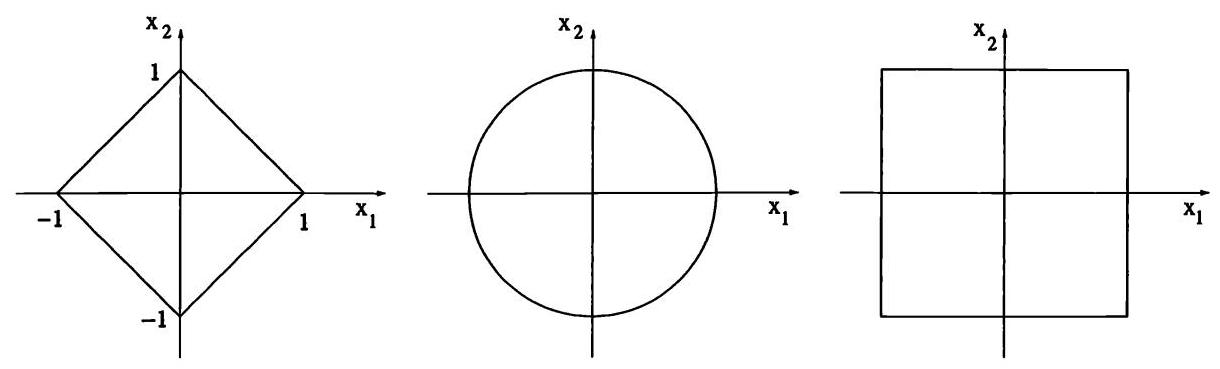
\includegraphics[width=1.0\textwidth]{images/bo_d6ik6nn7aajc739ct1l0_26_134_226_1220_369_0.jpg}
\captionof{figure}{例2.3所述的 \({\mathbb{R}}^{2}\) 中单位球，其范数分别为 \(\|  \cdot  {\| }_{1}\) (左)、 \(\|  \cdot  {\| }_{2}\) (中)和 \(\|  \cdot  {\| }_{\infty }\) (右).}
\end{center}
\hspace*{3em} 


\section{赋范空间与Banach空间的例子.}

\begin{instance}
具有欧氏范数的有限维空间 \({\mathbb{R}}^{n} = \left\{  {x = \left( {{x}_{1},\ldots ,{x}_{n}}\right) ,{x}_{i}}\right. \; \left. { \in  \mathbb{R}}\right\}\)

\begin{equation}\tag{2.2}
\| x{\| }_{2} \doteq  \sqrt{{x}_{1}^{2} + \cdots  + {x}_{n}^{2}}
\end{equation}
是实数域上的Banach空间.特别地，所有实数构成的域 \(\mathbb{R}\) 可视为一维Banach空间.此时，数 \(x \in  \mathbb{R}\) 的范数由其绝对值给出.
\end{instance}

\begin{instance}
    在空间 \({\mathbb{R}}^{n}\) 上可考虑如下替代范数

\[
\| x{\| }_{p} \doteq  {\left( {\left| {x}_{1}\right| }^{p} + \cdots  + {\left| {x}_{n}\right| }^{p}\right) }^{1/p},\;\| x{\| }_{\infty } \doteq  \mathop{\max }\limits_{{1 \leq  i \leq  n}}\left| {x}_{i}\right| .
\]

此处 \(1 \leq  p < \infty\) .这些范数中的每一个亦使 \({\mathbb{R}}^{n}\) 成为有限维Banach空间.
\end{instance}

\begin{instance}
    对任意闭有界区间 \(\left\lbrack  {a,b}\right\rbrack\) ，所有连续函数 \(f : \left\lbrack  {a,b}\right\rbrack   \mapsto  \mathbb{R}\) 构成的空间 \({\mathcal{C}}^{0}\left( \left\lbrack  {a,b}\right\rbrack  \right)\) (赋予范数

\begin{equation}\tag{2.3}
\| f{\| }_{{\mathcal{C}}^{0}} \doteq  \mathop{\max }\limits_{{x \in  \left\lbrack  {a,b}\right\rbrack  }}\left| {f\left( x\right) }\right| ,
\end{equation}
是Banach空间.
\end{instance}

\begin{instance}
    设 \(\Omega\) 为 \({\mathbb{R}}^{n}\) 的开子集.对每个 \(1 \leq  p < \infty\) ，考虑所有勒贝格可测函数 \(f : \Omega  \mapsto  \mathbb{R}\) 构成的空间 \({\mathbf{L}}^{p}\left( \Omega \right)\) ，满足 \({\int }_{\Omega }{\left| f\left( x\right) \right| }^{p}{dx} < \infty\) .此空间在范数

\begin{equation}\tag{2.4}
\| f{\| }_{{\mathbf{L}}^{p}} \doteq  {\left( {\int }_{\Omega }{\left| f\left( x\right) \right| }^{p}dx\right) }^{1/p}.
\end{equation}
下构成Banach空间.此处若两函数 \(f,\widetilde{f}\) 几乎处处相等(即 \(\operatorname{meas}\left( {\{ x \in  \Omega ;f\left( x\right)  \neq  \widetilde{f}\left( x\right) \} }\right)  = 0\) )，则视其为 \({\mathbf{L}}^{p}\left( \Omega \right)\) 中的同一元素.

类似地，所有本质有界、可测函数 \(f : \Omega  \mapsto  \mathbb{R}\) 构成的空间 \({\mathbf{L}}^{\infty }\left( \Omega \right)\) 在范数

\begin{equation}\tag{2.5}
\| f{\| }_{{\mathbf{L}}^{\infty }} \doteq  \underset{x \in  \Omega }{\operatorname{ess}\sup }\left| {f\left( x\right) }\right| .
\end{equation}
\end{instance}

\begin{instance}
    对固定 \(p \geq  1\) ，考虑所有实数序列构成的空间，其 \(p\) 次幂可求和:

\begin{equation}\tag{2.6}
{\ell }^{p} \doteq  \left\{  {\mathbf{x} = \left( {{x}_{1},{x}_{2},\ldots }\right) ;\mathop{\sum }\limits_{{k = 1}}^{\infty }{\left| {x}_{k}\right| }^{p} < \infty }\right\}
\end{equation}

此空间在范数

\begin{equation}\tag{2.7}
\| \mathbf{x}{\| }_{p} \doteq  {\left( \mathop{\sum }\limits_{{k = 1}}^{\infty }{\left| {x}_{k}\right| }^{p}\right) }^{1/p}
\end{equation}

\end{instance}
\begin{instance}
    所有有界实数序列构成的空间 \({\ell }^{\infty }\) (赋予范数

\begin{equation}\tag{2.8}
\| \mathbf{x}{\| }_{\infty } \doteq  \mathop{\sup }\limits_{{k \geq  1}}\left| {x}_{k}\right|
\end{equation}

是Banach空间.在此空间中，可考虑子空间 \({c}_{0}\) ，即所有满足 \(k \rightarrow  \infty\) 时趋于零的序列 \({\left( {x}_{k}\right) }_{k \geq  1}\) 构成的子空间.该子空间在相同范数(2.8)下亦为Banach空间.

\end{instance}

\begin{remark}
    在空间 \({\ell }^{p},1 \leq  p < \infty\) 中，考虑单位向量族(2.9)

\[
{\mathbf{e}}_{1} = \left( {1,0,0,0,\ldots }\right) ,\;{\mathbf{e}}_{2} = \left( {0,1,0,0,\ldots }\right) ,\;{\mathbf{e}}_{3} = \left( {0,0,1,0,\ldots }\right) ,\;\ldots
\]

这些向量线性无关.所有线性组合\footnote{注意，线性组合始终指有限和，而非级数.}

\begin{equation}\tag{2.10}
\operatorname{span}\left\{  {{\mathbf{e}}_{k};k \geq  1}\right\}   = \left\{  {\mathop{\sum }\limits_{{k = 1}}^{N}{\theta }_{k}{\mathbf{e}}_{k};N \geq  1,{\theta }_{k} \in  \mathbb{R}}\right\}
\end{equation}
并不等于整个空间 \({\ell }^{p}\) ，但构成 \({\ell }^{p}\) 的一个稠密子集.事实上，它由形如 \(x = \left( {{x}_{1},{x}_{2},\ldots ,{x}_{N},0,0,0,\ldots }\right)\) 且仅有有限个非零项的序列全体组成.

集合 \(\left\{  {{\mathbf{e}}_{k};k \geq  1}\right\}\) 并非 \({\ell }^{p}\) 的代数基，但提供了一个拓扑基:即每个元素 \(\mathbf{x} = \left( {{x}_{1},{x}_{2},\ldots }\right)  \in  {\ell }^{p}\) 均可表为收敛级数

\[
\mathbf{x} = \mathop{\sum }\limits_{{k = 1}}^{\infty }{x}_{k}{\mathbf{e}}_{k}
\]
\end{remark}
\begin{remark}
    在实数域或复数域上，绝对值 \(\left| \alpha \right|\) 刻画了数 \(\alpha\) 的大小.类似地，在向量空间 \(X\) 上，范数 \(\| f\|\) 可视为刻画元素 \(f \in  X\) 的大小.然而我们注意到，可在同一函数空间上采用不同的范数(从而得到不同的距离)，进而获得截然不同的收敛结果.下一例将对此加以说明.
\end{remark}

例 2.10．设 \(X\) 为区间 \(\left\lbrack  {0,1}\right\rbrack\) 上所有多项式函数构成的空间.在 \(X\) 上可考虑如下两个范数

\begin{equation}\tag{2.11}
\| f{\| }_{{\mathcal{C}}^{0}} \doteq  \mathop{\max }\limits_{{x \in  \left\lbrack  {0,1}\right\rbrack  }}\left| {f\left( x\right) }\right| ,\;\| f{\| }_{{\mathbf{L}}^{1}} \doteq  {\int }_{0}^{1}\left| {f\left( x\right) }\right| {dx}.
\end{equation}

这两个范数给出不同的收敛结果(见图 2.1.2).例如，考虑单项式序列 \({f}_{n}\left( x\right)  = {x}^{n}\) .令 \(n \rightarrow  \infty\) ，则有 \({\begin{Vmatrix}{f}_{n}\end{Vmatrix}}_{{\mathbf{L}}^{1}} \rightarrow  0\) .因此序列 \({\left( {f}_{n}\right) }_{n \geq  1}\) 在 \({\mathbf{L}}^{1}\) 范数下收敛于零(即恒等于零的函数).另一方面，对所有 \(n \geq  1\) 均有 \({\begin{Vmatrix}{f}_{n}\end{Vmatrix}}_{{\mathcal{C}}^{0}} = 1\) .就 \({\mathcal{C}}^{0}\) 范数而言，该序列并非柯西列，且无任何极限.

\begin{center}
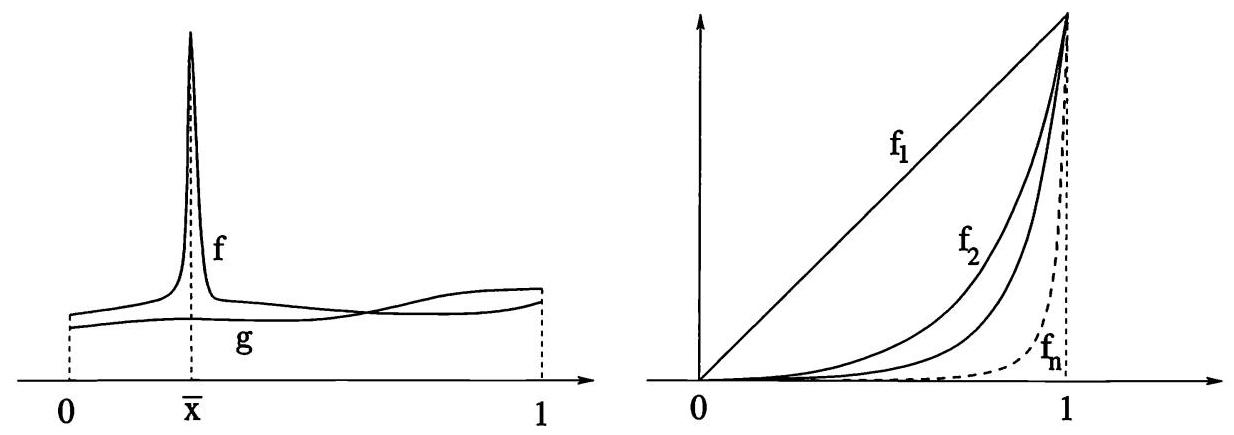
\includegraphics[width=1.0\textwidth]{images/bo_d6ik6nn7aajc739ct1l0_28_122_1102_1234_435_0.jpg}
\end{center}
\hspace*{3em} 

图 2.1.2．左:由阴影区域面积所度量的两函数 \(f,g\) 之间的 \({\mathbf{L}}^{1}\) 距离较小；但由 \(\| f - g{\| }_{{\mathcal{C}}^{0}} = \left| {f\left( \bar{x}\right)  - g\left( \bar{x}\right) }\right|\) 所度量的它们的 \({\mathcal{C}}^{0}\) 距离却很大.右:多项式序列 \({f}_{n}\left( x\right)  = {x}^{n}\) 在空间 \({\mathbf{L}}^{1}\left( \left\lbrack  {0,1}\right\rbrack  \right)\) 中收敛于零，但在空间 \({\mathcal{C}}^{0}\left( \left\lbrack  {0,1}\right\rbrack  \right)\) 中无任何极限.

\section*{2.2．线性算子}

设 \(X,Y\) 是同一标量数域 \(\mathbb{K}\) 上的赋范空间.线性算子是指从子空间 \(\operatorname{Dom}\left( \Lambda \right)  \subseteq  X\) 到 \(Y\) 的映射 \(\Lambda\) ，满足

\[
\Lambda \left( {{c}_{1}{x}_{1} + {c}_{2}{x}_{2}}\right)  = {c}_{1}\Lambda {x}_{1} + {c}_{2}\Lambda {x}_{2}\;\text{ for all }{x}_{1},{x}_{2} \in  \operatorname{Dom}\left( \Lambda \right) ,{c}_{1},{c}_{2} \in  \mathbb{K}.
\]

此处 \(\operatorname{Dom}\left( \Lambda \right)\) 是 \(\Lambda\) 的定义域. \(\Lambda\) 的值域是子空间

\[
\operatorname{Range}\left( \Lambda \right)  \doteq  \{ {\Lambda x};x \in  \operatorname{Dom}\left( \Lambda \right) \}  \subset  Y.
\]

\(\Lambda\) 的零空间(或核)是子空间

\[
\operatorname{Ker}\left( \Lambda \right)  \doteq  \{ x \in  X;{\Lambda x} = 0\}  \subseteq  X.
\]

注意， \(\Lambda\) 是单射当且仅当 \(\operatorname{Ker}\left( \Lambda \right)  = \{ 0\}\) .

接下来，考虑定义在整个空间 \(X\) 上的线性算子 \(\Lambda  : X \mapsto  Y\) ，即满足 \(\operatorname{Dom}\left( \Lambda \right)  = X\) .若 \(\Lambda\) 满足以下条件，则称其为有界的:

\begin{equation}\tag{2.12}
\| \Lambda \|  \doteq  \mathop{\sup }\limits_{{\| x\|  \leq  1}}\| {\Lambda x}\|  < \infty .
\end{equation}
\begin{theorem}[有界算子的连续性]
    线性算子 \(\Lambda  : X \mapsto  Y\) 有界当且仅当它连续.
\end{theorem}
定理 2.11()．

证明:1. 若 \(\Lambda\) 连续，则特别地，它在原点处连续.因此存在 \(\delta  > 0\) ，使得 \(\| x\|  \leq  \delta\) 蕴含 \(\| {\Lambda x}\|  \leq  1\) .由线性性，这表明

\[
\| {\Lambda x}\|  \leq  \frac{1}{\delta }\;\text{ whenever }\;\| x\|  \leq  1.
\]

故 \(\Lambda\) 有界.

2. 反之，设 \(\Lambda\) 有界，即(2.12)成立.由线性性可得

\[
\begin{Vmatrix}{\Lambda {x}_{1} - \Lambda {x}_{2}}\end{Vmatrix} = \begin{Vmatrix}{\Lambda \left( {{x}_{1} - {x}_{2}}\right) }\end{Vmatrix} = \begin{Vmatrix}{{x}_{1} - {x}_{2}}\end{Vmatrix}\begin{Vmatrix}{\Lambda \left( \frac{{x}_{1} - {x}_{2}}{\begin{Vmatrix}{x}_{1} - {x}_{2}\end{Vmatrix}}\right) }\end{Vmatrix} \leq  \begin{Vmatrix}{{x}_{1} - {x}_{2}}\end{Vmatrix}\begin{Vmatrix}\Lambda \end{Vmatrix}.
\]

故 \(\Lambda\) 一致Lipschitz连续，Lipschitz常数为 \(\| \Lambda \|\) .

若 \(X,Y\) 是同一标量域上的赋范空间，我们用 \(\mathcal{B}\left( {X;Y}\right)\) 表示从 \(X\) 到 \(Y\) 的有界线性算子空间.注意此处要求这些算子的定义域为整个空间 \(X\) .

定理2.12(有界线性算子空间):从 \(X\) 到 \(Y\) 的所有有界线性算子构成的空间 \(\mathcal{B}\left( {X;Y}\right)\) 是一个赋范空间，其范数由(2.12)定义；若 \(Y\) 是Banach空间，则 \(\mathcal{B}\left( {X;Y}\right)\) 也是Banach空间.

证明:若 \({\Lambda }_{1},{\Lambda }_{2}\) 是线性算子，且 \({\mathrm{c}}_{1},{\mathrm{c}}_{2} \in  \mathbb{K}\) ，则其线性组合定义为

\[
\left( {{\mathrm{c}}_{1}{\Lambda }_{1} + {c}_{2}{\Lambda }_{2}}\right) \left( x\right)  \doteq  {\mathrm{c}}_{1}{\Lambda }_{1}x + {\mathrm{c}}_{2}{\Lambda }_{2}x.
\]

现验证范数的性质(N1)-(N3)均成立.

1. 若 \(\Lambda  = 0\) 是零算子，则对所有 \(x \in  X\) 有 \({\Lambda x} = 0\) ，且 \(\| \Lambda \|  = 0\) .反之，若 \(\Lambda\) 不是零算子，则存在某个 \(x \neq  0\) 使得 \({\Lambda x} \neq  0\) .故 \(\Lambda \left( \frac{x}{\| x\| }\right)  = \frac{1}{\| x\| }{\Lambda x} \neq  0\) ，且(2.12)中的上确界严格为正.这证明了(N1).

2. 若 \(\alpha  \in  \mathbb{K}\) ，则(N2)由如下恒等式推出

\[
\| {\alpha \Lambda }\|  = \mathop{\sup }\limits_{{\| x\|  \leq  1}}\| {\alpha \Lambda x}\|  = \left| \alpha \right| \mathop{\sup }\limits_{{\| x\|  \leq  1}}\| {\Lambda x}\|  = \left| \alpha \right| \| \Lambda \| .
\]

3. 为验证三角不等式(N3)，对任意满足 \(\| x\|  \leq  1\) 的 \(x \in  X\) ，我们写出

\[
\begin{Vmatrix}{\left( {{\Lambda }_{1} + {\Lambda }_{2}}\right) x}\end{Vmatrix} = \begin{Vmatrix}{{\Lambda }_{1}x + {\Lambda }_{2}x}\end{Vmatrix} \leq  \begin{Vmatrix}{{\Lambda }_{1}x}\end{Vmatrix} + \begin{Vmatrix}{{\Lambda }_{2}x}\end{Vmatrix} \leq  \begin{Vmatrix}{\Lambda }_{1}\end{Vmatrix} + \begin{Vmatrix}{\Lambda }_{2}\end{Vmatrix}.
\]

对所有满足 \(\| x\|  \leq  1\) 的 \(x \in  X\) 取上确界，即得(N3).

4. 接着，假设 \(Y\) 是Banach空间.需证 \(\mathcal{B}\left( {X;Y}\right)\) 完备.设 \({\left( {\Lambda }_{n}\right) }_{n \geq  1}\) 是一列有界线性算子的Cauchy列.对每个 \(x \in  X\) ，这蕴含

\[
\mathop{\limsup }\limits_{{m,n \rightarrow  \infty }}\begin{Vmatrix}{{\Lambda }_{m}x - {\Lambda }_{n}x}\end{Vmatrix} \leq  \mathop{\limsup }\limits_{{m,n \rightarrow  \infty }}\begin{Vmatrix}{{\Lambda }_{m} - {\Lambda }_{n}}\end{Vmatrix}\| x\|  = 0.
\]

因此点列 \({\left( {\Lambda }_{n}x\right) }_{n \geq  1}\) 在 \(Y\) 中为Cauchy列.由于 \(Y\) 完备，该列有唯一极限，记为 \({\Lambda x}\) .

因每个 \({\Lambda }_{n}\) 均为线性算子，显然 \(\Lambda\) 亦为线性算子.我们断言 \(\Lambda\) 亦有界(从而连续).由假设，可选取足够大的 \(N\) 使得

\[
\begin{Vmatrix}{{\Lambda }_{k} - {\Lambda }_{N}}\end{Vmatrix} \leq  1\;\text{ for all }k \geq  N.
\]

因此，对任意满足 \(\| x\|  \leq  1\) 的 \(x \in  X\) ，均有

\[
\| {\Lambda x}\|  = \mathop{\lim }\limits_{{k \rightarrow  \infty }}\begin{Vmatrix}{{\Lambda }_{k}x}\end{Vmatrix} \leq  \begin{Vmatrix}{{\Lambda }_{N}x}\end{Vmatrix} + \mathop{\limsup }\limits_{{k \rightarrow  \infty }}\begin{Vmatrix}{{\Lambda }_{k} - {\Lambda }_{N}}\end{Vmatrix}\| x\|  \leq  \begin{Vmatrix}{\Lambda }_{N}\end{Vmatrix} + 1.
\]

由于 \(x\) 是单位球中的任意一点，这证明极限算子 \(\Lambda\) 有界，从而 \(\Lambda  \in  \mathcal{B}\left( {X;Y}\right)\) .

\section*{2.2.1. 线性算子示例.}

例2.13(矩阵作为线性算子).每个 \(n \times  m\) 矩阵 \(A = \left( {a}_{ij}\right)\) 确定一个由下式定义的有界线性算子 \(\Lambda  : {\mathbb{R}}^{m} \mapsto  {\mathbb{R}}^{n}\) :

\[
\Lambda \left( {{x}_{1},\ldots ,{x}_{m}}\right)  = \left( {{y}_{1},\ldots ,{y}_{n}}\right) ,\;\text{ with }\;{y}_{i} \doteq  \mathop{\sum }\limits_{{j = 1}}^{m}{a}_{ij}{x}_{j}.
\]

例2.14(序列空间上的对角算子).设 \(1 \leq  p \leq  \infty\) ，并考虑所有实数序列 \(\mathbf{x} = \left( {{x}_{1},{x}_{2},\ldots }\right)\) 构成的空间 \(X = {\ell }^{p}\) ，其范数按(2.7)或(2.8)式定义.设 \(\left( {{\lambda }_{1},{\lambda }_{2},\ldots }\right)\) 为任意实数序列，并将算子 \(\Lambda  : X \mapsto  X\) 定义为:

\begin{equation}\tag{2.13}
\Lambda \left( {{x}_{1},{x}_{2},{x}_{3},\ldots }\right)  \doteq  \left( {{\lambda }_{1}{x}_{1},{\lambda }_{2}{x}_{2},{\lambda }_{3}{x}_{3},\ldots }\right) .
\end{equation}

参照(2.9)式中单位向量基 \(\left\{  {{\mathbf{e}}_{1},{\mathbf{e}}_{2},\ldots }\right\}\) ，可将 \(\Lambda\) 视作一个无穷矩阵:

\[
\left( \begin{matrix} {\lambda }_{1} & 0 & & & \\  0 & {\lambda }_{2} & & & \\   & & {\lambda }_{3} & & \\   & & & &  \end{matrix}\right)
\]

其对角线元素为 \({\lambda }_{1},{\lambda }_{2},\ldots\) ，其余位置均为0.此时我们分两种情形.

(i) 若序列 \({\left( {\lambda }_{k}\right) }_{k \geq  1}\) 有界，则算子 \(\Lambda\) 有界，其范数为

\begin{equation}\tag{2.14}
\| \Lambda \|  = \mathop{\sup }\limits_{k}\left| {\lambda }_{k}\right|
\end{equation}

(ii) 若序列 \({\left( {\lambda }_{k}\right) }_{k \geq  1}\) 无界，则算子 \(\Lambda\) 无界，其定义域

\[
\operatorname{Dom}\left( \Lambda \right)  = \left\{  {x \in  {\ell }^{p};{\Lambda x} \in  {\ell }^{p}}\right\}
\]

是一个向量子空间，且严格包含于 \({\ell }^{p}\) 中.

例2.15(微分算子).考虑开区间 \(I = \rbrack 0,\pi \lbrack\) ，令 \(X = \mathcal{B}C\left( I\right)\) 为 \(I\) 上所有有界连续实值函数构成的空间，其范数为

\[
\| f\|  = \mathop{\sup }\limits_{{0 < x < \pi }}\left| {f\left( x\right) }\right| .
\]

\({\Lambda f} = {f}^{\prime }\) 微分算子显然是 \(X\) 上的线性算子.为说明该算子无界，考虑函数列 \({f}_{k}\left( x\right)  = \sin {kx}\) .此时 \({f}_{k}^{\prime }\left( x\right)  = k\cos {kx}\) ，故

\[
\begin{Vmatrix}{f}_{k}\end{Vmatrix} = 1,\;\begin{Vmatrix}{\Lambda {f}_{k}}\end{Vmatrix} = k\;\text{ for all }k \geq  1.
\]

该微分算子的定义域 \(\operatorname{Dom}\left( \Lambda \right)\) 是所有处处可微、且导数有界连续的有界连续函数 \(f : I \mapsto  \mathbb{R}\) 构成的空间.这是 \(\mathcal{B}C\left( I\right)\) 的一个真子空间.

例2.16( \({\mathbf{L}}^{p}\left( \mathbb{R}\right)\) 上的移位算子).令 \(1 \leq  p \leq  \infty\) .任取 \(a \in  \mathbb{R}\) .对任意函数 \(f \in  {\mathbf{L}}^{p}\left( \mathbb{R}\right)\) ，定义 \(\left( {{\Lambda }_{a}f}\right) \left( x\right)  \doteq  f\left( {x - a}\right)\) .显然 \(\| {\Lambda f}{\| }_{{\mathbf{L}}^{p}} = \| f{\| }_{{\mathbf{L}}^{p}}\) .因此 \({\Lambda }_{a} : {\mathbf{L}}^{p} \mapsto  {\mathbf{L}}^{p}\) 是有界线性算子，其范数为 \(\begin{Vmatrix}{\Lambda }_{a}\end{Vmatrix} = 1\) .注意，算子 \({\Lambda }_{a}\) 是一一映射且满射.

例2.17( \({\ell }^{p}\) 上的移位算子).令 \(1 \leq  p \leq  \infty\) .定义算子 \({\Lambda }_{ + } : {\ell }^{p} \mapsto  {\ell }^{p}\) 与 \({\Lambda }_{ - } : {\ell }^{p} \mapsto  {\ell }^{p}\) 如下:

\[
{\Lambda }_{ + }\left( {{x}_{1},{x}_{2},{x}_{3},\ldots }\right)  \doteq  \left( {0,{x}_{1},{x}_{2},\ldots }\right)
\]

\[
{\Lambda }_{ - }\left( {{x}_{1},{x}_{2},{x}_{3},\ldots }\right)  \doteq  \left( {{x}_{2},{x}_{3},{x}_{4},\ldots }\right)
\]

注意到它们均为线性连续算子，且满足 \(\begin{Vmatrix}{\Lambda }_{ + }\end{Vmatrix} = \begin{Vmatrix}{\Lambda }_{ - }\end{Vmatrix} = 1\) .此外， \({\Lambda }_{ + }\) 是一一映射但非满射，而 \({\Lambda }_{ - }\) 是满射但非一一映射.

例2.18(乘法算子).设 \(\Omega  \subset  {\mathbb{R}}^{n}\) ，且 \(g : \Omega  \mapsto  \mathbb{R}\) 为一有界可测函数.对任意 \(1 \leq  p \leq  \infty\) ，在空间 \({\mathbf{L}}^{p}\left( \Omega \right)\) 上考虑乘法算子: \(\left( {{M}_{g}f}\right) \left( x\right)  \doteq  g\left( x\right) f\left( x\right)\) .该算子连续，其范数为

\begin{equation}\tag{2.15}
\begin{Vmatrix}{M}_{g}\end{Vmatrix} \doteq  \mathop{\sup }\limits_{{\| f{\| }_{{\mathbf{L}}^{p}} \leq  1}}\| {gf}{\| }_{{\mathbf{L}}^{p}} = \| g{\| }_{{\mathbf{L}}^{\infty }}.
\end{equation}

例2.19(积分算子).设 \(a < b\) ，并考虑定义在闭区间 \(\left\lbrack  {a,b}\right\rbrack\) 上的实值连续函数空间 \(X = {\mathcal{C}}^{0}\left( \left\lbrack  {a,b}\right\rbrack  \right)\) .考虑积分算子

\[
\left( {\Lambda f}\right) \left( x\right)  \doteq  {\int }_{a}^{x}f\left( y\right) {dy}.
\]

则 \(\Lambda  : X \mapsto  X\) 是有界线性算子.事实上，

\[
\left| {\left( {\Lambda f}\right) \left( x\right) }\right| \; = \;\left| {{\int }_{a}^{x}f\left( y\right) \;{dy}}\right| \; \leq  \;{\int }_{a}^{x}\left| {f\left( y\right) }\right| \;{dy}\; \leq  \;\left( {b - a}\right)  \cdot  \mathop{\max }\limits_{{x \in  \left\lbrack  {a,b}\right\rbrack  }}\left| {f\left( x\right) }\right| .
\]

因此 \(\| {\Lambda f}\|  \leq  \left( {b - a}\right) \| f\|\) 且 \(\| \Lambda \|  \leq  \left( {b - a}\right)\) .

\section*{2.3 有限维空间}

我们称同一向量空间 \(X\) 上的两个范数 \(\|  \cdot  {\| }_{\diamond }\) 与 \(\|  \cdot  {\| }_{\diamond }\) 等价，若存在常数 \(C \geq  1\) ，使得

\begin{equation}\tag{2.16}
\frac{1}{C}\| x{\| }_{\diamond } \leq  \| x{\| }_{\spadesuit } \leq  C\| x{\| }_{\diamond }\;\text{ for all }x \in  X.
\end{equation}

等价范数在 \(X\) 上给出相同的柯西列和相同的拓扑.一般而言，无限维空间 \(X\) 可具有许多互不等价的范数.如例2.10所示，在单实变量多项式全体构成的空间上， \({\mathbf{L}}^{1}\) 范数与(2.11)式中定义的 \({\mathcal{C}}^{0}\) 范数并不等价.

接下来的结果表明:对任意有限维向量空间 \(X\) ，其所有范数均等价.事实上，每个维数为 \(N\) 的有限维赋范空间均与欧几里得空间 \({\mathbb{K}}^{N}\) 等价.我们回顾:向量 \(\alpha  = \left( {{\alpha }_{1},\ldots ,{\alpha }_{N}}\right)  \in  {\mathbb{K}}^{N}\) 的欧几里得范数为 \(\| \alpha \|  \doteq  \sqrt{\mathop{\sum }\limits_{k}{\left| {\alpha }_{k}\right| }^{2}}\) .

定理2.20(有限维赋范空间同胚于 \({\mathbb{K}}^{N}\) ).设 \(X\) 为定义在实数或复数域 \(\mathbb{K}\) 上的有限维赋范空间， \(\mathcal{B} = \left\{  {{u}_{1},{u}_{2},\ldots ,{u}_{N}}\right\}\) 为其一组基.则

(i) \(X\) 完备，因而为Banach空间.

(ii) 对每个 \(\alpha  = \left( {{\alpha }_{1},{\alpha }_{2},\ldots ,{\alpha }_{N}}\right)  \in  {\mathbb{K}}^{N}\) ，定义

\begin{equation}\tag{2.17}
{\Lambda \alpha } \doteq  {\alpha }_{1}{u}_{1} + {\alpha }_{2}{u}_{2} + \cdots  + {\alpha }_{N}{u}_{N}.
\end{equation}

则线性算子 \(\Lambda  : {\mathbb{K}}^{N} \mapsto  X\) 是双射且有界的.此外，其逆算子 \({\Lambda }^{-1} : X \mapsto  {\mathbb{K}}^{N}\) 亦有界.

证明.1. \(\left\{  {{u}_{1},\ldots ,{u}_{N}}\right\}\) 为基这一事实意味着 \(\Lambda\) 是单射且满射，故逆算子 \({\Lambda }^{-1} : X \mapsto  {\mathbb{K}}^{N}\) 良定义.

2. 将

\[
\| {\Lambda \alpha }\|  \leq  \mathop{\sum }\limits_{{k = 1}}^{N}\begin{Vmatrix}{{\alpha }_{k}{u}_{k}}\end{Vmatrix} \leq  \| \alpha \| \mathop{\sum }\limits_{{k = 1}}^{N}\begin{Vmatrix}{u}_{k}\end{Vmatrix},
\]

展开可见， \(\Lambda  : {\mathbb{K}}^{N} \mapsto  X\) 为有界线性算子，因而连续.

3. 我们断言 \({\Lambda }^{-1}\) 也有界.否则，存在 \(X\) 中的一个序列 \({\left( {x}_{n}\right) }_{n \geq  1}\) ，使得对每个 \(n\) 均有 \(\begin{Vmatrix}{x}_{n}\end{Vmatrix} \leq  1\) ，且

\[
\begin{Vmatrix}{{\Lambda }^{-1}{x}_{n}}\end{Vmatrix} \rightarrow  \infty \;\text{ as }n \rightarrow  \infty .
\]

考虑归一化向量

\[
{\beta }_{n} \doteq  \frac{{\Lambda }^{-1}{x}_{n}}{\begin{Vmatrix}{\Lambda }^{-1}{x}_{n}\end{Vmatrix}} \in  {\mathbb{K}}^{N}.
\]

于是 \(\begin{Vmatrix}{\beta }_{n}\end{Vmatrix} = 1\) 且 \(\Lambda {\beta }_{n} \rightarrow  0\) 当 \(n \rightarrow  \infty\) 时成立.由于 \({\left( {\beta }_{n}\right) }_{n \geq  1}\) 是欧几里得空间 \({\mathbb{K}}^{N}\) 中的有界序列，故存在收敛子列，记为 \({\beta }_{{n}_{k}} \rightarrow  \beta  \in  {\mathbb{K}}^{N}\) .显然

\[
\| \beta \| \; = \;\mathop{\lim }\limits_{{k \rightarrow  \infty }}\begin{Vmatrix}{\beta }_{{n}_{k}}\end{Vmatrix}\; = \;1,\;{\Lambda \beta }\; = \;\mathop{\lim }\limits_{{k \rightarrow  \infty }}\Lambda {\beta }_{{n}_{k}}\; = \;\mathop{\lim }\limits_{{k \rightarrow  \infty }}\frac{{x}_{{k}_{n}}}{\begin{Vmatrix}{\Lambda }^{-1}{x}_{{k}_{n}}\end{Vmatrix}}\; = \;0\;,
\]

因为 \(\Lambda\) 连续.这与 \(\Lambda\) 是单射相矛盾.因此我们得出结论: \({\Lambda }^{-1}\) 有界，从而连续.这就证明了 (ii).

4. 为证范数为 \(\|  \cdot  \|\) 的 \(X\) 完备，设 \({\left( {x}_{n}\right) }_{n \geq  1}\) 是 \(X\) 中的柯西序列.则 \({\Lambda }^{-1}{x}_{n}\) 在 \({\mathbb{K}}^{N}\) 中构成柯西序列；由于 \({\mathbb{K}}^{N}\) 完备，该序列收敛于某点 \(\beta  \in  {\mathbb{K}}^{N}\) .又因 \(\Lambda\) 连续，故序列 \({x}_{n}\) 收敛于 \({\Lambda \beta }\) .

推论 2.21. 在有限维空间中，所有范数均等价.

证明. 设 \(\|  \cdot  {\| }_{\diamond }\) 和 \(\|  \cdot  {\| }_{\diamond }\) 是有限维向量空间 \(X\) 上的任意两个范数.令 \(\mathcal{B} = \left\{  {{u}_{1},\ldots ,{u}_{N}}\right\}\) 是 \(X\) 的一组基，并如 (2.17) 式定义线性映射 \(\Lambda  : {\mathbb{K}}^{N} \mapsto  X\) .由前述定理， \(\Lambda\) 与 \({\Lambda }^{-1}\) 均为有界线性算子(在 \(X\) 的这两种范数下).因此存在常数 \({C}^{\prime },{C}^{\prime \prime }\) ，使得

\[
\frac{1}{{C}^{\prime }}\begin{Vmatrix}{{\Lambda }^{-1}x}\end{Vmatrix} \leq  \| x{\| }_{\diamond } \leq  {C}^{\prime }\begin{Vmatrix}{{\Lambda }^{-1}x}\end{Vmatrix}
\]

\[
\frac{1}{{C}^{\prime \prime }}\begin{Vmatrix}{{\Lambda }^{-1}x}\end{Vmatrix} \leq  \| x{\| }_{\spadesuit } \leq  {C}^{\prime \prime }\begin{Vmatrix}{{\Lambda }^{-1}x}\end{Vmatrix},
\]

对所有 \(x \in  X\) 成立.这即推出 (2.16) 式.

波尔查诺-Weierstrass经典定理指出: \({\mathbb{R}}^{N}\) 中每个有界序列都存在收敛子列.下一个定理表明，这一紧性性质对所有有限维赋范空间成立，而对所有无限维赋范空间均不成立.

定理 2.22(局部紧的赋范空间必为有限维). 设 \(X\) 是一个赋范空间.以下命题等价:

(i) \(X\) 是有限维的.

(ii) 闭单位球 \({B}_{1} \doteq  \overline{B\left( {0,1}\right) } = \{ x \in  X;\| x\|  \leq  1\}\) 是紧的.

\begin{center}
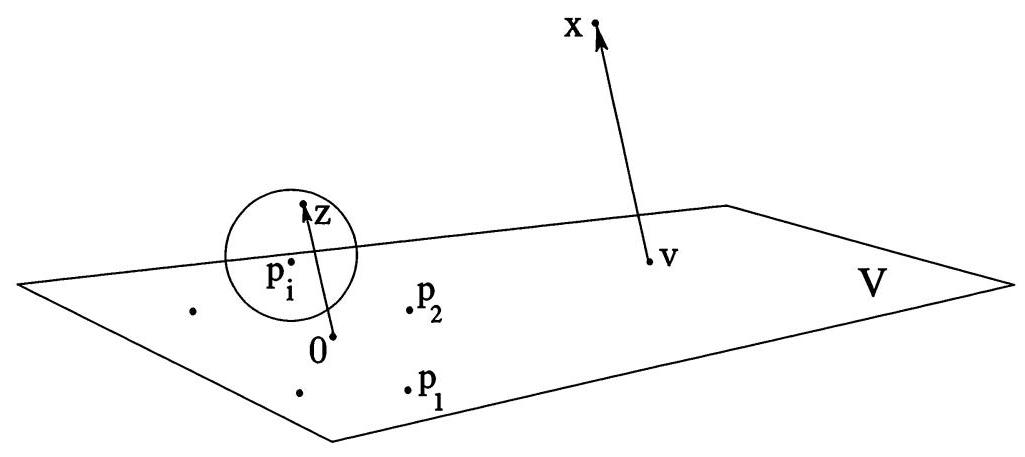
\includegraphics[width=0.9\textwidth]{images/bo_d6ik6nn7aajc739ct1l0_34_221_1328_1025_457_0.jpg}
\end{center}
\hspace*{3em} 

图 2.3.1. 用于证明定理 2.22 的构造.

证明:(i) \(\Rightarrow\) .(ii) 设 \(X\) 的维数为 \(N\) .则由定理 2.20，存在一个具有有界逆的线性同胚映射 \(\Lambda  : {\mathbb{K}}^{N} \mapsto  X\) .由于单位球 \({B}_{1} \subset  X\) 是闭且有界的，故 \(K \doteq \; {\Lambda }^{-1}\left( {B}_{1}\right)  \subset  {\mathbb{K}}^{N}\) 同样闭且有界.由波尔查诺-Weierstrass定理，闭有集 \(K\) 是紧的.而 \({B}_{1} = \Lambda \left( K\right)\) 作为紧集的连续像，亦为紧集.

(ii) \(\Rightarrow\) (i).假设闭单位球 \({B}_{1} \subset  X\) 是紧的，则其是列紧的，可用有限个以点 \({p}_{i},i = 1,\ldots ,n\) 为中心、半径为 \(1/2\) 的开球 \(B\left( {{p}_{i},1/2}\right)\) 覆盖.考虑有限维子空间 \(V = \operatorname{span}\left\{  {{p}_{1},\ldots ,{p}_{n}}\right\}\) (见图 2.3.1).注意 \(V\) 在 \(X\) 中是闭的，因为根据定理 2.20，每个有限维赋范空间都是完备的.

我们断言 \(V = X\) ，从而 \(X\) 本身是有限维的.否则，可找到一点 \(x \in  X \setminus  V\) .令 \(\rho  \doteq  d\left( {x,V}\right)  \doteq  \mathop{\inf }\limits_{{y \in  V}}\| y - x\|\) .注意到 \(\rho  > 0\) ，因为 \(V\) 是闭的.因此存在一点 \(v \in  V\) ，使得

\begin{equation}\tag{2.18}
\rho  \leq  \| x - v\|  \leq  \frac{3}{2}\rho .
\end{equation}

考虑单位向量

\[
z \doteq  \frac{x - v}{\| x - v\| } \in  {B}_{1}.
\]

由构造可知，存在一点 \({p}_{i} \in  {B}_{1}\) ，使得 \(\begin{Vmatrix}{z - {p}_{i}}\end{Vmatrix} < \frac{1}{2}\) .于是我们有

\[
x = v + \| x - v\| z = v + \| x - v\| {p}_{i} + \| x - v\| \left( {z - {p}_{i}}\right) .
\]

由于 \(v + \| x - v\| {p}_{i} \in  V\) ，必有

\[
\| x - v\| \begin{Vmatrix}{z - {p}_{i}}\end{Vmatrix} \geq  d\left( {x,V}\right)  \geq  \rho .
\]

故 \(\| x - v\|  \geq  {2\rho }\) ，与 (2.18) 矛盾.这表明 \(X = V\) ，证毕.

\section*{2.4. 半范数与Fr空间}

为引出半范数的概念，我们注意到:对某些函数空间而言，并不存在定义范数的自然方式.

例 2.23.考虑开区间 ] \(0,1\lbrack\) 上所有连续(可能无界)函数构成的空间 \(X \doteq  \mathcal{C}\left( {\rbrack 0,1\lbrack }\right)\) .若定义

\[
p\left( f\right)  \doteq  \mathop{\sup }\limits_{{0 < x < 1}}\left| {f\left( x\right) }\right| ,
\]

则该式不能在整个空间 \(X\) 上给出一个范数.事实上，只要 \(f\) 无界，右端即取值为 \(+ \infty\) .

另一方面，对任意闭子区间 \(\left\lbrack  {a,b}\right\rbrack   \subset  \rbrack 0,1\lbrack\) ，“半范数”

\begin{equation}\tag{2.19}
{p}^{a,b}\left( f\right)  \doteq  \mathop{\max }\limits_{{x \in  \left\lbrack  {a,b}\right\rbrack  }}\left| {f\left( x\right) }\right|
\end{equation}

恒为一良定义的实数.注意，式 (2.19) 中的泛函不满足范数的所有要求，因为存在函数 \(f \in  \mathcal{C}\left( {\rbrack 0,1\lbrack }\right)\) 在 \(\left\lbrack  {a,b}\right\rbrack\) 上恒为零但并非恒等于零；此时 \({p}^{a,b}\left( f\right)  = 0\) 而 \(f \neq  0\) .

设 \(X\) 是域 \(\mathbb{K}\) 上的一个向量空间.实值映射 \(x \mapsto  p\left( x\right)\) 称为 \(X\) 上的一个半范数，若其满足如下性质:

(SN1) 对每个 \(x \in  X\) ，有 \(p\left( x\right)  \geq  0\) .

(SN2) 对每个 \(x \in  X\) 和 \(\lambda  \in  \mathbb{K}\) ，有 \(p\left( {\lambda x}\right)  = \left| \lambda \right| p\left( x\right)\) .

(SN3) 对每个 \(x,y \in  X,p\left( {x + y}\right)  \leq  p\left( x\right)  + p\left( y\right)\) .

注意:(SN2)-(SN3) 与范数定义中的完全相同，唯一区别在于 (SN1) 中不要求严格正性条件.换言之，我们允许 \(p\left( x\right)  = 0\) ，即使 \(x \neq  0\) .

若 \(p\left( \cdot \right)\) 是一个半范数，则通过设定 \(d\left( {x,y}\right)  \doteq  p\left( {x - y}\right)\) ，我们并不能保证在空间 \(X\) 上得到一个距离.事实上，即使 \(x \neq  y\) ，也可能有 \(d\left( {x,y}\right)  = \; p\left( {x - y}\right)  = 0\) .然而，存在一些有趣的情形:可通过不止一个、而是可数个半范数来构造距离.

我们称 \(X\) 上的一列半范数 \({\left( {p}_{k}\right) }_{k \geq  1}\) 是分离的，如果对每个满足 \(x \neq  0\) 的 \(x \in  X\) ，均存在至少一个指标 \(k\) ，使得 \({p}_{k}\left( x\right)  > 0\) .

引理 2.24(由半范数生成的距离).设 \({\left( {p}_{k}\right) }_{k \geq  1}\) 是向量空间 \(X\) 上的一列分离半范数.则

\begin{equation}\tag{2.20}
d\left( {x,y}\right)  \doteq  \mathop{\sum }\limits_{{k = 1}}^{\infty }{2}^{-k}\frac{{p}_{k}\left( {x - y}\right) }{1 + {p}_{k}\left( {x - y}\right) }
\end{equation}

在 \(X\) 上定义了一个距离.

证明.恒等式

\[
d\left( {x,x}\right)  = 0,\;d\left( {x,y}\right)  = d\left( {y,x}\right)
\]

是 (SN2) 的直接推论.序列 \(\left( {p}_{k}\right)\) 的分离性保证了只要 \(x \neq  y\) ，就有 \(d\left( {x,y}\right)  > 0\) .

为证三角不等式，注意到若 \(a,b,c \geq  0\) 且 \(c \leq \; a + b\) ，则

\[
\frac{c}{1 + c} \leq  \frac{a + b}{1 + a + b} \leq  \frac{a}{1 + a} + \frac{b}{1 + b}
\]

因为函数 \(s \mapsto  \frac{s}{1 + s}\) 是递增且向下凹的.由 (SN3)，可将上述不等式用于 \(a = {p}_{k}\left( {x - y}\right) ,b = {p}_{k}\left( {y - z}\right) ,c = {p}_{k}\left( {x - z}\right)\) ，得

\[
d\left( {x,z}\right)  = \mathop{\sum }\limits_{{k = 1}}^{\infty }{2}^{-k}\frac{{p}_{k}\left( {x - z}\right) }{1 + {p}_{k}\left( {x - z}\right) }
\]

\[
\leq  \mathop{\sum }\limits_{{k = 1}}^{\infty }{2}^{-k}\left( {\frac{{p}_{k}\left( {x - y}\right) }{1 + {p}_{k}\left( {x - y}\right) } + \frac{{p}_{k}\left( {y - z}\right) }{1 + {p}_{k}\left( {y - z}\right) }}\right)
\]

\[
= d\left( {x,y}\right)  + d\left( {y,z}\right) .
\]

这证明了 \(d\left( {\cdot , \cdot  }\right)\) 确实是一个距离.

由定义可知，距离 (2.20) 在平移下不变，即

\[
d\left( {x,y}\right)  = d\left( {x + z,y + z}\right) \;\text{ for all }x,y,z \in  X.
\]

若向量空间 \(X\) 关于距离 (2.20) 构成完备度量空间，则称 \(X\) 为 Fréchet 空间.

例 2.25.设 \(\Omega  \subseteq  {\mathbb{R}}^{n}\) 为任意开集，其边界为 \(\partial \Omega\) .则所有(可能无界)连续函数 \(f : \Omega  \mapsto  \mathbb{R}\) 构成的空间 \(\mathcal{C}\left( \Omega \right)\) 并无自然范数.但可如下赋予其 Fréchet 空间结构:对每个 \(k \geq  1\) ，考虑紧子集(图 2.4.1)

\begin{equation}\tag{2.21}
{A}_{k} \doteq  \left\{  {x \in  \Omega ;\left| x\right|  \leq  k,d\left( {x,\partial \Omega }\right)  \leq  {k}^{-1}}\right\}  .
\end{equation}

定义半范数

\begin{equation}\tag{2.22}
{p}_{k}\left( f\right)  \doteq  \mathop{\max }\limits_{{x \in  {A}_{k}}}\left| {f\left( x\right) }\right|
\end{equation}

并令 \(d\left( {\cdot , \cdot  }\right)\) 为如(2.20)式所定义的相应距离.

\begin{center}
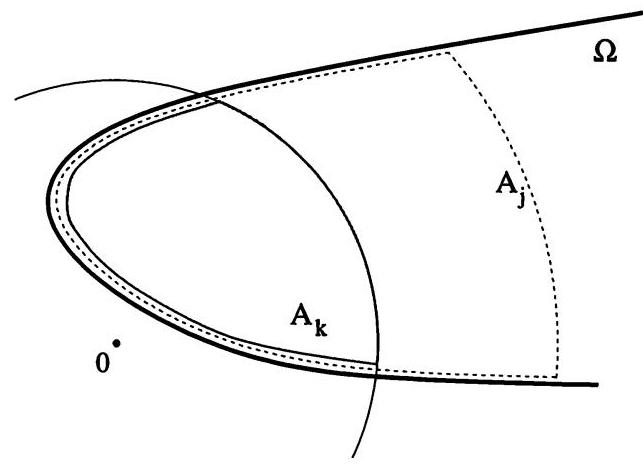
\includegraphics[width=0.6\textwidth]{images/bo_d6ik6nn7aajc739ct1l0_37_413_1667_643_469_0.jpg}
\end{center}
\hspace*{3em} 

图2.4.1:紧子集 \({A}_{k} \subset  \Omega\) .

我们证明:配备上述距离的 \(\mathcal{C}\left( \Omega \right)\) 是一个完备度量空间，因而是一个Fréchet空间.设 \({\left( {f}_{j}\right) }_{j \geq  1}\) 是一个Cauchy列.对每个 \(k\) ，这蕴含

\begin{equation}\tag{2.23}
\mathop{\limsup }\limits_{{i,j \rightarrow  \infty }}{p}_{k}\left( {{f}_{i} - {f}_{j}}\right)  = \mathop{\limsup }\limits_{{i,j \rightarrow  \infty }}\mathop{\sup }\limits_{{x \in  {A}_{k}}}\left| {{f}_{i}\left( x\right)  - {f}_{j}\left( x\right) }\right|  = 0.
\end{equation}

由于每一点 \(x \in  \Omega\) 都包含于某个集合 \({A}_{k}\) 中，由(2.23)式可知序列 \({f}_{j}\left( x\right)\) 是Cauchy列，从而收敛于某个极限 \(f\left( x\right)\) .更一般地，每个紧子集 \(K \subset  \Omega\) 都包含于某个集合 \({A}_{k}\) 中.再次由(2.23)式可知， \({f}_{j} \rightarrow  f\) 的收敛在 \(\Omega\) 的每个紧子集上是一致的，故极限 \(f\) 连续.

接下来只需证明 \(d\left( {{f}_{j},f}\right)  \rightarrow  0\) 当 \(j \rightarrow  \infty\) .对任意固定的 \(m \geq  1\) ，利用 \({f}_{j} \rightarrow  f\) 在紧集 \({A}_{m}\) 上一致收敛这一事实，可得

\[
\mathop{\limsup }\limits_{{j \rightarrow  \infty }}d\left( {{f}_{j},f}\right)
\]

\[
\leq  \mathop{\limsup }\limits_{{j \rightarrow  \infty }}\mathop{\sum }\limits_{{k = 1}}^{m}{2}^{-k}\frac{{p}_{k}\left( {{f}_{j} - f}\right) }{1 + {p}_{k}\left( {{f}_{j} - f}\right) } + \mathop{\limsup }\limits_{{j \rightarrow  \infty }}\mathop{\sum }\limits_{{k = m + 1}}^{\infty }{2}^{-k}\frac{{p}_{k}\left( {{f}_{j} - f}\right) }{1 + {p}_{k}\left( {{f}_{j} - f}\right) }
\]

\[
\leq  0 + {2}^{-m}\text{ . }
\]

由于 \(m\) 是任意的，收敛性得证.

例2.26(空间 \({\mathbf{L}}_{\text{ loc }}^{p}\) ).与前一例类似，设 \(\Omega  \subseteq  {\mathbb{R}}^{n}\) 为开集.若开集 \({\Omega }^{\prime }\) 的闭包 \({\overline{\Omega }}^{\prime }\) 是 \(\Omega\) 的紧子集，则称 \({\Omega }^{\prime }\) 紧含于 \(\Omega\) ，记作 \({\Omega }^{\prime } \subset   \subset  \Omega\) .

对 \(p \in  \left\lbrack  {1,\infty \left\lbrack  \right. }\right.\) ，定义 \({\mathbf{L}}_{\text{ loc }}^{p}\left( \Omega \right)\) 为所有可测函数 \(f\) 构成的空间，使得对每个紧含于 \(\Omega\) 的开集 \({\Omega }^{\prime }\) 均有 \({\int }_{{\Omega }^{\prime }}{\left| f\right| }^{p}{dx} < \infty\) .该空间未赋予自然范数.然而，对每个 \(k \geq  1\) ，可考虑半范数

\begin{equation}\tag{2.24}
{p}_{k}\left( f\right)  \doteq  {\left( {\int }_{{A}_{k}}{\left| f\right| }^{p}dx\right) }^{1/p} = \| f{\| }_{{\mathbf{L}}^{p}\left( {A}_{k}\right) },
\end{equation}

其中 \({A}_{k}\) 是(2.21)式中定义的集合.相应的距离(2.20)使 \({\mathbf{L}}_{\text{ loc }}^{p}\left( \Omega \right)\) 成为一个Fréchet空间.

\section*{2.5 扩张定理}

设 \(X\) 是域 \(\mathbb{K}\) 上的向量空间.线性映射 \(F : X \mapsto  \mathbb{K}\) 称为 \(X\) 上的线性泛函.本节的最终目标是证明存在大量连续线性泛函.为此，我们首先证明一个扩张定理:给定定义在子空间 \(\mathbb{K}\) 上的线性泛函

\(f : V \mapsto  \mathbb{K}\) 定义在子空间 \(V \subset  X\) 上，可将其延拓为定义在整个空间上的泛函 \(F : X \mapsto  \mathbb{K}\) ，同时保持某些附加性质.

以下考虑实数域上的向量空间 \(X\) ，并设 \(p : X \mapsto  \mathbb{R}\) 是满足如下条件的函数:

\[
\text{ ) }p\left( {x + y}\right)  \leq  p\left( x\right)  + p\left( y\right) ,\;p\left( {tx}\right)  = {tp}\left( x\right) \text{ for all }x,y \in  X,t \geq  0\text{ . }
\]

注2.27:若 \(X\) 是赋范空间，则对任意 \(\kappa  > 0\) ，函数 \(p\left( x\right)  = \kappa \| x\|\) 均满足上述性质.更一般地，任一半范数也满足(2.25)式.

注意到(2.25)式表明函数 \(p\) 是凸的.事实上

\[
p\left( {{\theta x} + \left( {1 - \theta }\right) y}\right)  \leq  p\left( {\theta x}\right)  + p\left( {\left( {1 - \theta }\right) y}\right)  = {\theta p}\left( x\right)  + \left( {1 - \theta }\right) p\left( y\right)
\]

对所有 \(x,y \in  X,\theta  \in  \left\lbrack  {0,1}\right\rbrack\) 成立.然而，与半范数相比，此处我们还允许 \(p\left( x\right)  < 0\) .此外，我们并不要求 \(p\) 关于原点对称.换言之，完全可能有 \(p\left( x\right)  \neq  p\left( {-x}\right)\) .

例2.28.设 \(X\) 为赋范空间， \(\Omega  \subset  X\) 为包含原点的有界开凸集.则泛函

\begin{equation}\tag{2.26}
p\left( x\right)  \doteq  \inf \{ \lambda  \geq  0;x \in  {\lambda \Omega }\}
\end{equation}

满足假设(2.25).

定理2.29(哈恩-Banach延拓定理).设 \(X\) 为实数域上的向量空间， \(p : X \mapsto  \mathbb{R}\) 为具有性质(2.25)的映射.考虑子空间 \(V \subseteq  X\) ，并设 \(f : V \mapsto  \mathbb{R}\) 为满足

\begin{equation}\tag{2.27}
f\left( x\right)  \leq  p\left( x\right) \;\text{ for all }x \in  V.
\end{equation}

的线性泛函.则存在线性泛函 \(F : X \mapsto  \mathbb{R}\) ，使得对所有 \(x \in  V\) 有 \(F\left( x\right)  = f\left( x\right)\) ，且

\begin{equation}\tag{2.28}
- p\left( {-x}\right)  \leq  F\left( x\right)  \leq  p\left( x\right) \;\text{ for all }x \in  X.
\end{equation}

证明.1. 若 \(V = X\) ，注意到 \(f\left( x\right)  =  - f\left( {-x}\right)  \geq   - p\left( {-x}\right)\) ，结论显然.若 \(V \neq  X\) ，任取一矢量 \({x}_{0} \notin  V\) ，并考虑严格更大的子空间

\[
{V}_{0} \doteq  \left\{  {x + t{x}_{0};x \in  V,t \in  \mathbb{R}}\right\}  .
\]

对每个 \(x,y \in  V\) ， \(f\) 的界给出

\[
f\left( x\right)  + f\left( y\right)  = f\left( {x + y}\right)  \leq  p\left( {x + y}\right)  \leq  p\left( {x - {x}_{0}}\right)  + p\left( {{x}_{0} + y}\right) .
\]

因此

\[
f\left( x\right)  - p\left( {x - {x}_{0}}\right)  \leq  p\left( {y + {x}_{0}}\right)  - f\left( y\right) \;\text{ for all }x,y \in  V.
\]

选取 \(\beta  \doteq  \mathop{\sup }\limits_{{x \in  V}}\left\{  {f\left( x\right)  - p\left( {x - {x}_{0}}\right) }\right\}\) ，得(2.29)

\[
\text{ 9) }\left| {f\left( x\right)  - p\left( {x - {x}_{0}}\right) }\right|  \leq  \beta  \leq  p\left( {y + {x}_{0}}\right)  - f\left( y\right) \;\text{ for all }x,y \in  V\text{ . }
\]

2. 我们将 \(f\) 延拓为定义在更大空间 \({V}_{0}\) 上的线性泛函，方法是令

\[
f\left( {x + t{x}_{0}}\right)  \doteq  f\left( x\right)  + {\beta t},\;x \in  V,t \in  \mathbb{R}.
\]

我们声称该延拓仍满足

\begin{equation}\tag{2.30}
f\left( {x + t{x}_{0}}\right)  \leq  p\left( {x + t{x}_{0}}\right) \;\text{ for all }x \in  V,t \in  \mathbb{R}.
\end{equation}

事实上，若 \(t = 0\) ，则上述不等式由我们的初始假设直接得出；若 \(t > 0\) ，在(2.29)中将 \(x\) 与 \(y\) 均替换为 \(x/t\) ，可得

\[
t\left\lbrack  {f\left( \frac{x}{t}\right)  - p\left( {\frac{x}{t} - {x}_{0}}\right) }\right\rbrack   \leq  {t\beta } \leq  t\left\lbrack  {p\left( {\frac{x}{t} + {x}_{0}}\right)  - f\left( \frac{x}{t}\right) }\right\rbrack  ,
\]

\[
f\left( x\right)  - p\left( {x - t{x}_{0}}\right)  \leq  {t\beta } \leq  p\left( {x + t{x}_{0}}\right)  - f\left( x\right) .
\]

因此，对 \(x \in  V\) 与 \(t \geq  0\) ，我们有

\[
f\left( {x - t{x}_{0}}\right)  = f\left( x\right)  - {\beta t} \leq  p\left( {x - t{x}_{0}}\right) ,
\]

\[
f\left( {x + t{x}_{0}}\right)  = f\left( x\right)  + {\beta t} \leq  p\left( {x + t{x}_{0}}\right) ,
\]

从而证得(2.30).

3. 前两步表明:定义在真子空间 \(V \subset  X\) 上的每个有界线性泛函 \(f\) ，均可延拓至一个严格更大的子空间，且仍满足不等式(2.27).为完成证明，我们将使用极大性原理.

令 \(\mathcal{F}\) 为所有偶对 \(\left( {V,\phi }\right)\) 构成的族，其中 \(V\) 是 \(X\) 的一个子空间， \(\phi  : V \mapsto  \mathbb{R}\) 是一个线性泛函，且满足

\[
\phi \left( x\right)  \leq  p\left( x\right) \;\text{ for all }x \in  V.
\]

该族可按如下方式赋予偏序:

\(\left( {V,\phi }\right)  \preccurlyeq  \left( {\widetilde{V},\widetilde{\phi }}\right)\) 当且仅当 \(V \subseteq  \widetilde{V}\) 且 \(\phi\) 与 \(\widetilde{\phi }\) 在 \(V\) 上的限制重合.

由豪斯多夫极大性原理(参见附录中定理A.1)，该偏序族 \(\mathcal{F}\) 包含一个极大元，记为 \(\left( {{V}^{\max },F}\right)\) .若 \({V}^{\max } \neq  X\) ，则由前一步可知，线性泛函 \(F\) 可延拓至一个严格更大的子空间，这与极大性假设矛盾.故必有 \({V}^{\max } = X\) ，且 \(F : X \mapsto  \mathbb{R}\) 是一个满足

\[
F\left( x\right)  \leq  p\left( x\right) \;\text{ for all }x \in  X.
\]

由线性性，这意味着

\[
- p\left( {-x}\right)  \leq   - F\left( {-x}\right)  = F\left( x\right) ,
\]

证明完毕.

\begin{center}
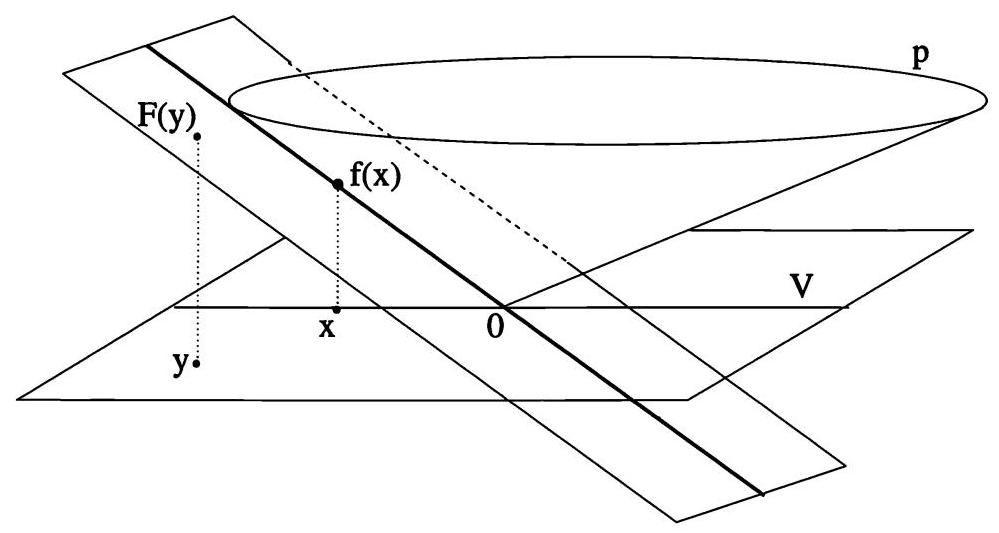
\includegraphics[width=0.9\textwidth]{images/bo_d6ik6nn7aajc739ct1l0_41_242_758_999_533_0.jpg}
\end{center}
\hspace*{3em} 

图2.5.1. 由哈恩-Banach定理，定义在子空间 \(V \subset  X\) 上、且对所有 \(x \in  V\) 满足 \(f\left( x\right)  \leq  p\left( x\right)\) 的线性泛函 \(f : V \mapsto  \mathbb{R}\) ，可延拓为一个线性泛函 \(F : X \mapsto  \mathbb{R}\) ，使得对所有 \(y \in  X\) 均有 \(F\left( y\right)  \leq  p\left( y\right)\) .

前述定理在 \(p\left( x\right)  = \; \| x\|\) 为范数的情形下具有自然应用.

定理2.30(有界线性泛函的延拓定理):设 \(X\) 为实数域或复数域 \(\mathbb{K}\) 上的赋范空间， \(f : V \mapsto  \mathbb{K}\) 为定义在子空间 \(V \subseteq  X\) 上的有界线性泛函，则 \(f\) 可延拓为一个有界线性泛函 \(F : X \mapsto  \mathbb{K}\) ，且保持范数不变:

\[
\| F\|  \doteq  \mathop{\sup }\limits_{{x \in  X,\| x\|  \leq  1}}\left| {F\left( x\right) }\right|  = \mathop{\sup }\limits_{{x \in  V,\| x\|  \leq  1}}\left| {f\left( x\right) }\right|  \doteq  \| f\| .
\]

证明:1. 首先假设 \(\mathbb{K} = \mathbb{R}\) ，即 \(f\) 取实值.令 \(\kappa  \doteq  \| f\|\) ，并定义 \(p\left( x\right)  \doteq  \kappa \| x\|\) .此时结论直接由前述定理得出.

2. 其次考虑 \(\mathbb{K} = \mathbb{C}\) 为复数域的情形.注意此时 \(V\) 与 \(X\) 亦可视为实数域上的向量空间.泛函 \(F : X \mapsto  \mathbb{C}\) 将通过分别构造其实部与虚部而得到.

对于 \(x \in  V\) ，定义 \(u\left( x\right)  \doteq  \operatorname{Re}f\left( x\right)\) .这是 \(V\) 上的一个实值线性泛函，其范数为 \(\| u\|  \leq  \kappa  \doteq  \| f\|\) .因此，由前述步骤可知，它存在一个延拓 \(U : X \mapsto  \mathbb{R}\) ，且范数为 \(\| U\|  \leq  \kappa\) .我们声称该映射

\[
F\left( x\right)  \doteq  U\left( x\right)  - {iU}\left( {ix}\right)
\]

满足全部要求.事实上，对任意 \(x \in  V\) ，

\[
F\left( x\right)  = \operatorname{Re}f\left( x\right)  - i\operatorname{Re}f\left( {ix}\right)  = \operatorname{Re}f\left( x\right)  + i\operatorname{Im}f\left( x\right)  = f\left( x\right) .
\]

此外，设 \(\alpha  \in  \mathbb{C}\) 满足 \(\left| \alpha \right|  = 1,{\alpha F}\left( x\right)  = \left| {F\left( x\right) }\right|\) .则

\[
\left| {F\left( x\right) }\right|  = {\alpha F}\left( x\right)  = U\left( {\alpha x}\right)  \leq  \kappa \| {\alpha x}\|  = \kappa \| x\| .
\]

故 \(\| F\|  \leq  \kappa  \doteq  \| f\|\) .

推论 2.31.设 \(X\) 为 Banach 空间.对任意两个向量 \(x,y \in  X\) ，若 \(x \neq  y\) ，则存在连续线性泛函 \(\phi  : X \mapsto  \mathbb{K}\) ，使得 \(\phi \left( x\right)  \neq  \phi \left( y\right)\) .

推论 2.32.设 \(X\) 为 Banach 空间.对任意向量 \(x \in  X\) ，存在连续线性泛函 \(\phi  : X \mapsto  \mathbb{K}\) ，使得 \(\phi \left( x\right)  = \| x\|\) 且 \(\| \phi \|  = 1.\) .

\begin{center}
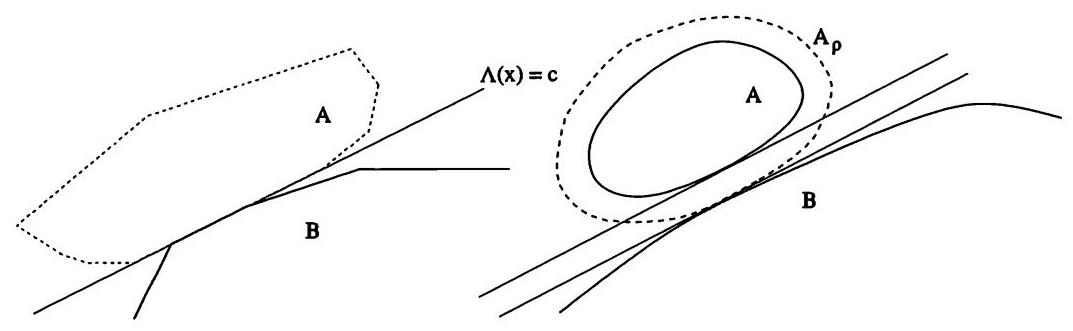
\includegraphics[width=1.0\textwidth]{images/bo_d6ik6nn7aajc739ct1l0_42_203_1420_1073_331_0.jpg}
\end{center}
\hspace*{3em} 

图 2.5.2.左:若 \(A\) 是开集，则不相交的凸集 \(A,B\) 可被一超平面分离.右:若 \(A\) 是紧集且 \(B\) 是闭集，则不相交的凸集 \(A,B\) 可被严格分离.

\section*{2.6. 凸集的分离}

考虑如下问题:给定赋范空间 \(X\) 中两个不相交的凸集 \(A,B\) ，能否找到一个有界线性泛函 \(\phi  : X \mapsto  \mathbb{R}\) ，使得像集 \(\phi \left( A\right)\) 与 \(\phi \left( B\right)\) 不相交？以下定理在 Hahn-Banach 延拓定理基础上给出了肯定回答.

定理 2.33(凸集的分离).设 \(X\) 为实数域上的赋范空间， \(A,B\) 是 \(X\) 中两个非空、不相交的凸子集.

(i) 若 \(A\) 是开集，则存在有界线性泛函 \(\phi  : X \mapsto  \mathbb{R}\) 及某数 \(\mathrm{c} \in  \mathbb{R}\) ，使得

\begin{equation}\tag{2.31}
\phi \left( a\right)  < c \leq  \phi \left( b\right) \;\text{ for all }a \in  A,b \in  B.
\end{equation}

(ii) 若 \(A\) 是紧集且 \(B\) 是闭集，则存在有界线性泛函 \(\phi  : X \mapsto  \mathbb{R}\) 及某些数 \({c}_{1},{c}_{2} \in  \mathbb{R}\) ，使得

\begin{equation}\tag{2.32}
\phi \left( a\right)  \leq  {c}_{1} < {c}_{2} \leq  \phi \left( b\right) \;\text{ for all }a \in  A,b \in  B.
\end{equation}

证明.1. 选取点 \({a}_{0} \in  A\) 与 \({b}_{0} \in  B\) ，并令 \({x}_{0} \doteq  {b}_{0} - {a}_{0}\) .考虑开集

\[
\Omega  \doteq  A - B + {x}_{0} \doteq  \left\{  {\left( {a - {a}_{0}}\right)  + \left( {{b}_{0} - b}\right) ;a \in  A,b \in  B}\right\}  .
\]

由于 \(A,B\) 是凸集且 \(A\) 是开集，显然 \(\Omega\) 是原点的一个开凸邻域.此外， \({x}_{0} \notin  \Omega\) ，否则

\[
{x}_{0} = a - b + {x}_{0},\;a - b = 0,\;\text{ for some }a \in  A,b \in  B.
\]

这与 \(A \cap  B = \varnothing\) 矛盾.

2. 考虑泛函

\begin{equation}\tag{2.33}
p\left( x\right)  \doteq  \inf \{ \lambda  \geq  0;x \in  {\lambda \Omega }\} .
\end{equation}

由于 \(\Omega\) 是原点的一个邻域，故存在某个 \(\rho  > 0\) 使得 \(B\left( {0,\rho }\right)  \subseteq  \Omega\) 成立.因此

\begin{equation}\tag{2.34}
p\left( x\right)  \leq  \frac{\| x\| }{\rho }\;\text{ for all }x \in  X.
\end{equation}

此外， \(\Omega\) 的凸性意味着(2.35)

\(p\left( {x + y}\right)  \leq  p\left( x\right)  + p\left( y\right) ,\;p\left( {tx}\right)  = {tp}\left( x\right) \;\) 对所有 \(x,y \in  X,t \geq  0.\) 成立

注意 \(p\left( {x}_{0}\right)  \geq  1\) ，因为 \({x}_{0} \notin  \Omega\) .

3. 在一维子空间 \(V \doteq  \left\{  {t{x}_{0};t \in  \mathbb{R}}\right\}\) 上，通过设定 \(f\left( {t{x}_{0}}\right)  \doteq  t\) 来定义线性泛函 \(f\) .观察可知

\[
f\left( {x}_{0}\right)  = 1,\;f\left( {t{x}_{0}}\right)  = t \leq  {tp}\left( {x}_{0}\right)  \leq  p\left( {t{x}_{0}}\right) .
\]

由哈恩-Banach延拓定理，存在一个线性泛函 \(\phi  : X \mapsto  \mathbb{R}\) ，使得

\[
- p\left( {-x}\right)  \leq  \phi \left( x\right)  \leq  p\left( x\right) \;\text{ for all }x \in  X.
\]

由(2.34)式显然可知 \(\phi\) 有界.事实上， \(\| \phi \|  \leq  {\rho }^{-1}\) .

4. 若此时 \(a \in  A\) 且 \(b \in  B\) ，则有

\[
\phi \left( a\right)  - \phi \left( b\right)  + 1 = \phi \left( {a - b + {x}_{0}}\right)  \leq  p\left( {a - b + {x}_{0}}\right)  < 1
\]

因为 \(\phi \left( {x}_{0}\right)  = f\left( {x}_{0}\right)  = 1\) ，而 \(a - b + {x}_{0} \in  \Omega\) 且 \(\Omega\) 是开集.因此

\[
\phi \left( a\right)  < \phi \left( b\right) \;\text{ for all }a \in  A,b \in  B.
\]

\(\phi \left( A\right)\) 与 \(\phi \left( B\right)\) 是 \(\mathbb{R}\) 中两个非空、不相交的凸集，且 \(\phi \left( A\right)\) 为开集.取 \(c \doteq  \mathop{\sup }\limits_{{a \in  A}}\phi \left( a\right)\) ，则结论(2.31)成立.这证明了(i).

5. 为证明(ii)，注意到关于 \(A,B\) 的假设意味着

\[
d\left( {A,B}\right)  \doteq  \inf \{ \| a - b\| ;a \in  A,b \in  B\}  > 0.
\]

若选取 \(\rho  \doteq  d\left( {A,B}\right)\) ，则以 \(A\) 为中心、半径为 \(\rho\) 的开邻域 \({A}_{\rho } \doteq  \{ x \in \; X;d\left( {x,A}\right)  < \rho \}\) 不与 \(B\) 相交.因此可将(i)应用于不相交凸集 \({A}_{\rho }\) 与 \(B\) ，从而得到一个连续线性泛函 \(\phi  : X \mapsto  \mathbb{R}\) 及一个常数 \({c}_{2}\) ，使得

\[
\phi \left( x\right)  < {c}_{2} \leq  \phi \left( y\right) \;\text{ for all }x \in  {A}_{\rho },y \in  B.
\]

我们进一步注意到，集合 \(\phi \left( A\right)\) 是紧的，因其为连续映射下紧集的像.故 \({c}_{1} \doteq  \mathop{\sup }\limits_{{x \in  A}}\phi \left( x\right)  < {c}_{2}\) .这完成了(ii)的证明.

\begin{center}
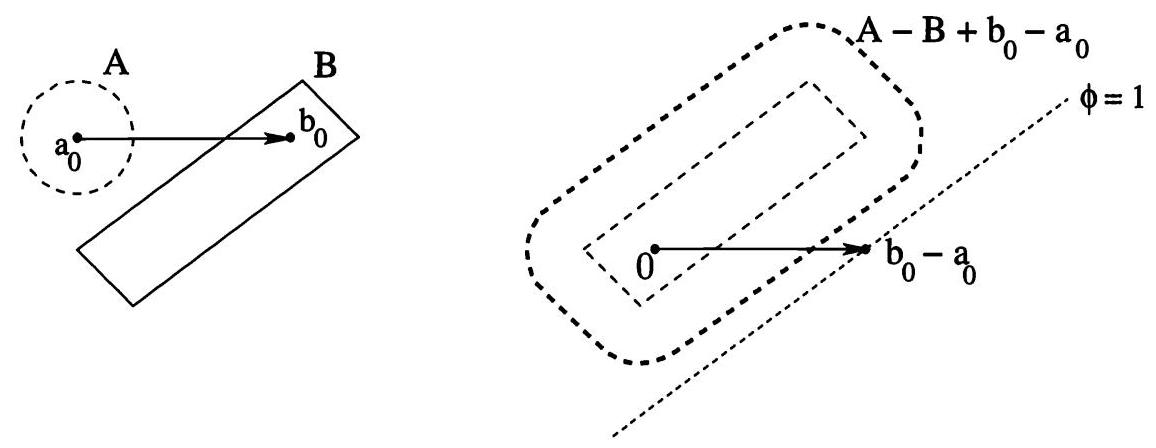
\includegraphics[width=1.0\textwidth]{images/bo_d6ik6nn7aajc739ct1l0_44_155_1289_1156_448_0.jpg}
\end{center}
\hspace*{3em} 

图2.6.1. 分离定理证明中所用的构造.

\section*{2.7. 对偶空间与弱收敛}

设 \(X\) 为实数域或复数域 \(\mathbb{K}\) 上的Banach空间.所有连续线性泛函 \(\varphi  : X \mapsto  \mathbb{K}\) 构成的集合称为 \(X\) 的对偶空间，记作 \({X}^{ * }\) .

注意，线性泛函 \(\varphi  : X \mapsto  \mathbb{K}\) 可视为一种线性算子 \(\varphi  : X \mapsto  Y\) ，特例为 \(Y = \mathbb{K}\) 时.因此我们可以使用

定理2.12，并得出 \({X}^{ * } = \mathcal{B}\left( {X,\mathbb{K}}\right)\) 是一个赋范空间，其范数为

\begin{equation}\tag{2.36}
\| \varphi {\| }_{ * } \doteq  \mathop{\sup }\limits_{{\| x\|  \leq  1}}\left| {\varphi \left( x\right) }\right| .
\end{equation}

2.7.1 弱收敛.Banach空间 \(X\) 中的一列 \({x}_{1},{x}_{2},\ldots\) 称为弱收敛的，若存在 \(x \in  X\) 使得

\[
\mathop{\lim }\limits_{{n \rightarrow  \infty }}\varphi \left( {x}_{n}\right)  = \varphi \left( x\right) \;\text{ for all }\varphi  \in  {X}^{ * }.
\]

此时，称 \(x\) 为序列 \({x}_{n}\) 的弱极限，并记作 \({x}_{n} \rightharpoonup  x\) .我们回顾:序列 \({x}_{n}\) 强收敛于 \(x\) 当且仅当 \(\begin{Vmatrix}{{x}_{n} - x}\end{Vmatrix} \rightarrow\) →0.由于按定义每个 \(\varphi  \in  {X}^{ * }\) 都是连续的，故强收敛 \({x}_{n} \rightarrow  x\) 显然蕴含弱收敛 \({x}_{n} \rightharpoonup  x\) .

若弱极限存在，则必唯一: \({x}_{n} \rightharpoonup  x\) 与 \({x}_{n} \rightharpoonup  y\) 蕴含 \(x = y\) .事实上，假设 \(y \neq  x\) .则由推论2.31，存在连续线性泛函 \(\phi  \in  {X}^{ * }\) 使得 \(\phi \left( x\right)  \neq  \phi \left( y\right)\) .这导致矛盾，因为

\[
\phi \left( x\right)  = \mathop{\lim }\limits_{{n \rightarrow  \infty }}\phi \left( {x}_{n}\right)  = \phi \left( y\right) .
\]

2.7.2 弱*收敛.可换一视角观察:每个向量 \(x \in  X\) 在 \({X}^{ * }\) 上确定一个线性泛函，即

\begin{equation}\tag{2.37}
\varphi  \mapsto  \varphi \left( x\right) ,\;\varphi  \in  {X}^{ * }.
\end{equation}

由推论2.32，该泛函的范数为

\begin{equation}\tag{2.38}
\| x{\| }_{* * } \doteq  \mathop{\sup }\limits_{{\| \varphi {\| }_{ * } \leq  1}}\left| {\varphi \left( x\right) }\right|  = \| x\| .
\end{equation}

于是我们得到标准嵌入 \(\iota  : X \mapsto  {\left( {X}^{ * }\right) }^{ * }\) :对每个元素 \(x \in  X\) ，对应一个定义在对偶空间 \({X}^{ * }\) 上的有界线性泛函 \(\iota \left( x\right)\) ，即映射 \(\varphi  \mapsto  \varphi \left( x\right)\) .由(2.38)可知，该嵌入是等距的，即保持范数.

若 \({X}^{ * }\) 上每个有界线性泛函均可表为(2.37)的形式(对某个 \(x \in  X\) )，则 \(\iota \left( X\right)  = {\left( {X}^{ * }\right) }^{ * }\) ，此时称空间 \(X\) 是自反的.自反空间的例子包括所有有限维空间，以及例2.5与例2.6中的空间 \({\mathbf{L}}^{p}\left( \Omega \right) ,{\ell }^{p}\) ，其中 \(1 < p < \infty\) .

须注意，一般情况下，空间 \({\left( {X}^{ * }\right) }^{ * }\) 可能严格大于 \(\iota \left( X\right)\) .非自反空间的例子包括空间 \({\mathbf{L}}^{1}\left( \Omega \right) ,{\mathbf{L}}^{\infty }\left( \Omega \right) ,{\ell }^{1}\) 与 \({\ell }^{\infty }\) .

嵌入 \(\iota  : X \mapsto  {\left( {X}^{ * }\right) }^{ * }\) 可用于在对偶空间 \({X}^{ * }\) 上引入弱*拓扑.我们称一列有界线性泛函 \({\varphi }_{n} \in  {X}^{ * }\) 弱*收敛于 \(\varphi  \in  {X}^{ * }\) ，并记作 \({\varphi }_{n} \rightarrow  \varphi\) ，若

\begin{equation}\tag{2.39}
\mathop{\lim }\limits_{{n \rightarrow  \infty }}{\varphi }_{n}\left( x\right)  = \varphi \left( x\right) \;\text{ for every }x \in  X.
\end{equation}

这比按范数收敛 \({\varphi }_{n} \rightarrow  \varphi\) 弱得多.事实上

\({\varphi }_{n}\overset{ * }{ \rightharpoonup  }\varphi \;\) 表示对每个 \(x \in  X, \; {\varphi }_{n} \rightarrow  \varphi \;\) ，有 \(\;\left| {{\varphi }_{n}\left( x\right)  - \varphi \left( x\right) }\right|  \rightarrow  0\;\) ； \(\;\mathop{\sup }\limits_{{x \in  X,\| x\|  \leq  1}}\left| {{\varphi }_{n}\left( x\right)  - \varphi \left( x\right) }\right|  \rightarrow  0.\)

由定理2.22可知，若空间 \({X}^{ * }\) 是无限维的，则闭单位球 \({B}_{1} \subset  {X}^{ * }\) 不是紧集:可找到一族线性泛函 \({\varphi }_{n} \in  {X}^{ * }\) ，满足对每个 \(n \geq  1\) 均有 \({\begin{Vmatrix}{\varphi }_{n}\end{Vmatrix}}_{ * } \leq  1\) ，但其中不存在任何(关于 \({X}^{ * }\) 的范数拓扑)收敛子列.另一方面，若将强收敛改为仅要求弱*收敛，则可得到肯定结果.

定理2.34(Banach-Alaoglu定理).设 \(X\) 为可分Banach空间.则任意有界线性泛函序列 \({\varphi }_{n} \in  {X}^{ * }\) 均存在弱*收敛子列.\footnote{Banach-Alaoglu定理即使在不假设 \(X\) 可分的情况下仍成立.对此更一般情形的证明，参见 \(\left\lbrack  {\mathbf{C},\mathbf{R}}\right\rbrack\) .}

证明.1. 考虑有界线性泛函序列 \({\varphi }_{n} \in  {X}^{ * }\) ，例如对所有 \(n \geq  1\) 均有 \({\begin{Vmatrix}{\varphi }_{n}\end{Vmatrix}}_{ * } \leq  C\) .由于 \(X\) 可分，故存在一个可数稠密子集 \(S = \left\{  {{x}_{1},{x}_{2},\ldots }\right\}   \subset  X\) .

2. 我们断言存在一个子列 \({\left( {\varphi }_{{n}_{j}}\right) }_{j \geq  1}\) ，它在每一点 \({x}_{k}\) 处点态收敛，即

\begin{equation}\tag{2.40}
\mathop{\lim }\limits_{{j \rightarrow  \infty }}{\varphi }_{{n}_{j}}\left( {x}_{k}\right)  = \varphi \left( {x}_{k}\right)
\end{equation}

对某些值 \(\varphi \left( {x}_{k}\right)\) 及所有 \(k \geq  1\) 成立.该子列将通过标准对角化方法构造.

由于数列 \({\left( {\varphi }_{n}\left( {x}_{1}\right) \right) }_{n \geq  1}\) 有界，故存在一个无穷指标集 \({I}_{1} \subset  \mathbb{N}\) ，使得子列 \({\left( {\varphi }_{n}\left( {x}_{1}\right) \right) }_{n \in  {I}_{1}}\) 收敛于某个极限 \(\varphi \left( {x}_{1}\right)\) .

类似地，数列 \({\left( {\varphi }_{n}\left( {x}_{2}\right) \right) }_{n \geq  1}\) 亦有界.因此存在一个无穷指标集 \({I}_{2} \subset  {I}_{1}\) ，使得子列 \({\left( {\varphi }_{n}\left( {x}_{2}\right) \right) }_{n \in  {I}_{2}}\) 收敛于某个极限 \(\varphi \left( {x}_{2}\right)\) .

由归纳法，对每个 \(k\) ，存在一个无限指标集 \({I}_{k} \subset  {I}_{k - 1}\) ，使得子列 \({\left( {\varphi }_{n}\left( {x}_{k}\right) \right) }_{n \in  {I}_{k}}\) 收敛于某个极限 \(\varphi \left( {x}_{k}\right)\) .

现选取子列 \({n}_{1} < {n}_{2} < {n}_{3} < \cdots\) ，满足对每个 \(j\) 均有 \({n}_{j} \in  {I}_{j}\) .由于 \(j \rightarrow  \infty\) ，由此得到对每个 \(k \geq  1\) 均有收敛性 \({\varphi }_{{n}_{j}}\left( {x}_{k}\right)  \rightarrow  \varphi \left( {x}_{k}\right)\) .

3. 我们声称极限函数 \(\varphi  : S \mapsto  \mathbb{K}\) 是Lipschitz连续的，其Lipschitz常数为 \(C = \mathop{\sup }\limits_{n}{\begin{Vmatrix}{\varphi }_{n}\end{Vmatrix}}_{ * }\) .事实上，对每个 \({x}_{h},{x}_{k} \in  S\) ，有

\[
\left| {\varphi \left( {x}_{h}\right)  - \varphi \left( {x}_{k}\right) }\right|  = \mathop{\lim }\limits_{{j \rightarrow  \infty }}\left| {{\varphi }_{{n}_{j}}\left( {x}_{h}\right)  - {\varphi }_{{n}_{j}}\left( {x}_{k}\right) }\right|
\]

\[
\leq  \mathop{\limsup }\limits_{{j \rightarrow  \infty }}{\begin{Vmatrix}{\varphi }_{{n}_{j}}\end{Vmatrix}}_{ * }\begin{Vmatrix}{{x}_{h} - {x}_{k}}\end{Vmatrix} \leq  C\begin{Vmatrix}{{x}_{h} - {x}_{k}}\end{Vmatrix}.
\]

因此，映射 \(\varphi\) 可通过连续性唯一延拓至 \(S\) 的闭包，即整个空间 \(X\) .该连续延拓仍记为 \(\varphi  : X \mapsto  \mathbb{K}\) .

4. 剩余需证子列 \({\varphi }_{{n}_{j}}\) 弱*收敛于 \(\varphi\) .任给 \(x \in  X\) 与 \(\varepsilon  > 0\) .由于 \(S\) 稠密，可选取一点 \({x}_{k} \in  S\) 使得 \(\begin{Vmatrix}{{x}_{k} - x}\end{Vmatrix} < \varepsilon\) .注意到所有函数 \({\varphi }_{n}\) 与 \(\varphi\) 均为Lipschitz连续，且Lipschitz常数均为 \(C\) ，故有

\[
\mathop{\limsup }\limits_{{j \rightarrow  \infty }}\left| {{\varphi }_{{n}_{j}}\left( x\right)  - \varphi \left( x\right) }\right|
\]

\[
\leq  \mathop{\limsup }\limits_{{j \rightarrow  \infty }}\left| {{\varphi }_{{n}_{j}}\left( x\right)  - {\varphi }_{{n}_{j}}\left( {x}_{k}\right) }\right|
\]

\[
+ \mathop{\limsup }\limits_{{j \rightarrow  \infty }}\left| {{\varphi }_{{n}_{j}}\left( {x}_{k}\right)  - \varphi \left( {x}_{k}\right) }\right|  + \left| {\varphi \left( {x}_{k}\right)  - \varphi \left( x\right) }\right|
\]

\[
\leq  C\begin{Vmatrix}{x - {x}_{k}}\end{Vmatrix} + 0 + C\begin{Vmatrix}{{x}_{k} - x}\end{Vmatrix} \leq  {2C\varepsilon }.
\]

由于 \(\varepsilon  > 0\) 是任意的，这表明当 \(j \rightarrow  \infty\) 时 \(\left| {{\varphi }_{{n}_{j}}\left( x\right)  - \varphi \left( x\right) }\right|  \rightarrow  0\) ，从而证得弱*收敛 \({\varphi }_{{n}_{j}}\overset{ * }{ \rightharpoonup  }\varphi\) .

作为一致有界线性泛函序列的逐点极限，显然映射 \(\varphi\) 本身也是有界且线性的.

\section*{2.8. 习题}

1. 判断下列集合是否为赋范空间.若否，指出哪个性质(N1)-(N3)不成立；若是，进一步判断其是否为Banach空间.

(i) 设 \(X = \mathbb{R}\) ，其中

\[
\| x\|  = \begin{cases} x & \text{ if }x \geq  0, \\   - {2x} & \text{ if }x < 0. \end{cases}
\]

(ii) 设 \(X\) 为实数列 \(x = \left( {{x}_{1},{x}_{2},{x}_{3},\ldots }\right)\) 构成的向量空间，其中除有限个 \(k\) 外均有 \({x}_{k} = 0\) .在 \(X\) 上取范数(2.8).

(iii) 设 \(X\) 为所有多项式(任意次数)构成的空间，其范数为 \(\| p\|  = \; \mathop{\max }\limits_{{x \in  \left\lbrack  {0,1}\right\rbrack  }}\left| {p\left( x\right) }\right|\) .

(iv) 设 \(X\) 为所有次数为 \(\leq  2\) 的多项式构成的空间，其范数为

\[
\| p\|  \doteq  \left| {p\left( 0\right) }\right|  + \left| {{p}^{\prime }\left( 0\right) }\right|  + \left| {{p}^{\prime \prime }\left( 0\right) }\right| .
\]

(v) 设 \(X\) 为区间 \(\left\lbrack  {0,1}\right\rbrack\) 上所有连续函数构成的空间，其中

\[
\| f\|  \doteq  {\int }_{0}^{1}\left| {f\left( x\right) }\right| {dx}
\]

(vi) 固定 \(\kappa  \in  \mathbb{R}\) ，并令 \(X\) 为所有满足以下条件的连续函数 \(f : \lbrack 0,\infty \lbrack  \mapsto  \mathbb{R}\) 构成的空间:

\[
\| f\|  \doteq  \mathop{\sup }\limits_{{t \geq  0}}{e}^{\kappa t}\left| {f\left( t\right) }\right|  < \infty .
\]

(vii) 设 \(X = {\mathbb{R}}^{2}\) .给定 \(x = \left( {{x}_{1},{x}_{2}}\right)\) ，对固定的 \(0 < p < 1\) ，定义

\[
\| x\|  \doteq  {\left( {\left| {x}_{1}\right| }^{p} + {\left| {x}_{2}\right| }^{p}\right) }^{1/p}.
\]

注:关于 (vii)，值得检验的是

\[
d\left( {x,y}\right)  \doteq  {\left| {x}_{1} - {y}_{1}\right| }^{1/2} + {\left| {x}_{2} - {y}_{2}\right| }^{1/2}
\]

是否为 \({\mathbb{R}}^{2}\) 上的一个距离.开球 \(B\left( {x,r}\right)  = \{ y;d\left( {y,x}\right)  < r\}\) 是否为凸集？ \(d\left( {\cdot , \cdot  }\right)\) 是否平移不变？

2. 设 \(X,Y\) 为 Banach 空间.证明其笛卡尔积

\[
X \times  Y = \{ \left( {x,y}\right) ;x \in  X,y \in  Y\}
\]

在范数

\begin{equation}\tag{2.41}
\| \left( {x,y}\right) \|  \doteq  \max \{ \| x\| ,\| y\| \} .
\end{equation}

3. 设 \(X\) 为实数域或复数域 \(\mathbb{K}\) 上的 Banach 空间.注意: \(X \times  X\) 和 \(\mathbb{K} \times  X\) 均为 Banach 空间，其乘积范数如 (2.41) 所示.证明:

(i) 映射 \(\left( {x,y}\right)  \mapsto  x + y\) 从 \(X \times  X\) 到 \(X\) 是连续的.

(ii) 映射 \(\left( {\alpha ,x}\right)  \mapsto  {\alpha x}\) 从 \(\mathbb{K} \times  X\) 到 \(X\) 是连续的.

4. 设 \(X\) 为具有范数 \(\|  \cdot  \|\) 的赋范空间.证明:任一子空间 \(V \subset  X\) 在同一范数下也构成赋范空间.若 \(X\) 是 Banach 空间且 \(V\) 是闭的，则 \(V\) 也是 Banach 空间.

5. 证明:赋范空间 \(X\) 完备当且仅当每个绝对收敛级数均有和:

\[
\mathop{\sum }\limits_{{k \geq  1}}\begin{Vmatrix}{x}_{k}\end{Vmatrix} < \infty \;\text{ implies that }\;\mathop{\sum }\limits_{{k \geq  1}}{x}_{k} \doteq  \mathop{\lim }\limits_{{n \rightarrow  \infty }}\mathop{\sum }\limits_{{k = 1}}^{n}{x}_{k}\;\text{ exists. }
\]

6. 设 \(X\) 为向量空间.集合 \(A \subset  X\) 的凸包定义为 \(A\) 中元素的所有凸组合构成的集合，即

\[
\operatorname{co}A \doteq  \left\{  {\mathop{\sum }\limits_{{k = 1}}^{N}{\theta }_{k}{a}_{k};N \geq  1,{a}_{k} \in  A,{\theta }_{k} \in  \left\lbrack  {0,1}\right\rbrack  ,\mathop{\sum }\limits_{{k = 1}}^{N}{\theta }_{k} = 1}\right\}  .
\]

证明:(i) \(\operatorname{co}A\) 是凸集；(ii) \(\operatorname{co}A\) 是所有包含 \(A\) 的凸集的交集.

7. 设 \(X\) 为 Banach 空间，且 \(A,B \subset  X\) .证明下列命题.

(i) 若 \(A\) 是开集，则 \(\operatorname{co}A\) 也是开集.

(ii) 若 \(A\) 是有界集，则 co \(A\) 也是有界集.

(iii) 若 \(A,B\) 是有界集，则集合 \(A + B \doteq  \{ a + b;a \in  A,b \in  B\}\) 也是有界集.

(iv) 若 \(A\) 是闭集且 \(B\) 是紧集，则 \(A + B\) 是闭集.

(v) 两个闭集的和未必是闭集.

(vi) 若 \(A\) 是凸集，则 \(A + A \doteq  \{ x + y;x \in  A,y \in  A\}  = {2A} \doteq  \{ {2x};x \in  A\}\) .

(vii) 若 \(A\) 是闭集且 \(A + A = {2A}\) ，则 \(A\) 必为凸集.

8. 设 \(X\) 是赋范空间.若集合 \(S \subseteq  X\) 满足 \(a \in  S\) 蕴含 \(- a \in  S\) ，则称其为对称集.证明:

(i) 若 \(S\) 是凸集，则其闭包也是凸集.

(ii) 若 \(S\) 是对称集，则其闭包也是对称集.

9. 设 \(X,Y\) 是实数域上的Banach空间， \(\Lambda  : X \mapsto  Y\) 是有界线性算子.证明:

(i) 若 \(S\) 是凸集，则其像 \(\Lambda \left( S\right)\) 是凸集.

(ii) 若 \(S\) 是对称集，则其像 \(\Lambda \left( S\right)\) 是对称集.

10. 设 \(\Lambda  : X \mapsto  Y\) 是线性算子.假设对任一序列 \({x}_{n} \rightarrow  0\) ，序列 \({\left( \Lambda {x}_{n}\right) }_{n \geq  1}\) 均有界.证明: \(\Lambda\) 是连续的.

11. 设 \(X\) 是无限维Banach空间， \(S\) 是一组线性无关向量.记 span \(\left( S\right)\) 为 \(S\) 中元素的所有(有限)线性组合构成的集合.证明:

(i) 若 \(S = \left\{  {{v}_{1},\ldots ,{v}_{N}}\right\}\) 是有限集，则 \(\operatorname{span}\left( S\right)\) 是 \(X\) 的闭子空间.

(ii) 若 \(S = \left\{  {{v}_{k};k \geq  1}\right\}\) 为无穷序列，则向量空间span \(\left( S\right)\) 在 \(X\) 中不可能是闭的.

12(实数域与复数域上的空间).设 \(X\) 为复数域上的向量空间，则 \(X\) 亦为实数域上的向量空间.若 \(\Phi  : X \mapsto  \mathbb{C}\) 为复线性泛函， \(\phi \left( x\right)  = \operatorname{Re}\Phi \left( x\right)\) 为其实部，证明 \(\phi\) 为实线性泛函，且 \(\Phi \left( x\right)\) 可由 \(\phi\) 按如下方式重构:

\[
\Phi \left( x\right)  = \phi \left( x\right)  - {i\phi }\left( {ix}\right) .
\]

13. 证明赋范空间 \(X\) 是有限维的当且仅当其对偶空间 \({X}^{ * }\) 是有限维的.

14. 考虑例2.6与2.7中定义的实数序列空间 \({\ell }^{p}\) .若 \(1 \leq  p \leq  q \leq  \infty\) ，则 \({\ell }^{p} \subseteq  {\ell }^{q}\) ，且等号成立当且仅当 \(p = q\) .此外，证明恒等算子 \(\Lambda  : {\ell }^{p} \mapsto  {\ell }^{q}\) (定义为 \(\Lambda \mathbf{x} = \mathbf{x}\) )对每个 \(p \leq  q\) 均连续.

15. 对 \(1 \leq  p < \infty\) ，证明(2.10)中引入的子空间 \(V \doteq  \operatorname{span}\left\{  {{\mathbf{e}}_{k};k \geq  1}\right\}\) 在空间 \({\ell }^{p}\) 中稠密.对 \(p = \infty\) ，证明 \(V\) 的闭包恰为所有收敛于零的序列构成的子空间 \({c}_{0}\) .

16.(对角算子的性质)对 \(1 \leq  p \leq  \infty\) ，考虑(2.13)中定义的算子 \(\Lambda  : {\ell }^{p} \mapsto  {\ell }^{p}\) .证明例2.14中(i)-(ii)项断言.

17. 补全例2.18的细节:即固定 \(1 \leq  p \leq  \infty\) ，并设 \(g : \Omega  \mapsto  \mathbb{R}\) 为任意可测函数.

(i) 若 \(g \in  {\mathbf{L}}^{\infty }\left( \Omega \right)\) ，证明乘法算子 \({M}_{g} : f \mapsto  {gf}\) 从 \({\mathbf{L}}^{p}\left( \Omega \right)\) 到自身的映射是有界的，且其范数由(2.15)给出.

(ii) 若 \(g \notin  {\mathbf{L}}^{\infty }\left( \Omega \right)\) ，证明线性算子 \(f \mapsto  {gf}\) 从 \({\mathbf{L}}^{p}\left( \Omega \right)\) 到自身的映射是无界的.直接证明 \(\operatorname{Dom}\left( {M}_{g}\right)  \neq  {\mathbf{L}}^{p}\left( \Omega \right)\) .

18. 固定 \(1 \leq  p \leq  \infty\) .设 \({\left( {f}_{n}\right) }_{n \geq  1}\) 为 \({\mathbf{L}}^{p}\left( \mathbb{R}\right)\) 中一列弱收敛于函数 \(f \in  {\mathbf{L}}^{p}\left( \mathbb{R}\right)\) 的函数.证明:

\[
\mathop{\lim }\limits_{{n \rightarrow  \infty }}{\int }_{a}^{b}{f}_{n}\left( x\right) {dx} = {\int }_{a}^{b}f\left( x\right) {dx}\;\text{ for all }a < b.
\]

19. 考虑下列函数序列

\[
{f}_{n}\left( x\right)  = \left\{  \begin{matrix} 1/n & & \text{ if }x \in  \left\lbrack  {0,n}\right\rbrack  , \\  0 & & \text{ otherwise. } \end{matrix}\right.
\]

(i) 证明: \({f}_{n} \rightarrow  0\) 在每个满足 \(1 < p \leq  \infty\) 的空间 \({\mathbf{L}}^{p}\left( \mathbb{R}\right)\) 中强收敛(即 \(\begin{Vmatrix}{f}_{n}\end{Vmatrix} \rightarrow  0\) ).

(ii) 另一方面，证明:在空间 \({\mathbf{L}}^{1}\left( \mathbb{R}\right)\) 中，该序列不强收敛；事实上，该序列甚至不存在任何弱收敛子列.

20. 设 \(Y\) 是 Banach 空间 \(X\) 的子空间， \(\Lambda  : Y \mapsto  {\mathbb{R}}^{n}\) 是从 \(Y\) 到欧氏空间 \({\mathbb{R}}^{n}\) 的有界线性算子.证明: \(\Lambda\) 可延拓为一线性算子 \(\widetilde{\Lambda } : X \mapsto  {\mathbb{R}}^{n}\) ，其范数为 \(\| \widetilde{\Lambda }\|  \leq  \sqrt{n}\| \Lambda \|\) .

21. 设 \(\phi  : {\mathbb{R}}^{2} \mapsto  \mathbb{R}\) 是一线性泛函，记为 \(\phi \left( {{x}_{1},{x}_{2}}\right)  = a{x}_{1} + b{x}_{2}\) .给出如下结论的直接证明:

(i) 若 \({\mathbb{R}}^{2}\) 赋以范数 \(\| x{\| }_{1} = \left| {x}_{1}\right|  + \left| {x}_{2}\right|\) ，则相应算子范数(2.36)为 \(\| \phi {\| }_{\infty } = \max \{ \left| a\right| ,\left| b\right| \}\) .

(ii) 若 \({\mathbb{R}}^{2}\) 赋以范数 \(\| x{\| }_{\infty } = \max \left\{  {\left| {x}_{1}\right| ,\left| {x}_{2}\right| }\right\}\) ，则相应范数(2.36)为 \(\| \phi {\| }_{1} = \left| a\right|  + \left| b\right|\) .

(iii) 若 \({\mathbb{R}}^{2}\) 赋以范数 \(\| x{\| }_{p} = {\left( {\left| {x}_{1}\right| }^{p} + {\left| {x}_{2}\right| }^{p}\right) }^{1/p}\) ，其中 \(1 < p < \; \infty\) ，则相应范数(2.36)为 \(\| \phi {\| }_{q} = {\left( {\left| a\right| }^{q} + {\left| b\right| }^{q}\right) }^{1/q}\) ，其中 \(\frac{1}{p} + \frac{1}{q} = 1\)

22. 设 \(X\) 是一矢量空间， \(B \subset  X\) 是其凸子集，且对任一非零向量 \(x \in  X\) ，均存在正数 \({\theta }_{x} > 0\) ，使得

\({\alpha x} \in  B\) 当且仅当 \(\left| \alpha \right|  \leq  {\theta }_{x}.\)

对 \(r \geq  0\) ，记 \({rB} \doteq  \{ {rb};b \in  B\}\) .证明:

\[
\| x\|  \doteq  \min \{ r \geq  0;x \in  {rB}\}
\]

是 \(X\) 上的一个范数，且 \(B = \{ x \in  X;\| x\|  \leq  1\}\) 是该范数下的单位球.

23. 设 \(\Omega  \subseteq  {\mathbb{R}}^{n}\) 为开集.在(可能无界)连续函数 \(f : \Omega  \mapsto  \mathbb{R}\) 的空间 \(\mathcal{C}\left( \Omega \right)\) 上，考虑半范数 \({p}_{k}\left( \cdot \right)\) 和在 (2.22)、(2.20) 中定义的距离 \(d\left( {\cdot , \cdot  }\right)\) .

接下来，考虑任意一列开集 \({A}_{k}^{\prime }\) ，其紧致地包含于 \(\Omega\) 中，且满足 \(\mathop{\bigcup }\limits_{{k > 1}}{A}_{k}^{\prime } = \Omega\) .如前定义半范数 \({p}_{k}^{\prime }\left( \cdot \right)\) 与距离 \({d}^{\prime }\left( {\cdot , \cdot  }\right)\) ，但将(2.21)中的集合 \({A}_{k}\) 替换为集合 \({A}_{k}^{\prime }\) .

证明两个距离 \(d,{d}^{\prime }\) 等价.即:对任意连续函数序列 \({\left( {f}_{j}\right) }_{j \geq  1}\) ，下列命题等价:

(i) 该序列关于距离 \(d\) 是Cauchy列，

(ii) 该序列关于距离 \({d}^{\prime }\) 是Cauchy列，

(iii) 函数 \({f}_{j}\) 在 \(\Omega\) 的每个紧子集上一致收敛.

24. 在空间 \(\mathcal{C}\left( \Omega \right)\) 上，考虑由(2.22)定义的半范数 \({p}_{k}\left( \cdot \right)\) 及由(2.20)构造的距离 \(d\left( {\cdot , \cdot  }\right)\) .

(i) 解释为何 \(\| f\|  \doteq  \mathop{\sum }\limits_{{k = 1}}^{\infty }{2}^{-k}{p}_{k}\left( f\right)\) 不能在 \(\mathcal{C}\left( \Omega \right)\) 上诱导出一个范数.

(ii) 考虑以0(即恒零函数)为中心的开单位球 \(B \doteq  \{ f \in  \mathcal{C}\left( \Omega \right) ;d\left( {f,0}\right)  < 1\}\) .解释为何

\[
\| f{\| }_{\diamond } \doteq  \inf \left\{  {\lambda  > 0;{\lambda }^{-1}f \in  B}\right\}
\]

不能在 \(\mathcal{C}\left( \Omega \right)\) 上诱导出一个范数.

25. 设 \(X\) 为Banach空间.考虑任意集合 \(S \subset  X\) ，并假设 \(x \in  \operatorname{span}\left( S\right)\) .证明存在点 \({x}_{j} \in  S\) 与系数 \({c}_{j} \in  \mathbb{K},j = 1,\ldots ,N\) ，使得

\begin{equation}\tag{2.42}
x = \mathop{\sum }\limits_{{j = 1}}^{N}{c}_{j}{x}_{j},\;\begin{Vmatrix}{\mathop{\sum }\limits_{{j = 1}}^{k}{c}_{j}{x}_{j}}\end{Vmatrix} \leq  2\| x\| \;\text{ for all }k = 1,\ldots ,N.
\end{equation}

26. 设 \(S\) 为Banach空间 \(X\) 的一个子集.证明下列命题等价:

(i) \(x \in  \overline{\operatorname{span}\left( S\right) }\) .

(ii) \(x = \mathop{\sum }\limits_{{j = 1}}^{\infty }{c}_{j}{x}_{j} \doteq  \mathop{\lim }\limits_{{n \rightarrow  \infty }}\mathop{\sum }\limits_{{j = 1}}^{n}{c}_{j}{x}_{j}\) ，其中点 \({x}_{j} \in  S\) 与数 \({c}_{j} \in  \mathbb{K}\) 满足某条件

27. 考虑Banach空间 \({\ell }^{\infty }\) ，其由所有实数有界序列 \(x = \; \left( {{x}_{1},{x}_{2},{x}_{3},\ldots }\right)\) 构成.

(i) 证明存在有界线性泛函 \(F : {\ell }^{\infty } \mapsto  \mathbb{R}\) ，使得

\begin{equation}\tag{2.43}
\left| {F\left( x\right) }\right|  \leq  \| x{\| }_{{\ell }^{\infty }} \doteq  \mathop{\sup }\limits_{{n \geq  1}}\left| {x}_{n}\right|
\end{equation}

\begin{equation}\tag{2.44}
F\left( x\right)  = \mathop{\lim }\limits_{{n \rightarrow  \infty }}{x}_{n}\;\text{ if the limit exists. }
\end{equation}

(ii) 证明:若 \(F : {\ell }^{\infty } \mapsto  \mathbb{R}\) 满足上述性质(2.43)-(2.44)，则

\[
\mathop{\liminf }\limits_{{n \rightarrow  \infty }}{x}_{n} \leq  F\left( x\right)  \leq  \mathop{\limsup }\limits_{{n \rightarrow  \infty }}{x}_{n}\;\text{ for all }x \in  {\ell }^{\infty }.
\]

(iii) 利用(ii)证明:若存在整数 \(N\) ，使得对所有 \(n \geq  N\) 均有 \({x}_{n} \leq  {y}_{n}\) ，则 \(F\left( x\right)  \leq  F\left( y\right)\) .

(iv) 证明:对任意序列 \(a = \left( {{a}_{1},{a}_{2},\ldots }\right)  \in  {\ell }^{1}\) ，该连续线性泛函

\[
{F}_{a}\left( x\right)  \doteq  \mathop{\sum }\limits_{{n \geq  1}}{a}_{n}{x}_{n}
\]

不可能满足(2.44).因此， \({\ell }^{\infty }\) 上所有连续线性泛函构成的空间无法与 \({\ell }^{1}\) 等同.

(v) 对每个有界实数列 \(x = \left( {{x}_{1},{x}_{2},\ldots }\right)\) ，定义

\[
\widetilde{F}\left( x\right)  \doteq  \frac{1}{2}\left( {\mathop{\liminf }\limits_{{n \rightarrow  \infty }}{x}_{n}}\right)  + \frac{1}{2}\left( {\mathop{\limsup }\limits_{{n \rightarrow  \infty }}{x}_{n}}\right) .
\]

\(\widetilde{F}\) 是否满足(2.43)-(2.44)？ \(\widetilde{F}\) 是否为Banach空间 \({\ell }^{\infty }\) 上的有界线性泛函？

28. 在Banach空间 \(X = {\mathbf{L}}^{\infty }\left( \mathbb{R}\right)\) 中，考虑由所有有界连续函数构成的子空间 \(V\) .

证明:存在一个满足 \(\| \Lambda \|  = 1\) 的有界线性泛函 \(\Lambda  : {\mathbf{L}}^{\infty }\left( \mathbb{R}\right)  \mapsto  \mathbb{R}\) ，使得对每个有界连续函数 \(f\) 均有 \({\Lambda f} \doteq  f\left( 0\right)\) .但需指出:不存在函数 \(g \in  {\mathbf{L}}^{1}\left( \mathbb{R}\right)\) ，使得对每个 \(f \in  {\mathbf{L}}^{\infty }\left( \mathbb{R}\right)\) 均有 \({\Lambda f} = \int {fgdx}\) .

由此得出: \({\mathbf{L}}^{\infty }\left( \mathbb{R}\right)\) 的对偶空间无法与 \({\mathbf{L}}^{1}\left( \mathbb{R}\right)\) 等同.

29. 设 \(X\) 为赋范空间， \(\Omega  \subset  X\) 为包含原点的开凸集.考虑泛函

\begin{equation}\tag{2.45}
p\left( x\right)  \doteq  \inf \{ \lambda  \geq  0;x \in  {\lambda \Omega }\} .
\end{equation}

(i) 证明 \(p\left( \cdot \right)\) 满足下列条件

\[
p\left( {x + y}\right)  \leq  p\left( x\right)  + p\left( y\right) ,\;p\left( {tx}\right)  = {tp}\left( x\right) \text{ for all }x,y \in  X,t \geq  0.
\]

(ii) 在假设 \({B}_{r} \doteq  \{ x \in  X;\| x\|  < r\}  \subseteq  \Omega\) 成立的前提下，证明 \(p\left( x\right)  \leq  \| x\| /r\) .

(iii) 在假设 \(\Omega  = \{ x \in  X;\| x\|  < 1\}\) 为开单位球的前提下，证明 \(p\left( x\right)  = \| x\| .\)

30. 设 \({\mathcal{C}}^{0}\left( \left\lbrack  {0,1}\right\rbrack  \right)\) 为定义在 \(\left\lbrack  {0,1}\right\rbrack   \mapsto  \mathbb{R}\) 上的所有实值连续函数 \(f\) 构成的Banach空间，其范数为 \(\| f\|  = \mathop{\max }\limits_{{x \in  \left\lbrack  {0,1}\right\rbrack  }}\left| {f\left( x\right) }\right|\) .

(i) 证明 \(X = \left\{  {f \in  {\mathcal{C}}^{0}\left( \left\lbrack  {0,1}\right\rbrack  \right) ;f\left( 0\right)  = 0}\right\}\) 是 \({\mathcal{C}}^{0}\) 的闭子空间，从而本身亦为Banach空间.

(ii) 证明映射 \(f \mapsto  {\Lambda f} \doteq  {\int }_{0}^{1}f\left( x\right) {dx}\) 是 \(X\) 上的连续线性泛函.计算其范数 \(\| \Lambda \|  \doteq  \mathop{\sup }\limits_{{\| f\|  \leq  1}}\left| {\Lambda f}\right|\) .该上确界是否在闭单位球上实际取到(即是否为最大值)？

31. 设 \(X\) 为实数域上的Banach空间， \({X}^{ * }\) 为其对偶空间.设 \(\Omega  \subset  X\) 为包含原点的凸集.定义

\[
{\Omega }^{ * } \doteq  \left\{  {\phi  \in  {X}^{ * };\phi \left( x\right)  \leq  1\text{ for all }x \in  \Omega }\right\}  ,
\]

\[
{\Omega }^{* * } \doteq  \left\{  {x \in  X;\phi \left( x\right)  \leq  1\text{ for all }\phi  \in  {\Omega }^{ * }}\right\}
\]

证明 \({\Omega }^{* * }\) 是 \(\Omega\) 的闭包.

32. 设 \(\xi\) 为实数域上Banach空间 \(X\) 中的一个非零向量.称 \(U = \; \operatorname{span}\{ \xi \}  = \{ {t\xi };t \in  \mathbb{R}\}\)

证明存在一个闭子空间 \(V \subset  X\) ，使得 \(X = U \oplus  V\) .即，每个元素 \(x \in  X\) 均可唯一地表示为如下和:

\[
x = u + v\;\text{ with }\;u \in  U,v \in  V.
\]

此外，投影算子 \(x \mapsto  u = {\pi }_{U}x\) 和 \(x \mapsto  v = {\pi }_{V}x\) 均为连续线性算子.

33. 在Banach空间 \(X = {\mathbf{L}}^{1}\left( \left\lbrack  {-1,1}\right\rbrack  \right)\) 上，证明存在一个范数为 \(\| \varphi \|  = 1\) 的连续线性泛函 \(\varphi  : X \mapsto  \mathbb{R}\) ，具有如下性质:

\[
\text{ If }f\text{ is a polynomial of degree 1, then }\varphi \left( f\right)  = {f}^{\prime }\left( 0\right) \text{ . }
\]

34. 给定开集 \(\Omega  \subset  {\mathbb{R}}^{n}\) ，记 \({\mathcal{C}}^{m}\left( \Omega \right)\) 为所有具有直至 \(m\) 阶连续偏导数的连续函数 \(f : \Omega  \mapsto  \mathbb{R}\) 构成的空间.设 \({A}_{k}\) 为 (2.21) 中定义的集合.证明半范数序列

\begin{equation}\tag{2.46}
{p}_{k}\left( f\right)  \doteq  \mathop{\sum }\limits_{{\left| \alpha \right|  \leq  m}}\mathop{\max }\limits_{{x \in  {A}_{k}}}\left| {{D}^{\alpha }f\left( x\right) }\right|
\end{equation}

使 \({\mathcal{C}}^{m}\left( \Omega \right)\) 成为Fréchet空间.此处 \(\alpha  = \left( {{\alpha }_{1},\ldots ,{\alpha }_{n}}\right)\) 是长度为 \(\left| \alpha \right|  \doteq  {\alpha }_{1} + \cdots  + {\alpha }_{n}\) 的多重指标，且 \({D}^{\alpha }f \doteq  {\left( \frac{\partial }{\partial {x}_{1}}\right) }^{{\alpha }_{1}}\cdots {\left( \frac{\partial }{\partial {x}_{n}}\right) }^{{\alpha }_{n}}f\) .

35. 设 \(Y\) 为Banach空间 \(X\) 的一个闭子空间，且假设 \({x}_{0} \in  X \setminus  Y\) .证明存在一个有界线性泛函 \(\varphi  \in  {X}^{ * }\) ，使得 \(\| \varphi \|  \leq  1\) 且

\[
\varphi \left( {x}_{0}\right)  = d\left( {{x}_{0},Y}\right)  = \mathop{\inf }\limits_{{y \in  Y}}\begin{Vmatrix}{{x}_{0} - y}\end{Vmatrix},\;\varphi \left( y\right)  = 0\text{ for all }y \in  Y.
\]

36. 在实数列空间 \({\ell }^{p}\) 中，考虑如 (2.9) 所定义的单位向量 \({\mathbf{e}}_{k}\) .证明

(i) 若 \(1 < p < \infty\) ，则序列 \({\left( {\mathbf{e}}_{k}\right) }_{k \geq  1}\) 在 \({\ell }^{p}\) 中弱收敛于零.

(ii) 在空间 \({\ell }^{1}\) 中，序列 \({\left( {\mathbf{e}}_{k}\right) }_{k \geq  1}\) 不含任何弱收敛子列.

37. 设 \(\phi  : \mathbb{R} \mapsto  \mathbb{R}\) 为一光滑且递增的函数，并考虑算子 \(\left( {\Lambda f}\right) \left( x\right)  \doteq  f\left( {\phi \left( x\right) }\right)\) .推导出关于 \(\phi\) 的一个条件，使得 \(\Lambda\) 是从 \({\mathbf{L}}^{p}\left( \mathbb{R}\right)\) 到其自身的有界线性算子.分别讨论 \(1 \leq  p < \infty\) 和 \(p = \infty\) 两种情形.

38. 证明勒贝格测度的概念无法推广到无穷维空间.更准确地说，设 \(X\) 为一无穷维Banach空间.

证明:不存在定义在 \(X\) 的博雷尔子集 σ-代数上的测度 \(\mu\) ，使其满足如下性质:

(i) 对每个非空开集 \(\Omega  \subset  X\) ，均有 \(\mu \left( \Omega \right)  > 0\) ；

(ii) \(\mu\) 是平移不变的:对所有 \(x \in  X\) 和 \(S \subset  X\) ，均有 \(\mu \left( {x + S}\right)  = \mu \left( S\right)\) ；

(iii) 存在一非空开集 \({\Omega }_{0}\) ，使得 \(\mu \left( {\Omega }_{0}\right)  < \infty\) .

39. 设 \(X\) 为一实数域上的Banach空间.

(i) 设 \(S \subset  X\) 为一闭凸集，且假设 \(y \notin  S\) .证明存在一有界线性泛函 \(\varphi  \in  {X}^{ * }\) ，使得

\[
\varphi \left( y\right)  < \mathop{\inf }\limits_{{x \in  S}}\varphi \left( x\right) .
\]

(ii) 考虑一弱收敛序列: \({x}_{n} \rightharpoonup  y\) .令 \(S \doteq  \overline{\operatorname{co}\left\{  {{x}_{n};n \geq  1}\right\}  }\) 为包含所有点 \({x}_{n}\) 的最小闭凸集.证明 \(y \in  S\) .

40. 给定一函数 \(f \in  {\mathbf{L}}^{\infty }\left( \mathbb{R}\right)\) ，我们称

\[
\mathop{\operatorname{ess}}\limits_{{x \rightarrow  0}}\mathop{\lim }\limits_{{f\left( x\right) }}f\left( x\right)  = \lambda
\]

若存在一函数 \(\widetilde{f}\) ，使得对几乎处处的 \(x \in  \mathbb{R}\) 有 \(\widetilde{f}\left( x\right)  = f\left( x\right)\) ，且此外 \(\mathop{\lim }\limits_{{x \rightarrow  0}}\widetilde{f}\left( x\right)  = \lambda\) .

(i) 证明存在一有界线性泛函 \(\Phi  : {\mathbf{L}}^{\infty }\left( \mathbb{R}\right)  \mapsto  \mathbb{R}\) ，使得

\[
\Phi \left( f\right)  = \underset{x \rightarrow  0}{\operatorname{ess}\lim }f\left( x\right)
\]

只要该极限存在.

(ii) 若将空间 \({\mathbf{L}}^{\infty }\left( \mathbb{R}\right)\) 替换为 \({\mathbf{L}}^{1}\left( \mathbb{R}\right)\) ，则上述结论不成立.


\chapter{连续函数空间}

\vspace{-2 em}
\section{有界连续函数}

设 $E$ 是一个度量空间.记 $\mathcal{C}\left( E\right)$ 为所有连续实值(可能无界)函数 $f : E \mapsto  \mathbb{R}$ 构成的空间.一般而言，该空间没有自然范数.因此，我们还将考虑所有有界连续函数 $f : E \mapsto  \mathbb{R}$ 构成的空间 $\mathcal{B}C\left( E\right)$ ，其范数为
\begin{equation}\tag{3.1}\label{eq:bc-norm}
\| f\|  \doteq  \mathop{\sup }\limits_{{x \in  E}}\left| {f\left( x\right) }\right| .
\end{equation}


本章大部分内容将讨论 $E$ 为紧集的情形.此时，每个连续函数 $f : E \mapsto  \mathbb{R}$ 必然有界，故 $\mathcal{C}\left( E\right)  = \mathcal{B}C\left( E\right)$ .

\begin{lemma}\label{lem:bc-banach}
$\mathcal{B}C\left( E\right)$ 是一个Banach空间.
\end{lemma}

\begin{proof}
1. 设 ${\left( {f}_{n}\right) }_{n \geq  1}$ 是 $\mathcal{B}C\left( E\right)$ 中的一个柯西列.则对每个固定的 $x \in  E$ ，数列 ${f}_{n}\left( x\right)$ 是柯西列，因而收敛于某个极限，记为 $f\left( x\right)$ .

2. 由假设，对每个 $\varepsilon  > 0$ ，存在足够大的 $N$ ，使得
\[
\mathop{\sup }\limits_{{x \in  E}}\left| {{f}_{n}\left( x\right)  - {f}_{m}\left( x\right) }\right|  \leq  \varepsilon \;\forall\,n,m \geq  N.
\]

令 $m \rightarrow  \infty$ ，由于 ${f}_{m}\left( x\right)  \rightarrow  f\left( x\right)$ ，得
\[
\mathop{\sup }\limits_{{n \geq  N}}\mathop{\sup }\limits_{{x \in  E}}\left| {{f}_{n}\left( x\right)  - f\left( x\right) }\right|  \leq  \varepsilon .
\]

进而可得
\[
\mathop{\sup }\limits_{{n \geq  N}}\norm{{f}_{n} - f} \leq  \varepsilon ,\;\mathop{\sup }\limits_{{x \in  E}}\left| {f\left( x\right) }\right|  \leq  \varepsilon  + \mathop{\sup }\limits_{{x \in  E}}\left| {{f}_{N}\left( x\right) }\right|  < \infty .
\]
由于$\varepsilon$是任意的，第一个不等式表明 $\norm{{f}_{n} - f} \rightarrow  0$ 收敛；第二个不等式表明 $f$ 有界.

3. 最后，我们证明 $f$ 连续.任给 $x \in  E$ 和 $\varepsilon  > 0$ .由一致收敛性，存在整数 $N$ ，使得对所有 $x \in  E$ 均有 $\left| {{f}_{N}\left( x\right)  - f\left( x\right) }\right|  < \varepsilon /3$ .又因 ${f}_{N}$ 连续，故存在 $\delta  > 0$ ，使得当 $d\left( {y,x}\right)  < \delta$ 时有 $\left| {{f}_{N}\left( y\right)  - {f}_{N}\left( x\right) }\right|  < \varepsilon /3$ .综合上述不等式，当 $d\left( {y,x}\right)  < \delta$ 时，有
{\setjot[-2]\begin{align*}
\left| {f\left( y\right)  - f\left( x\right) }\right|  &\leq  \left| {f\left( y\right)  - {f}_{N}\left( y\right) }\right|  + \left| {{f}_{N}\left( y\right)  - {f}_{N}\left( x\right) }\right|  + \left| {{f}_{N}\left( x\right)  - f\left( x\right) }\right|\\
&< \frac{\varepsilon }{3} + \frac{\varepsilon }{3} + \frac{\varepsilon }{3} = \varepsilon
\end{align*}}

从而证得 $f$ 在点 $x$ 处连续.
\end{proof}

\begin{note}[逐点收敛与一致收敛]\label{rem:pointwise-vs-uniform}
前面的论证表明，如果连续函数序列 ${f}_{n}$一致收敛于函数 $f$ ，那么 $f$ 也是连续的.另一方面，连续函数序列可以逐点收敛到一个不连续的极限.例如，在区间 $E = \left(  {0,1}\right)$ 上，函数序列 ${f}_{n}\left( x\right)  = {x}^{n}$ 逐点收敛到不连续函数
\[
f\left( x\right)  =
\begin{cases}
0, & 0 \leq x < 1,\\
1, & x = 1.
\end{cases}
\]

显然，此处的收敛在整区间 $\left(  {0,1}\right)$ 上并非一致收敛.
\end{note}

以下定理描述了一种逐点收敛蕴含一致收敛的情形.我们回顾:函数列 ${f}_{n} : E \mapsto  \mathbb{R}$ 称为递增的，若 $m < n$ 蕴含 ${f}_{m}\left( x\right)  \leq  {f}_{n}\left( x\right)$ 对所有 $x \in  E$ 成立.

\begin{theorem}[Dini]\label{thm:dini}
设 $E$ 为紧致度量空间.若 ${\left( {f}_{n}\right) }_{n \geq  1}$ 是 $\mathcal{C}\left( E\right)$ 中一列递增函数，且逐点收敛于连续极限函数 $f$ ，则 ${f}_{n} \rightarrow  f$ 在 $E$ 上一致收敛.
\end{theorem}

\begin{proof}
任取$\varepsilon  > 0$，由假设，对每个$x \in  E$，存在整数$N\left( x\right)$，使得$\left| {{f}_{N\left( x\right) }\left( x\right)- f\left( x\right) }\right|  < \varepsilon$.

由于 ${f}_{N\left( x\right) }$ 与 $f$ 连续，存在 $x$ 的一个开邻域 ${V}_{x}$ ，使得对每个 $y \in  {V}_{x}$ ，均有 $\left| {{f}_{N\left( x\right) }\left( y\right)  - {f}_{N\left( x\right) }\left( x\right) }\right|  < \varepsilon$ 且 $\left| {f\left( y\right)  - f\left( x\right) }\right|  < \varepsilon$ .

由于 $E$ 紧致，可用其中有限个此类邻域覆盖 $E$ ，记为 $E \subseteq  {V}_{{x}_{1}} \cup  \cdots  \cup  {V}_{{x}_{m}}$ .

取整数 $N = \max \left\{  {N\left( {x}_{1}\right) ,\ldots ,N\left( {x}_{m}\right) }\right\}$ .\par
对任意 $n \geq  N$ 与 $y \in  E$ ，若假设 $y \in  {V}_{{x}_{i}}$，则有
\[
{f}_{N\left( {x}_{i}\right) }\left( y\right)  \leq  {f}_{N}\left( y\right)  \leq  {f}_{n}\left( y\right)  \leq  f\left( y\right) ,
\]

因为该序列递增.故
{\setjot[-2]\begin{align*}
\left| {{f}_{n}\left( y\right)  - f\left( y\right) }\right|  &\leq  \left| {{f}_{N\left( {x}_{i}\right) }\left( y\right)  - f\left( y\right) }\right| \\
&\leq  \left| {{f}_{N\left( {x}_{i}\right) }\left( y\right)  - {f}_{N\left( {x}_{i}\right) }\left( {x}_{i}\right) }\right|  + \left| {{f}_{N\left( {x}_{i}\right) }\left( {x}_{i}\right)  - f\left( {x}_{i}\right) }\right|  + \left| {f\left( {x}_{i}\right)  - f\left( y\right) }\right| \\
&< \varepsilon  + \varepsilon  + \varepsilon=3\varepsilon.
\end{align*}}


由于 $y \in  E$ 与 $\varepsilon  > 0$ 是任意的，这就确立了 ${f}_{n} \rightarrow  f$ 的一致收敛性.
\end{proof}

\section{Stone-Weierstrass逼近定理}

给定定义域 $E \subset  {\mathbb{R}}^{n}$ ，在计算中，用特殊函数(如多项式、指数函数或三角多项式)逼近连续实值函数 $f \in  \mathcal{B}C\left( E\right)$ 可能很有用.因此，理解是否每个函数 $f \in  \mathcal{B}C\left( E\right)$ 均可被此类函数一致逼近至关重要.本节将证明该方向的一个关键结果.

作为预备知识，注意到空间 $\mathcal{B}C\left( E\right)$ 构成一个代数:即它对乘法封闭:
\[
\text{若}\,f,g \in  \mathcal{B}C\left( E\right),\,\text{那么}\,{fg} \in  \mathcal{B}C\left( E\right) \text{ . }
\]

此外，乘积的范数满足
\[
\| {fg}\|  \leq  \| f\| \| g\| .
\]

我们称子空间 $\mathcal{A} \subseteq  \mathcal{B}C\left( E\right)$ 为子代数，若 $f,g \in  \mathcal{A}$ 蕴含 ${fg} \in  \mathcal{A}$ .

\begin{lemma}[子代数的闭包]\label{lem:subalgebra-closure}
若 $\mathcal{A} \subseteq  \mathcal{B}C\left( E\right)$ 是子代数，则其闭包 $\overline{\mathcal{A}}$ 也是子代数.
\end{lemma}

\begin{proof}
事实上，设 $f,g \in  \overline{\mathcal{A}}$ .则存在一致收敛序列 ${f}_{n},{g}_{n} \in  \mathcal{A}$ ，满足 ${f}_{n} \rightarrow  f$ 且 ${g}_{n} \rightarrow  g$.于是有
\[
\norm{{fg} - {f}_{n}{g}_{n}}\; \leq  \;\norm{{fg} - {f}_{n}g} + \norm{{f}_{n}g - {f}_{n}{g}_{n}}\; \leq  \;\norm{f - {f}_{n}}\norm{g} + \norm{f}_{n}\norm{g - {g}_{n}}.
\]

由于序列 ${\left( {f}_{n}\right) }_{n \geq  1}$ 一致有界，当 $n \rightarrow  \infty$ 时，右端趋近于零.这表明 ${f}_{n}{g}_{n} \rightarrow  {fg}$ 收敛.又因 $\mathcal{A}$ 是一个代数，故对每个 $n$ 均有 ${f}_{n}{g}_{n} \in  \mathcal{A}$ .因此 ${fg} \in  \overline{\mathcal{A}}$ .
\end{proof}

我们称子集 $\mathcal{A} \subseteq  \mathcal{B}C\left( E\right)$ 分离点，若对任意两个不同点 $x,y \in  E$ ，存在函数 $f \in  \mathcal{A}$ 使得 $f\left( x\right)  \neq \; f\left( y\right)$ .

\begin{theorem}[Stone-Weierstrass]\label{thm:stone-weierstrass}
设 $E$ 为紧致度量空间.若 $\mathcal{A}$ 是 $\mathcal{C}\left( E\right)$ 的一个分离点且包含常值函数的子代数，则 $\overline{\mathcal{A}} = \mathcal{C}\left( E\right)$ .

换言之，设 $\mathcal{A}$ 是一族定义在 $f : E \mapsto  \mathbb{R}$ 上的连续实值函数，满足如下性质:

(i) 若 $f,g \in  \mathcal{A}$ 且 $a,b \in  \mathbb{R}$ ，则线性组合 ${af} + {bg}$ 属于 $\mathcal{A}$ .

(ii) 若 $f,g \in  \mathcal{A}$ ，则乘积 ${fg}$ 也属于 $\mathcal{A}$ .

(iii) 常值函数 $f\left( x\right)  \equiv  1$ 属于 $\mathcal{A}$ .

(iv) 对任意两个不同点 $x,y \in  E$ ，存在 $f \in  \mathcal{A}$ 使得 $f\left( x\right)  \neq  f\left( y\right) .$ .

则定义在紧致区域 $E$ 上的每个连续函数 $f : E \mapsto  \mathbb{R}$ 均可由 $\mathcal{A}$ 中的函数一致逼近.
\end{theorem}

\begin{proof}
1. 存在一列多项式 ${\left( {p}_{n}\right) }_{n \geq  1}$ ，使得 ${p}_{n}\left( t\right)  \rightarrow \; \sqrt{t}$ 在 $t \in  \left(  {0,1}\right)$ 上一致成立.

为证上述断言，其基本思想是通过迭代构造方程 $t - {p}^{2}\left( t\right)  = 0$ 的近似解.于是令 ${p}_{0}\left( t\right)  \equiv  0$ ，并依 $n = 0,1,2,\ldots$ 归纳地定义:
\begin{equation}\tag{3.2}\label{eq:pn-iteration}
{p}_{n + 1}\left( t\right)  = {p}_{n}\left( t\right)  + \frac{1}{2}\left( {t - {p}_{n}^{2}\left( t\right) }\right)
\end{equation}
(见图\ref{fig:pn-polynomials}).由归纳法可验证：对每个 $t \in  \left(  {0,1}\right)$ ，均有 ${p}_{n}\left( t\right)  \leq  {p}_{n + 1}\left( t\right)  \leq  \sqrt{t}$ .事实上，
\begin{align*}
\sqrt{t} - {p}_{n + 1}\left( t\right)  &= \sqrt{t} - {p}_{n}\left( t\right)  - \frac{1}{2}\left( {t - {p}_{n}^{2}\left( t\right) }\right)\\
&= \left( {\sqrt{t} - {p}_{n}\left( t\right) }\right) \left( {1 - \frac{1}{2}\left( {\sqrt{t} + {p}_{n}\left( t\right) }\right) }\right)  \geq  0.
\end{align*}


对每个固定的 $t \in  \left(  {0,1}\right)$ ，序列 ${p}_{n}\left( t\right)$ 单调递增且上有界，故存在唯一极限，记为 $g\left( t\right)$ .由 \eqref{eq:pn-iteration} 知该极限满足 $t - {g}^{2}\left( t\right)  = 0$ .又因 $g\left( t\right)  \geq  0$ ，故得 $g\left( t\right)  = \sqrt{t}$ .

最后，由定理\ref{thm:dini}可知，该收敛在 $t \in  \left(  {0,1}\right)$ 上是一致的.

\begin{figure}[htbp]
\centering
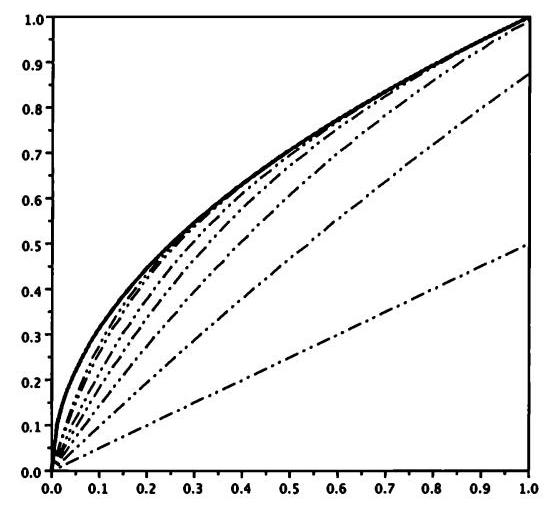
\includegraphics[width=0.4\textwidth]{images/bo_d6ik6nn7aajc739ct1l0_61_464_229_545_507_0.jpg}
\captionof{figure}{由式\eqref{eq:pn-iteration}定义的序列中的前几个多项式.}
\label{fig:pn-polynomials}
\end{figure}

\noindent 2. 对任意函数 $f \in  \mathcal{A}$ ，均有 $\left| f\right|  \in  \overline{\mathcal{A}}$ .

事实上，令 $\kappa  \doteq  \mathop{\max }\limits_{{x \in  E}}\left| {f\left( x\right) }\right|$ .可设 $\kappa  \neq  0$ .于是所有函数 ${f}_{n}\left( x\right)  = {p}_{n}\left( {{f}^{2}\left( x\right) /{\kappa }^{2}}\right)$ 均属于 $\mathcal{A}$ ，因为 $\mathcal{A}$ 是一个代数.又因 ${f}^{2}\left( x\right) /{\kappa }^{2} \in \; \left(  {0,1}\right)$ ，上一步推出收敛
\[
{f}_{n}\left( x\right)  \rightarrow  \sqrt{\frac{{f}^{2}\left( x\right) }{{\kappa }^{2}}} = \frac{\left| f\left( x\right) \right| }{\kappa },
\]

在 $x \in  E$ 上一致成立.因此 $\frac{\left| f\right| }{\kappa } \in  \overline{\mathcal{A}}$ ，从而 $\left| f\right|  \in  \overline{\mathcal{A}}$ 亦然.

\noindent 3. 现将前述论证应用于子代数 $\overline{\mathcal{A}}$ ，可得:若 $f,g \in  \overline{\mathcal{A}}$ ，则函数
\[
\max \{ f,g\}  = \frac{1}{2}\left( {f + g + \left| {f - g}\right| }\right) ,\;\min \{ f,g\}  = \frac{1}{2}\left( {f + g - \left| {f - g}\right| }\right)
\]
也属于 $\overline{\mathcal{A}}$ .

\noindent 4. 对任意两个不同点 ${y}_{1},{y}_{2} \in  E$ 及任意一对实数 ${a}_{1},{a}_{2}$ ，存在一函数 $f \in  \mathcal{A}$ ，使得 $f\left( {y}_{1}\right)  = {a}_{1}$ 且 $f\left( {y}_{2}\right)  = {a}_{2}$ .

事实上，由假设，存在一连续函数 $g \in  \mathcal{A}$ ，使得 $g\left( {y}_{1}\right)  \neq  g\left( {y}_{2}\right)$ .由于 $\mathcal{A}$ 是一个代数且包含所有常值函数，故函数
\[
f\left( x\right)  \doteq  {a}_{1} + \left( {{a}_{2} - {a}_{1}}\right) \frac{g\left( x\right)  - g\left( {y}_{1}\right) }{g\left( {y}_{2}\right)  - g\left( {y}_{1}\right) }
\]
属于 $\mathcal{A}$ ，并满足我们的要求.

\noindent 5. 对任意连续函数 $f$ 、一点 $y \in  E$ 及 $\varepsilon  > 0$ ，存在一函数 ${g}_{y} \in  \overline{\mathcal{A}}$ ，使得
\begin{equation}\tag{3.3}\label{eq:gy-ineq}
{g}_{y}\left( y\right)  = f\left( y\right) ,\;{g}_{y}\left( x\right)  \leq  f\left( x\right)  + \varepsilon ,\;\forall\,x \in  E.
\end{equation}

\begin{figure}[htbp]
    \vspace{-1 em}
\centering
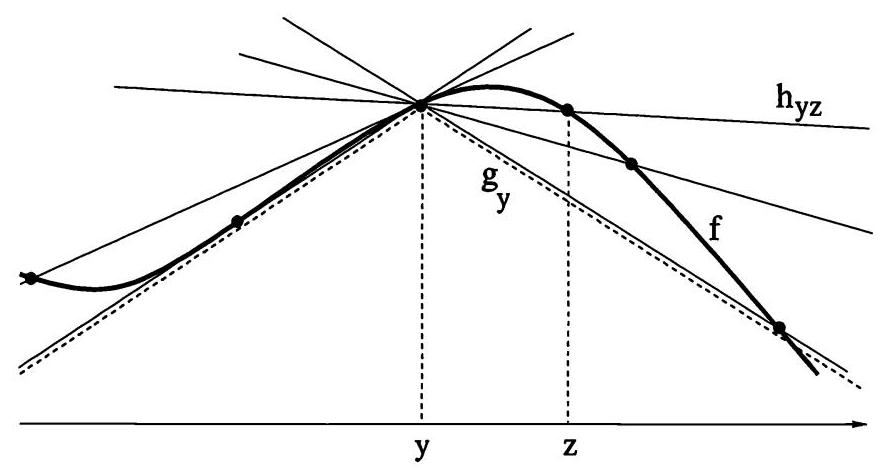
\includegraphics[width=0.7\textwidth]{images/bo_d6ik6nn7aajc739ct1l0_62_300_227_883_472_0.jpg}
\captionof{figure}{对固定 $y$ ，取有限个函数 ${h}_{yz}$ (此处绘为仿射函数)的下确界，得到一连续函数 ${g}_{y} \leq  f + \varepsilon$ ，且满足 ${g}_{y}\left( y\right)  = f\left( y\right)$ .}
\label{fig:gy-min}
\end{figure}

事实上(见图\ref{fig:gy-min})，由上一步可知，对每一点 $z \in  E$ ，存在一函数 ${h}_{yz} \in  \mathcal{A}$ ，使得 ${h}_{yz}\left( y\right)  = f\left( y\right)$ 且 ${h}_{yz}\left( z\right)  = f\left( z\right)$ .

由于 $f$ 与 ${h}_{yz}$ 均连续，故存在 $z$ 的一个开邻域 ${V}_{z}$ ，使得对每个 $x \in  {V}_{z}$ 均有 ${h}_{yz}\left( x\right)  < f\left( x\right)  + \varepsilon$ .

我们可用有限个此类邻域覆盖紧集 $E$ : $E \subseteq  {V}_{{z}_{1}} \cup  \cdots  \cup  {V}_{{z}_{m}}$ .于是函数
\[
{g}_{y}\left( x\right)  \doteq  \min \left\{  {{h}_{y{z}_{1}}\left( x\right) ,\ldots ,{h}_{y{z}_{m}}\left( x\right) }\right\}
\]

位于 $\overline{\mathcal{A}}$ 中，且满足\eqref{eq:gy-ineq}中的条件.

\begin{figure}[H]
    \vspace{-1 em}
\centering
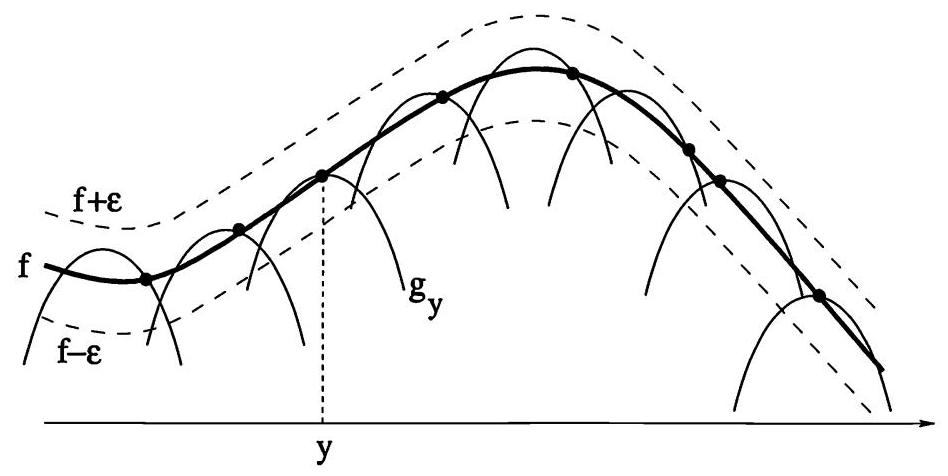
\includegraphics[width=0.7\textwidth]{images/bo_d6ik6nn7aajc739ct1l0_62_266_1404_948_476_0.jpg}
\captionof{figure}{对有限个函数 ${g}_{y}$ 取上确界，得到一个连续函数 $g$ ，使得 $f - \varepsilon  \leq  g \leq  f + \varepsilon$ .}
\label{fig:g-max}
\end{figure}

\noindent 6. $\mathcal{A}$ 的闭包是整个空间 $\mathcal{C}\left( E\right)$ .

事实上，设 $f \in  \mathcal{C}\left( E\right)$ 为任意连续函数， $\varepsilon  > 0$ 给定.对每个 $y \in  E$ ，由前一步可知存在函数 ${g}_{y} \in  \overline{\mathcal{A}}$ (见图\ref{fig:g-max})，使得
\[
{g}_{y}\left( y\right)  = f\left( y\right) ,\;{g}_{y}\left( x\right)  \leq  f\left( x\right)  + \varepsilon ,\;\forall\,x \in  E.
\]

由 $f$ 与 ${g}_{y}$ 的连续性，存在 $y$ 的一个邻域 ${U}_{y}$ ，使得
\[
{g}_{y}\left( x\right)  \geq  f\left( x\right)  - \varepsilon \;\forall\,x \in  {U}_{y}.
\]

现用有限个邻域 $E \subseteq \; {U}_{{y}_{1}} \cup  \cdots  \cup  {U}_{{y}_{\nu }}$ 覆盖紧集 $E$ .则函数
\[
g\left( x\right)  \doteq  \max \left\{  {{g}_{{y}_{1}}\left( x\right) ,\ldots ,{g}_{{y}_{\nu }}\left( x\right) }\right\}
\]

位于 $\overline{\mathcal{A}}$ 中，且满足
\[
f\left( x\right)  - \varepsilon  \leq  g\left( x\right)  \leq  f\left( x\right)  + \varepsilon \;\forall\,x \in  E.
\]

\end{proof}

满足定理\ref{thm:stone-weierstrass}全部假设的一个自然代数例子是多项式函数.

\begin{corollary}[多项式一致逼近]\label{cor:poly-approx}
设 $E$ 为 ${\mathbb{R}}^{n}$ 的紧子集， $\mathcal{A}$ 为变量 $\left( {{x}_{1},\ldots ,{x}_{n}}\right)$ 的所有实值多项式构成的族，则 $\mathcal{A}$ 在 $\mathcal{C}\left( E\right)$ 中稠密.
\end{corollary}

\begin{proof}
事实上， $\left( {{x}_{1},\ldots ,{x}_{n}}\right)$ 上的所有实值多项式构成的族是一个代数，它包含常值函数且能分离 ${\mathbb{R}}^{n}$ 中的点.因此，由定理\ref{thm:stone-weierstrass}，每个连续函数 $f : E \mapsto  \mathbb{R}$ 均可被多项式一致逼近.
\end{proof}

\subsection{复值函数}

定理\ref{thm:stone-weierstrass}证明中的一个关键要素是:若两个实值函数 $f,g$ 属于某个子代数 $\mathcal{A}$ ，则 $\max \{ f,g\}$ 与 $\min \{ f,g\}$ 也属于 $\overline{\mathcal{A}}$ .显然，此类陈述对复值函数毫无意义.事实上，Stone-Weierstrass定理在其原始形式下对复值函数并不成立.

为获得适用于函数 $f : E \mapsto  \mathbb{C}$ 的逼近结果，主要思路是将 $\mathbb{C} = \mathbb{R} \oplus  i\mathbb{R}$ 视为实数域上的二维空间.以下，对任意紧度量空间 $E$ ，我们用 ${\mathcal{C}}_{\mathbb{R}}\left( {E;\mathbb{C}}\right)$ 表示 $E$ 上所有连续复值函数构成的空间，并将其视作实数域上的向量空间.

\begin{theorem}\label{thm:stone-weierstrass-complex}
设 $E$ 为紧度量空间， $\mathcal{A}$ 为 ${\mathcal{C}}_{\mathbb{R}}\left( {E;\mathbb{C}}\right)$ 的一个子代数，它能分离点并包含常值函数；此外，若 $f \in  \mathcal{A}$ ，则其复共轭函数 $\bar{f}$ 亦属于 $\mathcal{A}$ .则 $\mathcal{A}$ 在 ${\mathcal{C}}_{\mathbb{R}}\left( {E;\mathbb{C}}\right)$ 中稠密.
\end{theorem}

\begin{proof}
1. 根据假设，若 $f \in  \mathcal{A}$ ，则其实部与虚部
\[
\operatorname{Re}\left( f\right)  = \frac{f + \bar{f}}{2},\;\operatorname{Im}\left( f\right)  = \frac{f - \bar{f}}{2}
\]
同样位于 $\mathcal{A}$ 中.设 ${\mathcal{A}}_{0}$ 为 $\mathcal{A}$ (在实数域上)的子代数，由所有取实数值的函数 $f \in  \mathcal{A}$ 构成.对 ${\mathcal{A}}_{0}$ 应用定理\ref{thm:stone-weierstrass}，可得 ${\mathcal{A}}_{0}$ 在 $\mathcal{C}\left( E\right)  = {\mathcal{C}}_{\mathbb{R}}\left( {E;\mathbb{R}}\right)$ 中稠密.

\noindent 2. 给定任意 $f \in  {\mathcal{C}}_{\mathbb{R}}\left( {E;\mathbb{C}}\right)$ ，我们将 $f$ 写为其实部与虚部之和 $f = \operatorname{Re}\left( f\right)  + i\operatorname{Im}\left( f\right)$ .由前一步可知，存在两个实值函数序列 ${g}_{n},{h}_{n} \in  {\mathcal{A}}_{0}$ ，使得
\begin{equation}\tag{3.4}\label{eq:gh-conv}
{g}_{n} \rightarrow  \operatorname{Re}\left( f\right) ,\;{h}_{n} \rightarrow  \operatorname{Im}\left( f\right)
\end{equation}

作为 $n \rightarrow  \infty$ ，在 $E$ 上一致地.

考虑序列 ${f}_{n} \doteq  {g}_{n} + i{h}_{n} \in  {\mathcal{A}}_{0} + i{\mathcal{A}}_{0} = \mathcal{A}$ .由\eqref{eq:gh-conv}式，我们有一致收敛性 ${f}_{n} \rightarrow  f$.因此 $\overline{\mathcal{A}} = {\mathcal{C}}_{\mathbb{R}}\left( {E;\mathbb{C}}\right)$ .
\end{proof}

\begin{instance}[复三角多项式]\label{ins:complex-trig-poly}
设 $E$ 为 ${\mathbb{R}}^{2}$ 中的单位圆周 $\left\{  {{x}^{2} + {y}^{2} = 1}\right\}$ . $E$ 上的点将由角度 $\theta  \in  \left(  {0,{2\pi }}\right)$ 参数化.令 $\mathcal{A}$ 为所有复三角多项式构成的代数:
\begin{equation}\tag{3.5}\label{eq:complex-trig}
p\left( \theta \right)  = \mathop{\sum }\limits_{{n =  - N}}^{N}{\mathrm{c}}_{n}{e}^{in\theta }
\end{equation}

其中 $N \geq  0$ 为任意整数，系数 ${\mathrm{c}}_{n}$ 为复数.显然， $\mathcal{A}$ 是一个代数，包含常值函数，且能分离点.此外， $p \in  \mathcal{A}$ 也蕴含 $\bar{p} \in  \mathcal{A}$ .由定理\ref{thm:stone-weierstrass-complex} 可知，所有这类复三角多项式构成的族在 ${\mathcal{C}}_{\mathbb{R}}\left( {E;\mathbb{C}}\right)$ 中稠密.
\end{instance}

沿用例\ref{ins:complex-trig-poly}，我们现在证明:一个实值的连续周期函数可用如下形式的三角多项式一致逼近
\begin{equation}\tag{3.6}\label{eq:real-trig}
q\left( x\right)  = \mathop{\sum }\limits_{{k = 0}}^{N}{\alpha }_{k}\cos {kx} + \mathop{\sum }\limits_{{k = 1}}^{N}{\beta }_{k}\sin {kx}.
\end{equation}

此处 $N \geq  1$ 为任意整数，而 ${\alpha }_{n},{\beta }_{n}$ 为实数.

\begin{corollary}[三角多项式对周期函数的逼近]\label{cor:trig-approx-periodic}
设 $f : \mathbb{R} \mapsto  \mathbb{R}$ 是一个连续函数，且以 ${2\pi }$ 为周期.则对任意 $\varepsilon  > 0$ ，存在形如 \eqref{eq:real-trig} 的三角多项式 $q$ ，使得
\begin{equation}\tag{3.7}\label{eq:trig-approx-bound}
\left| {q\left( x\right)  - f\left( x\right) }\right|  \leq  \varepsilon ,\;\forall\,x \in  \mathbb{R}.
\end{equation}
\end{corollary}

\begin{proof}
由假设，对每个 $x \in  \mathbb{R}$ ，均有 $f\left( {x + {2\pi }}\right)  = f\left( x\right)$ .如例\ref{ins:complex-trig-poly}所示，存在一个形如\eqref{eq:complex-trig}的复三角多项式 $p$ ，使得
\begin{equation}\tag{3.8}\label{eq:complex-approx-bound}
\left| {p\left( x\right)  - f\left( x\right) }\right|  \leq  \varepsilon \;\forall\,x \in  \mathbb{R}.
\end{equation}

考虑复系数 ${c}_{n} = {a}_{n} + i{b}_{n}$ ，其中 ${a}_{n},{b}_{n} \in  \mathbb{R}$ .记 $q\left( x\right)  \doteq  \operatorname{Re}p\left( x\right)$ 为 $p$ 的实部，我们计算
\[
q\left( x\right)  = \mathop{\sum }\limits_{{n =  - N}}^{N}{a}_{n}\cos {nx} - \mathop{\sum }\limits_{{n =  - N}}^{N}{b}_{n}\sin {nx} = \mathop{\sum }\limits_{{n = 0}}^{N}{\alpha }_{n}\cos {nx} + \mathop{\sum }\limits_{{n = 1}}^{N}{\beta }_{n}\sin {nx},
\]

其中${\alpha }_{0} = {a}_{0},\;{\alpha }_{n} = {a}_{-n} + {a}_{n},\;{\beta }_{n} = {b}_{-n} - {b}_{n}\,\text{若}\,n \geq  1.$

由于 $f$ 是实值函数，由\eqref{eq:complex-approx-bound}式可得
{\setjot[-2]\begin{align*}
\left| {q\left( x\right)  - f\left( x\right) }\right|  &= \left| {\operatorname{Re}p\left( x\right)  - \operatorname{Re}f\left( x\right) }\right| \\
&\leq  \left| {p\left( x\right)  - f\left( x\right) }\right|  \leq  \varepsilon \;,\forall\,x \in  \mathbb{R}.\qedhere
\end{align*}}
\end{proof}

\begin{remark}\label{rem:even-odd-trig}
若周期函数 $f$ 是偶函数，即满足 $f\left( x\right)  = f\left( {-x}\right)$ ，则它可用形如\eqref{eq:real-trig}的三角多项式逼近，且对每个 $k \geq  1$ 均有 ${\beta }_{k} = 0$ ，即仅含有限个余弦函数的和.

若 $f$ 是奇函数，即满足 $f\left( x\right)  =  - f\left( {-x}\right)$ ，则在\eqref{eq:real-trig}式中可取对每个 $k \geq  0$ 均有 ${\alpha }_{k} = 0$ .换言之， $f$ 可由有限个正弦函数的和逼近.
\end{remark}

\section{Ascoli紧性定理}

在有限维空间中，根据波尔查诺-Weierstrass定理，每个有界序列都存在收敛子列.另一方面，如第 2 章定理 2.22 所示，该紧性性质在任意无限维赋范空间中均不成立.例如，在空间 $\mathcal{C}\left( \left(  {0,1}\right)  \right)$ 中，连续函数序列 ${f}_{n}\left( x\right)  = {x}^{n}$ 或 ${f}_{n}\left( x\right)  = \sin {nx}$ 虽有界，却不含一致收敛子列.因此自然提出问题:函数族 ${f}_{n}$ 需具备何种附加性质，才能保证存在一致收敛子列？Ascoli定理借助等度连续概念给出了一个回答.
\begin{definition}[等度连续]
    设 $E$ 为一度量空间.一族连续函数 $\mathcal{F} \subset  \mathcal{C}\left( E\right)$ 称为\colorbf{等度连续的}，若对任意 $x \in  E$ 和 $\varepsilon  > 0$ ，存在 $\delta  > 0$ ，使得对所有函数 $f \in  \mathcal{F}$，都有
\begin{equation}\tag{3.9}\label{eq:equicontinuity-point}
d\left( {y,x}\right)  < \delta \implies \left| {f\left( y\right)  - f\left( x\right) }\right|  < \varepsilon
\end{equation}
\end{definition}
注意此处 $\delta  > 0$ 可依赖于 $x$ 和 $\varepsilon$ ，但不依赖于特定函数 $f \in  \mathcal{F}$ .

\begin{lemma}\label{lem:equicontinuous-uniform}
设 $E$ 为紧致度量空间， $\mathcal{F} \subset  \mathcal{C}\left( E\right)$ 为等度连续族，则 $\mathcal{F}$ 是一致等度连续的.即对任意 $\varepsilon  > 0$ ，存在 $\delta  > 0$ ，使得
\begin{equation}\tag{3.10}\label{eq:equicontinuity-uniform}
d\left( {x,y}\right)  < \delta \implies \left| {f\left( x\right)  - f\left( y\right) }\right|  < \varepsilon ,\;\forall\,x,y \in  E,\;f \in  \mathcal{F}.
\end{equation}
\end{lemma}

\begin{proof}
给定 $\varepsilon  > 0$ .对每个 $x \in  E$ ，选取 $\delta  = \delta \left( x\right)  > 0$ ，使得\eqref{eq:equicontinuity-point}式对所有函数 $f \in  \mathcal{F}$ 同时成立.由紧性，可用有限个球覆盖空间 $E$ :
\[
E \subseteq  B\left( {{x}_{1},{\delta }_{1}}\right)  \cup  \cdots  \cup  B\left( {{x}_{n},{\delta }_{n}}\right) ,
\]
其中 ${\delta }_{i} = \delta \left( {x}_{i}\right)$ .选取足够小的 $\rho  > 0$ ，使得对每个 $x \in  E$ ，球 $B\left( {x,\rho }\right)$ 完全包含于某个球 $B\left( {{x}_{i},{\delta }_{i}}\right)$ 内.

现在假设 $d\left( {x,y}\right)  < \rho$ .则存在$k \in  \{ 1,\ldots ,n\}$ ，使得 $x,y \in  B\left( {{x}_{k},{\delta }_{k}}\right)$ .这意味着
\[
\left| {f\left( x\right)  - f\left( y\right) }\right|  \leq  \left| {f\left( x\right)  - f\left( {x}_{k}\right) }\right|  + \left| {f\left( y\right)  - f\left( {x}_{k}\right) }\right|  \leq  \varepsilon  + \varepsilon
\]
对每个函数 $f \in  \mathcal{F}$ 均成立.由于 $\varepsilon  > 0$ 是任意的，故该引理得证.
\end{proof}

若 $E$ 是紧度量空间，则 $\mathcal{C}\left( E\right)  = \mathcal{B}C\left( E\right)$ 是Banach空间.由完备性可知，对子集 $\mathcal{F} \subset  \mathcal{C}\left( E\right)$ ，以下性质等价:

(i) $\mathcal{F}$ 是相对紧的，即闭包 $\overline{\mathcal{F}}$ 是紧集.

(ii) $\mathcal{F}$ 是预紧的，即对任意 $\varepsilon  > 0$ ，它可被有限个半径为 $\varepsilon$ 的球覆盖.

(iii) 对任意连续函数序列 ${f}_{k} \in  \mathcal{F}$ ，均可提取一个子列，该子列在 $E$ 上一致收敛于某个函数 $f$ .

\begin{theorem}[Ascoli 定理]\label{thm:ascoli}
设 $E$ 是一个紧度量空间， $\mathcal{F} \subset  \mathcal{C}\left( E\right)$ 是一族等度连续函数，且满足
\begin{equation}\tag{3.11}\label{eq:ascoli-pointwise-bounded}
    \sup_{{f \in  \mathcal{F}}}\left| {f\left( x\right) }\right|  < \infty, \;\forall\,x \in  E.
\end{equation}

则 $\mathcal{F}$ 是 $\mathcal{C}\left( E\right)$ 中的相对紧子集.
\end{theorem}

\begin{proof}
只需证 $\mathcal{F}$ 是预紧的.

\noindent 1. 给定 $\varepsilon  > 0$ .由引理\ref{lem:equicontinuous-uniform}，存在 $\delta  > 0$ 使得\eqref{eq:equicontinuity-uniform}成立.由于 $E$ 是紧集，它可被有限个半径为$\delta$ 的球覆盖，记为
\[
E \subseteq  \mathop{\bigcup }\limits_{{i = 1}}^{n}B\left( {{x}_{i},\delta }\right) .
\]

由假设\eqref{eq:ascoli-pointwise-bounded}，
\[
M \doteq  \mathop{\max }\limits_{{i \in  \{ 1,\ldots ,n\} }}\mathop{\sup }\limits_{{f \in  \mathcal{F}}}\left| {f\left( {x}_{i}\right) }\right|  < \infty .
\]

现选取有限个数 ${\alpha }_{1},\ldots ,{\alpha }_{m}$ ，使得球 $B\left( {{\alpha }_{j},\varepsilon }\right)$ 覆盖紧区间 $\left(  {-M,M}\right)$ .

\noindent 2. 考虑所有映射 $\theta  : \left\{  {{x}_{1},\ldots ,{x}_{n}}\right\}   \mapsto  \left\{  {{\alpha }_{1},\ldots ,{\alpha }_{m}}\right\}$ 构成的集合 $\Theta$ .这是一个有限集；事实上，恰有 ${m}^{n}$ 个这样的映射.对每个 $\theta  \in  \Theta$ ，定义连续函数族
\[
{\mathcal{F}}_{\theta } \doteq  \left\{  {f \in  \mathcal{F};f\left( {x}_{i}\right)  \in  B\left( {\theta \left( {x}_{i}\right) ,\varepsilon }\right) \forall\,i = 1,\ldots ,n}\right\}  .
\]

由于区间 $\left(  {-M,M}\right)$ 被球 $B\left( {{\alpha }_{j},\varepsilon }\right)$ 覆盖，显然有 $\mathop{\bigcup }\limits_{{\theta  \in  \Theta }}{\mathcal{F}}_{\theta } = \mathcal{F}$

\noindent 3. 我们声称每个集合 ${\mathcal{F}}_{\theta }$ 的直径为 $\leq  {4\varepsilon }$ .事实上，设 $f,g \in  {\mathcal{F}}_{\theta }$ .对任意 $x \in  E$ ，选取指标 $i$ 使得 $x \in  B\left( {{x}_{i},\delta }\right)$ .于是有
{\setjot[-2]\begin{align*}
    &\left| {f\left( x\right)  - g\left( x\right) }\right|   \\
    &\leq  \left| {f\left( x\right)  - f\left( {x}_{i}\right) }\right|  + \left| {f\left( {x}_{i}\right)  - \theta \left( {x}_{i}\right) }\right|  + \left| {\theta \left( {x}_{i}\right)  - g\left( {x}_{i}\right) }\right|  + \left| {g\left( {x}_{i}\right)  - g\left( x\right) }\right| \\
    &\leq  \varepsilon  + \varepsilon  + \varepsilon  + \varepsilon .
\end{align*}}

因此
\[
\| f - g{\| }_{\mathcal{C}} \doteq  \mathop{\max }\limits_{{x \in  E}}\left| {f\left( x\right)  - g\left( x\right) }\right|  \leq  {4\varepsilon }.
\]

上述论证表明:对任意 $\varepsilon  > 0$ ，集合 $\mathcal{F}$ 均可被有限个直径为 $\leq  {4\varepsilon }$ 的集合覆盖，故也可被有限个半径为 ${4\varepsilon }$ 的闭球覆盖.由于 $\varepsilon$ 是任意的，这证明了 $\mathcal{F}$ 是预紧的.
\end{proof}

上述定理可轻易推广至取值于复平面 $\mathbb{C}$ 或欧氏空间 ${\mathbb{R}}^{n}$ 的函数.

\begin{corollary}\label{cor:ascoli-rn-subsequence}
设 $E$ 为一紧致度量空间， ${\left( {f}_{k}\right) }_{k \geq  1}$ 为一列从 $E$ 到 ${\mathbb{R}}^{n}$ 的连续函数，且满足

(i) 函数族 $\left\{  {f}_{k}\right\}$ 等度连续；

(ii) 对每个 $x \in  E$ ， $\mathop{\sup }\limits_{{k \geq  1}}\left| {{f}_{k}\left( x\right) }\right|  < \infty$ 成立.

则序列 ${\left( {f}_{k}\right) }_{k \geq  1}$ 存在一致收敛的子列.
\end{corollary}

\begin{proof}
我们写出各分量:
\[
{f}_{k}\left( x\right)  = \left( {{f}_{k,1}\left( x\right) ,{f}_{k,2}\left( x\right) ,\ldots ,{f}_{k,n}\left( x\right) }\right)  \in  {\mathbb{R}}^{n}.
\]

对纯量函数列 ${\left( {f}_{k,1}\right) }_{k \geq  1}$ 应用定理\ref{thm:ascoli}，可提取一子列，使这些第一分量在 $E$ 上一致收敛；再从此子列中提取进一步的子列，使第二分量一致收敛，依此类推.经过 $n$ 步后，得到一子列，其所有分量均在 $E$ 上一致收敛.
\end{proof}

\section{Hölder 连续函数}
\begin{definition}[Hölder 连续函数]\label{def:holder-continuous}
    设 $\Omega  \subset  {\mathbb{R}}^{n}$ 为一开集， $0 < \gamma  \leq  1$ .若存在常数 $C$ ，使得对函数 $f : \Omega  \mapsto  \mathbb{R}$ 有
\[
\left| {f\left( x\right)  - f\left( y\right) }\right|  \leq  C{\left| x - y\right| }^{\gamma }\;\forall\,x,y \in  \Omega .
\]
则称 $f : \Omega  \mapsto  \mathbb{R}$ 为指数为 $\gamma$ 的\colorbf{Hölder 连续函数}.
\end{definition}
\begin{definition}[Hölder 连续函数空间]\label{def:holder-function-space}
    记 ${\mathcal{C}}^{0,\gamma }\left( \Omega \right)$ 为 $\Omega$ 上所有有界 Hölder 连续函数构成的空间，其范数为
\begin{equation}\tag{3.12}\label{eq:holder-norm-0-gamma}
\| f{\| }_{{\mathcal{C}}^{0,\gamma }\left( \Omega \right) } \doteq  \mathop{\sup }\limits_{{x \in  \Omega }}\left| {f\left( x\right) }\right|  + \mathop{\sup }\limits_{{x,y \in  \Omega ,x \neq  y}}\frac{\left| f\left( x\right)  - f\left( y\right) \right| }{{\left| x - y\right| }^{\gamma }}.
\end{equation}
\end{definition}


更一般地，给定整数 $k \geq  0$ ，记 ${\mathcal{C}}^{k,\gamma }\left( \Omega \right)$ 为所有直至 $k$ 阶偏导数均为 Hölder 连续的连续函数构成的空间.该空间赋予范数.

\begin{definition}[$\mathcal{C}^{k,\gamma}$空间的范数]
    $\mathcal{C}^{k,\gamma}$是所有直至 $k$ 阶偏导数均为 Hölder 连续的连续函数构成的空间，其范数定义为
    \begin{equation}\tag{3.13}\label{eq:holder-norm-k-gamma}
\| f{\| }_{{\mathcal{C}}^{k,\gamma }\left( \Omega \right) } \doteq  \mathop{\sum }\limits_{{\left| \alpha \right|  \leq  k}}\left( {\mathop{\sup }\limits_{{x \in  \Omega }}\left| {{D}^{\alpha }f\left( x\right) }\right| }\right)  + \mathop{\sum }\limits_{{\left| \alpha \right|  = k}}\left( {\mathop{\sup }\limits_{{x,y \in  \Omega ,x \neq  y}}\frac{\left| {D}^{\alpha }f\left( x\right)  - {D}^{\alpha }f\left( y\right) \right| }{{\left| x - y\right| }^{\gamma }}}\right)\footnotemark.
\end{equation}
\end{definition}

\footnotetext{给定一多重指标 $\alpha  = \left( {{\alpha }_{1},\ldots ,{\alpha }_{n}}\right)$ ，我们用记号 ${D}^{\alpha }f = {\left( \frac{\partial }{{\partial }_{{x}_{1}}}\right) }^{{\alpha }_{1}}\cdots {\left( \frac{\partial }{{\partial }_{{x}_{n}}}\right) }^{{\alpha }_{n}}f$ 表示 $f$ 的 $\left| \alpha \right|  = {\alpha }_{1} + \cdots  + {\alpha }_{n}$ 阶偏导数.}


\begin{theorem}[Hölder 空间完备性]\label{thm:holder-banach}
设 $\Omega  \subseteq  {\mathbb{R}}^{n}$ 为一开集.对任意整数 $k \geq  0$ 及任意 $0 < \gamma  \leq  1$ ，空间 ${\mathcal{C}}^{k,\gamma }\left( \Omega \right)$ 是 Banach 空间.
\end{theorem}

\begin{proof}
\eqref{eq:holder-norm-k-gamma}定义一范数是显然的.为证空间 ${\mathcal{C}}^{k,\gamma }\left( \Omega \right)$ 完备，设 ${\left( {f}_{m}\right) }_{m \geq  1}$ 是关于范数\eqref{eq:holder-norm-k-gamma}的 Cauchy 列.则对每个 $x \in  \Omega$ ，序列 ${f}_{m}\left( x\right)$ 是 Cauchy 列，且在 $\Omega$ 上一致收敛于某值 $f\left( x\right)$ .

该假设还蕴含:对每个 $\left| \alpha \right|  \leq  k$ ，偏导数列 ${D}^{\alpha }{f}_{m}$ 是 Cauchy 列；故其在 $\Omega$ 上一致收敛于某连续函数 ${v}_{\alpha }\left( x\right)  = {D}^{\alpha }f\left( x\right)$ .

还需证明收敛 ${f}_{m} \rightarrow  f$ 在 ${\mathcal{C}}^{k,\gamma }\left( \Omega \right)$ 范数下也成立.换言之，对 $\left| \alpha \right|  = k$ ，需证明
\begin{equation}\tag{3.14}\label{eq:holder-seminorm-conv}
\mathop{\lim }\limits_{{m \rightarrow  \infty }}\mathop{\sup }\limits_{{x,y \in  \Omega ,x \neq  y}}\frac{\left| {D}^{\alpha }\left( {f}_{m} - f\right) \left( x\right)  - {D}^{\alpha }\left( {f}_{m} - f\right) \left( y\right) \right| }{{\left| x - y\right| }^{\gamma }} = 0.
\end{equation}

由假设知，
\[
\mathop{\lim }\limits_{{m,n \rightarrow  \infty }}\mathop{\sup }\limits_{{x,y \in  \Omega ,x \neq  y}}\frac{\left| {D}^{\alpha }\left( {f}_{m} - {f}_{n}\right) \left( x\right)  - {D}^{\alpha }\left( {f}_{m} - {f}_{n}\right) \left( y\right) \right| }{{\left| x - y\right| }^{\gamma }} = 0.
\]

因此，对任意 $\varepsilon  > 0$ ，存在足够大的 $N$ ，使得
\[
\mathop{\sup }\limits_{{x,y \in  \Omega ,x \neq  y}}\frac{\left| {D}^{\alpha }\left( {f}_{m} - {f}_{n}\right) \left( x\right)  - {D}^{\alpha }\left( {f}_{m} - {f}_{n}\right) \left( y\right) \right| }{{\left| x - y\right| }^{\gamma }} \leq  \varepsilon \forall\,m,n \geq  N.
\]

固定 $m$ 并令 $n \rightarrow  \infty$ ，可得
\[
\mathop{\sup }\limits_{{x,y \in  \Omega ,x \neq  y}}\frac{\left| {D}^{\alpha }\left( {f}_{m} - f\right) \left( x\right)  - {D}^{\alpha }\left( {f}_{m} - f\right) \left( y\right) \right| }{{\left| x - y\right| }^{\gamma }} \leq  \varepsilon \forall\,m \geq  N.
\]

由于 $\varepsilon  > 0$ 是任意的，故\eqref{eq:holder-seminorm-conv}得证.
\end{proof}

\section{习题}

\begin{rbhw}[index=1]
设 $E$ 为紧致度量空间.假设一族实值连续函数 $\mathcal{F} \subset  \mathcal{C}\left( E\right)$ 满足以下两个条件:
\begin{enumerate}[(i)]
\item 对每个 $x,y \in  E$ 和 $a,b \in  \mathbb{R}$ ，存在函数 $f \in  \mathcal{F}$ ，使得 $f\left( x\right)  = a$ 且 $f\left( y\right)  = b$.
\item 若 $f,g \in  \mathcal{F}$ ，则函数 $\max \{ f,g\}$ 与 $\min \{ f,g\}$ 均属于该闭包.
\end{enumerate}
证明 $\mathcal{F}$ 在 $\mathcal{C}\left( E\right)$ 中稠密.
\end{rbhw}

\begin{rbhw}
判定下列命题的真假(证明或举反例).
\begin{enumerate}[(i)]
\item 对任意连续函数 $f : \mathbb{R} \mapsto  \mathbb{R}$ (可能无界)，存在一列多项式 ${\left( {p}_{n}\right) }_{n \geq  1}$ ，使得 ${p}_{n}\left( x\right)  \rightarrow  f\left( x\right)$ 在每个有界区间 $\left(  {a,b}\right)$ 上一致成立.(注:此处多项式序列应与区间 $\left(  {a,b}\right)$ 无关.)
\item 存在一列多项式 ${p}_{n}$ ，在 $\mathbb{R}$ 上一致收敛于函数 $f\left( x\right)  = {e}^{-{x}^{2}}$ .
\end{enumerate}
\end{rbhw}

\begin{rbhw}
设 $g : \left(  {0,\pi }\right)   \mapsto  \mathbb{R}$ 为连续函数.
\begin{enumerate}[(i)]
\item 证明:对任意 $\varepsilon  > 0$ ，存在形如
\[
p\left( x\right)  = \mathop{\sum }\limits_{{k = 0}}^{N}{b}_{k}\cos {kx}
\]
的三角多项式，使得对每个 $x \in  \left(  {0,\pi }\right)$ 均有 $\left| {p\left( x\right)  - g\left( x\right) }\right|  < \varepsilon$ .
\item 若 $g\left( 0\right)  = g\left( \pi \right)  = 0$ ，证明:对任意 $\varepsilon  > 0$ ，存在形如
\[
p\left( x\right)  = \mathop{\sum }\limits_{{k = 1}}^{N}{a}_{k}\sin {kx}
\]
使得对每个 $x \in  \left(  {0,\pi }\right)$ ，均有 $\left| {p\left( x\right)  - g\left( x\right) }\right|  < \varepsilon$ .
\end{enumerate}
\end{rbhw}

\begin{rbhw}
设 $f : \mathbb{R} \mapsto  \mathbb{R}$ 连续可微.证明:对任意有界区间 $\left(  {a,b}\right)$ ，存在一多项式序列 ${p}_{n}$ ，使得 ${p}_{n} \rightarrow  f$ 且 ${p}_{n}^{\prime } \rightarrow  {f}^{\prime }$ 在 $\left(  {a,b}\right)$ 上一致成立.
\end{rbhw}

\begin{rbhw}
设 $E$ 为 ${\mathbb{R}}^{2}$ 中的单位圆 $\left\{  {{x}^{2} + {y}^{2} = 1}\right\}$ . $E$ 上的点以角度 $\theta  \in  \left(  {0,{2\pi }}\right)$ 参数化.令 $\mathcal{A}$ 为所有形如下式的复三角多项式构成的族
\[
p\left( \theta \right)  = \mathop{\sum }\limits_{{n = 0}}^{N}{\mathrm{c}}_{n}{e}^{in\theta }
\]
其中 $N \geq  0$ 为任意整数， ${\mathrm{c}}_{n}$ 为复值系数.
\begin{enumerate}[(i)]
\item $\mathcal{A}$ 是否构成一个代数？
\item $\mathcal{A}$ 是否包含常值函数并能分离点？
\item $\mathcal{A}$ 在所有连续复值函数 $f$ : $E \mapsto  \mathbb{C}$ 构成的空间上是否稠密？
\end{enumerate}
\end{rbhw}

\begin{rbhw}
设 $\Omega  \subset  {\mathbb{R}}^{n}$ 为有界开集.证明: $n$ 元多项式族 $p = p\left( {{x}_{1},{x}_{2},\ldots ,{x}_{n}}\right)$ 在空间 ${\bm{L}}^{p}\left( \Omega \right)$ 中稠密，对每个 $1 \leq  p < \infty$ 均成立.
\end{rbhw}

\begin{rbhw}
考虑矩形 $Q = \{ \left( {x,y}\right) ;x \in  \left(  {0,a}\right)  ,y \in  \left(  {0,b}\right)  \}$ .
\begin{enumerate}[(i)]
\item 对任意定义在 $Q$ 上的连续函数 $f = f\left( {x,y}\right)$ 及任意 $\varepsilon  > 0$ ，构造有限个连续函数 ${g}_{1},\ldots ,{g}_{N} : \left(  {0,a}\right)   \mapsto  \mathbb{R}$ 与 ${h}_{1},\ldots ,{h}_{n} : \left(  {0,b}\right)   \mapsto  \mathbb{R}$ ，使得
\[
\left| {f\left( {x,y}\right)  - \mathop{\sum }\limits_{{i = 1}}^{N}{g}_{i}\left( x\right) {h}_{i}\left( y\right) }\right|  \leq  \varepsilon \forall\,\left( {x,y}\right)  \in  Q.
\]
\item 对任意在 $Q$ 边界上消失的连续函数 $f : Q \mapsto  \mathbb{R}$ ，证明可选取整数 $M \geq  1$ 及有限个系数 ${\mathrm{c}}_{mn},1 \leq  m,n \leq  M$ ，使得
\[
\left| {f\left( {x,y}\right)  - \mathop{\sum }\limits_{{m,n = 1}}^{M}{\mathrm{c}}_{mn}\sin \frac{\pi mx}{a}\sin \frac{\pi ny}{b}}\right|  \leq  \varepsilon \forall\,\left( {x,y}\right)  \in  Q.
\]
\end{enumerate}
\end{rbhw}

\begin{rbhw}
设 $\Omega  \subset  {\mathbb{R}}^{n}$ 为有界开集，且 $0 < \gamma  \leq  1$ .证明嵌入 ${\mathcal{C}}^{0,\gamma }\left( \Omega \right)  \subset   \subset  {\mathcal{C}}^{0}\left( \Omega \right)$ 是紧的.即:若 ${\left( {f}_{n}\right) }_{n \geq  1}$ 是 ${\mathcal{C}}^{0,\gamma }\left( \Omega \right)$ 中的有界序列，则它必存在一个在 ${\mathcal{C}}^{0}\left( \Omega \right)$ 中收敛的子列.
\end{rbhw}

\begin{rbhw}
确定使以下函数属于Hölder空间 ${\mathcal{C}}^{0,\gamma }\left( {( 0,1) }\right)$ 的 $0 < \gamma  \leq  1$ 的取值.
\[
{f}_{1}\left( x\right)  = {x}^{1/3},\;{f}_{2}\left( x\right)  = \sqrt{x} \cdot  \sin \frac{1}{x},\;{f}_{3}\left( x\right)  = x\left| {\ln x}\right| .
\]
\end{rbhw}

\begin{rbhw}
解释以下论证错在何处.
\begin{quote}
设 $0 < \gamma  \leq  1$ ，并设 ${\left( {f}_{n}\right) }_{n \geq  1}$ 为Hölder空间 ${\mathcal{C}}^{0,\gamma }\left( \left(  {0,1}\right)  \right)$ 中的一列函数，且对每个 $n$ 均有 ${\norm{f}_{n}}_{{\mathcal{C}}^{0,\gamma }} \leq  1$ .由于函数列 ${f}_{n}$ 一致有界且等度连续，由Ascoli定理可知，可提取一子列，其在 $x \in  \left(  {0,1}\right)$ 上一致收敛于某个极限函数 $f$ .现易验证 $\| f{\| }_{{\mathcal{C}}^{0,\gamma }} \leq  1$ .这表明 ${\mathcal{C}}^{0,\gamma }$ 中的闭单位球是紧的，从而由第2章定理2.22可知，空间 ${\mathcal{C}}^{0,\gamma }$ 是有限维的.
\end{quote}
\end{rbhw}

\begin{rbhw}
设 $\varphi  : {\mathbb{R}}_{ + } \mapsto  {\mathbb{R}}_{ + }$ 为一光滑函数，满足
\[
\varphi \left( 0\right)  = 0,\;{\varphi }^{\prime }\left( s\right)  > 0,\;{\varphi }^{\prime \prime }\left( s\right)  \leq  0\;\forall\,s > 0.
\]
给定开集 $\Omega  \subseteq  {\mathbb{R}}^{n}$ ，考虑连续函数空间
\[
{\mathcal{C}}^{\varphi }\left( \Omega \right)  \doteq  \left\{  {f : \Omega  \mapsto  \mathbb{R};\| f{\| }_{\varphi } \doteq  \mathop{\sup }\limits_{x}\left| {f\left( x\right) }\right|  + \mathop{\sup }\limits_{{x \neq  y}}\frac{\left| f\left( x\right)  - f\left( y\right) \right| }{\varphi \left( \left| {x - y}\right| \right) } < \infty }\right\}  .
\]
证明 ${\mathcal{C}}^{\varphi }\left( \Omega \right)$ 是一个Banach空间.(注:此处函数 $\varphi$ 可视为一个连续模；当 $\varphi \left( s\right)  = {s}^{\gamma }$ 且 $0 < \gamma  \leq  1$ 时，有 $\left. {{\mathcal{C}}^{\varphi }\left( \Omega \right)  = {\mathcal{C}}^{0,\gamma }\left( \Omega \right) \text{ . }}\right)$
\end{rbhw}

\begin{rbhw}
证明Ascoli定理如下更一般的形式:设 $E$ 为一紧度量空间， $K$ 为赋范空间 $X$ 的紧子集.假设映射列 ${\phi }_{n} : E \mapsto  K$ 是等度连续的，即:对任意 $x \in  E$ 与 $\varepsilon  > 0$ ，存在 $\delta  > 0$ 使得
\[
d\left( {y,x}\right)  < \delta \implies\norm{{\phi }_{n}\left( y\right)  - {\phi }_{n}\left( x\right) } < \varepsilon \forall\,n \geq  1.
\]
则序列 ${\left( {\phi }_{n}\right) }_{n \geq  1}$ 存在一致收敛的子列.
\end{rbhw}

\chapter{有界线性算子}
\vspace{-2em}

本章将更详细地考察Banach空间中的线性算子.如第2章一样， $\mathcal{B}\left( {X,Y}\right)$ 表示所有有界线性算子 $\Lambda  : X \mapsto  Y$ 构成的空间，其范数为
\[
\| \Lambda \|  \doteq  \mathop{\sup }\limits_{{\| x\|  \leq  1}}\| {\Lambda x}\| .
\]

我们首先给出一些基于Baire纲定理的结果.

\section{一致有界性原理}

\begin{theorem}[Banach-Steinhaus一致有界性原理]\label{thm:banach-steinhaus}
设 $X,Y$ 为Banach空间， $\mathcal{F} \subset  \mathcal{B}\left( {X,Y}\right)$ 为一族有界线性算子.则要么 $\mathcal{F}$ 是一致有界的，即
\[
\mathop{\sup }\limits_{{\Lambda  \in  \mathcal{F}}}\| \Lambda \|  < \infty ,
\]
要么存在一个稠密集 $S \subset  X$ ，使得
\begin{equation}\tag{4.1}\label{eq:unif-bddness-blowup}
\mathop{\sup }\limits_{{\Lambda  \in  \mathcal{F}}}\| {\Lambda x}\|  = \infty ,\;\forall\,x \in  S.
\end{equation}
\end{theorem}

\begin{proof}
对每个整数 $n$ ，考虑开集
\begin{equation}\tag{4.2}\label{eq:Sn-def}
{S}_{n} \doteq  \{ x \in  X;\exists\,\Lambda\in\mathcal{F},\| {\Lambda x}\|  > n\} .
\end{equation}

若这些集合中有一个(比如 ${S}_{k}$ )在 $X$ 中不稠密，则存在 ${x}_{0} \in  X$ 和半径 $r > 0$ ，使得闭球 $\bar{B}\left( {{x}_{0},r}\right)$ 与 ${S}_{k}$ 不相交.换言之，
\[
\| {\Lambda x}\|  \leq  k\forall\,\Lambda  \in  \mathcal{F},\;x \in  \bar{B}\left( {{x}_{0},r}\right) .
\]

若此时 $\| x\|  \leq  r$ ，则
\[
\| {\Lambda x}\|  = \norm{\Lambda \left( {{x}_{0} + x}\right)  - \Lambda {x}_{0}} \leq  \norm{\Lambda \left( {{x}_{0} + x}\right) } + \norm{\Lambda {x}_{0}} \leq  {2k}
\]
对所有 $\Lambda  \in  \mathcal{F}$ 成立.因此
\[
\| \Lambda \|  \doteq  \mathop{\sup }\limits_{{\| x\|  \leq  1}}\| {\Lambda x}\|  = \frac{1}{r}\mathop{\sup }\limits_{{\| x\|  \leq  r}}\| {\Lambda x}\|  \leq  \frac{2k}{r}
\]
对每个 $\Lambda  \in  \mathcal{F}$ 成立.此时，算子族 $\mathcal{F}$ 一致有界.

另一种可能是:式\eqref{eq:Sn-def}中的开集 ${S}_{n}$ 全都在 $X$ 中稠密.由Baire纲定理，交集 $S \doteq  \mathop{\bigcap }\limits_{{n \geq  1}}{S}_{n}$ 在 $X$ 中稠密.由构造可知，对每个 $x \in  S$ 和 $n \geq  1$ ，均存在算子 $\Lambda  \in  \mathcal{F}$ ，使得 $\| {\Lambda x}\|  > n$ 成立.故\eqref{eq:unif-bddness-blowup}成立.
\end{proof}

\begin{remark}\label{rem:uniform-boundedness-pointwise}
由定理\ref{thm:banach-steinhaus}可知，若算子族 $\Lambda  \in  \mathcal{B}\left( {X,Y}\right)$ 在单位球上逐点有界，则其一致有界.换言之，条件
\[
\mathop{\sup }\limits_{{\Lambda  \in  \mathcal{F}}}\| {\Lambda x}\| \, < \,\infty \;\text{ for each }x \in  X\text{ with }\| x\|  \leq  1
\]
蕴含
\[
\mathop{\sup }\limits_{{\Lambda  \in  \mathcal{F}}}\mathop{\sup }\limits_{{\| x\|  \leq  1}}\| {\Lambda x}\|  < \infty .
\]
这正是“一致有界性原理”这一名称的由来.
\end{remark}

\begin{corollary}[逐点极限的连续性]\label{cor:pointwise-limit-continuous}
设 $X,Y$ 为Banach空间， ${\left( {\Lambda }_{n}\right) }_{n \geq  1}$ 是 $\mathcal{B}\left( {X;Y}\right)$ 中一列有界线性算子.假设对每个 $x \in  X$ ，逐点极限
\begin{equation}\tag{4.3}\label{eq:pointwise-limit-def}
{\Lambda x} \doteq  \mathop{\lim }\limits_{{n \rightarrow  \infty }}{\Lambda }_{n}x
\end{equation}
均存在.则由\eqref{eq:pointwise-limit-def}定义的映射 $\Lambda$ 是一个有界线性算子.
\end{corollary}

\begin{proof}
对每个 $x \in  X$ ，序列 ${\left( {\Lambda }_{n}x\right) }_{n \geq  1}$ 有界.故由定理\ref{thm:banach-steinhaus}，序列 ${\Lambda }_{n}$ 一致有界.这表明
\[
\| \Lambda \|  \doteq  \mathop{\sup }\limits_{{\| x\|  \leq  1}}\| {\Lambda x}\|  = \mathop{\sup }\limits_{{\| x\|  \leq  1}}\left( {\mathop{\lim }\limits_{{n \rightarrow  \infty }}\norm{{\Lambda }_{n}x}}\right)  \leq  \mathop{\sup }\limits_{{n \geq  1}}\norm{{\Lambda }_{n}} < \infty ,
\]
从而说明线性算子 $\Lambda$ 有界.
\end{proof}

\section{开映射定理}

\begin{definition}[开映射]
    设$X,Y$ 是度量空间，若映射 $f : X \mapsto  Y$满足：对每个开子集 $U \subseteq  X$ ，其像 $f\left( U\right)$ 是 $Y$ 的开子集，则称$f$是\colorbf{开映射}.
\end{definition}
该性质成立当且仅当:对每个 $x \in  X$ 和 $r > 0$ ，以 $x$ 为中心、半径为 $r > 0$ 的开球的像 $f\left( {B\left( {x,r}\right) }\right)$ 包含一个以 $f\left( x\right)$ 为中心的球.

\begin{theorem}[开映射定理]\label{thm:open-mapping}
设 $X,Y$ 是Banach空间， $\Lambda  : X \mapsto \; Y$ 是一个有界满射线性算子，则 $\Lambda$ 是开映射.
\end{theorem}

\begin{proof}
1．由线性性，开球 $B\left( {x,r}\right)$ 的像可表示为
\[
\Lambda \left( {B\left( {x,r}\right) }\right)  = \Lambda \left( x\right)  + \Lambda \left( {B\left( {0,r}\right) }\right)  = \Lambda \left( x\right)  + {r\Lambda }\left( {B\left( {0,1}\right) }\right) .
\]

设 ${B}_{r} \doteq  B\left( {0,r}\right)$ 为以原点为中心、半径为 $r$ 的开球，因此为证明该定理，只需证像集 $\Lambda \left( {B}_{1}\right)$ 包含 $Y$ 中一个以原点为中心的开球.

\noindent 2. 由于 $\Lambda$ 是满射，故 $Y = \mathop{\bigcup }\limits_{{n = 1}}^{\infty }\Lambda \left( {B}_{n}\right)$ .回顾 $Y$ 是完备度量空间，由Baire定理可知，至少有一个闭包 $\overline{\Lambda \left( {B}_{n}\right) } \subset  Y$ 具有非空内部.

通过缩放论证， $\overline{\Lambda \left( {B}_{1}\right) } = {n}^{-1}\overline{\Lambda \left( {B}_{n}\right) }$ 也必具有非空内部.即存在 ${y}_{0} \in  Y$ 与 $r > 0$，使得 $B\left( {{y}_{0},r}\right)  \subset  \overline{\Lambda \left( {B}_{1}\right) }$ .

由于开单位球 ${B}_{1}$ 是凸集且对称，其像集 $\Lambda \left( {B}_{1}\right)$ 及闭包 $\overline{\Lambda \left( {B}_{1}\right) }$ 亦然.特别地，由对称性得 $B\left( {-{y}_{0},r}\right)  \subseteq  \overline{\Lambda \left( {B}_{1}\right) }$ ，而凸性则意味着球 $B\left( {0,r}\right)  \subset  Y$ 满足
\[
B\left( {0,r}\right)  = \frac{1}{2}B\left( {{y}_{0},r}\right)  + \frac{1}{2}B\left( {-{y}_{0},r}\right)  \subseteq  \overline{\Lambda \left( {B}_{1}\right) }.
\]

再次利用 $\Lambda$ 的线性性，经缩放可得
\begin{equation}\tag{4.4}\label{eq:open-mapping-scaled-balls}
B\left( {0,{2}^{-n}r}\right)  \subseteq  \overline{\Lambda \left( {B}_{{2}^{-n}}\right) }\forall\,n \geq  1.
\end{equation}

\noindent 3. 我们通过证明 $B\left( {0,r/2}\right)  \subseteq  \Lambda \left( {B}_{1}\right)$ 来完成证明.事实上，任取一点 $y \in  B\left( {0,r/2}\right)$ ，我们采用归纳法.

\begin{itemize}
    \item 由稠密性，可找到 ${x}_{1} \in  {B}_{{2}^{-1}}$ 使得 $\norm{y - \Lambda {x}_{1}} < {2}^{-2}r$ .
    \item 反之，我们可以找到 ${x}_{2} \in  {B}_{{2}^{-2}}$ ，使得 $\norm{\left( {y - \Lambda {x}_{1}}\right)  - \Lambda {x}_{2}} < {2}^{-3}r$ .
    \item 继续用归纳法，对每个 $n$ ，均有\[
y - \mathop{\sum }\limits_{{j = 1}}^{{n - 1}}\Lambda {x}_{j} \in  B\left( {0,{2}^{-n}r}\right)  \subseteq  \overline{\Lambda \left( {B}_{{2}^{-n}}\right) }.
\]
\end{itemize}

因此可选取一点 ${x}_{n} \in  {B}_{{2}^{-n}}$ ，使得
\[
\norm{\left( {y - \mathop{\sum }\limits_{{j = 1}}^{{n - 1}}\Lambda {x}_{j}}\right)  - \Lambda {x}_{n}} < {2}^{-n - 1}r.
\]

由于 $X$ 是 Banach 空间且 $\mathop{\sum }\limits_{n}\norm{x}_{n} < \infty$ ，级数 $\mathop{\sum }\limits_{n}{x}_{n}$ 收敛，设其和为 $\mathop{\sum }\limits_{{n = 1}}^{\infty }{x}_{n} = x$.我们注意到
\[
\| x\|  \leq  \mathop{\sum }\limits_{{n = 1}}^{\infty }\norm{x}_{n} < \mathop{\sum }\limits_{{n = 1}}^{\infty }{2}^{-n} = 1,\;{\Lambda x} = \mathop{\lim }\limits_{{n \rightarrow  \infty }}\mathop{\sum }\limits_{{j = 1}}^{n}\Lambda {x}_{j} = y.
\]

故像集 $\Lambda \left( {B}_{1}\right)$ 包含所有满足 $\| y\|  < r/2$ 的点 $y \in  Y$ .
\end{proof}

\begin{corollary}\label{cor:inverse-continuous}
设$X,Y$ 是 Banach 空间，且$\Lambda  : X \mapsto  Y$是连续双射，则逆映射${\Lambda }^{-1} : Y \mapsto  X$ 连续.
\end{corollary}

\begin{proof}
由于 $\Lambda$ 是双射， $\Lambda$ 是开映射当且仅当逆映射 ${\Lambda }^{-1}$ 连续.
\end{proof}

\section{闭图像定理}

设 $X,Y$ 是 Banach 空间.乘积空间 $X \times  Y$ 是所有有序对 $\left( {x,y}\right)$ 的集合，其中 $x \in  X$ 且 $y \in  Y$ .该空间按如下范数构成 Banach 空间:
\begin{equation}\tag{4.5}\label{eq:product-norm}
\| \left( {x,y}\right) \|  \doteq  \| x\|  + \| y\| .
\end{equation}

接下来，设 $\Lambda$ 是一个(可能无界)线性算子，定义域为 $\operatorname{Dom}\left( \Lambda \right)  \subseteq \; X$ ，取值于 $Y$.若其图像
\[
\operatorname{Graph}\left( \Lambda \right)  \doteq  \left\{  {\left( {x,y}\right) ;x \in  \operatorname{Dom}\left( \Lambda \right)  \subseteq  X,y = {\Lambda x}}\right\}   \subset  X \times  Y
\]
是乘积空间 $X \times  Y$ 的闭子集，则称 $\Lambda$ 是闭的.换言之，线性算子 $\Lambda$ 是闭的，当且仅当下列条件成立:
\begin{definition}[闭算子]
    设$X,Y$ 是 Banach 空间， $\Lambda : X \mapsto  Y$ 是一个线性算子，称$\Lambda$是\colorbf{闭线性算子}，若其满足以下任一等价条件：
    \begin{enumerate}[(i)]
        \item 其图像 $\operatorname{Graph}\left( \Lambda \right)$ 是 $X \times  Y$ 的闭子集.
        \item 对任意序列${x}_{n} \in  \operatorname{Dom}\left( \Lambda \right)$ 和 ${y}_{n} = \Lambda {x}_{n} \in  Y$ ，若 ${x}_{n} \rightarrow  x$ 且 ${y}_{n} \rightarrow  y$ ，则必有 $x \in  \operatorname{Dom}\left( \Lambda \right)$ 且 ${\Lambda x} = y$ .
    \end{enumerate}
\end{definition}


注意，每个连续线性算子 $\Lambda  : X \mapsto  Y$ 均为闭算子.下一个结果表明:若定义域 $\operatorname{Dom}\left( \Lambda \right)$ 恰为全空间 $X$ ，则其逆命题亦成立.

\begin{theorem}[闭图像定理]\label{thm:closed-graph}
设 $X,Y$ 是 Banach 空间， $\Lambda : X \mapsto  Y$ 是定义在整个空间 $X$ 上的闭线性算子，则 $\Lambda$ 连续.
\end{theorem}

\begin{proof}
记 $\Gamma  \doteq  \operatorname{Graph}\left( \Lambda \right)$ .由假设， $\Gamma$ 是 Banach 空间 $X \times  Y$ 的闭子空间，故其本身也是 Banach 空间.

考虑投影映射 ${\pi }_{1} : \Gamma  \mapsto  X$ 和 ${\pi }_{2} : \Gamma  \mapsto  Y$ ，定义为
\[
{\pi }_{1}\left( {x,{\Lambda x}}\right)  = x,\;{\pi }_{2}\left( {x,{\Lambda x}}\right)  = {\Lambda x}.
\]

映射 ${\pi }_{1}$ 是 $\Gamma$ 与 $X$ 之间的双射，因此由推论\ref{cor:inverse-continuous}，其逆映射 ${\pi }_{1}^{-1}$ 连续.故 $\Lambda  = {\pi }_{2} \circ  {\pi }_{1}^{-1}$ 是两个连续映射的复合，从而连续.
\end{proof}

\begin{figure}[htbp]
\centering
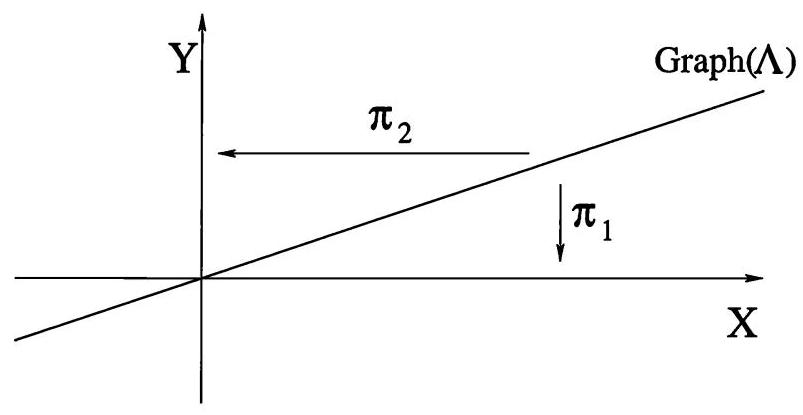
\includegraphics[width=0.65\textwidth]{images/bo_d6ik6nn7aajc739ct1l0_77_338_701_803_415_0.jpg}
\caption{闭图像定理的证明.}
\label{fig:closed-graph-proof}
\end{figure}

\begin{instance}\label{ins:derivative-operator-not-bounded-but-closed}
考虑所有有界连续函数 $f : \mathbb{R} \mapsto  \mathbb{R}$ 构成的空间 $X = {\mathcal{C}}^{0}\left( \mathbb{R}\right)$ ，其范数为 $\| f{\| }_{{\mathcal{C}}^{0}} \doteq  \mathop{\sup }\limits_{x}\left| {f\left( x\right) }\right|$ .令 $\Lambda$ 为由 ${\Lambda f} = {f}^{\prime }$ 定义的微分算子.其定义域为如下子空间
\[
\operatorname{Dom}\left( \Lambda \right)  = \left\{  {f \in  {\mathcal{C}}^{0}\left( \mathbb{R}\right) ;{f}^{\prime } \in  {\mathcal{C}}^{0}\left( \mathbb{R}\right) }\right\}   = {\mathcal{C}}^{1}\left( \mathbb{R}\right)
\]
---即所有导数有界的连续可微函数构成的子空间.

注意，线性算子 $\Lambda$ 不是有界的(因而不连续).例如，函数列 ${f}_{n}\left( x\right)  = \sin {nx}$ 一致有界:对所有 $n \geq  1$ ，均有 ${\norm{f}_{n}}_{{\mathcal{C}}^{0}} = 1$ .然而，其导数序列 $\Lambda {f}_{n} = {f}_{n}^{\prime }$ 无界，因为 ${f}_{n}^{\prime }\left( x\right)  = n\cos {nx}$ ，故 ${\norm{f}_{n}^{\prime }}_{{\mathcal{C}}^{0}} = n$ .

另一方面，线性算子 $\Lambda  : f \mapsto  {f}^{\prime }$ 具有闭图像.为证此，考虑序列 ${f}_{n} \in  \operatorname{Dom}\left( \Lambda \right)$ ，使得对某些函数 $f,g \in  {\mathcal{C}}^{0}$ ，有
\begin{equation}\tag{4.6}\label{eq:derivative-graph-closed}
{\norm{f}_{n} - f}_{{\mathcal{C}}^{0}} \rightarrow  0,\;{\norm{f}_{n}^{\prime } - g}_{{\mathcal{C}}^{0}} \rightarrow  0.
\end{equation}

若\eqref{eq:derivative-graph-closed}成立，则 $f$ 连续可微，且 ${f}^{\prime } = g$ .因此点 $\left( {f,g}\right)  \in  X \times  X$ 属于 $\Lambda$ 的图像.

注意，该例并不与定理\ref{thm:closed-graph}矛盾，因为 $\Lambda$ 并未在整个空间 $X$ 上定义.
\end{instance}

\section{伴随算子}

设 $X$ 是域 $\mathbb{K}$ 上的Banach空间.依定义，其对偶空间是所有有界(因而连续)线性泛函 ${x}^{ * } : X \mapsto  \mathbb{K}$ 构成的空间 ${X}^{ * }$ ，其范数为
\[
\norm{x}^{ * } \doteq  \mathop{\sup }\limits_{{\| x\|  \leq  1}}\left| {{x}^{ * }\left( x\right) }\right| .
\]

反过来，每个元素 $x \in  X$ 均在 ${X}^{ * }$ 上诱导一个有界线性泛函，即 ${x}^{ * } \mapsto  {x}^{ * }\left( x\right)  \in  \mathbb{K}$.利用这一等同关系，我们可写作 $X \subseteq \; {\left( {X}^{ * }\right) }^{ * }$ .由于空间 $X$ 与 ${X}^{ * }$ 常扮演对称角色，采用记号
\[
\left\langle  {{x}^{ * },x}\right\rangle   \doteq  {x}^{ * }\left( x\right) .
\]
设 $X,Y$ 为域 $\mathbb{K}$ 上的Banach空间， ${X}^{ * },{Y}^{ * }$ 为其对偶空间.设 $\Lambda  : X \mapsto  Y$ 为有界线性算子.则对任意有界线性泛函 ${y}^{ * } : Y \mapsto  \mathbb{K}$ ，由 ${x}^{ * } : X \mapsto  \mathbb{K}$ 定义的复合映射 ${x}^{ * }\left( x\right)  = {y}^{ * }\left( {\Lambda x}\right)$ 是 $X$ 上的有界线性泛函.映射 $\Lambda^*:{y}^{ * } \mapsto  {\Lambda }^{ * }{y}^{ * } \doteq  {y}^{ * } \circ  \Lambda$ 是从 ${Y}^{ * }$ 到 ${X}^{ * }$ 的有界线性算子，称为 $\Lambda$ 的伴随算子.\par
\begin{definition}[伴随算子]
    设 $X,Y$ 为域 $\mathbb{K}$ 上的Banach空间， ${X}^{ * },{Y}^{ * }$ 为其对偶空间.设 $\Lambda  : X \mapsto  Y$ 为有界线性算子.则对任意有界线性泛函 ${y}^{ * } : Y \mapsto  \mathbb{K}$ ，由 ${x}^{ * } : X \mapsto  \mathbb{K}$ 定义的复合映射 ${x}^{ * }\left( x\right)  = {y}^{ * }\left( {\Lambda x}\right)$唯一确定$Y^*\to X^*$上的有界线性算子$\Lambda^*:{y}^{ * } \mapsto  {\Lambda }^{ * }{y}^{ * } \doteq  {y}^{ * } \circ  \Lambda$，称为 $\Lambda$ 的\colorbf{伴随算子}.
\end{definition}
根据定义(见图\ref{fig:adjoint-maps})，
\[
\left\langle  {{\Lambda }^{ * }{y}^{ * },x}\right\rangle   = \left\langle  {{y}^{ * },{\Lambda x}}\right\rangle,\;\forall\,x \in  X.
\]

以下，对给定子集 $V \subseteq  X$ ，我们将其正交集定义为
\[
{V}^{ \bot  } \doteq  \left\{  {{x}^{ * } \in  {X}^{ * };\left\langle  {{x}^{ * },x}\right\rangle   = 0,\forall\,x \in  V}\right\}  .
\]

类似地，若 $W \subseteq  {X}^{ * }$ ，我们定义
\[
{W}^{ \bot  } \doteq  \left\{  {x \in  X;\left\langle  {{x}^{ * },x}\right\rangle   = 0,\forall\,{x}^{ * } \in  W}\right\}  .
\]

\begin{figure}[htbp]
\centering
\begin{tikzcd}[labels={font=\normalsize}]
X \arrow[rr, "\Lambda"] &  & Y                            &  & X \arrow[rr, "\Lambda"] \arrow[rrdd, "\Lambda^*y^*"'] &  & Y \arrow[dd, "y^*"] \\
                        &  &                              &  &                                                       &  &                     \\
X^*                     &  & Y^* \arrow[ll, "\Lambda^*"'] &  &                                                       &  & \mathbb{K}         
\end{tikzcd}
\captionof{figure}{伴随算子定义中涉及的映射.}
\label{fig:adjoint-maps}
\end{figure}

\begin{theorem}[伴随算子的性质]\label{thm:adjoint-properties}
设 $\Lambda  : X \mapsto  Y$ 为有界线性算子， ${\Lambda }^{ * } : {Y}^{ * } \mapsto  {X}^{ * }$ 为其伴随算子.则:

(i) $\norm{{\Lambda }^{ * }} = \| \Lambda \|$ .

(ii) $\operatorname{Ker}\left( \Lambda \right)  = {\left(  \operatorname{Range}\left( {\Lambda }^{ * }\right) \right)  }^{ \bot  }$ 且 $\operatorname{Ker}\left( {\Lambda }^{ * }\right)  = {\left(  \operatorname{Range}\left( \Lambda \right) \right)  }^{ \bot  }$ .
\end{theorem}

\begin{proof}
(i) 由下式推出
{\setjot[-2]\begin{align*}
    \| \Lambda \| &= \sup \left\{  {\| {\Lambda x}\| ;\| x\|  \leq  1}\right\}\\
    &= \sup \left\{  {\left| \left\langle  {{y}^{ * },{\Lambda x}}\right\rangle  \right| ;\| x\|  \leq  1,\norm{y}^{ * } \leq  1}\right\}\\
    &= \sup \left\{  {\left| \left\langle  {{\Lambda }^{ * }{y}^{ * },x}\right\rangle  \right| ;\| x\|  \leq  1,\norm{y}^{ * } \leq  1}\right\}\\
    &= \sup \left\{  {\norm{{\Lambda }^{ * }{y}^{ * }};\norm{y}^{ * } \leq  1}\right\}   = \norm{{\Lambda }^{ * }}.
\end{align*}}
(ii) 我们注意到下列命题彼此等价:
{\setjot[-4]\begin{align*}
    x &\in  \operatorname{Ker}\left( \Lambda \right)\\
    {\Lambda x} &= 0 \\
    \left\langle  {{y}^{ * },{\Lambda x}}\right\rangle   &= 0\ \forall\,{y}^{ * } \in  {Y}^{ * } \\
    \left\langle  {{\Lambda }^{ * }{y}^{ * },x}\right\rangle   &= 0\ \forall\,{y}^{ * } \in  {Y}^{ * }   \\
    x &\in  {\left(  \operatorname{Range}\left( {\Lambda }^{ * }\right) \right)  }^{ \bot  }.
\end{align*}}

类似地，下列命题也彼此等价:
{\setjot[-4]\begin{align*}
    {y}^{ * } &\in  \operatorname{Ker}\left( {\Lambda }^{ * }\right)\\
    {\Lambda }^{ * }{y}^{ * } &= 0\\
    \left\langle  {{\Lambda }^{ * }{y}^{ * },x}\right\rangle   &= 0\ \forall\,x \in  X\\
    \left\langle  {{y}^{ * },{\Lambda x}}\right\rangle   &= 0\ \forall\,x \in  X\\
    {y}^{ * } &\in  {\left(  \operatorname{Range}\left( \Lambda \right) \right)  }^{ \bot  }.
\end{align*}}

\end{proof}

本节最后，我们给出一致有界性原理的一个有用应用.

\begin{corollary}[弱收敛序列必有界]\label{cor:weakly-convergent-bounded}
设 $X$ 为Banach空间，则任何弱收敛于某个 $x \in  X$ 的序列 ${x}_{n} \in  X$ 必为有界序列.
\end{corollary}

\begin{proof}
设 ${X}^{ * }$ 为 $X$ 的对偶空间.每个 ${x}_{n}$ 确定 ${X}^{ * }$ 上的一个线性泛函 ${\psi }_{n}$ ，定义为
\[
{\psi }_{n}\left( {x}^{ * }\right)  \doteq  \left\langle  {{x}^{ * },{x}_{n}}\right\rangle  .
\]
此处 $\langle  \cdot  , \cdot  \rangle$ 表示 $X$ 与 ${X}^{ * }$ 之间的对偶关系.由假设，当 $n \rightarrow  \infty$ 时，逐点收敛
\[
{\psi }_{n}\left( {x}^{ * }\right)  =  \left\langle  {{x}^{ * },{x}_{n}}\right\rangle   \rightarrow  \left\langle  {{x}^{ * },x}\right\rangle
\]
对每个 ${x}^{ * } \in  {X}^{ * }$ 成立.这意味着
\[
\mathop{\sup }\limits_{n}\left| {{\psi }_{n}\left( {x}^{ * }\right) }\right|  < \infty \text{ for every }{x}^{ * } \in  {X}^{ * }.
\]

由定理\ref{thm:banach-steinhaus}可知，线性泛函族 $\left\{  {{\psi }_{n};n \geq  1}\right\}$ 一致有界.又因
\[
\norm{{\psi }_{n}} = \mathop{\sup }\limits_{{\norm{x}^{ * } \leq  1}}\left| {{\psi }_{n}\left( {x}^{ * }\right) }\right|  = \norm{{x}_{n}},
\]
故序列 ${x}_{n}$ 有界.
\end{proof}

\section{紧算子}

\begin{definition}[紧算子]
    设 $X,Y$ 为Banach空间.称有界线性算子 $\Lambda  : X \mapsto  Y$ 为\colorbf{紧算子}，若其满足任一等价条件：
    \begin{enumerate}[(i)]
        \item 对 $X$ 中任意有界点列 ${\left( {x}_{n}\right) }_{n \geq  1}$ ，均存在子列 ${\left( {x}_{{n}_{j}}\right) }_{j \geq  1}$ ，使得 $\Lambda {x}_{{n}_{j}}$ 收敛.
        \item 对 $X$ 中任意有界集 $U$ ，其像 $\Lambda \left( U\right)$ 的闭包 $\overline{\Lambda \left( U\right) }$ 是 $Y$ 中的紧集.
    \end{enumerate}
\end{definition}


\begin{theorem}[紧算子的例子]\label{thm:compact-examples}
(i) 设 $X,Y$ 为Banach空间， $\Lambda  : X \mapsto  Y$ 为有界线性算子.若 $\Lambda$ 的值域是有限维的，则 $\Lambda$ 是紧算子.

(ii) 设 ${\Lambda }_{n} : X \mapsto  Y$ 为紧算子，对每个 $n \geq  1$ 成立.假设 $\mathop{\lim }\limits_{{n \rightarrow  \infty }}\norm{{\Lambda }_{n} - \Lambda } = 0$ .则算子 $\Lambda$ 也是紧的.
\end{theorem}

\begin{proof}
1. 有界线性算子 $\Lambda  : X \mapsto  Y$ 是紧的当且仅当单位球 ${B}_{1} \subset  X$ 的像 $\Lambda \left( {B}_{1}\right)  \subset  Y$ 的闭包是紧的.若 $\operatorname{Range}\left( \Lambda \right)$ 是有限维的且 $\Lambda$ 有界，则闭包 $\overline{\Lambda \left( {B}_{1}\right) }$ 是有限维空间中的闭有界子集，故为紧集.这就证明了 (i).

\noindent 2. 为证 (ii)，我们注意到:由于 $Y$ 完备，闭包 $\overline{\Lambda \left( {B}_{1}\right) }$ 是紧的当且仅当 $\Lambda \left( {B}_{1}\right)$ 是列紧的.这意味着:对任意 $\varepsilon  > 0$ ，集合 $\Lambda \left( {B}_{1}\right)$ 可被有限个半径为 $\varepsilon$ 的球覆盖.

在假设 (ii) 下，给定 $\varepsilon  > 0$ .选取 $k$ 使得 $\norm{\Lambda  - {\Lambda }_{k}} < \varepsilon /2$ .由于 ${\Lambda }_{k}$ 是紧的，可选出有限个元素 ${y}_{1},\ldots ,{y}_{N} \in  Y$ ，使得
\begin{equation}\tag{4.7}\label{eq:compact-covering}
{\Lambda }_{k}\left( {B}_{1}\right)  \subseteq  \mathop{\bigcup }\limits_{{i = 1}}^{N}B\left( {{y}_{i},\frac{\varepsilon }{2}}\right) .
\end{equation}

若 $\| x\|  \leq  1$ ，则 $\norm{{\Lambda x} - {\Lambda }_{k}x} < \varepsilon /2$ .由\eqref{eq:compact-covering}存在一点 ${y}_{i}$ 满足 $\norm{{\Lambda }_{k}x - {y}_{i}} < \varepsilon /2$ .由三角不等式， $\norm{{\Lambda x} - {y}_{i}} < \varepsilon$ .这表明有限个球 $B\left( {{y}_{i},\varepsilon }\right)$ 覆盖了 $\Lambda \left( {B}_{1}\right)$ .
\end{proof}

\begin{theorem}[紧算子的伴随算子]\label{thm:compact-adjoint}
设 $X,Y$ 为Banach空间， $\Lambda  : X \mapsto  Y$ 为有界线性算子.则 $\Lambda$ 是紧算子当且仅当其伴随算子 ${\Lambda }^{ * } : {Y}^{ * } \mapsto  {X}^{ * }$ 是紧算子.
\end{theorem}

\begin{proof}
1. 假设 $\Lambda$ 是紧算子.设 ${\left( {y}_{n}^{ * }\right) }_{n \geq  1}$ 是 ${Y}^{ * }$ 中的一列，且对每个 $n$ 均有 $\norm{{y}_{n}^{ * }} \leq  1$ .为证 ${\Lambda }^{ * }$ 是紧算子，需证序列 ${\left( {\Lambda }^{ * }{y}_{n}^{ * }\right) }_{n \geq  1}$ 存在收敛子列.

令 ${B}_{1} \doteq  \{ x \in  X;\| x\|  \leq  1\}$ 为 $X$ 中的闭单位球.由假设，像集 $\Lambda \left( {B}_{1}\right)$ 具有紧闭包，记作 $E \doteq  \overline{\Lambda \left( {B}_{1}\right) } \subset  Y.$

\noindent 2. 依定义，每个 ${y}_{n}^{ * } \in  {Y}^{ * }$ 均为从 $Y$ 到域 $\mathbb{K}$ 的线性映射.令 ${f}_{n} : E \mapsto  \mathbb{K}$ 为 ${y}_{n}^{ * }$ 在紧集 $E$ 上的限制.我们断言函数族 $\left\{  {{f}_{n};n \geq  1}\right\}$ 满足Ascoli定理的条件.事实上，所有这些函数一致Lipschitz连续，因为
\[
\left| {{f}_{n}\left( y\right)  - {f}_{n}\left( {y}^{\prime }\right) }\right|  \leq  \norm{{y}_{n}^{ * }}\norm{y - {y}^{\prime }} \leq  \norm{y - {y}^{\prime }},\;\forall\,y,{y}^{\prime } \in  E.
\]

此外，注意到
\[
\mathop{\sup }\limits_{{y \in  E}}\| y\|  = \mathop{\sup }\limits_{{\| x\|  \leq  1}}\| {\Lambda x}\|  = \| \Lambda \|
\]
可得
\[
\left| {{f}_{n}\left( y\right) }\right|  \leq  \norm{{y}_{n}^{ * }}\| y\|  \leq  1 \cdot  \| \Lambda \| ,\;\forall\,y \in  E.
\]
因此所有函数 ${f}_{n} : E \mapsto  \mathbb{K}$ 一致有界.

由定理\ref{thm:ascoli}，存在子列 ${\left( {f}_{{n}_{j}}\right) }_{j \geq  1}$ ，其在紧集 $E = \overline{\Lambda \left( {B}_{1}\right) }$ 上一致收敛于某函数 $f$ .

\noindent 3. 我们现观察到
{\begin{align*}
    \norm{{\Lambda }^{ * }{y}_{{n}_{i}}^{ * } - {\Lambda }^{ * }{y}_{{n}_{j}}^{ * }} &= \mathop{\sup }\limits_{{\| x\|  \leq  1}}\left| \left\langle  {{\Lambda }^{ * }{y}_{{n}_{i}}^{ * } - {\Lambda }^{ * }{y}_{{n}_{j}}^{ * },x}\right\rangle  \right|\\
    &= \mathop{\sup }\limits_{{\| x\|  \leq  1}}\left| \left\langle  {{y}_{{n}_{i}}^{ * } - {y}_{{n}_{j}}^{ * },{\Lambda x}}\right\rangle  \right|  = \mathop{\sup }\limits_{{\| x\|  \leq  1}}\left| {{f}_{{n}_{i}}\left( {\Lambda x}\right)  - {f}_{{n}_{j}}\left( {\Lambda x}\right) }\right| ,
\end{align*}}

其中右端当 $i,j \rightarrow  \infty$ 时趋于零.这表明子列 ${\left( {\Lambda }^{ * }{y}_{{n}_{j}}^{ * }\right) }_{j \geq  1}$ 是Cauchy列，故必收敛于某极限 ${x}^{ * } \in  {X}^{ * }$ .因此 ${\Lambda }^{ * }$ 是紧算子.

反之亦然，可用相同论证证明.
\end{proof}

\vspace{-0.3 em}
\subsection{积分算子}

紧算子常以积分算子形式出现.举例而言，考虑Banach空间 $\mathcal{C}\left( \left(  {a,b}\right)  \right)$ ，即定义在闭区间 $\left(  {a,b}\right)$ 上所有连续实值函数构成的空间.
\vspace{1 em}
\begin{theorem}[积分算子的紧性]\label{thm:integral-operator-compact}
设 $K : \left(  {a,b}\right)   \times \; \left(  {a,b}\right)   \mapsto  \mathbb{R}$ 是连续映射.则积分算子
\begin{equation}\tag{4.8}\label{eq:integral-operator-def}
\left( {\Lambda f}\right) \left( x\right)  \doteq  {\int }_{a}^{b}K\left( {x,y}\right) f\left( y\right) {dy}
\end{equation}
是从 $\mathcal{C}\left( \left(  {a,b}\right)  \right)$ 到自身的紧线性算子.
\end{theorem}

\begin{proof}
考虑一列有界连续函数 ${f}_{n} \in  \mathcal{C}\left( \left(  {a,b}\right)  \right)$ .需证序列 $\Lambda {f}_{n}$ 存在一致收敛子列.由定理\ref{thm:ascoli}，只需证函数 $\Lambda {f}_{n}$ 一致有界且等度连续.

1. 由于 $K$ 在紧集 $\left(  {a,b}\right)   \times  \left(  {a,b}\right)$ 上连续，故有界且一致连续.即存在常数 $\kappa$ 使得
\[
\left| {K\left( {x,y}\right) }\right|  \leq  \kappa \;\forall\,x,y.
\]

此外，对每个 $\varepsilon  > 0$ ，存在 $\delta  > 0$ 使得
\begin{equation}\tag{4.9}\label{eq:kernel-uniform-cont}
\left| {K\left( {x,y}\right)  - K\left( {\widetilde{x},y}\right) }\right| \; \leq  \;\varepsilon ,\;\text{当}\;\left| {x - \widetilde{x}}\right|  \leq  \delta ,\;x,\widetilde{x},y \in  \left(  {a,b}\right)  .
\end{equation}

\noindent 2. 由假设，存在常数 $M$ 使得
\[
\norm{f}_{n}\; = \;\mathop{\max }\limits_{{x \in  \left(  {a,b}\right)  }}\left| {{f}_{n}\left( x\right) }\right| \; \leq  \;M,\;\forall\,\;n \geq  1\;.
\]

这意味着
\[
\left| {\left( {\Lambda {f}_{n}}\right) \left( x\right) }\right|  \leq  {\int }_{a}^{b}\left| {K\left( {x,y}\right) }\right| \left| {{f}_{n}\left( y\right) }\right| {dy} \leq  \left( {b - a}\right) {\kappa M},
\]
证明了函数 $\Lambda {f}_{n}$ 一致有界.

\noindent 3. 接下来，设 $\varepsilon  > 0$ 给定.选取 $\delta  > 0$ 使得\eqref{eq:kernel-uniform-cont}成立.若 $\left| {x - \widetilde{x}}\right|  \leq  \delta$ ，则对任意 $n \geq  1$ ，有
\[
\left| {\left( {\Lambda {f}_{n}}\right) \left( x\right)  - \left( {\Lambda {f}_{n}}\right) \left( \widetilde{x}\right) }\right| \; \leq  \;{\int }_{a}^{b}\left| {K\left( {x,y}\right)  - K\left( {\widetilde{x},y}\right) }\right| \left| {{f}_{n}\left( y\right) }\right| {dy}\; \leq  \;\left( {b - a}\right) {\varepsilon M}.
\]

由于 $\varepsilon  > 0$ 是任意的，这证明了序列 ${\left( \Lambda {f}_{n}\right) }_{n \geq  1}$ 的等度连续性.应用定理\ref{thm:ascoli}即完成证明.
\end{proof}

\begin{figure}[htbp]
\centering
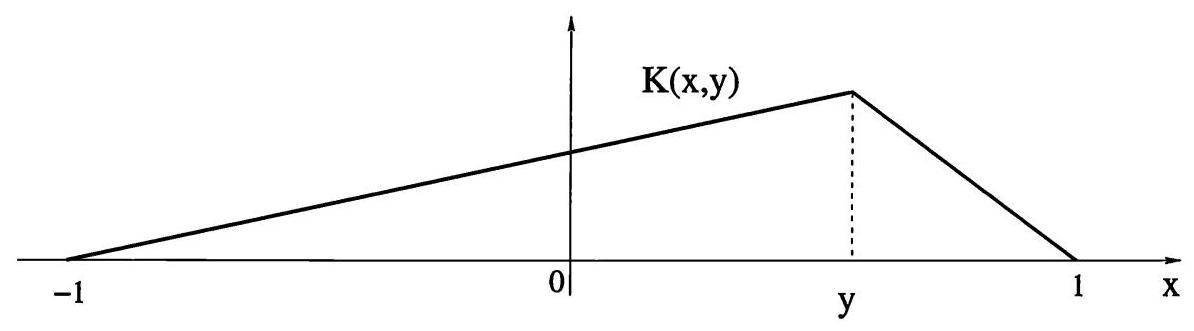
\includegraphics[width=1.0\textwidth]{images/bo_d6ik6nn7aajc739ct1l0_83_147_230_1194_331_0.jpg}
\caption{式\eqref{eq:green-kernel}中的核函数 $K$.}
\label{fig:kernel-function-K}
\end{figure}

\begin{instance}\label{ins:two-point-bvp-compact}
对任意连续函数 $f \in  \mathcal{C}\left( \left(  {-1,1}\right)  \right)$ ，令 $u = {\Lambda f}$ 为两点边值问题的解
\begin{equation}\tag{4.10}\label{eq:two-point-bvp}
{u}^{\prime \prime }\left( x\right)  + f\left( x\right)  = 0,\;u\left( {-1}\right)  = u\left( 1\right)  = 0.
\end{equation}

注意解必唯一.事实上，若 ${u}_{1},{u}_{2}$ 均为解，则函数 $w = {u}_{1} - {u}_{2}$ 满足
\[
{w}^{\prime \prime }\left( x\right)  = 0,\;w\left( {-1}\right)  = w\left( 1\right)  = 0,
\]
故 $w\left( x\right)  \equiv  0$ .直接计算表明
\[
u\left( x\right)  = {\int }_{-1}^{x}\frac{\left( {1 + y}\right) \left( {1 - x}\right) }{2}f\left( y\right) {dy} + {\int }_{x}^{1}\frac{\left( {1 - y}\right) \left( {1 + x}\right) }{2}f\left( y\right) {dy}
\]
给出了\eqref{eq:two-point-bvp}的一个解.因此解算子 $\Lambda  : f \mapsto  u = {\Lambda f}$ 是 $\mathcal{C}\left( \left(  {-1,1}\right)  \right)$ 上的线性紧算子.它可写成\eqref{eq:integral-operator-def}的形式，其中
\begin{equation}\tag{4.11}\label{eq:green-kernel}
K\left( {x,y}\right)  \doteq \begin{cases}\frac{\left( {1 - y}\right) \left( {1 + x}\right) }{2} & \text{ if } - 1 \leq  x \leq  y, \\[5pt]  \frac{\left( {1 + y}\right) \left( {1 - x}\right) }{2} & \text{ if }y \leq  x \leq  1. \end{cases}
\end{equation}

参照图\ref{fig:kernel-function-K}，对固定 $y$ ，分段仿射映射 $x \mapsto  K\left( {x,y}\right)$ 可由以下三个方程唯一确定
\[
K\left( {-1,y}\right)  = K\left( {1,y}\right)  = 0,\;{K}_{x}\left( {y+,y}\right)  - {K}_{x}\left( {y-,y}\right)  =  - 1.
\]
\end{instance}

\section{习题}

\begin{rbhw}[index=1]
在Banach空间 $X = \mathcal{C}\left( \left(  {0,1}\right)  \right)$ 上，判断下列算子是否(i)线性、(ii)有界、(iii)紧:

(1) $\left( {\Lambda f}\right) \left( x\right)  = f\left( {\sin x}\right)$ .

(2) $\left( {\Lambda f}\right) \left( x\right)  = \sin \left( {f\left( x\right) }\right)$ .

(3) $\left( {\Lambda f}\right) \left( x\right)  = {xf}\left( x\right)$ .

(4) $\left( {\Lambda f}\right) \left( x\right)  = {xf}\left( 0\right)  + {\int }_{0}^{1}f\left( s\right) {ds}$ .

(5) $\left( {\Lambda f}\right) \left( x\right)  = y\left( x\right)$ ，其中 $y\left( \cdot \right)$ 是Cauchy问题的解
\[
{y}^{\prime }\left( x\right)  + y\left( x\right)  = f\left( x\right) ,\;y\left( 0\right)  = 0.
\]
\end{rbhw}

\begin{rbhw}
证明 ${L}^{2}\left( \left(  {0,1}\right)  \right)$ 是 ${L}^{1}\left( \left(  {0,1}\right)  \right)$ 中第一纲的向量子空间.事实上，对每个 $n \geq  1$ ，集合 ${E}_{n} \doteq  \left\{  {f : \left(  {0,1}\right)   \mapsto  \mathbb{R};{\int }_{0}^{1}{\left| f\right| }^{2}{dx} \leq  n}\right\}$ 是 ${L}^{1}$ 中无内点的闭子集.
\end{rbhw}

\begin{rbhw}
设 $X$ 为一个 Banach 空间， $\Lambda  : X \mapsto  {\ell }^{\infty }$ 为一线性算子，使得对每个 $x \in  X$ ， $\Lambda \left( x\right)  = \left( {{\Lambda }_{1}\left( x\right) ,{\Lambda }_{2}\left( x\right) ,\ldots }\right)$ 均为一有界实数列.证明:算子 $\Lambda$ 有界当且仅当每个线性泛函 ${\Lambda }_{n}$ 有界.
\end{rbhw}

\begin{rbhw}
设 $1 \leq  p \leq  \infty$ .考虑定义在整个空间 ${L}^{p}$ 上的线性算子 $\Lambda  : {L}^{p}\left( \left(  {0,1}\right)  \right)  \mapsto  {L}^{p}\left( \left(  {0,1}\right)  \right)$ ，其具有如下性质:若函数列 ${f}_{n} \in  {L}^{p}$ 几乎处处点态收敛于某个 $f \in  {L}^{p}$，则序列 $\left( {\Lambda {f}_{n}}\right) \left( x\right)$ 几乎处处收敛于 $\left( {\Lambda f}\right) \left( x\right)$ (对几乎所有的 $x \in  \left(  {0,1}\right)$ ).证明: $\Lambda$ 连续.
\end{rbhw}

\begin{rbhw}
设 $X$ 为无限维 Banach 空间， $K : X \mapsto  X$ 为一紧线性算子.若 $K$ 是单射，则 $K$ 的值域不可能是闭的.
\end{rbhw}

\begin{rbhw}
设 $X,Y,Z$ 为 Banach 空间，考虑两个线性算子 ${\Lambda }_{1} : X \mapsto \; Y,{\Lambda }_{2} : Y \mapsto  Z$ .假设其中一算子连续，另一算子紧.证明:复合算子 ${\Lambda }_{2} \circ  {\Lambda }_{1} : X \mapsto  Z$ 为紧线性算子.
\end{rbhw}

\begin{rbhw}
设 $X$ 为 Banach 空间， $\Lambda  : X \mapsto  X$ 为满足 $\Lambda  = {\Lambda }^{2}$ 的紧线性算子，即对所有 $x \in  X$ ，均有 $\Lambda \left( x\right)  = \Lambda \left( {\Lambda \left( x\right) }\right)$ .证明: $\operatorname{Range}\left( \Lambda \right)$ 是有限维的.
\end{rbhw}

\begin{rbhw}
设 $X$ 为 Banach 空间， $U \subset  X$ 为一闭凸集，且满足 $\mathop{\bigcup }\limits_{{n \geq  1}}{nU} = X$ .证明: $U$ 包含原点的一个邻域.
\end{rbhw}

\begin{rbhw}
设 $X,Y$ 为无限维 Banach 空间.若 $K : X \mapsto  Y$ 为紧线性算子，则 $K\left( X\right)  \neq  Y$ ，即 $K$ 不可能是满射.

例如，考虑如下定义的映射 $K : {\ell }^{1} \mapsto  {\ell }^{1}$ :若 $\bm{x} = \; \left( {{x}_{1},{x}_{2},{x}_{3},\ldots }\right)$ 且 $\| \bm{x}{\| }_{{\ell }^{1}} \doteq  \mathop{\sum }\limits_{{n \geq  1}}\left| {x}_{n}\right|  < \infty$ ，则 $K\bm{x} = \left( {\frac{{x}_{1}}{1},\frac{{x}_{2}}{2},\frac{{x}_{3}}{3},\ldots ,\frac{{x}_{n}}{n},\ldots }\right)$ .求一点 $\bm{y} \in  {\ell }^{1} \setminus  K\left( {\ell }^{1}\right)$ .
\end{rbhw}

\begin{rbhw}
设 $f : \mathbb{R} \mapsto  \mathbb{R}$ 是一个具有闭图像的有界函数.证明 $f$ 连续.

另一方面，构造一个单射且满射、具有闭图像但不连续的函数 $g : \mathbb{R} \mapsto  \mathbb{R}$ .
\end{rbhw}

\begin{rbhw}
设 $X,Y$ 是Banach空间.证明每个连续函数 $f : X \mapsto  Y$ (未必是线性的)均具有闭图像.

构造一个具有闭图像但不连续的有界函数 $g : \mathbb{R} \mapsto  {L}^{1}\left( \mathbb{R}\right)$ .
\end{rbhw}

\begin{rbhw}
设 $1 \leq  p < \infty$ ，并考虑所有实数列 $\bm{x} = \; \left( {{x}_{1},{x}_{2},{x}_{3},\ldots }\right)$ 构成的Banach空间 ${\ell }^{p}$，其中满足 $\| \bm{x}{\| }_{p} \doteq  {\left( \mathop{\sum }\limits_{{k \geq  1}}{\left| {x}_{k}\right| }^{p}\right) }^{1/p} < \infty$ .设 $\left( {{\lambda }_{1},{\lambda }_{2},{\lambda }_{3},\ldots }\right)$ 是一有界实数列，并定义有界线性算子 $\Lambda  : {\ell }^{p} \mapsto  {\ell }^{p}$ 如下:

\[
\Lambda \left( {{x}_{1},{x}_{2},{x}_{3},\ldots }\right)  \doteq  \left( {{\lambda }_{1}{x}_{1},{\lambda }_{2}{x}_{2},{\lambda }_{3}{x}_{3},\ldots }\right) .
\]

证明: $\Lambda$ 是紧算子当且仅当 $\mathop{\lim }\limits_{{k \rightarrow  \infty }}{\lambda }_{k} = 0$ .
\end{rbhw}

\begin{rbhw}
设 $X,Y,Z$ 为Banach空间， $B : X \times  Y \mapsto  Z$ 为双线性映射\footnote{称 $B$ 是双线性的，是指:对每个给定的 $y \in  Y$ ， $x \mapsto  B\left( {x,y}\right)$ 是线性映射；且对每个固定的 $x \in  X$ ， $y \mapsto  B\left( {x,y}\right)$ 是线性映射.}.假设 $B$ 在原点处连续.证明: $B$ 是有界的；即存在常数 $C$ ，使得
\[
\| B\left( {x,y}\right) \|  \leq  C\| x\| \| y\| \;\forall\,x \in  X,y \in  Y.
\]

\end{rbhw}

\begin{rbhw}
设 $X$ 为所有一元实变量多项式构成的向量空间，其范数为
\[
\| p\|  \doteq  {\int }_{0}^{1}\left| {p\left( t\right) }\right| {\d t}
\]
考虑如下定义的双线性泛函 $B : X \times  X \mapsto  \mathbb{R}$ :
\[
B\left( {p,q}\right)  = {\int }_{0}^{1}p\left( t\right) q\left( t\right) {\d t}
\]
证明:对每个固定的 $p \in  X$ ，映射 $q \mapsto  B\left( {p,q}\right)$ 是 $X$ 上的连续线性泛函；类似地，对固定的 $q \in  X$ ，映射 $p \mapsto  B\left( {p,q}\right)$ 是连续线性泛函.然而，证明 $B$ 并非从积空间 $X \times  X$ 到 $\mathbb{R}$ 的连续映射.我们回顾: $X \times  X$ 具有范数 $\| \left( {p,q}\right) \|  \doteq  \max \left\{  {{\int }_{0}^{1}\left| {p\left( x\right) }\right| {dx},{\int }_{0}^{1}\left| {q\left( x\right) }\right| {dx}}\right\}$ .
\end{rbhw}

\begin{rbhw}
设 $S$ 是Banach空间 $X$ 中的一个闭有界子集.假设对每个 $\varepsilon  > 0$ ，均存在一个有限维子空间 ${Y}_{\varepsilon } \subseteq  X$ ，使得
\[
d\left( {S,{Y}_{\varepsilon }}\right)  \doteq  \mathop{\sup }\limits_{{x \in  S}}d\left( {x,{Y}_{\varepsilon }}\right)  \leq  \varepsilon
\]
证明:集合 $S$ 是紧集.
\end{rbhw}

\begin{rbhw}
设 $A$ 是Banach空间 $X$ 上的有界线性算子.若对每个紧算子 $K$ 均有 ${AK} = {KA}$，则证明 $A$ 是恒等算子的标量倍数，即存在某个数 $\lambda$ ，使得 $A = {\lambda I}$ .
\end{rbhw}


\begin{rbhw}
设 $X$ 是Banach空间， $\Lambda  : X \mapsto  X$ 是其上有界线性算子.假设存在 $\varepsilon  > 0$ 及一个无限维子空间 $V \subseteq  X$ ，使得对每个 $x \in  V$ 均有 $\| {\Lambda x}\|  \geq  \varepsilon \| x\|$ .证明:算子 $\Lambda$ 不可能是紧算子.
\end{rbhw}

\begin{rbhw}
设 $X$ 为 Banach 空间， ${X}^{ * }$ 为其对偶空间.考虑一列元素 ${x}_{k} \in  X$ ，满足级数 $\mathop{\sum }\limits_{{k > 1}}\left\langle  {{x}^{ * },{x}_{k}}\right\rangle$ 对每个 ${x}^{ * } \in  {X}^{ * }$ 均收敛.证明
\[
{x}^{ * } \mapsto  \varphi \left( {x}^{ * }\right)  \doteq  \mathop{\sum }\limits_{{k \geq  1}}\left\langle  {{x}^{ * },{x}_{k}}\right\rangle
\]
是 ${X}^{ * }$ 上的有界线性泛函.
\end{rbhw}

\begin{rbhw}
在 Banach 空间 $X = \mathcal{C}\left( \left(  {0,1}\right)  \right)$ 上，考虑由下式定义的线性算子 $\Lambda  : X \mapsto  X$ :
\[
\left( {\Lambda f}\right) \left( 0\right)  = f\left( 0\right) ,\;\left( {\Lambda f}\right) \left( t\right)  = \frac{1}{t}{\int }_{0}^{t}f\left( s\right) {ds}\;\text{ for }t > 0.
\]
(i) 证明 $\Lambda$ 连续.

(ii) 证明 $\Lambda$ 是单射但不是满射.

(iii) 证明 $\Lambda$ 不是紧算子.
\end{rbhw}

\begin{rbhw}
设 $\Omega  \subset  {\mathbb{R}}^{n}$ 为开集， $g : \Omega  \mapsto  \mathbb{R}$ 为有界可测函数.仿照例 2.18，对任意 $1 \leq  p \leq  \infty$，在空间 ${L}^{p}\left( \Omega \right)$ 上考虑乘法算子 $\left( {{M}_{g}f}\right) \left( x\right)  \doteq  g\left( x\right) f\left( x\right)$ .

(i) 确定使算子 ${M}_{g}$ 为单射的函数 $g$ .

(ii) 确定使算子 ${M}_{g}$ 具有闭值域的函数 $g$ .

(iii) 确定使算子 ${M}_{g}$ 为紧算子的函数 $g$ .
\end{rbhw}

\begin{rbhw}
构造一个例子，说明:对无穷维 Banach 空间 $X$ ，所有单射的有界线性算子 $\Lambda  : X \mapsto  X$ 的集合未必是全体有界线性算子空间 $\mathcal{B}\left( {X;X}\right)$ 中的开集.

类似地，说明值域稠密的有界线性算子集合在 $\mathcal{B}\left( {X;X}\right)$ 中也未必是开集.
\end{rbhw}

\begin{rbhw}
设 $X,Y$ 为 Banach 空间， $\Lambda  : X \mapsto  Y$ 为连续线性双射.

(i) 证明存在 $\beta  > 0$ ，使得
\[
\| {\Lambda x}\|  \geq  \beta \| x\| \forall\,x \in  X.
\]

(ii) 设 $\Psi  \in  \mathcal{B}\left( {X;Y}\right)$ 为任一范数为 $\| \Psi \|  < \beta$ 的有界线性算子.利用压缩映射原理，证明:对任意 $f \in  Y$ ，方程
\[
u = {\Lambda }^{-1}\left( {f - {\Psi u}}\right)
\]
有唯一解.

(iii) 证明:在Banach空间 $\mathcal{B}\left( {X;Y}\right)$ 中，所有双射算子构成的集合是开集.
\end{rbhw}

\begin{rbhw}
回顾第2章例2.6与2.7中引入的空间，定义算子 $\Lambda  : {\ell }^{\infty } \mapsto  {\ell }^{\infty }$ 如下: ${\Lambda x} = y = \left( {{y}_{1},{y}_{2},{y}_{3},\ldots }\right)$ ，其中
\begin{equation}\tag{4.12}\label{eq:cesaro-mean}
{y}_{n} \doteq  \frac{1}{n}\mathop{\sum }\limits_{{i = 1}}^{n}{x}_{i}
\end{equation}

(i) 证明 $\Lambda$ 是有界线性算子，并计算其范数. $\Lambda$ 是紧算子吗？

(ii) 考虑如式\eqref{eq:cesaro-mean}所定义的算子 $\Lambda$ ，但作用于绝对可和序列空间 ${\ell }^{1}$ 上. $\Lambda$ 是有界线性算子吗？它是否紧？
\end{rbhw}

\begin{rbhw}
设 $X,Y$ 为向量空间，且 $Y \subseteq  X$ .假设存在范数，使得 $\left( {X\;;\;\|  \cdot  {\| }_{X}}\right)$ 与 $\left( {Y\;;\;\|  \cdot  {\| }_{Y}}\right)$ 均为Banach空间，且满足
\[
\| y{\| }_{X} \leq  C \cdot  \| y{\| }_{Y}\;\forall\,y \in  Y.
\]

(i) 若 $Y = X$ ，证明两种范数 $\|  \cdot  {\| }_{X}$ 与 $\|  \cdot  {\| }_{Y}$ 等价，即存在常数 ${C}^{\prime }$ ，使得 $\| x{\| }_{Y} \leq  {C}^{\prime } \cdot  \| x{\| }_{X}$ .

(ii) 若 $Y \neq  X$ ，证明 $Y$ 是 $X$ 中的第一纲集.即每个集合 ${S}_{n} \doteq  \left\{  {y \in  Y;\| y{\| }_{Y} \leq  n}\right\}$ 均为 $X$ 的闭集且无处稠密.
\end{rbhw}


\chapter{Hilbert空间}\vspace{-2em}

欧几里得空间 ${\mathbb{R}}^{n}$ 配备了自然的内积 $\langle  \cdot  , \cdot  \rangle$ .该内积具有多方面用途:

\begin{itemize}
\item 它定义了欧几里得范数 $\| \bm{x}\|  \doteq  \sqrt{\langle \bm{x},\bm{x}\rangle }$ .
\item 它确定了正交空间与正交投影，并允许我们构造彼此正交的向量基 $\left\{  {{\bm{v}}_{1},\ldots ,{\bm{v}}_{n}}\right\}$.得益于内积，计算向量 $\bm{v} \in  {\mathbb{R}}^{n}$ 关于正交基的分量变得十分简便.
\item 每个线性泛函 $\varphi  : {\mathbb{R}}^{n} \mapsto  \mathbb{R}$ 均可表示为内积形式: $\varphi \left( \bm{x}\right)  = \langle \bm{w},\bm{x}\rangle$ ，其中 $\bm{w} \in  {\mathbb{R}}^{n}$ 为某个适当的向量.
\item 有了内积，便可定义一类对称算子，其具有诸多良好性质.我们回顾:若对所有 $x,y \in  {\mathbb{R}}^{n}$ 均有 $\langle A\bm{x},\bm{y}\rangle  = \langle \bm{x},A\bm{y}\rangle$ ，则称 $A : {\mathbb{R}}^{n} \mapsto  {\mathbb{R}}^{n}$ 为对称算子.在 ${\mathbb{R}}^{n}$ 的标准基下，对称算子对应于对称 $n \times  n$ 矩阵.
\item 始终依赖内积，可定义一类正算子.我们回顾:若对所有 $\bm{x} \in  {\mathbb{R}}^{n},\bm{x} \neq  0$ 均有 $\langle A\bm{x},\bm{x}\rangle  > 0$ ，则 $A : {\mathbb{R}}^{n} \mapsto  {\mathbb{R}}^{n}$ 是严格正定的.此时，映射 $\bm{x} \mapsto  \langle A\bm{x},\bm{x}\rangle$ 是一个正定二次型.
\end{itemize}

本章目标是展示欧几里得内积的定义与性质如何推广至无限维向量空间.

\section{具有内积的空间}

\begin{definition}[内积空间]
    设 $H$ 是域 $\mathbb{K}$ (实数域或复数域)上的向量空间，$H$ 上的一个内积是指映射 $\left( {\cdot , \cdot  }\right):H\times H\to\mathbb{K}$，并满足如下性质:对任意 $x,y,z \in  H$ 与 $\alpha  \in  \mathbb{K}$ ，均有
    \begin{enumerate}[(i)]
        \item  $\left( {x,y}\right)  = \overline{\left( y,x\right) }$ ，其中上横线表示复共轭；
        \item $\left( {x + y,z}\right)  = \left( {x,z}\right)  + \left( {y,z}\right)$ ；
        \item $\left( {{\alpha x},z}\right)  = \alpha \left( {x,z}\right)$
        \item $\left( {x,x}\right)  \geq  0$ ，且等号成立当且仅当 $x = 0$ .
    \end{enumerate}
\end{definition}



注意，上述性质还蕴含
\begin{equation}\tag{5.1}\label{eq:inner-product-linearity}
\left( {x,y + z}\right)  = \left( {x,y}\right)  + \left( {x,z}\right) ,\;\left( {x,{\alpha y}}\right)  = \overline{\alpha }\left( {x,y}\right) .
\end{equation}

当 $\mathbb{K} = \mathbb{R}$ 时，性质 (i)-(iii) 单纯表明:实向量空间上的内积是一个对称双线性映射.关联上述内积，我们还定义
\begin{equation}\tag{5.2}\label{eq:norm-from-inner-product}
\| x\|  \doteq  \sqrt{\left( x,x\right) }.
\end{equation}

后文证明的Minkowski不等式表明，这确为向量空间 $H$ 上的一个范数.

\begin{theorem}[两个基本不等式]\label{thm:basic-inequalities}
设 $H$ 是具有内积 $\left( {\cdot , \cdot  }\right)$ 的向量空间，则

(i) $\left| \left( {x,y}\right) \right|  \leq  \| x\| \| y\| \;$ (Cauchy-Schwartz不等式)；

(ii) $\| x + y\|  \leq  \| x\|  + \| y\| \;$ (Minkowski不等式).
\end{theorem}

\begin{proof}
(i) 若 $y = 0$ ，第一个不等式显然成立.为涵盖一般情形，令
\[
a \doteq  \left( {x,x}\right) ,\;b \doteq  \left( {x,y}\right) ,\;c \doteq  \left( {y,y}\right) .
\]

对任一标量 $\lambda  \in  \mathbb{K}$ ，均有
\[
0 \leq  \left( {x + {\lambda y},x + {\lambda y}}\right)  = a + b\overline{\lambda } + \bar{b}\lambda  + {c\lambda }\overline{\lambda }.
\]

取 $\lambda  =  - b/c$ ，得
\[
0 \leq  a - \frac{b\bar{b}}{c}.
\]

由于 $c = \left( {y,y}\right)  > 0$ ，两边同乘 $c$ ，得
\[
0 \leq  {ac} - {\left| b\right| }^{2} = \| x{\| }^{2}\| y{\| }^{2} - {\left| \left( x,y\right) \right| }^{2},
\]

即证 (i).

\noindent (ii) 由Schwartz不等式，
\[
\operatorname{Re}\left( {x,y}\right)  \leq  \left| \left( {x,y}\right) \right|  \leq  \| x\| \| y\|
\]

因此
{\setjot[-2]\begin{align*}
    \| x + y{\| }^{2} &= \left( {x + y,x + y}\right)  = \| x{\| }^{2} + \| y{\| }^{2} + 2\operatorname{Re}\left( {x,y}\right)\\
    &\leq  \| x{\| }^{2} + \| y{\| }^{2} + 2\| x\| \| y\| \\
    &= {\left( \| x\|  + \| y\| \right) }^{2}.
\end{align*}}


取平方根即得 (ii).
\end{proof}

\begin{definition}[Hilbert空间]
    配备内积 $\left( {\cdot , \cdot  }\right)$ 的向量空间 $H$ ，若关于范数 $\| x\|  \doteq  \sqrt{\left( x,x\right) }$ 完备，则称为\colorbf{Hilbert空间}.
\end{definition}


\begin{instance}\label{ins:euclidean-space-hilbert}
具有内积 $\left( {x,y}\right)  = {x}_{1}{y}_{1} + \; \cdots  + {x}_{n}{y}_{n}$ 的欧几里得空间 ${\mathbb{R}}^{n}$ 是实数域上的Hilbert空间.
\end{instance}

\begin{instance}\label{ins:l2-hilbert}
所有满足 $x = \; \left( {{x}_{1},{x}_{2},\ldots }\right)$ 的复数序列构成的空间 ${\ell }^{2}$ ，
\[
\| x\|  = {\left( \sum\limits_{{k = 1}}^{\infty }{\left| {x}_{k}\right| }^{2}\right) }^{1/2} < \infty
\]
是复数域上的Hilbert空间，其内积为
\[
\left( {x,y}\right)  \doteq  \sum\limits_{{k = 1}}^{\infty }{x}_{k}\overline{{y}_{k}}.
\]
\end{instance}

\begin{instance}\label{ins:L2-omega-hilbert}
设 $\Omega  \subseteq  {\mathbb{R}}^{n}$ 为任意开集.所有平方可积映射 $f : \Omega  \mapsto  \mathbb{R}$ 构成的空间 ${L}^{2}\left( {\Omega ;\mathbb{R}}\right)$ 是Hilbert空间，其中
\[
\left( {f,g}\right)  \doteq  {\int }_{\Omega }f\left( x\right) g\left( x\right) {dx},\;\| f{\| }_{{L}^{2}} \doteq  {\left( {\int }_{\Omega }{\left| f\left( x\right) \right| }^{2}dx\right) }^{1/2}
\]
\end{instance}

\section{正交投影}

对任意子集 $S \subseteq  H$ ，记 $\operatorname{span}\left( S\right)$ 为 $S$ 中元素的所有有限线性组合构成的集合，即
\begin{equation}\tag{5.3}\label{eq:span-def}
\operatorname{span}\left( S\right)  \doteq  \left\{  {\sum\limits_{{i = 1}}^{N}{c}_{i}{x}_{i};N \geq  1,{c}_{i} \in  \mathbb{K},{x}_{i} \in  S}\right\}  .
\end{equation}

一般地， $\operatorname{span}\left( S\right)$ 是 $H$ 的一个子空间，但未必闭.其闭包 $V \doteq  \overline{\operatorname{span}\left( S\right) }$ 称为由 $S$ 生成的空间，由此可引入完全集的概念.
\begin{definition}[完全集]
    一个集合$S$是\colorbf{完全集}，当且仅当其满足以下任一等价条件：
    \begin{enumerate}[(i)]
        \item $S$ 生成整个空间 $H$，即$\overline{\operatorname{span}\left( S\right) }=H$.
        \item $S$是无孤立点的闭集，即对每个 $x \in  H$ ，存在元素序列 ${x}_{n} \in  \operatorname{span}\left( S\right)$ ，使得 $\norm{{x}_{n} - x} \rightarrow  0$ (当 $n \rightarrow  \infty .$ ).
    \end{enumerate}
\end{definition}

\begin{definition}[正交]
    Hilbert空间 $H$ 中两个元素 $x,y$ 称为\colorbf{正交的}，若 $\left( {x,y}\right)  = 0$ .
\end{definition}

对任意子集 $S \subseteq  H$ ，其\bluebf{正交子空间}定义为
\[
{S}^{ \bot  } \doteq  \{ y \in  H;\left( {y,x}\right)  = 0\forall\,x \in  S\} .
\]

注意: ${S}^{ \bot  }$ 恒为 $H$ 的闭子空间.

\begin{theorem}[正交投影]\label{thm:orthogonal-projection}
设 $H$ 为 Hilbert 空间， $V \subseteq  H$ 为其一闭子空间.则

(i) $H = V \oplus  {V}^{ \bot  }$ ，即每个 $x \in  H$ 可唯一表示为 $x = y + z$ ，其中 $y \in  V$ 且 $z \in  {V}^{ \bot  }$ .

(ii) $y \doteq  {P}_{V}\left( x\right)$ 是 $V$ 中到 $x$ 距离最小的唯一点，而 $z \doteq  {P}_{{V}^{ \bot  }}\left( x\right)$ 是 ${V}^{ \bot  }$ 中到 $x$ 距离最小的唯一点.

(iii) 正交投影算子 $P_V:x \mapsto {P}_{V}(x)\doteq y$ 与 $P_{V^{\perp}}:x \mapsto  {P}_{{V}^{ \bot  }}\left( x\right)\doteq z$ 均为线性连续算子，其范数为 $\leq  1$ .
\end{theorem}

\begin{figure}[htbp]
\centering
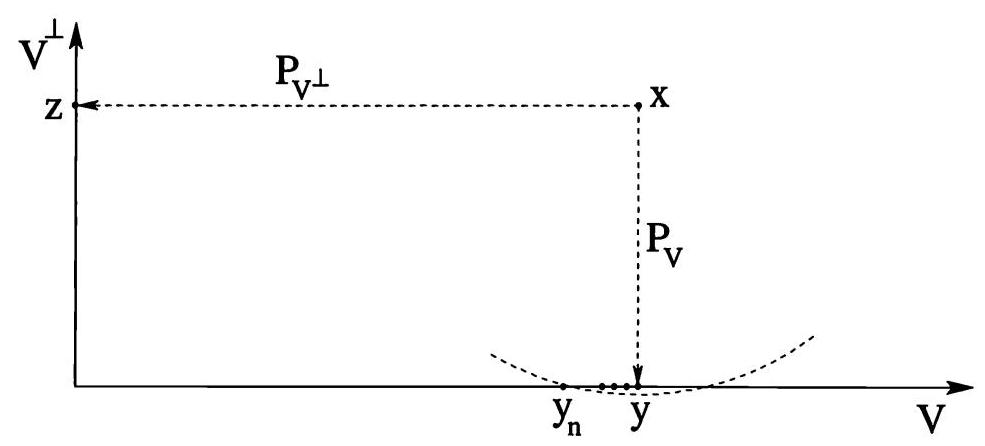
\includegraphics[width=0.9\textwidth]{images/bo_d6ik6nn7aajc739ct1l0_92_246_1195_985_446_0.jpg}
\caption{在子空间 $V$ 及其正交补子空间 ${V}^{ \bot  }$ 上构造正交投影.}
\label{fig:orthogonal-projection}
\end{figure}

\begin{proof}
1. 给定 $x \in  H$ ，我们首先证明存在唯一的点 $y \in  V$ ，其到 $x$ 的距离最小.令
\[
\alpha  \doteq  d\left( {x,V}\right)  \doteq  \mathop{\inf }\limits_{{y \in  V}}\| x - y\| .
\]

则存在点列 ${\left( {y}_{n}\right) }_{n \geq  1}$ ，使得 $\mathop{\lim }\limits_{{n \rightarrow  \infty }}\norm{x - {y}_{n}} = \; \alpha$ .我们断言 ${\left( {y}_{n}\right) }_{n \geq  1}$ 是 Cauchy 列.事实上，对任意两点 $u,v \in  H$ ，有
\[
\| u + v{\| }^{2} + \| u - v{\| }^{2} = 2\| u{\| }^{2} + 2\| v{\| }^{2}.
\]

将此等式应用于 $u = x - {y}_{m}$ 与 $v = x - {y}_{n}$ ，得
\begin{equation}\tag{5.4}\label{eq:projection-cauchy-bound}
{\norm{y}_{m} - {y}_{n}}^{2} = 2{\norm{x} - {y}_{m}}^{2} + 2{\norm{x} - {y}_{n}}^{2} - 4{\norm{x} - \frac{{y}_{m} + {y}_{n}}{2}}^{2}.
\end{equation}

由于 $\frac{{y}_{m} + {y}_{n}}{2} \in  V$ ，故 ${\norm{x} - \frac{{y}_{m} + {y}_{n}}{2}}^{2} \geq  {\alpha }^{2}$ .因此
{\setjot[-2]\begin{align*}
    \mathop{\limsup }\limits_{{m,n \rightarrow  \infty }}{\norm{y}_{m} - {y}_{n}}^{2} &\leq  2\mathop{\limsup }\limits_{{m \rightarrow  \infty }}{\norm{x} - {y}_{m}}^{2} + 2\mathop{\limsup }\limits_{{n \rightarrow  \infty }}{\norm{x} - {y}_{n}}^{2}\\
    &\;\;\;- 4\mathop{\liminf }\limits_{{m,n \rightarrow  \infty }}{\norm{x} - \frac{{y}_{m} + {y}_{n}}{2}}^{2} \\
    &\leq  2{\alpha }^{2} + 2{\alpha }^{2} - 4{\alpha }^{2} = 0
\end{align*}}

证毕.

\noindent 2. 因 $V$ 是闭的(从而完备)，序列 ${\left( {y}_{n}\right) }_{n \geq  1}$ 收敛于唯一极限 $y$ ，且满足 $\| x - y\|  = d\left( {x,V}\right)$.我们断言该点唯一:若对另一点 $\norm{x - {y}^{\prime }} = d\left( {x,V}\right)$ 亦有 ${y}^{\prime }$ ，则同式\eqref{eq:projection-cauchy-bound}中所用论证可得
\[
{\norm{y} - {y}^{\prime }}^{2} = 2{\norm{x} - y}^{2} + 2{\norm{x} - {y}^{\prime }}^{2} - 4{\norm{x} - \frac{y + {y}^{\prime }}{2}}^{2} \leq  2{\alpha }^{2} + 2{\alpha }^{2} - 4{\alpha }^{2},
\]

因为 $\frac{y + {y}^{\prime }}{2} \in  V$ .故 ${y}^{\prime } = y$ .这表明映射 $x \mapsto  {P}_{V}\left( x\right)$ 定义良好.

\noindent 3. 我们现证明 ${P}_{V}\left( x\right)$ 亦可表征为满足下式的唯一一点 $y \in  V$ :
\begin{equation}\tag{5.5}\label{eq:projection-orthogonality}
x - y \in  {V}^{ \bot  }\text{ . }
\end{equation}

任取向量 $v \in  V$ .由步骤 1，对 $\lambda  \in  \mathbb{R}$ ，实值映射
\[
\lambda \; \mapsto  \;{\norm{x} - \left( y + \lambda v\right) }^{2} = {\norm{x} - y}^{2} + {\left| \lambda \right| }^{2}\| v{\| }^{2} + 2\operatorname{Re}\left( {x - y,\;{\lambda v}}\right)
\]

在 $\lambda  = 0$ 处取得其唯一的全局最小值.因此，其在 $\lambda  = 0$ 处的导数必为零.这已证明对每个 $v \in  V$ 均有 $\operatorname{Re}\left( {x - y,v}\right)  = 0$ .若 $H$ 是复Hilbert空间，则可用 $v$ 替换 $- {iv}$，并同样得出 $\operatorname{Im}\left( {x - y,v}\right)  = \operatorname{Re}\left( {x - y, - {iv}}\right)  = 0$ .这就证明了\eqref{eq:projection-orthogonality}.

\noindent 4. 接下来，我们证明满足 $x - y \in  {V}^{ \bot  }$ 的点 $y \in  V$ 是唯一的.事实上，若 ${y}^{\prime } \in  V$ 是另一个满足 $x - {y}^{\prime } \in  {V}^{ \bot  }$ 的点，则
\[
{\norm{y} - {y}^{\prime }}^{2} = \left( {y - {y}^{\prime },y - {y}^{\prime }}\right)  = \left( {y - {y}^{\prime },x - {y}^{\prime }}\right)  - \left( {y - {y}^{\prime },x - y}\right)  = 0
\]

因为 $y - {y}^{\prime } \in  V$ ，而 $x - {y}^{\prime } \in  {V}^{ \bot  }$ 且 $x - y \in  {V}^{ \bot  }$ .

\noindent 5. 最后，我们证明正交投影 ${P}_{V} : H \mapsto  V$ 是一个范数为 $\norm{P}_{V} \leq  1$ 的线性算子.

若 $y = {P}_{V}\left( x\right)$ 且 ${y}^{\prime } = {P}_{V}\left( {x}^{\prime }\right)$ ，则对任意标量 $\alpha ,{\alpha }^{\prime } \in  \mathbb{K}$ ，均有
\[
{\alpha y} + {\alpha }^{\prime }{y}^{\prime } \in  V,\;{\alpha x} + {\alpha }^{\prime }{x}^{\prime } - \left( {{\alpha y} + {\alpha }^{\prime }{y}^{\prime }}\right)  \in  {V}^{ \bot  }.
\]

由第 3 步可知，这足以推出 ${P}_{V}\left( {{\alpha x} + {\alpha }^{\prime }{x}^{\prime }}\right)  = {\alpha y} + {\alpha }^{\prime }{y}^{\prime }$ ，从而证明投影算子 ${P}_{V}$ 是线性的.类似地，算子 ${P}_{{V}^{ \bot  }} = \; I - {P}_{V}$ 也是线性的.

由于向量 ${P}_{V}\left( x\right)$ 与 ${P}_{{V}^{ \bot  }}\left( x\right)  = x - {P}_{V}\left( x\right)$ 正交，根据勾股定理有
\[
{\norm{P}_{V}\left( x\right) }^{2} + {\norm{x} - {P}_{V}\left( x\right) }^{2} = \| x{\| }^{2}.
\]

这证明了 $\norm{P}_{V} \leq  1$ 与 $\norm{P}_{{V}^{ \bot  }} \leq  1$ .
\end{proof}

\begin{remark}\label{rem:projection-norm}
在前述定理中，若 $V \neq  \{ 0\}$ ，则 $\norm{P}_{V} = 1$ ；若 $V \neq  H$ ，则 $\norm{P}_{{V}^{ \bot  }} = 1$ .
\end{remark}

\section{Hilbert空间上的线性泛函}

下一个定理表明，Hilbert空间可与其对偶空间等同.换言之，每个元素 $x \in  H$ 确定一个有界线性泛函 ${\phi }^{x} : H \mapsto  \mathbb{K}$ ，定义为 ${\phi }^{x}\left( y\right)  = \left( {y,x}\right)$ ；反之， $H$ 上的每个有界线性泛函均具有形式 $y \mapsto  \left( {y,x}\right)$ ，其中 $x \in  H$ 为某个元素.

\begin{theorem}[线性泛函的Riesz表示]\label{thm:riesz-representation-functional}
设 $H$ 为一个Hilbert空间.

(i) 对每个 $x \in  H$ ，映射 $y \mapsto  \left( {y,x}\right)$ 是 $H$ 上的一个连续线性泛函.

(ii) 设 $y \mapsto  {Ay}$ 为 $H$ 上的一个连续线性泛函，则存在唯一元素 $\bm{a} \in  H$ ，使得对每个 $y \in  H$ 均有 ${Ay} = \left( {y,\bm{a}}\right)$ .
\end{theorem}

\begin{proof}
(i) 设给定 $x \in  H$ .由内积定义，映射 ${\phi }^{x}$ (定义为 ${\phi }^{x}\left( y\right)  \doteq  \left( {y,x}\right)$ )是线性的.该线性映射的有界性由Cauchy-Schwartz不等式得出:
\[
\norm{\phi }^{x} \doteq  \mathop{\sup }\limits_{{\| y\|  \leq  1}}\left| \left( {y,x}\right) \right|  \leq  \mathop{\sup }\limits_{{\| y\|  \leq  1}}\| y\| \| x\|  = \| x\| .
\]

(ii) 反之，设给定一线性连续泛函 $y \mapsto  {Ay}$ .若对所有 $y \in  H$ 均有 ${Ay} \equiv  0$ ，则结论显然成立，取 $\bm{a} = \bm{0}$ (即 $H$ 中的零向量)即可.

\begin{figure}[htbp]
\centering
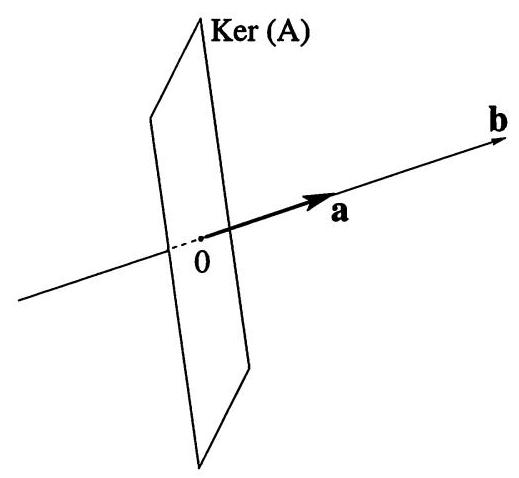
\includegraphics[width=0.4\textwidth]{images/bo_d6ik6nn7aajc739ct1l0_95_483_252_519_478_0.jpg}
\caption{若对每个 $y$ 均有 ${Ay} = \left( {y,\bm{a}}\right)$ ，则向量 a 必与 $\operatorname{Ker}\left( A\right)$ 正交.由于 ${\left(  \operatorname{Ker}\left( A\right) \right)  }^{ \bot  }$ 是一维的，对任意非零向量 $\bm{b} \in  {\left(  \operatorname{Ker}\left( A\right) \right)  }^{ \bot  }$ ，必有 $\bm{a} = t\bm{b}$ ，其中数 $t$ 由恒等式 $A\bm{b} = \left( {\bm{b},t\bm{b}}\right)$ 确定.}
\label{fig:riesz-representation-geometry}
\end{figure}

否则， $V \doteq  \operatorname{Ker}\left( A\right)$ 是一个闭超平面.其正交补 ${V}^{ \bot  }$ 是一个一维子空间.任取一非零向量 $\bm{b} \in  {V}^{ \bot  }$ ，并定义 $\kappa  = A\bm{b}/\| \bm{b}{\| }^{2},\bm{a} \doteq  \overline{\kappa }\bm{b}$ .此选择给出
\begin{equation}\tag{5.6}\label{eq:riesz-key-identity}
0 \neq  A\bm{b} = \kappa \left( {\bm{b},\bm{b}}\right)  = \left( {\bm{b},\overline{\kappa }\bm{b}}\right)  = \left( {\bm{b},\bm{a}}\right) .
\end{equation}

对任意向量 $y \in  H$ ，可将 $y$ 分解为一个属于 $V$ 的向量与属于${V}^{ \bot  }$ 的向量之和:
\[
y = {P}_{V}\left( y\right)  + \alpha \bm{b}
\]

其中 $\alpha  \in  \mathbb{K}$ 为某元素.由\eqref{eq:riesz-key-identity}立即得
\begin{align*}
    {Ay} &= A\left( {{P}_{V}\left( y\right) }\right)  + A\left( {\alpha \bm{b}}\right)  = 0 + {\alpha A}\bm{b} = 0 + \alpha \left( {\bm{b},\bm{a}}\right) \\
    &= \left( {{P}_{V}\left( y\right) ,\bm{a}}\right)  + \left( {\alpha \bm{b},\bm{a}}\right)  = \left( {y,\bm{a}}\right) .
\end{align*}


\end{proof}

\begin{remark}\label{rem:hilbert-dual-identification}
设 $H$ 为实数域上的Hilbert空间.由前述定理，映射 $x \mapsto  {\phi }^{x}$ 是 $H$ 与其对偶空间 ${H}^{ * }$ (即 $H$ 上所有有界线性泛函构成的空间)之间的等距同构.因此，我们可将两个空间 $H$ 与 ${H}^{ * }$ 等同看待.

若此时 $\Lambda  : H \mapsto  H$ 是有界线性算子，则其伴随算子 ${\Lambda }^{ * } : {H}^{ * } \mapsto \; {H}^{ * }$ 可被识别为算子 ${\Lambda }^{ * } : H \mapsto  H$ .该伴随算子由如下恒等式刻画
\[
\left( {x,{\Lambda }^{ * }y}\right)  = \left( {{\Lambda x},y}\right) \;\forall\,x,y \in  H.
\]
\end{remark}

\section{Gram-Schmidt正交化}

设 $H$ 为Hilbert空间.若向量 $x \in  H$ 满足 $\| x\|  = 1$ ，则称其为\bluebf{单位化的}.
\begin{definition}[标准正交]
    设$H$是Hilbert空间，子集 $E \subset  H$ 称为\colorbf{标准正交的}，当且仅当 $E$ 中每个向量的范数均为1，且 $E$ 中任意两个向量彼此正交.
\end{definition}


接下来，考虑有限个线性无关向量构成的集合 $S = \left\{  {{v}_{1},{v}_{2},\ldots ,{v}_{n}}\right\}$ .假设 $x \in  \operatorname{span}\left\{  {{v}_{1},\ldots ,{v}_{n}}\right\}$ ，于是有
\[
x = \sum\limits_{{k = 1}}^{n}{\theta }_{k}{v}_{k}
\]
对某些系数 ${\theta }_{k}$ 成立.为实际计算这些系数，我们注意到:对每个 $j = 1,\ldots ,n$ ，必有
\[
\left( {x,{v}_{j}}\right)  = \sum\limits_{{k = 1}}^{n}{\theta }_{k}\left( {{v}_{k},{v}_{j}}\right) .
\]

因此，数 ${\theta }_{1},\ldots ,{\theta }_{n}$ 可通过求解 $n$ 个线性方程组成的方程组得到
\begin{equation}\tag{5.7}\label{eq:gram-schmidt-linear-system}
\left( \begin{matrix} \left( {{v}_{1},{v}_{1}}\right) & & \left( {{v}_{n},{v}_{1}}\right) \\  \vdots &  \ddots  & \vdots \\  \left( {{v}_{1},{v}_{n}}\right) & \cdots & \left( {{v}_{n},{v}_{n}}\right)  \end{matrix}\right) \left( \begin{matrix} {\theta }_{1} \\  \vdots \\  {\theta }_{n} \end{matrix}\right)  = \left( \begin{matrix} \left( {x,{v}_{1}}\right) \\  \vdots \\  \left( {x,{v}_{n}}\right)  \end{matrix}\right) .
\end{equation}

当矩阵为对角阵(即对所有 $i \neq  j$ 均有 $\left( {{v}_{i},{v}_{j}}\right)  = 0$ )时，该方程组更易求解.这恰好发生在向量 ${v}_{1},{v}_{2},\ldots ,{v}_{n}$ 彼此正交时.此时显式解为
\[
{\theta }_{k} = \frac{\left( x,{v}_{k}\right) }{\left( {v}_{k},{v}_{k}\right) }.
\]

在集合 $\left\{  {{v}_{1},\ldots ,{v}_{n}}\right\}$ 为标准正交的特殊情形下(即对每个 $j = 1,\ldots ,n$ 均有 $\left( {{v}_{j},{v}_{j}}\right)  =$ = 1)，上述公式进一步简化为
\[
{\theta }_{k} = \left( {x,{v}_{k}}\right) .
\]

前述分析表明:若已有标准正交基可用，则计算将变得简便得多.现给定一个(有限或可数的)线性无关集 $S = \left\{  {{v}_{1},{v}_{2},\ldots }\right\}$ ，我们描述一种通用方法，以构造标准正交集 $\left\{  {{e}_{1},{e}_{2},\ldots }\right\}$ ，使得
\[
{E}_{n} \doteq  \operatorname{span}\left\{  {{e}_{1},\ldots ,{e}_{n}}\right\}   = \operatorname{span}\left\{  {{v}_{1},\ldots ,{v}_{n}}\right\}
\]

对每个 $n \geq  1$ 均成立.该构造将通过归纳法实现.

\subsection{Gram-Schmidt正交化算法}

(i) 首先定义 ${e}_{1} \doteq  \frac{{v}_{1}}{\norm{v}_{1}}$ .

(ii) 若已构造出 ${e}_{1},\ldots ,{e}_{n - 1}$ ，令 ${\widetilde{v}}_{n}$ 为 ${v}_{n}$ 在子空间 ${E}_{n - 1} = \operatorname{span}\left\{  {{v}_{1},\ldots ,{v}_{n - 1}}\right\}   = \operatorname{span}\left\{  {{e}_{1},\ldots ,{e}_{n - 1}}\right\}$ 上的垂直投影，然后定义
\begin{equation}\tag{5.8}\label{eq:gram-schmidt-en-def}
{e}_{n} \doteq  \frac{{v}_{n} - {\widetilde{v}}_{n}}{\norm{v}_{n} - {\widetilde{v}}_{n}}.
\end{equation}

注意 ${v}_{n} \neq  {\widetilde{v}}_{n}$ ，因为 ${v}_{n} \notin  \operatorname{span}\left\{  {{v}_{1},\ldots ,{v}_{n - 1}}\right\}$ .故 ${e}_{n}$ 定义良好且范数为1.此外， ${e}_{n}$ 与所有向量 ${e}_{1},\ldots ,{e}_{n - 1}$ 均正交.

注意， ${v}_{n}$ 在子空间 ${E}_{n - 1}$ 上的投影由下式计算:
\[
{\widetilde{v}}_{n} = \sum\limits_{{k = 1}}^{{n - 1}}\left( {{v}_{n},{e}_{k}}\right) {e}_{k}
\]

由式\eqref{eq:gram-schmidt-en-def}，这给出显式公式
\[
{e}_{n} = \frac{{v}_{n} - \sum\limits_{{k = 1}}^{{n - 1}}\left( {{v}_{n},{e}_{k}}\right) {e}_{k}}{\norm{v}_{n} - \sum\limits_{{k = 1}}^{{n - 1}}\left( {v}_{n},{e}_{k}\right) {e}_{k}}.
\]

\begin{figure}[htbp]
\centering
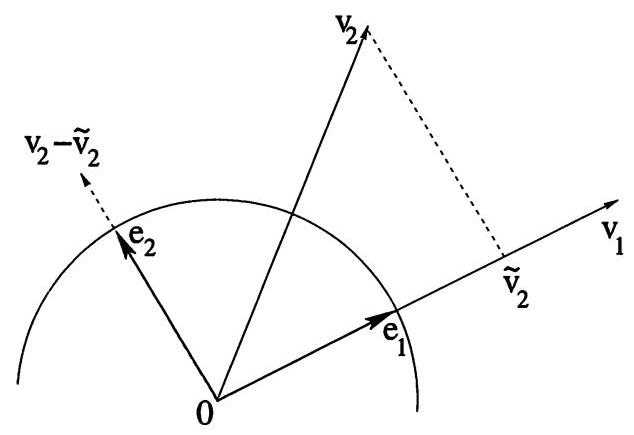
\includegraphics[width=0.6\textwidth]{images/bo_d6ik6nn7aajc739ct1l0_97_408_1210_634_435_0.jpg}
\caption{Gram-Schmidt正交化过程，应用于两个向量 ${v}_{1},{v}_{2}$.}
\label{fig:gram-schmidt-process}
\end{figure}

\section{标准正交集}

若 $\left\{  {{e}_{1},{e}_{2},\ldots ,{e}_{n}}\right\}$ 是 ${\mathbb{R}}^{n}$ 的一组标准正交基，则任意向量 $x \in  {\mathbb{R}}^{n}$ 均可唯一地表示为如下线性组合:
\[
x = \sum\limits_{{k = 1}}^{n}\left( {x,{e}_{k}}\right) {e}_{k}
\]

注意，每一项 $\left( {x,{e}_{k}}\right) {e}_{k}$ 表示向量 $x$ 在由 ${e}_{k}$ 张成的一维子空间上的垂直投影.

在无穷维Hilbert空间 $H$ 中，上述有限和应替换为无穷级数.对许多应用而言，理解该级数在何种条件下收敛、以及何时达到等式至关重要.
\begin{equation}\tag{5.9}\label{eq:orthonormal-expansion}
x = \sum\limits_{{k \geq  1}}\left( {x,{e}_{k}}\right) {e}_{k}
\end{equation}

\begin{lemma}[正交子空间的性质]\label{lem:orthogonal-subspace-properties}
设 $H$ 为一个Hilbert空间.对任意子集 $S \subseteq  H$ ，其正交子空间 ${S}^{ \bot  }$ 是 $H$ 的一个闭子空间.此外，下列命题等价:
\begin{enumerate}[(i)]
    \item $\operatorname{span}\left( S\right)$ 在 $H$ 中稠密.
    \item ${S}^{ \bot  } = \{ 0\}$ .
\end{enumerate}
\end{lemma}

\begin{proof}
1. ${S}^{ \bot  }$ 是 $H$ 的子空间，这一点显然成立.现设 ${x}_{n} \in  {S}^{ \bot  }$ 与 ${x}_{n} \rightarrow  x$ 属于 $n \rightarrow  \infty$ ，则对每个 $a \in  S$ ，有
\[
\left( {x,a}\right)  = \mathop{\lim }\limits_{{n \rightarrow  \infty }}\left( {{x}_{n},a}\right)  = 0.
\]

因此 $x \in  {S}^{ \bot  }$ 亦属其中，表明该子空间是闭的.

\noindent 2. 为证明蕴含关系 (i) $\Rightarrow$ (ii)，假设 $\operatorname{span}\left( S\right)$ 在 $H$ 中稠密，并设 $x \in  {S}^{ \bot  }$ ，因此对每个 $a \in  S$ 均有 $\left( {x,a}\right)  = 0$ .于是存在一列线性组合，记为
\[
{x}_{n} = \sum\limits_{{k = 1}}^{{N}_{n}}{\theta }_{n,k}{a}_{n,k}
\]

其中 ${a}_{n,k} \in  S$ ，且当 $n \rightarrow  \infty$ 时有 ${x}_{n} \rightarrow  x$ .这意味着
{\begin{align*}
    \left( {x,x}\right)  &= \lim_{{n \rightarrow  \infty }}\left( {x,{x}_{n}}\right)  = \lim_{{n \rightarrow  \infty }}\left( {x,\sum_{{k = 1}}^{{N}_{n}}{\theta }_{n,k}{a}_{n,k}}\right)\\
    &=\lim_{n \rightarrow  \infty }\sum_{{k = 1}}^{{N}_{n}}{\theta }_{n,k}\left( {x,{a}_{n,k}}\right)  = 0,
\end{align*}}

从而得出 $x = 0$ .

\noindent 3. 为证明蕴含关系 (ii) $\Rightarrow$ (i)，设 $V$ 为 $\operatorname{span}\left( S\right)$ 的闭包.若 (i) 不成立，则 $V \neq  H$ ，且存在某个元素 $y \notin  V$ .考虑正交投影 ${P}_{V}\left( y\right)$ .于是 $w \doteq  y - {P}_{V}\left( y\right)$ 是一个非零向量，且垂直于 $V$ .由于 $w \in  {S}^{ \bot  }$ ，这与 (ii) 矛盾.
\end{proof}

给定一个标准正交序列，下述定理给出级数\eqref{eq:orthonormal-expansion}的收敛性，并刻画其和.

\begin{theorem}[正交级数的和]\label{thm:orthogonal-series-sum}
设 $S = \left\{  {{e}_{1},{e}_{2},\ldots }\right\}$ 为Hilbert空间 $H$ 中一个(有限或可数的)标准正交集.令 $V$ 为由 $S$ 生成的闭子空间，并记 ${P}_{V} : H \mapsto  V$ 为其垂直投影.则对任意的$x \in  H$ ，均有Bézier不等式
\begin{equation}\tag{5.10}\label{eq:bessel-inequality}
\sum\limits_{{k \geq  1}}{\left| \left( x,{e}_{k}\right) \right| }^{2} = {\norm{P}_{V}x}^{2} \leq  \| x{\| }^{2}.
\end{equation}

此外，
\begin{equation}\tag{5.11}\label{eq:orthogonal-series-sum}
\sum\limits_{{k \geq  1}}\left( {x,{e}_{k}}\right) {e}_{k} = {P}_{V}x
\end{equation}

\end{theorem}

\begin{proof}
1. 对任意 $n \geq  1$ ，记为 ${V}_{n} \doteq  \operatorname{span}\left\{  {{e}_{1},\ldots ,{e}_{n}}\right\}$ .则
\[
{P}_{{V}_{n}}x = \sum\limits_{{k = 1}}^{n}\left( {x,{e}_{k}}\right) {e}_{k}
\]

因此，由标准正交性可得
{\begin{align*}
    {\norm{P}_{{V}_{n}}x}^{2}& = \left( {\sum\limits_{{j = 1}}^{n}\left( {x,{e}_{j}}\right) {e}_{j},\sum\limits_{{k = 1}}^{n}\left( {x,{e}_{k}}\right) {e}_{k}}\right)  = \sum\limits_{{k,j = 1}}^{n}\left( {x,{e}_{j}}\right) \overline{\left( x,{e}_{k}\right) }\left( {{e}_{j},{e}_{k}}\right)\\
    &= \sum\limits_{{k = 1}}^{n}{\left| \left( x,{e}_{k}\right) \right| }^{2}.
\end{align*}}

由于对每个 $n$ 均有 $\norm{{P}_{{V}_{n}}x} \leq  \| x\|$ ，故不等式\eqref{eq:bessel-inequality}得证.

\noindent 2. 若集合 $S$ 有限，则恒等式\eqref{eq:orthogonal-series-sum}显然成立.为涵盖 $S$ 可数的情形，我们首先证明部分和序列
\[
{x}_{n} \doteq  \sum\limits_{{k = 1}}^{n}\left( {x,{e}_{k}}\right) {e}_{k}
\]
是Cauchy列.事实上，级数\eqref{eq:orthogonal-series-sum}中所有项彼此正交.对 $m < n$ ，利用勾股定理及\eqref{eq:bessel-inequality}可得
\[
{\norm{x}_{n} - {x}_{m}}^{2} = \sum\limits_{{k = m + 1}}^{n}{\left| \left( x,{e}_{k}\right) \right| }^{2} \rightarrow  0,\;m,n \rightarrow  \infty .
\]

由于$H$完备，故存在$\widetilde{x}$ ，使得部分和${x}_{n} \rightarrow  \widetilde{x}$ ，即该极限即为级数\eqref{eq:orthogonal-series-sum}之和.

\noindent 3. 为完成证明，需验证 $\widetilde{x} = {P}_{V}x$ .

由于对每个 $n \geq  1$ 和 ${x}_{n} \rightarrow  \widetilde{x}$ 均有 ${x}_{n} \in  V$ ，显然 $\widetilde{x}$ 属于闭子空间 $V$ .此外，
\[
\left( {x - \widetilde{x},{e}_{k}}\right)  = \mathop{\lim }\limits_{{n \rightarrow  \infty }}\left( {x - {x}_{n},{e}_{k}}\right)  = 0
\]

因为一旦 $n \geq  k$ 成立，便有 $\left( {x - {x}_{n},{e}_{k}}\right)  = 0$ .这表明 $x - \widetilde{x}$ 与所有向量 ${e}_{k}$ 均正交，从而亦与这些向量的任意线性组合正交.因此， $x - \widetilde{x}$ 与每个向量 $v \in  V$ 正交.性质 $\widetilde{x} \in  V$ 与 $x - \widetilde{x} \in  {V}^{ \bot  }$ 共同推出 $\widetilde{x} = {P}_{V}x$ .
\end{proof}

\begin{definition}[标准正交基]
    若标准正交集 $S\subset  H$满足$\operatorname{span}\left( S\right)$ 在 $H$ 中稠密，则称$S$为\colorbf{标准正交基}.
\end{definition}
此时，由 $S$ 生成的闭子空间即为 $V = H$ .因而对每个 $x \in  H$ 均有 ${P}_{V}x = x$ ，且由\eqref{eq:bessel-inequality}--\eqref{eq:orthogonal-series-sum}可得
\begin{equation}\tag{5.12}\label{eq:parseval-identity}
\sum\limits_{{k \geq  1}}{\left| \left( x,{e}_{k}\right) \right| }^{2} = \| x{\| }^{2},\;\sum\limits_{{k \geq  1}}\left( {x,{e}_{k}}\right) {e}_{k} = x.
\end{equation}

\subsection{傅里叶级数}
作为前述理论的一个应用，考虑复值函数构成的Hilbert空间 ${L}^{2}\left( {\left(  {-\pi ,\pi }\right)  ;\mathbb{C}}\right)$ ，其内积定义为
\begin{equation}\tag{5.13}\label{eq:L2-inner-product-Fourier}
\left( {f,g}\right)  \doteq  {\int }_{-\pi }^{\pi }f\left( x\right) \overline{g\left( x\right) }{dx}.
\end{equation}

在此空间中，函数集
\[
{\varphi }_{n}\left( x\right)  \doteq  \frac{{e}^{inx}}{\sqrt{2\pi }},\;n \in  \mathbb{Z},
\]
是标准正交的.事实上，
\[
{\int }_{-\pi }^{\pi }{e}^{imx}\overline{{e}^{inx}}{dx} = {\int }_{-\pi }^{\pi }{e}^{i\left( {m - n}\right) x}{dx} = \begin{cases} 0 &m \neq  n, \\  {2\pi } &m = n. \end{cases}
\]

我们断言：
\begin{theorem}[$L^2((-\pi,\pi))$的标准正交基]
    可数集$S \doteq  \left\{  {{e}^{inx};n \in  \mathbb{Z}}\right\}$ 是 ${L}^{2}\left( \left(  {-\pi ,\pi }\right)  \right)$ 的一个标准正交基.
\end{theorem}
\begin{proof}
为证 $S$ 稠密，任取函数 $f \in  {L}^{2}\left( {\left(  {-\pi ,\pi }\right)  ;\mathbb{C}}\right)$ .对任意 $\varepsilon  > 0$ ，存在连续函数 ${f}_{\varepsilon } : \left(  {-\pi ,\pi }\right)   \mapsto  \mathbb{C}$ ，使得
\begin{equation}\tag{5.14}\label{eq:L2-approx-continuous-periodic}
{\norm{f}_{\varepsilon } - f}_{{L}^{2}\left( \left(  {-\pi ,\pi }\right)  \right) } < \varepsilon ,\;{f}_{\varepsilon }\left( {-\pi }\right)  = {f}_{\varepsilon }\left( \pi \right) .
\end{equation}
反之，如第3章例3.8所示，我们可以找到一个如下形式的复三角多项式
\[
p\left( x\right)  = \sum\limits_{{k =  - N}}^{N}{\alpha }_{k}{e}^{ikx}
\]

使得
\begin{equation}\tag{5.15}\label{eq:uniform-trig-approx}
{\norm{f}_{\varepsilon } - p}_{{\mathcal{C}}^{0}\left( \left(  {-\pi ,\pi }\right)  \right) } \doteq  \mathop{\max }\limits_{{x \in  \left(  {-\pi ,\pi }\right)  }}\left| {{f}_{\varepsilon }\left( x\right)  - p\left( x\right) }\right|  < \varepsilon .
\end{equation}

注意到
\[
{\norm{f}_{\varepsilon } - p}_{{L}^{2}} = {\left( {\int }_{-\pi }^{\pi }{\left| {f}_{\varepsilon }\left( x\right)  - p\left( x\right) \right| }^{2}dx\right) }^{1/2} \leq  \sqrt{2\pi }{\norm{f}_{\varepsilon } - p}_{{\mathcal{C}}^{0}},
\]

显然， ${f}_{\varepsilon }$ 也可按 ${L}^{2}$ 范数被三角多项式 $p\left( \cdot \right)$ 逼近.结合\eqref{eq:L2-approx-continuous-periodic}与\eqref{eq:uniform-trig-approx}，我们得出 $\overline{\operatorname{span}\left( S\right) } = {L}^{2}\left( \left(  {-\pi ,\pi }\right)  \right)$ .
\end{proof}



现在考虑复三角级数
\begin{equation}\tag{5.16}\label{eq:complex-fourier-series}
\sum\limits_{{k =  - \infty }}^{\infty }{a}_{k}\frac{{e}^{ikx}}{\sqrt{2\pi }},\;{a}_{k} \doteq  \left( {f,{\varphi }_{k}}\right)  = {\int }_{-\pi }^{\pi }f\left( x\right) \frac{{e}^{-{ikx}}}{\sqrt{2\pi }}{dx}.
\end{equation}

由前述定理可知，该级数在 ${L}^{2}\left( \left(  {-\pi ,\pi }\right)  \right)$ 中收敛于 $f$ ，即
\begin{equation}\tag{5.17}\label{eq:fourier-L2-convergence}
\mathop{\lim }\limits_{{N \rightarrow  \infty }}{\norm{f} - \sum\limits_{{k =  - N}}^{N}{a}_{k}{\varphi }_{k}}_{{L}^{2}\left( \left(  {-\pi ,\pi }\right)  \right) } = 0.
\end{equation}

该结果可重述为
\begin{corollary}\label{cor:fourier-L2-convergence}
设 $f \in  {L}^{2}\left( {\left(  {-\pi ,\pi }\right)  ;\mathbb{C}}\right)$ 是一个复值、平方可和的函数.定义系数
\[
{c}_{k} \doteq  \frac{1}{2\pi }{\int }_{-\pi }^{\pi }f\left( y\right) {e}^{-{iky}}{dy}
\]

则有如下收敛性
\[
\mathop{\lim }\limits_{{N \rightarrow  \infty }}{\int }_{-\pi }^{\pi }{\left| f\left( x\right)  - \sum\limits_{{k =  - N}}^{N}{c}_{k}{e}^{ikx}\right| }^{2}{dx} = 0.
\]
\end{corollary}

\section{正定算子}

线性代数的一个基本问题是求解线性方程组
\[
A\bm{x} = \bm{b},
\]
其中 $A$ 是一个 $n \times  n$ 矩阵， $\bm{b}$ 是 ${\mathbb{R}}^{n}$ 中的一个向量.保证解存在且唯一的条件之一是 $A$ 严格正定.事实上，若内积满足对每个 $x \neq  0$ 均有 $\langle A\bm{x},\bm{x}\rangle  > 0$ ，则 $A$ 必为满秩.因此上述线性方程组存在唯一解.本节将证明，该结论在无穷维Hilbert空间中依然成立.

\begin{definition}\label{def:strictly-positive-definite-operator}
设 $H$ 是一个实数域上的Hilbert空间.称线性算子 $A : H \mapsto  H$ 为严格正定\footnotemark，若存在 $\beta  > 0$ ，使得
\begin{equation}\tag{5.18}\label{eq:strictly-positive-definite}
\left( {{Au},u}\right)  \geq  \beta \| u{\| }^{2}\;\forall\,u \in  H.
\end{equation}
\end{definition}
\footnotetext{{在文献中，满足不等式\eqref{eq:strictly-positive-definite}的算子通常称为严格单调算子.此处我们更倾向称之为严格正定算子，以强调其与线性代数中正定矩阵的联系.}}

\begin{theorem}[正定算子的逆]\label{thm:inverse-positive-definite-operator}
设 $H$ 是一个实Hilbert空间， $A : H \mapsto  H$ 是一个有界线性算子，且严格正定，即满足\eqref{eq:strictly-positive-definite}.则对任意 $f \in  H$ ，存在唯一 $u \doteq  {A}^{-1}f \in  H$ ，使得
\begin{equation}\tag{5.19}\label{eq:positive-definite-inverse-equation}
{Au} = f.
\end{equation}

逆算子 ${A}^{-1}$ 满足
\begin{equation}\tag{5.20}\label{eq:positive-definite-inverse-bound}
\norm{A}^{-1} \leq  \frac{1}{\beta }.
\end{equation}

\end{theorem}

\begin{proof}
在假设\eqref{eq:strictly-positive-definite}下，需证连续映射 $A$ 是单射且满射.

\noindent 1. 由\eqref{eq:strictly-positive-definite}可得
\[
\beta \| u{\| }^{2} \leq  \left( {{Au},u}\right)  \leq  \| {Au}\| \| u\| .
\]

因此
\begin{equation}\tag{5.21}\label{eq:positive-definite-beta-bound}
\beta \| u\|  \leq  \| {Au}\| .
\end{equation}

若 ${Au} = 0$ ，则 $u = 0$ ，从而证得 $\operatorname{Ker}\left( A\right)  = \{ 0\}$ 且 $A$ 是单射.

\noindent 2. 接下来，我们声称 $\operatorname{Range}\left( A\right)$ 是闭映射.考虑任意点列 ${v}_{n} \in  \operatorname{Range}\left( A\right)$ ，满足 ${v}_{n} \rightarrow  v$.需证存在某 $u \in  H$ 使得 $v = {Au}$ .

由假设，存在某 ${u}_{n} \in  H$ 使 ${v}_{n} = A{u}_{n}$ 成立.利用\eqref{eq:positive-definite-beta-bound}可得
\[
\mathop{\limsup }\limits_{{m,n \rightarrow  \infty }}\norm{{u}_{m} - {u}_{n}} \leq  \mathop{\limsup }\limits_{{m,n \rightarrow  \infty }}\frac{1}{\beta }\norm{A{u}_{m} - A{u}_{n}} = \mathop{\limsup }\limits_{{m,n \rightarrow  \infty }}\frac{1}{\beta }\norm{{v}_{m} - {v}_{n}} = 0.
\]

因此序列${\left( {u}_{n}\right) }_{n \geq  1}$ 为Cauchy列，收敛于某个$u \in  H$.由连续性，${Au} = v$ ，证毕.

\noindent 3. 现在我们声称 $\operatorname{Range}\left( A\right)  = H$ .否则，因 $\operatorname{Range}\left( A\right)$ 是闭集，可取非零向量 $w \in  {\left(  \text{ Range }\left( A\right) \right)  }^{ \bot  }$ .但此将导致
\[
\beta \| w{\| }^{2} \leq  \left( {{Aw},w}\right)  = 0,
\]

矛盾.

\noindent 4. 由前述步骤， $A : H \mapsto  H$ 是双射，故方程\eqref{eq:positive-definite-inverse-equation}存在唯一解 $u \doteq  {A}^{-1}f$ .再由\eqref{eq:positive-definite-beta-bound}得
\[
\norm{{A}^{-1}f} = \| u\|  \leq  \frac{\| f\| }{\beta }\;\forall\,f \in  H,
\]

证得\eqref{eq:positive-definite-inverse-bound}.
\end{proof}

前述结果亦可方便地借助双线性型表述.

\begin{theorem}[Lax--Milgram]\label{thm:lax-milgram}
设 $H$ 为实数域上的Hilbert空间， $B : H \times  H \mapsto  \mathbb{R}$ 为连续双线性泛函，即
\begin{gather*}
    B\left(  {{au} + b{u}^{\prime },v}\right)   = {aB}\left(  {u,v}\right)   + {bB}\left(  {{u}^{\prime },v}\right)  ,\\
    B\left(  {u,{av} + b{v}^{\prime }}\right)   = {aB}\left(  {u,v}\right)   + {bB}\left(  {u,{v}^{\prime }}\right)  ,\\
    \left| {B\left(  {u,v}\right)  }\right|  \leq  C\| u\| \| v\| ,
\end{gather*}


对某常数 $C$ 及所有 $u,{u}^{\prime },v,{v}^{\prime } \in  H,a,b \in  \mathbb{R}$ 成立.此外，假设 $B$ 严格正定，即存在常数 $\beta  > 0$ 使得
\[
B\left(  {u,u}\right)   \geq  \beta \| u{\| }^{2}\;\forall\,u \in  H.
\]

则对每个 $f \in  H$ ，存在唯一 $u \in  H$ 满足
\begin{equation}\tag{5.22}\label{eq:lax-milgram-equation}
B\left(  {u,v}\right)   = \left( {f,v}\right) \;\forall\,v \in  H.
\end{equation}

此外，
\begin{equation}\tag{5.23}\label{eq:lax-milgram-solution-bound}
\| u\|  \leq  {\beta }^{-1}\| f\| .
\end{equation}

\end{theorem}

\begin{proof}
对每个固定的 $u \in  H$ ，映射 $v \mapsto  B\left(  {u,v}\right)$ 是 $H$ 上的连续线性泛函.由Riesz表示定理，存在唯一向量，记为 ${Au} \in  H$ ，使得
\[
B\left(  {u,v}\right)   = \left( {{Au},v}\right) \;\forall\,v \in  H.
\]

我们声称 $A$ 是一个有界、正定的线性算子.

$A$ 的线性性易验证.为证 $A$ 有界，注意到对任意 $u \in  H$ ，
\[
\| {Au}\|  \doteq  \mathop{\sup }\limits_{{\| v\|  = 1}}\left| \left( {{Au},v}\right) \right|  = \mathop{\sup }\limits_{{\| v\|  = 1}}\left| {B\left(  {u,v}\right)  }\right|  \leq  C\| u\| .
\]

因此 $\| A\|  \leq  C$ .

此外，
\[
\left( {{Au},u}\right)  \doteq  B\left(  {u,u}\right)   \geq  \beta \| u{\| }^{2},
\]

证明 $A$ 是严格正定的.

现在可应用定理\ref{thm:inverse-positive-definite-operator}，从而得出方程 ${Au} = f$ 存在唯一解 $u = {A}^{-1}f$ ，且满足\eqref{eq:lax-milgram-solution-bound}.根据 $A$ 的定义，这给出了\eqref{eq:lax-milgram-equation}的一个解.
\end{proof}

\section{弱收敛}

\begin{definition}[弱收敛]\label{def:weak-convergence}
设 $H$ 是一个Hilbert空间.称点列 ${x}_{n} \in  H$ 弱收敛于点 $x \in  H$ ，记作 ${x}_{n} \rightharpoonup  x$ ，若
\begin{equation}\tag{5.24}\label{eq:weak-convergence}
\mathop{\lim }\limits_{{n \rightarrow  \infty }}\left( {y,{x}_{n}}\right)  = \left( {y,x}\right), \;\forall\,y \in  H.
\end{equation}
\end{definition}

若弱极限存在，则必唯一.事实上，假设 ${x}_{n} \rightharpoonup  x$ 且 ${x}_{n} \rightharpoonup  \widetilde{x}$ .在 \eqref{eq:weak-convergence} 中取 $y = x - \widetilde{x}$ ，可得
\[
0 = \mathop{\lim }\limits_{{n \rightarrow  \infty }}\left( {x - \widetilde{x},{x}_{n}}\right)  - \mathop{\lim }\limits_{{n \rightarrow  \infty }}\left( {x - \widetilde{x},{x}_{n}}\right)  = \left( {x - \widetilde{x},x}\right)  - \left( {x - \widetilde{x},\widetilde{x}}\right)  = \| x - \widetilde{x}{\| }^{2}.
\]

因此 $x = \widetilde{x}$ .

我们回顾:若 $H$ 是无穷维的，则闭单位球 ${B}_{1} \doteq  \{ x \in  H;\| x\|  \leq  1\}$ (关于范数诱导的拓扑)不是紧集.特别地， ${B}_{1}$ 包含一个标准正交序列 $\left\{  {{e}_{1},{e}_{2},\ldots }\right\}$ ，该序列不具有任何收敛子列.另一方面，若将强收敛替换为弱收敛，则仍可证明一个有用的紧性性质.

\begin{theorem}[弱收敛序列]\label{thm:weak-convergence-sequence}
设 $H$ 是一个Hilbert空间.
\begin{enumerate}[(i)]
    \item 每个弱收敛序列均有界.即，若 ${x}_{n} \rightharpoonup  x$ ，则存在常数 $\norm{x}_{n} \leq  C$ ，使得对所有 $C$ 均有 $n \geq  1$ .
    \item 每个有界点列 ${x}_{n} \in  H$ 均存在一个弱收敛子列: ${x}_{{n}_{j}} \rightharpoonup  x$ (对某个 $x \in  H$ ).
\end{enumerate}
\end{theorem}

\begin{proof}
1. 每个 ${x}_{n}$ 均可视为一个连续线性映射，即从 $H$ 到 $\mathbb{K}$ (实数域或复数域)的映射 $y \mapsto  \left( {y,{x}_{n}}\right)$ . ${x}_{n}$ 的Hilbert范数恰等于其作为 $H$ 上线性泛函的范数，即
\[
\norm{x}_{n} = \mathop{\sup }\limits_{{\| y\|  \leq  1}}\left| \left( {y,{x}_{n}}\right) \right| .
\]

由假设，对每个 $y \in  H$ ，集合 $\left\{  {\left( {y,{x}_{n}}\right) ;n \geq  1}\right\}$ 有界.因此，由第 4 章注记 \noindent 4.2(一致有界性原理)，可数族线性泛函 $\left\{  {{x}_{n};n \geq  1}\right\}$ 一致有界.这就证明了 (i).

\noindent 2. 为证 (ii)，考虑向量空间 $X \doteq  \overline{\operatorname{span}\left\{  {{x}_{n};n \geq  1}\right\}  }$ ，即所有点 ${x}_{1},{x}_{2},\ldots$ 的线性组合所成集合的闭包.我们注意到 $X$ 是可分的.事实上，考虑形如
\[
\sum\limits_{{i = 1}}^{N}{\theta }_{i}{x}_{i}
\]

的有限线性组合全体，其中 $N \geq  1$ 与 ${\theta }_{1},\ldots ,{\theta }_{N}$ 均为有理数.该集合可数，且在 $X$ 中稠密.

由于 $X \subseteq  H$ 本身是Hilbert空间，根据Riesz定理，每个 ${x}_{n}$ 均可被识别为 $X$ 上的有界线性泛函.由第2章定理2.34(Banach-阿劳格鲁定理)，序列 ${\left( {x}_{n}\right) }_{n \geq  1}$ 存在一个弱*收敛子列，记为 ${\left( {x}_{{n}_{j}}\right) }_{j \geq  1}$ .这意味着
\[
\mathop{\lim }\limits_{{j \rightarrow  \infty }}\left( {y,{x}_{{n}_{j}}}\right)  = \varphi \left( y\right) \;\forall\,y \in  X,
\]

对某个有界线性泛函 $\varphi: X \mapsto  \mathbb{K}$ 成立.

\noindent 3. 由Riesz表示定理，存在唯一元素 $x \in  X$ ，使得对所有 $y \in  X$ 均有 $\varphi \left( y\right)  = \left( {y,x}\right)$ .我们通过证明子列 ${x}_{{n}_{j}}$ 在全Hilbert空间 $H$ 中弱收敛于 $x$ 来完成证明.事实上，任取 $y \in  H$ ，记 ${P}_{X} : H \mapsto  X$ 为其正交投影，则有
\[
\mathop{\lim }\limits_{{j \rightarrow  \infty }}\left( {y,{x}_{{n}_{j}}}\right)  = \mathop{\lim }\limits_{{j \rightarrow  \infty }}\left( {{P}_{X}y,{x}_{{n}_{j}}}\right)  = \left( {y,x}\right) .
\]
\end{proof}

本节最后证明:紧算子将弱收敛序列映为强收敛序列.

\begin{theorem}\label{thm:compact-weak-to-strong}
在Hilbert空间 $H$ 中，考虑弱收敛序列 ${x}_{n} \rightharpoonup  x$ .设 $\Lambda  : H \mapsto  H$ 为紧算子，则有强收敛
\begin{equation}\tag{5.25}\label{eq:compact-weak-to-strong}
\norm{\Lambda {x}_{n} - {\Lambda x}} \rightarrow  0.
\end{equation}
\end{theorem}

\begin{proof}
为证\eqref{eq:compact-weak-to-strong}，只需说明:对任意子列 ${\left( {x}_{n}\right) }_{n \in  {I}_{1}}$ ，均可再提取子列 ${\left( {x}_{n}\right) }_{n \in  {I}_{2}}$ (其中 ${I}_{2} \subseteq  {I}_{1}$ )，使得
\[
\mathop{\lim }\limits_{{n \rightarrow  \infty ,n \in  {I}_{2}}}\norm{\Lambda {x}_{n} - {\Lambda x}} = 0.
\]

给定子列 ${\left( {x}_{n}\right) }_{n \in  {I}_{1}}$ .由于该序列弱收敛，由前述定理可知其整体有界，即对每个 $n \in  {I}_{1}$ 均有 $\norm{x}_{n} \leq  C$ .

由于 $\Lambda$ 是紧算子，对此有界序列可再提取子列 ${\left( {x}_{n}\right) }_{n \in  {I}_{2}}$ (其中 ${I}_{2} \subseteq  {I}_{1}$ )，使得其像强收敛:
\[
\mathop{\lim }\limits_{{n \rightarrow  \infty ,n \in  {I}_{2}}}\norm{\Lambda {x}_{n} - y} = 0
\]

对某个 $y \in  H$ 成立.剩余需证 $y = {\Lambda x}$ .

记 ${\Lambda }^{ * }$ 为伴随算子，则有
\[
\left( {v,\Lambda {x}_{n} - {\Lambda x}}\right)  = \left( {{\Lambda }^{ * }v,{x}_{n} - x}\right)  \rightarrow  0\;\forall\,v \in  H,
\]

从而证得弱收敛 $\Lambda {x}_{n} \rightharpoonup  {\Lambda x}$ .由于弱极限唯一，故 ${\Lambda x} = y$ ，证明完成.
\end{proof}

\begin{figure}[htbp]
\centering
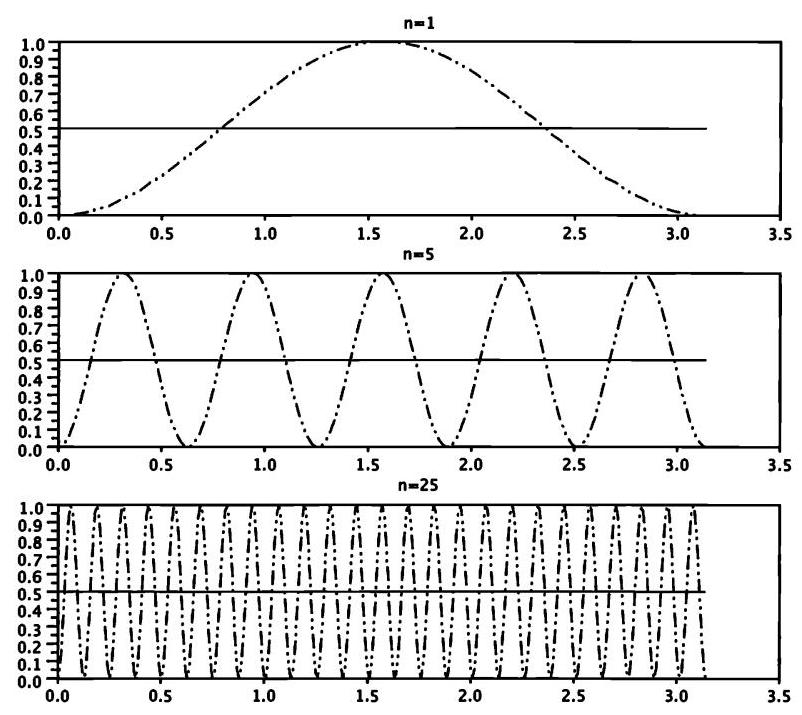
\includegraphics[width=0.7\textwidth]{images/bo_d6ik6nn7aajc739ct1l0_106_338_561_802_715_0.jpg}
\caption{函数 ${f}_{n}\left( x\right)  = {\sin }^{2}{nx}$ 的图像( $n =$ 取1、5、25).当 $n \rightarrow  \infty$ 时，函数 ${f}_{n}$ 既不逐点收敛，也不按 ${L}^{2}$ 范数收敛.然而，我们有弱收敛 ${f}_{n} \rightharpoonup \; f \equiv  1/2$ ，因为 ${f}_{n}$ 在任意区间 $\left(  {a,b}\right)$ 上的平均值均收敛于常数 $1/2$ .}\label{fig:weak-convergence-sin2nx}
\end{figure}

\begin{instance}\label{ins:weak-convergence-sin2nx}
在空间 ${L}^{2}\left( \left(  {0,\pi }\right)  \right)$ 中，考虑函数列 ${f}_{n}\left( x\right)  = {\sin }^{2}{nx}$ (见图\ref{fig:weak-convergence-sin2nx}).我们断言该函数列弱收敛于常值函数 $f\left( x\right)  \equiv  1/2$ .事实上，对任意 $g \in \; {L}^{2}\left( \left(  {0,\pi }\right)  \right)$ ，需证明
\begin{equation}\tag{5.26}\label{eq:weak-sin2nx-mean}
\mathop{\lim }\limits_{{n \rightarrow  \infty }}{\int }_{0}^{\pi }g\left( x\right) {\sin }^{2}\left( nx\right) \,dx = {\int }_{0}^{\pi }\frac{g\left( x\right) }{2}\,dx.
\end{equation}

在如下特殊情形下
\begin{equation}\tag{5.27}\label{eq:step-function-example}
g\left( x\right)  = \begin{cases}
1, & \text{ if }x \in  \left(  {0,b}\right), \\
0, & \text{ if }x \in  \left( b,\pi \right).
\end{cases}
\end{equation}

结论显然成立，因为
\[
\mathop{\lim }\limits_{{n \rightarrow  \infty }}{\int }_{0}^{b}{\sin }^{2}{nxdx} = \mathop{\lim }\limits_{{n \rightarrow  \infty }}\left( {\frac{b}{2} - \frac{\sin {2nb}}{4n}}\right)  = \frac{b}{2} = {\int }_{0}^{\pi }\frac{g\left( x\right) }{2}{dx}.
\]

由线性性可知，\eqref{eq:weak-sin2nx-mean}式对形如\eqref{eq:step-function-example}的函数的所有线性组合——即对所有分段常值函数——均成立.

现考虑任意函数 $g \in  {L}^{2}$ .对任意 $\varepsilon  > 0$ ，可找到一分段常值函数 $\widetilde{g}$ ，使得 $\| g - \widetilde{g}{\| }_{{L}^{2}} < \varepsilon$ .由此可得
\begin{align*}
    &{\int }_{0}^{\pi }g\left( x\right) \left( {{\sin }^{2}{nx} - \frac{1}{2}}\right) {\d x}\\
    &= {\int }_{0}^{\pi }\widetilde{g}\left( x\right) \left( {{\sin }^{2}{nx} - \frac{1}{2}}\right) {\d x} + {\int }_{0}^{\pi }\left(  {\widetilde{g}\left( x\right)  - g\left( x\right) }\right)   \cdot  \left( {{\sin }^{2}{nx} - \frac{1}{2}}\right) {\d x}\\
    &\doteq  {A}_{n} + {B}_{n}.
\end{align*}

由于 $\widetilde{g}$ 是分段常值函数，我们已知当 $n \rightarrow  \infty$ 时， ${A}_{n} \rightarrow  0$ .另一方面，由Cauchy不等式，
\[
\left| {B}_{n}\right|  \leq  \| \widetilde{g} - g{\| }_{{L}^{2}} \cdot  {\left( {\int }_{0}^{\pi }{\left( {\sin }^{2}nx - \frac{1}{2}\right) }^{2}\ d x\right) }^{1/2} < \varepsilon  \cdot  {\left( \frac{\pi }{4}\right) }^{1/2}.
\]

因 $\varepsilon$ 可任取充分小，故证得弱收敛 ${f}_{n} \rightharpoonup  f$ .

注意强收敛并不成立.事实上，
\[
\mathop{\lim }\limits_{{n \rightarrow  \infty }}{\norm{f}_{n} - f}_{{L}^{2}}^{2} = \mathop{\lim }\limits_{{n \rightarrow  \infty }}{\int }_{0}^{\pi }{\left( {\sin }^{2}nx - \frac{1}{2}\right) }^{2}{\d x} = \frac{1}{8}.
\]

接下来，考虑由 ${L}^{2}\left( \left(  {0,\pi }\right)  \right)$ 到其自身的紧算子 $\Lambda$ ，定义为
\[
\left( {\Lambda g}\right) \left( x\right)  \doteq  {\int }_{0}^{x}g\left( y\right) {\d y}.
\]

该积分算子将序列 ${f}_{n}\left( x\right)  = {\sin }^{2}{nx}$ 映为序列
\[
\left( {\Lambda {f}_{n}}\right) \left( x\right)  = {\int }_{0}^{x}{\sin }^{2}{ny\d y} = \frac{x}{2} - \frac{\sin {2nx}}{4n}.
\]

此外， $\left( {\Lambda f}\right) \left( x\right)  = x/2$ .注意到 $\Lambda {f}_{n}$ 在 $\left(  {0,\pi }\right)$ 上一致收敛于 ${\Lambda f}$ .特别地，我们有强收敛 $\| \Lambda {f}_{n} - {\Lambda f}{\| }_{{L}^{2}} \rightarrow  0$ .这为定理\ref{thm:compact-weak-to-strong}提供了例证:紧算子将弱收敛序列映为强收敛序列.
\end{instance}

\section{习题}

\begin{rbhw}[index=1]
设 $H$ 为Hilbert空间.利用内积定义，证明\eqref{eq:inner-product-linearity}中的两个恒等式；并证明勾股定理:若两向量 $x,y \in  H$ 彼此正交，则 $\| x{\| }^{2} + \| y{\| }^{2} = \| x + y{\| }^{2}$ .
\end{rbhw}

\begin{rbhw}
设 $H$ 为具内积 $\left( {\cdot , \cdot  }\right)$ 的向量空间.证明内积是从积空间 $H \times  H$ 到 $\mathbb{K}$ 的连续映射.换言之，若 ${x}_{k} \rightarrow  x$ 且 ${y}_{k} \rightarrow  y$ (按范数\eqref{eq:norm-from-inner-product})，则内积序列 $\left( {{x}_{k},{y}_{k}}\right)$ 收敛于 $\left( {x,y}\right)$.在 $H \times  H$ 上考虑范数 $\| \left( {x,y}\right) \|  \doteq  {\left( \| x{\| }^{2} + \| y{\| }^{2}\right) }^{1/2}$ .
\end{rbhw}

\begin{rbhw}
设 $X$ 为实数域上的Banach空间，其范数为 $\|  \cdot  \|$ .是否存在 $X$ 上的内积 $\left( {\cdot , \cdot  }\right)$ ，使得对每个 $x \in  X$ 均有 $\| x\|  = \sqrt{\left( x,x\right) }$ ？请按以下两个步骤作答.
(i) 设 $H$ 为实Hilbert空间.证明其范数 $\| x\|  = \sqrt{\left( x,x\right) }$ 满足平行四边形恒等式\eqref{eq:parallelogram-identity}
\begin{equation}\tag{5.28}\label{eq:parallelogram-identity}
\| x + y{\| }^{2} + \| x - y{\| }^{2} = 2\| x{\| }^{2} + 2\| y{\| }^{2}\;\forall\,x,y \in  X.
\end{equation}
(ii) 反之，设 $X$ 为实数域上的Banach空间，且其范数满足平行四边形恒等式\eqref{eq:parallelogram-identity}.证明
\[
\left( {x,y}\right)  \doteq  \frac{1}{2}\left( {\| x + y{\| }^{2} - \| x{\| }^{2} - \| y{\| }^{2}}\right)  = \frac{1}{4}\left( {\| x + y{\| }^{2} - \| x - y{\| }^{2}}\right)
\]

是 $X$ 上的一个内积，且恰好给出范数 $\|  \cdot  \|$ .提示:为证明 $\left( {x + {x}^{\prime },y}\right)  = \left( {x,y}\right)  + \left( {{x}^{\prime },y}\right)$ ，首先建立恒等式
\[
{\norm{x} + {x}^{\prime } + y}^{2} = {\norm{x}}^{2} + {\norm{x}^{\prime }}^{2} + \| x + y{\| }^{2} + {\norm{x}^{\prime } + y}^{2} - \frac{1}{2}{\norm{x} + y - {x}^{\prime }}^{2} - \frac{1}{2}{\norm{x}^{\prime } + y - x}^{2}.
\]

为证明 $\left( {{\lambda x},y}\right)  = \lambda \left( {x,y}\right)$ ，先验证该恒等式在 $\lambda$ 为整数时成立，再推广至 $\lambda$ 为有理数的情形，最后由连续性推广至所有 $\lambda  \in  \mathbb{R}$ .
\end{rbhw}

\begin{rbhw}
利用上述问题，证明:

(i) 在向量空间 ${\mathbb{R}}^{2}$ 上，对所有满足 $p \neq  2$ 的 $p \geq  1$ ，范数 $\| \bm{x}{\| }_{p} \doteq  \left( {{\left| {x}_{1}\right| }^{p} + }\right. \; {\left. {\left| {x}_{2}\right| }^{p}\right) }^{1/p}$ 不能由内积生成.

(ii) 在实值连续函数空间 $\mathcal{C}\left( \left(  {0,1}\right)  \right)$ 上，范数 $\| f\|  \doteq \; \mathop{\max }\limits_{{x \in  \left(  {0,1}\right)  }}\left| {f\left( x\right) }\right|$ 不能由内积生成.
\end{rbhw}

\begin{rbhw}
考虑Hilbert空间 $H = {L}^{2}\left( \left(  {-1,1}\right)  \right)$ ，其内积为 $\left( {f,g}\right)  = \; {\int }_{-1}^{1}{fgdx}$ .证明多项式序列 $\left\{  {1,x,{x}^{2},{x}^{3},\ldots }\right\}$ 线性无关，且其张成空间在 $H$ 中稠密.应用Gram-Schmidt正交化过程，构造一组标准正交多项式序列 $\left\{  {{p}_{0},{p}_{1},{p}_{2},{p}_{3},\ldots }\right\}$ (与勒让德多项式成比例).显式计算前三个多项式.
\end{rbhw}

\begin{rbhw}
设 ${\left( {e}_{n}\right) }_{n \geq  1}$ 为Hilbert空间 $H$ 中的一组标准正交序列.证明弱收敛 ${e}_{n} \rightharpoonup  0$ .即证明:对每个 $x \in  H$ ，均有 $\mathop{\lim }\limits_{{n \rightarrow  \infty }}\left( {x,{e}_{n}}\right)  = 0.$
\end{rbhw}

\begin{rbhw}
设 $H$ 为无限维Hilbert空间，给定任意向量 $x \in  H$ ，满足 $\| x\|  \leq  1$ .构造向量序列 ${x}_{n}$ ，使得对每个 $n \geq  1$ 均有 $\norm{x}_{n} = 1$ ，且弱收敛成立: ${x}_{n} \rightharpoonup  x$ .
\end{rbhw}

\begin{rbhw}
设 ${\left( {v}_{k}\right) }_{k \geq  1}$ 为实Hilbert空间 $H$ 中的一列单位向量， ${\left( {\alpha }_{k}\right) }_{k \geq  1}$ 为一列实数.

(i) 若 $\sum\limits_{{k = 1}}^{\infty }\left| {\alpha }_{k}\right|  < \infty$ ，证明级数 $\sum\limits_{{k = 1}}^{\infty }{\alpha }_{k}{v}_{k}$ 收敛.

(ii) 假设序列 ${\left( {v}_{k}\right) }_{k \geq  1}$ 标准正交.此时证明:级数 $\sum\limits_{{k = 1}}^{\infty }{\alpha }_{k}{v}_{k}$ 收敛当且仅当 $\sum\limits_{{k = 1}}^{\infty }{\left| {\alpha }_{k}\right| }^{2} < \infty$ .
\end{rbhw}

\begin{rbhw}
设 $\phi  : {\mathbb{R}}^{n} \mapsto  {\mathbb{R}}^{n}$ 为光滑双射，且雅可比矩阵的行列式对所有 $x \in  {\mathbb{R}}^{n}$ 满足 $\det {D\phi }\left( x\right)  = 1$ ，从而 $\phi$ 保体积.在空间 ${L}^{2}\left( {\mathbb{R}}^{n}\right)$ 上考虑线性算子 $\left( {\Lambda f}\right) \left( x\right)  \doteq  f\left( {\phi \left( x\right) }\right)$ .证明:
\[
\| \Lambda \|  = 1,\;{\Lambda }^{ * } = {\Lambda }^{-1}.
\]

注意， $\Lambda$ 可视为空间 ${L}^{2}\left( {\mathbb{R}}^{n}\right)$ 中的一个旋转，因为其伴随算子等于其逆算子.
\end{rbhw}

\begin{rbhw}
考虑Hilbert空间 ${\ell }^{2}$ ，即所有满足 $\sum\limits_{{k = 1}}^{\infty }{\left| {x}_{k}\right| }^{2} < \infty$ 的实数列 $\bm{x} = \left( {{x}_{1},{x}_{2},\ldots }\right)$ 构成的空间，其内积为 $\left( {\bm{x},\bm{y}}\right)  \doteq  \sum\limits_{{k = 1}}^{\infty }{x}_{k}{y}_{k}$ .定义算子 $\Lambda  : H \mapsto  H$ 如下: $\Lambda \left( {{x}_{1},{x}_{2},{x}_{3},\ldots }\right)  \doteq  \left( {{x}_{2},{x}_{3},{x}_{4},\ldots }\right)$ .计算其伴随算子 ${\Lambda }^{ * }$ .算子 $\Lambda ,{\Lambda }^{ * }$ 是否满射？是否单射？
\end{rbhw}

\begin{rbhw}
设 $S$ 为凸集.称 $x \in  S$ 是 $S$ 的一个极点，若 $x$ 不能表示为 $S$ 中两个不同点的凸组合.换言之，
\[
x \neq  \theta {x}_{1} + \left( {1 - \theta }\right) {x}_{2}\;\text{当}\; 0 < \theta  < 1,\;{x}_{1},{x}_{2} \in  S,\;{x}_{1} \neq  {x}_{2}.
\]

证明以下结论.

(i) 若 $S$ 是Hilbert空间 $H$ 中的闭单位球，则对任意满足 $\| x\|  = 1$ 的点 $x \in  S$ ，它都是 $S$ 的一个极点.特别地，这对空间 $H = {L}^{2}\left( \left(  {0,1}\right)  \right)$ 成立.

(ii) 另一方面，考虑 ${L}^{1}\left( \left(  {0,1}\right)  \right)$ 中的单位球，即
\[
B \doteq  \left\{  {f : \left(  {0,1}\right)   \mapsto  \mathbb{R};{\int }_{0}^{1}\left| {f\left( t\right) }\right| {dt} \leq  1}\right\}  .
\]

证明 $B$ 不包含任何极点.
\end{rbhw}

\begin{rbhw}
设 ${\left( {x}_{n}\right) }_{n > 1}$ 是Hilbert空间 $H$ 中的一列点，满足 $C \doteq \; \mathop{\liminf }\limits_{{n \rightarrow  \infty }}\norm{x}_{n} < \infty$ .证明存在一个弱收敛子列 ${x}_{{n}_{j}} \rightharpoonup  x$ ，其中某点 $x \in  H$ 满足 $\| x\|  \leq  C$ .
\end{rbhw}

\begin{rbhw}
设 $H$ 是一个无限维、可分的实Hilbert空间， ${\ell }^{2}$ 是所有满足 $\| \bm{a}{\| }_{{\ell }^{2}} \doteq \; {\left( \sum\limits_{{k = 1}}^{\infty }{a}_{k}^{2}\right) }^{1/2} < \infty$ 的实数列 $\bm{a} = \left( {{a}_{1},{a}_{2},\ldots }\right)$ 构成的空间.构造一个保距线性双射 $\Lambda  : H \mapsto  {\ell }^{2}$ ，即满足
\[
\| {\Lambda x}{\| }_{{\ell }^{2}} = \| x{\| }_{H}\;\forall\,x \in  H.
\]
\end{rbhw}

\begin{rbhw}
给定实Hilbert空间 $H$ 中的 $n$ 个向量 ${v}_{1},{v}_{2},\ldots ,{v}_{n}$ ，将其Gram行列式定义为\eqref{eq:gram-schmidt-linear-system}式中 $n \times  n$ 阶对称矩阵的行列式:
\[
G\left( {{v}_{1},\ldots ,{v}_{m}}\right)  \doteq  \det \left( \begin{matrix} \left( {{v}_{1},{v}_{1}}\right) & \cdots & \left( {{v}_{n},{v}_{1}}\right) \\  \vdots &  \ddots  & \vdots \\  \left( {{v}_{1},{v}_{n}}\right) & \cdots & \left( {{v}_{n},{v}_{n}}\right)  \end{matrix}\right) .
\]

(i) 利用\eqref{eq:gram-schmidt-linear-system}并取 $x = 0$ ，证明向量 ${v}_{1},\ldots ,{v}_{n}$ 线性无关当且仅当 $G\left( {{v}_{1},\ldots ,{v}_{n}}\right)  \neq  0$ .

(ii) 假设向量 ${v}_{1},\ldots ,{v}_{n}$ 线性无关，考虑子空间 $V \doteq  \operatorname{span}\left\{  {{v}_{1},\ldots ,{v}_{n}}\right\}$ .对任意向量 $x \in  H$ ，证明 $x$ 到 $V$ 的距离为
\[
d\left( {x,V}\right)  = \norm{x - {P}_{V}\left( x\right) } = \sqrt{\frac{G\left( {x,{v}_{1},{v}_{2},\ldots ,{v}_{n}}\right) }{G\left( {{v}_{1},{v}_{2},\ldots ,{v}_{n}}\right) }}.
\]

(iii) 如图\ref{fig:gram-determinant-parallelepiped}所示，证明以 ${v}_{1},\ldots ,{v}_{n}$ 为棱的 $n$ 维平行多面体的体积可表示为
\[
\norm{v}_{1} \cdot  d\left( {{v}_{2};\operatorname{span}\left\{  {v}_{1}\right\}  }\right)  \cdot  d\left( {{v}_{3};\operatorname{span}\left\{  {{v}_{1},{v}_{2}}\right\}  }\right) \cdots d\left( {{v}_{n};\operatorname{span}\left\{  {{v}_{1},\ldots ,{v}_{n - 1}}\right\}  }\right) .
\]

利用 (ii)，证明该平行多面体的体积为 $\sqrt{G\left( {{v}_{1},{v}_{2},\ldots ,{v}_{n}}\right) }$ .

\begin{figure}[htbp]
\centering
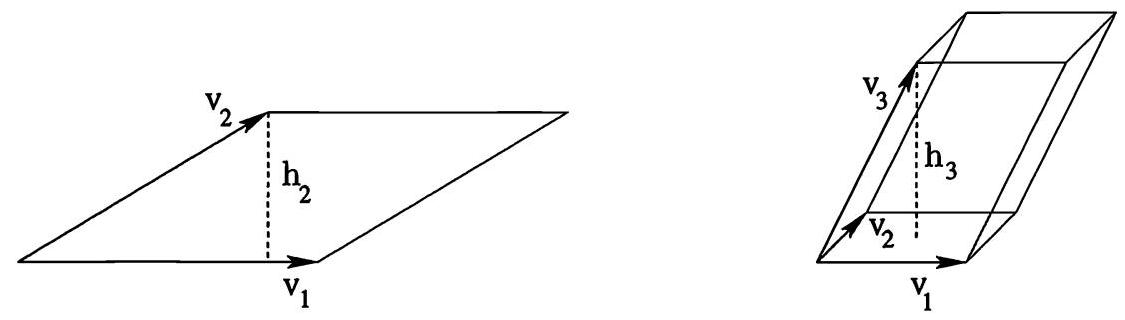
\includegraphics[width=\textwidth]{images/bo_d6ik6nn7aajc739ct1l0_110_169_1151_1125_320_0.jpg}
\caption{计算平行四边形面积与平行多面体体积.此处 ${h}_{2} = d\left( {{v}_{2},\operatorname{span}\left\{  {v}_{1}\right\}  }\right)$ ，而 ${h}_{3} = d\left( {{v}_{3},\operatorname{span}\left\{  {{v}_{1},{v}_{2}}\right\}  }\right) .$}\label{fig:gram-determinant-parallelepiped}
\end{figure}
\end{rbhw}

\begin{rbhw}
设 $f \in  {L}^{2}\left( \mathbb{R}\right)$ .证明存在唯一的偶\footnote{偶函数是指满足 $f(-x) = f(x)$ 的函数}函数 ${g}_{0}$ ，使得
\[
{\norm{f} - {g}_{0}}_{{L}^{2}} = \mathop{\min }\limits_{{g \in  {L}^{2}\left( \mathbb{R}\right) ,g\text{ even }}}\| f - g{\| }_{{L}^{2}}.
\]

显式确定函数 ${g}_{0}$ .
\end{rbhw}

\begin{rbhw}
设 $K \in  \mathcal{B}\left( {X;H}\right)$ 是从 Banach 空间 $X$ 到 Hilbert 空间 $H$ 的有界线性算子.证明下列条件等价.

(i) $K$ 是紧算子.

(ii) 对每个 $\varepsilon  > 0$ ，存在一个具有有限维值域的算子 ${K}_{\varepsilon } : X \mapsto  H$ ，使得 $\norm{{K}_{\varepsilon } - K} < \varepsilon$ .
\end{rbhw}

\begin{rbhw}
设 ${\left\{  {u}_{n}\right\}  }_{n \geq  1}$ 和 ${\left\{  {v}_{n}\right\}  }_{n \geq  1}$ 是 Hilbert 空间 $H$ 中的两个标准正交集.假设
\[
\sum\limits_{{n = 1}}^{\infty }\norm{{u}_{n} - {v}_{n}} < 1
\]

证明:若其中一个集合是完备的，则另一个集合也完备.
\end{rbhw}

\begin{rbhw}
设 $\left\{  {{u}_{n};n \geq  1}\right\}$ 是 Hilbert 空间 $H$ 中一组可数的线性无关单位向量.考虑向量 $v \doteq  \sum\limits_{{n = 1}}^{\infty }{2}^{-n}{u}_{n}$ .

(i) 假设所有向量 ${u}_{n}$ 两两正交，证明集合 $S \doteq  \left\{  {v,{u}_{1},{u}_{2},{u}_{3},\ldots }\right\}$ 线性无关.

(ii) 举一反例说明:若向量 ${u}_{n}$ 并非两两正交，则上述集合 $S$ 可能线性相关.
\end{rbhw}

\begin{rbhw}
给定 Hilbert 空间 $H$ 中的序列 ${\left( {x}_{n}\right) }_{n \geq  1}$ ，证明强收敛 $\norm{{x}_{n} - x} \rightarrow  0$ 成立当且仅当
\[
\norm{x}_{n} \rightarrow  \| x\| \;\text{ and }\;{x}_{n} \rightharpoonup  x\text{ (弱收敛). }
\]
\end{rbhw}

\begin{rbhw}
设 $Q = \left(  {0,1}\right)   \times  \left(  {0,1}\right)$ 为单位正方形.在空间 ${L}^{2}\left( Q\right)$ 中，考虑仅依赖于变量 $y$ 的所有函数构成的子空间:
\[
U = \left\{  {u \in  {L}^{2}\left( Q\right) ;\exists\,\varphi  : \left(  {0,1}\right)   \mapsto  \mathbb{R},u\left( {x,y}\right)  = \varphi \left( y\right)},\,\text{a.e.}\,{\left( {x,y}\right)  \in  Q}\right\}  \text{ . }
\]
(i) 求正交补子空间 $W = {U}^{ \bot  }$ .

(ii) 对任意 $f \in  {L}^{2}\left( Q\right)$ ，确定函数 $g \in  U$ ，使得
\[
\| f - g{\| }_{{L}^{2}\left( Q\right) } = \mathop{\min }\limits_{{u \in  U}}\| f - u{\| }_{{L}^{2}\left( Q\right) }.
\]
\end{rbhw}

\begin{rbhw}
设 $H$ 是 Hilbert 空间， $\Omega  \subset  H$ 是其闭凸子集.

(i) 证明:对任意 $x \in  H$ ，存在唯一一点 $y \in  \Omega$ ，使得 $\| y - x\|  = \mathop{\min }\limits_{{\omega  \in  \Omega }}\| \omega  - x\|$ .该最小距离点 $y = {\pi }_{\Omega }\left( x\right)$ 称为 $x$ 到 $\Omega$ 的垂足投影.

(ii) 证明: $y = {\pi }_{\Omega }\left( x\right)$ 当且仅当 $\langle \omega  - y,y - x) \geq  0$ 对所有 $\omega  \in  \Omega$ 成立.
\end{rbhw}

\begin{rbhw}
在Hilbert空间 $H = {L}^{2}\left( \mathbb{R}\right)$ 上，考虑子集
\[
\Omega  \doteq  \left\{  {f;f\left( x\right)  \leq  {e}^{x}\text{ for a.e. }x \in  \mathbb{R}}\right\}  .
\]

(i) 证明 $\Omega$ 是 $H$ 的闭凸子集.

(ii) 证明到 $\pi  : H \mapsto  \Omega$ 的正交投影即为定义为 $\left( {\pi f}\right) \left( x\right)  = \min \left\{  {f\left( x\right) ,{e}^{x}}\right\}  .$ 的映射.
\end{rbhw}

\begin{rbhw}
在Hilbert空间 $H = {L}^{2}\left( \mathbb{R}\right)$ 上，考虑由 $\left( {\Lambda f}\right) \left( x\right)  = f\left( \left| x\right| \right)$ 定义的线性算子 $\Lambda  : H \mapsto  H$ .

(i) 求 $\Lambda$ 的算子范数.

(ii) 求 $\Lambda$ 的核与值域.

(iii) 计算 ${\Lambda }^{ * }$ 的伴随算子.
\end{rbhw}

\begin{rbhw}
在Hilbert空间 $H = {L}^{2}\left( \left(  {0,\infty }\right)  \right)$ 上，考虑线性算子 $\left( {\Lambda f}\right) \left( x\right)  = f\left( {e}^{x}\right)$ .

(i) 计算线性算子 $\Lambda$ 的范数.

(ii) 求 $\Lambda$ 的核与值域.

(iii) 计算 ${\Lambda }^{ * }$ 的伴随算子.
\end{rbhw}

\begin{rbhw}
考虑函数列 ${f}_{n} \in  {L}^{2}\left( \left(  {0,T}\right)  \right)$ 的有界性.当 $n \rightarrow  \infty$ 时，证明弱收敛 ${f}_{n} \rightharpoonup  f$ 成立当且仅当
\[
\mathop{\lim }\limits_{{n \rightarrow  \infty }}{\int }_{0}^{b}{f}_{n}\left( x\right) {dx} = {\int }_{0}^{b}f\left( x\right) {dx}\;\text{ for every }b \in  \left(  {0,T}\right)  .
\]
\end{rbhw}

\begin{rbhw}
在空间 ${L}^{2}\left( \left(  {0,1}\right)  \right)$ 上，考虑如下两列函数
\[
{f}_{n}\left( x\right)  = \sqrt{n} \cdot  \cos {nx},\;{f}_{n}\left( x\right)  = \left\{  \begin{matrix} {n}^{2/3} & \text{ if } & x \in  \left(  {0,{n}^{-1}}\right)  , \\  0 & \text{ if } & x > {n}^{-1}. \end{matrix}\right.
\]

(i) 两种情形下，均证明对每个 $b \in  \left(  {0,1}\right)$ 有 $\mathop{\lim }\limits_{{n \rightarrow  \infty }}{\int }_{0}^{b}{f}_{n}\left( x\right) {dx} = 0$ .

(ii) 通过取线性组合，证明对每个分段常值函数 $g$ 有 $\mathop{\lim }\limits_{{n \rightarrow  \infty }}{\int }_{0}^{1}{f}_{n}{gdx} = 0$ .

(iii) 是否成立 ${f}_{n} \rightharpoonup  0$ ？
\end{rbhw}

\begin{rbhw}
设 ${\left( {x}_{n}\right) }_{n \geq  1}$ 是Hilbert空间 $H$ 中的一个序列，证明下列命题等价.

(i) 弱收敛成立: ${x}_{n} \rightharpoonup  x$ .

(ii) 序列 $\left( {x}_{n}\right)$ 有界，且对某个具有非空内部闭包的子集 $S \subseteq  H$ 中的所有 $y$ 均有 $\left( {y,{x}_{n}}\right)  \rightarrow  \left( {y,x}\right)$ .
\end{rbhw}

\begin{rbhw}
设 $\Omega  \subseteq  {\mathbb{R}}^{N}$ 为开集.证明函数列 ${f}_{n} \in  {L}^{2}\left( \Omega \right)$ 弱收敛于 $f$ 当且仅当存在常数 $C$ ，使得对每个 $n \geq  1$ 均有 ${\norm{f}_{n}}_{{L}^{2}} \leq  C$ ，且此外
\[
\mathop{\lim }\limits_{{n \rightarrow  \infty }}{\int }_{Q}{f}_{n}{dx} = {\int }_{Q}{fdx}
\]

对每个完全包含于 $\Omega$ 中的矩形 $Q = \left(  {{a}_{1},{b}_{1}}\right)   \times  \left(  {{a}_{2},{b}_{2}}\right)   \times  \cdots  \times  \left(  {{a}_{N},{b}_{N}}\right)$ 均成立.
\end{rbhw}

\begin{rbhw}
在实Hilbert空间 $H$ 中，考虑弱收敛序列: ${x}_{n} \rightharpoonup  y$ .令 $S \doteq  \overline{\operatorname{co}\left\{  {{x}_{n};n \geq  1}\right\}  }$ 为包含所有点 ${x}_{n}$ 的最小闭凸集.证明 $y \in  S$ .
\end{rbhw}

\chapter{Hilbert空间上的紧算子}\vspace{-2em}

对于有限维空间中的线性算子 $A : {\mathbb{R}}^{n} \mapsto  {\mathbb{R}}^{n}$ ，其核、值域、特征值与特征向量等方面已有若干结论.特别地:

(i) $A$ 是单射当且仅当 $A$ 是满射.事实上，子空间 $\operatorname{Ker}\left( A\right)$ 与 ${\left(  \operatorname{Range}\left( A\right) \right)  }^{ \bot  }$ 具有相同维数.

(ii) 若 $A$ 是对称的，则其特征值为实数；此外，空间 ${\mathbb{R}}^{n}$ 存在一组由 $A$ 的特征向量构成的标准正交基.

本章中，我们将证明类似结论，其适用于Hilbert空间 $H$ 上的无穷维算子 $\Lambda$ .事实上，(i) 对形如 $\Lambda  = I - K$ 的算子仍成立，其中 $I$ 是恒等算子， $K$ 是紧算子；此外，(ii) 中的命题可推广至任意紧自伴算子 $\Lambda  : H \mapsto  H$ .

\section{Fredholm理论}

设 $H$ 是一个Hilbert空间.我们回顾:有界线性算子 $K$ : $H \mapsto  H$ 是紧的，若对任意有界点列 ${u}_{n} \in  H$ ，均可提取子列 ${\left( {u}_{{n}_{j}}\right) }_{j \geq  1}$ ，使得像收敛: $K{u}_{{n}_{j}} \rightarrow  v$ (对某个 $v \in  H$ ).

下一个定理描述了形如 $I - K$ 的算子及其伴随算子的核与值域之间的若干关系.

\begin{theorem}[Fredholm]\label{thm:fredholm}
设 $H$ 是实数域上的Hilbert空间， $K : H \mapsto  H$ 是紧线性算子，则

(i) $\operatorname{Ker}\left( {I - K}\right)$ 是有限维的；

(ii) $\operatorname{Range}\left( {I - K}\right)$ 是闭的；

(iii) $\operatorname{Range}\left( {I - K}\right)  = \operatorname{Ker}{\left( I - {K}^{ * }\right) }^{ \bot  }$ ；

(iv) $\operatorname{Ker}\left( {I - K}\right)  = \{ 0\}$ 当且仅当 $\operatorname{Range}\left( {I - K}\right)  = H$ ；

(v) $\operatorname{Ker}\left( {I - K}\right)$ 与 $\operatorname{Ker}\left( {I - {K}^{ * }}\right)$ 具有相同维数.
\end{theorem}

\begin{proof}
1. 若 $\left( {I - K}\right)$ 的核是无穷维的，则可在 $\operatorname{Ker}\left( {I - K}\right)$ 中找到一列标准正交序列 ${\left( {e}_{n}\right) }_{n \geq  1}$ .此时对每个 $n$ 有 $K{e}_{n} = {e}_{n}$ ；此外，由勾股定理，对 $m \neq  n$ 有
\[
\norm{e_m-e_n}^{2} = \norm{e_m}^{2} + \norm{e_n}^{2} = 2
\]

因此对每个 $m \neq  n$ 有 $\norm{K{e}_{m} - K{e}_{n}} = \norm{{e}_{m} - {e}_{n}} = \sqrt{2}$ .故从序列 ${\left( K{e}_{n}\right) }_{n \geq  1}$ 中无法提取任何收敛子列.这一矛盾确立了 (i).

\noindent 2. 为证 (ii)，我们首先证明存在 $\beta  > 0$ ，使得
\begin{equation}\tag{6.1}\label{eq:fredholm-estimate}
\| u - {Ku}\|  \geq  \beta \| u\|,\;\forall\,u \in  \operatorname{Ker}{\left( I - K\right) }^{ \bot  }.
\end{equation}

事实上，若\eqref{eq:fredholm-estimate}不成立，则可找到点列 ${u}_{n} \in  \operatorname{Ker}{\left( I - K\right) }^{ \bot  }$ ，使得 $\norm{u}_{n} = 1$ 且 $\norm{{u}_{n} - K{u}_{n}} < 1/n$ .

由于序列 ${\left( {u}_{n}\right) }_{n \geq  1}$ 有界，通过提取子列并重新标号，可设该序列弱收敛，即 ${u}_{n} \rightharpoonup  u$ (对某个 $u \in  H$ ).

由于 $K$ 是紧算子，由定理\ref{thm:compact-weak-to-strong}可知这蕴含强收敛 $K{u}_{n} \rightarrow  {Ku}$ .我们现得到
\[
\norm{{u}_{n} - {Ku}}\; \leq  \;\norm{{u}_{n} - K{u}_{n}} + \norm{K{u}_{n} - {Ku}}\; \rightarrow  ,\;0\;\text{ 当 }\,n \rightarrow  \infty .
\]
这给出强收敛 ${u}_{n} \rightarrow  {Ku}$ .结合弱收敛 ${u}_{n} \rightharpoonup  u$ ，可知 $u = {Ku}$ 与 ${u}_{n} \rightarrow  u$ 均强收敛.

由构造可知，我们现已有
\[
\| u\|  = \mathop{\lim }\limits_{{n \rightarrow  \infty }}\norm{u}_{n} = 1,\;u \in  \operatorname{Ker}{\left( I - K\right) }^{ \bot  },
\]

但同时， $u - {Ku} = 0$ ，故 $u \in  \operatorname{Ker}\left( {I - K}\right)$ .因此我们得出矛盾，从而证得\eqref{eq:fredholm-estimate}.

\noindent 3. 我们现证明 Range $\left( {I - K}\right)$ 是闭的.考虑点列 ${v}_{n} \in  \operatorname{Range}\left( {I - K}\right)$ ，其中 ${v}_{n} \rightarrow  v$ 当 $n \rightarrow  \infty$ .我们需要找到某个 $u$ ，使得 $v = u - {Ku}$ .由假设，对每个 $n \geq  1$ ，存在 ${u}_{n}$ 满足 ${v}_{n} = {u}_{n} - K{u}_{n}$ .注意，若对某个 $u \in  H$ 有 ${u}_{n} \rightarrow  u$ ，则由连续性可立即推出 $v = u - {Ku}$ .但一般而言，无法保证序列 ${\left( {u}_{n}\right) }_{n \geq  1}$ 收敛.

为克服这一困难，令 ${\widetilde{u}}_{n}$ 为 ${u}_{n}$ 在 $\operatorname{Ker}\left( {I - K}\right)$ 上的正交投影，并令 ${z}_{n} \doteq  {u}_{n} - {\widetilde{u}}_{n}$.这些定义导出
\[
{z}_{n}\; \doteq  \;{u}_{n} - {\widetilde{u}}_{n}\; \in  \mathrm{{Ker}}{\left( I - K\right) }^{ \bot  },\;{v}_{n}\; = \;{u}_{n} - K{u}_{n}\; = \;{z}_{n} - K{z}_{n}\;.
\]

利用\eqref{eq:fredholm-estimate}，对任意指标对 $m,n$ ，我们得到
\[
\norm{{v}_{m} - {v}_{n}} \geq  \beta \norm{{z}_{m} - {z}_{n}}.
\]

由于序列 ${\left( {v}_{n}\right) }_{n \geq  1}$ 是 Cauchy 列，这表明序列 ${\left( {z}_{n}\right) }_{n \geq  1}$ 也是 Cauchy 列.因此存在 $u \in  H$ ，使得 ${z}_{n} \rightarrow  u$ ，从而有
\[
u - {Ku} = \mathop{\lim }\limits_{{n \rightarrow  \infty }}{z}_{n} - K{z}_{n} = \mathop{\lim }\limits_{{n \rightarrow  \infty }}{v}_{n} = v
\]

\begin{figure}[htbp]
\centering
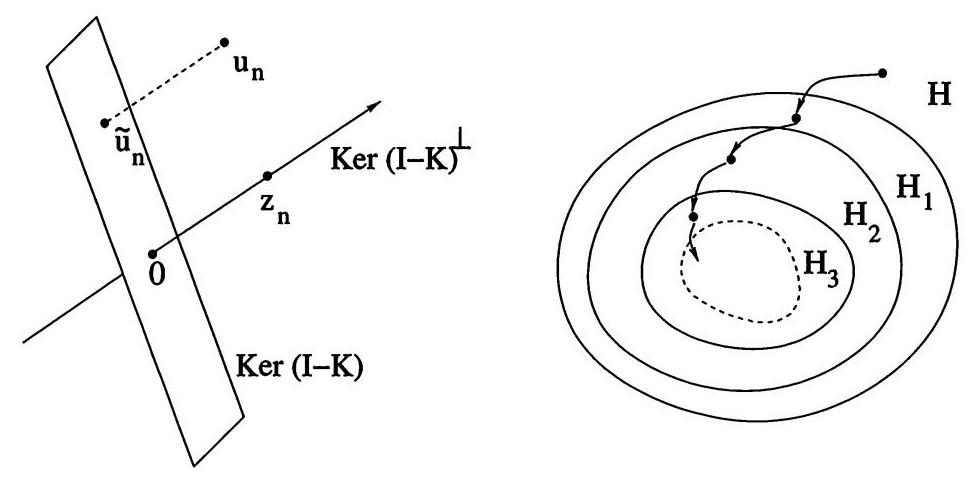
\includegraphics[width=0.9\textwidth]{images/bo_d6ik6nn7aajc739ct1l0_115_253_988_972_477_0.jpg}
\caption{左:通过选取 ${z}_{n} \in  \operatorname{Ker}{\left( I - K\right) }^{ \bot  }$ ，我们实现不等式 $\beta \norm{z}_{n} \leq  \norm{v}_{n}$ ，该式在 (ii) 的证明中使用.右:若 $I - K$ 是单射但不满射，则子空间列 ${H}_{n} \doteq \; {\left( I - K\right) }^{n}\left( H\right)$ 严格递减.这导致矛盾，用于 (iv) 的证明.}
\label{fig:fredholm-proof-geometry}
\end{figure}

\noindent 4. 由于 Range $\left( {I - K}\right)$ 与 $\operatorname{Ker}{\left( I - {K}^{ * }\right) }^{ \bot  }$ 均为闭子空间，断言 (iii) 成立当且仅当
\begin{equation}\tag{6.2}\label{eq:fredholm-range-orth-ker-adjoint}
\operatorname{Range}{\left( I - K\right) }^{ \bot  } = \operatorname{Ker}\left( {I - {K}^{ * }}\right) .
\end{equation}

这可通过观察以下命题彼此等价而得证:
{\setjot[-3]\begin{align*}
    x &\in  \operatorname{Ker}\left( {I - {K}^{ * }}\right) , \\
    \left( {I - {K}^{ * }}\right) x &= 0, \\
    \left( {y,\left( {I - {K}^{ * }}\right) x}\right)  &= 0,\;\forall\,\;y \in  H, \\
    \left( {\left( {I - K}\right) y,x}\right)  &= 0,\;\forall\,\;y \in  H, \\
    x &\in  \operatorname{Range}{\left( I - K\right) }^{ \bot  }.
\end{align*}}


\noindent 5. 为证明 (iv)，假设 $\operatorname{Ker}\left( {I - K}\right)  = \{ 0\}$ ，即算子 $I - K$ 是单射.若 $\operatorname{Range}\left( {I - K}\right)  \neq  H$，我们将导出矛盾.

事实上，假设该值域并非整个空间: ${H}_{1} \doteq  (I - \; K)\left( H\right)  \neq  H$ .由(ii)可知， ${H}_{1}$ 是 $H$ 的一个闭子空间.由于 $I - K$ 是单射，必有
\[
{H}_{2} \doteq  \left( {I - K}\right) \left( {H}_{1}\right)  \subset  {H}_{1}.
\]

我们可通过归纳法继续此过程:对每个 $n$ ，定义
\[
{H}_{n} \doteq  {\left( I - K\right) }^{n}\left( H\right) .
\]

由归纳法可知，每个 ${H}_{n}$ 均为 $H$ 的闭子空间，且
\[
H \supset  {H}_{1} \supset  {H}_{2} \supset  \cdots
\]

对每个 $n \geq  1$ ，现取向量 ${e}_{n} \in  {H}_{n} \cap  {H}_{n + 1}^{ \bot  }$ 使得 $\norm{e}_{n} = 1$ .注意，若 $m < n$ ，则
\[
K{e}_{m} - K{e}_{n} =  - \left( {{e}_{m} - K{e}_{m}}\right)  + \left( {{e}_{n} - K{e}_{n}}\right)  + \left( {{e}_{m} - {e}_{n}}\right)  = {e}_{m} + {z}_{m}
\]

其中 ${z}_{m} \doteq   - \left( {{e}_{m} - K{e}_{m}}\right)  + \left( {{e}_{n} - K{e}_{n}}\right)  - {e}_{n} \in  {H}_{m + 1}$ .

由于 ${e}_{m} \in  {H}_{m + 1}^{ \bot  }$ ，由勾股定理可知
\[
\norm{K{e}_{m} - K{e}_{n}} \geq  \norm{e}_{m} = 1
\]

因此，序列 ${\left( K{e}_{n}\right) }_{n \geq  1}$ 不可能有任何强收敛子列，与 $K$ 的紧性矛盾.

\noindent 6. 为证明(iv)的逆命题，我们采用对偶性论证.假设 $\operatorname{Range}\left( {I - K}\right)  = H$ .由定理\ref{thm:adjoint-properties}，
\[
\operatorname{Ker}\left( {I - {K}^{ * }}\right)  = \operatorname{Range}{\left( I - K\right) }^{ \bot  } = {H}^{ \bot  } = \{ 0\} .
\]
由于 ${K}^{ * }$ 是紧算子，由前一步可知 $\operatorname{Range}\left( {I - {K}^{ * }}\right)  = H$ .再次应用定理\ref{thm:adjoint-properties}，即得 $\operatorname{Ker}\left( {I - K}\right)  = \operatorname{Range}{\left( I - {K}^{ * }\right) }^{ \bot  } = {H}^{ \bot  } = \{ 0\}$ ，结论成立.

\noindent 7. 为证明(v)，我们首先说明 $\operatorname{Ker}\left( {I - K}\right)$ 的维数不小于 Range ${\left( I - K\right) }^{ \bot  }$ 的维数.事实上，反设
\begin{equation}\tag{6.3}\label{eq:fredholm-dim-inequality}
\dim \operatorname{Ker}\left( {I - K}\right)  < \dim \operatorname{Range}{\left( I - K\right) }^{ \bot  }.
\end{equation}

则存在一个线性映射 $A : \operatorname{Ker}\left( {I - K}\right)  \mapsto  \operatorname{Range}{\left( I - K\right) }^{ \bot  }$ ，其为单射但非满射.我们将 $A$ 扩展为定义在整个空间 $H$ 上的线性映射 $A : H \mapsto$ :Range ${\left( I - K\right) }^{ \bot  }$ ，要求当 $u \in  \operatorname{Ker}{\left( I - K\right) }^{ \bot  }$ 时 ${Au} = 0$ .由于 $A$ 的值域是有限维的，故算子 $A$ 是紧的，从而 $K + A$ 也是紧的.

我们声称 $\operatorname{Ker}\left( {I - \left( {K + A}\right) }\right)  = \{ 0\}$ .事实上，任取向量 $u \in  H$ 并将其写为
\[
u = {u}_{1} + {u}_{2},\;{u}_{1} \in  \operatorname{Ker}\left( {I - K}\right) ,\;{u}_{2} \in  \operatorname{Ker}{\left( I - K\right) }^{ \bot  }.
\]

由此得到
\begin{equation}\tag{6.4}\label{eq:fredholm-direct-sum-decomposition}
\left( {I - K - A}\right) \left( {{u}_{1} + {u}_{2}}\right) 
= \left( {I - K}\right) {u}_{2} - A{u}_{1}
\in  \operatorname{Range}\left( {I - K}\right)  \oplus  \operatorname{Range}{\left( I - K\right) }^{ \bot  }.
\end{equation}

由于 $\left( {I - K}\right) {u}_{2}$ 与 $A{u}_{1}$ 正交，和式 $\left( {I - K}\right) {u}_{2} + A{u}_{1}$ 仅当 $\left( {I - K}\right) {u}_{2} = 0$ 且 $A{u}_{1} = 0$ 时才能为零.回顾算子 $I - K$ 在 $\operatorname{Ker}{\left( I - K\right) }^{ \bot  }$ 上是一对一的，且 $A$ 在 $\operatorname{Ker}\left( {I - K}\right)$ 上是一对一的，我们得出 ${u}_{1} = {u}_{2} = 0$ .

将(iv)应用于紧算子 $K + A$ ，得到值域 $(I - \; \left( {K + A}\right) ) = H$ .然而这是不可能的:由构造可知，存在一个向量 $v \in  \operatorname{Range}{\left( I - K\right) }^{ \bot  }$ 满足 $v \notin  \operatorname{Range}\left( A\right)$ .根据\eqref{eq:fredholm-direct-sum-decomposition}，方程
\[
u - {Ku} - {Au} = v
\]

无解.这一矛盾表明\eqref{eq:fredholm-dim-inequality}不可能成立.

\noindent 8. 回顾值域 ${\left( I - {K}^{ * }\right) }^{ \bot  } = \operatorname{Ker}\left( {I - K}\right)$ ，由前一步可推出
\[
\dim \operatorname{Ker}\left( {I - {K}^{ * }}\right)  \geq  \dim \operatorname{Range}{\left( I - {K}^{ * }\right) }^{ \bot  } = \dim \operatorname{Ker}\left( {I - K}\right) .
\]

交换 $K$ 与 ${K}^{ * }$ 的角色，可得相反的不等式.
\end{proof}

\begin{note}[Fredholm择一性]\label{rem:fredholm-alternative}
当 $K$ 为紧算子时，上述定理提供了关于线性方程
\begin{equation}\tag{6.5}\label{eq:fredholm-equation}
u - {Ku} = f.
\end{equation}

解的存在性与唯一性的信息.具体而言，可能出现两种情形.

情形1: $\operatorname{Ker}\left( {I - K}\right)  = \{ 0\}$ .此时算子 $I - K$ 是一对一且满射的.对任意 $f \in  H$ ，方程\eqref{eq:fredholm-equation}恰有唯一解.

情形2: $\operatorname{Ker}\left( {I - K}\right)  \neq  \{ 0\}$ .这意味着齐次方程 $u - {Ku} = 0$ 具有非平凡解.此时，方程\eqref{eq:fredholm-equation}有解当且仅当 $f \in  \operatorname{Ker}{\left( I - {K}^{ * }\right) }^{ \bot  }$ ，即当且仅当
\begin{equation}\tag{6.6}\label{eq:fredholm-solvability-condition}
\left( {f,u}\right)  = 0,\;\forall\,u \in  H,\st u - {K}^{ * }u = 0.
\end{equation}

上述二分法称为Fredholm择一性.
\end{note}

\section{紧算子的谱}

设 $H$ 为实数域上的Hilbert空间， $\Lambda  : H \mapsto  H$ 为有界线性算子.
\begin{definition}[预解集、谱]
    $\Lambda$ 的\colorbf{预解集}是满足 ${\eta I} - \Lambda$ 为双射的所有数 $\eta  \in  \mathbb{R}$ 构成的集合，记作\colorbf{$\rho \left( \Lambda \right)$}.\par
    称预解集的补集为 $\Lambda$ 的\colorbf{谱}，记作\colorbf{$\sigma \left( \Lambda \right)  \doteq  \mathbb{R} \setminus  \rho \left( \Lambda \right)$}.
\end{definition}
注意，在此情形下，由开映射定理，逆算子 ${\left( \eta I - \Lambda \right) }^{-1}$ 是连续的.
\begin{definition}[点谱]
    $\Lambda$ 的\colorbf{点谱}是使 ${\eta I} - \Lambda$ 不是一对一的所有数 $\eta  \in  \mathbb{R}$ 构成的集合，记作\colorbf{${\sigma }_{p}\left( \Lambda \right)$}.等价地， $\eta  \in  {\sigma }_{p}\left( \Lambda \right)$ 当且仅当存在非零向量 $w \in  H$ 使得\[
{\Lambda w} = {\eta w}
\]
此时， $\eta$ 称为 $\Lambda$ 的一个\colorbf{特征值}， $w$ 为其对应的\colorbf{特征向量}.\par
\end{definition}

\begin{definition}[本质谱]
    $\Lambda$ 的\colorbf{本质谱}是满足 ${\eta I} - \Lambda$ 是单射但不是满射的所有数 $\eta  \in  \mathbb{R}$ 构成的集合，记作\colorbf{${\sigma }_{e}\left( \Lambda \right)  = \sigma \left( \Lambda \right)  \setminus  {\sigma }_{p}\left( \Lambda \right)$}.
\end{definition}





\begin{theorem}[紧算子的谱]\label{thm:compact-operator-spectrum}
设 $H$ 是一个无限维Hilbert空间， $K : H \mapsto  H$ 是一个紧线性算子.则
\begin{enumerate}[(i)]
    \item $0 \in  \sigma \left( K\right)$ .
    \item $\sigma \left( K\right)  = {\sigma }_{p}\left( K\right)  \cup  \{ 0\}$ .
    \item 要么 ${\sigma }_{p}\left( K\right)$ 是有限集，要么 ${\sigma }_{p}\left( K\right)  = \left\{  {{\lambda }_{k};k \geq  1}\right\}$，其中特征值满足 $\mathop{\lim }\limits_{{k \rightarrow  \infty }}{\lambda }_{k} = 0$.
\end{enumerate}
\end{theorem}

\begin{proof}
1. 为证 (i)，采用反证法.若 $0 \notin  \sigma \left( K\right)$ ，则 $K$ 存在连续逆算子 ${K}^{-1} : H \mapsto  H$ .于是有 $I = K \circ  {K}^{-1}$ .由于连续算子与紧算子的复合仍是紧算子，这将推出恒等算子是紧算子.但这不成立，因为 $H$ 是无限维空间，且 $H$ 中的闭单位球非紧.

\noindent 2. 为证 (ii)，假设 $\lambda  \in  \sigma \left( K\right)$ ，其中 $\lambda  \neq  0$ .若 $\operatorname{Ker}\left( {{\lambda I} - K}\right)  = \{ 0\}$ ，Fredholm择一性将推出 $\operatorname{Range}\left( {{\lambda I} - K}\right)  = H$ .再由开映射定理， $\left( {{\lambda I} - K}\right)$ 将具有有界逆，与假设矛盾.该矛盾表明 $\lambda  \in  {\sigma }_{p}\left( K\right)$ .

\noindent 3. 为证 (iii)，假设 ${\left( {\lambda }_{n}\right) }_{n \geq  1}$ 是 $K$ 的一列互异特征值，且满足 ${\lambda }_{n} \rightarrow  \lambda$ .我们声称 $\lambda  = 0$.

事实上，由于 ${\lambda }_{n} \in  {\sigma }_{p}\left( K\right)$ ，对每个 $n \geq  1$ ，存在特征向量 ${w}_{n}$ 使得 $K{w}_{n} = {\lambda }_{n}{w}_{n}$.记 ${H}_{n} \doteq  \operatorname{span}\left\{  {{w}_{1},\ldots ,{w}_{n}}\right\}$ .因对应于互异特征值的特征向量线性无关，故 ${H}_{n} \subset  {H}_{n + 1}$.

注意，对任意 $n \geq  2$ ，均有 $\left( {K - {\lambda }_{n}I}\right) {H}_{n} \subseteq  {H}_{n - 1}$ .因此对每个 $n$ ，可选取元素 ${e}_{n} \in  {H}_{n} \cap  {H}_{n - 1}^{ \bot  }$ 使得 $\norm{e}_{n} = 1$ .若 $m < n$ ，则
\[
\left( {K{e}_{n} - {\lambda }_{n}{e}_{n}}\right)  \in  {H}_{n - 1}\;,\;\left( {K{e}_{m} - {\lambda }_{m}{e}_{m}}\right)  \in  {H}_{m - 1} \subset  {H}_{n - 1}\;,
\]

且 ${e}_{m} \in  {H}_{m} \subseteq  {H}_{n - 1}$ ，而 ${e}_{n} \in  {H}_{n - 1}^{ \bot  }$ .故
{\setjot[-2]\begin{align*}
\norm{K{e}_{n} - K{e}_{m}} &= \norm{\left( {K{e}_{n} - {\lambda }_{n}{e}_{n}}\right)  - \left( {K{e}_{m} - {\lambda }_{m}{e}_{m}}\right)  + {\lambda }_{n}{e}_{n} - {\lambda }_{m}{e}_{m}}\\
&\geq  \norm{{\lambda }_{n}{e}_{n}} = \left| {\lambda }_{n}\right| .
\end{align*}}

因此
\[
\mathop{\liminf }\limits_{{m,n \rightarrow  \infty }}\norm{K{e}_{n} - K{e}_{m}} \geq  \mathop{\lim }\limits_{{n \rightarrow  \infty }}\left| {\lambda }_{n}\right|  = \left| \lambda \right|
\]

若 $\left| \lambda \right|  > 0$ ，则序列 ${\left( K{e}_{n}\right) }_{n \geq  1}$不能有任何收敛子列，与 $K$ 是紧集的假设矛盾.
\end{proof}

\section{自伴算子}
\begin{definition}[对称算子]
    
设 $\Lambda  : H \mapsto  H$ 为实Hilbert空间 $H$ 上的有界线性算子.若 $\Lambda$ 满足
\[
\left( {\Lambda \bm{x},\bm{y}}\right)  = \left( {\bm{x},\Lambda \bm{y}}\right) \;\forall\,\bm{x},\bm{y} \in  H.
\]
则称 $\Lambda$ 是\colorbf{对称的}.
\end{definition}

注意，这等价于说 $\Lambda$ 是自伴的.

\begin{instance}\label{ins:symmetric-matrix-extremal-eigenvalues}
设 $A = {\left( {a}_{ij}\right) }_{i,j = 1,\ldots ,n}$ 是一个对称的 $n \times  n$ 矩阵，则 $A$ 确定了一个从 ${\mathbb{R}}^{n}$ 到 ${\mathbb{R}}^{n}$ 的对称线性算子 $\bm{x} \mapsto  A\bm{x}$ .它还确定了二次型
\[
\bm{x} \mapsto  \langle \bm{x},A\bm{x}\rangle  = \mathop{\sum }\limits_{{i,j = 1}}^{n}{a}_{ij}{x}_{i}{x}_{j}.
\]

下列量
\[
m \doteq  \mathop{\min }\limits_{{\left| \bm{x}\right|  = 1}}\langle \bm{x},A\bm{x}\rangle ,\;M \doteq  \mathop{\max }\limits_{{\left| \bm{x}\right|  = 1}}\langle \bm{x},A\bm{x}\rangle
\]

分别给出 $A$ 的最小与最大特征值.
\end{instance}

Hilbert空间上对称线性算子的理论，将对称矩阵的诸多熟知性质推广至无穷维情形.

\begin{lemma}[对称算子谱的界]\label{lem:selfadjoint-spectrum-bounds}
设 $\Lambda  : H \mapsto  H$ 是实Hilbert空间 $H$ 上的有界线性自伴算子.定义上下界
\[
m \doteq  \mathop{\inf }\limits_{{u \in  H,\| u\|  = 1}}\left( {{\Lambda u},u}\right) ,\;M \doteq  \mathop{\sup }\limits_{{u \in  H,\| u\|  = 1}}\left( {{\Lambda u},u}\right) .
\]
则
\begin{enumerate}
    \item 谱 $\sigma \left( \Lambda \right)$ 包含于区间 $\left(  {m,M}\right)$ 中.
    \item $m,M \in  \sigma \left( \Lambda \right)$ .
    \item $\| \Lambda \|  = \max \{  - m,M\}$ .
\end{enumerate}
\end{lemma}

\begin{proof}
1. 设 $\eta  > M$ .则
\[
\left( {{\eta u} - {\Lambda u},u}\right)  \geq  \left( {\eta  - M}\right) \| u{\| }^{2}\;\forall\,u \in  H.
\]

由定理\ref{thm:lax-milgram}，线性连续算子 ${\eta I} - \Lambda$ 是单射且满射.由开映射定理，它具有连续逆.这表明每个 $\eta  > M$ 均属于 $\Lambda$ 的预解集.类似地，将 $\Lambda$ 替换为 $- \Lambda$ ，可知每个 $\eta  < m$ 亦属于预解集.这就证明了(i).

\noindent 2. 此后，为明确起见，我们假设 $\left| m\right|  \leq  M$ .相反情形(即 $M <  - m$ )可用完全类似的论证处理，只需将 $\Lambda$ 替换为 $- \Lambda$ 即可.

对每个 $u,v \in  H$ ，有
{\setjot[-2]\begin{align*}
    4\left( {{\Lambda u},v}\right)  &= \left( {\Lambda \left( {u + v}\right) ,u + v}\right)  - \left( {\Lambda \left( {u - v}\right) ,u - v}\right)\\
    &\leq  M\left( {\| u + v{\| }^{2} + \| u - v{\| }^{2}}\right)\\
    &= {2M}\left( {\| u{\| }^{2} + \| v{\| }^{2}}\right) .
\end{align*}}

若 ${\Lambda u} \neq  0$ ，令 $v \doteq  \left( {\| u\| /\| {\Lambda u}\| }\right) {\Lambda u}$ ，则得
\[
2\| u\| \| {\Lambda u}\|  = 2\left( {{\Lambda u},v}\right)  \leq  M\left( {\| u{\| }^{2} + \| v{\| }^{2}}\right)  = {2M}\| u{\| }^{2}.
\]

因此
\begin{equation}\tag{6.7}\label{eq:selfadjoint-operator-bound}
\| {\Lambda u}\|  \leq  M\| u\| \;\forall\,u \in  H.
\end{equation}

事实上，\eqref{eq:selfadjoint-operator-bound} 在 ${\Lambda u} = 0$ 时亦平凡成立.

由于 $\| \Lambda \|  \geq  \mathop{\sup }\limits_{{\| u\|  = 1}}\left( {{\Lambda u},u}\right)  = M$ ，由\eqref{eq:selfadjoint-operator-bound}可得 $\| \Lambda \|  = M$ ，从而证明(iii).

\noindent 3. 接下来，我们断言 $M \in  \sigma \left( \Lambda \right)$ .取一序列 ${\left( {u}_{n}\right) }_{n \geq  1}$ ，满足
\[
\left( {\Lambda {u}_{n},{u}_{n}}\right)  \rightarrow  M,\;\norm{u}_{n} = 1\;\forall\,n.
\]

则
{\setjot[-2]\begin{align*}
    \norm{\Lambda {u}_{n} - Mu_n}^{2} &= {\norm{\Lambda u_n}}^{2} - {2M}\left( {\Lambda {u}_{n},{u}_{n}}\right)  + {M}^{2}{\norm{u_n}}^{2} \\
    &\leq  2{M}^{2} - {2M}\left( {\Lambda {u}_{n},{u}_{n}}\right)  \rightarrow  0.
\end{align*}}

因此算子 $\Lambda  - {MI}$ 不可能具有有界逆.
\end{proof}

根据线性代数中一个经典定理，每个对称的 $n \times  n$ 矩阵 $A$ 均可通过正交变换化为对角形式.这可通过选取由 ${\mathbb{R}}^{n}$ 的特征向量构成的标准正交基来实现.以下定理表明，该结论对紧对称算子依然成立.

\begin{theorem}[Hilbert--Schmidt；紧对称算子的特征向量]\label{thm:hilbert-schmidt}
设 $H$ 为可分实Hilbert空间， $K : H \mapsto  H$ 为紧对称线性算子.则存在由 $K$ 的特征向量构成的 $H$ 的可数标准正交基.
\end{theorem}

\begin{proof}
1. 若 $H = {\mathbb{R}}^{n}$ ，此为线性代数中的经典结论.因此我们假设 $H$ 是无限维的.令 ${\eta }_{0} = 0$ ，并令 $\left\{  {{\eta }_{1},{\eta }_{2},\ldots }\right\}$ 表示 $K$ 的所有非零特征值之集.考虑特征子空间
\[
{H}_{0} \doteq  \operatorname{Ker}\left( K\right) ,{H}_{1} \doteq  \operatorname{Ker}\left( {K - {\eta }_{1}I}\right) ,{H}_{2} \doteq  \operatorname{Ker}\left( {K - {\eta }_{2}I}\right) ,\ldots .
\]

注意 $0 \leq  \dim \left( {H}_{0}\right)  \leq  \infty$ ，而对每个 $k \geq  1$ ，均有 $0 < \dim \left( {H}_{k}\right)  < \infty$ .

\noindent 2. 我们断言，若$m \neq  n$，子空间 ${H}_{m}$ 与 ${H}_{n}$ 正交.事实上，设 $u \in  {H}_{m},v \in  {H}_{n}$ ，则
\[
{\eta }_{m}\left( {u,v}\right)  = \left( {{Ku},v}\right)  = \left( {u,{Kv}}\right)  = {\eta }_{n}\left( {u,v}\right) .
\]

由于 ${\eta }_{m} \neq  {\eta }_{n}$ ，这推出 $\left( {u,v}\right)  = 0$ .

\noindent 3. 接下来，我们证明子空间 ${H}_{k}$ 生成整个空间 $H$ .更准确地说，考虑所有线性组合构成的集合
\[
\widetilde{H} \doteq  \left\{  {\mathop{\sum }\limits_{{k = 1}}^{N}{\alpha }_{k}{u}_{k};N \geq  1,{u}_{k} \in  {H}_{k},{\alpha }_{k} \in  \mathbb{R}}\right\}  .
\]

我们断言
\begin{equation}\tag{6.8}\label{eq:hilbert-schmidt-orthogonal-complement}
{\widetilde{H}}^{ \bot  } \subseteq  \operatorname{Ker}\left( K\right)  \doteq  {H}_{0}.
\end{equation}

事实上， $K\left( \widetilde{H}\right)  \subseteq  \widetilde{H}$ .\par
此外，若 $u \in  {\widetilde{H}}^{ \bot  }$ 且 $v \in  \widetilde{H}$ ，则 ${Kv} \in  \widetilde{H}$ ，从而有
\[
\left( {{Ku},v}\right)  = \left( {u,{Kv}}\right)  = 0.
\]
这表明 $K\left( {\widetilde{H}}^{ \bot  }\right)  \subseteq  {\widetilde{H}}^{ \bot  }$ .

令 $\widetilde{K}$ 为 $K$ 在子空间 ${\widetilde{H}}^{ \bot  }$ 上的限制.显然， $\widetilde{K}$ 是紧致、对称的算子.由引理\ref{lem:selfadjoint-spectrum-bounds}可知
\[
\| \widetilde{K}\|  = \mathop{\sup }\limits_{{u \in  {\widetilde{H}}^{ \bot  },\| u\|  = 1}}\left| \left( {\widetilde{K}u,u}\right) \right|  \doteq  M.
\]

若 $M \neq  0$ ，则由引理\ref{lem:selfadjoint-spectrum-bounds}可知， $\lambda  = M$ 或 $\lambda  =  - M$ 中至少一个属于 $\widetilde{K}$ 的谱.此时，由于 $\widetilde{K}$ 是紧算子， $\lambda$ 属于点谱，故存在特征向量 $w \in  {\widetilde{H}}^{ \bot  }$ 满足
\[
\widetilde{K}w = {Kw} = {\lambda w}.
\]

但这是不可能的，因为 $K$ 对应非零特征值的所有特征向量均已包含在子空间 ${H}_{k}$ 与 $k \geq  1$ 的并集中.因此我们得出 $\| \widetilde{K}\|  = 0$ ，从而证得\eqref{eq:hilbert-schmidt-orthogonal-complement}.

反过来，\eqref{eq:hilbert-schmidt-orthogonal-complement} 推出
\[
{\widetilde{H}}^{ \bot  } \subseteq  {H}_{0}^{ \bot  } \cap  {H}_{0} = \{ 0\} ,
\]

由此证明 $\widetilde{H}$ 在 $H$ 中稠密.

\noindent 4. 对每个 $k \geq  1$ ，有限维子空间 ${H}_{k}$ 存在标准正交基 ${\mathcal{B}}_{k} = \left\{  {{e}_{k,1},{e}_{k,2},\ldots ,{e}_{k,N\left( k\right) }}\right\}$ .此外，由于 $H$ 是可分的，其闭子空间 ${H}_{0} = \operatorname{Ker}\left( K\right)$ 存在可数标准正交基 ${\mathcal{B}}_{0} = \left\{  {{e}_{0,1},{e}_{0,2},\ldots }\right\}$ .因此，并集 $\mathcal{B} \doteq  \mathop{\bigcup }\limits_{{k \geq  0}}{\mathcal{B}}_{k}$ 构成 $H$ 的一个标准正交基.
\end{proof}

\begin{remark}\label{rem:compact-selfadjoint-solution-expansion}
设 $\left\{  {{\bm{w}}_{1},{\bm{w}}_{2},\ldots }\right\}$ 是实Hilbert空间 $H$ 的一个标准正交基，且均由线性、紧致、自伴算子 $K$ 的特征向量组成.令 ${\lambda }_{1},{\lambda }_{2},\ldots$ 为其对应的特征值.对给定的 $f \in  H$ ，考虑方程
\begin{equation}\tag{6.9}\label{eq:compact-selfadjoint-resolvent-equation}
u - {Ku} = f.
\end{equation}

若 $1 \notin  \sigma \left( K\right)$ ，则\eqref{eq:compact-selfadjoint-resolvent-equation}存在唯一解.记
\[
u = \mathop{\sum }\limits_{{k = 1}}^{\infty }{c}_{k}{\bm{w}}_{k},\;f = \mathop{\sum }\limits_{{k = 1}}^{\infty }{b}_{k}{\bm{w}}_{k},
\]

该解可计算为
\begin{equation}\tag{6.10}\label{eq:compact-selfadjoint-resolvent-series}
u = \mathop{\sum }\limits_{{k = 1}}^{\infty }\frac{{b}_{k}}{1 - {\lambda }_{k}}{\bm{w}}_{k} = \mathop{\sum }\limits_{{k = 1}}^{\infty }\frac{\left( f,{\bm{w}}_{k}\right) }{1 - {\lambda }_{k}}{\bm{w}}_{k}.
\end{equation}
\end{remark}

\begin{remark}\label{rem:density-span-criteria}
设 $S = \left\{  {{u}_{1},{u}_{2},\ldots }\right\}$ 是实数域上的 Banach 空间 $X$ 中的一个可数集，一个基本问题是判定 $\operatorname{span}\left( S\right)$ 在 $X$ 中是否稠密.在两种重要情形下可给出肯定回答.

(I) $X = \mathcal{C}\left( E\right)$ 是紧度量空间 $E$ 上所有连续实值函数构成的空间.此时，若 $\operatorname{span}\left( S\right)$ 是一个包含常值函数且能分离点的代数，则 Stone-Weierstrass 定理给出 $\overline{\operatorname{span}\left( S\right) } = X$.

(II) $X$ 是一个可分 Hilbert 空间，且存在一个紧自伴算子 $\Lambda  : X \mapsto  X$ ，使得

(i) $\operatorname{span}\left( S\right)$ 包含 $\Lambda$ 的所有特征向量，且

(ii) $\operatorname{span}\left( S\right)$ 包含 $\Lambda$ 的核.

此时，Hilbert-Schmidt 定理给出 $\overline{\operatorname{span}\left( S\right) } = X$ .
\end{remark}

\section{习题}

\begin{rbhw}[index=1]
(i) 求两个从 ${L}^{2}\left( \left(  {0,\infty }\right)  \right)$ 到自身的有界线性算子 ${\Lambda }_{1},{\Lambda }_{2}$ ，使得 ${\Lambda }_{1} \circ  {\Lambda }_{2} = I$ (恒等算子)，但 ${\Lambda }_{2} \circ  {\Lambda }_{1} \neq  I$ .

(ii) 设 $H$ 是一个实 Hilbert 空间， $\Lambda ,K : H \mapsto  H$ 是有界线性算子，且 $K$ 是紧算子.证明此时
\[
\Lambda \left( {I - K}\right)  = I\;\text{ if and only if }\;\left( {I - K}\right) \Lambda  = I.
\]
\end{rbhw}

\begin{rbhw}
在 Hilbert 空间 ${L}^{2}\left( \left(  {0,\infty }\right)  \right)$ 上，考虑由下式定义的线性算子:
\[
\left( {\Lambda f}\right) \left( x\right)  = {2f}\left( {x + 1}\right) ,\;x \geq  0.
\]

(i) $\Lambda$ 是否为有界算子？是否为紧算子？

(ii) 显式求出伴随算子 ${\Lambda }^{ * }$ .

(iii) 描述 $\operatorname{Ker}\left( \Lambda \right)$ 和 $\operatorname{Ker}\left( {\Lambda }^{ * }\right)$ .
\end{rbhw}

\begin{rbhw}
设 $H$ 是一个实 Hilbert 空间， $\Lambda  : H \mapsto  H$ 是一个范数为 $\| \Lambda \|  = M$ 的有界线性算子.直接证明 $\sigma \left( \Lambda \right)  \subseteq  \left(  {-M,M}\right)$ .
\end{rbhw}

\begin{rbhw}
在 Hilbert 空间 $H = {L}^{2}\left( \left(  {0,1}\right)  \right)$ 上，考虑线性算子
\begin{equation}\tag{6.11}\label{eq:integral-operator-kernel}
\left( {\Lambda f}\right) \left( x\right)  = {\int }_{0}^{1}K\left( {x,y}\right) f\left( y\right) {\d y}
\end{equation}

其中 $K : \left(  {0,1}\right)   \times  \left(  {0,1}\right)   \mapsto  \mathbb{R}$ 是一个满足
\begin{equation}\tag{6.12}\label{eq:symmetric-kernel}
K\left( {x,y}\right)  = K\left( {y,x}\right) ,\;\forall\,x,y \in  \left(  {0,1}\right)  .
\end{equation}

(i) 证明 $\Lambda$ 是一个紧自伴线性算子.

(ii) 作为特例，注意积分核满足假设\eqref{eq:symmetric-kernel}.
\[
K\left( {x,y}\right)  \doteq  \left\{  \begin{array}{ll} \left( {1 - y}\right) x & \text{ if }0 \leq  x \leq  y, \\  \left( {1 - x}\right) y & \text{ if }y \leq  x \leq  1. \end{array}\right.
\]

证明:当 $f$ 连续时，函数 $u\left( x\right)  = \left( {\Lambda f}\right) \left( x\right)$ 给出了该边值问题的一个解.
\[
{u}^{\prime \prime }\left( x\right)  + f\left( x\right)  = 0,\;u\left( 0\right)  = u\left( 1\right)  = 0.
\]

\end{rbhw}

\begin{rbhw}
在Hilbert空间 $H \doteq  {L}^{2}\left( \left(  {0,\pi }\right)  \right)$ 上，考虑乘法算子 $\left( {\Lambda f}\right) \left( x\right)  \doteq  f\left( x\right)  \cdot  \sin x$ .

(i) 验证 $\Lambda$ 是否为自伴算子.

(ii) 计算算子范数 $\| \Lambda \|$ ，并验证 $\| \Lambda \|  \in  {\sigma }_{p}\left( \Lambda \right)$ 是否成立.

(iii) $\Lambda$ 是否为紧算子？
\end{rbhw}

\begin{rbhw}
在空间 ${L}^{2}\left( \left(  {0,1}\right)  \right)$ 上，考虑积分算子 $\left( {\Lambda u}\right) \left( t\right)  \doteq  {\int }_{0}^{t}u\left( s\right) {ds}$ .

(i) 证明:对每个 $u \in  {L}^{2}$ ，函数 ${\Lambda u}$ 是赫尔德连续的，即 ${\Lambda u} \in  {\mathcal{C}}^{0,1/2}\left( \left(  {0,1}\right)  \right)$ .

(ii) 证明算子 $\Lambda$ 是紧的.

(iii) 计算伴随算子 ${\Lambda }^{ * }$ .

(iv) 对给定函数 $g \in  {L}^{2}$ ，方程 $u - {Ku} = g$ 是否有唯一解？假设 $g$ 连续可微，写出该解所满足的常微分方程.
\end{rbhw}

\begin{rbhw}
如注\ref{rem:compact-selfadjoint-solution-expansion}所述，设 $\left\{  {{\bm{w}}_{1},{\bm{w}}_{2},\ldots }\right\}$ 是Hilbert空间 $H$ 的一组标准正交基，由线性、紧、自伴算子 $K$ 的特征向量构成.假设 $1 \in  \sigma \left( K\right)$ .给出方程\eqref{eq:compact-selfadjoint-resolvent-equation}有解的充要条件，并写出一个类似于\eqref{eq:compact-selfadjoint-resolvent-series}的公式，以描述所有此类解.
\end{rbhw}

\begin{rbhw}
设 $A,B$ 是Hilbert空间 $H$ 上的连续自伴线性算子.证明:复合算子 ${AB}$ 是自伴的当且仅当 ${AB} = {BA}$ .
\end{rbhw}

\begin{rbhw}
设 $\Lambda  : H \mapsto  H$ 是一个有界线性算子.证明以下命题等价.

(i) $\Lambda$ 是紧算子.

(ii) $\mathop{\lim }\limits_{{n \rightarrow  \infty }}\Lambda {\bm{v}}_{n} = 0$ 对于 $H$ 中的每个标准正交向量序列 ${\left( {\bm{v}}_{n}\right) }_{n \geq  1}$ 成立.

另一方面，设 $H$ 是具有标准正交基 $\left\{  {{\bm{e}}_{1},{\bm{e}}_{2},\ldots }\right\}$ 的可分Hilbert空间.证明存在一个有界线性算子 $\Lambda  \in  \mathcal{B}\left( H\right)$ ，满足 $\mathop{\lim }\limits_{{n \rightarrow  \infty }}\Lambda {\bm{e}}_{n} = 0$ ，但不是紧算子.
\end{rbhw}

\begin{rbhw}
设 $K$ 是Hilbert空间 $H$ 上的紧线性算子.证明:对任意闭子空间 $V \subset  H$ ，像集 $\left( {I - K}\right) \left( V\right)  = \{ x - {Kx};x \in  V\}$ 是 $H$ 的闭子空间.
\end{rbhw}

\begin{rbhw}
在注\ref{rem:compact-selfadjoint-solution-expansion}的设定下，考虑Hilbert空间 $H$ 上的线性常微分方程:
\begin{equation}\tag{6.13}\label{eq:first-order-hilbert-ode}
\frac{\d}{\d t}u\left( t\right)  = {Ku}\left( t\right) ,\;u\left( 0\right)  = f,
\end{equation}

对某个 $f \in  H$ .将解写为如下形式
\begin{equation}\tag{6.14}\label{eq:hilbert-ode-eigen-expansion}
u\left( t\right)  = \mathop{\sum }\limits_{{k = 1}}^{\infty }{\mathrm{c}}_{k}\left( t\right) {\bm{w}}_{k}
\end{equation}

并计算时变系数 ${c}_{k}\left( \cdot \right)$ .
\end{rbhw}

\begin{rbhw}
将问题11的结果推广至更一般形式的方程
\[
\frac{\d}{\d t}u\left( t\right)  = {Ku}\left( t\right)  + g\left( t\right) ,\;u\left( 0\right)  = f,
\]

其中 $f \in  H$ ，且 $t \mapsto  g\left( t\right)  \in  H$ 是连续函数.
\end{rbhw}

\begin{rbhw}
在注\ref{rem:compact-selfadjoint-solution-expansion}的设定下，考虑Hilbert空间 $H$ 上的二阶线性常微分方程:
\begin{equation}\tag{6.15}\label{eq:second-order-hilbert-ode}
\frac{{\d}^{2}}{\d{t}^{2}}u\left( t\right)  = {Ku}\left( t\right) ,\;u\left( 0\right)  = f,\;\frac{\d}{\d t}u\left( 0\right)  = g,
\end{equation}

对某个 $f,g \in  H$ .将解写为形式\eqref{eq:hilbert-ode-eigen-expansion}，并计算系数 ${\mathrm{c}}_{k}\left( \cdot \right)$ .
\end{rbhw}

\begin{rbhw}
设 $\Lambda  : H \mapsto  H$ 是有界线性算子.利用第4章问题22，证明预解集
\[
\rho \left( \Lambda \right)  \doteq  \left\{ \eta  \in  \mathbb{R};\;{\eta I} - \Lambda\ \text{是双射}\right\}
\]
是开集.
\end{rbhw}


\chapter{线性算子半群}\vspace{-2em}

\section{Banach空间中的常微分方程}

具Lipschitz连续右端项的常微分方程的经典存在唯一性理论，可不作实质性改动地推广至Banach空间.设 $X$ 是Banach空间， $F : X \mapsto  X$ 是Lipschitz连续映射，即满足
\begin{equation}\tag{7.1}\label{eq:lipschitz-F}
\| F\left( x\right)  - F\left( y\right) \|  \leq  L\| x - y\|
\end{equation}

对某个Lipschitz常数 $L$ 及所有 $x,y \in  X$ .

给定初始点 $\bar{x} \in  X$ ，考虑Cauchy问题
\begin{equation}\tag{7.2}\label{eq:cauchy-problem-ode}
\dot{x}\left( t\right)  = F\left( {x\left( t\right) }\right) ,\;x\left( 0\right)  = \bar{x}.
\end{equation}

此处及后续章节中，上点号表示对时间的导数.与有限维情形类似，可利用压缩映射定理证明解的整体存在性与唯一性.
\begin{theorem}[Lipschitz连续右端项常微分方程Cauchy问题解的存在唯一性]\label{thm:lipschitz-ode-existence-uniqueness}
设 $X$ 为 Banach 空间，且向量场 $F : X \mapsto  X$ 满足 Lipschitz 条件\eqref{eq:lipschitz-F}.则对任意 $\bar{x} \in  X$ ，Cauchy 问题\eqref{eq:cauchy-problem-ode} 存在唯一解 $t \mapsto  x\left( t\right)$ ，定义于所有 $t \in  \mathbb{R}$ 上.
\end{theorem}

\begin{proof}
任取 $T > 0$ ，考虑所有连续映射 $w : \left(  {0,T}\right)   \mapsto  X$ 构成的 Banach 空间 $\mathcal{C}\left( {\left(  {0,T}\right)  ;X}\right)$，其配备等价范数
\begin{equation}\tag{7.3}\label{eq:equiv-norm-dagger}
\|w\|_{\dagger} \doteq  \mathop{\max }\limits_{{t \in  \left(  {0,T}\right)  }}{e}^{-{2Lt}}\| w\left( t\right) \| .
\end{equation}

注意:函数 $x : \left(  {0,T}\right)   \mapsto  X$ 是 Cauchy 问题\eqref{eq:cauchy-problem-ode} 的解，当且仅当 $x\left( \cdot \right)$ 是 Picard 算子的不动点
\begin{equation}\tag{7.4}\label{eq:picard-operator}
\Phi \left( w\right) \left( t\right)  \doteq  \bar{x} + {\int }_{0}^{t}F\left( {w\left( s\right) }\right) {\d s},\;t \in  \left(  {0,T}\right)  .
\end{equation}

我们断言: $\Phi$ 关于等价范数\eqref{eq:equiv-norm-dagger} 是严格压缩映射.事实上，对任意 $u,v \in  \mathcal{C}\left( {\left(  {0,T}\right)  ;X}\right)$，令 $\delta  \doteq  \|u - v\|_{\dagger}$ .由定义\eqref{eq:equiv-norm-dagger}，这蕴含
\[
\| u\left( s\right)  - v\left( s\right) \|  \leq  \delta {e}^{2Ls}\;\forall\,s \in  \left(  {0,T}\right)  .
\]

对每个 $t \in  \left(  {0,T}\right)$ ，由 Lipschitz 连续性假设\eqref{eq:lipschitz-F} 可得
{\begin{align*}
    &{e}^{-{2Lt}}\norm{\Phi \left( u\right) \left( t\right)  - \Phi \left( v\right) \left( t\right) } = {e}^{-{2Lt}}\norm{{\int }_{0}^{t}\left( {F\left( {u\left( s\right) }\right)  - F\left( {v\left( s\right) }\right) }\right) {\d s}}\\
    &\quad \leq  {e}^{-{2Lt}}{\int }_{0}^{t}\norm{F\left( {u\left( s\right) }\right)  - F\left( {v\left( s\right) }\right) }{\d s} \leq  {e}^{-{2Lt}}{\int }_{0}^{t}L\| u\left( s\right)  - v\left( s\right) \| {\d s}\\
    &\quad\leq  {e}^{-{2Lt}}{\int }_{0}^{t}{L\delta }{e}^{2Ls}{\d s} < \frac{\delta }{2}.
\end{align*}}


因此
\begin{equation}\tag{7.5}\label{eq:picard-contraction}
\|\Phi \left( u\right)  - \Phi \left( v\right) \|_{\dagger} \leq  \frac{1}{2}\|u - v\|_{\dagger}.
\end{equation}

现应用压缩映射定理，得到 $\Phi$ 的唯一不动点，即存在唯一的连续映射 $x\left( \cdot \right)$ ，使得
\[
x\left( t\right)  = \bar{x} + {\int }_{0}^{t}F\left( {x\left( s\right) }\right) {\d s}\;\forall\,t \in  \left(  {0,T}\right)  .
\]

该函数 $x\left( \cdot \right)$ 即为 Cauchy 问题的唯一解.通过时间反演，可在任意形如 $\left(  {-T,0}\right)$ 的时间区间上构造唯一解.
\end{proof}

图\ref{fig:euler-approximation}展示了构造 Cauchy 问题\eqref{eq:cauchy-problem-ode} 近似解的两种经典方法.以下固定时间步长 $h > 0$ ，并定义时刻 ${t}_{j} = j \cdot  h,j = 0,1,2,\ldots$

\begin{figure}[htbp]
\centering
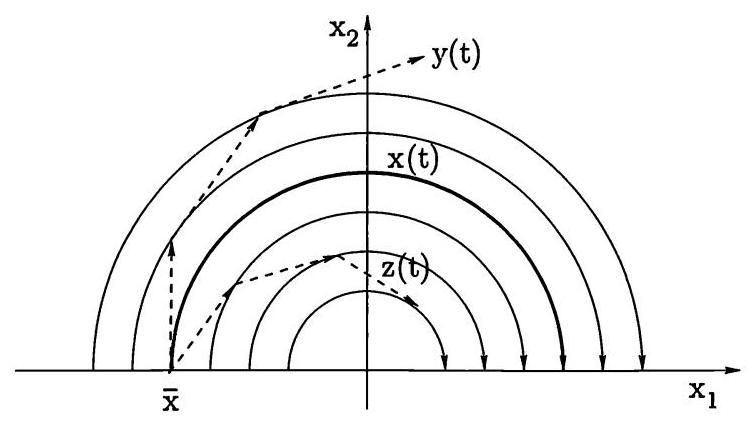
\includegraphics[width=0.7\textwidth]{images/bo_d6ik6nn7aajc739ct1l0_129_334_235_748_423_0.jpg}
\caption{系统 ${\dot{x}}_{1} = {x}_{2},{\dot{x}}_{2} = \; - {x}_{1}$ 的 Euler 近似.其中 $x\left( \cdot \right)$ 为精确解， $y\left( \cdot \right)$ 是由前向 Euler 格式得到的分段仿射近似，而 $z\left( \cdot \right)$ 是由后向 Euler 格式得到.}
\label{fig:euler-approximation}
\end{figure}

— 前向 Euler 近似:近似解在时刻 ${t}_{j}$ 的取值按如下公式归纳定义
\begin{equation}\tag{7.6}\label{eq:forward-euler}
x\left( {t}_{j + 1}\right)  = x\left( {t}_{j}\right)  + {hF}\left( {x\left( {t}_{j}\right) }\right) .
\end{equation}

— 后向 Euler 近似:近似解在时刻 ${t}_{j}$ 的取值由下式确定
\begin{equation}\tag{7.7}\label{eq:backward-euler}
x\left( {t}_{j + 1}\right)  = x\left( {t}_{j}\right)  + {hF}\left( {x\left( {t}_{j + 1}\right) }\right) .
\end{equation}

两种情形下，一旦在离散时刻集 ${t}_{j}$ 上计算出 $x\left( {t}_{j}\right)$ 的值，即可将近似解延拓至所有实数 $t \geq  0$ ，令 $t \mapsto  x\left( t\right)$ 在每个区间 $\left(  {{t}_{j - 1},{t}_{j}}\right)$ 上为仿射函数.

前向 Euler 近似易于构造:在整个时间区间 $\left(  {{t}_{j},{t}_{j + 1}}\right)$ 上，令导数 $\dot{x}\left( t\right)$ 保持恒定，且等于初值点处 $F$ 的取值:
\[
\dot{x}\left( t\right)  = F\left( {x\left( {t}_{j}\right) }\right) ,\;t \in  \left(  {{t}_{j},{t}_{j + 1}}\right)  .
\]

另一方面，在后向Euler近似中，对于 $t \in  \left(  {{t}_{j},{t}_{j + 1}}\right)$ ，我们令导数 $\dot{x}\left( t\right)$ 保持恒定，且等于 $F$ 在终点处的值:
\[
\dot{x}\left( t\right)  = F\left( {x\left( {t}_{j + 1}\right) }\right) ,\;t \in  \left(  {{t}_{j},{t}_{j + 1}}\right)  .
\]

此时，给定 $x\left( {t}_{j}\right)$ ，为求得 $x\left( {t}_{j + 1}\right)$ ，需求解隐式方程\eqref{eq:backward-euler}.因此，后向Euler近似需要更多的计算工作量；但另一方面，其通常具有更优的稳定性和收敛性.

\subsection{线性齐次常微分方程}

设 $A : {\mathbb{R}}^{n} \mapsto  {\mathbb{R}}^{n}$ 为一线性算子.则线性Cauchy问题的解
\begin{equation}\tag{7.8}\label{eq:linear-ode}
\dot{x} = {Ax},\;x\left( 0\right)  = \bar{x}
\end{equation}

是映射 $t \mapsto  {e}^{tA}\bar{x}$ ，其中
\begin{equation}\tag{7.9}\label{eq:exp-series}
{e}^{tA} \doteq  \mathop{\sum }\limits_{{k = 0}}^{\infty }\frac{{t}^{k}{A}^{k}}{k!}
\end{equation}

该公式对任意Banach空间 $X$ 上的有界线性算子 $A$ 依然成立.我们注意到，\eqref{eq:exp-series}式中的级数对每个 $t \in  \mathbb{R}$ 均绝对收敛.此外，指数映射具有如下性质:

(i) ${e}^{0A} = I$ ，即恒等映射.

(ii) ${e}^{sA}{e}^{tA} = {e}^{\left( {s + t}\right) A}$ (半群性质).

(iii) 对每个 $\bar{x} \in  X$ ，映射 $t \mapsto  {e}^{tA}\bar{x}$ 连续.

由 (i)-(ii) 可知，算子族 $\left\{  {{e}^{tA};t \geq  0}\right\}$ 构成一个线性算子群.

更一般地，线性半群理论研究线性算子与其指数之间的对应关系.
\[
A \leftrightarrow  \left\{  {{e}^{tA};t \geq  0}\right\}
\]

当 $A$ 为有界线性算子时，其指数函数由收敛级数\eqref{eq:exp-series}给出.反之，给定算子族 ${e}^{tA}$，可通过极限恢复 $A$
\[
A = \mathop{\lim }\limits_{{t \rightarrow  0 + }}\frac{{e}^{tA} - I}{t}.
\]

存在重要情形:对每个 $t \geq  0$ ，算子 ${e}^{tA}$ 均有界，而 $A$ 却是无界算子.这恰是半群理论最具意义的应用，广泛用于抛物型或双曲型偏微分方程的分析.

\begin{instance}\label{ins:diagonal-matrix-exponential}
若 $A : {\mathbb{R}}^{n} \mapsto  {\mathbb{R}}^{n}$ 为一对角矩阵，则其指数可直接计算.事实上
\[
A = \left( \begin{matrix} {\lambda }_{1} & & 0 \\  \vdots & & \vdots \\  0 & & {\lambda }_{n} \end{matrix}\right) ,\;{e}^{tA} = \left( \begin{matrix} {e}^{t{\lambda }_{1}} & & 0 \\  \vdots & & \vdots \\  0 & & {e}^{t{\lambda }_{n}} \end{matrix}\right) .
\]

注意，对应的算子范数为
\[
\| A\| \; = \;\mathop{\max }\limits_{k}\;\left| {\lambda }_{k}\right| ,\;\| {e}^{tA}\| \; = \;\mathop{\max }\limits_{k}\left| {e}^{t{\lambda }_{k}}\right| .
\]
\end{instance}

\begin{instance}\label{ins:diagonal-operator-l1}
设 ${\ell }^{1}$ 为赋范为 $x = \left( {{x}_{1},{x}_{2},{x}_{3},\ldots }\right)$ 的复数序列全体构成的Banach空间
\[
\| x{\| }_{{\ell }^{1}} \doteq  \mathop{\sum }\limits_{k}\left| {x}_{k}\right|
\]

对任意复数序列 ${\left( {\lambda }_{k}\right) }_{k \geq  1}$ ，考虑线性算子
\begin{equation}\tag{7.10}\label{eq:diagonal-operator-l1}
{Ax} \doteq  \left( {{\lambda }_{1}{x}_{1},{\lambda }_{2}{x}_{2},{\lambda }_{3}{x}_{3},\ldots }\right) .
\end{equation}

相应的指数算子为
\[
{e}^{tA}x = \left( {{e}^{t{\lambda }_{1}}{x}_{1},{e}^{t{\lambda }_{2}}{x}_{2},{e}^{t{\lambda }_{3}}{x}_{3},\ldots }\right) .
\]

需注意，该量
\[
\| A\|  = \mathop{\sup }\limits_{k}\left| {\lambda }_{k}\right|
\]
可能为无穷大，但与此同时，范数
\[
\norm{e}^{tA} = \mathop{\sup }\limits_{k}\left| {e}^{t{\lambda }_{k}}\right|
\]
对每个 $t \geq  0$ 均可有界.事实上，如图\ref{fig:spectrum-regions}所示，假设所有特征值 ${\lambda }_{k}$ 的实部一致上有界，即
\[
{\lambda }_{k} = {\alpha }_{k} + i{\beta }_{k},\;{\alpha }_{k} \leq  \omega \;\forall\,k \geq  1,
\]

对某个常数 $\omega  \in  \mathbb{R}$ 成立.则
\begin{equation}\tag{7.11}\label{eq:exp-bound-semigroup}
\left| {e}^{t{\lambda }_{k}}\right|  = \left| {e}^{t{\alpha }_{k}}\right|  \leq  {e}^{t\omega }\;\forall\,t \geq  0.
\end{equation}

因此，对每个 $t \geq  0$ ，算子 ${e}^{tA}$ 均有界，即 $\norm{e}^{tA} \leq  {e}^{t\omega }$ .

另两种情形亦值得探讨.

情形1:假设所有特征值 ${\lambda }_{k}$ 的实部既有上界也有下界，即
\[
- \omega  \leq  {\alpha }_{k} \leq  \omega
\]

对某个常数 $\omega  > 0$ 及所有 $k \geq  1$ 成立.则对所有 $t \in  \mathbb{R}$ ，有估计式
\begin{equation}\tag{7.12}\label{eq:exp-bound-group}
\left| {e}^{t{\lambda }_{k}}\right|  = \left| {e}^{t{\alpha }_{k}}\right|  \leq  {e}^{\left| t\right| \omega }
\end{equation}

故算子 ${e}^{tA}$ 对所有 $t < 0$ 均有界.这表明微分方程\eqref{eq:linear-ode}既可正向也可反向求解.算子族 $\left\{  {{e}^{tA};t \in  \mathbb{R}}\right\}$ 构成一族有界线性算子群.

情形2:假设所有特征值 ${\lambda }_{k} = {\alpha }_{k} + i{\beta }_{k}$ 均位于复平面的一个扇形区域内.更准确地说，假设存在 $\omega  \in  \mathbb{R}$ 与角度 $0 < \overline{\theta } < \pi /2$ ，使得对每个 $k$ ，可写为
\begin{equation}\tag{7.13}\label{eq:sectorial-eigs}
{\alpha }_{k} = \omega  - {r}_{k}\cos {\theta }_{k},\;{\beta }_{k} =  - {r}_{k}\sin {\theta }_{k}
\end{equation}

其中 ${r}_{k} \geq  0$ 与 ${\theta }_{k} \in  \left(  {-\overline{\theta },\overline{\theta }}\right)$ 为某常数.

此时，由于 ${\alpha }_{k} \leq  \omega$ ，显然\eqref{eq:exp-bound-semigroup}成立，且算子 $\norm{e}^{tA}$ 对每个 $t \geq  0$ 均有界.然而，更强的结论成立:对每个 $t > 0$ ，复合算子 $A{e}^{tA}$ 均有界.事实上
{\begin{align*}
    \norm{A{e}^{tA}} &= \mathop{\sup }\limits_{k}\left| {{\lambda }_{k}{e}^{t{\lambda }_{k}}}\right|  \leq  \mathop{\sup }\limits_{k}\left( {\omega  + {r}_{k}}\right) {e}^{\left( {\omega  - {r}_{k}\cos {\theta }_{k}}\right) t}\\
    &\leq  \mathop{\sup }\limits_{{r \geq  0,\left| \theta \right|  \leq  \overline{\theta }}}\left( {\omega  + r}\right) {e}^{\left( {\omega  - r\cos \theta }\right) t} \leq  \mathop{\sup }\limits_{{r \geq  0}}\left( {\omega  + r}\right) {e}^{\left( {\omega  - r\cos \overline{\theta }}\right) t} <  + \infty ,
\end{align*}}

因为 $\cos \overline{\theta } > 0$ .此时， $A$ 称为扇形算子.

即使初始数据 $\bar{x}$ 不在算子 $A$ 的定义域内，对每个 $t > 0$ ，仍有 $x\left( t\right)  = {e}^{tA}\bar{x} \in  \operatorname{Dom}\left( A\right)$ .

\begin{figure}[htbp]
\centering
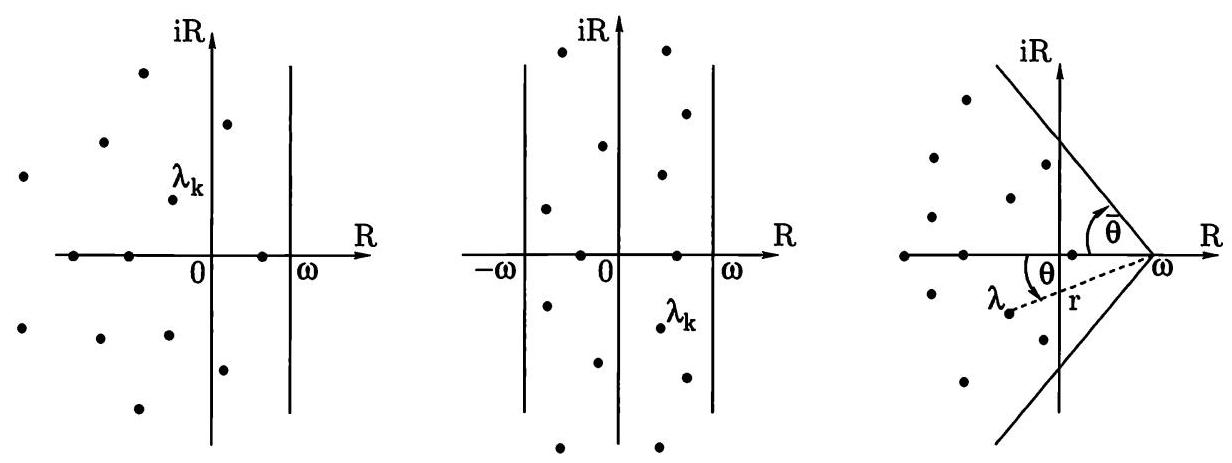
\includegraphics[width=1.0\textwidth]{images/bo_d6ik6nn7aajc739ct1l0_132_122_1026_1232_463_0.jpg}
\caption{左:当算子 $A$ (见\eqref{eq:diagonal-operator-l1}式)的所有特征值 ${\lambda }_{k}$ 的实部满足 $\operatorname{Re}\left( {\lambda }_{k}\right)  \leq  \omega$ 时，则对每个 $t \geq  0$ ，指数算子均有界: $\norm{e}^{tA} \leq  {e}^{t\omega }$ .中:若所有特征值 ${\lambda }_{k}$ 满足 $\operatorname{Re}\left( {\lambda }_{k}\right)  \in  \left(  {-\omega ,\omega }\right)$ ，则对每个 $t \in  \mathbb{R}$ ，指数算子均有界: $\norm{e}^{tA} \leq  {e}^{\left| t\right| \omega }$ .右:若所有特征值 ${\lambda }_{k}$ 位于复平面中一个张角为 $\overline{\theta } < \pi /2$ 的扇形内，则对每个 $t > 0$ ，算子 $A{e}^{tA}$ 同样有界.}
\label{fig:spectrum-regions}
\end{figure}
\end{instance}

\section{线性算子半群}

考虑Banach空间 $X$ 中的线性演化方程，例如
\begin{equation}\tag{7.14}\label{eq:evolution-equation}
\frac{\d}{\d t}u\left( t\right)  = {Au}\left( t\right) ,\;u\left( 0\right)  = \bar{u} \in  X.
\end{equation}

当$t \geq  0$ ，我们希望将解表示为$u\left( t\right)  = {e}^{tA}\bar{u}$ ，其中 $\left\{  {{e}^{tA};t \geq  0}\right\}$ 是一族线性算子.

\begin{instance}\label{ins:transport-equation}
考虑偏微分方程 ${u}_{t} - {u}_{x} = 0$ .该方程可重写为形式\eqref{eq:evolution-equation}，其中 $A = \frac{\partial }{\partial x}$ 是一个微分算子.作为函数空间，可取 $X = {L}^{p}\left( \mathbb{R}\right)$ ，其中 $p \in (1,\infty)$ 为某常数.显然，微分算子 $A$ 是无界的，其定义域为所有绝对连续函数 $u \in  {L}^{p}\left( \mathbb{R}\right)$ ，且其导数 ${u}_{x} \in  {L}^{p}\left( \mathbb{R}\right)$ 满足相应条件.另一方面，对任意初值 $\bar{u} \in  {L}^{p}$ ，初值问题的解
\[
{u}_{t} = {u}_{x},\;u\left( {0,x}\right)  = \bar{u}\left( x\right)
\]

可显式计算:
\[
u\left( {t,x}\right)  = \bar{u}\left( {x + t}\right) ,\;t \in  \mathbb{R}.
\]

这表明，尽管微分算子 $A = \frac{\partial }{\partial x}$ 是无界的，相应的指数算子 ${e}^{tA}$ 却是一致有界的:
\[
\left( {{e}^{tA}\bar{u}}\right) \left( x\right)  = \bar{u}\left( {x + t}\right)
\]
从而对每个 $t \in  \mathbb{R}$ 均有 $\norm{e}^{tA} = 1$ .
\end{instance}

在线性半群理论中，需考虑两个基本问题:

\begin{enumerate}[(1)]
    \item 给定一族线性算子半群 $\left\{  {{S}_{t};t \geq  0}\right\}$ ，求其生成元，即求算子$A$ ，使得${S}_{t} = {e}^{tA}$.
    \item 给定一线性算子 $A$ ，判断它是否生成一个半群 $\left\{  {{e}^{tA};t \geq  0}\right\}$ ，并研究其性质.
\end{enumerate}

在应用中，(2)显然更为重要；然而，为推进理论发展，从(1)入手则更为方便.

\subsection{半群的定义与基本性质}

\begin{definition}[强连续线性算子半群]\label{def:C0-semigroup}
设 $X$ 为一Banach空间. $X$ 上的\colorbf{强连续线性算子半群}是指一族线性映射 $\left\{  {{S}_{t};t \geq  0}\right\}$，满足如下性质.
\begin{enumerate}[(i)]
    \item 每个 ${S}_{t} : X \mapsto  X$ 均为有界线性算子.
    \item 对任意 $s,t \geq  0$ ，复合运算满足 ${S}_{t}{S}_{s} = {S}_{t + s}$；且 ${S}_{0} = I$.
    \item 对任意 $u \in  X$ ，映射 $t \mapsto  {S}_{t}u$ 是从 $(0,\infty )$ 到 $X$ 的连续映射.
\end{enumerate}
\end{definition}
\begin{definition}[$\omega$类算子半群]\label{def:semigroup-type}
    若强连续线性算子半群满足如下估计式：
    \begin{equation}\tag{7.15}\label{eq:semigroup-type}
\norm{S}_{t} \leq  {e}^{t\omega }\;\forall\,t \geq  0.
\end{equation}
    则称 $\left\{  {{S}_{t};t \geq  0}\right\}$ 为\colorbf{$\omega$类算子半群}.\par
    特别地，当$\omega = 0$时，称$\left\{{{S}_{t};t \geq  0}\right\}$为\colorbf{压缩算子半群}.
\end{definition}
事实上，对压缩算子半群，对于每个 $t \geq  0$ 均有 $\norm{S}_{t} \leq  1$ ，故
\[
\norm{{S}_{t}u - {S}_{t}v} \leq  \| u - v\| \;\forall\,\;u,v \in  X,t \geq  0.
\]
\begin{definition}[算子半群的生成元]
    线性算子
\begin{equation}\tag{7.16}\label{eq:generator-def}
{Au} \doteq  \mathop{\lim }\limits_{{t \rightarrow  0 + }}\frac{{S}_{t}u - u}{t}
\end{equation}
称为半群 $\left\{  {{S}_{t};t \geq  0}\right\}$ 的\colorbf{生成元}.其定义域 $\operatorname{Dom}\left( A\right)$ 是使\eqref{eq:generator-def}中极限存在的所有 $u \in  X$ 构成的集合.
\end{definition}



对给定的 $\bar{u} \in  X$ ，我们将映射 $t \mapsto  {S}_{t}\bar{u}$ 视为线性常微分方程\eqref{eq:evolution-equation}的解.注意，此处在某种意义上我们是逆向处理该问题:给定解 $u\left( t\right)  = {S}_{t}\bar{u}$ ，我们试图重构演化方程，并找出算子 $A$ .接下来推导半群 $S$ 及其生成元 $A$ 的若干基本性质.


\begin{theorem}[半群的性质]\label{thm:semigroup-properties}
设 $\left\{  {{S}_{t};t \geq  0}\right\}$ 是强连续半群， $A$ 为其生成元，且假设 $\bar{u} \in  \operatorname{Dom}\left( A\right)$ .则
\begin{enumerate}[(i)]
    \item 对每个 $t \geq  0$ ，均有 ${S}_{t}\bar{u} \in  \operatorname{Dom}\left( A\right)$ 且 $A{S}_{t}\bar{u} = {S}_{t}A\bar{u}$.
    \item 映射 $t \mapsto  u\left( t\right)  \doteq  {S}_{t}\bar{u}$ 连续可微，且为初值问题\eqref{eq:evolution-equation}的解.
\end{enumerate}
\end{theorem}

\begin{proof}
1. 设 $\bar{u} \in  \operatorname{Dom}\left( A\right)$ ，即\eqref{eq:generator-def}中的极限存在.则
\[
\mathop{\lim }\limits_{{s \rightarrow  0 + }}\frac{{S}_{s}{S}_{t}\bar{u} - {S}_{t}\bar{u}}{s} = \mathop{\lim }\limits_{{s \rightarrow  0 + }}\frac{{S}_{t}{S}_{s}\bar{u} - {S}_{t}\bar{u}}{s} = {S}_{t}\mathop{\lim }\limits_{{s \rightarrow  0 + }}\frac{{S}_{s}\bar{u} - \bar{u}}{s} = {S}_{t}A\bar{u}.
\]

因此 ${S}_{t}\bar{u} \in  \operatorname{Dom}\left( A\right)$ 且 $A{S}_{t}\bar{u} = {S}_{t}A\bar{u}$ ，从而证得(i).

\noindent 2. 接着，设 $\bar{u} \in  \operatorname{Dom}\left( A\right) ,t > 0$ .由半群性质可得
\begin{gather*}
\mathop{\lim }\limits_{{h \rightarrow  0 + }}\left\{  {\frac{{S}_{t}\bar{u} - {S}_{t - h}\bar{u}}{h} - {S}_{t}A\bar{u}}\right\}   = \mathop{\lim }\limits_{{h \rightarrow  0 + }}\left\{  {{S}_{t - h}\left( \frac{{S}_{t - h}\bar{u} - \bar{u}}{h}\right)  - {S}_{t}A\bar{u}}\right\}\\
= \mathop{\lim }\limits_{{h \rightarrow  0 + }}\left\{  {{S}_{t - h}\left( {\frac{{S}_{h}\bar{u} - \bar{u}}{h} - A\bar{u}}\right)  + \left( {{S}_{t - h}A\bar{u} - {S}_{t}A\bar{u}}\right) }\right\}   = 0.
\end{gather*}

事实上， $\frac{{S}_{h}\bar{u} - \bar{u}}{h} \rightarrow  A\bar{u}$ ，而 $\norm{S}_{t - h} \leq  {e}^{t\omega }$ .此外，由于 $A\bar{u} \in  X$ 定义良好，映射 $s \mapsto  {S}_{s}A\bar{u}$ 连续.上述计算表明，映射 $t \mapsto  u\left( t\right)  = {S}_{t}\bar{u}$ 存在左导数:
\[
\mathop{\lim }\limits_{{h \rightarrow  0 + }}\frac{{S}_{t}\bar{u} - {S}_{t - h}\bar{u}}{h} = {S}_{t}A\bar{u}.
\]

右导数计算如下:
\[
\mathop{\lim }\limits_{{h \rightarrow  0 + }}\frac{{S}_{t + h}\bar{u} - {S}_{t}\bar{u}}{h} = {S}_{t}\mathop{\lim }\limits_{{h \rightarrow  0 + }}\frac{{S}_{h}\bar{u} - \bar{u}}{h} = {S}_{t}A\bar{u}.
\]

因此，对每个 $t > 0$ ，映射 $t \mapsto  {S}_{t}\bar{u}$ 可微，且其导数为 $\frac{\d}{\d t}{S}_{t}\bar{u} = {S}_{t}A\bar{u} = A{S}_{t}\bar{u}$ .又因 $A\bar{u} \in  X$ ，依半群定义，映射 $t \mapsto  {S}_{t}\left( {A\bar{u}}\right)$ 必连续，故映射 $t \mapsto  {S}_{t}\bar{u}$ 连续可微.
\end{proof}

以下定理汇总生成元 $A$ 的若干性质.我们回顾:若线性算子 $A : X \mapsto  X$ 的图像
\[
\operatorname{Graph}\left( A\right)  = \{ \left( {x,y}\right)  \in  X \times  X;x \in  \operatorname{Dom}\left( A\right) ,y = {Ax}\}
\]
是乘积空间 $X \times  X$ 中的闭集，则称其为闭算子.

\begin{theorem}[生成元的性质]\label{thm:generator-properties}
设 $\left\{  {{S}_{t};t \geq  0}\right\}$ 是 Banach 空间 $X$ 上的强连续半群，其生成元为 $A$ .则
\begin{enumerate}[(i)]
    \item $A$ 的定义域在 $X$ 中稠密.
    \item 算子 $A$ 是闭的.
\end{enumerate}
\end{theorem}

\begin{proof}
1. 任取 $u \in  X$ ，考虑逼近 ${U}_{\varepsilon } \doteq  {\varepsilon }^{-1}{\int }_{0}^{\varepsilon }{S}_{s}{u\d s}$ .由于映射 $t \mapsto  {S}_{t}u$ 连续，故当 $\varepsilon  \rightarrow  0 +$ 时有 ${U}_{\varepsilon } \rightarrow  u$ .为证 (i)，现证对每个 $\varepsilon  > 0$ 均有 ${U}_{\varepsilon } \in  \operatorname{Dom}\left( A\right)$ .因 $\operatorname{Dom}\left( A\right)$ 是向量子空间，只需证
\[
{u}_{\varepsilon } \doteq  \varepsilon {U}_{\varepsilon } = {\int }_{0}^{\varepsilon }{S}_{s}{u\d s} \in  \operatorname{Dom}\left( A\right) .
\]

对 $0 < h < \varepsilon$ ，有
{\begin{align*}
    \frac{{S}_{h}{u}_{\varepsilon } - {u}_{\varepsilon }}{h} &= \frac{1}{h}\left\{  {{S}_{h}\left( {{\int }_{0}^{\varepsilon }{S}_{s}{u\d s}}\right)  - \left( {{\int }_{0}^{\varepsilon }{S}_{s}{u\d s}}\right) }\right\}\\
    &= \frac{1}{h}{\int }_{0}^{\varepsilon }\left( {{S}_{s + h}u - {S}_{s}u}\right) {\d s}\\
    &= \frac{1}{h}{\int }_{\varepsilon }^{\varepsilon  + h}{S}_{s}{u\d s} - \frac{1}{h}{\int }_{0}^{h}{S}_{s}{u\d s} \rightarrow  {S}_{\varepsilon }u - u\;\;\text{当}h \rightarrow  0 +
\end{align*}}

这表明对每个 $\varepsilon  > 0$ 均有 ${u}_{\varepsilon } \in  \operatorname{Dom}\left( A\right)$ ，从而证得 (i).

\noindent 2. 接下来证明 $A$ 的图像闭.设 $\left( {{u}_{k},{v}_{k}}\right)$ 是 $A$ 图像上的一列点.更准确地说，设 ${u}_{k} \in  \operatorname{Dom}A,{v}_{k} = A{u}_{k}$ ，并假设收敛 ${u}_{k} \rightarrow  u,{v}_{k} \rightarrow  v$ (其中 $u,v \in  X$ 为某元素).需证 $u \in  \operatorname{Dom}\left( A\right)$ 且 ${Au} = v$ .对每个 $k \geq  1$ ，由于 ${u}_{k} \in  \operatorname{Dom}\left( A\right)$ ，由定理\ref{thm:semigroup-properties}推出
\[
{S}_{h}{u}_{k} - {u}_{k} = {\int }_{0}^{h}\left( {\frac{\d}{\d t}{S}_{t}{u}_{k}}\right) {\d t} = {\int }_{0}^{h}{S}_{t}A{u}_{k}{\d t}
\]

令 $k \rightarrow  \infty$ ，得
\[
{S}_{h}u - u = {\int }_{0}^{h}{S}_{t}{v\d t}
\]

因此，
\[
\mathop{\lim }\limits_{{h \rightarrow  0 + }}\frac{{S}_{h}u - u}{h} = \mathop{\lim }\limits_{{h \rightarrow  0 + }}\frac{1}{h}{\int }_{0}^{h}{S}_{t}{v\d t} = v
\]

由定义，这意味着 $u \in  \operatorname{Dom}\left( A\right)$ 且 ${Au} = v$ .
\end{proof}

\begin{figure}[htbp]
\centering
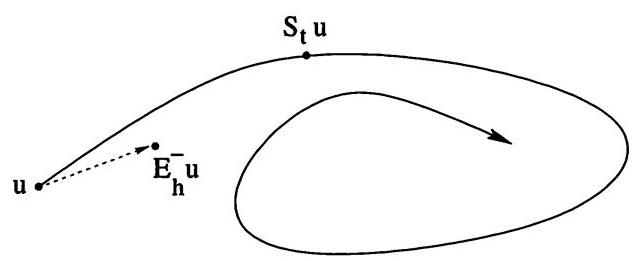
\includegraphics[width=0.6\textwidth]{images/bo_d6ik6nn7aajc739ct1l0_136_739_911_639_261_0.jpg}
\caption{右:依据\eqref{eq:scalar-backward-euler-average}或\eqref{eq:backward-euler-average}，步长为 $h > 0$ 的后向 Euler 逼近是轨迹 $t \mapsto  {S}_{t}u$ 上各点的加权平均，权重呈指数衰减 $w\left( t\right)  = {e}^{-t/h}/h$.}
\label{fig:generator-density}
\end{figure}

\section{预解式}

半群 $\left\{  {{S}_{t};t \geq  0}\right\}$ 与其生成元 $A$ 之间的关键联系由所谓“预解式”给出.该概念借助后向 Euler 逼近最易理解.

假设我们欲用后向Euler逼近近似求解\eqref{eq:evolution-equation}.于是固定时间步长$h > 0$ ，并迭代求解
\[
u\left( {t + h}\right)  = u\left( t\right)  + {hAu}\left( {t + h}\right) .
\]

在每一步中，给定值 $u\left( t\right)  \in  X$ ，我们需计算
\[
u\left( {t + h}\right)  = {\left( I - hA\right) }^{-1}u\left( t\right) .
\]

后向Euler算子
\begin{equation}\tag{7.17}\label{eq:backward-euler-operator}
{E}_{h}^{ - } \doteq  {\left( I - hA\right) }^{-1}
\end{equation}

当 $h > 0$ 较小时，该算子在半群理论中起着关键作用.给定 $A$ ，可通过该算子以两种主要方式恢复Cauchy问题\eqref{eq:evolution-equation}的解.

\subsection{作为后向Euler逼近的极限}

对固定的$\tau  > 0$，考虑时间步长 $h = \tau /n$ .经过 $n$ 步后，后向Euler逼近格式给出
\[
u\left( \tau \right)  \approx  {E}_{\tau /n}^{ - } \circ  \cdots  \circ  {E}_{\tau /n}^{ - } = {\left( I - \frac{\tau }{n}A\right) }^{-n}\bar{u}.
\]

保持 $\tau$ 固定并令 $n \rightarrow  \infty$ ，我们期望在极限下恢复\eqref{eq:evolution-equation}的精确解:
\begin{equation}\tag{7.18}\label{eq:backward-euler-limit}
u\left( \tau \right)  = {S}_{\tau }\bar{u} \doteq  \mathop{\lim }\limits_{{n \rightarrow  \infty }}{\left( I - \frac{\tau }{n}A\right) }^{-n}\bar{u}.
\end{equation}

\subsection{作为近似演化方程解的极限}

再次固定时间步长 $h > 0$ ，并设 $\lambda  = 1/h$ .然后将算子 ${A}_{\lambda } : X \mapsto  X$ 定义为
\[
{A}_{\lambda }u \doteq  A{E}_{h}^{ - }u = A{\left( I - hA\right) }^{-1}u.
\]

换言之， ${A}_{\lambda }u$ 是 $A$ 在 $u$ 处的取值，而非在 ${E}_{h}^{ - }u$ 处，即在后向Euler逼近的第一步中、取 $h = 1/\lambda$ 时的值.事实表明，当 $h > 0$ 足够小时， ${A}_{\lambda } = {A}_{1/h}$ 是一个定义良好且有界的线性算子.因此，我们可以考虑指数型算子 ${e}^{t{A}_{\lambda }} = \mathop{\sum }\limits_{{k \geq  0}}{\left( t{A}_{\lambda }\right) }^{k}/k$ ！并定义
\begin{equation}\tag{7.19}\label{eq:exponential-approx-limit}
u\left( t\right)  = {S}_{t}\bar{u} \doteq  \mathop{\lim }\limits_{{\lambda  \rightarrow  \infty }}{e}^{t{A}_{\lambda }}\bar{u}.
\end{equation}

\begin{instance}\label{ins:scalar-euler}
考虑标量常微分方程
\[
\dot{x} = {ax},\;x\left( 0\right)  = \bar{x}.
\]

其解为 $x\left( t\right)  = {e}^{ta}\bar{x}$ .此时我们平凡地有
\[
{a}_{\lambda } = {a}_{1/h} = \frac{a}{1 - {ha}},\;{e}^{at}\bar{x} = \mathop{\lim }\limits_{{h \rightarrow  0}}{e}^{t{a}_{1/h}}\bar{x} = \mathop{\lim }\limits_{{h \rightarrow  0 + }}{e}^{{ta}/\left( {1 - {ha}}\right) }\bar{x}.
\]

这对应于极限\eqref{eq:exponential-approx-limit}.另一方面，极限\eqref{eq:backward-euler-limit}与恒等式相关
\[
{e}^{\tau a} = \mathop{\lim }\limits_{{n \rightarrow  \infty }}{\left( 1 - \frac{\tau }{n}a\right) }^{-n}
\]

注意，当 $0 < h < {a}^{-1}$ 时，还成立如下恒等式
\begin{equation}\tag{7.20}\label{eq:scalar-backward-euler-average}
{\int }_{0}^{\infty }\frac{{e}^{-t/h}}{h}{\d t} = 1,\;{\left( 1 - ha\right) }^{-1}\bar{x} = {\int }_{0}^{\infty }\left( \frac{{e}^{-t/h}}{h}\right) {e}^{ta}\bar{x}{\d t}.
\end{equation}

第二个恒等式表明，后向Euler算子 ${E}_{h}^{ - }\bar{x} = \; {\left( 1 - ha\right) }^{-1}\bar{x}$ 可通过沿轨迹 $t \mapsto  {e}^{ta}\bar{x}$ 取点并赋予指数衰减权重 $w\left( t\right)  = {h}^{-1}{e}^{-t/h}$ 进行加权平均而得到.
\end{instance}

受前述分析启发，我们引入若干定义.

\begin{definition}[预解集与预解算子]\label{def:resolvent}
设 $A$ 为Banach空间 $X$ 上的线性算子. $A$ 的\colorbf{预解集}是使得算子
\[
{\lambda I} - A : \operatorname{Dom}\left( A\right)  \mapsto  X
\]
是单射且满射的所有实数 $\lambda$ 构成的集合 $\rho \left( A\right)$.\par
若 $\lambda  \in  \rho \left( A\right)$ ，则\colorbf{预解算子}${R}_{\lambda } : X \mapsto  X$ 定义为
\[
{R}_{\lambda }u \doteq  {\left( \lambda I - A\right) }^{-1}u
\]
\end{definition}
我们指出，若 $A$ 是闭算子，则由闭图像定理可知，算子 ${R}_{\lambda } : X \mapsto  \operatorname{Dom}\left( A\right)  \subseteq  X$ 是有界线性算子.此外
\[
A{R}_{\lambda }u = {R}_{\lambda }{Au}\;\text{ if }u \in  \operatorname{Dom}\left( A\right) .
\]

预解式与后向Euler算子之间存在紧密联系.即
\[
\lambda {R}_{\lambda } = {E}_{1/\lambda }^{ - }
\]

\begin{theorem}[预解式恒等式]\label{thm:resolvent-identities}
设 $A$ 为闭线性算子.若 $\lambda ,\mu  \in  \rho \left( A\right)$ ，则
\begin{equation}\tag{7.21}\label{eq:resolvent-identity}
{R}_{\lambda } - {R}_{\mu } = \left( {\mu  - \lambda }\right) {R}_{\lambda }{R}_{\mu }
\end{equation}
\vspace{-2.2 em}
\begin{equation}\tag{7.22}\label{eq:resolvent-commute}
{R}_{\lambda }{R}_{\mu } = {R}_{\mu }{R}_{\lambda }
\end{equation}
\end{theorem}
\begin{proof}
对任意 $u \in  X$ ，有
\[
v \doteq  {R}_{\lambda }u - {R}_{\mu }u = {\left( \lambda I - A\right) }^{-1}u - {\left( \mu I - A\right) }^{-1}u \in  \operatorname{Dom}\left( A\right) ,
\]

$\left( {{\lambda I} - A}\right) v = u - \left( {{\lambda I} - {\mu I} + {\mu I} - A}\right) {\left( \mu I - A\right) }^{-1}u = \left( {\mu  - \lambda }\right) {\left( \mu I - A\right) }^{-1}u.$\par
将算子 ${\left( \lambda I - A\right) }^{-1}$ 作用于上述恒等式两边，即得\eqref{eq:resolvent-identity}.

接下来，利用\eqref{eq:resolvent-identity}，对预解集 $\rho \left( A\right)$ 中的任意 $\lambda  \neq  \mu$ ，可得
\[
{R}_{\lambda }{R}_{\mu } = \frac{{R}_{\lambda } - {R}_{\mu }}{\lambda  - \mu } = \frac{{R}_{\mu } - {R}_{\lambda }}{\mu  - \lambda } = {R}_{\mu }{R}_{\lambda }.
\]
\end{proof}

\begin{theorem}[预解式的积分表达式]\label{thm:resolvent-integral}
设 $\left\{  {{S}_{t};t \geq  0}\right\}$ 是$\omega$类半群，其生成元为 $A$ .则对每个 $\lambda  > \omega$，均有 $\lambda  \in  \rho \left( A\right)$ ，且
\begin{equation}\tag{7.23}\label{eq:resolvent-integral-formula}
{R}_{\lambda }u = {\int }_{0}^{\infty }{e}^{-{t\lambda }}{S}_{t}{u\d t}
\end{equation}

此外，
\begin{equation}\tag{7.24}\label{eq:resolvent-bound}
\norm{R}_{\lambda } \leq  \frac{1}{\lambda  - \omega }
\end{equation}


\end{theorem}
\begin{proof}
1. 由假设，该半群满足估计式 $\norm{S}_{t} \leq  {e}^{t\omega }$ .因此\eqref{eq:resolvent-integral-formula}中的积分绝对收敛:
\begin{equation}\tag{7.25}\label{eq:resolvent-integral-estimate}
\norm{{\int }_{0}^{\infty }{e}^{-{t\lambda }}{S}_{t}{u\d t}} \leq  {\int }_{0}^{\infty }{e}^{t\lambda }\norm{S}_{t}\| u\| {\d t} \leq  {\int }_{0}^{\infty }{e}^{\left( {\omega  - \lambda }\right) t}\| u\| {\d t} \leq  \frac{1}{\lambda  - \omega }\| u\| .
\end{equation}

定义
\[
{\widetilde{R}}_{\lambda }u \doteq  {\int }_{0}^{\infty }{e}^{-{t\lambda }}{S}_{t}{u\d t}
\]

上述估计表明 ${\widetilde{R}}_{\lambda }$ 是有界线性算子，其范数为
\[
\norm{\widetilde{R}}_{\lambda } \leq  \frac{1}{\lambda  - \omega }
\]

\noindent 2. 我们现证
\begin{equation}\tag{7.26}\label{eq:resolvent-surjective}
\left( {{\lambda I} - A}\right) {\widetilde{R}}_{\lambda }u = u\;\forall\,u \in  X.
\end{equation}

事实上，对任意 $h > 0$ ，有
{\begin{align*}
    \frac{{S}_{h}{\widetilde{R}}_{\lambda }u - {\widetilde{R}}_{\lambda }u}{h} &= \frac{1}{h}{\int }_{0}^{\infty }{e}^{-{\lambda t}}\left( {{S}_{t + h}u - {S}_{t}u}\right) {\d t} \\
    &= \frac{1}{h}{\int }_{0}^{\infty }\left( {{e}^{-\lambda \left( {t - h}\right) } - {e}^{-{\lambda t}}}\right) {S}_{t}{u\d t} - \frac{1}{h}{\int }_{0}^{h}{e}^{-\lambda \left( {t - h}\right) }{S}_{t}{u\d t} \\
    &= \left( \frac{{e}^{\lambda h} - 1}{h}\right) {\int }_{0}^{\infty }{e}^{-{\lambda t}}{S}_{t}{u\d t} - \frac{{e}^{\lambda h}}{h}{\int }_{0}^{h}{e}^{-{\lambda t}}{S}_{t}{u\d t}.
\end{align*}}
令 $h \rightarrow  0 +$ 取极限，得
\[
\mathop{\lim }\limits_{{h \rightarrow  0 + }}\frac{{S}_{h}{\widetilde{R}}_{\lambda }u - {\widetilde{R}}_{\lambda }u}{h} = \lambda {\widetilde{R}}_{\lambda }u - u.
\]

由生成元的定义，这意味着
\[
{\widetilde{R}}_{\lambda }u \in  \operatorname{Dom}\left( A\right) ,\;A{\widetilde{R}}_{\lambda }u = \lambda {\widetilde{R}}_{\lambda }u - u,
\]

从而证得\eqref{eq:resolvent-surjective}.

\noindent 3. 恒等式\eqref{eq:resolvent-surjective}已表明映射 $v \mapsto  \left( {{\lambda I} - A}\right) v$ 从 $\operatorname{Dom}\left( A\right)$ 到 $X$ 是满射.我们再证该映射是单射.若 $u \in  \operatorname{Dom}\left( A\right)$ ，则
{\begin{align*}
A{\widetilde{R}}_{\lambda }u &= A{\int }_{0}^{\infty }{e}^{-{\lambda t}}{S}_{t}{u\d t} = {\int }_{0}^{\infty }{e}^{-{\lambda t}}A{S}_{t}{u\d t}\\
&= {\int }_{0}^{\infty }{e}^{-{\lambda t}}{S}_{t}{Au\d t} = {\widetilde{R}}_{\lambda }{Au}
\end{align*}}

这证明了交换关系
\begin{equation}\tag{7.27}\label{eq:resolvent-commutation}
{\widetilde{R}}_{\lambda }\left( {{\lambda I} - A}\right) u = \left( {{\lambda I} - A}\right) {\widetilde{R}}_{\lambda }u\;\forall\,u \in  \operatorname{Dom}\left( A\right) .
\end{equation}

若此时 $\left( {{\lambda I} - A}\right) u = \left( {{\lambda I} - A}\right) v$ ，利用\eqref{eq:resolvent-commutation}式和\eqref{eq:resolvent-surjective}式可得
\[
u = {\widetilde{R}}_{\lambda }\left( {{\lambda I} - A}\right) u = {\widetilde{R}}_{\lambda }\left( {{\lambda I} - A}\right) v = v,
\]

证得映射 $\left( {{\lambda I} - A}\right)$ 是单射.

因此我们得出结论: $\lambda  \in  \rho \left( A\right)$ 且 ${\widetilde{R}}_{\lambda } = {\left( \lambda I - A\right) }^{-1} = {R}_{\lambda }$ .
\end{proof}

\begin{remark}\label{rem:resolvent-laplace}
根据积分表示公式\eqref{eq:resolvent-integral-formula}，预解算子 ${R}_{\lambda }$ 给出了半群 $S$ 的拉普拉斯变换.取 $0 < h = {\lambda }^{-1}$ ，该同一公式表明后向Euler逼近可表示为
\begin{equation}\tag{7.28}\label{eq:backward-euler-average}
{E}_{h}^{ - }u \doteq  {\left( I - hA\right) }^{-1}u = {\int }_{0}^{\infty }\frac{{e}^{-t/h}}{h}{S}_{t}{u\d t}.
\end{equation}

此处积分收敛，前提是 $h$ 足够小:若 $S$ 是$\omega$类半群，则需 $h < {\omega }^{-1}$ .

推广恒等式\eqref{eq:scalar-backward-euler-average}，可见Euler后向逼近的第一步恰与整条轨迹 $t \mapsto  {S}_{t}\bar{u}$ 的加权平均值一致，其指数衰减权重为 $w\left( t\right)  = {h}^{-1}{e}^{-t/h}$ .
\end{remark}

\section{半群的生成}

本节探讨最重要问题:即给定从 $\operatorname{Dom}\left( A\right)  \subset  X$ 到 $X$ 的算子 $A$ ，在何种条件下存在由 $A$ 生成的半群 $\left\{  {{S}_{t};t \geq  0}\right\}$ ？

\begin{theorem}[线性算子生成半群的存在性]\label{thm:hille-yosida}
设 $A$ 是Banach空间 $X$ 上的线性算子，则下列条件等价.
\begin{enumerate}[(i)]
    \item $A$ 是类型为 $\omega$ 的线性算子半群 $\left\{  {{S}_{t};t \geq  0}\right\}$ 的生成元.
    \item A是闭的、稠定算子；此外，每个实数 $\lambda  > \omega$ 均属于 $A$ 的预解集，且
\begin{equation}\tag{7.29}\label{eq:hille-yosida-resolvent-bound}
\norm{\left( \lambda I - A\right) }^{-1} \leq  \frac{1}{\lambda  - \omega },\;\forall\,\lambda  > \omega .
\end{equation}
\end{enumerate}



\end{theorem}
\begin{proof}
(i)$\implies$(ii)已证.因此我们假设(ii)成立，并证明 $A$ 生成$\omega$类半群.证明将分若干步骤完成.

\noindent 1．由假设，对每个 $\lambda  > \omega$ ，预解算子 ${R}_{\lambda } = {\left( \lambda I - A\right) }^{-1}$ 定义良好.于是可考虑如下有界线性算子
\begin{equation}\tag{7.30}\label{eq:Alambda-def}
{A}_{\lambda } \doteq   - {\lambda I} + {\lambda }^{2}{R}_{\lambda } = {\lambda A}{R}_{\lambda }
\end{equation}

注意，令 $h = 1/\lambda$ ，可写为
\[
{A}_{\lambda }u = A{\left( I - hA\right) }^{-1}u = A\left( {{E}_{h}^{ - }u}\right) .
\]

换言之， ${A}_{\lambda }u$ 是 $A$ 在点 ${E}_{h}^{ - }u$ (即从 $u$ 出发、步长为 $h = 1/\lambda$ 的后向Euler步所得之点)处的取值，而非在点 $u$ 处的取值.因此，当 $\lambda$ 充分大(从而 $h = 1/\lambda$ 充分小)时， ${A}_{\lambda }$ 理应是对算子 $A$ 的良好逼近.

\noindent 2. 由于每个 ${A}_{\lambda }$ 均有界，我们可以构造其指数形式为
\[
{e}^{t{A}_{\lambda }} \doteq  \mathop{\sum }\limits_{{k = 0}}^{\infty }\frac{{\left( t{A}_{\lambda }\right) }^{k}}{k!} = {e}^{-{\lambda t}}{e}^{{\lambda }^{2}t{R}_{\lambda }} = {e}^{-{\lambda t}}\mathop{\sum }\limits_{{k = 0}}^{\infty }\frac{{\left( {\lambda }^{2}t\right) }^{k}{R}_{\lambda }^{k}}{k!}.
\]

我们注意到，若 $A$ 无界，则 $\norm{A}_{\lambda } \rightarrow  \infty$ 随 $\lambda  \rightarrow  \infty$ 而变化.然而，对 $t \geq  0$ ，指数算子的范数在 $\lambda  \rightarrow  \infty$ 下保持一致有界.事实上，假设\eqref{eq:hille-yosida-resolvent-bound}连同定义\eqref{eq:Alambda-def}给出
\[
\norm{e}^{t{A}_{\lambda }} \leq  {e}^{-{\lambda t}}\mathop{\sum }\limits_{{k = 0}}^{\infty }\frac{{\left( {\lambda }^{2}t\right) }^{k}{\norm{R}_{\lambda }}^{k}}{k!} \leq  {e}^{-{\lambda t}}{e}^{{\lambda }^{2}t/\left( {\lambda  - \omega }\right) } = {e}^{{\lambda \omega t}/\left( {\lambda  - \omega }\right) }.
\]

特别地，一旦 $\lambda  \geq  {2\omega }$ ，即有
\begin{equation}\tag{7.31}\label{eq:exp-Alambda-bound}
\norm{e}^{t{A}_{\lambda }} \leq  {e}^{2\omega t}\;\forall\,t \geq  0.
\end{equation}

\noindent 3. 在此步骤中，我们建立极限
\begin{equation}\tag{7.32}\label{eq:Alambda-converges-on-domain}
\mathop{\lim }\limits_{{\lambda  \rightarrow  \infty }}{A}_{\lambda }v = {Av}\;\forall\,v \in  \operatorname{Dom}\left( A\right) .
\end{equation}

为证明\eqref{eq:Alambda-converges-on-domain}，我们从恒等式出发
\[
\lambda {R}_{\lambda }u - u = A{R}_{\lambda }u = {R}_{\lambda }{Au}
\]
该式对所有 $u \in  \operatorname{Dom}\left( A\right)$ 均成立.由此可得
\[
\norm{\lambda {R}_{\lambda }u - u}\; = \;\norm{{R}_{\lambda }{Au}}\; \leq  \;\norm{R}_{\lambda }\norm{Au}\; \leq  \;\frac{1}{\lambda  - \omega }\| {Au}\| \; \rightarrow  \;0\;\text{ as }\lambda  \rightarrow  \infty .
\]

因此
\[
\mathop{\lim }\limits_{{\lambda  \rightarrow  \infty }}\lambda {R}_{\lambda }u = u\;\forall\,u \in  \operatorname{Dom}\left( A\right) .
\]

更一般地，利用 $\operatorname{Dom}\left( A\right)$ 在 $X$ 中稠密这一事实，可以证明上述极限对所有 $u \in  X$成立.事实上，对任意 $u \in  X$ 和 $\varepsilon  > 0$ ，存在 $v \in  \operatorname{Dom}\left( A\right)$ 使得 $\| u - v\|  < \varepsilon$ .应用三角不等式，得到
{\setjot[-2]\begin{align*}
    &\quad\limsup_{{\lambda  \rightarrow  \infty }}\norm{\lambda {R}_{\lambda }u - u} \\
    &\leq  \limsup_{{\lambda  \rightarrow  \infty }}\norm{\lambda {R}_{\lambda }u - \lambda {R}_{\lambda }v} + \limsup_{{\lambda  \rightarrow  \infty }}\norm{\lambda {R}_{\lambda }v - v} + \| v - u\| \\
    &\leq  \limsup_{{\lambda  \rightarrow  \infty }}\norm{\lambda {R}_{\lambda }}\| u - v\|  + 0 + \| v - u\|\\
    &\leq  \limsup_{{\lambda  \rightarrow  \infty }}\frac{\lambda }{\lambda  - \omega }\varepsilon  + \varepsilon  = {2\varepsilon }
\end{align*}}

由于 $\varepsilon  > 0$ 是任意的，这证明了
\begin{equation}\tag{7.33}\label{eq:lambdaRlambda-to-I}
\mathop{\lim }\limits_{{\lambda  \rightarrow  \infty }}\lambda {R}_{\lambda }u = u\;\forall\,u \in  X.
\end{equation}

对于时间步长为 $h = 1/\lambda$ 的后向Euler逼近，由\eqref{eq:lambdaRlambda-to-I}可得
\[
\mathop{\lim }\limits_{{h \rightarrow  0 + }}{E}_{h}^{ - }u = u\;\forall\,u \in  X.
\]

若 $v \in  \operatorname{Dom}\left( A\right)$ ，则在\eqref{eq:lambdaRlambda-to-I}中可取 $u = {Av}$ ，并得出
\[
\mathop{\lim }\limits_{{\lambda  \rightarrow  \infty }}{A}_{\lambda }v = \mathop{\lim }\limits_{{\lambda  \rightarrow  \infty }}{\lambda A}{R}_{\lambda }v = \mathop{\lim }\limits_{{\lambda  \rightarrow  \infty }}\lambda {R}_{\lambda }{Av} = \mathop{\lim }\limits_{{\lambda  \rightarrow  \infty }}\lambda {R}_{\lambda }u = u = {Av}.
\]

这证明了\eqref{eq:Alambda-converges-on-domain}.

\noindent 4. 固定任意 $t \geq  0$ .我们声称:当 $\lambda  \rightarrow  \infty$ 时，一族一致有界算子 ${e}^{t{A}_{\lambda }}$ 收敛于某个线性算子，记为 ${S}_{t}$ .

为证明这一点，对 $\lambda ,\mu  > {2\omega }$ ，我们将估计差值 ${e}^{t{A}_{\lambda }} - {e}^{t{A}_{\mu }}$ .

交换关系 ${R}_{\lambda }{R}_{\mu } = {R}_{\mu }{R}_{\lambda }$ 蕴含 ${A}_{\lambda }{A}_{\mu } = {A}_{\mu }{A}_{\lambda }$ .因此
\[
{A}_{\mu }{e}^{t{A}_{\lambda }} = {A}_{\mu }\mathop{\sum }\limits_{{k = 0}}^{\infty }\frac{{\left( t{A}_{\lambda }\right) }^{k}}{k!} = {e}^{t{A}_{\lambda }}{A}_{\mu }.
\]

于是对每个 $u \in  X$ ，均有
{\begin{align*}
{e}^{t{A}_{\lambda }}u - {e}^{t{A}_{\mu }}u &= {\int }_{0}^{t}\frac{d}{\d s}\left(  {{e}^{\left( {t - s}\right) {A}_{\mu }}{e}^{s{A}_{\lambda }}u}\right)  {\d s}\\
&= {\int }_{0}^{t}{e}^{\left( {t - s}\right) {A}_{\mu }}\left( {{A}_{\lambda } - {A}_{\mu }}\right) {e}^{s{A}_{\lambda }}{u\d s} = {\int }_{0}^{t}{e}^{\left( {t - s}\right) {A}_{\mu }}{e}^{s{A}_{\lambda }}\left( {{A}_{\lambda }u - {A}_{\mu }u}\right) {\d s}.
\end{align*}}

由\eqref{eq:exp-Alambda-bound}式可知
\[
\norm{{e}^{t{A}_{\lambda }}u - {e}^{t{A}_{\mu }}u}\; \leq  \;{\int }_{0}^{t}{e}^{2\left( {t - s}\right) \omega }{e}^{2s\omega }\norm{{A}_{\lambda }u - {A}_{\mu }u}{\d s}\; = \;t\;{e}^{2\omega t}\norm{{A}_{\lambda }u - {A}_{\mu }u}.
\]

若 $u \in  \operatorname{Dom}\left( A\right)$ ，则\eqref{eq:Alambda-converges-on-domain}式给出 ${A}_{\lambda }u \rightarrow  {Au}$ 与 ${A}_{\mu }u \rightarrow  {Au}$ 为 $\lambda ,\mu  \rightarrow  \infty$ .因此
\[
\limsup_{{\lambda ,\mu  \rightarrow  \infty }}\norm{{e}^{t{A}_{\lambda }}u - {e}^{t{A}_{\mu }}u} \leq  t{e}^{2\omega t}\limsup_{{\lambda ,\mu  \rightarrow  \infty }}\norm{{A}_{\lambda }u - {A}_{\mu }u} = 0.
\]\par

\begin{figure}[H]
\centering
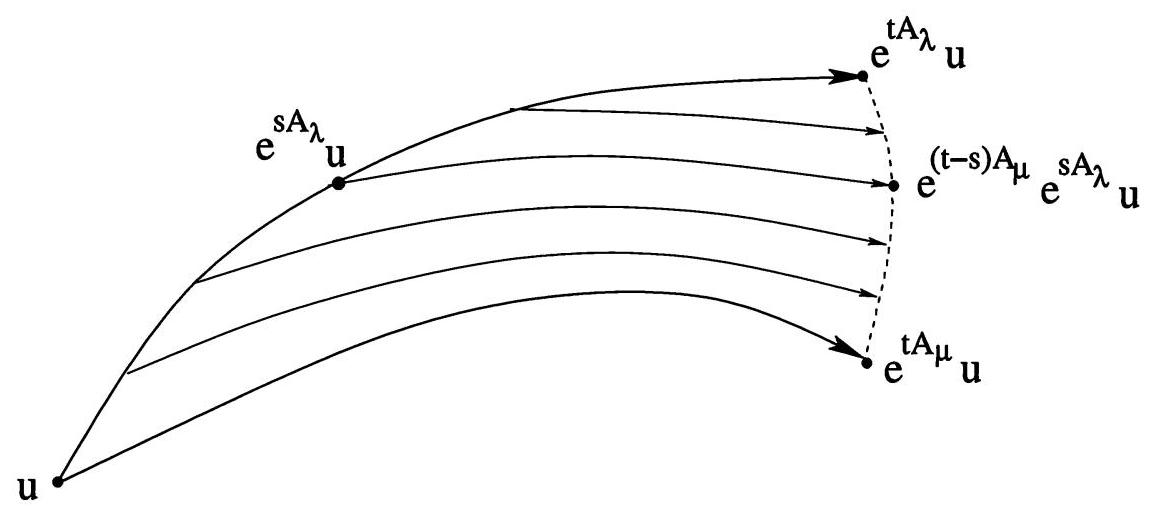
\includegraphics[width=0.75\textwidth]{images/bo_d6ik6nn7aajc739ct1l0_143_164_1407_1153_511_0.jpg}
\captionof{figure}{证明逼近序列 ${e}^{t{A}_{\lambda }}$ 当 $\lambda  \rightarrow  \infty$ 时的收敛性.差值 $\norm{{e}^{t{A}_{\lambda }}u - {e}^{t{A}_{\mu }}u}$ 可通过曲线 $s \mapsto  {e}^{\left( {t - s}\right) {A}_{\mu }}{e}^{s{A}_{\lambda }}u$ 的长度估计，其中 $s \in  \left(  {0,t}\right)$ .}
\label{fig:Alambda-convergence}
\end{figure}

利用三角不等式，我们进一步证明:对任意 $v \in  X$ ，该极限在 $t$ 取遍有界区间时一致成立.

事实上，给定 $\varepsilon  > 0$ ，选取满足 $\| u - v\|  \leq  \varepsilon$ 的 $u \in  \operatorname{Dom}\left( A\right)$ .则
{\setjot[-2]\begin{align*}
    &\quad\limsup_{{\lambda ,\mu  \rightarrow  \infty }}\norm{{e}^{t{A}_{\lambda }}v - {e}^{t{A}_{\mu }}v}\\
    &\leq  \limsup_{{\lambda  \rightarrow  \infty }}\norm{{e}^{t{A}_{\lambda }}v - {e}^{t{A}_{\lambda }}u} + \limsup_{{\lambda ,\mu  \rightarrow  \infty }}\norm{{e}^{t{A}_{\lambda }}u - {e}^{t{A}_{\mu }}u}\\
    &\quad+\limsup_{{\mu  \rightarrow  \infty }}\norm{{e}^{t{A}_{\mu }}u - {e}^{t{A}_{\mu }}v}\\
    &\leq  2\limsup_{{\lambda  \rightarrow  \infty }}\norm{e}^{t{A}_{\lambda }}\norm{v - u} \leq  2{e}^{2\omega t}\varepsilon
\end{align*}}

由于 $\varepsilon  > 0$ 是任意的，故所断言成立.

\noindent 5．由前一步可知，对任意 $t \geq  0$ 与 $u \in  X$ ，下列极限良定义:
\[
{S}_{t}u \doteq  \mathop{\lim }\limits_{{\lambda  \rightarrow  \infty }}{e}^{t{A}_{\lambda }}u
\]

我们断言 $\left\{  {{S}_{t};t \geq  0}\right\}$ 是类型为 $\omega$ 的强连续半群.

事实上，半群性质由下式推出
\[
{S}_{t}{S}_{s}u = \mathop{\lim }\limits_{{\lambda  \rightarrow  \infty }}{e}^{t{A}_{\lambda }}{e}^{s{A}_{\lambda }}u = \mathop{\lim }\limits_{{\lambda  \rightarrow  \infty }}{e}^{\left( {t + s}\right) {A}_{\lambda }}u = {S}_{t + s}u.
\]

对固定 $u \in  X$ ，映射 $t \mapsto  {S}_{t}u$ 连续，因其为连续映射 $t \mapsto  {e}^{t{A}_{\lambda }}u$ 在 $t$ 取遍有界区间时的一致极限.

最后，对任意满足 $\| u\|  \leq  1$ 的 $t \geq  0$ 与 $u \in  X$ ，我们有如下估计
{\setjot[-2]\begin{align*}
\norm{{S}_{t}u} &= \mathop{\lim }\limits_{{\lambda  \rightarrow  \infty }}\norm{{e}^{t{A}_{\lambda }}u} \leq  \limsup_{{\lambda  \rightarrow  \infty }}\norm{e}^{t{A}_{\lambda }}\| u\|\\
&\leq  \mathop{\lim }\limits_{{\lambda  \rightarrow  \infty }}{e}^{{t\lambda \omega }/\left( {\lambda  - \omega }\right) }\| u\|  = {e}^{t\omega }\| u\| .
\end{align*}}

这证明了 $\norm{S}_{t} \leq  {e}^{t\omega }$ ，即该半群为类型 $\omega$ .

\noindent 6．尚需证明线性算子 $A$ 确为该半群的生成元.为此，记 $B$ 为半群 $\left\{  {{S}_{t};t \geq  0}\right\}$ 的生成元.据前述分析，已知 $B$ 是定义在 $\operatorname{Dom}\left( B\right)$ (在 $X$ 中稠密)上的线性闭算子.需证 $B = A$ .

由于 ${A}_{\lambda }$ 是半群 $\left\{  {{e}^{t{A}_{\lambda }};t \geq  0}\right\}$ 的生成元，故对任意 $\lambda  > \omega$ ，有
\begin{equation}\tag{7.34}\label{eq:exp-Alambda-difference}
{e}^{t{A}_{\lambda }}u - u = {\int }_{0}^{t}{e}^{s{A}_{\lambda }}{A}_{\lambda }{u\d s}.
\end{equation}

此外，对 $u \in  \operatorname{Dom}\left( A\right)$ ，三角不等式给出
\begin{equation}\tag{7.35}\label{eq:Alambda-estimate}
\norm{{e}^{s{A}_{\lambda }}{A}_{\lambda }u - {S}_{s}{Au}}  \leq   \norm{e}^{s{A}_{\lambda }}\norm{{A}_{\lambda }u - {Au}} + \norm{{e}^{s{A}_{\lambda }}{Au} - {S}_{s}{Au}}.
\end{equation}

当 $\lambda  \rightarrow  \infty$ 时，\eqref{eq:Alambda-estimate}式右端趋于零，且在 $s$ 取遍有界区间时一致成立.于\eqref{eq:exp-Alambda-difference}式中令 $\lambda  \rightarrow  \infty$ 取极限，即得
\begin{equation}\tag{7.36}\label{eq:semigroup-variation-of-constants-linear}
{S}_{t}u - u = {\int }_{0}^{t}{S}_{s}{Au\d s}\;\forall\,t \geq  0,u \in  \operatorname{Dom}\left( A\right) .
\end{equation}

因此， $\operatorname{Dom}\left( B\right)  \supseteq  \operatorname{Dom}\left( A\right)$ 且
\[
{Bu} = \mathop{\lim }\limits_{{h \rightarrow  0 + }}\frac{{S}_{t}u - u}{t} = \mathop{\lim }\limits_{{t \rightarrow  0 + }}\frac{1}{t}{\int }_{0}^{t}{S}_{s}{Au\d s} = {Au}\;\forall\,u \in  \operatorname{Dom}\left( A\right) .
\]

为证 $A = B$ ，尚需证明 $\operatorname{Dom}\left( B\right)  \subseteq  \operatorname{Dom}\left( A\right)$ .为此，任取 $\lambda  > \omega$ .已知算子
\[
{\lambda I} - A : \operatorname{Dom}\left( A\right)  \mapsto  X\;\text{ and }\;{\lambda I} - B : \operatorname{Dom}\left( B\right)  \mapsto  X
\]
均为单射且满射.特别地， ${\lambda I} - B$ 在 $\operatorname{Dom}\left( A\right)$ 上的限制与 ${\lambda I} - A$ 重合，故为满射.因此，该算子 ${\lambda I} - B$ 无法在保持单射性的前提下延拓至严格大于 $\operatorname{Dom}\left( A\right)$ 的定义域.这表明 $\operatorname{Dom}\left( B\right)  = \operatorname{Dom}\left( A\right)$ ，证毕.
\end{proof}

现考察唯一性.给定一族线性算子半群 $\left\{  {{S}_{t};t \geq  0}\right\}$ ，其生成元由\eqref{eq:generator-def}式中的极限唯一确定.反之，若给定满足定理\ref{thm:hille-yosida}中条件(ii)的线性算子 $A$ ，则我们证明:由 $A$ 生成的半群被唯一确定.

\begin{theorem}[半群的唯一性]\label{thm:semigroup-uniqueness}
设 $\left\{  {S}_{t}\right\}  ,\left\{  {\widetilde{S}}_{t}\right\}$ 为两个强连续线性算子半群，且具有相同的生成元 $A$ .则对每个 $t \geq  0$，均有 ${S}_{t} = {\widetilde{S}}_{t}$ .
\end{theorem}

\begin{proof}
令 $u \in  \operatorname{Dom}\left( A\right)$ .则对每个 $0 \leq  s \leq  t$ ，有 ${\widetilde{S}}_{s}u \in  \operatorname{Dom}\left( A\right)$ 且 ${S}_{t - s}{\widetilde{S}}_{s}u \in  \operatorname{Dom}\left( A\right)$.于是可估计
\[
{\widetilde{S}}_{t}u - {S}_{t}u = {\int }_{0}^{t}\frac{d}{\d s}\left(  {{S}_{t - s}{\widetilde{S}}_{s}u}\right)  {\d s} = {\int }_{0}^{t}\left(  {{S}_{t - s}A{\widetilde{S}}_{s}u - A{S}_{t - s}{\widetilde{S}}_{s}u}\right)  {\d s} = 0.
\]

事实上，
{\setjot[-1]\begin{align*}
    \frac{\d}{\d s}\left(  {{S}_{t - s}{\widetilde{S}}_{s}u}\right)   &= \mathop{\lim }\limits_{{h \rightarrow  0}}\frac{{S}_{t - s - h}\left( {{\widetilde{S}}_{s + h}u}\right)  - {S}_{t - s}{\widetilde{S}}_{s}u}{h}\\
    &= \mathop{\lim }\limits_{{h \rightarrow  0}}\frac{{S}_{t - s - h}\left( {{\widetilde{S}}_{s + h}u - {\widetilde{S}}_{s}u}\right) }{h} + \mathop{\lim }\limits_{{h \rightarrow  0}}\frac{{S}_{t - s - h}\left( {{\widetilde{S}}_{s}u}\right)  - {S}_{t - s}\left( {{\widetilde{S}}_{s}u}\right) }{h}\\
    &= {S}_{t - s}\left( {A{\widetilde{S}}_{s}u}\right)  - A{S}_{t - s}\left( {{\widetilde{S}}_{s}u}\right)  = 0.
\end{align*}}


这表明:对每个固定的 $t \geq  0$ ，有界线性算子 ${S}_{t}$ 与 ${\widetilde{S}}_{t}$ 在稠密子集 $\operatorname{Dom}\left( A\right)$ 上重合.故 ${S}_{t} = {\widetilde{S}}_{t}$ .
\end{proof}

半群理论在演化型偏微分方程求解中的应用将在第9章予以说明.

\section{习题}

\begin{rbhw}[index=1]
假设\eqref{eq:diagonal-operator-l1}式中的算子 $A$ 是扇形的，即对某个 $\omega  \in  \mathbb{R}$ 和某个角 $\overline{\theta } < \pi /2$ ，\eqref{eq:sectorial-eigs}式成立.

(i) 对 $t > 0$ ，给出算子 $\norm{A{e}^{tA}}$ 范数的先验估计，该估计仅依赖于 $\omega ,\overline{\theta }$ .

(ii) 更一般地，对 $t > 0$ 和 $k \geq  1$ ，证明算子 ${A}^{k}{e}^{tA}$ 同样有界，并估计范数 $\norm{{A}^{k}{e}^{tA}}$ .

\end{rbhw}

\begin{rbhw}
设 $A$ 是一个压缩半群的生成元.证明:对每个 $\lambda  > 0$ ，\eqref{eq:Alambda-def}式中的有界线性算子 ${A}_{\lambda }$ 也生成一个压缩半群.

\end{rbhw}

\begin{rbhw}
固定 $\lambda  > 0$ ，并考虑权函数
\[
w\left( t\right)  = \begin{cases} \lambda {e}^{-{\lambda t}} & \text{ if }t \geq  0, \\  0 & \text{ if }t < 0. \end{cases}
\]

对 $n \geq  1$ 归纳，验证 $n$ 重卷积 ${w}_{n} \doteq  w * w * \cdots  * w$ 由下式给出

\begin{equation}\tag{7.37}\label{eq:wn-convolution}
{w}_{n}\left( t\right)  = \begin{cases} \frac{{\lambda }^{n}}{\left( {n - 1}\right) !}{t}^{n - 1}{e}^{-{\lambda t}} & \text{ if }t \geq  0, \\  0 & \text{ if }t < 0. \end{cases}
\end{equation}

证明 $w\left( \cdot \right)$ 是一个概率测度的密度函数，满足
\[
\text{期望} = {\int }_{0}^{\infty }{tw}\left( t\right) {\d t} = \frac{1}{\lambda }
\]
\[
\text{方差} = {\int }_{0}^{\infty }{\left( t - \frac{1}{\lambda }\right) }^{2}w\left( t\right) {\d t} = {\int }_{0}^{\infty }\left( {{t}^{2} - \frac{1}{{\lambda }^{2}}}\right) w\left( t\right) {\d t} = \frac{1}{{\lambda }^{2}}\text{ . }
\]

因此， ${w}_{n}\left( \cdot \right)$ 是一个均值为 $n/\lambda$ 、方差为 $n/{\lambda }^{2}$ 的概率测度的密度函数.

现固定 $T > 0$ ，并令 ${\lambda }_{n} \doteq  n/T$ .对每个 $n \geq  1$ ，定义
\begin{equation}\tag{7.38}\label{eq:Wn-def}
{W}_{n}\left( t\right)  = \left\{  \begin{aligned} \frac{{\left( n/T\right) }^{n}}{\left( {n - 1}\right) !}{t}^{n - 1}{e}^{-\left( {n/T}\right) t} & & \text{ if }t \geq  0, \\  0 & & \text{ if }t < 0. \end{aligned}\right.
\end{equation}

证明图\ref{fig:Wn-weights}中绘制的 ${W}_{n}\left( \cdot \right)$ 是一个均值为 $n/{\lambda }_{n} = T$ 、方差为 $n/{\left( n/T\right) }^{2} = {T}^{2}/n$ 的概率测度的密度函数.特别地，对每个 $\varepsilon  > 0$ ，有
\begin{equation}\tag{7.39}\label{eq:Wn-concentration}
\mathop{\lim }\limits_{{n \rightarrow  \infty }}\left(  {{\int }_{0}^{T - \varepsilon }{W}_{n}\left( t\right) {\d t} + {\int }_{T + \varepsilon }^{\infty }{W}_{n}\left( t\right) {\d t}}\right)   = 0,\;\mathop{\lim }\limits_{{n \rightarrow  \infty }}{\int }_{T - \varepsilon }^{T + \varepsilon }{W}_{n}\left( t\right) {\d t} = 1.
\end{equation}

\begin{figure}[htbp]
\centering
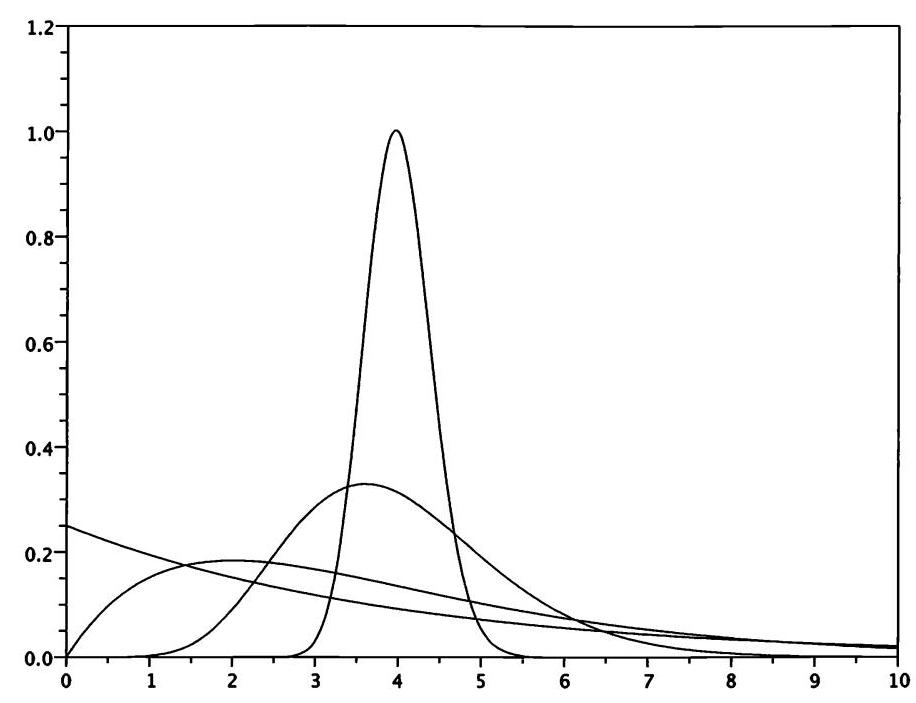
\includegraphics[width=0.8\textwidth]{images/bo_d6ik6nn7aajc739ct1l0_147_261_663_916_703_0.jpg}
\captionof{figure}{由式\eqref{eq:Wn-def}定义的权函数 ${W}_{n}$ 的图像.此处 $T = 4$ ，而 $n = 1,2,{10},{100}$ .所有这些概率分布的平均值均为4，而其方差 $\left( { = {16}/n}\right)$ 随 $n \rightarrow  \infty$ 趋于零.}
\label{fig:Wn-weights}
\end{figure}

\end{rbhw}

\begin{rbhw}
(向后Euler逼近的收敛性)设 $\left\{  {{S}_{t};t \geq  0}\right\}$ 是Banach空间 $X$ 上的一个压缩半群，由线性算子 $A$ 生成.固定 $h > 0$ ，并令 $\lambda  = 1/h$ .对 $n \geq  1$ 进行归纳，将向后Euler逼近公式\eqref{eq:backward-euler-average}推广.即证明
\[
{\left( I - hA\right) }^{-n}u = {\int }_{0}^{\infty }{w}_{n}\left( t\right) {S}_{t}{u\d t}\;\forall\,u \in  X,
\]

其中 ${w}_{n}$ 是式\eqref{eq:wn-convolution}中定义的权函数.

令 $h = T/n$ ，从而 ${\lambda }_{n} = n/T$ .利用\eqref{eq:Wn-concentration}证明:对每个 $u \in  X$ ，有如下收敛性
\[
{\left( I - \frac{T}{n}A\right) }^{-n}u = {\int }_{0}^{\infty }{W}_{n}\left( t\right) {S}_{t}{u\d t} \rightarrow  {S}_{T}u\;\text{ as }n \rightarrow  \infty .
\]

\end{rbhw}

\begin{rbhw}
(正不变集)设 $A$ 是Banach空间 $X$ 上压缩半群 $\left\{  {{S}_{t};t \geq  0}\right\}$ 的生成元.设 $\Omega  \subset  X$ 是一个闭凸子集.证明下列命题等价.

(i) $\Omega$ 是正不变的:若 $u \in  \Omega$ ，则对所有 $t \geq  0$ ，有 ${S}_{t}u \in  \Omega$ .

(ii) $\Omega$ 关于向后Euler算子是不变的:若 $u \in  \Omega$ ，则对每个 $h > 0$ ，均有 ${\left( I - hA\right) }^{-1}u \in  \Omega$ .

\end{rbhw}

\begin{rbhw}
设 $\left\{  {{S}_{t};t \geq  0}\right\}$ 是$\omega$类半群，其生成元为 $A$ .证明:对每个 $\gamma  \in  \mathbb{R}$ ，有界线性算子族 $\left\{  {{e}^{\gamma t}{S}_{t};t \geq  0}\right\}$ 构成一个类型为 $\omega  + \gamma$ 的半群，其生成元为 $A + {\gamma I}$ .

\end{rbhw}

\begin{rbhw}
在空间 ${L}^{p}\left( \mathbb{R}\right)$ 上，考虑由下式定义的线性算子 ${S}_{t}$
\[
\left( {{S}_{t}f}\right) \left( x\right)  = {e}^{-{2t}}f\left( {x + t}\right) .
\]

(i) 证明:线性算子族 $\left\{  {{S}_{t};t \geq  0}\right\}$ 对所有 $1 \leq  p < \infty$ 均构成 ${L}^{p}\left( \mathbb{R}\right)$ 上强连续、压缩的半群.求出该半群的生成元 $A$ . $\operatorname{Dom}\left( A\right)$ 是什么？

(ii) 证明算子族 $\left\{  {{S}_{t};t \geq  0}\right\}$ 在 ${L}^{\infty }\left( \mathbb{R}\right)$ 上 NOT 构成强连续半群.

\end{rbhw}

\begin{rbhw}
设 $\left\{  {{S}_{t};t \geq  0}\right\}$ 是 ${\mathbb{R}}^{n}$ 上的强连续线性算子半群.证明存在一个 $n \times  n$ 矩阵 $A$ ，使得对每个 $t \geq  0$ ，均有 ${S}_{t} = {e}^{tA}$ .

\end{rbhw}

\begin{rbhw}
(半线性方程)设 $A$ 是Banach空间 $X$ 上的线性算子，生成压缩半群 $\left\{  {{S}_{t};t \geq  0}\right\}$.称映射 $u : \left(  {0,T}\right)   \mapsto  X$ 为半线性Cauchy问题的温和解
\begin{equation}\tag{7.40}\label{eq:semilinear-cauchy-problem}
\frac{d}{\d t}u\left( t\right)  = {Au}\left( t\right)  + f\left( {t,u\left( t\right) }\right) ,\;u\left( 0\right)  = \bar{u}
\end{equation}
如果
\begin{equation}\tag{7.41}\label{eq:mild-solution}
u\left( t\right)  = {S}_{t}\bar{u} + {\int }_{0}^{t}{S}_{t - s}f\left( {s,u\left( s\right) }\right) {\d s}\;\forall\,t \in  \left(  {0,T}\right)  .
\end{equation}

(i) 假设 $f : \left(  {0,T}\right)   \times  X \mapsto  X$ 连续且满足如下估计式
\[
\| f\left( {t,x}\right) \|  \leq  M,\;\| f\left( {t,x}\right)  - f\left( {t,y}\right) \|  \leq  L\| x - y\| \;\forall\,t,x,y,
\]

证明Cauchy问题\eqref{eq:semilinear-cauchy-problem}存在唯一温和解.

(ii) 在 $A$ 为有界算子的特殊情形下，即 ${S}_{t} = {e}^{tA}$ 成立，证明 $u\left( \cdot \right)$ 满足\eqref{eq:mild-solution}当且仅当 $u$ 是Cauchy问题\eqref{eq:semilinear-cauchy-problem}的连续可微解.

\end{rbhw}

\begin{rbhw}
固定时间 $T > 0$ .在空间 $X = {L}^{1}\left( \left(  {0,1}\right)  \right)$ 上，构造一个强连续的压缩线性算子半群 $\left\{  {{S}_{t};t \geq  0}\right\}$ ，使得对 $0 \leq  t < T$ 有 $\norm{S}_{t} = 1$ ，但对 $t \geq  T$ 有 $\norm{S}_{t} = 0$ .

\end{rbhw}

\begin{rbhw}
设 $\left\{  {{S}_{t};t \geq  0}\right\}$ 是Banach空间 $X$ 上的强连续压缩线性算子半群.假设对给定时间 $\tau  > 0$ ，算子 ${S}_{\tau }$ 是紧的.证明:对任意 $t > \tau$ ，算子 ${S}_{t}$ 也是紧的.构造一个反例，说明当 $0 \leq \; t < \tau$ 时，算子 ${S}_{t}$ 未必是紧的.

\end{rbhw}

\begin{rbhw}
在空间 ${L}^{1}\left( \mathbb{R}\right)$ 上，考虑定义域为 ${Au} = \frac{\partial }{\partial x}u$ 的算子

$\operatorname{Dom}\left( A\right)  = \left\{  {u \in  {L}^{1}\left( \mathbb{R}\right) ;u\text{ is absolutely continuous, }{u}_{x} \in  {L}^{1}\left( \mathbb{R}\right) }\right\}$ .

(i) 描述由 $A$ 生成的半群 $\left\{  {{S}_{t};t \geq  0}\right\}$ .

(ii) 对任意 $u \in  {L}^{1}\left( \mathbb{R}\right)$ 与 $h > 0$ ，构造后向Euler逼近 ${E}_{h}^{ - }u$ .

(iii) 设 $u \in  {\mathcal{C}}_{c}^{\infty }\left( \mathbb{R}\right)$ 是具有紧支集的光滑函数，例如满足当 $x \notin  \left(  {a,b}\right)$ 时 $u\left( x\right)  = 0$ .对任意时间步长 $h > 0$ ，证明前向Euler逼近 ${\left( {E}_{h}^{ + }\right) }^{n}u = {\left( I + hA\right) }^{n}u$ 良定义，且其支集包含于 $\left(  {a,b}\right)$ .

(iv) 利用(iii)，证明:对每个足够大的时间 $\tau  > 0$ ，函数 ${\left( I + \frac{\tau }{n}A\right) }^{n}u$ 不能随 $n \rightarrow  \infty$ 趋于 ${S}_{\tau }u$ .

\end{rbhw}


\chapter{Soblev空间}\vspace{-2em}

本章介绍Soblev空间的基本理论；该理论为线性及非线性偏微分方程的分析提供了极为有用的抽象框架.我们首先引入分布理论，并给出若干启发性例子.

\section{分布与弱导数}

以下， ${L}_{\text{ loc }}^{1}\left( \mathbb{R}\right)$ 表示局部可积函数空间 $f : \mathbb{R} \mapsto  \mathbb{R}$ .这些是Lebesgue可测函数，且在每个有界区间上可积.
\begin{definition}[支集]
    函数 $\phi$ 的\colorbf{支集}是集合 $\{ x;\phi \left( x\right)  \neq  0\}$ 的闭包，其中 $\phi$ 不为零，记为$\operatorname{Supp}\left( \phi \right)$.
\end{definition}
 ${\mathcal{C}}_{c}^{\infty }\left( \mathbb{R}\right)$ 表示具有紧支集的连续函数空间，且具有任意阶连续导数.

每个局部可积函数 $f \in  {L}_{\text{ loc }}^{1}\left( \mathbb{R}\right)$ 确定一个线性泛函 ${\Lambda }_{f} : {\mathcal{C}}_{c}^{\infty }\left( \mathbb{R}\right)  \mapsto  \mathbb{R}$ ，即
\begin{equation}\tag{8.1}\label{eq:distribution-functional}
{\Lambda }_{f}\left( \phi \right)  \doteq  {\int }_{\mathbb{R}}f\left( x\right) \phi \left( x\right) {\d x}.
\end{equation}

注意，该积分对每个 $\phi  \in  {\mathcal{C}}_{c}^{\infty }\left( \mathbb{R}\right)$ 均有定义.此外，若 Supp $\left( \phi \right)  \subseteq  \left(  {a,b}\right)$ ，则有如下估计
\begin{equation}\tag{8.2}\label{eq:distribution-functional-bound}
\left| {{\Lambda }_{f}\left( \phi \right) }\right|  \leq  \left( {{\int }_{a}^{b}\left| {f\left( x\right) }\right| {\d x}}\right) \| \phi {\| }_{{\mathcal{C}}^{0}}.
\end{equation}

接下来，假设 $f$ 连续可微.则其导数
\[
{f}^{\prime }\left( x\right)  = \mathop{\lim }\limits_{{h \rightarrow  0}}\frac{f\left( {x + h}\right)  - f\left( x\right) }{h}
\]
连续，因而局部可积.相应地， ${f}^{\prime }$ 也在 ${\mathcal{C}}_{c}^{\infty }\left( \mathbb{R}\right)$ 上确定一个线性泛函，即
\begin{equation}\tag{8.3}\label{eq:distribution-derivative-by-parts}
{\Lambda }_{{f}^{\prime }}\left( \phi \right)  \doteq  {\int }_{\mathbb{R}}{f}^{\prime }\left( x\right) \phi \left( x\right) {\d x} =  - {\int }_{\mathbb{R}}f\left( x\right) {\phi }^{\prime }\left( x\right) {\d x}.
\end{equation}

此时，一个关键观察是:式\eqref{eq:distribution-derivative-by-parts}中第一个积分仅当 ${f}^{\prime }\left( x\right)$ 在几乎处处 $x$ 处存在且局部可积时才有定义.然而，第二个积分对任一局部可积函数 $f$ 均有定义，即使 $f$ 在任何点处都不存在点态导数。此外，若 $\operatorname{Supp}\left( \phi \right)  \subseteq  \left(  {a,b}\right)$ ，则有如下估计
\[
\left| {{\Lambda }_{{f}^{\prime }}\left( \phi \right) }\right|  \leq  \left( {{\int }_{a}^{b}\left| {f\left( x\right) }\right| {\d x}}\right) \| \phi {\| }_{{\mathcal{C}}^{1}}.
\]

该构造亦可推广至高阶导数.

\begin{definition}[分布导数与弱导数]\label{def:distribution-derivative}
给定整数 $k \geq  1$ ， $f \in  {L}_{\text{ loc }}^{1}\left( \mathbb{R}\right)$ 的$k$阶分布导数是指线性泛函
\[
{\Lambda }_{{D}^{k}f}\left( \phi \right)  \doteq  {\left( -1\right) }^{k}{\int }_{\mathbb{R}}f\left( x\right) {D}^{k}\phi \left( x\right) {\d x}.
\]

若存在局部可积函数 $g$ ，使得 ${\Lambda }_{g} = {\Lambda }_{{D}^{k}f}$ ，即
\[
{\int }_{\mathbb{R}}g\left( x\right) \phi \left( x\right) {\d x} = {\left( -1\right) }^{k}{\int }_{\mathbb{R}}f\left( x\right) {D}^{k}\phi \left( x\right) {\d x}\;\forall\,\phi  \in  {\mathcal{C}}_{c}^{\infty }\left( \mathbb{R}\right) ,
\]

则称 $g$ 是 $f$ 的$k$阶的\colorbf{弱导数}.
\end{definition}

\begin{remark}\label{rem:weak-derivative-nullset}
经典导数以差商极限形式逐点定义；而弱导数仅以积分意义定义，且在零测集上可任意修改.在零测集上任意改变函数 $f$ ，不会以任何方式影响其弱导数.
\end{remark}

\begin{instance}\label{ins:weak-derivative-ramp}
考虑函数
\[
f\left( x\right)  \doteq  \left\{  \begin{array}{ll} 0 & \text{ if }x \leq  0, \\  x & \text{ if }x > 0. \end{array}\right.
\]

其分布导数为映射
\[
\Lambda \left( \phi \right)  =  - {\int }_{0}^{\infty }x \cdot  {\phi }^{\prime }\left( x\right) {\d x} = {\int }_{\mathbb{R}}H\left( x\right) \phi \left( x\right) {\d x},
\]

其中
\begin{equation}\tag{8.4}\label{eq:heaviside}
H\left( x\right)  = \left\{  \begin{array}{ll} 0 & \text{ if }x \leq  0 \\  1 & \text{ if }x > 0 \end{array}\right.
\end{equation}

本例中，式\eqref{eq:heaviside}中的 Heaviside 函数 $H$ 即为 $f$ 的弱导数.
\end{instance}

\begin{instance}\label{ins:heaviside-dirac}
式\eqref{eq:heaviside}中的函数 $H$ 局部可积.其分布导数为线性泛函
\[
\Lambda \left( \phi \right)  \doteq   - {\int }_{\mathbb{R}}H\left( x\right) {\phi }^{\prime }\left( x\right) {\d x} =  - {\int }_{0}^{\infty }{\phi }^{\prime }\left( x\right) {\d x} = \phi \left( 0\right) .
\]

这对应于 Dirac 测度，将单位质量集中于原点.我们断言函数 $H$ 不存在弱导数，即不存在任何局部可积函数 $g$ ，使得
\begin{equation}\tag{8.5}\label{eq:dirac-functional}
\int g\left( x\right) \phi \left( x\right) {\d x} = \phi \left( 0\right) \;\forall\,\phi  \in  {\mathcal{C}}_{c}^{\infty }.
\end{equation}

事实上，若\eqref{eq:dirac-functional}成立，则由 Lebesgue 控制收敛定理
\[
\mathop{\lim }\limits_{{h \rightarrow  0}}{\int }_{-h}^{h}\left| {g\left( x\right) }\right| {\d x} = 0
\]

因此可选取 $\delta  > 0$ 使得 ${\int }_{-\delta }^{\delta }\left| {g\left( x\right) }\right| {\d x} \leq  1/2$ .令 $\phi  : \mathbb{R} \mapsto  \left(  {0,1}\right)$ 为一光滑函数，满足 $\phi \left( 0\right)  = 1$ ，且其支集包含于区间 $\left(  {-\delta ,\delta }\right)$ 内.现通过下式导出矛盾
{\begin{align*}
1 = \phi \left( 0\right)  = \Lambda \left( \phi \right)  &= {\int }_{\mathbb{R}}g\left( x\right) \phi \left( x\right) {\d x} = {\int }_{-\delta }^{\delta }g\left( x\right) \phi \left( x\right) {\d x}\\
&\leq  \mathop{\max }\limits_{x}\left| {\phi \left( x\right) }\right|  \cdot  {\int }_{-\delta }^{\delta }\left| {g\left( x\right) }\right| {\d x} \leq  \frac{1}{2}.
\end{align*}}
\end{instance}

\begin{instance}\label{ins:rational-irrational-weak-derivative}
考虑函数
\[
f\left( x\right)  \doteq  \begin{cases} 0 & x\in \mathbb{Q} \\  2 + \sin x & x\in\mathbb{R}\setminus\mathbb{Q}\end{cases}
\]

该函数 $f$ 在每一点均不连续，故处处不可微.另一方面，函数 $g\left( x\right)  = \cos x$ 为 $f$ 提供了弱导数.事实上， $f$ 在有理点集(测度为零)上的行为无关紧要.于是我们有
\[
- \int f\left( x\right) {\phi }^{\prime }\left( x\right) {\d x} =  - \int \left( {2 + \sin x}\right) {\phi }^{\prime }\left( x\right) {\d x} = \int \left( {\cos x}\right) \phi \left( x\right) {\d x}.
\]
\end{instance}

\begin{instance}\label{ins:cantor-no-weak-derivative}
考虑 Cantor 函数 $f : \mathbb{R} \mapsto  \left(  {0,1}\right)$ ，其定义为
\begin{equation}\tag{8.6}\label{eq:cantor-function}
f\left( x\right) =\begin{cases} 0 &x \leq  0, \\  
    1 &x \geq  1, \\  
    1/2 &x \in  \left(  {1/3,2/3}\right)  , \\  
    1/4 &x \in  \left(  {1/9,2/9}\right)  , \\  
    3/4 &x \in  \left(  {7/9,8/9}\right)  , \\   
    \quad\quad\quad\ldots &  \end{cases}
\end{equation}

(见图\ref{fig:cantor-function-test}).这是一个连续但非绝对连续函数的标准例子.我们断言 $f$ 不存在弱导数.事实上，假设相反地 $g \in  {L}_{\text{ loc }}^{1}$ 是 $f$ 的弱导数.由于 $f$ 在每个开集

\[
(-\infty ,0),(1, + \infty) ,\left(\frac{1}{3},\frac{2}{3}\right),\left(\frac{1}{9},\frac{2}{9}\right),\left(\frac{7}{9},\frac{8}{9}\right),\ldots
\]

\begin{figure}[htbp]
\centering
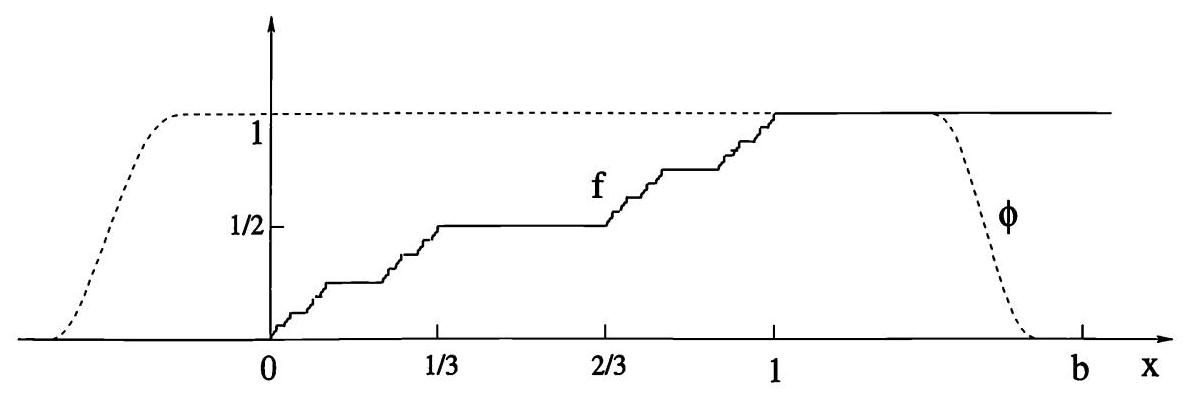
\includegraphics[width=0.9\textwidth]{images/bo_d6ik6nn7aajc739ct1l0_154_150_227_1183_394_0.jpg}
\caption{Cantor函数 $f$ 及一个检验函数 $\phi$ ，表明 $g\left( x\right)  \equiv  0$ 不可能是 $f$ 的弱导数.}
\label{fig:cantor-function-test}
\end{figure}
\noindent 上为常数，故 $g\left( x\right)  = {f}^{\prime }\left( x\right)  = 0$ 必在这些开区间的并集上为零.因此对几乎处处的 $x \in  \mathbb{R}$ ，有 $g\left( x\right)  = 0$ .为导出矛盾，需证明函数 $g \equiv  0$ 并非 $f$ 的弱导数.如图\ref{fig:cantor-function-test}所示，取检验函数 $\phi  \in  {\mathcal{C}}_{c}^{\infty }$ ，使得当 $x \in  \left(  {0,1}\right)$ 时 $\phi \left( x\right)  = 1$ ，而当 $x \geq  b$ 时 $\phi \left( x\right)  = 0$ .则
\[
\int g\left( x\right) \phi \left( x\right) {\d x} = 0 \neq  1 =  - \int f\left( x\right) {\phi }^{\prime }\left( x\right) {\d x}.
\]
\end{instance}

\subsection{分布}
前一节所述构造可推广至多维空间中任意开区域.设 $\Omega  \subseteq  {\mathbb{R}}^{n}$ 为一开集.记 ${L}_{\text{ loc }}^{1}\left( \Omega \right)$ 为 $\Omega$ 上局部可积函数的空间.这些是可测函数 $f : \Omega  \mapsto  \mathbb{R}$ ，其在每个紧子集 $K \subset  \Omega$ 上的限制均可积.

\begin{instance}\label{ins:L1loc-examples}
函数 ${e}^{x}$ 与 $\ln \left| x\right|$ 属于 ${L}_{\text{ loc }}^{1}\left( \mathbb{R}\right)$ ，而 ${x}^{-1} \notin \; {L}_{\text{ loc }}^{1}\left( \mathbb{R}\right)$ .另一方面，函数 $f\left( x\right)  = {x}^{\gamma }$ 对任意(正或负)指数 $\gamma  \in  \mathbb{R}$ 均属于 ${L}_{\text{ loc }}^{1}\left(  \right)  0,\infty \left(  \right)$ .在多个空间维数下，若 $\gamma  < n$ ，则函数 $f\left( x\right)  = {\left| x\right| }^{-\gamma }$ 属于 ${L}_{\text{ loc }}^{1}\left( {\mathbb{R}}^{n}\right)$ .需谨记:函数 $f \in  {L}_{\text{ loc }}^{1}$ 在零测集上的逐点取值无关紧要.
\end{instance}

我们用 ${\mathcal{C}}_{\mathrm{c}}^{\infty }\left( \Omega \right)$ 表示所有阶连续偏导数均存在且连续、支集为 $\Omega$ 的紧子集的连续函数 $\phi  : \Omega  \mapsto  \mathbb{R}$ 所构成的空间.函数 $\phi  \in  {\mathcal{C}}_{\mathrm{c}}^{\infty }\left( \Omega \right)$ 通常称为“检验函数”.我们回顾:函数 $\phi$ 的支集是 $\phi$ 不为零之处的集合的闭包:
\[
\operatorname{Supp}\left( \phi \right)  \doteq  \overline{\{ x \in  \Omega ;\phi \left( x\right)  \neq  0\} }.
\]

我们需要一种高效方式来表示函数 $f$ 的高阶导数.多重指标 $\alpha  = \left( {{\alpha }_{1},{\alpha }_{2},\ldots ,{\alpha }_{n}}\right)$ 是一个由非负整数构成的 $n$ 元组.其长度定义为
\[
\left| \alpha \right|  \doteq  {\alpha }_{1} + {\alpha }_{2} + \cdots  + {\alpha }_{n}.
\]

每个多重指标 $\alpha$ 确定一个阶数为 $\left| \alpha \right|$ 的偏微分算子，即
\[
{D}^{\alpha }f = {\left( \frac{\partial }{\partial {x}_{1}}\right) }^{{\alpha }_{1}}{\left( \frac{\partial }{\partial {x}_{2}}\right) }^{{\alpha }_{2}}\cdots {\left( \frac{\partial }{\partial {x}_{n}}\right) }^{{\alpha }_{n}}f.
\]

\begin{definition}[分布]\label{def:distribution}
开集 $\Omega  \subseteq  {\mathbb{R}}^{n}$ 上的\colorbf{分布}是一个线性泛函 $\Lambda  : {\mathcal{C}}_{c}^{\infty }\left( \Omega \right)  \mapsto  \mathbb{R}$ ，满足如下有界性条件:对每个紧集 $K \subset  \Omega$ ，存在整数 $N \geq  0$ 和常数 $C$ ，使得
\begin{equation}\tag{8.7}\label{eq:distribution-bound}
\left| {\Lambda \left( \phi \right) }\right| \; \leq  \;C\| \phi {\| }_{{\mathcal{C}}^{N}},\;\forall\,\phi  \in  {\mathcal{C}}^{\infty }\,\text{满足}\,\mathrm{{Supp}}\left( \phi \right)  \subseteq  K\;.
\end{equation}
\end{definition}

换言之，对所有在给定紧集 $K$ 外消失的检验函数 $\phi$ ，其值 $\Lambda \left( \phi \right)$ 应以 $\phi$ 的各阶导数(至某阶 $N$ 为止)的最大值为界.

注意，此处 $N$ 与 $C$ 均依赖于紧子集 $K$ .若存在一个与 $K$ 无关的整数 $N \geq  0$ ，使得\eqref{eq:distribution-bound}式成立(其中 $C = \; {C}_{K}$ 仍可依赖于 $K$ )，则称该分布具有有限阶.满足此条件的最小整数 $N$ 称为该分布的阶.

\begin{instance}\label{ins:Lf-is-distribution}
设 $\Omega$ 为 ${\mathbb{R}}^{n}$ 的一个开子集，并考虑函数 $f \in  {L}_{\mathrm{{loc}}c}^{1}\left( \Omega \right)$ .则由下式定义的线性映射 ${\Lambda }_{f} : {\mathcal{C}}_{c}^{\infty }\left( \Omega \right)  \mapsto  \mathbb{R}$
\begin{equation}\tag{8.8}\label{eq:Lf-definition}
{\Lambda }_{f}\left( \phi \right)  \doteq  {\int }_{\Omega }{f\phi \d x}
\end{equation}
是一种分布.事实上，显然 ${\Lambda }_{f}$ 是良定义的且是线性的.对任意紧子集 $K \subset  \Omega$ ，每个支集满足 $\operatorname{Supp}\left( \phi \right)  \subseteq  K$ 的检验函数 $\phi$ 均满足如下估计
\[
\left| {{\Lambda }_{f}\left( \phi \right) }\right| \; = \;\left| {{\int }_{K}f\;\phi \;{\d x}}\right| \; \leq  \;{\int }_{K}\left| {f\left( x\right) }\right| \;{\d x} \cdot  \mathop{\max }\limits_{{x \in  K}}\left| {\phi \left( x\right) }\right| \; \leq  \;C\;\| \phi {\| }_{{\mathcal{C}}^{0}}\;.
\]

因此，界\eqref{eq:distribution-bound}在 $C = {\int }_{K}\left| f\right| {\d x}$ 和 $N = 0$ 下成立.这给出了一个零阶分布的例子.
\end{instance}

所有定义在 $\Omega$ 上的分布构成的族显然构成一个向量空间.一个值得注意的事实是:尽管函数 $f$ 可能(在经典意义下)不存在任何偏导数，但对于任一分布 $\Lambda$ ，总可适当地定义其导数.

\begin{definition}[分布的导数]\label{def:distribution-derivative}
给定一分布 $\Lambda$ 及一多重指标 $\alpha$ ，我们通过下式定义分布 ${D}^{\alpha }\Lambda$
\begin{equation}\tag{8.9}\label{eq:distribution-derivative}
{D}^{\alpha }\Lambda \left( \phi \right)  \doteq  {\left( -1\right) }^{\left| \alpha \right| }\Lambda \left( {{D}^{\alpha }\phi }\right) .
\end{equation}
\end{definition}

易验证 ${D}^{\alpha }\Lambda$ 本身亦为一分布.事实上，映射 $\phi  \mapsto  {D}^{\alpha }\Lambda \left( \phi \right)$ 的线性性是显然的.其次，设 $K$ 是 $\Omega$ 的一个紧子集，且设 $\phi$ 是支集包含于 $K$ 的检验函数.由假设，存在常数 $C$ 和整数 $N \geq  0$ ，使得\eqref{eq:distribution-bound}成立.由此可得
\[
\left| {{D}^{\alpha }\Lambda \left( \phi \right) }\right|  = \left| {\Lambda \left( {{D}^{\alpha }\phi }\right) }\right|  \leq  C{\norm{D}^{\alpha }\phi }_{{\mathcal{C}}^{N}} \leq  C\| \phi {\| }_{{\mathcal{C}}^{N + \left| \alpha \right| }}.
\]

故 ${D}^{\alpha }\Lambda$ 亦满足\eqref{eq:distribution-bound}，其中 $N$ 被替换为 $N + \left| \alpha \right|$ .

注意，若 ${\Lambda }_{f}$ 是\eqref{eq:Lf-definition}中对应于函数 $f$ 的分布，且该函数 $f$ 是 $\left| \alpha \right|$ 次连续可微的，则可通过分部积分得到
{\setjot[-2]\begin{align*}
    {D}^{\alpha }{\Lambda }_{f}\left( \phi \right)  &= {\left( -1\right) }^{\left| \alpha \right| }{\Lambda }_{f}\left( {{D}^{\alpha }\phi }\right)  = {\left( -1\right) }^{\left| \alpha \right| }\int f\left( x\right) {D}^{\alpha }\phi \left( x\right) {\d x}\\
    &= \int {D}^{\alpha }f\left( x\right) \phi \left( x\right) {\d x} = {\Lambda }_{{D}^{\alpha }f}\left( \phi \right) .
\end{align*}}
这证明了公式\eqref{eq:distribution-derivative}的合理性.

\subsection{弱导数}
对每个局部可积函数 $f$ 及每个多重指标 $\alpha  = \left( {{\alpha }_{1},\ldots ,{\alpha }_{n}}\right)$ ，分布 ${\Lambda }_{f}$ 总存在按\eqref{eq:distribution-derivative}定义的分布意义下的导数 ${D}^{\alpha }{\Lambda }_{f}$ .在某些情形下，可找到一个局部可积函数 $g$ ，使得分布 ${D}^{\alpha }{\Lambda }_{f}$ 恰好等于由 ${\Lambda }_{g}$ 所确定的分布.这便引出了弱导数的概念.

\begin{definition}[弱导数]\label{def:weak-derivative}
设 $f \in  {L}_{\text{ loc }}^{1}\left( \Omega \right)$ 是开集 $\Omega  \subseteq  {\mathbb{R}}^{n}$ 上的局部可积函数， ${\Lambda }_{f}$ 是其对应的分布(如\eqref{eq:Lf-definition}所定义).给定一多重指标 $\alpha  = \left( {{\alpha }_{1},\ldots ,{\alpha }_{n}}\right)$ ，若存在局部可积函数 $g \in  {L}_{\text{ loc }}^{1}\left( \Omega \right)$ ，使得 ${D}^{\alpha }{\Lambda }_{f} = {\Lambda }_{g}$ ，即
\begin{equation}\tag{8.10}\label{eq:weak-derivative}
\int f{D}^{\alpha }{\phi \d x} = {\left( -1\right) }^{\left| \alpha \right| }\int {g\phi \d x},\;\forall\,\text{测试函数}\,\phi  \in  {\mathcal{C}}_{\mathrm{c}}^{\infty }\left( \Omega \right) ,
\end{equation}
则称 $g$ 是 $f$ 的\colorbf{弱 $\alpha$ 阶导数}，并记作 $g = {D}^{\alpha }f$ .
\end{definition}

一般而言，弱导数未必存在.特别地，例\ref{ins:heaviside-dirac}表明，Heaviside 函数不具有弱导数.事实上，其分布意义下的导数是一个 Dirac 测度(在原点处集中单位质量)，而非局部可积函数.另一方面，若弱导数存在，则它在几乎处处意义下是唯一的.

\begin{lemma}[弱导数的唯一性]\label{lem:weak-derivative-uniqueness}
设 $f \in  {L}_{\text{ loc }}^{1}\left( \Omega \right)$ ，且 $g,\widetilde{g} \in  {L}_{\text{ loc }}^{1}\left( \Omega \right)$ 是 $f$ 的弱 $\alpha$ 阶导数，即
\[
\int f{D}^{\alpha }{\phi \d x} = {\left( -1\right) }^{\left| \alpha \right| }\int {g\phi \d x} = {\left( -1\right) }^{\left| \alpha \right| }\int \widetilde{g}{\phi \d x}
\]
对所有检验函数 $\phi  \in  {\mathcal{C}}_{\mathrm{c}}^{\infty }\left( \Omega \right)$ 成立.则 $g\left( x\right)  = \widetilde{g}\left( x\right)$ 几乎处处成立于 $x \in  \Omega$ .
\end{lemma}

\begin{proof}
由假设，函数 $\left( {g - \widetilde{g}}\right)  \in  {L}_{\text{ loc }}^{1}\left( \Omega \right)$ 满足
\[
\int \left( {g - \widetilde{g}}\right) {\phi \d x} = 0,\;\forall\,\text{测试函数}\,\phi  \in  {\mathcal{C}}_{\mathrm{c}}^{\infty }\left( \Omega \right) .
\]

因此，由附录中推论A.17可得 $g\left( x\right)  - \widetilde{g}\left( x\right)  = 0$几乎处处成立于 $x \in  \Omega$ .
\end{proof}

若函数 $f$ 二阶连续可微，则微积分基本定理指出:偏导数可交换顺序，即 ${f}_{{x}_{j}{x}_{k}} = {f}_{{x}_{k}{x}_{j}}$ .该性质对弱导数仍成立.为一般性地陈述此结果，我们回顾:两个多重指标 $\alpha  = \left( {{\alpha }_{1},\ldots ,{\alpha }_{n}}\right)$ 与 $\beta  = \left( {{\beta }_{1},\ldots ,{\beta }_{n}}\right)$ 的和定义为 $\alpha  + \beta  = \left( {{\alpha }_{1} + {\beta }_{1},\ldots ,{\alpha }_{n} + {\beta }_{n}}\right)$ .

\begin{lemma}[弱导数可交换]\label{lem:weak-derivative-commute}
设 $f \in  {L}_{\text{ loc }}^{1}\left( \Omega \right)$ 对每个 $\left| \alpha \right|  \leq  k$ 均存在弱导数 ${D}^{\alpha }f$ .则对任意满足 $\left| \alpha \right|  + \left| \beta \right|  \leq  k$ 的多重指标对 $\alpha ,\beta$ ，有
\begin{equation}\tag{8.11}\label{eq:weak-derivative-commute}
{D}^{\alpha }\left( {{D}^{\beta }f}\right)  = {D}^{\beta }\left( {{D}^{\alpha }f}\right)  = {D}^{\alpha  + \beta }f.
\end{equation}
\end{lemma}

\begin{proof}
考虑任意检验函数 $\phi  \in  {\mathcal{C}}_{c}^{\infty }\left( \Omega \right)$ .利用 ${D}^{\beta }\phi  \in \; {\mathcal{C}}_{\mathrm{c}}^{\infty }\left( \Omega \right)$ 同样是检验函数，可得
{\setjot[-2]\begin{align*}
    {\int }_{\Omega }{D}^{\alpha }f{D}^{\beta }{\phi \d x} &= {\left( -1\right) }^{\left| \alpha \right| }{\int }_{\Omega }f\left( {{D}^{\alpha  + \beta }\phi }\right) {\d x}\\
    &= {\left( -1\right) }^{\left| \alpha \right| }{\left( -1\right) }^{\left| \alpha  + \beta \right| }{\int }_{\Omega }\left( {{D}^{\alpha  + \beta }f}\right) {\phi \d x}\\
    &= {\left( -1\right) }^{\left| \beta \right| }{\int }_{\Omega }\left( {{D}^{\alpha  + \beta }f}\right) {\phi \d x}.
\end{align*}}



由定义，这意味着 ${D}^{\alpha  + \beta }f = {D}^{\beta }\left( {{D}^{\alpha }f}\right)$ .在前述计算中交换多重指标 $\alpha$ 与 $\beta$ 的角色，可得 ${D}^{\alpha  + \beta }f = \; {D}^{\alpha }\left( {{D}^{\beta }f}\right)$ .
\end{proof}

下一个引理推广了另一熟知结论:极限的弱导数等于弱导数的极限.

\begin{lemma}[弱导数的收敛性]\label{lem:weak-derivative-convergence}
考虑函数列 ${f}_{n} \in  {L}_{\text{ loc }}^{1}\left( \Omega \right)$ .对固定多重指标 $\alpha$ ，假设每个 ${f}_{n}$ 均存在弱导数 ${g}_{n} = {D}^{\alpha }{f}_{n}$ .若 ${f}_{n} \rightarrow  f$ 且 ${g}_{n} \rightarrow  g$ 在 ${L}_{\text{ loc }}^{1}\left( \Omega \right)$ 中成立，则 $g = {D}^{\alpha }f$ .
\end{lemma}

\begin{proof}
对任一检验函数 $\phi  \in  {\mathcal{C}}_{\mathrm{c}}^{\infty }\left( \Omega \right)$ ，直接计算可得
{\begin{align*}
    {\int }_{\Omega }{g\phi \d x} &= \mathop{\lim }\limits_{{n \rightarrow  \infty }}{\int }_{\Omega }{g}_{n}{\phi \d x} = \mathop{\lim }\limits_{{n \rightarrow  \infty }}{\left( -1\right) }^{\left| \alpha \right| }{\int }_{\Omega }{f}_{n}{D}^{\alpha }{\phi \d x}\\
    &= {\left( -1\right) }^{\left| \alpha \right| }{\int }_{\Omega }f{D}^{\alpha }{\phi \d x}
\end{align*}}
根据定义，这意味着 $g$ 是 $f$ 的 $\alpha$ 阶弱导数.
\end{proof}

\section{磨光化}

如常，设 $\Omega  \subseteq  {\mathbb{R}}^{n}$ 为开集.对给定的 $\varepsilon  > 0$ ，定义开子集
\begin{equation}\tag{8.12}\label{eq:omega-epsilon}
{\Omega }_{\varepsilon } \doteq  \left\{  {x \in  {\mathbb{R}}^{n};\bar{B}\left( {x,\varepsilon }\right)  \subset  \Omega }\right\}  .
\end{equation}

对每个 $u \in  {L}_{\text{ loc }}^{1}\left( \Omega \right)$ ，磨光化
\[
{u}_{\varepsilon }\left( x\right)  \doteq  \left( {{J}_{\varepsilon } * u}\right) \left( x\right)  = {\int }_{B\left( {x,\varepsilon }\right) }{J}_{\varepsilon }\left( {x - y}\right) u\left( y\right) {\d y}
\]
对每个 $x \in  {\Omega }_{\varepsilon }$ 均有定义.此外， ${u}_{\varepsilon } \in  {\mathcal{C}}^{\infty }\left( {\Omega }_{\varepsilon }\right)$ .磨光化算子一个极为有用的性质是:它与弱微分可交换.

\begin{lemma}[磨光化与弱导数可交换]\label{lem:mollification}
设 ${\Omega }_{\varepsilon } \subset  \Omega$ 如式\eqref{eq:omega-epsilon}所定义.假设函数 $u \in  {L}_{\text{ loc }}^{1}\left( \Omega \right)$ 存在弱导数 ${D}^{\alpha }u$ ，其中 $\alpha$ 为某多重指标.则其磨光化的导数(在经典意义下存在)恰等于该弱导数的磨光化，即
\begin{equation}\tag{8.13}\label{eq:mollification-derivative}
{D}^{\alpha }\left( {{J}_{\varepsilon } * u}\right)  = {J}_{\varepsilon } * {D}^{\alpha }u,\;\forall\,x \in  {\Omega }_{\varepsilon }.
\end{equation}
\end{lemma}

\begin{proof}
    对每个固定的 $x \in  {\Omega }_{\varepsilon }$ ，函数 $\phi \left( y\right)  \doteq  {J}_{\varepsilon }\left( {x - y}\right)\in{\mathcal{C}}_{c}^{\infty }\left( \Omega \right)$ .因此可将弱导数定义 ${D}^{\alpha }u$ 应用于检验函数 $\phi$ .记 ${D}_{x}^{\alpha }$ 与 ${D}_{y}^{\alpha }$ 分别表示关于变量 $x$ 或 $y$ 的微分，从而得到
{\setjot[-2]\begin{align*}
    {D}^{\alpha }{u}_{\varepsilon }\left( x\right) &= {D}_{x}^{\alpha }\left( {{\int }_{\Omega }{J}_{\varepsilon }\left( {x - y}\right) u\left( y\right) {\d y}}\right)\\
    &= {\int }_{\Omega }{D}_{x}^{\alpha }{J}_{\varepsilon }\left( {x - y}\right) u\left( y\right) {\d y}\\
    &= {\left( -1\right) }^{\left| \alpha \right| }{\int }_{\Omega }{D}_{y}^{\alpha }{J}_{\varepsilon }\left( {x - y}\right) u\left( y\right) {\d y}\\
    &= {\left( -1\right) }^{\left| \alpha \right|  + \left| \alpha \right| }{\int }_{\Omega }{J}_{\varepsilon }\left( {x - y}\right) {D}_{y}^{\alpha }u\left( y\right) {\d y}\\
    &= \left( {{J}_{\varepsilon } * {D}^{\alpha }u}\right) \left( x\right) .
\end{align*}}
\end{proof}

\begin{figure}[htbp]
    \vspace{-0.5 em}
\centering
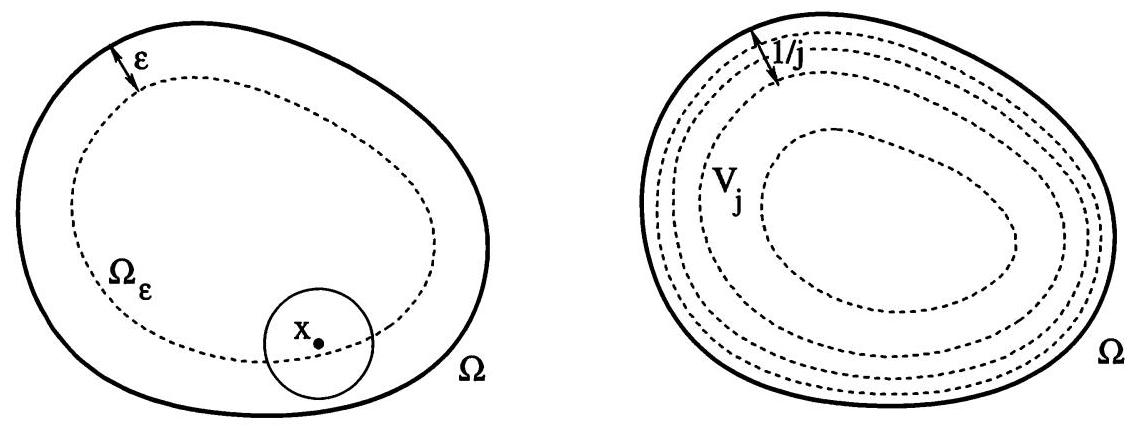
\includegraphics[width=0.85\textwidth]{images/bo_d6ik6nn7aajc739ct1l0_159_171_1175_1136_426_0.jpg}
\caption{左:到边界距离$> \varepsilon$ 的点构成的开子集 ${\Omega }_{\varepsilon } \subset  \Omega$ ；右:区域 $\Omega$ 可被可数个开子域 ${V}_{j} = {\Omega }_{1/\left( {j - 1}\right) } \setminus  {\overline{\Omega }}_{1/\left( {j + 1}\right) }$ 覆盖.}
\label{fig:omega-epsilon}
\end{figure}

引理\ref{lem:mollification}中所述磨光化的这一性质，为关联弱导数与经典意义下的偏导数提供了关键工具.作为首个应用，我们证明

\begin{corollary}[常值函数]\label{cor:constant-function}
设 $\Omega  \subseteq  {\mathbb{R}}^{n}$ 为连通开集，且假设 $u \in  {L}_{\text{ loc }}^{1}\left( \Omega \right)$ .若 $u$ 的一阶弱导数满足
\[
{D}_{{x}_{i}}u\left( x\right)  = 0,\;i = 1,2,\ldots ,n,\,\text{ a.e. }x \in  \Omega ,
\]

则 $u$ 几乎处处等于一常值函数.
\end{corollary}

\begin{proof}
1. 对 $\varepsilon  > 0$ ，考虑其磨光化函数 ${u}_{\varepsilon } = {J}_{\varepsilon } * u$ .由前述分析， ${u}_{\varepsilon } : {\Omega }_{\varepsilon } \mapsto  \mathbb{R}$ 是光滑函数，其导数 ${D}_{{x}_{i}}{u}_{\varepsilon }$ 在 ${\Omega }_{\varepsilon }$ 上恒为零.因此， ${u}_{\varepsilon }$ 在 ${\Omega }_{\varepsilon }$ 的每个连通分支上必为常数.

\noindent 2. 现考虑任意两点 $x,y \in  \Omega$ .由于开集 $\Omega$ 是连通的，故存在一条折线路径 $\Gamma$ ，连接 $x$ 与 $y$ ，且完全位于 $\Omega$ 内部.令 $\delta  \doteq  \mathop{\min }\limits_{{z \in  \Gamma }}d\left( {z,\partial \Omega }\right)  > 0$ 为 $\Gamma$ 中各点到 $\Omega$ 边界的最小距离.则对每个 $\varepsilon  < \delta$ ，整条折线 $\Gamma$ 均位于 ${\Omega }_{\varepsilon }$ 内.因此， $x,y$ 属于 ${\Omega }_{\varepsilon }$ 的同一连通分支.特别地， ${u}_{\varepsilon }\left( x\right)  = {u}_{\varepsilon }\left( y\right) .$ 

\noindent 3. 设 $\widetilde{u}\left( x\right)  \doteq  \mathop{\lim }\limits_{{\varepsilon  \rightarrow  0}}{u}_{\varepsilon }\left( x\right)$ .由前一步可知， $\widetilde{u}$ 在 $\Omega$ 上为常函数.此外， $\widetilde{u}\left( x\right)  = u\left( x\right)$ 在 $u$ 的每个Lebesgue点处成立，故在 $\Omega$ 上几乎处处成立.
\end{proof}

\begin{figure}[htbp]
\centering
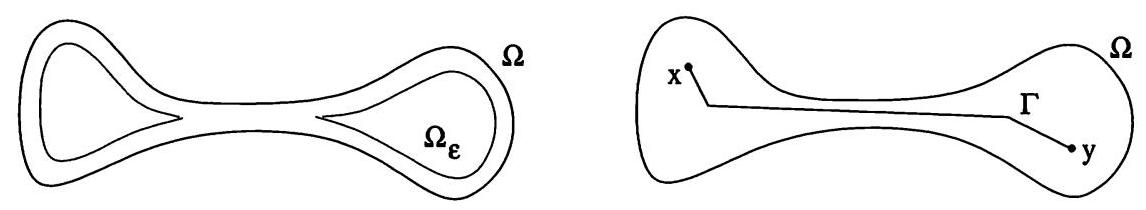
\includegraphics[width=0.9\textwidth]{images/bo_d6ik6nn7aajc739ct1l0_160_166_1087_1146_210_0.jpg}
\caption{左:即使 $\Omega$ 连通，子区域 ${\Omega }_{\varepsilon } \doteq \; \{ x \in  \Omega ;\bar{B}\left( {x,\varepsilon }\right)  \subseteq  \Omega \}$ 也可能不连通.右:任意两点 $x,y \in  \Omega$ 均可通过一条完全位于 $\Omega$ 内部的折线路径 $\Gamma$ 相连.因此，若 $\varepsilon  > 0$ 足够小，则 $x$ 与 $y$ 属于 ${\Omega }_{\varepsilon }$ 的同一连通分支.}
\label{fig:omega-epsilon-components}
\end{figure}

在一维情形下，再次借助引理\ref{lem:mollification}，我们现刻画具有 ${L}^{1}$ 中弱导数的函数集合.

\begin{corollary}[绝对连续函数]\label{cor:absolute-continuity}
设 $(a,b)$ 为一开区间，并设 $u \in  {L}_{\text{ loc }}^{1}\left(a,b\right)$ 具有弱导数 $v \in \; {L}^{1}\left( {( a,b) }\right)$ .则存在一个绝对连续函数 $\widetilde{u}$ ，使得
\begin{equation}\tag{8.14}\label{eq:ac-representative}
\widetilde{u}\left( x\right)  = u\left( x\right) \;\text{a.e. }x \in  ( a,b) ,
\end{equation}
\begin{equation}\tag{8.15}\label{eq:ac-classical-derivative}
v\left( x\right)  = \mathop{\lim }\limits_{{h \rightarrow  0}}\frac{\widetilde{u}\left( {x + h}\right)  - \widetilde{u}\left( x\right) }{h}\;\text{a.e. }x \in  ( a,b) .
\end{equation}
\end{corollary}

\begin{proof}
设 ${x}_{0} \in  ( a,b)$ 为 $u$ 的一个Lebesgue点，并定义
\[
\widetilde{u}\left( x\right)  \doteq  u\left( {x}_{0}\right)  + {\int }_{{x}_{0}}^{x}v\left( y\right) {\d y}.
\]

显然， $\widetilde{u}$ 绝对连续且满足\eqref{eq:ac-classical-derivative}.

为证\eqref{eq:ac-representative}，设 ${J}_{\varepsilon }$ 为标准磨光核，并令 ${u}_{\varepsilon } \doteq \; {J}_{\varepsilon } * u,{v}_{\varepsilon } \doteq  {J}_{\varepsilon } * v$ .则 ${u}_{\varepsilon },{v}_{\varepsilon } \in  {\mathcal{C}}^{\infty }\left( {( a + \varepsilon ,b - \varepsilon ) }\right)$ ，而引理\ref{lem:mollification}给出
\begin{equation}\tag{8.16}\label{eq:ac-mollified-fundamental}
{u}_{\varepsilon }\left( x\right)  = {u}_{\varepsilon }\left( {x}_{0}\right)  + {\int }_{{x}_{0}}^{x}{v}_{\varepsilon }\left( y\right) {\d y}\;\forall\,x \in  ( a + \varepsilon ,b - \varepsilon ) .
\end{equation}

令 $\varepsilon  \rightarrow  0$ ，我们得到 ${u}_{\varepsilon }\left( {x}_{0}\right)  \rightarrow  u\left( {x}_{0}\right)$ ，因为 ${x}_{0}$ 是一个Lebesgue点.此外，\eqref{eq:ac-mollified-fundamental}式右端对每个 $x \in  ( a,b)$ 均收敛于 $\widetilde{u}\left( x\right)$ ，而左端在 $u$ 的每个Lebesgue点(从而几乎处处)收敛于 $u\left( x\right)$ .因此\eqref{eq:ac-representative}成立.
\end{proof}
\begin{property}[弱可微函数]
若 $f,g \in  {L}_{\text{ loc }}^{1}\left( \Omega \right)$ 是弱可微函数，则对任意常数 $a,b \in  \mathbb{R}$ ，其线性组合 ${af} + {bg}$ 也弱可微，且满足
\begin{equation}\tag{8.17}\label{eq:weak-derivative-linearity}
{D}_{{x}_{i}}\left( {{af} + {bg}}\right)  = a{D}_{{x}_{i}}f + b{D}_{{x}_{i}}g.
\end{equation}
\end{property}



我们现在考虑弱可微函数的乘积与复合.需注意，一般地，两个函数 $f,g \in  {L}_{\text{ loc }}^{1}$ 的乘积未必是局部可求和的；类似地，定义在 ${\mathbb{R}}^{n}$ 上的两个弱可微函数的乘积也未必弱可微(参见习题 20).因此，在下一引理中，我们将假设其中一函数连续可微且其导数一致有界.

给定两个多重指标 $\alpha  = \left( {{\alpha }_{1},\ldots ,{\alpha }_{n}}\right)$ 和 $\beta  = \left( {{\beta }_{1},\ldots ,{\beta }_{n}}\right)$ ，我们回顾记号 $\beta  \leq  \alpha$ 表示对每个 $i = 1,\ldots ,n$ 均有 ${\beta }_{i} \leq  {\alpha }_{i}$ .此外，
\[
\begin{pmatrix}\alpha\\ \beta \end{pmatrix}\begin{pmatrix}\alpha\\ \beta \end{pmatrix}  \doteq  \frac{\alpha !}{\beta !\left( {\alpha  - \beta }\right) !} \doteq  \frac{{\alpha }_{1}!}{{\beta }_{1}!\left( {{\alpha }_{1} - {\beta }_{1}}\right) !} \cdot  \frac{{\alpha }_{2}!}{{\beta }_{2}!\left( {{\alpha }_{2} - {\beta }_{2}}\right) !}\cdots \frac{{\alpha }_{n}!}{{\beta }_{n}!\left( {{\alpha }_{n} - {\beta }_{n}}\right) !}.
\]
    
\begin{lemma}[弱可微函数的乘积与复合]\label{lem:weakly-differentiable-product-composition}
设 $\Omega  \subseteq  {\mathbb{R}}^{n}$ 为任意开集，并考虑函数 $u \in  {L}_{\text{ loc }}^{1}\left( \Omega \right)$ ，其具有任意阶 $\left| \alpha \right|  \leq  k$ 的弱导数 ${D}^{\alpha }u$ .
\begin{enumerate}[(i)]
    \item 若 $\eta  \in  {\mathcal{C}}^{k}\left( \Omega \right)$ ，则乘积 ${\eta u}$ 存在阶数不超过 $k$ 的弱导数.这些弱导数由莱布尼茨公式给出
\begin{equation}\tag{8.18}\label{eq:weak-leibniz}
{D}^{\alpha }\left( {\eta u}\right)  = \sum_{{\beta  \leq  \alpha }}\begin{pmatrix}\alpha\\ \beta \end{pmatrix} {D}^{\beta }\eta {D}^{\alpha  - \beta }u.
\end{equation}
    \item 设 ${\Omega }^{\prime } \subseteq  {\mathbb{R}}^{n}$ 为一开集， $\varphi  : {\Omega }^{\prime } \mapsto  \Omega$ 为一 ${\mathcal{C}}^{k}$ 双射，其雅可比矩阵具有一致有界逆.则复合函数 $u \circ  \varphi$ 属于 ${L}_{\text{ loc }}^{1}\left( {\Omega }^{\prime }\right)$ ，且存在阶数不超过 $k$ 的弱导数.
\end{enumerate}
\end{lemma}

\begin{proof}
1. 为证 (i)，令 ${J}_{\varepsilon }$ 为标准磨光子，并设 ${u}_{\varepsilon } \doteq  {J}_{\varepsilon } * u$ .由于莱布尼茨公式对光滑函数之乘积成立，故对每个 $\varepsilon  > 0$ ，我们得到
\begin{equation}\tag{8.19}\label{eq:weak-leibniz-mollified}
{D}^{\alpha }\left( {\eta {u}_{\varepsilon }}\right)  = \sum_{{\beta  \leq  \alpha }}\begin{pmatrix}\alpha\\ \beta \end{pmatrix} {D}^{\beta }\eta {D}^{\alpha  - \beta }{u}_{\varepsilon }.
\end{equation}

于是，对任一检验函数 $\phi  \in  {\mathcal{C}}_{c}^{\infty }\left( \Omega \right)$ ，有
{\begin{align*}
    {\left( -1\right) }^{\left| \alpha \right| }{\int }_{\Omega }\left( {\eta {u}_{\varepsilon }}\right) {D}^{\alpha }{\phi \d x} &= {\int }_{\Omega }{D}^{\alpha }\left( {\eta {u}_{\varepsilon }}\right) {\phi \d x} \\
    &= \sum_{{\beta  \leq  \alpha }}\begin{pmatrix}\alpha\\ \beta \end{pmatrix} {\int }_{\Omega }\left( {{D}^{\beta }\eta {D}^{\alpha  - \beta }{u}_{\varepsilon }}\right) {\phi \d x}.
\end{align*}}


注意:若 $\varepsilon  > 0$ 足够小，使得 $\operatorname{Supp}\left( \phi \right)  \subset  {\Omega }_{\varepsilon }$ ，则上述积分定义良好.令 $\varepsilon  \rightarrow  0$ ，可得
\[
{\left( -1\right) }^{\left| \alpha \right| }{\int }_{\Omega }\left( {\eta u}\right) {D}^{\alpha }{\phi \d x} = {\int }_{\Omega }\left( {\sum_{{\beta  \leq  \alpha }}\begin{pmatrix}\alpha\\ \beta \end{pmatrix} {D}^{\beta }\eta {D}^{\alpha  - \beta }u}\right) {\phi \d x}.
\]

由弱导数定义，式\eqref{eq:weak-leibniz}成立.

\noindent 2. 我们对 $k$ 归纳证明 (ii).记 $y$ 为 ${\Omega }^{\prime }$ 中的变量， $x = \varphi \left( y\right)$ 为 $\Omega$ 中的变量，如图\ref{fig:composition-map}所示.由假设， $n \times  n$ 雅可比矩阵 ${\left( \frac{\partial {\varphi }_{i}}{\partial {y}_{j}}\right) }_{i,j = 1,\ldots ,n}$ 具有一致有界逆.因此复合函数 $u \circ  \varphi$ 属于 ${L}_{\text{ loc }}^{1}\left( {\Omega }^{\prime }\right)$ ，从而定理在 $k = 0$ 情形下得证.

接下来，假设结论对所有阶数为 $\left| \alpha \right|  \leq \; k - 1$ 的弱导数均成立.取任一检验函数 $\phi  \in  {\mathcal{C}}_{c}^{\infty }\left( {\Omega }^{\prime }\right)$ ，并定义其磨光 ${u}_{\varepsilon } \doteq  {J}_{\varepsilon } * u$ .对任意足够小的 $\varepsilon  > 0$ 使得 $\varphi \left( {\operatorname{Supp}\left( \phi \right) }\right)  \subset  {\Omega }_{\varepsilon }$，有
{\begin{align*}
    - {\int }_{{\Omega }^{\prime }}\left( {{u}_{\varepsilon } \circ  \varphi }\right)  \cdot  {D}_{{y}_{i}}{\phi \d y} &= {\int }_{{\Omega }^{\prime }}{D}_{{y}_{i}}\left( {{u}_{\varepsilon } \circ  \varphi }\right)  \cdot  {\phi \d y}\\
    &= {\int }_{{\Omega }^{\prime }}\left( {\sum_{{j = 1}}^{n}{D}_{{x}_{j}}{u}_{\varepsilon }\left( {\varphi \left( y\right) }\right)  \cdot  {D}_{{y}_{i}}{\varphi }_{j}\left( y\right) }\right)  \cdot  \phi \left( y\right) {\d y}.
\end{align*}}

令 $\varepsilon  \rightarrow  0$ ，我们得出复合函数 $u \circ  \varphi$ 存在一阶弱导数，其表达式为
\begin{equation}\tag{8.20}\label{eq:weak-chain-rule}
{D}_{{y}_{i}}\left( {u \circ  \varphi }\right) \left( y\right)  = \sum_{{j = 1}}^{n}{D}_{{x}_{j}}u\left( {\varphi \left( y\right) }\right)  \cdot  {D}_{{y}_{i}}{\varphi }_{j}\left( y\right) .
\end{equation}

根据归纳假设，每个函数 ${D}_{{x}_{j}}\left( {u \circ  \varphi }\right)$ 均存在阶数不超过 $k - 1$ 的弱导数，而 ${D}_{{y}_{i}}{\varphi }_{j} \in  {\mathcal{C}}^{k - 1}\left( {\Omega }^{\prime }\right)$ .由引理第 (i) 部分可知，式\eqref{eq:weak-chain-rule}右端所有乘积均存在阶数不超过 $k - 1$ 的弱导数.再应用引理\ref{lem:weak-derivative-commute}，可得复合函数 $u \circ  \varphi$ 存在阶数不超过 $k$ 的弱导数.由此通过归纳法，证毕.
\end{proof}

\begin{figure}[htbp]
\centering
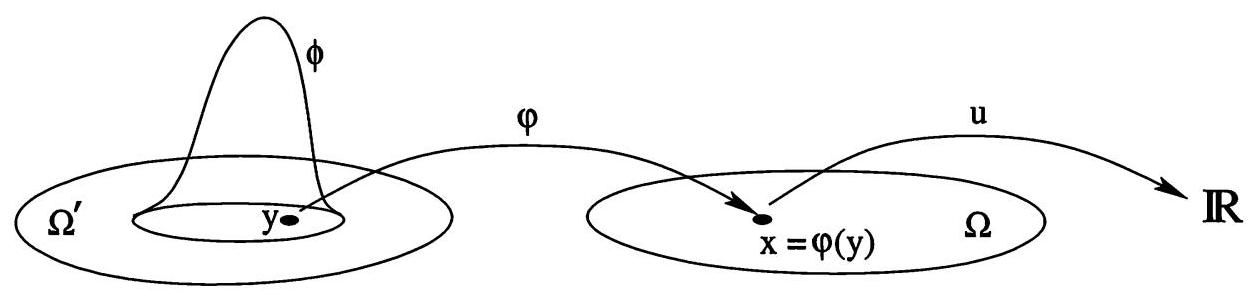
\includegraphics[width=1.0\textwidth]{images/bo_d6ik6nn7aajc739ct1l0_163_113_942_1254_295_0.jpg}
\caption{引理\ref{lem:weakly-differentiable-product-composition} 第 (ii) 部分所考虑的映射.}
\label{fig:composition-map}
\end{figure}

\section{Soblev空间}

考虑开集 $\Omega  \subseteq  {\mathbb{R}}^{n}$ ，固定 $p \in  \left(  {1,\infty }\right)$ ，并设 $k$ 为一非负整数.

\begin{definition}[Soblev空间]\label{def:sobolev-space}
(i) Soblev空间 ${W}^{k,p}\left( \Omega \right)$ 是指所有局部可积函数 $u : \Omega  \mapsto  \mathbb{R}$ 构成的空间，使得对每个满足 $\left| \alpha \right|  \leq  k$ 的多重指标 $\alpha$ ，其弱导数 ${D}^{\alpha }u$ 存在且属于 ${L}^{p}\left( \Omega \right)$ .

在 ${W}^{k,p}$ 上，我们采用如下范数:
\begin{equation}\tag{8.21}\label{eq:sobolev-norm-p}
\| u{\| }_{{W}^{k,p}} \doteq  {\left( \sum_{{\left| \alpha \right|  \leq  k}}{\int }_{\Omega }{\left| {D}^{\alpha }u\right| }^{p}\d x\right) }^{1/p},\;1 \leq  p < \infty ,
\end{equation}
\begin{equation}\tag{8.22}\label{eq:sobolev-norm-infty}
\| u{\| }_{{W}^{k,\infty }} \doteq  \sum_{{\left| \alpha \right|  \leq  k}}\underset{x \in  \Omega }{\operatorname{ess}\sup }\left| {{D}^{\alpha }u}\right|,\;p = \infty .
\end{equation}

(ii) 子空间 ${W}_{0}^{k,p}\left( \Omega \right)  \subseteq  {W}^{k,p}\left( \Omega \right)$ 定义为 ${\mathcal{C}}_{c}^{\infty }\left( \Omega \right)$ 在 ${W}^{k,p}\left( \Omega \right)$ 中的闭包.更准确地说， $u \in  {W}_{0}^{k,p}\left( \Omega \right)$ 当且仅当存在一列函数 ${u}_{n} \in  {\mathcal{C}}_{c}^{\infty }\left( \Omega \right)$ ，使得
\[
{\norm{u - u_n}}_{{W}^{k,p}} \rightarrow  0.
\]

(iii) 此外， ${W}_{\text{ loc }}^{k,p}\left( \Omega \right)$ 表示所有局部属于 ${W}^{k,p}$ 的函数构成的空间.这些函数 $u : \Omega  \mapsto  \mathbb{R}$ 满足如下性质:若开集 ${\Omega }^{\prime } \subset  \subset  \Omega$\footnotemark，则 $u$ 在 ${\Omega }^{\prime }$ 上的限制属于 ${W}^{k,p}\left( {\Omega }^{\prime }\right)$ .
\end{definition}
\footnotetext{根据定义，集合 ${\Omega }^{\prime }$ 紧包含于 $\Omega$ ，是指其闭包 $\overline{{\Omega }^{\prime }}$ 是 $\Omega$ 的一个紧子集.}

直观上，可将闭子空间 ${W}_{0}^{1,p}\left( \Omega \right)$ 视为所有在 $\Omega$ 边界上消失的函数 $u \in  {W}^{1,p}\left( \Omega \right)$ 构成的空间.更一般地， ${W}_{0}^{k,p}\left( \Omega \right)$ 是一类函数空间，其导数 ${D}^{\alpha }u$ 在 $\partial \Omega$ 上消失，其中 $\left| \alpha \right|  \leq  k - 1$ .

\begin{definition}[Hilbert-Soblev空间]\label{def:hilbert-sobolev-space}
在$p = 2$ 下，定义\colorbf{Hilbert-Soblev 空间}${H}^{k}\left( \Omega \right)  \doteq  {W}^{k,2}\left( \Omega \right)$，并赋予如下内积:
\begin{equation}\tag{8.23}\label{eq:hilbert-sobolev-inner-product}
\langle u,v{\rangle }_{{H}^{k}} \doteq  \sum_{{\left| \alpha \right|  \leq  k}}{\int }_{\Omega }{D}^{\alpha }u{D}^{\alpha }{v\d x}.
\end{equation}

类似地，定义 ${H}_{0}^{k}\left( \Omega \right)  \doteq  {W}_{0}^{k,2}\left( \Omega \right)$ .
\end{definition}

\begin{theorem}[Soblev空间的基本性质]\label{thm:sobolev-basic-properties}
(i) 每个 Soblev 空间 ${W}^{k,p}\left( \Omega \right)$ 都是一个 Banach 空间.

(ii) 空间 ${W}_{0}^{k,p}\left( \Omega \right)$ 是 ${W}^{k,p}\left( \Omega \right)$ 的一个闭子空间，因此它是一个 Banach 空间，且范数与 ${W}^{k,p}\left( \Omega \right)$ 相同.

(iii) 空间 ${H}^{k}\left( \Omega \right)$ 和 ${H}_{0}^{k}\left( \Omega \right)$ 均为 Hilbert 空间.
\end{theorem}

\begin{proof}
1. 设 $u,v \in  {W}^{k,p}\left( \Omega \right)$ .对 $\left| \alpha \right|  \leq  k$ ，称 ${D}^{\alpha }u,{D}^{\alpha }v$ 为其弱导数.则对任意 $\lambda ,\mu  \in  \mathbb{R}$，线性组合 ${\lambda u} + {\mu v}$ 是一个局部可和函数.易验证其弱导数为
\begin{equation}\tag{8.24}\label{eq:sobolev-weak-derivative-linearity}
{D}^{\alpha }\left( {{\lambda u} + {\mu v}}\right)  = \lambda {D}^{\alpha }u + \mu {D}^{\alpha }v.
\end{equation}
因此，对每个 $\left| \alpha \right|  \leq  k$ ，有 ${D}^{\alpha }\left( {{\lambda u} + {\mu v}}\right)  \in  {L}^{p}\left( \Omega \right)$ .这表明 ${W}^{k,p}\left( \Omega \right)$ 是一个向量空间.


\noindent 2. 接下来验证式\eqref{eq:sobolev-norm-p}与式\eqref{eq:sobolev-norm-infty}满足定义范数的条件 (N1)-(N3).对 $\lambda  \in  \mathbb{R}$ 和 $u \in  {W}^{k,p}$ ，有
\begin{gather*}
    \| {\lambda u}{\| }_{{W}^{k,p}} = \left| \lambda \right| \| u{\| }_{{W}^{k,p}}\\
    \| u{\| }_{{W}^{k,p}} \geq  \| u{\| }_{{L}^{p}} \geq  0
\end{gather*}
且等号成立当且仅当 $u = 0$ .

此外，若 $u,v \in  {W}^{k,p}\left( \Omega \right)$ ，则对 $1 \leq  p < \infty$ ，Minkowski不等式给出
{\begin{align*}
    \| u + v{\| }_{{W}^{k,p}} &= {\left( \sum_{{\left| \alpha \right|  \leq  k}}{\norm{{D}^{\alpha }u + {D}^{\alpha }v}_{{L}^{p}}^{p}}\right) }^{1/p}\\
    &\leq  {\left( \sum_{{\left| \alpha \right|  \leq  k}}{\left( {\norm{D^{\alpha }u}}_{{L}^{p}} + {\norm{D^{\alpha }v}}_{{L}^{p}}\right) }^{p}\right) }^{1/p}\\
    &\leq  {\left( \sum_{{\left| \alpha \right|  \leq  k}}{\norm{D^{\alpha }u}_{{L}^{p}}^{p}}\right) }^{1/p} + {\left( \sum_{{\left| \alpha \right|  \leq  k}}{\norm{D^{\alpha }v}_{{L}^{p}}^{p}}\right) }^{1/p}\\
    &= \| u{\| }_{{W}^{k,p}} + \| v{\| }_{{W}^{k,p}}.
\end{align*}}

在 $p = \infty$ 的情形下，上述计算替换为
{\begin{align*}
    \| u + v{\| }_{{W}^{k,\infty }} &= \sum_{{\left| \alpha \right|  \leq  k}}{\norm{D^{\alpha }u + {D}^{\alpha }v}}_{{L}^{\infty }} \leq  \sum_{{\left| \alpha \right|  \leq  k}}\left( {{\norm{D^{\alpha }u}}_{{L}^{\infty }} + {\norm{D^{\alpha }v}}_{{L}^{\infty }}}\right)\\
    &= \| u{\| }_{{W}^{k,\infty }} + \| v{\| }_{{W}^{k,\infty }}.
\end{align*}}


\noindent 3. 为完成 (i) 的证明，需证空间 ${W}^{k,p}\left( \Omega \right)$ 是完备的，故为 Banach 空间.

设 ${\left( {u}_{n}\right) }_{n \geq  1}$ 是 ${W}^{k,p}\left( \Omega \right)$ 中的一个 Cauchy 序列.对任一满足 $\left| \alpha \right|  \leq  k$ 的多重指标 $\alpha$ ，弱导数序列 ${D}^{\alpha }{u}_{n}$ 在 ${L}^{p}\left( \Omega \right)$ 中为 Cauchy 序列.由于 ${L}^{p}\left( \Omega \right)$ 完备，故存在函数 $u$ 和 ${u}_{\alpha }$ ，使得
\begin{equation}\tag{8.25}\label{eq:sobolev-cauchy-convergence}
\| {u}_{n} - u{\| }_{{L}^{p}} \rightarrow  0,\;\| {D}^{\alpha }{u}_{n} - {u}_{\alpha }{\| }_{{L}^{p}} \rightarrow  0\;\forall\,\left| \alpha \right|  \leq  k.
\end{equation}

由引理\ref{lem:weak-derivative-convergence}，极限函数 ${u}_{\alpha }$ 恰为弱导数 ${D}^{\alpha }u$ .因该结论对所有满足 $\left| \alpha \right|  \leq  k$ 的多重指标 $\alpha$ 成立，故收敛 ${u}_{n} \rightarrow \; u$ 在 ${W}^{k,p}\left( \Omega \right)$ 中成立.至此，(i) 得证.

\noindent 4. ${W}_{0}^{k,p}\left( \Omega \right)$ 是 ${W}^{k,p}\left( \Omega \right)$ 的闭子空间这一事实直接由定义得出.同样易验证式\eqref{eq:hilbert-sobolev-inner-product}是一个内积，其所诱导的范数为 $\|  \cdot  {\| }_{{W}^{k,2}}$ .
\end{proof}

\begin{instance}\label{ins:W1p-interval-ac}
设 $\Omega = (a,b)$ 为一开区间.由推论\ref{cor:absolute-continuity}可知，空间 ${W}^{1,p}\left( {( a,b) }\right)$ 的每个元素几乎处处等于某个绝对连续函数 $f : (a,b) \mapsto  \mathbb{R}$ ，且该函数的导数为 ${f}^{\prime } \in  {L}^{p}\left( {( a,b) }\right)$ .\par
\begin{figure}[htbp]
\centering
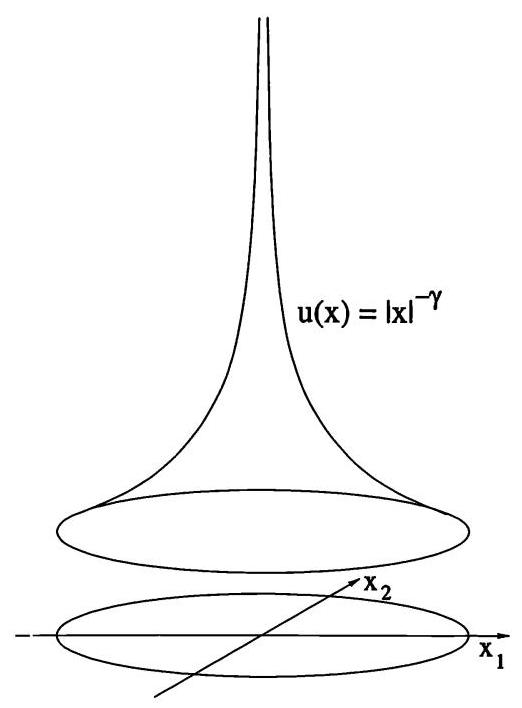
\includegraphics[width=0.35\textwidth]{images/bo_d6ik6nn7aajc739ct1l0_166_479_682_522_708_0.jpg}
\caption{对某些 $p,n$ 取值，函数 $u \in  {W}^{1,p}\left( {\mathbb{R}}^{n}\right)$ 可能不连续或无界.}
\label{fig:W1p-discontinuous}
\end{figure}
\end{instance}



\begin{instance}\label{ins:radial-singularity-W1p}
设 $\Omega  = B\left( {0,1}\right)  \subset  {\mathbb{R}}^{n}$ 为以原点为中心、半径为一的开球.固定 $\gamma  > 0$ ，并考虑径向对称函数
\[
u\left( x\right)  \doteq  {\left| x\right| }^{-\gamma } = {\left( \sum_{{i = 1}}^{n}{x}_{i}^{2}\right) }^{-\gamma /2},\;0 < \left| x\right|  < 1.
\]

注意到 $u \in  {\mathcal{C}}^{1}\left( {\Omega \setminus \{ 0\} }\right)$ .我们声称:对 $1 \leq  p < \infty$ ，
\begin{equation}\tag{8.26}\label{eq:radial-W1p-condition}
u \in  {W}^{1,p}\left( \Omega \right)\iff \gamma  < \frac{n - p}{p}.
\end{equation}

在原点之外，偏导数计算如下:
\begin{equation}\tag{8.27}\label{eq:radial-W1p-derivative}
{u}_{{x}_{i}} =  - \frac{\gamma }{2}{\left( \sum_{{i = 1}}^{n}{x}_{i}^{2}\right) }^{-\left( {\gamma /2}\right)  - 1}2{x}_{i} = \frac{-\gamma {x}_{i}}{{\left| x\right| }^{\gamma  + 2}}.
\end{equation}

因此，梯度 $\nabla u = \left( {{u}_{{x}_{1}},\ldots ,{u}_{{x}_{n}}}\right)$ 的欧氏范数为
\[
\left| {\nabla u\left( x\right) }\right|  = {\left( \sum_{{i = 1}}^{n}{\left| {u}_{{x}_{i}}\left( x\right) \right| }^{2}\right) }^{1/2} = \frac{\gamma }{{\left| x\right| }^{\gamma  + 1}}.
\]

记 ${\sigma }_{n}$ 为单位球面 $\{ x \in  {\mathbb{R}}^{n};\left| x\right|  = 1\}$ 的 $\left( {n - 1}\right)$ 维测度，我们计算得
\begin{equation}\tag{8.28}\label{eq:radial-W1p-integral}
    \setjot[-2]\begin{aligned}
        {\int }_{\Omega }{\left( \frac{1}{{\left| x\right| }^{\gamma  + 1}}\right) }^{p}{\d x} &= {\int }_{x \in  {\mathbb{R}}^{n},\left| x\right|  < 1}{\left| x\right| }^{-p\left( {\gamma  + 1}\right) }{\d x}\\
        &= {\sigma }_{n}{\int }_{0}^{1}{r}^{n - 1}{r}^{-p\left( {\gamma  + 1}\right) }{\d r}.
    \end{aligned}
\end{equation}

式\eqref{eq:radial-W1p-integral}右端有限当且仅当 $n - 1 - p\left( {\gamma  + 1}\right)  >  - 1$ ，即 $\gamma  < \frac{n - p}{p}$ .对 ${\left| u\right| }^{p}$ 作类似计算后，我们得出
\[
{\int }_{\Omega }\left( {{\left| u\right| }^{p} + {\left| \nabla u\right| }^{p}}\right) {\d x} < \infty \iff \gamma  < \frac{n - p}{p}.
\]

为完成式\eqref{eq:radial-W1p-condition}的证明，需验证:若 $0 < \gamma  < \frac{n - p}{p}$ (从而 $n \geq  2$ )，则式\eqref{eq:radial-W1p-derivative}中所定义的函数确为 $u$ 在整个球 $\Omega$ 上的弱导数(而不仅限于集合 $\Omega  \setminus  \{ 0\}$ 上).为此，取任意检验函数 $\phi  \in  {\mathcal{C}}_{c}^{\infty }\left( \Omega \right)$ .固定 $i \in  \{ 1,\ldots ,n\}$ .为方便起见，我们将 $\phi$ 延拓至整个空间 ${\mathbb{R}}^{n}$ ，即令 $\phi \left( x\right)  = 0$ 对所有 $x \notin  \Omega$ 成立.由于 $n \geq  2$ ， ${x}_{i}$ 轴的 $n$ 维 Lebesgue 测度为零.分部积分得
{\setjot[-2]\begin{align*}
    {\int }_{\Omega }\frac{-\gamma {x}_{i}}{{\left| x\right| }^{\gamma  + 2}}{\phi \d x} &= {\int }_{{\mathbb{R}}^{n - 1}\setminus \{ 0\} }\left( {{\int }_{\mathbb{R}}\frac{-\gamma {x}_{i}}{{\left| x\right| }^{\gamma  + 2}}\phi {\d x_{i}}}\right) \d x_{1}\cdots \d x_{i - 1}\d x_{i + 1}\cdots \d x_{n}\\
    &=  - {\int }_{{\mathbb{R}}^{n - 1}\setminus \{ 0\} }\left( {{\int }_{\mathbb{R}}{\left| x\right| }^{-\gamma }{\phi }_{{x}_{i}}\d x_{i}}\right) \d x_{1}\cdots \d x_{i - 1}\d x_{i + 1}\cdots \d x_{n}\\
    &=  - {\int }_{\Omega }{\left| x\right| }^{-\gamma }{\phi }_{{x}_{i}}{\d x}.
\end{align*}}


注意，前述计算依赖于 $u$ 在几乎每条平行于某坐标轴的直线上绝对连续(事实上光滑)这一事实.然而，无法通过在零测集上修改 $u$ ，使其在整个区域 $\Omega$ 上连续.
\end{instance}

Soblev空间中其一重要问题是:能否用函数一阶导数的范数来估计该函数的范数？ \par
以下结果为此提供了初等估计.它对包含于某一层状区域(例如) $\Omega$ 的区域成立.
\begin{equation}\tag{8.29}\label{eq:poincare-strip-domain}
\Omega  \subseteq  \left\{  {x = \left( {{x}_{1},{x}_{2},\ldots ,{x}_{n}}\right) ;a < {x}_{1} < b}\right\}  .
\end{equation}

\begin{theorem}[Poincaré不等式，I]\label{thm:poincare-inequality-I}
设 $\Omega  \subset  {\mathbb{R}}^{n}$ 是满足式\eqref{eq:poincare-strip-domain}的某个 $a,b \in  \mathbb{R}$ 的开集.则每个 $u \in  {H}_{0}^{1}\left( \Omega \right)$ 均满足
\begin{equation}\tag{8.30}\label{eq:poincare-inequality-I}
\| u{\| }_{{L}^{2}\left( \Omega \right) }\; \leq  \;2\left( {b - a}\right) \;\| {D}_{{x}_{1}}u{\| }_{{L}^{2}\left( \Omega \right) }.
\end{equation}
\end{theorem}

\begin{proof}
1. 首先假设 $u \in  {\mathcal{C}}_{c}^{\infty }\left( \Omega \right)$ .我们将 $u$ 延拓至全空间 ${\mathbb{R}}^{n}$ ，定义为对 $x \notin  \Omega$ 取 $u\left( x\right)  = 0$ .引入变量 $x = \left( {{x}_{1},{x}^{\prime }}\right)$ ，其中 ${x}^{\prime } = \left( {{x}_{2},\ldots ,{x}_{n}}\right)$ ，计算得
\[
{u}^{2}\left( {{x}_{1},{x}^{\prime }}\right)  = {\int }_{a}^{{x}_{1}}{2u}{u}_{{x}_{1}}\left( {t,{x}^{\prime }}\right) {\d t}.
\]

分部积分得
{\setjot[-2]\begin{align*}
    \| u{\| }_{{L}^{2}}^{2} &= {\int }_{{\mathbb{R}}^{n}}{u}^{2}\left( x\right) {\d x} = {\int }_{{\mathbb{R}}^{n - 1}}{\int }_{a}^{b}1 \cdot  \left( {{\int }_{a}^{{x}_{1}}{2u}{u}_{{x}_{1}}\left( {t,{x}^{\prime }}\right) {\d t}}\right) \d x_{1}\d x^{\prime }\\
    &= {\int }_{{\mathbb{R}}^{n - 1}}{\int }_{a}^{b}\left( {b - {x}_{1}}\right) {2u}{u}_{{x}_{1}}\left( {{x}_{1},{x}^{\prime }}\right) \d x_{1}\d x^{\prime } \leq  2\left( {b - a}\right) {\int }_{{\mathbb{R}}^{n}}\left| u\right| \left| {u}_{{x}_{1}}\right| {\d x}\\
    &\leq  2\left( {b - a}\right) \| u{\| }_{{L}^{2}}{\norm{u}_{{x}_{1}}}_{{L}^{2}}
\end{align*}}


两边同除以 $\| u{\| }_{{L}^{2}}$ ，即得对每个 $u \in  {\mathcal{C}}_{c}^{\infty }\left( \Omega \right)$ 成立的式\eqref{eq:poincare-inequality-I}.

\noindent 2. 现考虑任意 $u \in  {H}_{0}^{1}\left( \Omega \right)$ .由假设，存在函数列 ${u}_{n} \in  {\mathcal{C}}_{c}^{\infty }\left( \Omega \right)$，使得 ${\norm{u}_{n} - u}_{{H}^{1}} \rightarrow  0$.由前一步可知
\[
\| u{\| }_{{L}^{2}} = \mathop{\lim }\limits_{{n \rightarrow  \infty }}{\norm{u}_{n}}_{{L}^{2}} \leq  \mathop{\lim }\limits_{{n \rightarrow  \infty }}2\left( {b - a}\right) {\norm{D_{{x}_{1}}{u}_{n}}}_{{L}^{2}} = 2\left( {b - a}\right) {\norm{D_{{x}_{1}}u}}_{{L}^{2}}.\qedhere
\]
\end{proof}

为继续分析Soblev空间，我们需要建立关于弱导数的一些额外事实.

\begin{theorem}[弱导数的性质]\label{thm:weak-derivative-properties}
设 $\Omega  \subseteq  {\mathbb{R}}^{n}$ 为开集， $p \in  \left(  {1,\infty }\right)$ ，且 $\left| \alpha \right|  \leq  k$ .若 $u,v \in  {W}^{k,p}\left( \Omega \right)$ ，则:
\begin{enumerate}
    \item $u$ 在任意开集 $\widetilde{\Omega } \subset  \Omega$ 上的限制属于空间 ${W}^{k,p}\left( \widetilde{\Omega }\right)$ .
    \item ${D}^{\alpha }u \in  {W}^{k - \left| \alpha \right| ,p}\left( \Omega \right)$ .
    \item 若 $\eta  \in  {\mathcal{C}}^{k}\left( \Omega \right)$ ，则乘积满足 ${\eta u} \in  {W}^{k,p}\left( \Omega \right)$ .此外，存在仅依赖于 $\Omega$ 和 $\| \eta {\| }_{{\mathcal{C}}^{k}}$，但不依赖于 $u,$ 的常数 $C$ ，使得
\begin{equation}\tag{8.31}\label{eq:eta-u-Wkp-estimate}
\norm{\eta u}_{{W}^{k,p}\left( \Omega \right) } \leq C\norm{u}_{{W}^{k,p}\left( \Omega \right) }.
\end{equation}
    \item 设 ${\Omega }^{\prime } \subseteq  {\mathbb{R}}^{n}$ 为开集， $\varphi  : {\Omega }^{\prime } \mapsto  \Omega$ 为 ${\mathcal{C}}^{k}$ 微分同胚，其Jacobi矩阵的逆一致有界.则复合函数满足 $u \circ  \varphi  \in  {W}^{k,p}\left( {\Omega }^{\prime }\right)$ .此外，存在仅依赖于 ${\Omega }^{\prime }$ 和 $\| \varphi {\| }_{{\mathcal{C}}^{k}}$ 、但不依赖于 $u$ 的常数 $C$ ，使得
\begin{equation}\tag{8.32}\label{eq:composition-Wkp-estimate}
\norm{u \circ  \varphi }_{{W}^{k,p}\left( {\Omega }^{\prime }\right) }\leq  C\norm{u}_{{W}^{k,p}\left( \Omega \right) }.
\end{equation}
\end{enumerate}
\end{theorem}

\begin{proof}
命题 (i) 是定义的直接推论，而 (ii) 由引理\ref{lem:weak-derivative-commute}得出.

为证 (iii)，我们注意到:由假设， $\eta$ 的所有导数均有界，即
\[
{\norm{D^{\beta }\eta }}_{{L}^{\infty }} \leq  \| \eta {\| }_{{\mathcal{C}}^{k}},\;\forall\,\left| \beta \right|  \leq  k.
\]

因此，由表示公式\eqref{eq:weak-leibniz}即得估计式\eqref{eq:eta-u-Wkp-estimate}.

回顾引理\ref{lem:weakly-differentiable-product-composition}的第(ii)部分，我们对 $k$ 作归纳法证明 (iv).由假设， $n \times  n$ 雅可比矩阵 ${\left( {D}_{{x}_{i}}{\varphi }_{j}\right) }_{i,j = 1,\ldots ,n}$ 具有一致有界逆.因此 $k = 0$ 的情形显然成立.

接下来，假设结论对 $k = 0,1,\ldots ,m - 1$ 成立.若 $u \in \; {W}^{m,p}\left( \Omega \right)$ ，则有
\[
\| {D}_{{x}_{i}}\left( {u \circ  \varphi }\right) {\| }_{{W}^{m - 1,p}\left( {\Omega }^{\prime }\right) }\; \leq  \;{C}^{\prime }\;\| \nabla u{\| }_{{W}^{m - 1,p}\left( \Omega \right) }\| \varphi {\| }_{{\mathcal{C}}^{m}\left( {\Omega }^{\prime }\right) }\; \leq  \;C\;\| u{\| }_{{W}^{m,p}\left( \Omega \right) }.
\]

表明结论对 $k = m$ 亦成立.由归纳法，结论成立.
\end{proof}

\section{Soblev函数的逼近}

若 $u \in  {W}^{k,p}\left( {\mathbb{R}}^{n}\right)$ 是定义在整个空间 ${\mathbb{R}}^{n}$ 上的函数，则可通过取磨光来简单地用光滑函数逼近: ${u}_{\varepsilon } = \; {J}_{\varepsilon } * u$ .然而，若 $u$ 仅定义在某个开子集 $\Omega  \subset  {\mathbb{R}}^{n}$ 上，则需更精细的构造.

\begin{theorem}[用光滑函数逼近]\label{thm:approximation-by-smooth-functions}
设 $\Omega  \subseteq  {\mathbb{R}}^{n}$ 为开集， $u \in  {W}^{k,p}\left( \Omega \right)$ 满足 $1 \leq  p < \infty$ .则对任意 $\varepsilon  > 0$ ，存在函数 $U \in  {\mathcal{C}}^{\infty }\left( \Omega \right)$ 使得 $\| U - u{\| }_{{W}^{k,p}\left( \Omega \right) } < \varepsilon$ .
\end{theorem}

\begin{proof}
1. 给定 $\varepsilon  > 0$ .考虑集合 $\Omega$ 的如下局部有限开覆盖(见图\ref{fig:omega-epsilon}):
\begin{gather*}
{V}_{1} \doteq  \left\{  {x \in  \Omega ;d\left( {x,\partial \Omega }\right)  > \frac{1}{2}}\right\}\\
{V}_{j} \doteq  \left\{  {x \in  \Omega ;\frac{1}{j + 1} < d\left( {x,\partial \Omega }\right)  < \frac{1}{j - 1}}\right\}  ,\;j = 2,3,\ldots
\end{gather*}

利用附录中定理A.18，令 ${\eta }_{1},{\eta }_{2},\ldots$ 为从属于上述覆盖的光滑单位分解.由定理\ref{thm:weak-derivative-properties}，对每个 $j \geq  0$ ，乘积 ${\eta }_{j}u$ 属于 ${W}^{k,p}\left( \Omega \right)$ .依构造，其支集包含于 ${V}_{j}$ .

\noindent 2. 考虑磨光 ${J}_{\varepsilon } * \left( {{\eta }_{j}u}\right)$ .由引理\ref{lem:mollification}及附录中定理A.16，对每个 $\left| \alpha \right|  \leq  k$ ，有
\[
{D}^{\alpha }\left( {{J}_{\varepsilon } * \left( {{\eta }_{j}u}\right) }\right)  = {J}_{\epsilon } * \left( {{D}^{\alpha }\left( {{\eta }_{j}u}\right) }\right)  \rightarrow  {D}^{\alpha }\left( {{\eta }_{j}u}\right),\varepsilon\to 0
\]

由于每个 ${\eta }_{j}$ 具有紧支集，此处收敛在 ${L}^{p}\left( \Omega \right)$ 中发生.因此，对每个 $j \geq  0$ ，可取 $0 < {\varepsilon }_{j} < {2}^{-j}$ 足够小使得
\[
{\norm{\eta _{j}u - {J}_{{\varepsilon }_{j}} * \left( {\eta }_{j}u\right) }}_{{W}^{k,p}\left( \Omega \right) } \leq  \varepsilon {2}^{-j}.
\]

\noindent 3. 考虑函数
\[
U \doteq  \sum_{{j = 1}}^{\infty }{J}_{{\varepsilon }_{j}} * \left( {{\eta }_{j}u}\right)
\]

注意，上述级数在 ${W}^{k,p}$ 中未必收敛.但其必逐点收敛，因为任一紧集 $K \subset  \Omega$ 仅与有限个集合 ${V}_{j}$ 相交.限制在 $K$ 上时，上述和式仅含有限个非零项.由于每项均光滑，故有 $U \in \; {\mathcal{C}}^{\infty }\left( \Omega \right)$ .

\noindent 4. 考虑子区域
\[
{\Omega }_{1/n} \doteq  \left\{  {x \in  \Omega ;d\left( {x,\partial \Omega }\right)  > \frac{1}{n}}\right\}  .
\]

由 $\sum_{j}{\eta }_{j}\left( x\right)  \equiv  1$ 可知，对每个 $n \geq  1$ ，得到
\[
\| U - u{\| }_{{W}^{k,p}\left( {\Omega }_{1/n}\right) } \leq  \sum_{{j = 1}}^{{n + 2}}{\norm{\eta _{j}u - {J}_{{\varepsilon }_{j}} * \left( {\eta }_{j}u\right) }}_{{W}^{k,p}\left( {\Omega }_{1/n}\right) } \leq  \sum_{{j = 1}}^{{n + 2}}\varepsilon {2}^{-j} \leq  \varepsilon .
\]

由此推出
\[
\norm{U - u}_{{W}^{k,p}\left( \Omega \right) } = \mathop{\sup }\limits_{{n \geq  1}}\norm{U - u}_{{W}^{k,p}\left( {\Omega }_{1/n}\right) } \leq  \varepsilon .
\]

由于 $\varepsilon  > 0$ 是任意的，这证明了 ${\mathcal{C}}^{\infty }$ 函数集在 ${W}^{k,p}\left( \Omega \right)$ 中稠密.
\end{proof}

利用上述逼近结果，我们得到Soblev函数的第一个正则性定理(见图\ref{fig:omega-cylinder-domain}).

\begin{theorem}[弱导数与强导数之间的关系]\label{thm:weak-strong-derivative}
设 $u \in  {W}^{1,1}\left( \Omega \right)$ ，其中 $\Omega  \subseteq  {\mathbb{R}}^{n}$ 为具有如下形式的开集\eqref{eq:omega-cylinder-domain}
\begin{equation}\tag{8.33}\label{eq:omega-cylinder-domain}
\Omega  = \left\{  {x = \left( {x,{x}^{\prime }}\right) ;{x}^{\prime } \doteq  \left( {{x}_{2},\ldots ,{x}_{n}}\right)  \in  {\Omega }^{\prime },\alpha \left( {x}^{\prime }\right)  < {x}_{1} < \beta \left( {x}^{\prime }\right) }\right\}
\end{equation}

(可能取 $\alpha  \equiv   - \infty$ 或 $\beta  \equiv   + \infty$ ).则存在函数 $\widetilde{u}$ ，使得对几乎处处的 $x \in  \Omega$ ，有 $\widetilde{u}\left( x\right)  = u\left( x\right)$ ，且满足以下条件:对几乎处处的 ${x}^{\prime } = \; \left( {{x}_{2},\ldots ,{x}_{n}}\right)  \in  {\Omega }^{\prime } \subset  {\mathbb{R}}^{n - 1}$ (关于 $\left( {n - 1}\right)$ 维Lebesgue测度)，映射
\[
{x}_{1} \mapsto  \widetilde{u}\left( {{x}_{1},{x}^{\prime }}\right)
\]

是绝对连续的；其导数几乎处处等于弱导数 ${D}_{{x}_{1}}u$ .
\end{theorem}

\begin{figure}[htbp]
\centering
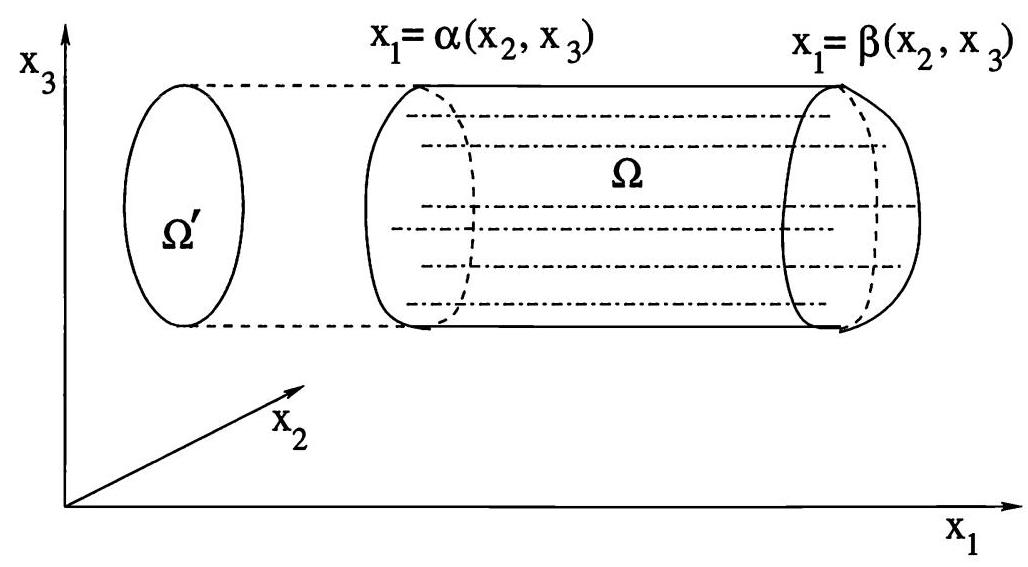
\includegraphics[width=0.9\textwidth]{images/bo_d6ik6nn7aajc739ct1l0_171_221_1182_1028_567_0.jpg}
\caption{\eqref{eq:omega-cylinder-domain}式中的定义域 $\Omega$ .若 $u$ 具有弱导数 ${D}_{{x}_{1}}u \in  {L}^{1}\left( \Omega \right)$ ，则(通过在零测集上修改其取值)函数 $u$ 在几乎每条平行于 ${x}_{1}$ 轴的线段上绝对连续，且其偏导数 $\partial u/\partial {x}_{1}$ 几乎处处等于该弱导数.}
\label{fig:omega-cylinder-domain}
\end{figure}

\begin{proof}
1. 由定理\ref{thm:approximation-by-smooth-functions}，存在一列函数 ${u}_{k} \in  {\mathcal{C}}^{\infty }\left( \Omega \right)$ ，使得
\begin{equation}\tag{8.34}\label{eq:uk-converge-W11}
{\norm{u}_{k} - u}_{{W}^{1,1}} < {2}^{-k}
\end{equation}

我们断言，这蕴含逐点收敛性
\[
{u}_{k}\left( x\right)  \rightarrow  u\left( x\right) ,\;{D}_{{x}_{1}}{u}_{k}\left( x\right)  \rightarrow  {D}_{{x}_{1}}u\left( x\right) \;\text{ for a.e. }x \in  \Omega .
\]

事实上，考虑函数
\begin{equation}\tag{8.35}\label{eq:def-fg-series}
{\setjot[-2]\begin{aligned}
f\left( x\right)  &\doteq  \left| {{u}_{1}\left( x\right) }\right|  + \sum_{{k = 1}}^{\infty }\left| {{u}_{k + 1}\left( x\right)  - {u}_{k}\left( x\right) }\right| \\
g\left( x\right)  &\doteq  \left| {{D}_{{x}_{1}}{u}_{1}\left( x\right) }\right|  + \sum_{{k = 1}}^{\infty }\left| {{D}_{{x}_{1}}{u}_{k + 1}\left( x\right)  - {D}_{{x}_{1}}{u}_{k}\left( x\right) }\right| .
\end{aligned}}
\end{equation}

由\eqref{eq:uk-converge-W11}，
\[
{\norm{u}_{k} - {u}_{k + 1}}_{{W}^{1,1}} \leq  {2}^{1 - k}
\]

因此 $f,g \in  {L}^{1}\left( \Omega \right)$ ，且\eqref{eq:def-fg-series}式中的级数对几乎处处的 $x \in  \Omega$ 绝对收敛，故其几乎处处逐点收敛.此外，我们还有如下估计
\begin{equation}\tag{8.36}\label{eq:uk-bounded-by-fg}
\left| {{u}_{k}\left( x\right) }\right| \leq  f\left( x\right) ,\quad \left| {{D}_{{x}_{1}}{u}_{k}\left( x\right) }\right| \leq  g\left( x\right),\forall\,k \geq  1,\;x \in  \Omega .
\end{equation}

\noindent 2. 由于 $f,g \in  {L}^{1}\left( \Omega \right)$ ，由Fubini定理，存在一个零测集 $\mathcal{N} \subset  {\Omega }^{\prime }$ (关于 $\left( {n - 1}\right)$ 维Lebesgue测度)，使得对每个 ${x}^{\prime } \in  {\Omega }^{\prime } \setminus  \mathcal{N}$ ，均有
\begin{equation}\tag{8.37}\label{eq:fg-integrable-slices}
{\int }_{\alpha \left( {x}^{\prime }\right) }^{\beta \left( {x}^{\prime }\right) }f\left( {{x}_{1},{x}^{\prime }}\right) \d x_{1} < \infty ,\quad {\int }_{\alpha \left( {x}^{\prime }\right) }^{\beta \left( {x}^{\prime }\right) }g\left( {{x}_{1},{x}^{\prime }}\right) \d x_{1} < \infty .
\end{equation}

固定这样一个点 ${x}^{\prime } \in  {\Omega }^{\prime } \setminus  \mathcal{N}$ .选取一点 ${y}_{1} \in  ( \alpha \left( {x}^{\prime }\right) ,\beta \left( {x}^{\prime }\right) )$ ，使得逐点收敛 ${u}_{k}\left( {{y}_{1},{x}^{\prime }}\right)  \rightarrow  u\left( {{y}_{1},{x}^{\prime }}\right)$ 成立.对任意 $\alpha \left( {x}^{\prime }\right)  < {x}_{1} < \; \beta \left( {x}^{\prime }\right)$ ，因 ${u}_{k}$ 光滑，故有
\begin{equation}\tag{8.38}\label{eq:uk-line-integral}
{u}_{k}\left( {{x}_{1},{x}^{\prime }}\right)  = {u}_{k}\left( {{y}_{1},{x}^{\prime }}\right)  + {\int }_{{y}_{1}}^{{x}_{1}}{D}_{{x}_{1}}{u}_{k}\left( {s,{x}^{\prime }}\right) {\d s}.
\end{equation}

现令 $k \rightarrow  \infty$ 趋于\eqref{eq:uk-line-integral}式中右侧极限.由\eqref{eq:uk-bounded-by-fg}与\eqref{eq:fg-integrable-slices}，函数 ${D}_{{x}_{1}}{u}_{k}\left( {\cdot ,{x}^{\prime }}\right)$ 均被可积函数 $g\left( {\cdot ,{x}^{\prime }}\right)  \in  {L}^{1}$ 控制.根据控制收敛定理，\eqref{eq:uk-line-integral}式右侧从而收敛于
\begin{equation}\tag{8.39}\label{eq:def-u-tilde}
\widetilde{u}\left( {{x}_{1},{x}^{\prime }}\right)  \doteq  u\left( {{y}_{1},{x}^{\prime }}\right)  + {\int }_{{y}_{1}}^{{x}_{1}}{D}_{{x}_{1}}u\left( {s,{x}^{\prime }}\right) {\d s}.
\end{equation}

显然，\eqref{eq:def-u-tilde}式右侧是标量变量 ${x}_{1}$ 的绝对连续函数.另一方面，左侧满足
\[
\widetilde{u}\left( {{x}_{1},{x}^{\prime }}\right)  \doteq  \mathop{\lim }\limits_{{n \rightarrow  \infty }}{u}_{k}\left( {{x}_{1},{x}^{\prime }}\right)  = u\left( {{x}_{1},{x}^{\prime }}\right) \;\text{ for a.e. }{x}_{1} \in  \left(  {\alpha \left( {x}^{\prime }\right) ,\beta \left( {x}^{\prime }\right) }\right)  .
\]

至此，证明完成.
\end{proof}

\begin{remark}\label{rem:weak-strong-derivative}
(i) 显然，对任意其他导数 ${D}_{{x}_{i}}u$ (含 $i = 1,2,\ldots ,n$ )，类似结论均成立.

(ii) 若 $u \in  {W}^{k,p}\left( \widetilde{\Omega }\right)$ 且 $\Omega  \subset  \widetilde{\Omega }$ ，则 $u$ 在 $\Omega$ 上的限制属于空间 ${W}^{k,p}\left( \Omega \right)$ .即使开集 $\widetilde{\Omega }$ 具有复杂拓扑结构，定理\ref{thm:weak-strong-derivative}的结论仍可应用于任一具有表示式\eqref{eq:omega-cylinder-domain}的柱状子区域 $\Omega  \subset  \widetilde{\Omega }$ .

(iii) 若 $\Omega  \subset  {\mathbb{R}}^{n}$ 是有界开集且 $u \in  {W}^{k,p}\left( \Omega \right)$ ，则对每个 $q \in  \left(  {1,p}\right)$ 均有 $u \in  {W}^{k,q}\left( \Omega \right)$ .

\end{remark}

\section{延拓算子}

设 $\Omega  \subset  {\mathbb{R}}^{n}$ 为具有 ${\mathcal{C}}^{1}$ 边界的有界开区域\footnote{说 $\Omega$ 具有 ${\mathcal{C}}^{1}$ 边界，是指如下含义:对每个边界点 $x \in  \partial \Omega$ ，均存在 $x$ 的一个邻域 ${V}^{x}$ 及一个 ${\mathcal{C}}^{1}$ 映射 $\varphi  : {\mathbb{R}}^{n} \mapsto  \mathbb{R}$ ，使得 $\nabla \varphi \left( x\right)  \neq  0$ 且 $\Omega  \cap  {V}^{x} = \left\{  {y \in  {V}^{x};\varphi \left( y\right)  > 0}\right\}  .$}.对定义在 $\Omega$ 上的函数 $u$ ，下述定理提供了一种将其延拓至整个空间 ${\mathbb{R}}^{n}$ 的方法，并在 ${W}^{1,p}$ 范数上保持某种控制.

\begin{theorem}[延拓算子]\label{thm:extension-operator}
设 $\Omega  \subset   \subset  \widetilde{\Omega } \subset  {\mathbb{R}}^{n}$ 为开集，且 $\Omega$ 的闭包是 $\widetilde{\Omega }$ 的紧子集.此外，假设 $\Omega$ 具有 ${\mathcal{C}}^{1}$ 边界.则存在有界线性算子 $E$ : ${W}^{1,p}\left( \Omega \right)  \mapsto  {W}^{1,p}\left( {\mathbb{R}}^{n}\right)$ 及常数 $C$ ，使得

(i) ${Eu}\left( x\right)  = u\left( x\right)$ 对几乎处处的 $x \in  \Omega$ 成立，

(ii) $Eu\left( x\right)  = 0$ 对 $x \notin  \widetilde{\Omega }$ 成立，

(iii) 满足估计式 $\| {Eu}{\| }_{{W}^{1,p}\left( {\mathbb{R}}^{n}\right) } \leq  C\| u{\| }_{{W}^{1,p}\left( \Omega \right) }$ .
\end{theorem}

\begin{proof}
1. 我们首先证明:当区域为半空间 $\Omega  = \left\{  {x = \left( {{x}_{1},{x}_{2},\ldots ,{x}_{n}}\right) ;{x}_{1} > 0}\right\}$ 且 $\widetilde{\Omega } = {\mathbb{R}}^{n}$ 时，结论同样成立.此时，任意函数 $u \in  {W}^{1,p}\left( \Omega \right)$ 均可通过对称反射延拓至整个空间 ${\mathbb{R}}^{n}$ ，即定义为
\begin{equation}\tag{8.40}\label{eq:extension-reflection}
\left( {{E}^{\sharp }u}\right) \left( {{x}_{1},{x}_{2},\ldots ,{x}_{n}}\right)  \doteq  u\left( {\left| {x}_{1}\right| ,{x}_{2},{x}_{3},\ldots ,{x}_{n}}\right) .
\end{equation}

由定理\ref{thm:weak-strong-derivative}可知，对每个 $i \in  \{ 1,\ldots ,n\}$ ，函数 $u$ 在几乎每条平行于 ${x}_{i}$ -轴的直线上绝对连续.因此，其延拓 ${E}^{\sharp }u$ 亦然.通过分部积分的直接计算可知， ${E}^{\sharp }u$ 在全空间 ${\mathbb{R}}^{n}$ 上存在一阶弱导数，且满足
\[
\left\{  \begin{array}{ll} {D}_{{x}_{1}}{E}^{\sharp }u\left( {-{x}_{1},{x}_{2},\ldots ,{x}_{n}}\right) &  =  - {D}_{{x}_{1}}u\left( {{x}_{1},{x}_{2},\ldots ,{x}_{n}}\right) , \\  {D}_{{x}_{j}}{E}^{\sharp }u\left( {-{x}_{1},{x}_{2},\ldots ,{x}_{n}}\right) &  = {D}_{{x}_{j}}u\left( {{x}_{1},{x}_{2},\ldots ,{x}_{n}}\right) \;\left( {j = 2,\ldots ,n}\right) , \end{array}\right.
\]

对所有 ${x}_{1} > 0,{x}_{2},\ldots ,{x}_{n} \in  \mathbb{R}$ 成立.在\eqref{eq:extension-reflection}处定义的延拓算子 ${E}^{\sharp } : {W}^{1,p}\left( \Omega \right)  \mapsto \; {W}^{1,p}\left( {\mathbb{R}}^{n}\right)$ 显然是线性的，且是有界的，因为
\[
\| {E}^{\sharp }u{\| }_{{W}^{1,p}\left( {\mathbb{R}}^{n}\right) } \leq  2\| u{\| }_{{W}^{1,p}\left( \Omega \right) }.
\]




\begin{figure}[htbp]
\centering
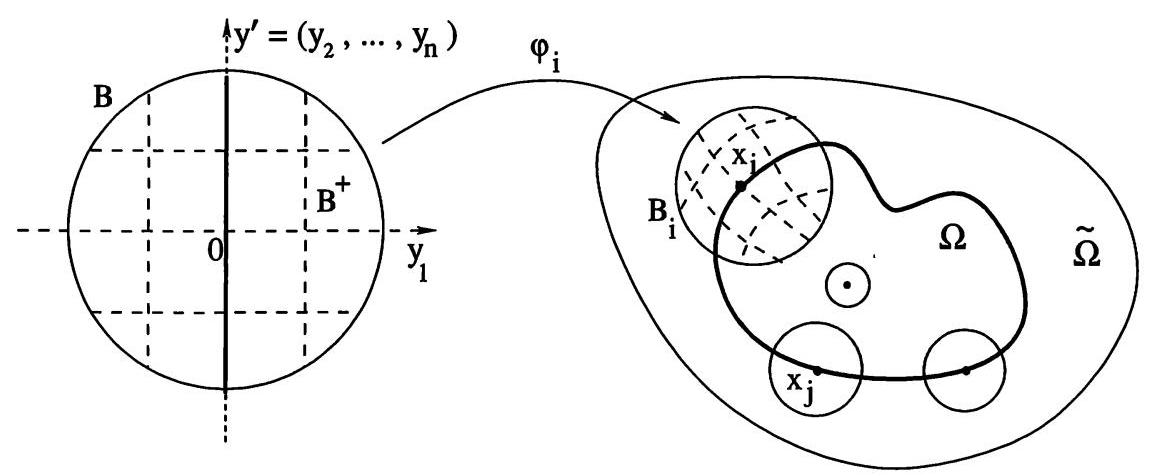
\includegraphics[width=1.0\textwidth]{images/bo_d6ik6nn7aajc739ct1l0_174_168_582_1149_476_0.jpg}
\caption{集合 $\Omega$ 的开覆盖.对每个球 ${B}_{i} = \; B\left( {{x}_{i},{r}_{i}}\right)$ ，存在一个 ${\mathcal{C}}^{1}$ 双射 ${\varphi }_{i}$ ，将单位开球 $B \subset  {\mathbb{R}}^{n}$ 映射到 ${B}_{i}$ .对那些以边界 $\Omega$ 上点为球心的球 ${B}_{i}$ ，正半球 ${B}^{ + } = B \cap  \left\{  {{y}_{1} > 0}\right\}$ 被映射到交集 ${B}_{i} \cap  \Omega$ .}
\label{fig:omega-covering}
\end{figure}

\noindent 2. 为处理一般情形，我们使用单位分解.对每个 $x \in  \overline{\Omega }$ (即 $\Omega$ 的闭包)，选取半径 ${r}_{x} > 0$ ，使得以 $x$ 为中心、半径为 ${r}_{x}0$ 的开球 $B\left( {x,{r}_{x}}\right)$ 满足以下条件:
\begin{itemize}
\item 若 $x \in  \Omega$ ，则 $B\left( {x,{r}_{x}}\right)  \subset  \Omega$ .
\item 若 $x \in  \partial \Omega$ ，则 $B\left( {x,{r}_{x}}\right)  \subset  \widetilde{\Omega }$ .此外，记 $B \doteq  B\left( {0,1}\right)$ 为 ${\mathbb{R}}^{n}$ 中的单位开球，则存在一个 ${\mathcal{C}}^{1}$ 双射 ${\varphi }^{x} : B \mapsto  B\left( {x,{r}_{x}}\right)$ ，其逆映射亦为 ${\mathcal{C}}^{1}$ ，该映射将半球
\[
{B}^{ + } \doteq  \left\{  {y = \left( {{y}_{1},{y}_{2},\ldots ,{y}_{n}}\right) ;\sum_{{i = 1}}^{n}{y}_{i}^{2} < 1,{y}_{1} > 0}\right\}
\]
映射到集合 $B\left( {x,{r}^{x}}\right)  \cap  \Omega$ .
\end{itemize}


当 ${r}_{x} > 0$ 取得足够小时，此类双射的存在性由 $\Omega$ 具有 ${\mathcal{C}}^{1}$ 边界的假设保证.

由于 $\Omega$ 有界，其闭包 $\overline{\Omega }$ 是紧的，故可被有限个球 ${B}_{i} = B\left( {{x}_{i},{r}_{i}}\right) ,i = 1,\ldots ,N$ 覆盖.设 ${\varphi }_{i} : B \mapsto  {B}_{i}$ 为对应的双射.回顾可知 ${\varphi }_{i}$ 将 ${B}^{ + }$ 映射到 ${B}_{i} \cap  \Omega$ .

\noindent 3. 设 ${\eta }_{1},\ldots ,{\eta }_{N}$ 为上述覆盖的光滑单位分解.对每个 $x \in  \Omega$ ，我们有
\begin{equation}\tag{8.41}\label{eq:partition-unity-u}
u\left( x\right)  = \sum_{{i = 1}}^{N}{\eta }_{i}\left( x\right) u\left( x\right) .
\end{equation}

我们将指标集划分为
\[
\{ 1,2,\ldots ,N\}  = \mathcal{I} \cup  \mathcal{J},
\]
其中 $\mathcal{I}$ 包含满足 ${x}_{i} \in  \Omega$ 的指标，而 $\mathcal{J}$ 包含满足 ${x}_{i} \in  \partial \Omega$ 的指标.

对每个 $i \in  \mathcal{J}$ ，有 ${\eta }_{i}u \in  {W}^{1,p}\left( {{B}_{i} \cap  \Omega }\right)$ .因此由定理\ref{thm:weak-derivative-properties}(iv)得 $\left( {{\eta }_{i}u}\right)  \circ  {\varphi }_{i} \in  {W}^{1,p}\left( {B}^{ + }\right)$ .应用在\eqref{eq:extension-reflection}处定义的延拓算子 ${E}^{\sharp }$ ，得到
\[
{E}^{\sharp }\left( {\left( {{\eta }_{i}u}\right)  \circ  {\varphi }_{i}}\right) \; \in  \;{W}^{1,p}\left( {B}^{ + }\right) ,\;{E}^{\sharp }\left( {\left( {{\eta }_{i}u}\right)  \circ  {\varphi }_{i}}\right)  \circ  {\varphi }_{i}^{-1}\; \in  \;{W}^{1,p}\left( {B}_{i}\right) .
\]

将所有这些延拓相加，我们定义
\[
{Eu} \doteq  \sum_{{i \in  \mathcal{I}}}{\eta }_{i}u + \sum_{{i \in  \mathcal{J}}}{E}^{\sharp }\left( {\left( {{\eta }_{i}u}\right)  \circ  {\varphi }_{i}}\right)  \circ  {\varphi }_{i}^{-1}.
\]

现在显然，延拓算子 $E$ 满足所有要求.事实上，(i)由\eqref{eq:partition-unity-u}推出；性质(ii)源于如下事实:对每个 $u \in  {W}^{1,p}\left( \Omega \right)$ ， ${Eu}$ 的支集包含于 $\mathop{\bigcup }\limits_{{i = 1}}^{N}{B}_{i} \subseteq  \widetilde{\Omega }$ ；最后，由于 $E$ 被定义为有限个有界线性算子之和，故存在某个常数 $C$ ，使得估计式(iii)成立.

\end{proof}

\section{嵌入定理}

在一维空间中，若函数 $u : \mathbb{R} \mapsto  \mathbb{R}$ 存在弱导数 ${Du} \in  {L}^{1}\left( \mathbb{R}\right)$ ，则其(在零测集上修改取值后)绝对连续；反之，若 $\Omega  \subseteq  {\mathbb{R}}^{n}$ 且 $n \geq  2$ ，则存在既不连续也不有界的函数 $u \in  {W}^{1,p}\left( \Omega \right)$ .例如函数 $u\left( x\right)  = {\left| x\right| }^{-\gamma }$ 在 $0 < \gamma  < \frac{n - p}{p}$ 时即属此情形.

在偏微分方程或变分法的诸多应用中，理解函数 $u \in \; {W}^{k,p}\left( {\mathbb{R}}^{n}\right)$ 所具有的正则性程度至关重要.我们将证明两个朝此方向的基本结果.

\noindent 1.(Morrey)若 $p > n$ ，则每个函数 $u \in  {W}^{1,p}\left( {\mathbb{R}}^{n}\right)$ (在零测集上修改后)均Hölder连续.

\noindent 2.(Gagliardo-Nirenberg)若 $p < n$ ，则每个函数 $u \in  {W}^{1,p}\left( {\mathbb{R}}^{n}\right)$ 属于空间 ${L}^{{p}^{ * }}\left( {\mathbb{R}}^{n}\right)$ ，且具有更大的指数 ${p}^{ * } = p + \frac{{p}^{2}}{n - p}$ .

在这两种情形下，结果均可表述为嵌入定理:在零测集上修改后，每个函数 $u \in  {W}^{1,p}\left( \Omega \right)$ 亦属于某个其他Banach空间 $X$ ；此处 $X = {C}^{0,\gamma }$ 或 $X = {L}^{q}$ ，其中 $q > p$ 为某常数.基本思路如下:
\begin{enumerate}[(I)]
    \item \allbf{对所有光滑函数证明先验估计.}对任意函数 $u \in  {\mathcal{C}}^{\infty }\left( \Omega \right)  \cap  {W}^{k,p}\left( \Omega \right)$ ，证明 $u$ 亦属于另一Banach空间 $X$ ，且存在仅依赖于 $k,p,\Omega$ 而与 $u$ 无关的常数 $C$ ，使得
\begin{equation}\tag{8.42}\label{eq:embedding-apriori}
\| u{\| }_{X}\; \leq  \;C\| u{\| }_{{W}^{k,p}}\;\forall\,u \in  {\mathcal{C}}^{\infty }\left( \Omega \right)  \cap  {W}^{k,p}\left( \Omega \right) \;.
\end{equation}
    \item \allbf{利用连续性将嵌入推广至整个空间.}由于 ${\mathcal{C}}^{\infty }$ 在 ${W}^{k,p}$ 中稠密，故对每个 $u \in  {W}^{k,p}\left( \Omega \right)$ ，可找到一列函数 ${u}_{n} \in  {\mathcal{C}}^{\infty }\left( \Omega \right)$ 使得 $\norm{u - {u}_{n}}_{{W}^{k,p}} \rightarrow  0$ 成立.由\eqref{eq:embedding-apriori}式，
    \[
    \limsup_{{m,n \rightarrow  \infty }}{\norm{u_{m} - {u}_{n}}}_{X} \leq  \limsup_{{m,n \rightarrow  \infty }}C{\norm{u_{m} - {u}_{n}}}_{{W}^{k,p}} = 0.
    \]
    因此，函数 ${u}_{n}$ 在空间 $X$ 中也构成Cauchy列.由完备性可知， ${u}_{n} \rightarrow  \widetilde{u}$ 对某个 $\widetilde{u} \in  X$ 成立.注意到对几乎处处的 $x \in  \Omega$ 有 $\widetilde{u}\left( x\right)  = u\left( x\right)$ ，故可推出:在测度为零的集合 $\mathcal{N} \subset  \Omega$ 上作适当修改后，每个函数 $u \in  {W}^{k,p}\left( \Omega \right)$ 也属于空间 $X$ .
\end{enumerate}



\subsection{莫雷不等式}

本节证明:若 $u \in  {W}^{1,p}\left( {\mathbb{R}}^{n}\right)$ ，其中指数 $p$ 大于空间维数 $n$ ，则 $u$ 几乎处处等于一个Hölder连续函数.
\begin{theorem}[莫雷不等式]\label{thm:morrey-inequality}
设 $n < p < \infty$ ，并令 $\gamma  \doteq  1 - \frac{n}{p} > 0$ .则存在仅依赖于 $p$ 和 $n$ 的常数 $C$ ，使得
\begin{equation}\tag{8.43}\label{eq:morrey-inequality}
\| u{\| }_{{\mathcal{C}}^{0,\gamma }\left( {\mathbb{R}}^{n}\right) }\; \leq  \;C\| u{\| }_{{W}^{1,p}\left( {\mathbb{R}}^{n}\right) }
\end{equation}

对每个 $u \in  {\mathcal{C}}^{1}\left( {\mathbb{R}}^{n}\right)  \cap  {W}^{1,p}\left( {\mathbb{R}}^{n}\right)$ 成立.
\end{theorem}

\begin{proof}
在给出严格证明之前，先概述其思想.由函数$u$的梯度满足的一个积分估计，例如
\begin{equation}\tag{8.44}\label{eq:morrey-gradient-Lp-bound}
{\int }_{{\mathbb{R}}^{n}}{\left| \nabla u\left( x\right) \right| }^{p}{\d x} \leq  {C}_{0}
\end{equation}
我们希望得到如下形式的逐点估计:
\begin{equation}\tag{8.45}\label{eq:morrey-holder-target}
\left| {u\left( y\right)  - u\left( {y}^{\prime }\right) }\right|  \leq  {C}_{1}{\left| y - {y}^{\prime }\right| }^{\gamma }\;\forall\,y,{y}^{\prime } \in  {\mathbb{R}}^{n}.
\end{equation}

\begin{figure}[htbp]
\centering
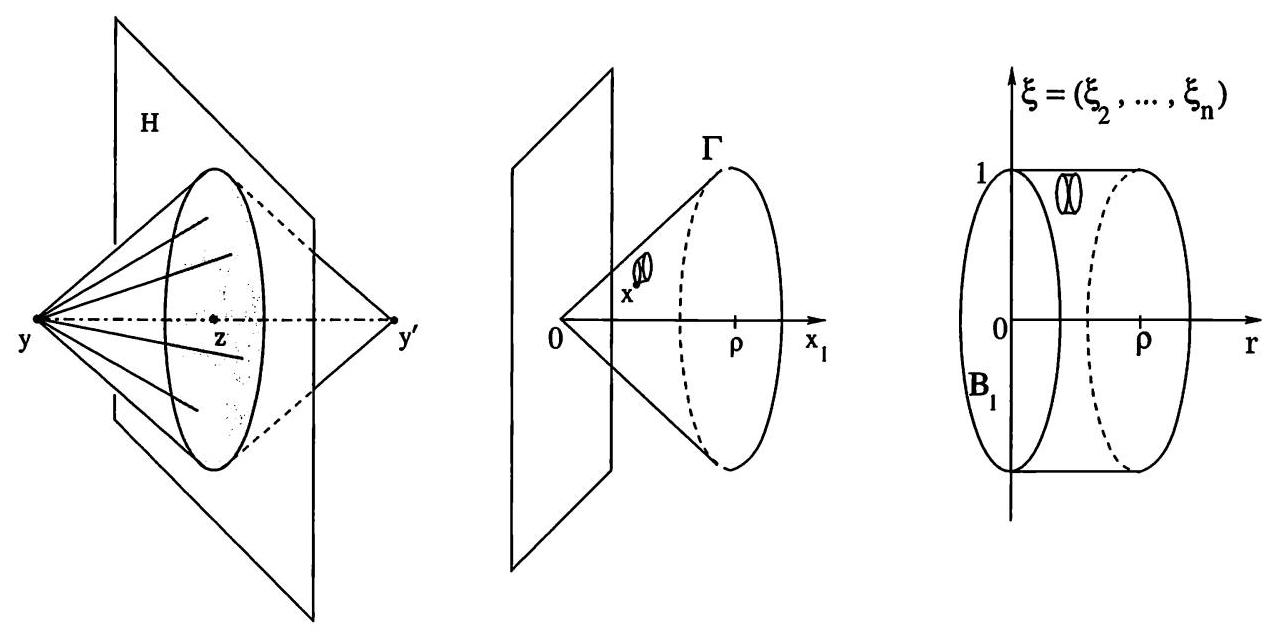
\includegraphics[width=0.95\textwidth]{images/bo_d6ik6nn7aajc739ct1l0_177_106_234_1282_634_0.jpg}
\caption{莫雷不等式的证明.左:在垂直于向量 $y - {y}^{\prime }$ 的超平面 $H$ 内，以中点 $z$ 为中心、位于该平面内的 $\left( {n - 1}\right)$ 维球(阴影区域)上取函数 $u$ 的平均值，并将 $u\left( y\right)$ 与 $u\left( {y}^{\prime }\right)$ 的值分别与之比较.中与右:锥 $\Gamma$ 中一点 $x$ 用坐标 $\left( {r,\xi }\right)  \in  \left(  {0,\rho }\right)   \times  {B}_{1}$ 表示.}
\label{fig:morrey-proof}
\end{figure}

为实现\eqref{eq:morrey-holder-target}，一种自然尝试是写作
\begin{equation}\tag{8.46}\label{eq:morrey-segment-bound}
    \setjot[-2]\begin{aligned}
        \left| {u\left( y\right)  - u\left( {y}^{\prime }\right) }\right|  &= \left| {{\int }_{0}^{1}\left(  {\frac{d}{d\theta }u\left( {{\theta y} + \left( {1 - \theta }\right) {y}^{\prime }}\right) }\right)  {d\theta }}\right|\\
        &\leq  {\int }_{0}^{1}\left| {\nabla u\left( {{\theta y} + \left( {1 - \theta }\right) {y}^{\prime }}\right) }\right| \left| {y - {y}^{\prime }}\right| {d\theta }.
    \end{aligned}
\end{equation}

然而，\eqref{eq:morrey-segment-bound}式右端积分仅涉及 $\nabla u$ 在连接 $y$ 与 ${y}^{\prime }$ 的线段上的取值.若空间维数为 $n > 1$ ，则该线段测度为零；因此即使\eqref{eq:morrey-gradient-Lp-bound}中的积分很小，\eqref{eq:morrey-segment-bound}式右端积分仍可能任意大.为克服这一困难，我们将 $u\left( y\right) ,u\left( {y}^{\prime }\right)$ 二者均与函数 $u$ 在以中点 $z = \frac{y + {y}^{\prime }}{2}$ 为中心的 $\left( {n - 1}\right)$ 维球上的平均值 ${u}_{A}$ 进行比较，如图\ref{fig:morrey-proof}(左)所示.注意，差值 $\left| {u\left( y\right)  - {u}_{A}}\right|$ 可通过在 $n$ 维锥上对 $\left| {\nabla u}\right|$ 积分来估计.由此便可利用界\eqref{eq:morrey-gradient-Lp-bound}.

\noindent 1. 现在开始证明，并先作一预备计算.在 ${\mathbb{R}}^{n}$ 上考虑锥
\[
\Gamma  \doteq  \left\{  {x = \left( {{x}_{1},{x}_{2},\ldots ,{x}_{n}}\right) ;\;\sum_{{j = 2}}^{n}{x}_{j}^{2} \leq  {x}_{1}^{2},\;0 < {x}_{1} < \rho }\right\}
\]
及函数
\begin{equation}\tag{8.47}\label{eq:morrey-psi}
\psi \left( x\right)  = \frac{1}{{x}_{1}^{n - 1}}.
\end{equation}

令 $q = \frac{p}{p - 1}$ 为 $p$ 的共轭指数，即满足 $\frac{1}{p} + \frac{1}{q} = 1$ .我们计算
{\setjot[0]\begin{align*}
    \| \psi {\| }_{{L}^{q}\left( \Gamma \right) }^{q} &= {\int }_{\Gamma }{\left( \frac{1}{{x}_{1}^{n - 1}}\right) }^{q}{\d x} = {\int }_{0}^{\rho }{c}_{n - 1}{x}_{1}^{n - 1}{\left( \frac{1}{{x}_{1}^{n - 1}}\right) }^{q}\d x_{1}\\
    &= {c}_{n - 1}{\int }_{0}^{\rho }{s}^{\left( {n - 1}\right) \left( {1 - q}\right) }{\d s}
\end{align*}}
其中常数 ${c}_{n - 1}$ 给出 ${\mathbb{R}}^{n - 1}$ 中单位球的体积.因此， $\psi  \in  {L}^{q}\left( \Gamma \right)$ 当且仅当 $n < p$ .此时，
\begin{equation}\tag{8.48}\label{eq:morrey-psi-norm}
\| \psi {\| }_{{L}^{q}\left( \Gamma \right) } = {\left( {c}_{n - 1}{\int }_{0}^{\rho }{s}^{-\frac{n - 1}{p - 1}}\d s\right) }^{\frac{1}{q}} = c{\left( {\rho }^{\frac{p - n}{p - 1}}\right) }^{\frac{p - 1}{p}} = c{\rho }^{\frac{p - n}{p}},
\end{equation}
其中常数 $c$ 仅依赖于 $n$ 和 $p$ .

\noindent 2. 考虑任意两个不同点 $y,{y}^{\prime } \in  {\mathbb{R}}^{n}$ .令 $\rho  \doteq  \frac{1}{2}\left| {y - {y}^{\prime }}\right|$ .过中点 $z \doteq  \frac{y + {y}^{\prime }}{2}$ 且垂直于向量 $y - {y}^{\prime }$ 的超平面方程为
\[
H = \left\{  {x \in  {\mathbb{R}}^{n};\left\langle  {x - z,y - {y}^{\prime }}\right\rangle   = 0}\right\}  .
\]

在 $H$ 内，考虑以 $z$ 为中心、半径为 $\rho$ 的 $\left( {n - 1}\right)$ 维球，
\[
{B}_{\rho } \doteq  \{ x \in  H;\left| {x - z}\right|  < \rho \} .
\]

记 ${u}_{A}$ 为 $u$ 在球 ${B}_{\rho }$ 上的平均值，则差值 $\left| {u\left( y\right)  - u\left( {y}^{\prime }\right) }\right|$ 将被估计为
\begin{equation}\tag{8.49}\label{eq:morrey-split}
\left| {u\left( y\right)  - u\left( {y}^{\prime }\right) }\right|  \leq  \left| {u\left( y\right)  - {u}_{A}}\right|  + \left| {{u}_{A} - u\left( {y}^{\prime }\right) }\right| .
\end{equation}

\noindent 3. 通过坐标平移与旋转，可假设
\[
y = \left( {0,\ldots ,0}\right)  \in  {\mathbb{R}}^{n},\;\quad {B}_{\rho } = \left\{  {x = \left( {{x}_{1},{x}_{2},\ldots ,{x}_{n}}\right) ;{x}_{1} = \rho ,\sum_{{i = 2}}^{n}{x}_{i}^{2} \leq  {\rho }^{2}}\right\}  .
\]

为计算平均值 ${u}_{A}$ ，令 ${B}_{1}$ 为 ${\mathbb{R}}^{n - 1}$ 中的单位球，并令 ${c}_{n - 1}$ 为其 $\left( {n - 1}\right)$ 维测度.锥体 $\Gamma$ 中的点将用另一套坐标系描述.对具有坐标 $\left( {r,\xi }\right)  = \left( {r,{\xi }_{2},\ldots ,{\xi }_{n}}\right)  \in  \left(  {0,\rho }\right)   \times  {B}_{1}$ 的点，关联其具有分量的点 $x\left( {r,\xi }\right)  \in  \Gamma$
\begin{equation}\tag{8.50}\label{eq:morrey-cone-coords}
\left( {{x}_{1},{x}_{2},\ldots ,{x}_{n}}\right)  = \left( {r,{r\xi }}\right)  = \left( {r,r{\xi }_{2},\ldots ,r{\xi }_{n}}\right) .
\end{equation}

定义 $U\left( {r,\xi }\right)  = u\left( {r,{r\xi }}\right)$ ，并注意到对每个 $\xi$ 均有 $U\left( {0,\xi }\right)  = u\left( 0\right)$ .

因此
\[
U\left( {\rho ,\xi }\right)  = U\left( {0,\xi }\right)  + {\int }_{0}^{\rho }\left(  {\frac{\partial }{\partial r}U\left( {r,\xi }\right) }\right)  {\d r},
\]
\begin{equation}\tag{8.51}\label{eq:morrey-uA-average}
{u}_{A} - u\left( 0\right)  = \frac{1}{{c}_{n - 1}}{\int }_{{B}_{1}}\left( {{\int }_{0}^{\rho }\left(  {\frac{\partial }{\partial r}U\left( {r,\xi }\right) }\right)  {\d r}}\right) {\d \xi }.
\end{equation}

我们现在作变量替换，将积分\eqref{eq:morrey-uA-average}在 $\left(  {0,\rho }\right)   \times  {B}_{1}$ 上的积分变换为在锥体 $\Gamma$ 上的积分.计算变换\eqref{eq:morrey-cone-coords}的雅可比矩阵，得其行列式为 ${r}^{n - 1}$ ；故
\[
\d x_{1}\d x_{2}\cdots \d x_{n} = {r}^{n - 1}\d{r}\d{\xi }_{2}\cdots \d{\xi }_{n}.
\]

此外，由于 $\left| \xi \right|  \leq  1$ ，函数 $u$ 沿向量 $\left( {1,{\xi }_{2},\ldots ,{\xi }_{n}}\right)$ 方向的方向导数被估计为
\begin{equation}\tag{8.52}\label{eq:morrey-dUr-bound}
\left| {\frac{\partial }{\partial r}U\left( {r,\xi }\right) }\right|  = \left| {{u}_{{x}_{1}} + \sum_{{i = 2}}^{n}{\xi }_{i}{u}_{{x}_{i}}}\right|  \leq  2\left| {\nabla u\left( {r,\xi }\right) }\right| .
\end{equation}

在\eqref{eq:morrey-uA-average}中代入\eqref{eq:morrey-dUr-bound}，并利用函数 $\psi \left( x\right)  \doteq  {x}_{1}^{1 - n}$ 的 ${L}^{q}$ 范数估计\eqref{eq:morrey-psi-norm}，得到
\begin{equation}\tag{8.53}\label{eq:morrey-uA-bound}
    {\setjot[0]\begin{aligned}
        \left| {{u}_{A} - u\left( 0\right) }\right|  &\leq  \frac{2}{{c}_{n - 1}}{\int }_{\Gamma }\frac{1}{{x}_{1}^{n - 1}}\left| {\nabla u\left( x\right) }\right| {\d x}\\
        &\leq  \frac{2}{{c}_{n - 1}}\| \psi {\| }_{{L}^{q}\left( \Gamma \right) }\| \nabla u{\| }_{{L}^{p}\left( \Gamma \right) }\;\quad \left( {q = \frac{p}{p - 1}}\right)\\
        &\leq  C{\rho }^{\frac{p - n}{p}}\| u{\| }_{{W}^{1,p}\left( {\mathbb{R}}^{n}\right) }.
    \end{aligned}}
\end{equation}
其中 $C$ 为某常数.注意最后两步分别由 Hölder 不等式及\eqref{eq:morrey-psi-norm}得出.

\noindent 4. 利用\eqref{eq:morrey-uA-bound}估计\eqref{eq:morrey-split}右端每一项，并回顾 $\rho  = \frac{1}{2}\left| {y - {y}^{\prime }}\right|$ ，我们得出
\begin{equation}\tag{8.54}\label{eq:morrey-holder}
\left| {u\left( y\right)  - u\left( {y}^{\prime }\right) }\right|  \leq  {2C}{\left( \frac{\left| y - {y}^{\prime }\right| }{2}\right) }^{\frac{p - n}{p}}\| u{\| }_{{W}^{1,p}\left( {\mathbb{R}}^{n}\right) }.
\end{equation}

这表明 $u$ 是指数为 $\gamma  = \frac{p - n}{p}$ 的 Hölder 连续函数.

\noindent 5. 为估计 $\mathop{\sup }\limits_{y}\left| {u\left( y\right) }\right|$ ，我们注意到，由\eqref{eq:morrey-holder}，存在某常数 ${C}_{1}$ ，使得
\[
\left| {u\left( y\right) }\right|  \leq  \left| {u\left( x\right) }\right|  + {C}_{1}\| u{\| }_{{W}^{1,p}\left( {\mathbb{R}}^{n}\right) }\;\forall\,x \in  B\left( {y,1}\right) .
\]

对以 $y$ 为中心、半径为1的球上右侧表达式取平均，得到
\begin{equation}\tag{8.55}\label{eq:morrey-sup-estimate}
\left| {u\left( y\right) }\right|  \leq  {\int }_{B\left( {y,1}\right) }\left| {u\left( x\right) }\right| {\d x} + {C}_{1}\| u{\| }_{{W}^{1,p}\left( {\mathbb{R}}^{n}\right) } \leq  {C}_{2}\| u{\| }_{{L}^{p}\left( {\mathbb{R}}^{n}\right) } + {C}_{1}\| u{\| }_{{W}^{1,p}\left( {\mathbb{R}}^{n}\right) }.
\end{equation}

\noindent 6. 综合\eqref{eq:morrey-holder}--\eqref{eq:morrey-sup-estimate}可得
\[
\| u{\| }_{{\mathcal{C}}^{0,\gamma }\left( {\mathbb{R}}^{n}\right) } \doteq  \mathop{\sup }\limits_{y}\left| {u\left( y\right) }\right|  + \mathop{\sup }\limits_{{y \neq  {y}^{\prime }}}\frac{\left| u\left( y\right)  - u\left( {y}^{\prime }\right) \right| }{{\left| y - {y}^{\prime }\right| }^{\gamma }} \leq  C\| u{\| }_{{W}^{1,p}\left( {\mathbb{R}}^{n}\right) },
\]
其中常数 $C$ 仅依赖于 $p$ 和 $n$ .
\end{proof}

由于 ${\mathcal{C}}^{\infty }$ 在 ${W}^{1,p}$ 中稠密，由定理\ref{thm:morrey-inequality}可得

\begin{corollary}[嵌入]\label{cor:morrey-embedding}
设 $\Omega  \subset  {\mathbb{R}}^{n}$ 为具有 ${\mathcal{C}}^{1}$ 边界的有界开集.假设 $n < p < \infty$ ，并令 $\gamma  \doteq  1 - \frac{n}{p} > 0$ .则每个函数 $f \in  {W}^{1,p}\left( \Omega \right)$ 几乎处处等于某个函数 $\widetilde{f} \in  {\mathcal{C}}^{0,\gamma }\left( \Omega \right)$ .此外，存在常数 $C$ ，使得
\begin{equation}\tag{8.56}\label{eq:morrey-embedding}
\| \widetilde{f}{\| }_{{\mathcal{C}}^{0,\gamma }} \leq  C\| f{\| }_{{W}^{1,p}}\;\forall\,f \in  {W}^{1,p}\left( \Omega \right) .
\end{equation}
\end{corollary}

\begin{proof}
1. 令 $\widetilde{\Omega } \doteq  \left\{  {x \in  {\mathbb{R}}^{n};d\left( {x,\Omega }\right)  < 1}\right\}$ 为集合 $\Omega$ 的半径为1的开邻域.由定理\ref{thm:extension-operator}可知，存在有界延拓算子 $E$ ，它将每个函数 $f \in  {W}^{1,p}\left( \Omega \right)$ 延拓为支集包含于 $\widetilde{\Omega }$ 内的函数 ${Ef} \in  {W}^{1,p}\left( {\mathbb{R}}^{n}\right)$ .

\noindent 2. 由于 ${\mathcal{C}}^{1}\left( {\mathbb{R}}^{n}\right)$ 在 ${W}^{1,p}\left( {\mathbb{R}}^{n}\right)$ 中稠密，可取一列函数 ${g}_{n} \in  {\mathcal{C}}^{1}\left( {\mathbb{R}}^{n}\right)$ 在 ${W}^{1,p}\left( {\mathbb{R}}^{n}\right)$ 中收敛于 ${Ef}$ .由定理\ref{thm:morrey-inequality}
\[
\limsup_{{m,n \rightarrow  \infty }}{\norm{g_{m} - {g}_{n}}}_{{C}^{0,\gamma }\left( {\mathbb{R}}^{n}\right) } \leq  C\limsup_{{m,n \rightarrow  \infty }}{\norm{g_{m} - {g}_{n}}}_{{W}^{1,p}\left( {\mathbb{R}}^{n}\right) } = 0.
\]

这表明序列 ${\left( {g}_{n}\right) }_{n \geq  1}$ 在空间 ${\mathcal{C}}^{0,\gamma }$ 中亦为Cauchy列.因此它一致收敛于某个极限函数 $g \in  {C}^{0,\gamma }\left( {\mathbb{R}}^{n}\right)$ (对 $x \in  {\mathbb{R}}^{n}$ 一致).

\noindent 3. 由于 ${g}_{n} \rightarrow  {Ef}$ 在 ${W}^{1,p}\left( {\mathbb{R}}^{n}\right)$ 中，故对$\text{a.e.}\; x \in  {\mathbb{R}}^{n}$ 亦有 $g\left( x\right)  = \left( {Ef}\right) \left( x\right)$ .特别地，对$\text{a.e.}\;x \in  \Omega$ 有 $g\left( x\right)  = f\left( x\right)$ .又因延拓算子 $E$ 有界，由式\eqref{eq:morrey-inequality}可推出\eqref{eq:morrey-embedding}.
\end{proof}

\begin{remark}\label{rem:morrey-embedding-Rn}
若 $\Omega  = {\mathbb{R}}^{n}$ ，推论\ref{cor:morrey-embedding}的结论仍成立.
\end{remark}

\subsection{Gagliardo--Nirenberg不等式}

接下来我们研究 $1 \leq  p < n$ 的情形.定义 $p$ 的\bluebf{Soblev共轭}为
\begin{equation}\tag{8.57}\label{eq:p-star}
{p}^{ * } \doteq  \frac{np}{n - p} > p.
\end{equation}

注意， ${p}^{ * }$ 不仅依赖于 $p$ ，还依赖于空间的维数 $n$ :
\begin{equation}\tag{8.58}\label{eq:p-star-reciprocal}
\frac{1}{{p}^{ * }} = \frac{1}{p} - \frac{1}{n}
\end{equation}

作为预备知识，我们介绍广义Hölder不等式的一个有用应用；参见附录中的(A.26).设给定非负函数 $n - 1$  ${g}_{1},{g}_{2},\ldots ,{g}_{n - 1} \in  {L}^{1}\left( \Omega \right)$ .由于对每个 $i$ 均有 ${g}_{i}^{\frac{1}{n - 1}} \in  {L}^{n - 1}\left( \Omega \right)$，应用广义Hölder不等式可得
\begin{equation}\tag{8.59}\label{eq:generalized-holder-application}
{\int }_{\Omega }{g}_{1}^{\frac{1}{n - 1}}{g}_{2}^{\frac{1}{n - 1}}\cdots {g}_{n - 1}^{\frac{1}{n - 1}}{\d s} \leq  \mathop{\prod }\limits_{{i = 1}}^{{n - 1}}{\norm{g_{i}^{\frac{1}{n - 1}}}}_{{L}^{n - 1}} = \mathop{\prod }\limits_{{i = 1}}^{{n - 1}}{\norm{g}_{i}}_{{L}^{1}}^{\frac{1}{n - 1}}.
\end{equation}

\begin{theorem}[Gagliardo--Nirenberg不等式]\label{thm:gagliardo-nirenberg}
假设 $1 \leq  p < n$ .则存在仅依赖于 $p$ 和 $n$ 的常数 $C$ ，使得
\begin{equation}\tag{8.60}\label{eq:gagliardo-nirenberg}
\| f{\| }_{{L}^{{p}^{ * }}\left( {\mathbb{R}}^{n}\right) }\; \leq  \;C\| \nabla f{\| }_{{L}^{p}\left( {\mathbb{R}}^{n}\right) },\;\forall\,\;f \in  {C}_{c}^{1}\left( {\mathbb{R}}^{n}\right) .
\end{equation}
\end{theorem}

\begin{figure}[htbp]
\centering
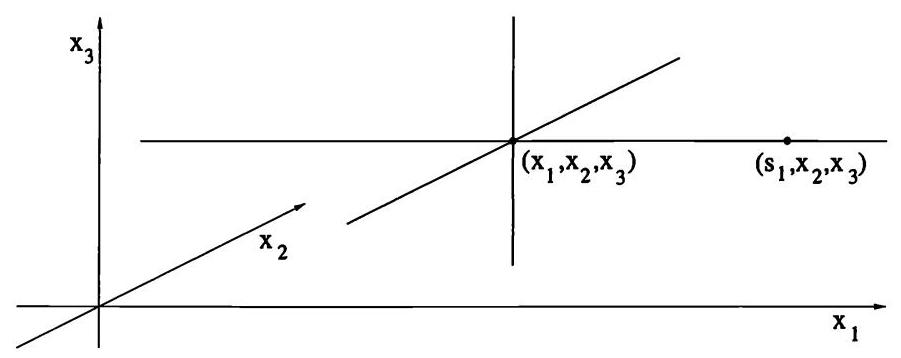
\includegraphics[width=0.8\textwidth]{images/bo_d6ik6nn7aajc739ct1l0_181_291_1364_901_358_0.jpg}
\caption{证明加利亚尔多--尼伦伯格不等式.积分 ${\int }_{-\infty }^{\infty }\left| {{D}_{{x}_{1}}f\left( {{s}_{1},{x}_{2},{x}_{3}}\right) }\right| \d s_{1}$ 依赖于 ${x}_{2},{x}_{3}$ 但不依赖于 ${x}_{1}$ .类似地，积分 ${\int }_{-\infty }^{\infty }\left| {{D}_{{x}_{2}}f\left( {{x}_{1},{s}_{2},{x}_{3}}\right) }\right| \d s_{2}$ 依赖于 ${x}_{1},{x}_{3}$ 但不依赖于 ${x}_{2}$ .}
\label{fig:gn-proof}
\end{figure}

\begin{proof}
1. 对每个 $i \in  \{ 1,\ldots ,n\}$ 及每一点 $x = \left( {{x}_{1},\ldots ,{x}_{i},\ldots ,{x}_{n}}\right)  \in \; {\mathbb{R}}^{n}$ ，由于 $f$ 具有紧支集，可写为
\[
f\left( {{x}_{1},\ldots ,{x}_{i},\ldots ,{x}_{n}}\right)  = {\int }_{-\infty }^{{x}_{i}}{D}_{{x}_{i}}f\left( {{x}_{1},\ldots ,{s}_{i},\ldots ,{x}_{n}}\right) \d s_{i}.
\]

进而得到
\[
\left| {f\left( {{x}_{1},\ldots ,{x}_{n}}\right) }\right|  \leq  {\int }_{-\infty }^{\infty }\left| {{D}_{{x}_{i}}f\left( {{x}_{1},\ldots ,{s}_{i},\ldots ,{x}_{n}}\right) }\right| \d s_{i},\;1 \leq  i \leq  n,
\]
\begin{equation}\tag{8.61}\label{eq:gn-pointwise}
{\left| f\left( x\right) \right| }^{\frac{n}{n - 1}} \leq  \mathop{\prod }\limits_{{i = 1}}^{n}{\left( {\int }_{-\infty }^{\infty }\left| {D}_{{x}_{i}}f\left( {x}_{1},\ldots ,{s}_{i},\ldots ,{x}_{n}\right) \right| \d s_{i}\right) }^{\frac{1}{n - 1}}.
\end{equation}

现对\eqref{eq:gn-pointwise}关于 ${x}_{1}$ 积分.注意右侧第一因子不依赖于 ${x}_{1}$ .该因子表现如常数，可提出积分号外.剩余 $n - 1$ 个因子的乘积则利用\eqref{eq:generalized-holder-application}处理.由此得到\eqref{eq:gn-integrate-x1}
\begin{equation}\tag{8.62}\label{eq:gn-integrate-x1}
\begin{aligned}
&{\int }_{-\infty }^{\infty }{\left| f\right| }^{\frac{n}{n - 1}}\d x_{1}\\
&\leq  {\left( {\int }_{-\infty }^{\infty }\left| {D}_{{x}_{1}}f\right| \d s_{1}\right) }^{\frac{1}{n - 1}}{\int }_{-\infty }^{\infty }\mathop{\prod }\limits_{{i = 2}}^{n}{\left( {\int }_{-\infty }^{\infty }\left| {D}_{{x}_{i}}f\right| \d s_{i}\right) }^{\frac{1}{n - 1}}\d x_{1} \\
&\leq  {\left( {\int }_{-\infty }^{\infty }\left| {D}_{{x}_{1}}f\right| \d s_{1}\right) }^{\frac{1}{n - 1}}\mathop{\prod }\limits_{{i = 2}}^{n}{\left( {\int }_{-\infty }^{\infty }{\int }_{-\infty }^{\infty }\left| {D}_{{x}_{i}}f\right| \d s_{i}\d x_{1}\right) }^{\frac{1}{n - 1}}.
\end{aligned}
\end{equation}
注意第二个不等式是将广义Hölder不等式应用于 $n - 1$ 个函数 ${g}_{i} = {\int }_{-\infty }^{\infty }\left| {{D}_{{x}_{i}}f}\right| \d s_{i},i = 2,\ldots ,n$ 所得.

现对\eqref{eq:gn-integrate-x1}两边关于 ${x}_{2}$ 积分.注意\eqref{eq:gn-integrate-x1}右侧乘积中出现的一个因子不依赖于变量 ${x}_{2}$ (即涉及关于 ${s}_{2}$ 积分的那个因子).该因子表现如常数，可提出积分号外.剩余 $n - 2$ 个因子的乘积再次用Hölder不等式估计.由此得到
\begin{equation}\tag{8.63}\label{eq:gn-integrate-x2}
\begin{aligned}
&{\int }_{-\infty }^{\infty }{\int }_{-\infty }^{\infty }{\left| f\right| }^{\frac{n}{n - 1}}\d x_{1}\d x_{2}\\
&\leq  {\left( {\int }_{-\infty }^{\infty }{\int }_{-\infty }^{\infty }\left| {D}_{{x}_{1}}f\right| \d x_{1}\d x_{2}\right) }^{\frac{1}{n - 1}}{\left( {\int }_{-\infty }^{\infty }{\int }_{-\infty }^{\infty }\left| {D}_{{x}_{2}}f\right| \d x_{1}\d x_{2}\right) }^{\frac{1}{n - 1}} \\
&\quad\times  \mathop{\prod }\limits_{{i = 3}}^{n}{\left( {\int }_{-\infty }^{\infty }{\int }_{-\infty }^{\infty }{\int }_{-\infty }^{\infty }\left| {D}_{{x}_{i}}f\right| \d s_{i}\d x_{1}\d x_{2}\right) }^{\frac{1}{n - 1}}.
\end{aligned}
\end{equation}

依同样方式继续，经过 $n$ 次积分后得到
\begin{equation}\tag{8.64}\label{eq:gn-integrate-xn}
\begin{aligned}
&{\int }_{-\infty }^{\infty }\cdots {\int }_{-\infty }^{\infty }{\left| f\right| }^{\frac{n}{n - 1}}\d x_{1}\cdots \d x_{n}\\
&\leq  \mathop{\prod }\limits_{{i = 1}}^{n}{\left( {\int }_{-\infty }^{\infty }\cdots {\int }_{-\infty }^{\infty }\left| {D}_{{x}_{i}}f\right| \d x_{1}\cdots \d x_{n}\right) }^{\frac{1}{n - 1}} \\
&\leq  {\left( {\int }_{{\mathbb{R}}^{n}}\left| \nabla f\right| \d x\right) }^{\frac{n}{n - 1}}.
\end{aligned}
\end{equation}

这已蕴含
\begin{equation}\tag{8.65}\label{eq:gn-p1-case}
\| f{\| }_{{L}^{n/\left( {n - 1}\right) }} = {\left( {\int }_{{\mathbb{R}}^{n}}{\left| f\right| }^{\frac{n}{n - 1}}\d x\right) }^{\frac{n - 1}{n}} \leq  {\int }_{{\mathbb{R}}^{n}}\left| {\nabla f}\right| {\d x},
\end{equation}

从而在 $p = 1$ 且 ${p}^{ * } = \frac{n}{n - 1}$ 的情形下证得该定理.

\noindent 2. 为涵盖 $1 < p < n$ 的一般情形，将\eqref{eq:gn-p1-case}应用于函数
\begin{equation}\tag{8.66}\label{eq:gn-g-definition}
 g \doteq  {\left| f\right| }^{\beta }\;\text{ with }\;\beta  \doteq  \frac{p\left( {n - 1}\right) }{n - p}.
\end{equation}

利用标准Hölder不等式，可得\eqref{eq:gn-holder}
\begin{equation}\tag{8.67}\label{eq:gn-holder}
\begin{aligned}
{\left( {\int }_{{\mathbb{R}}^{n}}{\left| f\right| }^{\frac{\beta n}{n - 1}}\d x\right) }^{\frac{n - 1}{n}}
&\leq  {\int }_{{\mathbb{R}}^{n}}\beta {\left| f\right| }^{\beta  - 1}\left| {\nabla f}\right| {\d x} \\
&\leq  \beta {\left( {\int }_{{\mathbb{R}}^{n}}{\left| f\right| }^{\frac{\left( {\beta  - 1}\right) p}{p - 1}}\d x\right) }^{\frac{p - 1}{p}}{\left( {\int }_{{\mathbb{R}}^{n}}{\left| \nabla f\right| }^{p}\d x\right) }^{\frac{1}{p}}.
\end{aligned}
\end{equation}

$\beta$ 在\eqref{eq:gn-g-definition}中的选取给出
\[
\frac{\left( {\beta  - 1}\right) p}{p - 1} = \frac{\beta n}{n - 1} = \frac{np}{n - p} = {p}^{ * }.
\]

因此，由\eqref{eq:gn-holder}可得
\[
{\left( {\int }_{{\mathbb{R}}^{n}}{\left| f\right| }^{{p}^{ * }}\d x\right) }^{\frac{n - 1}{n}} \leq  \beta {\left( {\int }_{{\mathbb{R}}^{n}}{\left| f\right| }^{{p}^{ * }}\d x\right) }^{\frac{p - 1}{p}}{\left( {\int }_{{\mathbb{R}}^{n}}{\left| \nabla f\right| }^{p}\d x\right) }^{\frac{1}{p}}.
\]

注意到 $\frac{n - 1}{n} - \frac{p - 1}{p} = \frac{n - p}{np} = \frac{1}{{p}^{ * }}$ ，故可得
\[
{\left( {\int }_{{\mathbb{R}}^{n}}{\left| f\right| }^{{p}^{ * }}\d x\right) }^{\frac{1}{{p}^{ * }}} \leq  C{\left( {\int }_{{\mathbb{R}}^{n}}{\left| \nabla f\right| }^{p}\d x\right) }^{\frac{1}{p}}.
\]
\end{proof}

若区域 $\Omega  \subset  {\mathbb{R}}^{n}$ 有界，则对任意 $q \in  \left(  {1,{p}^{ * }}\right)$ ，均有 ${L}^{q}\left( \Omega \right)  \subseteq  {L}^{{p}^{ * }}\left( \Omega \right)$ .由定理\ref{thm:gagliardo-nirenberg}可得

\begin{corollary}[嵌入]\label{cor:gn-embedding}
设 $\Omega  \subset  {\mathbb{R}}^{n}$ 是具有 ${\mathcal{C}}^{1}$ 边界的有界开区域，且假设 $1 \leq  p < n$ .则对任意满足 ${p}^{ * } \doteq  \frac{np}{n - p}$ 的 $q \in  \left(  {1,{p}^{ * }}\right)$ ，存在常数 $C$ ，使得
\begin{equation}\tag{8.68}\label{eq:gn-embedding}
\| f{\| }_{{L}^{q}\left( \Omega \right) }\; \leq  \;C\| f{\| }_{{W}^{1,p}\left( \Omega \right) }\;\forall\,\;f \in  {W}^{1,p}\left( \Omega \right) \;.
\end{equation}
\end{corollary}

\begin{proof}
令 $\widetilde{\Omega } \doteq  \left\{  {x \in  {\mathbb{R}}^{n};d\left( {x,\Omega }\right)  < 1}\right\}$ 为集合 $\Omega$ 的半径为一的开邻域.由定理\ref{thm:extension-operator}，存在有界延拓算子 $E : {W}^{1,p}\left( \Omega \right)  \mapsto  {W}^{1,p}\left( {\mathbb{R}}^{n}\right)$ ，其性质为:对任意 $f \in  {W}^{1,p}\left( \Omega \right)$ ， ${Ef}$ 的支集包含于 $\widetilde{\Omega }$ 内.将定理\ref{thm:gagliardo-nirenberg}应用于 ${Ef}$ ，可得(对适当常数 ${C}_{1},{C}_{2},{C}_{3}$ )
\[
\| f{\| }_{{L}^{q}\left( \Omega \right) }\; \leq  \;{C}_{1}\| f{\| }_{{L}^{{p}^{ * }}\left( \Omega \right) }\; \leq  \;{C}_{2}\| {Ef}{\| }_{{L}^{{p}^{ * }}\left( {\mathbb{R}}^{n}\right) }\; \leq  \;{C}_{3}\| f{\| }_{{W}^{1,p}\left( \Omega \right) }.
\]
\end{proof}

\subsection{高阶 Soblev 估计}

设 $\Omega  \subset  {\mathbb{R}}^{n}$ 是具有 ${\mathcal{C}}^{1}$ 边界的有界开集，且设 $u \in  {W}^{k,p}\left( \Omega \right)$ .称
\[
k - \frac{n}{p}
\]
为 $u$ 的“净光滑性”.如图\ref{fig:net-smoothness}所示，令 $m$ 为此数的整数部分， $0 \leq  \gamma  < 1$ 为其小数部分，即满足
\begin{equation}\tag{8.69}\label{eq:net-smoothness}
 k - \frac{n}{p} = m + \gamma
\end{equation}

\begin{figure}[htbp]
\centering
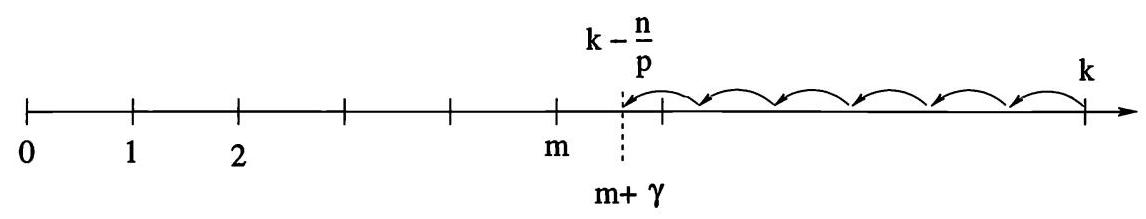
\includegraphics[width=1.0\textwidth]{images/bo_d6ik6nn7aajc739ct1l0_184_162_1681_1146_219_0.jpg}
\caption{计算函数 $f \in \; {W}^{k,p} \subset  {\mathcal{C}}^{m,\gamma }.$ 的“净光滑性”.}
\label{fig:net-smoothness}
\end{figure}

\begin{definition}{连续嵌入}
    称 Banach 空间 $X$ \colorbf{连续嵌入}于 Banach 空间 $Y$ ，若 $X \subseteq  Y$ ，且存在常数 $C$ ，使得
\[
\| u{\| }_{Y} \leq  C\| u{\| }_{X}\;\forall\,u \in  X.
\]
\end{definition}

\begin{theorem}[一般 Soblev 嵌入]\label{thm:sobolev-embedding-general}
设 $\Omega  \subset  {\mathbb{R}}^{n}$ 是具有 ${\mathcal{C}}^{1}$ 边界的有界开集，并考虑空间 ${W}^{k,p}\left( \Omega \right)$ .令 $m,\gamma$ 如\eqref{eq:net-smoothness}式所定义.则下列连续嵌入成立.
\begin{enumerate}[(i)]
    \item 若 $k - \frac{n}{p} < 0$ ，则 ${W}^{k,p}\left( \Omega \right)  \subseteq  {L}^{q}\left( \Omega \right)$ ，且 $\frac{1}{q} = \frac{1}{p} - \frac{k}{n} = \; \frac{1}{n}\left( {\frac{n}{p} - k}\right) .$
    \item 若 $k - \frac{n}{p} = 0$ ，则对每个 ${W}^{k,p}\left( \Omega \right)  \subseteq  {L}^{q}\left( \Omega \right)$ 有 $1 \leq  q < \infty$ .
    \item 若 $m \geq  0$ 且 $\gamma  > 0$ ，则 ${W}^{k,p}\left( \Omega \right)  \subseteq  {\mathcal{C}}^{m,\gamma }\left( \Omega \right)$ .
    \item 若 $m \geq  1$ 且 $\gamma  = 0$ ，则对每个 $0 \leq  {\gamma }^{\prime } < 1$ 有 ${W}^{k,p}\left( \Omega \right)  \subseteq  {\mathcal{C}}^{m - 1,{\gamma }^{\prime }}\left( \Omega \right)$ .
\end{enumerate}
\end{theorem}

\begin{remark}\label{rem:sobolev-embedding-meaning}
Soblev 空间中的函数仅在零测集意义下定义.我们说 ${W}^{k,p}\left( \Omega \right)  \subseteq  {\mathcal{C}}^{m,\gamma }\left( \Omega \right)$ ，意指如下:对每个 $u \in  {W}^{k,p}\left( \Omega \right)$ ，存在一个函数 $\widetilde{u} \in  {\mathcal{C}}^{m,\gamma }\left( \Omega \right)$ ，使得 $\widetilde{u}\left( x\right)  = \; u\left( x\right)$ 对几乎处处的 $x \in  \Omega$ 成立；此外，存在一个常数 $C$ ，它依赖于 $k,p,m,\gamma$ 但不依赖于 $u$ ，满足
\[
\| u{\| }_{{\mathcal{C}}^{m,\gamma }\left( \Omega \right) }\; \leq  \;C\| \widetilde{u}{\| }_{{W}^{k,p}\left( \Omega \right) }.
\]
\end{remark}

\begin{proof}
1．我们首先证明 (i)．假设 $k - \frac{n}{p} < 0$ ，并令 $u \in  {W}^{k,p}\left( \Omega \right)$ ．由于对每个 ${D}^{\alpha }u \in  {W}^{1,p}\left( \Omega \right)$ 有 $\left| \alpha \right|  \leq  k - 1$ ，Gagliardo-Nirenberg 不等式给出
\[
{\norm{D}^{\alpha }u}_{{L}^{{p}^{ * }}\left( \Omega \right) }\; \leq  C\norm{u}_{{W}^{k,p}\left( \Omega \right) },\;\left| \alpha \right|  \leq  k - 1\;.
\]

因此 $u \in  {W}^{k - 1,{p}^{ * }}\left( \Omega \right)$ ，其中 ${p}^{ * }$ 是 $p$ 的 Soblev 共轭指数.

该论证可迭代进行．令 ${p}_{1} = {p}^{ * },{p}_{2} \doteq  {p}_{1}^{ * },\ldots ,{p}_{j} \doteq  {p}_{j - 1}^{ * }$ ．由\eqref{eq:p-star-reciprocal}可知，当${jp} < n$时，
\[
\frac{1}{{p}_{1}} = \frac{1}{p} - \frac{1}{n},\;\ldots ,\;\frac{1}{{p}_{j}} = \frac{1}{p} - \frac{j}{n},
\]
多次应用 Gagliardo-Nirenberg 不等式，我们得到\eqref{eq:sobolev-iteration}
\begin{equation}\tag{8.70}\label{eq:sobolev-iteration}
{W}^{k,p}(\Omega )\; \subseteq  \;{W}^{k - 1,{p}_{1}}(\Omega )\; \subseteq  \;{W}^{k - 2,{p}_{2}}(\Omega )\; \subseteq  \;\cdots \; \subseteq  \;{W}^{k - j,{p}_{j}}(\Omega )\;.
\end{equation}
经过 $k$ 步后，我们得到 $u \in  {W}^{0,{p}_{k}}\left( \Omega \right)  = {L}^{{p}_{k}}\left( \Omega \right)$ ，其中 $\frac{1}{{p}_{k}} = \frac{1}{p} - \frac{k}{n} = \frac{1}{q}$ ．于是 ${p}_{k} = q$ ，(i) 得证.

\noindent 2．在特殊情形 ${kp} = n$ 下，重复上述论证，经过 $k - 1$ 步后我们得到
\[
\frac{1}{{p}_{k - 1}} = \frac{1}{p} - \frac{k - 1}{n} = \frac{1}{n}.
\]

因此 ${p}_{k - 1} = n$ ，且
\[
{W}^{k,p}\left( \Omega \right)  \subset  {W}^{1,n}\left( \Omega \right)  \subseteq  {W}^{1,n - \varepsilon }\left( \Omega \right)
\]
对每个 $\varepsilon  > 0$ 成立．再次应用 Gagliardo-Nirenberg 不等式，我们得到
\[
u \in  {W}^{1,n - \varepsilon }\left( \Omega \right)  \subseteq  {L}^{q}\left( \Omega \right) ,\;q = \frac{n\left( {n - \varepsilon }\right) }{n - \left( {n - \varepsilon }\right) } = \frac{{n}^{2} - {\varepsilon n}}{\varepsilon }.
\]

由于 $\varepsilon  > 0$ 是任意的，这就证明了 (ii).

\noindent 3．为证明 (iii)，假设 $m \geq  0$ 且 $\gamma  > 0$ ，并令 $u \in  {W}^{k,p}\left( \Omega \right)$ ．我们使用嵌入式\eqref{eq:sobolev-iteration}，选取 $j$ 为满足 ${p}_{j} > n$ 的最小整数．于是我们有
\[
\frac{1}{p} - \frac{j}{n} = \frac{1}{{p}_{j}} < \frac{1}{n} < \frac{1}{p} - \frac{j - 1}{n},\;u \in  {W}^{k - j,{p}_{j}}\left( \Omega \right) .
\]

因此，对任意满足 $\alpha$ 且 $\left| \alpha \right|  \leq  k - j - 1$ 的多重指标，Morrey 不等式给出
\[
{D}^{\alpha }u \in  {W}^{1,{p}_{j}}\left( \Omega \right)  \subseteq  {\mathcal{C}}^{0,\gamma }\left( \Omega \right) \;\text{其中}\;\gamma  = 1 - \frac{n}{{p}_{j}} = 1 - \frac{n}{p} + j.
\]

由于 $\alpha$ 是任一长度为 $\leq  k - j - 1$ 的多重指标，上述结论意味着
\[
u \in  {\mathcal{C}}^{k - j - 1,\gamma }\left( \Omega \right) \text{ . }
\]

为完成 (iii) 的证明，只需验证
\[
k - \frac{n}{p} = \left( {k - j - 1}\right)  + \left( {1 - \frac{n}{p} + j}\right) ,
\]

于是 $m = k - j - 1$ 为数 $k - \frac{n}{p}$ 的整数部分，而 $\gamma$ 为其小数部分.

\noindent 4. 为证明 (iv)，假设 $m \geq  1$ 且 $j \doteq  \frac{n}{p}$ 为整数.令 $u \in  {W}^{k,p}\left( \Omega \right)$ ，并任取满足 $\left| \alpha \right|  \leq  j - 1$ 的多重指标.仿照步骤 2 使用 Gagliardo-Nirenberg 不等式，可得
\[
{D}^{\alpha }u \in  {W}^{k - j,p}\left( \Omega \right)  \subseteq  {W}^{1,q}\left( \Omega \right)
\]
对每个 $1 < q < \infty$ 成立.故由 Morrey 不等式
\[
{D}^{\alpha }u \in  {W}^{1,q}\left( \Omega \right)  \subseteq  {\mathcal{C}}^{0,1 - \frac{n}{q}}\left( \Omega \right) .
\]

由于 $q$ 可任意大，这便证明了 (iv).
\end{proof}

\begin{instance}\label{ins:sobolev-embedding-example}
设 $\Omega$ 为 ${\mathbb{R}}^{5}$ 中的开单位球，并设 $u \in  {W}^{4,2}\left( \Omega \right)$ .连续两次应用 Gagliardo-Nirenberg 不等式，再应用 Morrey 不等式，可得
\[
u \in  {W}^{4,2}\left( \Omega \right)  \subset  {W}^{3,\frac{10}{3}}\left( \Omega \right)  \subset  {W}^{2,{10}}\left( \Omega \right)  \subset  {C}^{1,\frac{1}{2}}\left( \Omega \right) .
\]

注意， $u$ 的净光滑性为 $k - \frac{n}{p} = 4 - \frac{5}{2} = 1 + \frac{1}{2}.$
\end{instance}

\section{紧嵌入}

设 $\Omega  \subset  {\mathbb{R}}^{n}$ 为具有 ${\mathcal{C}}^{1}$ 边界的有界开集.本节将更深入地研究嵌入 ${W}^{1,p}\left( \Omega \right)  \subset  {L}^{q}\left( \Omega \right)$ ，并证明:当 $\frac{1}{q} > \frac{1}{p} - \frac{1}{n}$ 时，该嵌入是紧的.即，对任意在 ${W}^{1,p}$ 中有界的序列 ${\left( {u}_{m}\right) }_{m \geq  1}$ ，均可提取一个在 ${L}^{q}$ 中收敛的子列.

作为预备，我们注意到:若 $p > n$ ，则每个函数 $u \in \; {W}^{1,p}\left( \Omega \right)$ 均为 Hölder 连续.特别地，若 ${\left( {u}_{m}\right) }_{m \geq  1}$ 是 ${W}^{1,p}\left( \Omega \right)$ 中的有界序列，则函数族 ${u}_{m}$ 等度连续且一致有界.由 Arzelà-Ascoli 紧性定理，可提取子列 ${\left( {u}_{{m}_{j}}\right) }_{j \geq  1}$ ，其在 $\Omega$ 上一致收敛于某个连续函数 $u$ .由于 $\Omega$ 有界，这蕴含对每个 $q \in  \left(  {1,\infty }\right)$ 均有 ${\norm{u}_{{m}_{j}} - u}_{{L}^{q}\left( \Omega \right) } \rightarrow  0$ .这已表明:当 $p > n$ 且 $1 \leq  q \leq  \infty$ 时，嵌入 ${W}^{1,p}\left( \Omega \right)  \subset  {L}^{q}\left( \Omega \right)$ 是紧的.

因此，本节余下部分我们聚焦于情形 $p < n$ .由Gagliardo-Nirenberg不等式，空间 ${W}^{1,p}\left( \Omega \right)$ 连续嵌入于 ${L}^{{p}^{ * }}\left( \Omega \right)$ ，其中 ${p}^{ * } = \frac{np}{n - p}$ .进而，由于 $\Omega$ 有界，对每个 $1 \leq  q \leq  {p}^{ * }$ ，我们有连续嵌入 ${L}^{{p}^{ * }}\left( \Omega \right)  \subseteq  {L}^{q}\left( \Omega \right)$ .

\begin{theorem}[Rellich--Kondrachov紧性定理]\label{thm:rellich-kondrachov}
设 $\Omega  \subset  {\mathbb{R}}^{n}$ 为具有 ${\mathcal{C}}^{1}$ 边界的有界开集，且假设 $1 \leq  p < n$ .则对每个 $1 \leq  q < {p}^{ * } \doteq  \frac{np}{n - p}$ ，均有紧嵌入
\begin{equation}\tag{8.71}\label{eq:rellich-kondrachov}
{W}^{1,p}\left( \Omega \right)  \subset  \subset  {L}^{q}\left( \Omega \right) .
\end{equation}
\end{theorem}

\begin{proof}
1. 设 ${\left( {u}_{m}\right) }_{m \geq  1}$ 为 ${W}^{1,p}\left( \Omega \right)$ 中的有界序列.利用Soblev函数延拓定理\ref{thm:extension-operator}，可假设所有函数 ${u}_{m}$ 均定义在整个空间 ${\mathbb{R}}^{n}$ 上，且在某个紧集 $K$ 外恒为零:
\begin{equation}\tag{8.72}\label{eq:rellich-support}
\operatorname{Supp}\left( {u}_{m}\right)  \subseteq  K \subset  \widetilde{\Omega } \doteq  B\left( {\Omega ,1}\right) .
\end{equation}

此处右端表示围绕集合 $\Omega$ 的半径为一的开邻域.

由于 $q < {p}^{ * }$ 与 $\widetilde{\Omega }$ 有界，我们有
\[
{\norm{u}_{m}}_{{L}^{q}\left( {\mathbb{R}}^{n}\right) }  =  {\norm{u}_{m}}_{{L}^{q}\left( \widetilde{\Omega }\right) }  \leq   C {\norm{u}_{m}}_{{L}^{{p}^{ * }}\left( \widetilde{\Omega }\right) }  \leq   {C}^{\prime } {\norm{u}_{m}}_{{W}^{1,p}\left( \widetilde{\Omega }\right) }
\]

对某些常数 $C,{C}^{\prime }$ 成立.故序列 ${u}_{m}$ 在 ${L}^{q}\left( {\mathbb{R}}^{n}\right)$ 中一致有界.

\noindent 2. 考虑磨光函数 ${u}_{m}^{\varepsilon } \doteq  {J}_{\varepsilon } * {u}_{m}$ .由\eqref{eq:rellich-support}可知，所有这些函数均支撑于 $\widetilde{\Omega }$ 内.我们声称\eqref{eq:rellich-mollifier-conv}
\begin{equation}\tag{8.73}\label{eq:rellich-mollifier-conv}
{\norm{u_{m}^{\varepsilon } - {u}_{m}}}_{{L}^{q}\left( \widetilde{\Omega }\right) } \rightarrow  0,\;\;\varepsilon  \rightarrow  0,\;\text{关于}\;m\;\text{一致}.
\end{equation}

事实上，若 ${u}_{m}$ 光滑，则(作变量替换 ${y}^{\prime } = {\varepsilon y}$ 与 $z = x - {\varepsilon ty})$
{\setjot[-1]\begin{align*}
{u}_{m}^{\varepsilon }\left( x\right)  - {u}_{m}\left( x\right)  &= {\int }_{\left| {y}^{\prime }\right|  < \varepsilon }{J}_{\varepsilon }\left( {y}^{\prime }\right) \left(  {{u}_{m}\left( {x - {y}^{\prime }}\right)  - {u}_{m}\left( x\right) }\right)  d{y}^{\prime }\\
&= {\int }_{\left| y\right|  < 1}J\left( y\right) \left(  {{u}_{m}\left( {x - {\varepsilon y}}\right)  - {u}_{m}\left( x\right) }\right)  {\d y}\\
&= {\int }_{\left| y\right|  < 1}J\left( y\right) \left( {{\int }_{0}^{1}\frac{d}{\d t}\left( {{u}_{m}\left( {x - {\varepsilon ty}}\right) }\right) {\d t}}\right) {\d y}\\
&=  - \varepsilon {\int }_{\left| y\right|  < 1}J\left( y\right) \left( {{\int }_{0}^{1}\nabla {u}_{m}\left( {x - {\varepsilon ty}}\right)  \cdot  {y\d t}}\right) {\d y}.
\end{align*}}

进而得到
\begin{align*}
    \int_{\widetilde{\Omega }}\left| {u_m^{\varepsilon }(x)-u_m(x) }\right| {\d x} &\leq  \varepsilon {\int }_{\widetilde{\Omega }}{\int }_{\left| y\right| \leq  1}J\left( y\right) \left( {{\int }_{0}^{1}\left| {\nabla {u}_{m}\left( {x - {\varepsilon ty}}\right) }\right| {\d t}}\right) {\d y\d x}\\
    &\leq  \varepsilon {\int }_{\widetilde{\Omega }}\left| {\nabla {u}_{m}\left( z\right) }\right| {\d z}
\end{align*}


通过在 ${W}^{1,p}$ 中用光滑函数列逼近 ${u}_{m}$ ，可知该估计对所有函数 ${u}_{m} \in  {W}^{1,p}\left( \widetilde{\Omega }\right)$ 仍成立.因此我们已证得
\begin{equation}\tag{8.74}\label{eq:rellich-L1-estimate}
\norm{{u}_{m}^{\varepsilon }-{u}_{m}}_{{L}^{1}\left( \widetilde{\Omega }\right) }  \leq   \varepsilon \norm{\nabla {u}_{m}}_{{L}^{1}\left( \widetilde{\Omega }\right) }  \leq   {\varepsilon C}{\norm{u}_{m}}_{{W}^{1,p}\left( \widetilde{\Omega }\right) },
\end{equation}
对某个与 $m$ 无关的常数 $C$ 成立.由于范数 ${\norm{u}_{m}}_{{W}^{1,p}}$ 关于 $m$ 具有一致上界，这已证得我们在 $q = 1$ 情形下的断言\eqref{eq:rellich-mollifier-conv}.

\noindent 3. 为证 $1 < q < {p}^{ * }$ 情形下的\eqref{eq:rellich-mollifier-conv}，现使用 ${L}^{p}$ 范数的插值不等式(见附录(A.28)).选取 $0 < \theta  < 1$ 使得
\[
\frac{1}{q} = \theta  \cdot  1 + \left( {1 - \theta }\right)  \cdot  \frac{1}{{p}^{ * }}.
\]

则
\begin{equation}\tag{8.75}\label{eq:rellich-interpolation}
\| {u}_{m}^{\varepsilon } - {u}_{m} \|_{{L}^{q}\left( \widetilde{\Omega }\right) } \leq  \| {u}_{m}^{\varepsilon } - {u}_{m} \|_{{L}^{1}\left( \widetilde{\Omega }\right) }^{\theta } \cdot  \| {u}_{m}^{\varepsilon } - {u}_{m} \|_{{L}^{{p}^{ * }}\left( \widetilde{\Omega }\right) }^{1 - \theta } \leq  \left( {C}_{0}\varepsilon \right) ^{\theta }.
\end{equation}
对某个与 $m$ 无关的常数 ${C}_{0}$ 成立.事实上，在上述表达式中， ${L}^{1}$ 范数由\eqref{eq:rellich-L1-estimate}控制，而 ${L}^{{p}^{ * }}$ 范数则由定理\ref{thm:gagliardo-nirenberg}控制为某常数.

\noindent 4. 任取 $\delta  > 0$ ，并选取足够小的 $\varepsilon  > 0$ ，使得\eqref{eq:rellich-interpolation}给出
\[
{\norm{u}_{m}^{\varepsilon } - {u}_{m}}_{{L}^{q}\left( \widetilde{\Omega }\right) } \leq  {C}_{0}{\varepsilon }^{\theta } \leq  \frac{\delta }{2}\;\forall\,m \geq  1.
\]

回顾 ${u}_{m}^{\varepsilon } = {J}_{\varepsilon } * {u}_{m}$ ，我们有
{\begin{gather*}
    {\norm{u}_{m}^{\varepsilon }}_{{L}^{\infty }} \leq  {\norm{J}_{\varepsilon }}_{{L}^{\infty }}{\norm{u}_{m}}_{{L}^{1}} \leq  {C}_{1}\\
    \norm{\nabla {u}_{m}^{\varepsilon }}_{{L}^{\infty }} \leq  \norm{\nabla {J}_{\varepsilon }}_{{L}^{\infty }}{\norm{u}_{m}}_{{L}^{1}} \leq  {C}_{2}
\end{gather*}}
其中 ${C}_{1},{C}_{2}$ 是仅依赖于 $\varepsilon$ 而与 $m$ 无关的常数.上述不等式表明，对每个固定的 $\varepsilon  > 0$，序列 ${\left( {u}_{m}^{\varepsilon }\right) }_{m \geq  1}$ 一致有界且等度连续.由Ascoli紧性定理，存在子列 $\left( {u}_{{m}_{j}}^{\varepsilon }\right)$ 在 $\widetilde{\Omega }$ 上一致收敛于某个连续函数 ${u}^{\varepsilon }$ .我们现得到
\begin{equation}\tag{8.76}\label{eq:rellich-cauchy-estimate}
\begin{aligned}
\limsup_{{j,k \rightarrow  \infty }}\norm{{u}_{{m}_{j}} - {u}_{{m}_{k}}}_{{L}^{q}}
&\leq  \limsup_{{j,k \rightarrow  \infty }}\Bigl(
\norm{{u}_{{m}_{j}} - {u}_{{m}_{j}}^{\varepsilon }}_{{L}^{q}}
+ \norm{{u}_{{m}_{j}}^{\varepsilon } - {u}^{\varepsilon }}_{{L}^{q}} \\
&\quad +\norm{{u}^{\varepsilon } - {u}_{{m}_{k}}^{\varepsilon }}_{{L}^{q}}+\norm{{u}_{{m}_{k}}^{\varepsilon } - {u}_{{m}_{k}}}_{{L}^{q}}\Bigr) \\
&\leq  \frac{\delta }{2} + 0 + 0 + \frac{\delta }{2}.
\end{aligned}
\end{equation}

\noindent 5. 证明现通过标准对角化论证完成.由前一步可知，存在一个无穷指标集 ${I}_{1} \subset  \mathbb{N}$ ，使得子列 ${\left( {u}_{m}\right) }_{m \in  {I}_{1}}$ 满足
\[
\limsup_{{\ell ,m \rightarrow  \infty ,\ell ,m \in  {I}_{1}}}{\norm{u}_{\ell } - {u}_{m}}_{{L}^{q}} \leq  {2}^{-1}
\]

对 $j = 1,2,\ldots$ 归纳:在 ${I}_{j - 1}$ 构造完成后，选取一个无穷指标集 ${I}_{j} \subset  {I}_{j - 1} \subset  \mathbb{N}$ ，使得子列 ${\left( {u}_{m}\right) }_{m \in  {I}_{j}}$ 满足
\[
\limsup_{{\ell ,m \rightarrow  \infty ,\ell ,m \in  {I}_{j}}}{\norm{u}_{\ell } - {u}_{m}}_{{L}^{q}} \leq  {2}^{-j}
\]

在对所有 $j \geq  1$ 构造完子集 ${I}_{j}$ 后，再对 $j$ 归纳，选取一列整数 ${m}_{1} < {m}_{2} < {m}_{3} < \cdots$ ，使得对每个 $j$ 均有 ${m}_{j} \in  {I}_{j}$ .该子列 ${\left( {u}_{{m}_{j}}\right) }_{j \geq  1}$ 满足
\[
\limsup_{{j,k \rightarrow  \infty }}{\norm{u}_{{m}_{j}} - {u}_{{m}_{k}}}_{{L}^{q}} = 0.
\]

因此该子列是Cauchy列，收敛于某个极限 $u \in  {L}^{q}$ .这证明了当 $p < n$ 时嵌入\eqref{eq:rellich-kondrachov}是紧的.
\end{proof}

\begin{corollary}\label{cor:H1-L2-compact-embedding}
设 $\Omega  \subset  {\mathbb{R}}^{n}$ 是具有 ${\mathcal{C}}^{1}$ 边界的有界开集，则有如下紧嵌入
\[
{H}^{1}\left( \Omega \right)  \subset  \subset  {L}^{2}\left( \Omega \right) .
\]
\end{corollary}

\begin{proof}
当 $n > 2$ 时，结论是定理\ref{thm:rellich-kondrachov}(取 $p = 2$ )的特例；当 $n = 1$ 时， ${H}^{1}\left( \Omega \right)$ 中每个函数均为Hölder连续，结果由 Ascoli 定理得出；当 $n = 2$ 时，可对 $p = 3/2,{p}^{ * } = 6,q = 2$ 应用定理\ref{thm:rellich-kondrachov}，得到
\[
{W}^{1,2}\left( \Omega \right)  \subset  {W}^{1,3/2}\left( \Omega \right)  \subset  \subset  {L}^{2}\left( \Omega \right) .
\]
\end{proof}

作为紧嵌入定理的一个应用，我们现证明函数 $u$ 与其在区域 $\Omega$ 上平均值之差的一个估计.

\begin{theorem}[Poincar\'e不等式 II]\label{thm:poincare-inequality-ii}
设 $\Omega  \subset  {\mathbb{R}}^{n}$ 是具有 ${\mathcal{C}}^{1}$ 边界的有界连通开集，且设 $p \in  \left(  {1,\infty }\right)$ .则存在仅依赖于 $p$ 和 $\Omega$ 的常数 $C$ ，使得
\begin{equation}\tag{8.77}\label{eq:poincare-ii}
\norm{u - {\int }_{\Omega }u\,\d x}_{{L}^{p}\left( \Omega \right) }\; \leq  \;C\norm{\nabla u}_{{L}^{p}\left( \Omega \right) }.
\end{equation}

对每个 $u \in  {W}^{1,p}\left( \Omega \right)$ 成立.
\end{theorem}

\begin{proof}
若结论不成立，则可找到一列函数 ${u}_{k} \in  {W}^{1,p}\left( \Omega \right)$ ，满足
\[
\norm{{u}_{k} - {\int }_{\Omega }{u}_{k}\,\d x}_{{L}^{p}\left( \Omega \right) } > k\norm{\nabla {u}_{k}}_{{L}^{p}\left( \Omega \right) }
\]

对每个 $k = 1,2,\ldots$ 成立.于是归一化函数
\[
{v}_{k} \doteq  \frac{{u}_{k} - {\int }_{\Omega }{u}_{k}\,\d x}{\norm{{u}_{k} - {\int }_{\Omega }{u}_{k}\,\d x}_{{L}^{p}\left( \Omega \right) }}
\]
满足
\begin{equation}\tag{8.78}\label{eq:poincare-ii-normalization}
{\int }_{\Omega }{v}_{k}\,\d x = 0,\;{\norm{v}_{k}}_{{L}^{p}\left( \Omega \right) } = 1,\;{\norm{\nabla {v}_{k}}}_{{L}^{p}\left( \Omega \right) } < \frac{1}{k},\;k = 1,2,\ldots
\end{equation}

由于序列 ${\left( {v}_{k}\right) }_{k \geq  1}$ 在 ${W}^{1,p}\left( \Omega \right)$ 中有界，若 $p < n$ ，则可应用定理\ref{thm:rellich-kondrachov}(取 $q = p$ )，找到一个在 ${L}^{p}\left( \Omega \right)$ 中收敛于某个函数 $v$ 的子列.若 $p > n$ ，则由\eqref{eq:morrey-embedding}可知函数 ${v}_{k}$ 一致有界且 Hölder 连续.于是利用 Ascoli 紧性定理，可找到一个在 $\Omega$ 上一致收敛于某个连续函数 $v$ 的子列，从而也在 ${L}^{p}\left( \Omega \right)$ 中收敛于 $v$.

由\eqref{eq:poincare-ii-normalization}，弱梯度序列亦收敛，即 $\nabla {v}_{k} \to 0$ 于 ${L}^{p}\left( \Omega \right)$ 中.由引理 8.14，零函数是极限函数 $v$ 的弱梯度.

我们现已有
\[
{\int }_{\Omega }v\,\d x = \mathop{\lim }\limits_{{k \rightarrow  \infty }}{\int }_{\Omega }{v}_{k}\,\d x = 0.
\]
此外，由于 $\nabla v = 0 \in  {L}^{p}\left( \Omega \right)$ ，由推论 8.16 可知函数 $v$ 在连通集 $\Omega$ 上必为常数；结合 $\int_{\Omega } v\,\d x = 0$ ，可得 $v = 0$ 几乎处处成立.

另一方面，由 ${v}_{k} \to v$ 于 ${L}^{p}\left( \Omega \right)$ 及\eqref{eq:poincare-ii-normalization}可得 $\norm{v}_{{L}^{p}\left( \Omega \right) } = 1$ ，矛盾.
\end{proof}

\section{可微性性质}

由 Morrey 不等式，若 $\Omega  \subset  {\mathbb{R}}^{n}$ 且 $w \in  {W}^{1,p}\left( \Omega \right)$ 满足 $p > n$ ，则 $w$ 几乎处处等于一个 Hölder 连续函数.事实上，在零测集上适当修改后，我们有
\begin{equation}\tag{8.79}\label{eq:morrey-pointwise}
\left| {w\left( x\right)  - w\left( y\right) }\right|  \leq  C{\left| x - y\right| }^{1 - \frac{n}{p}}{\left( {\int }_{B\left( {x,\left| {y - x}\right| }\right) }{\left| \nabla w\left( z\right) \right| }^{p}\d z\right) }^{1/p}.
\end{equation}

仅此本身并不意味着 $u$ 必须在经典意义下可微.事实上，存在处处不可微的 Hölder 连续函数.然而，对 Soblev 空间中的函数，可证明更强的正则性结果.

\begin{theorem}[几乎处处可微性]\label{thm:a-e-differentiability}
设 $\Omega  \subseteq  {\mathbb{R}}^{n}$ ，且对某个 $p > n$ 有 $u \in  {W}_{\text{ loc }}^{1,p}\left( \Omega \right)$ .则 $u$ 在几乎处处的点 $x \in  \Omega$ 可微，且其梯度与弱梯度重合.
\end{theorem}

\begin{proof}
令 $u \in  {W}_{\text{ loc }}^{1,p}\left( \Omega \right)$ .由于弱导数属于 ${L}_{\text{ loc }}^{p}$ ，弱梯度 $\nabla u \doteq  \left( {{D}_{{x}_{1}}u,\ldots ,{D}_{{x}_{n}}u}\right)$ 同样属于 ${L}_{\text{ loc }}^{p}$ .由 Lebesgue 微分定理，对几乎处处的 $x \in  \Omega$ ，有
\begin{equation}\tag{8.80}\label{eq:lebesgue-diff-grad}
{\oint }_{B\left( {x,r}\right) }{\left| \nabla u\left( x\right)  - \nabla u\left( z\right) \right| }^{p}{\d z} \rightarrow  0\;\text{ as }r \rightarrow  0.
\end{equation}

固定一个满足\eqref{eq:lebesgue-diff-grad}的点 $x$ ，并定义
\begin{equation}\tag{8.81}\label{eq:def-w-for-diff}
w\left( y\right)  \doteq  u\left( y\right)  - u\left( x\right)  - \nabla u\left( x\right)  \cdot  \left( {y - x}\right) .
\end{equation}

注意到 $w \in  {W}_{\text{ loc }}^{1,p}\left( \Omega \right)$ ，可应用估计式\eqref{eq:morrey-pointwise}，得

{\begin{align*}
    \left| {w\left( y\right)  - w\left( x\right) }\right|  &= \left| {w\left( y\right) }\right|  = \left| {u\left( y\right)  - u\left( x\right)  - \nabla u\left( x\right)  \cdot  \left( {y - x}\right) }\right|\\
    &\leq  C{\left| y - x\right| }^{1 - \frac{n}{p}}{\left( {\int }_{B\left( {x,\left| {y - x}\right| }\right) }{\left| \nabla u\left( x\right)  - \nabla u\left( z\right) \right| }^{p}\d z\right) }^{1/p}\\
    &\leq  {C}^{\prime }\left| {y - x}\right| {\left( {f}_{B\left( {x,\left| {y - x}\right| }\right) }{\left| \nabla u\left( x\right)  - \nabla u\left( z\right) \right| }^{p}\d z\right) }^{1/p}
\end{align*}}
对某些常数 $C,{C}^{\prime }$ 成立.因此
\[
\frac{\left| w\left( y\right)  - w\left( x\right) \right| }{\left| y - x\right| } \rightarrow  0\;\text{ as }\left| {y - x}\right|  \rightarrow  0.
\]

由\eqref{eq:def-w-for-diff}中 $w$ 的定义可知， $u$ 在 $x$ 处经典可微，且其梯度与弱梯度重合.
\end{proof}

\section{习题}

\begin{rbhw}[index=1]
判定下列泛函中哪些在 $\Omega  \subseteq  \mathbb{R}$ 上定义了一个分布.
\begin{enumerate}[(i)]
    \item $\Lambda \left( \phi \right)  = \sum_{{k = 1}}^{\infty }k!{D}^{k}\phi \left( k\right)$ ，其中 $\Omega  = \mathbb{R}$ .
    \item $\Lambda \left( \phi \right)  = \sum_{{k = 1}}^{\infty }{2}^{-k}{D}^{k}\phi \left( {1/k}\right)$ ，且 $\Omega  = \mathbb{R}$ .
    \item $\Lambda \left( \phi \right)  = \sum_{{k = 1}}^{\infty }\frac{\phi \left( {1/k}\right) }{k}$ ，且 $\Omega  = \mathbb{R}$ .
    \item $\Lambda \left( \phi \right)  = {\int }_{0}^{\infty }\frac{\phi \left( x\right) }{{x}^{2}}\,\d x$ ，且 $\Omega = (0,\infty)$ .
\end{enumerate}
\end{rbhw}

\begin{rbhw}
给出直接证明:若对某个 $f \in  {W}^{1,p}(a,b)$ 、 $a < b$ 和 $1 < p < \infty$ ，则通过在零测集上修改 $f$ ，可得
\[
\left| {f\left( x\right)  - f\left( y\right) }\right|  \leq  C{\left| x - y\right| }^{1 - \frac{1}{p}}\;\forall\,x,y \in  ( a,b) .
\]
计算最优常数 $C$ .
\end{rbhw}

\begin{rbhw}
考虑开正方形
\[
Q \doteq  \left\{  {\left( {{x}_{1},{x}_{2}}\right) ;0 < {x}_{1} < 1,0 < {x}_{2} < 1}\right\}   \subset  {\mathbb{R}}^{2}.
\]

设 $f \in  {W}^{1,1}\left( Q\right)$ 为一函数，其弱导数满足对几乎处处 $x \in  Q$ 有 ${D}_{{x}_{1}}f\left( x\right)  = 0$ .证明存在一函数 $g \in  {L}^{1}\left( \left(  {0,1}\right)  \right)$ ，使得
\[
f\left( {{x}_{1},{x}_{2}}\right)  = g\left( {x}_{2}\right) \;\text{ for a.e. }\left( {{x}_{1},{x}_{2}}\right)  \in  Q.
\]
\end{rbhw}

\begin{rbhw}
设 $\Omega  \subseteq  {\mathbb{R}}^{n}$ 为开集，且假设 $f \in  {L}_{\text{ loc }}^{1}\left( \Omega \right)$ .设 $g = {D}_{{x}_{1}}f$ 为 $f$ 关于 ${x}_{1}$ 的弱导数.若 $f$ 在开子集 ${\Omega }^{\prime } \subseteq  \Omega$ 上等于 ${\mathcal{C}}^{1}$ ，则证明 $g$ 在几乎处处点 $x \in  {\Omega }^{\prime }$ 上与偏导数 $\partial f/\partial {x}_{1}$ 重合.
\end{rbhw}

\begin{rbhw}
(i) 证明:若对某个开凸集 $\Omega  \subseteq  {\mathbb{R}}^{n}$ 有 $u \in  {W}^{1,\infty }\left( \Omega \right)$ ，则 $u$ 几乎处处与一个Lipschitz连续函数重合.

(ii) 证明:存在一个(非凸的)连通开集 $\Omega  \subset  {\mathbb{R}}^{n}$ 及一个函数 $u \in  {W}^{1,\infty }\left( \Omega \right)$ ，其不与任何Lipschitz连续函数几乎处处重合.
\end{rbhw}

\begin{rbhw}
(Rademacher定理)设 $\Omega  \subset  {\mathbb{R}}^{n}$ 为开集， $u : \Omega  \mapsto  \mathbb{R}$ 为有界Lipschitz连续函数.
\begin{enumerate}[(i)]
    \item 证明: $u \in  {W}^{1,\infty }\left( \Omega \right)$ .
    \item 证明: $u$ 在几乎处处点 $x \in  \Omega$ 上可微.
\end{enumerate}
\textcolor{gray}{(i) 的提示:先考虑 $\Omega$ 为凸集的情形.为构造弱导数 ${D}_{{x}_{i}}$ ，对任意固定 ${x}_{1},\ldots ,{x}_{i - 1},{x}_{i + 1},\allowbreak \ldots ,{x}_{n}$，考虑绝对连续函数 $s \mapsto  u( {x}_{1},\ldots ,{x}_{i - 1},s,{x}_{i + 1},\ldots ,{x}_{n} )$ .}
\end{rbhw}

\begin{rbhw}
设 $\Omega  = B\left( {0,1}\right)$ 为 ${\mathbb{R}}^{n}$ 中的开单位球，其中 $n \geq  2$ .证明无界函数 $f\left( x\right)  = \ln \ln \left( {1 + \frac{1}{\left| x\right| }}\right)$ 属于 ${W}^{1,n}\left( \Omega \right)$ .
\end{rbhw}

\begin{rbhw}
(i) 设 $\Omega  = (-1,1)$ .考虑由 ${Tf} = f\left( 0\right)$ 定义的线性映射 $T : {\mathcal{C}}^{1}\left( \Omega \right)  \mapsto  \mathbb{R}$ .证明该映射可唯一连续延拓为一个有界线性泛函 $T : {W}^{1,1}\left( \Omega \right)  \mapsto  \mathbb{R}$ .\par
\indent (ii) 设 $\Omega  = B\left( {0,1}\right)  \subset  {\mathbb{R}}^{2}$ 为开单位圆盘.再次考虑由 ${Tf} = f\left( 0\right)$ 定义的线性映射 $T : {\mathcal{C}}^{1}\left( \Omega \right)  \mapsto  \mathbb{R}$ .对该映射，当 $p$ 取何值时，它可连续延拓为一个有界线性泛函 $T : {W}^{1,p}\left( \Omega \right)  \mapsto  \mathbb{R}$ ？
\end{rbhw}

\begin{rbhw}
确定对哪些 $p \geq  1$ 值，一般函数 $f \in  {W}^{1,p}\left( {\mathbb{R}}^{3}\right)$ 沿 ${x}_{1}$ -轴存在迹.换言之，令 $\Gamma  \doteq  \{ \left( {t,0,0}\right) ;t \in  \mathbb{R}\}  \subset  {\mathbb{R}}^{3}$ ，并考虑映射 $T : {\mathcal{C}}_{\mathrm{c}}^{1}\left( {\mathbb{R}}^{3}\right)  \mapsto  {L}^{p}\left( \Gamma \right)$ ，其中 ${Tf} = {f}_{\mid \Gamma }$ 是 $f$ 在 $\Gamma$ 上的限制.求使该映射存在连续延拓 $T : {W}^{1,p}\left( {\mathbb{R}}^{3}\right)  \mapsto  {L}^{p}\left( \Gamma \right)$ 的 $p$ 值.
\end{rbhw}

\begin{rbhw}
设 $V \subset  {\mathbb{R}}^{n}$ 是维数为 $m$ 的子空间， ${V}^{ \bot  }$ 是其正交补子空间，维数为 $n - m$ .设 $u \in  {W}^{1,p}\left( {\mathbb{R}}^{n}\right)$ 且 $m < p < n$ .证明:在零测集上适当修改后，以下结论成立.
\begin{enumerate}[(i)]
    \item 对几乎处处的 $y \in  {V}^{ \bot  }$ (关于 $\left( {n - m}\right)$ -维测度)， $u$ 在仿射子空间 $y + V$ 上的限制是指数为 $\gamma  = 1 - \frac{m}{p}$ 的 Hölder 连续函数.
    \item 点态值 $u\left( y\right)$ 对几乎处处的 $y \in  {V}^{ \bot  }$ 有定义.此外
\[
\| u\left( y\right) {\| }_{{L}^{p}\left( {V}^{ \bot  }\right) } \leq  C \cdot  \| u{\| }_{{W}^{1,p}\left( {\mathbb{R}}^{n}\right) }
\]
其中常数 $C$ 依赖于 $m,n,p$ ，但与 $u$ 无关.
\end{enumerate}
\end{rbhw}

\begin{rbhw}
设 $\Omega  \subset  {\mathbb{R}}^{n}$ 为任意开集(不假设边界具有任何正则性)，并设 $p > n$ .证明:每个函数 $f \in  {W}_{0}^{1,p}\left( \Omega \right)$ 几乎处处等于某个连续函数 $\widetilde{f}$ .此外，存在一个常数 $C$ ，其仅依赖于 $p,n$ ，而与 $\Omega$ 或 $f$ 无关，使得
\[
\| \widetilde{f}{\| }_{{\mathcal{C}}^{0,\gamma }\left( \Omega \right) } \leq  C\| f{\| }_{{W}^{1,p}\left( \Omega \right) }\;\text{ with }\gamma  = 1 - \frac{n}{p}.
\]
\end{rbhw}

\begin{rbhw}
当 $k = 0$ 时，依定义有 ${W}^{0,p}\left( \Omega \right)  = {L}^{p}\left( \Omega \right)$ .若 $1 \leq  p < \infty$ ，则证明 ${W}_{0}^{0,p}\left( \Omega \right)  = {L}^{p}\left( \Omega \right)$ 亦成立. ${W}_{0}^{0,\infty }\left( \Omega \right)$ 是什么？
\end{rbhw}

\begin{rbhw}
设 $\varphi  : \mathbb{R} \mapsto  \left(  {0,1}\right)$ 为一光滑函数，满足
\[
\varphi \left( r\right)  =\begin{cases} 1 & \text{ if }r \leq  0, \\  0 & \text{ if }r \geq  1. \end{cases}
\]
对任意 $f \in  {W}^{k,p}\left( {\mathbb{R}}^{n}\right)$ ，证明函数 ${f}_{k}\left( x\right)  = f\left( x\right) \varphi \left( {\left| x\right|  - k}\right)$ 在 ${W}^{k,p}\left( {\mathbb{R}}^{n}\right)$ 中收敛于 $f$，对每个 $k \geq  0$ 和 $1 \leq  p < \infty$ 均成立.由此推出， ${W}_{0}^{k,p}\left( {\mathbb{R}}^{n}\right)  = {W}^{k,p}\left( {\mathbb{R}}^{n}\right) .$
\end{rbhw}

\begin{rbhw}
设 ${\mathbb{R}}_{ + } \doteq  \{ x \in  \mathbb{R};x > 0\}$ ，并假设 $u \in  {W}^{2,p}\left( {\mathbb{R}}_{ + }\right)$ .通过定义 $u$ 的对称延拓: ${Eu}\left( x\right)  \doteq  u\left( \left| x\right| \right)$ .证明 ${Eu} \in  {W}^{1,p}\left( \mathbb{R}\right)$ ，但一般地 ${Eu} \notin \; {W}^{2,p}\left( \mathbb{R}\right)$ .
\end{rbhw}

\begin{rbhw}
设 $u \in  {\mathcal{C}}_{c}^{1}\left( {\mathbb{R}}^{n}\right)$ ，并固定 $p,q \in  (1,\infty)$ .对给定的 $\lambda  > 0$ ，考虑其缩放函数 ${u}_{\lambda }\left( x\right)  \doteq  u\left( {\lambda x}\right)$ .
\begin{enumerate}[(i)]
    \item 证明存在一个依赖于 $n,q$ 的指数 $\alpha$ ，使得
\[
{\norm{u}_{\lambda }}_{{L}^{q}\left( {\mathbb{R}}^{n}\right) } = {\lambda }^{\alpha }\| u{\| }_{{L}^{q}\left( {\mathbb{R}}^{n}\right) }.
\]
    \item 证明存在一个依赖于 $n,p$ 的指数 $\beta$ ，使得
\[
\| \nabla {u}_{\lambda }{\| }_{{L}^{p}\left( {\mathbb{R}}^{n}\right) } = {\lambda }^{\beta }\| \nabla u{\| }_{{L}^{p}\left( {\mathbb{R}}^{n}\right) }.
\]
    \item  确定使 $\alpha  = \beta$ 成立的 $n,p,q$ 的取值范围，并与\eqref{eq:p-star}比较.
\end{enumerate}
\end{rbhw}

\begin{rbhw}
设 $\Omega  \subset  {\mathbb{R}}^{n}$ 是具有 ${\mathcal{C}}^{1}$ 边界的有界开集， ${\left( {u}_{m}\right) }_{m \geq  1}$ 是一列在 ${H}^{1}\left( \Omega \right)$ 中一致有界的函数.若假设 ${\norm{u}_{m} - u}_{{L}^{2}} \rightarrow  0$ ，则证明 $u \in  {H}^{1}\left( \Omega \right)$ ，且
\[
\| u{\| }_{{H}^{1}} \leq  \mathop{\liminf }\limits_{{m \rightarrow  \infty }}{\norm{u}_{m}}_{{H}^{1}}.
\]
\end{rbhw}

\begin{rbhw}
设 $\Omega  \doteq  \left\{  {\left( {{x}_{1},{x}_{2}}\right) ;{x}_{1}^{2} + {x}_{2}^{2} < 1}\right\}$ 为 ${\mathbb{R}}^{2}$ 中的开单位圆盘， ${\Omega }_{0} \doteq  \Omega  \setminus  \{ \left( {0,0}\right) \}$ 为去掉原点的单位圆盘.考虑函数 $f\left( x\right)  \doteq  1 - \left| x\right|$ .证明(见图\ref{fig:exercise-17})
\begin{enumerate}[(i)]
    \item  若$1 \leq  p < \infty$，则$f  \in  {W}_{0}^{1,p}\left( \Omega \right)$.
    \item 若$1 \leq  p \leq  2$，则$f  \in  {W}_{0}^{1,p}\left( {\Omega }_{0}\right)$；
    \item 若$2 < p \leq  \infty$，则$f  \notin  {W}_{0}^{1,p}\left( \Omega \right)$.
\end{enumerate}
\begin{figure}[htbp]
\centering
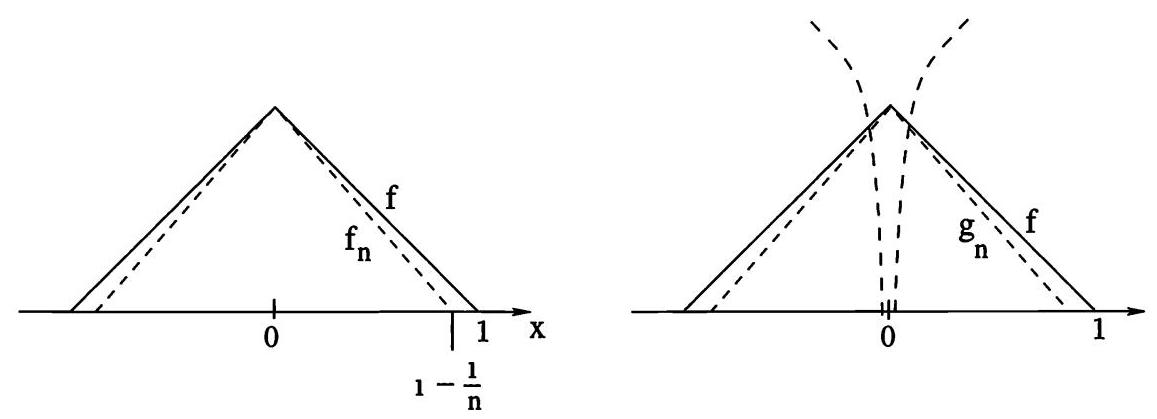
\includegraphics[width=1.0\textwidth]{images/bo_d6ik6nn7aajc739ct1l0_195_164_238_1157_419_0.jpg}
\caption{左:函数 $f$ 可在 ${W}^{1,p}$ 中用支集位于 $\Omega$ 内的函数 ${f}_{n}$ 逼近；右:函数 $f$ 可在 ${W}^{1,2}$ 中用支集位于 ${\Omega }_{0}$ 内的函数 ${g}_{n}$ 逼近.}
\label{fig:exercise-17}
\end{figure}
\end{rbhw}

\begin{rbhw}
设 $\Omega  = \left\{  {\left( {{x}_{1},{x}_{2}}\right) ;0 < {x}_{1} < 1,0 < {x}_{2} < 1}\right\}$ 为 ${\mathbb{R}}^{2}$ 中的开单位正方形.
\begin{enumerate}[(i)]
    \item 若 $u \in  {H}^{1}\left( \Omega \right)$ 满足
\[
\operatorname{meas}\left( {\{ x \in  \Omega ;u\left( x\right)  = 0\} }\right)  > 0,\;\nabla u\left( x\right)  = 0\text{ for a.e. }x \in  \Omega ,
\]
证明:对几乎处处的 $x \in  \Omega$ ，有 $u\left( x\right)  = 0$ .
    \item 对每个 $\alpha  > 0$ ，证明存在常数 ${C}_{\alpha }$ ，满足如下性质:若函数 $u \in  {H}^{1}\left( \Omega \right)$ 满足 $\operatorname{meas}\left( \{x \in \Omega ; u\left( x\right) = 0\}\right) \geq \alpha$ ，则
\begin{equation}\tag{8.82}\label{eq:exercise-18-poincare}
\| u{\| }_{{L}^{2}\left( \Omega \right) } \leq  {C}_{\alpha }\| \nabla u{\| }_{{L}^{2}\left( \Omega \right) }.
\end{equation}
\end{enumerate}
\end{rbhw}

\begin{rbhw}
设 $\Omega  \subseteq  {\mathbb{R}}^{n}$ 为开集， $K \subset  \Omega$ 为“小”的闭集，即其 $\left( {n - 1}\right)$ 维测度为 ${m}_{n - 1}\left( K\right)  = 0$.更准确地说，假设 $K$ 在任意 $\left( {n - 1}\right)$ 维超平面上的投影具有零 $\left( {n - 1}\right)$ 维测度.设 $u$ 在开集 $\Omega  \backslash  K$ 上连续可微，且满足 $u \in  {L}^{p}\left( {\Omega  \backslash  K}\right) ,\nabla u \in  {L}^{p}\left( {\Omega  \backslash  K}\right)$ .证明: $u \in  {W}^{1,p}\left( \Omega \right)$.
\end{rbhw}

\begin{rbhw}
(i) 找出两个函数 $f,g \in  {L}_{\text{ loc }}^{1}\left( {\mathbb{R}}^{n}\right)$ ，使得其乘积 $f \cdot  g$ 不是局部可和的.
(ii) 证明:若 $f,g \in  {L}_{\text{ loc }}^{1}\left( \mathbb{R}\right)$ 均有界且弱可微，则其乘积 $f \cdot  g$ 也弱可微，并满足通常的乘积法则: ${D}_{x}\left( {fg}\right)  = \left( {{D}_{x}f}\right)  \cdot  g + f \cdot  \left( {{D}_{x}g}\right)$ .
(iii) 找出两个函数 $f,g \in  {L}_{\text{ loc }}^{1}\left( {\mathbb{R}}^{n}\right)$ (其中 $n \geq  2$ )，满足如下性质:对任意 $i = 1,\ldots ,n$ ，一阶弱导数 ${D}_{{x}_{i}}f,{D}_{{x}_{i}}g$ 均有定义；但乘积 $f \cdot  g$ 在整个空间 ${\mathbb{R}}^{n}$ 上无任何弱导数.
\end{rbhw}

\begin{rbhw}
设 $\Omega  \subset  {\mathbb{R}}^{n}$ 为具有 ${\mathcal{C}}^{1}$ 边界的有界连通开集， ${\Omega }^{\prime } \subset  \Omega$ 为非空开子集，且 $p \in  \left(  {1,\infty }\right)$.证明:存在常数 $C$ ，使得
\[
\norm{u}_{{L}^{p}\left( \Omega \right) }\; \leq  \;C\left( {\| u{\| }_{{L}^{p}\left( {\Omega }^{\prime }\right) } + \| \nabla u{\| }_{{L}^{p}\left( \Omega \right) }}\right) \;\text{ for every }u \in  {W}^{1,p}\left( \Omega \right) \;.
\]
\end{rbhw}

\begin{rbhw}
考虑开区间 $(0,1)$配备范数$\|f\|_{{\mathcal{C}}^{0}} = \sup_{{0 < x < 1}}{\left| {f\left( x\right) }\right|}$ 上所有有界连续函数构成的 Banach 空间 $X = {C}^{0}\left( {( 0,1) }\right)$ .对固定常数 $M > 0$ ，令 ${S}_{M} \subset  X$ 为满足 $\| f{\| }_{{W}^{2,\infty }} \leq  M$ 的所有函数 $f \in  X$ 构成的子集.换言之， $f \in  {S}_{M}$ 当且仅当 $f$ 具有直至二阶的弱导数，且
\[
\| f{\| }_{{L}^{\infty }} \leq  M,\;\| {\partial }_{x}f{\| }_{{L}^{\infty }} \leq  M,\;\| {\partial }_{xx}f{\| }_{{L}^{\infty }} \leq  M.
\]
\begin{enumerate}[(i)]
    \item 证明 ${S}_{M}$ 是 $X$ 的闭子集.
    \item 证明微分算子 $f \mapsto  {\partial }_{x}f$ 在集合 ${S}_{M}$ 上的限制是连续的.换言之，若 ${\norm{f}_{n} - f}_{{\mathcal{C}}^{0}} \rightarrow  0$ 且对所有 $n \geq  1$ 有 $f,{f}_{n} \in  {S}_{M}$ ，则 ${\norm{\partial }_{x}{f}_{n} - {\partial }_{x}f}_{{\mathcal{C}}^{0}} \rightarrow  0$ .
\end{enumerate}
\end{rbhw}

\begin{rbhw}
设 $\Omega  \subset  {\mathbb{R}}^{n}$ 是一个具有 ${\mathcal{C}}^{1}$ 边界的有界开集.对任意满足 $1 \leq  p < \infty$ 的 $u \in  {W}^{1,p}\left( \Omega \right)$ ，证明存在一列光滑函数 ${u}_{k} \in \; {\mathcal{C}}_{c}^{\infty }\left( {\mathbb{R}}^{n}\right)$ ，使得 ${u}_{k}$ 在 $\Omega$ 上的限制满足
\[
\mathop{\lim }\limits_{{k \rightarrow  \infty }}\| {u}_{k} - u{\| }_{{W}^{1,p}\left( \Omega \right) } = 0.
\]

此外，
\[
{\norm{u}_{k}}_{{W}^{1,p}\left( {\mathbb{R}}^{n}\right) } \leq  C\| u{\| }_{{W}^{1,p}\left( \Omega \right) },
\]
其中常数 $C$ 仅依赖于 $p$ 和 $\Omega$ ，而与 $u$ 无关.
\end{rbhw}

\begin{rbhw}
设 $f : \mathbb{R} \mapsto  \mathbb{R}$ 是一个弱可微函数，其弱导数为 $g \in \; {L}_{\text{ loc }}^{1}\left( \mathbb{R}\right)$ .考虑差商序列 ${g}_{n}\left( x\right)  = n\left(  {f\left( {x + \frac{1}{n}}\right)  - f\left( x\right) }\right)$ .证明:对几乎处处的 $x \in  \mathbb{R}$ ，有 ${g}_{n}\left( x\right)  \rightarrow  g\left( x\right)$ ；且对任意有界区间 $\left(  {a,b}\right)$ ，均有 ${\norm{g}_{n} - g}_{{L}^{1}\left( \left(  {a,b}\right)  \right) } \rightarrow  0$ .
\end{rbhw}

\begin{rbhw}
设 ${\left( {u}_{n}\right) }_{n \geq  1}$ 是 Hilbert 空间 ${H}^{2}\left( {\mathbb{R}}^{3}\right)  \doteq  {W}^{2,2}\left( {\mathbb{R}}^{3}\right)$ 中的一列函数.假设
\[
\mathop{\lim }\limits_{{n \rightarrow  \infty }}{u}_{n}\left( x\right)  = u\left( x\right) \;\forall\,x \in  {\mathbb{R}}^{3},\;{\norm{u}_{n}}_{{H}^{2}} \leq  M\;\forall\,n.
\]

证明极限函数 $u$ 几乎处处等于某个连续函数.
\end{rbhw}

\chapter{线性偏微分方程}


\vspace{-2em}
本章旨在说明如何将泛函分析的抽象技巧应用于椭圆型、抛物型和双曲型偏微分方程的求解.

线性椭圆型方程由一个二阶微分算子定义，该算子是线性的但无界.因此，第一步须给出边值问题的一种替代性“弱”表述，其中涉及有界线性算子.

在某些情形下，可在Hilbert-Soblev空间 ${H}_{0}^{1}$ 上对一个适当的双线性型应用Lax-Milgram定理，得到唯一解.更一般的情形可借助Fredholm理论在${L}^{2}$中研究.当算子自伴时，由Hilbert-Schmidt定理，我们将以一组正交的特征函数级数来表示解.

抛物型与双曲型演化方程将通过线性半群理论加以研究.当定义算子为自伴时，解亦可表示为特征函数级数之和.

\section{椭圆型方程}

设 $\Omega  \subset  {\mathbb{R}}^{n}$ 为一有界开集.给定可测函数 ${a}^{ij},{b}^{i},c$ : $\Omega  \mapsto  \mathbb{R}$ ，考虑如下线性二阶微分算子
\begin{equation}\tag{9.1}\label{eq:linpde-9-1}
{Lu} \doteq   - \sum_{{i,j = 1}}^{n}{\left( {a}^{ij}\left( x\right) {u}_{{x}_{i}}\right) }_{{x}_{j}} + \sum_{{i = 1}}^{n}{\left( {b}^{i}\left( x\right) u\right) }_{{x}_{i}} + c\left( x\right) u.
\end{equation}

我们将研究边值问题的解
\begin{equation}\tag{9.2}\label{eq:linpde-9-2}
\begin{cases} {Lu}  = f, & x \in  \Omega , \\  u  = 0, & x \in  \partial \Omega , \end{cases}
\end{equation}
其中 $f \in  {L}^{2}\left( \Omega \right)$ 为给定函数.要求 $u$ 沿 $\partial \Omega$ 为零，称为\bluebf{Dirichlet边界条件}.

为便于后续参考，我们汇总本章通篇所用的主要假设.

(H) 定义域 $\Omega  \subset  {\mathbb{R}}^{n}$ 是开且有界的.算子\eqref{eq:linpde-9-1}中 $L$ 的系数满足
\begin{equation}\tag{9.3}\label{eq:linpde-9-3}
{a}^{ij},{b}^{i},c \in  {L}^{\infty }\left( \Omega \right) .
\end{equation}

此外，算子 $L$ 是一致椭圆的，即存在常数 $\theta  > 0$ ，使得
\begin{equation}\tag{9.4}\label{eq:linpde-9-4}
\sum_{{i,j = 1}}^{n}{a}^{ij}\left( x\right) {\xi }_{i}{\xi }_{j} \geq  \theta {\left| \xi \right| }^{2}\;\forall\,x \in  \Omega ,\xi  \in  {\mathbb{R}}^{n}.
\end{equation}

\begin{remark}\label{rem:linpde-9-1}
依定义，算子 $L$ 的一致椭圆性仅依赖于系数 ${a}^{ij}$ .在对称情形 ${a}^{ij} = {a}^{ji}$ 下，上述条件意味着:对每个 $x \in  \Omega$ ， $n \times  n$ 阶对称矩阵 $A\left( x\right)  = \left( {{a}^{ij}\left( x\right) }\right)$ 严格正定，且其最小特征值为 $\geq  \theta$ .
\end{remark}


\subsection{物理诠释}
举例而言，考虑流体以速度 $\bm{b}\left( x\right)  = \left( {{b}^{1},{b}^{2},{b}^{3}}\right) \left( x\right)$ 在区域 $\Omega  \subset  {\mathbb{R}}^{3}$ 内运动，设 $u = u\left( {t,x}\right)$ 描述分散于该流体中的某种化学物质的密度.

对任意子区域 $V \subset  \Omega$ ，假定 $V$ 内所含化学物质的总量仅因经边界 $\partial V$ 流入或流出的通量而改变，即
\begin{equation}\tag{9.5}\label{eq:linpde-9-5}
\frac{d}{\d t}{\int }_{V}{u\d x} = {\int }_{\partial V}\bm{n} \cdot  \left( {a\nabla u}\right) {dS} - {\int }_{\partial V}\bm{n} \cdot  \left( {\bm{b}u}\right) {dS}.
\end{equation}

此处 $\bm{n}\left( x\right)$ 表示集合 $V$ 在边界点 $x$ 处的单位外法向量，而 $a > 0$ 为常数扩散系数.式\eqref{eq:linpde-9-5}右端第一项积分描述了化学物质经扩散穿过边界进入的量；注意，当 $\bm{n} \cdot  \nabla u > 0$ 时该项为正.这发生在区域 $V$ 外部的化学物质浓度高于内部的情形.第二项积分(带负号)则表示化学物质经对流穿过 $V$ 边界向外迁移的量，即被运动流体携带输送(图\ref{fig:linpde-9-1-1}).
\begin{figure}[htbp]
    \vspace{-1em}
\centering
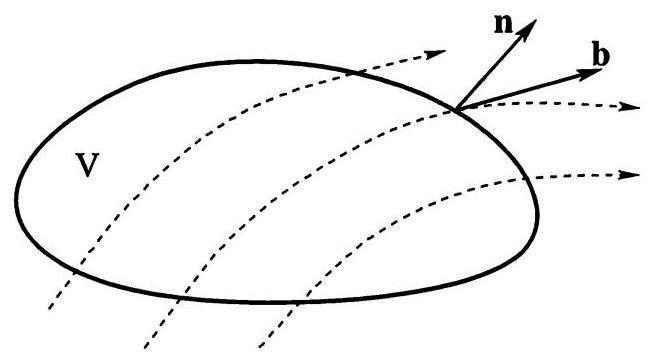
\includegraphics[width=0.6\textwidth]{images/bo_d6ik6nn7aajc739ct1l0_199_417_243_649_359_0.jpg}
\caption{化学物质穿过 $V$ 边界输运时，$V$ 内部所含总量随时间变化.}
\label{fig:linpde-9-1-1}
\end{figure}

利用散度定理，由\eqref{eq:linpde-9-5}可得
\begin{equation}\tag{9.6}\label{eq:linpde-9-6}
{\int }_{V}{u}_{t}{\d x} = {\int }_{V}{a\Delta u\d x} - {\int }_{V}\operatorname{div}\left( {\bm{b}u}\right) {\d x}.
\end{equation}

由于上述恒等式在每个子区域 $V \subset  \Omega$ 上均成立，我们得出 $u = u\left( {t,x}\right)$ 满足抛物型偏微分方程
\[\begin{matrix}
    &{u}_{t}& - &{a\Delta u}&+ &\operatorname{div}\left( {\bm{b}u}\right)&  = &0.\\
    & & & \text{ [扩散]}& & \text{[对流] }& &
\end{matrix}\]


更一般的模型可描述以下情形:

\begin{itemize}\relax
\item\relax 扩散在整个区域上并非均匀:即系数 $a$ 不是常数，而是依赖于位置 $x \in  \Omega$ ；此外，扩散亦非各向同性——在某些方向上比其他方向更快.所有这些可通过将常数扩散矩阵 $A\left( x\right)  \equiv  {aI}$ 替换为更一般的对称矩阵 $A\left( x\right)  = \left( {{a}^{ij}\left( x\right) }\right)$ 来建模.
\end{itemize}

\begin{itemize}\relax
\item\relax $u$ 的总量并不守恒:存在额外项，分别对应线性衰减与外部源.
\end{itemize}

在 $n$ 维空间中，这导出如下形式的线性演化方程\eqref{eq:linpde-9-7}
\begin{equation}\tag{9.7}\label{eq:linpde-9-7}
\begin{matrix} {u}_{t} &  - & \sum_{{i,j = 1}}^{n}{\left( {a}^{ij}\left( x\right) {u}_{{x}_{i}}\right) }_{{x}_{j}} &  + & \sum_{{i = 1}}^{n}{\left( {b}^{i}\left( x\right) u\right) }_{{x}_{i}} &  = &  - c\left( x\right) u &  + & f\left( x\right) \;. \\   & & \text{ [扩散] } & & \text{ [衰减] } & & \text{ [衰减] } & & \text{ [衰减] } \end{matrix}
\end{equation}

方程\eqref{eq:linpde-9-7}可用于建模多种现象，例如质量输运、热传导等.在许多情况下，人们关注稳态解，即与时间无关的解.在\eqref{eq:linpde-9-7}中令 ${u}_{t} = 0$ ，可得线性椭圆型方程
\begin{equation}\tag{9.8}\label{eq:linpde-9-8}
- \sum_{{i,j = 1}}^{n}{\left( {a}^{ij}\left( x\right) {u}_{{x}_{i}}\right) }_{{x}_{j}} + \sum_{{i = 1}}^{n}{\left( {b}^{i}\left( x\right) u\right) }_{{x}_{i}} + c\left( x\right) u = f\left( x\right) .
\end{equation}

\subsection{经典解与弱解}
边界值问题\eqref{eq:linpde-9-2}的经典解是指一个函数 $u \in  {\mathcal{C}}^{2}\left( \Omega \right)$ ，它在每一点均满足方程及边界条件.一般而言，由于方程系数缺乏正则性，问题\eqref{eq:linpde-9-2}可能不存在经典解，因此需引入更弱的解的概念.

\begin{definition}\label{def:linpde-9-2}
\eqref{eq:linpde-9-2}的弱解是一个函数 $u \in  {H}_{0}^{1}\left( \Omega \right)$ ，使得
\begin{equation}\tag{9.9}\label{eq:linpde-9-9}
{\int }_{\Omega }\left( {\sum_{{i,j = 1}}^{n}{a}^{ij}{u}_{{x}_{i}}{v}_{{x}_{j}} - \sum_{{i = 1}}^{n}{b}^{i}u{v}_{{x}_{i}} + {cuv}}\right) {\d x} = {\int }_{\Omega }{fv\d x},\;\forall\,v \in  {H}_{0}^{1}\left( \Omega \right) .
\end{equation}
\end{definition}

\begin{remark}\label{rem:linpde-9-3}
边界条件 $u = 0$ 在 $\partial \Omega$ 上通过要求 $u \in  {H}_{0}^{1}\left( \Omega \right)$ 得以体现.\eqref{eq:linpde-9-9}式形式上由下式经分部积分得到
\begin{equation}\tag{9.10}\label{eq:linpde-9-10}
{\int }_{\Omega }\left( {Lu}\right) {v\d x} = {\int }_{\Omega }{fv\d x}\;\forall\,v \in  {\mathcal{C}}_{c}^{\infty }\left( \Omega \right)
\end{equation}
并分部积分.注意，若\eqref{eq:linpde-9-9}对任意检验函数 $v \in  {\mathcal{C}}_{c}^{\infty }\left( \Omega \right)$ 成立，则通过逼近论证，该积分恒等式对任意 $v \in  {H}_{0}^{1}\left( \Omega \right)$ 仍成立.须特别指出的是，函数 $u \in  {H}_{0}^{1}$ 可能不具有二阶弱导数；但\eqref{eq:linpde-9-9}中的积分对所有 $u,v \in  {H}_{0}^{1}$ 始终良定.
\end{remark}

弱解概念的一种便捷重述方式如下:在Hilbert空间 ${H}_{0}^{1}\left( \Omega \right)$ 上，考虑双线性型
\begin{equation}\tag{9.11}\label{eq:linpde-9-11}
B\left(  {u,v}\right)   \doteq  {\int }_{\Omega }\left( {\sum_{{i,j = 1}}^{n}{a}^{ij}{u}_{{x}_{i}}{v}_{{x}_{j}} - \sum_{{i = 1}}^{n}{b}^{i}u{v}_{{x}_{i}} + {cuv}}\right) {\d x}.
\end{equation}

函数 $u \in  {H}_{0}^{1}$ 是\eqref{eq:linpde-9-2}的弱解，当且仅当
\begin{equation}\tag{9.12}\label{eq:linpde-9-12}
B\left(  {u,v}\right)   = {\left( f,v\right) }_{{L}^{2}},\;\forall\,v \in  {H}_{0}^{1}.
\end{equation}

此处及后文，我们采用记号
\begin{equation}\tag{9.13}\label{eq:linpde-9-13}
{\left( f,g\right) }_{{L}^{2}} \doteq  {\int }_{\Omega }{fg\d x}
\end{equation}
表示 ${L}^{2}\left( \Omega \right)$ 中的内积，以区别于 ${H}^{1}\left( \Omega \right)$ 中的内积
\begin{equation}\tag{9.14}\label{eq:linpde-9-14}
{\left( f,g\right) }_{{H}^{1}} \doteq  {\int }_{\Omega }{fg\d x} + {\int }_{\Omega }\sum_{{i = 1}}^{n}{f}_{{x}_{i}}{g}_{{x}_{i}}{\d x}.
\end{equation}

\begin{remark}\label{rem:linpde-9-4}
方程\eqref{eq:linpde-9-1}中二阶项前的负号，在经形式分部积分后，在\eqref{eq:linpde-9-11}中消失.

后文将明确表明，该符号之选取旨在使相应二次型 $B\left(  {u,v}\right)$ 可为正定.
\end{remark}

\begin{remark}\label{rem:linpde-9-5}
给定函数 $g \in \; {H}^{1}\left( \Omega \right)$ ，可考虑非齐次边值问题
\begin{equation}\tag{9.15}\label{eq:linpde-9-15}
\begin{cases} {Lu} = f,  & x \in  \Omega , \\  u = g, & x \in  \partial \Omega . \end{cases}
\end{equation}

该问题可重写为关于函数 $\widetilde{u} \doteq  u - g$ 的齐次问题，即
\begin{equation}\tag{9.16}\label{eq:linpde-9-16}
\begin{cases} L\widetilde{u} = f - {Lg}, & x \in  \Omega , \\  \widetilde{u} = 0, & x \in  \partial \Omega . \end{cases}
\end{equation}

假设 ${Lg} \in  {L}^{2}\left( \Omega \right)$ ，则问题\eqref{eq:linpde-9-16}与\eqref{eq:linpde-9-2}完全属于同一类型.
\end{remark}

\begin{remark}\label{rem:linpde-9-6}
形如
\[
{Lu} \doteq   - \sum_{{i,j = 1}}^{n}{a}^{ij}\left( x\right) {u}_{{x}_{i}{x}_{j}} + \sum_{{i = 1}}^{n}{b}^{i}\left( x\right) {u}_{{x}_{i}} + c\left( x\right) u
\]
的微分算子可重写为
\[
{Lu} =  - \sum_{{i,j = 1}}^{n}{\left( {a}^{ij}\left( x\right) {u}_{{x}_{i}}\right) }_{{x}_{j}} + \sum_{{i = 1}}^{n}\left( {{b}^{i}\left( x\right)  + \sum_{{j = 1}}^{n}{a}^{ij}{}_{{x}_{j}}\left( x\right) }\right) {u}_{{x}_{i}} + c\left( x\right) u.
\]

假设 ${a}^{ij},{a}^{ij}{}_{{x}_{j}},{b}^{i},c \in  {L}^{\infty }\left( \Omega \right)$ ，相应问题\eqref{eq:linpde-9-2}的弱解仍可通过求解\eqref{eq:linpde-9-12}得到，其中双线性型 $B$ 现定义为
\[
B\left(  {u,v}\right)   \doteq  {\int }_{\Omega }\left( {\sum_{{i,j = 1}}^{n}{a}^{ij}{u}_{{x}_{i}}{v}_{{x}_{j}} + \sum_{{i = 1}}^{n}\left( {{b}^{i} + \sum_{{j = 1}}^{n}{a}^{ij}}\right) {u}_{{x}_{i}}v + {cuv}}\right) {\d x}.
\]
\end{remark}

作为第一个例子，考虑边值问题
\begin{equation}\tag{9.17}\label{eq:linpde-9-17}
\begin{cases}  - {\Delta u} + u   = f, & x \in  \Omega , \\[-3pt]  u  = 0, & x \in  \partial \Omega . \end{cases}
\end{equation}

显然，算子 $- {\Delta u} \doteq   - \sum_{i}{u}_{{x}_{i}{x}_{i}}$ 是一致椭圆的，因为此时 $n \times  n$ 矩阵 $A\left( x\right)  = \left( {{a}^{ij}\left( x\right) }\right)$ 对每个 $x \in  \Omega$ 均为单位矩阵.问题\eqref{eq:linpde-9-17}弱解的存在性可通过基于Riesz表示定理的一个极为简洁的论证予以证明.

\begin{lemma}\label{lem:linpde-9-7}
设 $\Omega  \subset  {\mathbb{R}}^{n}$ 为有界开集.则对任意 $f \in  {L}^{2}\left( \Omega \right)$ ，边值问题\eqref{eq:linpde-9-17}存在唯一弱解 $u \in  {H}_{0}^{1}\left( \Omega \right)$ .相应的映射 $f \mapsto  u$ 是从 ${L}^{2}\left( \Omega \right)$ 到 ${H}_{0}^{1}\left( \Omega \right)$ 的紧线性算子.
\end{lemma}

\begin{proof}
由Rellich-Kondrachov定理，标准嵌入 $\iota$ : ${H}_{0}^{1}\left( \Omega \right)  \mapsto  {L}^{2}\left( \Omega \right)$ 是紧的.故其对偶算子 ${\iota }^{ * }$为紧算子.由于 ${H}_{0}^{1}$ 与 ${L}^{2}$ 均为Hilbert空间，故可与其对偶空间恒等.由此得到:
\begin{equation}\tag{9.18}\label{eq:linpde-9-18}
\setjot[-2]\begin{aligned}
{H}_{0}^{1}\left( \Omega \right) &\overset{\iota }{ \rightarrow  }{L}^{2}\left( \Omega \right)\\
{H}_{0}^{1}\left( \Omega \right)  = {\left(  {H}_{0}^{1}\left( \Omega \right) \right)  }^{ * } &\overset{{\iota }^{ * }}{ \leftarrow  }{\left(  {L}^{2}\left( \Omega \right) \right)  }^{ * } = {L}^{2}\left( \Omega \right) .
\end{aligned}
\end{equation}

对每个 $f \in  {L}^{2}\left( \Omega \right)$ ，由对偶算子定义可得
\[
{\left( {\iota }^{ * }f,v\right) }_{{H}^{1}} = {\left( f,\iota v\right) }_{{L}^{2}} = {\left( f,v\right) }_{{L}^{2}}\;\forall\,f \in  {L}^{2}\left( \Omega \right) ,v \in  {H}_{0}^{1}\left( \Omega \right) .
\]

由\eqref{eq:linpde-9-14}可知， ${\iota }^{ * }f$ 恰为\eqref{eq:linpde-9-17}的弱解.
\end{proof}


\subsection{齐次二阶椭圆算子}
我们首先研究椭圆边值问题
\begin{equation}\tag{9.19}\label{eq:linpde-9-19}
\begin{cases} {Lu}  = f, & x \in  \Omega , \\[-3pt]  u = 0, & x \in  \partial \Omega , \end{cases}
\end{equation}
的解，其中微分算子 $L$ 仅含二阶项:
\begin{equation}\tag{9.20}\label{eq:linpde-9-20}
{Lu} \doteq   - \sum_{{i,j = 1}}^{n}{\left( {a}^{ij}\left( x\right) {u}_{{x}_{i}}\right) }_{{x}_{j}}.
\end{equation}

我们回顾:\eqref{eq:linpde-9-19}的弱解是指满足下式的函数 $u \in  {H}_{0}^{1}\left( \Omega \right)$
\begin{equation}\tag{9.21}\label{eq:linpde-9-21}
B\left(  {u,v}\right)   = {\left( f,v\right) }_{{L}^{2}}\;\forall\,v \in  {H}_{0}^{1}\left( \Omega \right) ,
\end{equation}
其中 $B : {H}_{0}^{1} \times  {H}_{0}^{1} \mapsto  \mathbb{R}$ 是连续双线性型
\begin{equation}\tag{9.22}\label{eq:linpde-9-22}
B\left(  {u,v}\right)   \doteq  {\int }_{\Omega }\sum_{{i,j = 1}}^{n}{a}^{ij}{u}_{{x}_{i}}{v}_{{x}_{j}}{\d x}.
\end{equation}

\begin{theorem}\label{thm:linpde-9-8}
设 $\Omega  \subset  {\mathbb{R}}^{n}$ 为有界开集.设\eqref{eq:linpde-9-20}中的算子 $L$ 一致椭圆，其系数为 ${a}^{ij} \in  {L}^{\infty }\left( \Omega \right)$ .则对任意 $f \in  {L}^{2}\left( \Omega \right)$ ，边值问题\eqref{eq:linpde-9-19}存在唯一弱解 $u \in  {H}_{0}^{1}\left( \Omega \right)$ .相应的解算子(记为 ${L}^{-1} : f \mapsto  u$ )是从 ${L}^{2}\left( \Omega \right)$ 到 ${H}_{0}^{1}\left( \Omega \right)$ 的紧线性算子.
\end{theorem}

\begin{proof}
椭圆边值问题\eqref{eq:linpde-9-19}弱解的存在性与唯一性，可通过验证双线性型 $B$ (见\eqref{eq:linpde-9-22})满足 Lax-Milgram 定理的所有条件而得到.

\noindent 1. $B$ 的连续性显然成立.事实上，
{\setjot[-2]\begin{align*}
    \left| {B\left(  {u,v}\right)  }\right|  &\leq  \sum_{{i,j = 1}}^{n}{\int }_{\Omega }\left| {{a}^{ij}{u}_{{x}_{i}}{v}_{{x}_{j}}}\right| {\d x} \leq  \sum_{{i,j = 1}}^{n}{\norm{a}^{ij}}_{{L}^{\infty }}{\norm{u}_{{x}_{i}}}_{{L}^{2}}{\norm{v}_{{x}_{j}}}_{{L}^{2}}\\
    &\leq  C\| u{\| }_{{H}^{1}}\| v{\| }_{{H}^{1}}
\end{align*}}

\noindent 2. 我们断言 $B$ 是严格正定的，即存在 $\beta  > 0$ ，使得
\begin{equation}\tag{9.23}\label{eq:linpde-9-23}
B\left(  {u,u}\right)  \; \geq  \;\beta \| u{\| }_{{H}^{1}\left( \Omega \right) }^{2}\;\forall\,u \in  {H}_{0}^{1}\left( \Omega \right) \;.
\end{equation}

事实上，由于 $\Omega$ 有界，Poincaré 不等式保证存在常数 $\kappa$ ，使得
\[
\| u{\| }_{{L}^{2}\left( \Omega \right) }^{2} \leq  \kappa {\int }_{\Omega }{\left| \nabla u\right| }^{2}{\d x}\;\forall\,u \in  {H}_{0}^{1}\left( \Omega \right) .
\]

另一方面，一致椭圆性条件蕴含
\[
B\left(  {u,u}\right)   = {\int }_{\Omega }\sum_{{i,j = 1}}^{n}{a}^{ij}{u}_{{x}_{i}}{u}_{{x}_{j}}{\d x} \geq  {\int }_{\Omega }\theta \sum_{{i = 1}}^{n}{u}_{{x}_{i}}^{2}{\d x} = \theta {\int }_{\Omega }{\left| \nabla u\right| }^{2}{\d x}.
\]

上述两个不等式联立可得
\[
\| u{\| }_{{H}^{1}}^{2} = \| u{\| }_{{L}^{2}}^{2} + \| \nabla u{\| }_{{L}^{2}}^{2} \leq  \left( {\kappa  + 1}\right) \| \nabla u{\| }_{{L}^{2}}^{2} \leq  \frac{\kappa  + 1}{\theta }B\left(  {u,u}\right)  .
\]

这证明了\eqref{eq:linpde-9-23}，其中 $\beta  = \theta /\left( {\kappa  + 1}\right)$ .

\noindent 3. 由 Lax-Milgram 定理，对任意 $\widetilde{f} \in  {H}_{0}^{1}\left( \Omega \right)$ ，存在唯一元素 $u \in  {H}_{0}^{1}$ ，使得
\begin{equation}\tag{9.24}\label{eq:linpde-9-24}
B\left(  {u,v}\right)   = {\left( \widetilde{f},v\right) }_{{H}^{1}}\;\forall\,v \in  {H}_{0}^{1}\left( \Omega \right) .
\end{equation}

此外，映射 $\Lambda  : \widetilde{f} \mapsto  u$ 连续，即
\[
\| u{\| }_{{H}^{1}} \leq  {\beta }^{-1}\| \widetilde{f}{\| }_{{H}^{1}}.
\]

取\eqref{eq:linpde-9-18}中定义的 $\widetilde{f} \doteq  {\iota }^{ * }f \in  {H}_{0}^{1}\left( \Omega \right)$ ，从而得到
\begin{equation}\tag{9.25}\label{eq:linpde-9-25}
B\left(  {u,v}\right)   = {\left( {\iota }^{ * }f,v\right) }_{{H}^{1}} = {\left( f,v\right) }_{{L}^{2}}\;\forall\,v \in  {H}_{0}^{1}\left( \Omega \right) .
\end{equation}

依定义， $u$ 是\eqref{eq:linpde-9-19}的弱解.

\noindent 4. 为证解算子 ${L}^{-1} : f \mapsto  u$ 是紧的，考虑如下图示
\[
{L}^{2}\left( \Omega \right) \overset{{\iota }^{ * }}{ \rightarrow  }{H}_{0}^{1}\left( \Omega \right) \overset{\Lambda }{ \rightarrow  }{H}_{0}^{1}\left( \Omega \right) .
\]

由引理\ref{lem:linpde-9-7}，线性算子${\iota }^{ * }$紧，且 $\Lambda$ 连续.因此复合算子${L}^{-1} = \Lambda  \circ  {\iota }^{ * }$ 是紧的.
\end{proof}

\subsection{按特征函数的展开表示}
由于 ${H}_{0}^{1}\left( \Omega \right)  \subset  {L}^{2}\left( \Omega \right)$ ，定理 9.8 所述的解算子 ${L}^{-1}$ 亦可视为从 ${L}^{2}\left( \Omega \right)$ 到其自身的紧算子.在对称情形 ${a}^{ij} = {a}^{ji}$ 下，算子 ${L}^{-1}$ 是自伴的.故由 Hilbert-Schmidt 定理，它可按一列可数的特征函数基展开表示.
\begin{theorem}\label{thm:linpde-9-9}
假设 ${a}^{ij} = {a}^{ji} \in  {L}^{\infty }\left( \Omega \right)$ .则在定理\ref{thm:linpde-9-8}的设定下，线性算子 ${L}^{-1} : {L}^{2}\left( \Omega \right)  \mapsto  {L}^{2}\left( \Omega \right)$ 是紧的、单射的且自伴的.

空间 ${L}^{2}\left( \Omega \right)$ 具有由 ${L}^{-1}$ 的特征函数构成的可数标准正交基 $\left\{  {{\phi }_{k};k \geq  1}\right\}$ ，且有如下表示
\begin{equation}\tag{9.26}\label{eq:linpde-9-26}
{L}^{-1}f = \sum_{{k = 1}}^{\infty }{\lambda }_{k}{\left( f,{\phi }_{k}\right) }_{{L}^{2}}{\phi }_{k}
\end{equation}
相应的特征值 ${\lambda }_{k}$ 满足
\begin{equation}\tag{9.27}\label{eq:linpde-9-27}
\mathop{\lim }\limits_{{k \rightarrow  \infty }}{\lambda }_{k} = 0,\;{\lambda }_{k} > 0\forall\,k \geq  1.
\end{equation}
\end{theorem}

\begin{proof}
1. 由定理\ref{thm:linpde-9-8}可知， ${L}^{-1}$ 是从 ${L}^{2}\left( \Omega \right)$ 到其自身的紧线性算子.

为证 ${L}^{-1}$ 是单射，假设 $u = {L}^{-1}f = 0$ .则
\[
0 = B\left(  {u,v}\right)   = {\left( f,v\right) }_{{L}^{2}}
\]
对每个 $v \in  {H}_{0}^{1}\left( \Omega \right)$ 成立.特别地，对每个检验函数 $\phi  \in  {\mathcal{C}}_{c}^{\infty }\left( \Omega \right)$ ，有
\[
{\int }_{\Omega }{f\phi \d x} = 0.
\]
这意味着 $f\left( x\right)  = 0$几乎处处成立于$x \in  \Omega$ .故 $\operatorname{Ker}\left( {L}^{-1}\right)  = \{ 0\}$ ，且${L}^{-1}$ 是单射.

2. 为证 ${L}^{-1}$ 是自伴的，假设
\[
f,g \in  {L}^{2}\left( \Omega \right) ,\;u = {L}^{-1}f,\;v = {L}^{-1}g.
\]

由\eqref{eq:linpde-9-21}中弱解的定义，这蕴含 $u,v \in  {H}_{0}^{1}\left( \Omega \right)$ 且
\[
{\left( {L}^{-1}f,g\right) }_{{L}^{2}} = {\int }_{\Omega }{ug\d x} = {\int }_{\Omega }\sum_{{i,j}}{a}^{ij}{u}_{{x}_{i}}{v}_{{x}_{j}}{\d x} = {\int }_{\Omega }{fv\d x} = {\left( f,{L}^{-1}g\right) }_{{L}^{2}}.
\]

注意第二个等式成立是因为 $v = {L}^{-1}g$ ，其中以 $u \in  {H}_{0}^{1}\left( \Omega \right)$ 作为检验函数；第三个等式成立是因为 $u = {L}^{-1}f$ ，其中以 $v \in  {H}_{0}^{1}\left( \Omega \right)$ 作为检验函数.

3. 由于 ${L}^{-1}$ 是可分空间 ${L}^{2}\left( \Omega \right)$ 上的紧自伴算子，根据第6章的Hilbert-Schmidt定理，存在由 ${L}^{-1}$ 的特征函数构成的可数标准正交基.由此得到\eqref{eq:linpde-9-26}.

由算子 ${L}^{-1}$ 的紧性，其特征值满足 ${\lambda }_{k} \rightarrow  0$ .最后，在\eqref{eq:linpde-9-21}中取 $v = {\phi }_{k}$ 为检验函数，可得
\[
B\left(  {{\lambda }_{k}{\phi }_{k},{\phi }_{k}}\right)   = {\left( {\phi }_{k},{\phi }_{k}\right) }_{{L}^{2}} = 1.
\]

由于二次型 $B$ 是严格正定的，我们得出
\[
{\lambda }_{k} = \frac{1}{B\left(  {{\phi }_{k},{\phi }_{k}}\right)  } > 0.
\]
\end{proof}

\begin{instance}\label{ins:linpde-9-10}
设 $\Omega  \doteq  ( 0,\pi \left(  { \subset  \mathbb{R}}\right.$ 和 ${Lu} =  - {u}_{xx}$ .给定 $f \in  {L}^{2}\left( {( 0,\pi ) }\right)$ ，考虑椭圆边值问题
\begin{equation}\tag{9.28}\label{eq:linpde-9-28}
\begin{cases}  - {u}_{xx} &  = f,\;0 < x < \pi , \\  u\left( 0\right) &  = u\left( \pi \right)  = 0. \end{cases}
\end{equation}

第一步，我们计算算子 ${Lu} =  - {u}_{xx}$ 的特征函数.求解边值问题
\[
- {u}_{xx} = {\mu u},\;u\left( 0\right)  = u\left( \pi \right)  = 0,
\]

可得特征值及归一化特征函数
\[
{\mu }_{k} = {k}^{2},\;{\phi }_{k}\left( x\right)  = \sqrt{\frac{2}{\pi }}\sin {kx}.
\]

显然，逆算子 ${L}^{-1}$ 具有相同的特征函数 ${\phi }_{k}$ ，对应特征值为 ${\lambda }_{k} = 1/{k}^{2}$ .

在此特殊情形下，公式\eqref{eq:linpde-9-26}给出\eqref{eq:linpde-9-28}之解的著名Fourier正弦级数表示:
{\begin{align*}
    u\left( x\right)  &= {L}^{-1}f = \sum_{{k = 1}}^{\infty }{\lambda }_{k}{\left( f,{\phi }_{k}\right) }_{{L}^{2}}{\phi }_{k}\\
    &= \sum_{{k = 1}}^{\infty }\frac{1}{{k}^{2}}\left( {{\int }_{0}^{\pi }f\left( y\right) \sqrt{\frac{2}{\pi }}\sin {ky\d y}}\right) \sqrt{\frac{2}{\pi }}\sin {kx}\\
    &= \sum_{{k = 1}}^{\infty }\frac{2}{\pi {k}^{2}}\left( {{\int }_{0}^{\pi }f\left( y\right) \sin {ky\d y}}\right) \sin {kx}.
\end{align*}}

\end{instance}

\subsection{更一般的线性椭圆型算子}
定理\ref{thm:linpde-9-8}中所述的存在唯一性结果依赖于双线性型 $B$ 在空间 ${H}_{0}^{1}\left( \Omega \right)$ 上的严格正定性(见\eqref{eq:linpde-9-21}).该性质对更一般的双线性型 $B$ (见\eqref{eq:linpde-9-11})不再成立，因其含附加的低阶项.例如，若函数 $c\left( x\right)$ 取绝对值很大的负值，则可能存在某个 $u \in  {H}_{0}^{1}\left( \Omega \right)$ ，使得 $B\left(  {u,u}\right)   < 0.$

\begin{instance}\label{ins:linpde-9-11}
考虑开区间 $\Omega  \doteq  ( 0,\pi )$ .注意到该算子
\[
{Lu} \doteq   - {u}_{xx} - {4u}
\]

在 $\Omega$ 上是一致椭圆的.然而，对应的双线性形式
\[
B\left(  {u,v}\right)   = {\int }_{0}^{\pi }{u}_{x}{v}_{x} - {4uv\d x}
\]

在 ${H}_{0}^{1}\left( \Omega \right)$ 上并非正定.例如，取 $u\left( x\right)  = \sin x$ ，可得
\[
B\left(  {u,u}\right)   = {\int }_{0}^{\pi }{\cos }^{2}x - 4{\sin }^{2}{x\d x} =  - \frac{3\pi }{2}.
\]

若 $f\left( x\right)  = \sin {2x}$ ，则边值问题
\begin{equation}\tag{9.29}\label{eq:linpde-9-29}
\begin{cases}  - {u}_{xx} - {4u} = \sin {2x},\; x \in  ( 0,\pi ) \\  u\left( 0\right) = u\left( \pi \right)  = 0 \end{cases}
\end{equation}

无解.事实上，取 $v\left( x\right)  = \sin {2x}$ ，对任意 $u \in  {H}_{0}^{1}\left( \Omega \right)$ ，分部积分可得
{\setjot[-2]\begin{align*}
    B\left({u,v}\right)  &= {\int }_{0}^{\pi }{u}_{x}{v}_{x} - {4uv\d x} = {\int }_{0}^{\pi }\left( {2{u}_{x}\cos {2x} - {4u}\sin {2x}}\right) {\d x}\\
    &= {\int }_{0}^{\pi }{\left( 2u\sin 2x\right) }_{x}{\d x} = 0 \neq  {\int }_{0}^{\pi }{\sin }^{2}{2x\d x} = {\left( f,v\right) }_{{L}^{2}}.
\end{align*}}


因此，不存在满足\eqref{eq:linpde-9-12}的函数 $u \in  {H}_{0}^{1}\left( \Omega \right)$ .

与此相关，还应注意对应的齐次问题
\begin{equation}\tag{9.30}\label{eq:linpde-9-30}
\begin{cases}  - {u}_{xx} - {4u} &  = 0,\;x \in  ( 0,\pi ) \\  u\left( 0\right) &  = u\left( \pi \right)  = 0 \end{cases}
\end{equation}
具有无穷多个解: $u\left( x\right)  = \kappa \sin {2x}$ ，其中 $\kappa$ 为任意常数.
\end{instance}

接下来，我们研究更一般的边值问题\eqref{eq:linpde-9-1}--\eqref{eq:linpde-9-2}的弱解的存在性与唯一性.我们的方法分为两个步骤.

第一步:选取足够大的常数 $\gamma  > 0$ ，使得算子
\begin{equation}\tag{9.31}\label{eq:linpde-9-31}
{L}_{\gamma }u \doteq  {Lu} + {\gamma u}
\end{equation}

严格正定.更准确地说，对应的双线性形式\eqref{eq:linpde-9-32}满足\eqref{eq:linpde-9-33}的估计：
\begin{gather}\tag{9.32}\label{eq:linpde-9-32}
    {B}_{\gamma }\left(  {u,v}\right)   \doteq  {\int }_{\Omega }\left( {\sum_{{i,j = 1}}^{n}{a}^{ij}\left( x\right) {u}_{{x}_{i}}{v}_{{x}_{j}} - \sum_{{i = 1}}^{n}{b}^{i}\left( x\right) u{v}_{{x}_{i}} + \mathrm{c}\left( x\right) {uv} + {\gamma uv}}\right) {\d x} \\ \label{eq:linpde-9-33}
{B}_{\gamma }\left(  {u,u}\right)   \geq  \beta \| u{\| }_{{H}^{1}}^{2}\;\forall\,u \in  {H}_{0}^{1}\left( \Omega \right) ,
\end{gather}
其中 $\beta  > 0$ 为某常数.由Lax-Milgram定理可知，对每个 $f \in  {L}^{2}\left( \Omega \right)$ ，方程
\[
{L}_{\gamma }u = f
\]
存在唯一弱解 $u \in  {H}_{0}^{1}\left( \Omega \right)$ .此外，映射 $f \mapsto  u = {L}_{\gamma }^{-1}f$ 是从 ${L}^{2}\left( \Omega \right)$ 到 ${H}_{0}^{1}\left( \Omega \right)  \subset  {L}^{2}\left( \Omega \right)$ 的线性紧算子.我们将 ${L}_{\gamma }^{-1}$ 视为从 ${L}^{2}\left( \Omega \right)$ 到其自身的紧算子.

第二步:原问题\eqref{eq:linpde-9-2}现可写为
\[
{Lu} = {L}_{\gamma }u - {\gamma u} = f.
\]

将算子 ${L}_{\gamma }^{-1}$ 作用于等式两边，可得
\begin{equation}\tag{9.34}\label{eq:linpde-9-34}
u - {L}_{\gamma }^{-1}{\gamma u} = {L}_{\gamma }^{-1}f
\end{equation}

引入记号
\begin{equation}\tag{9.35}\label{eq:linpde-9-35}
K \doteq  \gamma {L}_{\gamma }^{-1},\;h \doteq  {L}_{\gamma }^{-1}f,
\end{equation}

我们导出方程
\begin{equation}\tag{9.36}\label{eq:linpde-9-36}
\left( {I - K}\right) u = h
\end{equation}

由于 $K$ 是从 ${L}^{2}\left( \Omega \right)$ 到自身的紧算子，可应用Fredholm理论.特别地，有Fredholm择一性：要么(i)对每个 $h \in  {L}^{2}\left( \Omega \right)$ ，方程 $u - {Ku} = h$ 存在唯一解 $u \in  {L}^{2}\left( \Omega \right)$，否则(ii)方程 $u - {Ku} = 0$ 存在非平凡解 $u \in  {L}^{2}\left( \Omega \right)$.

记 ${K}^{ * } : {L}^{2} \mapsto  {L}^{2}$ 为伴随算子，则情形(ii)成立当且仅当伴随方程 $v - {K}^{ * }v = 0$ 存在非平凡解 $v \in  {L}^{2}\left( \Omega \right)$ .因此，关于\eqref{eq:linpde-9-2}式弱解的存在性与唯一性的信息，亦可通过研究伴随算子获得
\begin{equation}\tag{9.37}\label{eq:linpde-9-37}
{L}^{ * }v \doteq   - \sum_{{i,j = 1}}^{n}{\left( {a}^{ij}\left( x\right) {v}_{{x}_{j}}\right) }_{{x}_{i}} - \sum_{{i = 1}}^{n}{b}^{i}\left( x\right) {v}_{{x}_{i}} + c\left( x\right) v.
\end{equation}

本节余下部分将给出上述断言的详细证明.

\begin{lemma}\label{lem:linpde-9-12}
设\eqref{eq:linpde-9-1}式中的算子 $L$ 是一致椭圆的，其系数为 ${a}^{ij},{b}^{i},\mathrm{c} \in  {L}^{\infty }\left( \Omega \right)$ .则存在常数 $\alpha ,\beta ,\gamma  > 0$ ，使得对所有 $u,v \in  {H}_{0}^{1}\left( \Omega \right)$ 成立：
\begin{gather}\tag{9.38}\label{eq:linpde-9-38}
    \left| {B\left(  {u,v}\right)  }\right|  \leq  \alpha \| u{\| }_{{H}^{1}}\| v{\| }_{{H}^{1}}, \\ \tag{9.39}\label{eq:linpde-9-39}
    \beta \| u{\| }_{{H}^{1}}^{2} \leq  B\left(  {u,u}\right)   + \gamma \| u{\| }_{{L}^{2}}^{2}. 
\end{gather}
\end{lemma}

\begin{proof}
1. 双线性型 $B : {H}_{0}^{1} \times  {H}_{0}^{1} \mapsto  \mathbb{R}$ 的有界性由下式推出
{\setjot[-2]\begin{align*}
    \left| {B\left(  {u,v}\right)  }\right|  &= \left| {{\int }_{\Omega }\left( {\sum_{{i,j = 1}}^{n}{a}^{ij}{u}_{{x}_{i}}{v}_{{x}_{j}} - \sum_{{i = 1}}^{n}{b}^{i}u{v}_{{x}_{i}} + {cuv}}\right) {\d x}}\right|\\
    &\leq  \sum_{{i,j = 1}}^{n}{\norm{a}^{ij}}_{{L}^{\infty }}{\norm{u}_{{x}_{i}}}_{{L}^{2}}{\norm{v}_{{x}_{j}}}_{{L}^{2}} + \sum_{{i = 1}}^{n}{\norm{b}^{i}}_{{L}^{\infty }}\| u{\| }_{{L}^{2}}{\norm{v}_{{x}_{i}}}_{{L}^{2}}\\
    &\quad + \| \mathrm{c}{\| }_{{L}^{\infty }}\| u{\| }_{{L}^{2}}\| v{\| }_{{L}^{2}}\\
    &\leq  \alpha \| u{\| }_{{H}^{1}}\| v{\| }_{{H}^{1}}
\end{align*}}

\noindent 2. 关于第二个估计，利用椭圆性条件\eqref{eq:linpde-9-4}及初等不等式 ${ab} \leq  \frac{1}{2\theta }{a}^{2} + \frac{\theta }{2}{b}^{2}$ ，得到
{\setjot[-2]\begin{align*}
    \theta \sum_{{i = 1}}^{n}{\norm{u}_{{x}_{i}}}_{{L}^{2}}^{2} &= \theta {\int }_{\Omega }\sum_{{i = 1}}^{n}{u}_{{x}_{i}}^{2}{\d x} \leq  {\int }_{\Omega }\sum_{{i,j = 1}}^{n}{a}^{ij}{u}_{{x}_{i}}{u}_{{x}_{j}}{\d x}\\
    &= B\left(  {u,u}\right)   + {\int }_{\Omega }\left( {\sum_{{i = 1}}^{n}{b}^{i}u{u}_{{x}_{i}} - c{u}^{2}}\right) {\d x}\\
    &\leq  B\left(  {u,u}\right)   + \sum_{{i = 1}}^{n}{\norm{b}^{i}}_{{L}^{\infty }}\| u{\| }_{{L}^{2}}{\norm{u}_{{x}_{i}}}_{{L}^{2}} + \| c{\| }_{{L}^{\infty }}\| u{\| }_{{L}^{2}}^{2}\\
    &\leq  B\left(  {u,u}\right)   + \left( {\frac{1}{2\theta }\sum_{{i = 1}}^{n}{\norm{b}^{i}}_{{L}^{\infty }}^{2}\| u{\| }_{{L}^{2}}^{2} + \frac{\theta }{2}\sum_{{i = 1}}^{n}{\norm{u}_{{x}_{i}}}_{{L}^{2}}^{2}}\right)  + \| c{\| }_{{L}^{\infty }}\| u{\| }_{{L}^{2}}^{2}.
\end{align*}}

因此
\[
B\left(  {u,u}\right)   \geq  \frac{\theta }{2}\sum_{{i = 1}}^{n}{\norm{u}_{{x}_{i}}}_{{L}^{2}}^{2} - C\| u{\| }_{{L}^{2}}^{2}\;\forall\,u \in  {H}_{0}^{1}\left( \Omega \right) ,
\]
对某个适当常数 $C$ 成立.取 $\beta  = \theta /2$ 和 $\gamma  = C + \theta /2$ ，不等式\eqref{eq:linpde-9-39}即得满足.
\end{proof}

\begin{remark}\label{rem:linpde-9-13}
由上述引理可知，若常数 $\gamma  > 0$ 足够大，则该双线性型
\[
{B}_{\gamma }\left(  {u,v}\right)   \doteq  B\left(  {u,v}\right)   + \gamma {\left( u,v\right) }_{{L}^{2}}
\]

在\eqref{eq:linpde-9-32}中是严格正定的.注意，若 $\gamma  > 0$ 充分大，则极易证明该双线性形式
\[
{\widetilde{B}}_{\gamma } \doteq  B\left(  {u,v}\right)   + \gamma {\left( u,v\right) }_{{H}^{1}}
\]

在 ${H}_{0}^{1}\left( \Omega \right)$ 上严格正定.然而，引理\ref{lem:linpde-9-12}表明，我们可通过添加弱得多的项 $\gamma {\left( u,v\right) }_{{L}^{2}}$ 来实现严格正定性.

令 $\gamma$ 如\eqref{eq:linpde-9-39}所定义，并按\eqref{eq:linpde-9-32}定义双线性形式 ${B}_{\gamma }$ .由于 ${B}_{\gamma }$ 严格正定，可应用Lax-Milgram定理，从而得出:对任意 $f \in  {L}^{2}\left( \Omega \right)$ ，存在唯一的 $u \in  {H}_{0}^{1}\left( \Omega \right)$ 使得
\begin{equation}\tag{9.40}\label{eq:linpde-9-40}
{B}_{\gamma }\left(  {u,v}\right)   = {\left( f,v\right) }_{{L}^{2}} = {\left( {\iota }^{ * }f,v\right) }_{{H}^{1}}\;\forall\,v \in  {H}_{0}^{1}\left( \Omega \right) .
\end{equation}

由于映射 ${\iota }^{ * }$ 是紧的，解算子 $f \mapsto  u = {L}_{\gamma }^{-1}f$ 是从 ${L}^{2}\left( \Omega \right)$ 到 ${H}_{0}^{1}\left( \Omega \right)$ 的线性紧算子.因此，它也是从 ${L}^{2}\left( \Omega \right)$ 到其自身的紧算子.

对伴随问题，存在完全类似的结果
\begin{equation}\tag{9.41}\label{eq:linpde-9-41}
\left\{  \begin{aligned} {L}_{\gamma }^{ * }v &  = g, & & x \in  \Omega , \\  v &  = 0, & & x \in  \partial \Omega , \end{aligned}\right.
\end{equation}

其中 ${L}^{ * }$ 为\eqref{eq:linpde-9-37}中引入的伴随算子， ${L}_{\gamma }^{ * }u \doteq  {L}^{ * }u + {\gamma u}$ .给定 $g \in  {L}^{2}\left( \Omega \right)$ ，\eqref{eq:linpde-9-41}的弱解定义为满足下式的函数 $v \in  {H}_{0}^{1}\left( \Omega \right)$
\begin{equation}\tag{9.42}\label{eq:linpde-9-42}
{B}_{\gamma }^{ * }\left(  {v,u}\right)   \doteq  {B}_{\gamma }\left(  {u,v}\right)   = {\left( u,g\right) }_{{L}^{2}}\;\forall\,u \in  {H}_{0}^{1}\left( \Omega \right) .
\end{equation}

由于 ${B}_{\gamma }^{ * }$ 严格正定，故对任意 $g \in  {L}^{2}$ ，Lax-Milgram定理保证\eqref{eq:linpde-9-41}存在唯一弱解 $v$ .映射 $g \mapsto  v = \; {\left( {L}_{\gamma }^{ * }\right) }^{-1}g$ 是从 ${L}^{2}\left( \Omega \right)$ 到其自身的线性紧算子.
\end{remark}

\begin{lemma}\label{lem:linpde-9-14}
在上述设定下，算子 ${\left( {L}_{\gamma }^{ * }\right) }^{-1}$ 是算子 ${L}_{\gamma }^{-1}$ 的伴随算子.
\end{lemma}

\begin{proof}
由定义，对任意 $f,g \in  {L}^{2}\left( \Omega \right)$ 和 $u,v \in  {H}_{0}^{1}\left( \Omega \right)$ ，有
\[
{\left( f,v\right) }_{{L}^{2}} = {B}_{\gamma }\left(  {{L}_{\gamma }^{-1}f,v}\right)  ,\;{\left( u,g\right) }_{{L}^{2}} = {B}_{\gamma }\left(  {u,{\left( {L}_{\gamma }^{-1}\right) }^{ * }g}\right)  .
\]

特别地，取 $v = {\left( {L}_{\gamma }^{ * }\right) }^{-1}g$ 和 $u = {L}_{\gamma }^{-1}f$ ，可得
\[
{\left( f,{\left( {L}_{\gamma }^{ * }\right) }^{-1}g\right) }_{{L}^{2}} = {B}_{\gamma }\left(  {{L}_{\gamma }^{-1}f,{\left( {L}_{\gamma }^{-1}\right) }^{ * }g}\right)   = {\left( {L}_{\gamma }^{-1}f,g\right) }_{{L}^{2}}.\qedhere
\]
\end{proof}

\begin{lemma}\label{lem:linpde-9-15}
对任意 $f \in \; {L}^{2}\left( \Omega \right)$ ，函数 $u \in  {L}^{2}\left( \Omega \right)$ 是\eqref{eq:linpde-9-2}的弱解当且仅当
\begin{equation}\tag{9.43}\label{eq:linpde-9-43}
\left( {I - K}\right) u = h,\;\text{其中}\;K = \gamma {L}_{\gamma }^{-1},\;h = {L}_{\gamma }^{-1}f.
\end{equation}
\end{lemma}

\begin{proof}
1. 设 $u$ 是\eqref{eq:linpde-9-2}的弱解.由定义，这意味着 $u \in  {H}_{0}^{1}\left( \Omega \right)$ 且
\[
{B}_{\gamma }\left(  {u,v}\right)   = B\left(  {u,v}\right)   + \gamma {\left( u,v\right) }_{{L}^{2}} = {\left( f + \gamma u,v\right) }_{{L}^{2}}\;\forall\,v \in  {H}_{0}^{1}\left( \Omega \right) .
\]

因此
\[
u = {L}_{\gamma }^{-1}\left( {f + {\gamma u}}\right)  = h + {Ku}.
\]

2. 为证其逆命题，设\eqref{eq:linpde-9-43}成立.则
\[
u = \gamma {L}_{\gamma }^{-1}u + {L}_{\gamma }^{-1}f \in  {H}_{0}^{1}\left( \Omega \right) .
\]

此外，对任意 $v \in  {H}_{0}^{1}\left( \Omega \right)$ ，均有
\[
B\left(  {u,v}\right)   = {B}_{\gamma }\left(  {u,v}\right)   - \gamma {\left( u,v\right) }_{{L}^{2}} = {\left( f + \gamma u,v\right) }_{{L}^{2}} - \gamma {\left( u,v\right) }_{{L}^{2}} = {\left( f,v\right) }_{{L}^{2}}.\qedhere
\]
\end{proof}

为应用Fredholm理论(定理6.1)，我们除\eqref{eq:linpde-9-2}外还考虑齐次问题及其伴随问题
\begin{gather}
\begin{cases} {Lu}  = 0, & x \in  \Omega , \\[-1pt]  u  = 0, & x \in  \partial \Omega , \end{cases} \tag{9.44}\label{eq:linpde-9-44}\\[-5pt]
\tag{9.45}\label{eq:linpde-9-45}
\begin{cases} {L}^{ * }v  = 0,  & x \in  \Omega , \\[-1pt]  v  = 0, & x \in  \partial \Omega , \end{cases}
\end{gather}
其中 ${L}^{ * }$ 是在\eqref{eq:linpde-9-37}处定义的伴随线性算子.

\begin{theorem}\label{thm:linpde-9-16}
在基本假设 (H) 下，下列命题等价:

(i) 对任意 $f \in  {L}^{2}\left( \Omega \right)$ ，椭圆边值问题 \eqref{eq:linpde-9-2} 存在唯一的弱解.

(ii) 齐次边值问题 \eqref{eq:linpde-9-44} 仅有解 $u\left( x\right)  \equiv  0$ .

(iii) 伴随齐次问题 \eqref{eq:linpde-9-45} 仅有解 $v\left( x\right) \; \equiv  0$ .
\end{theorem}

\begin{proof}
1. 由于 $K = \gamma {L}_{\gamma }^{-1}$ 是从 ${L}^{2}\left( \Omega \right)$ 到其自身的紧算子，故可应用 Fredholm 定理.由此可知，线性算子 $I - K$ 是满射当且仅当它是一一的，即当且仅当 $\operatorname{Ker}\left( {I - K}\right)  = \{ 0\}$

\noindent 2. 由引理\ref{lem:linpde-9-15}， $u - {Ku} = 0$ 当且仅当 $u$ 是 \eqref{eq:linpde-9-44} 的弱解.完全类似的论证表明: $v - {K}^{ * }v = 0$ 当且仅当 $v$ 是 \eqref{eq:linpde-9-45} 的弱解.

由 Fredholm 定理， $\operatorname{Ker}\left( {I - K}\right)$ 与 $\operatorname{Ker}\left( {I - {K}^{ * }}\right)$ 具有相同维数.于是我们得到一串等价命题:
{\setjot[-3]\begin{gather*}
    I - K\;\text{是单射, } \\
    \operatorname{Ker}\left( {I - K}\right)  = \{ 0\}\\
    \operatorname{Ker}\left( {I - {K}^{ * }}\right)  = \{ 0\}\\
    u \equiv  0\;\text{是}\;\eqref{eq:linpde-9-44}\;\text{的唯一解, } \\
    v \equiv  0\;\text{是}\;\eqref{eq:linpde-9-45}\;\text{的唯一解. } \qedhere
\end{gather*}}
\end{proof}

定理\ref{thm:linpde-9-16}覆盖了 $I - K$ 是一一的且 Fredholm 第一择一性成立的情形.当 $I - K$ 不一定是一一的情形下，方程
\[
u - {Ku} = {L}_{\gamma }^{-1}f
\]
的解的存在性可借助恒等式
\begin{equation}\tag{9.46}\label{eq:linpde-9-46}
\operatorname{Range}\left( {I - K}\right)  = {\left(  \operatorname{Ker}\left( I - {K}^{ * }\right) \right)  }^{ \bot  }.
\end{equation}

\begin{theorem}\label{thm:linpde-9-17}
在假设 $\left( \bm{H}\right)$ 下，问题\eqref{eq:linpde-9-2}至少存在一个弱解当且仅当
\begin{equation}\tag{9.47}\label{eq:linpde-9-47}
{\left( f,v\right) }_{{L}^{2}} = 0
\end{equation}

对伴随问题\eqref{eq:linpde-9-45}的每个弱解 $v \in  {H}_{0}^{1}\left( \Omega \right)$ 成立.
\end{theorem}

\begin{proof}
边值问题\eqref{eq:linpde-9-2}存在弱解当且仅当 ${L}_{\gamma }^{-1}f \in  \operatorname{Range}\left( {I - K}\right)$ .由\eqref{eq:linpde-9-46}，这成立当且仅当 ${L}_{\gamma }^{-1}f$ 与每个 $v \in  \operatorname{Ker}\left( {I - {K}^{ * }}\right)$ 正交，即与伴随问题\eqref{eq:linpde-9-45}的每个解 $v$ 正交.

我们断言:这成立当且仅当 $f$ 本身与\eqref{eq:linpde-9-45}的每个解 $v$ 正交.事实上，若 $v - {K}^{ * }v = 0$，则有
\[
{\left( f,v\right) }_{{L}^{2}} = {\left( f,{K}^{ * }v\right) }_{{L}^{2}} = {\left( Kf,v\right) }_{{L}^{2}} = \gamma {\left( {L}_{\gamma }^{-1}f,v\right) }_{{L}^{2}}.
\]

由于 $\gamma  > 0$ ，这证明了我们的断言.
\end{proof}

\section{抛物型方程}

设 $\Omega  \subset  {\mathbb{R}}^{n}$ 为有界开集， $L$ 为\eqref{eq:linpde-9-1}中的算子.除本章开头所述的标准假设 (H) 外，我们进一步假设系数 ${a}^{ij}$ 满足更强的正则性条件
\begin{equation}\tag{9.48}\label{eq:linpde-9-48}
{a}^{ij} \in  {W}^{1,\infty }\left( \Omega \right) \text{ . }
\end{equation}

本节研究抛物型初边值问题
\begin{equation}\tag{9.49}\label{eq:linpde-9-49}
\begin{cases} {u}_{t} + {Lu} = 0, &  t > 0,x \in  \Omega , \\[-1pt]  u\left( {t,x}\right)  = 0, & t > 0,x \in  \partial \Omega , \\[-1pt]  u\left( {0,x}\right) = g\left( x\right) , & x \in  \Omega . \end{cases}
\end{equation}

将\eqref{eq:linpde-9-49}重新表述为 Hilbert 空间 $X = {L}^{2}\left( \Omega \right)$ 中的 Cauchy 问题较为方便，即
\begin{equation}\tag{9.50}\label{eq:linpde-9-50}
\frac{d}{\d t}u = {Au},\;u\left( 0\right)  = g,
\end{equation}
其中 $A : {L}^{2}\left( \Omega \right)  \mapsto  {L}^{2}\left( \Omega \right)$ 为某个适当的(无界)线性算子.更准确地说
\begin{equation}\tag{9.51}\label{eq:linpde-9-51}
A \doteq   - L,\;\operatorname{Dom}\left( A\right)  = \left\{  {u \in  {H}_{0}^{1}\left( \Omega \right) ;{Lu} \in  {L}^{2}\left( \Omega \right) }\right\}  .
\end{equation}

换言之，若 $u$ 是椭圆边值问题\eqref{eq:linpde-9-2}的解(对某个 $f \in  {L}^{2}\left( \Omega \right)$ )，则 $u \in  \operatorname{Dom}\left( A\right)$ 成立，此时 ${Au} =  - f$ .

我们的最终目标是利用半群理论构造\eqref{eq:linpde-9-50}的解.我们首先考虑算子 $L$ 在 ${H}_{0}^{1}\left( \Omega \right)$ 上严格正定的情形.更准确地说，我们假设存在 $\beta  > 0$ ，使得在\eqref{eq:linpde-9-11}处定义的双线性型 $B : {H}_{0}^{1}\left( \Omega \right)  \times  {H}_{0}^{1}\left( \Omega \right)  \mapsto  \mathbb{R}$ 严格正定:即存在 $\beta  > 0$ ，使得
\begin{equation}\tag{9.52}\label{eq:linpde-9-52}
B\left(  {u,u}\right)   \geq  \beta \| u{\| }_{{H}^{1}}^{2},\;\forall\,u \in  {H}_{0}^{1}\left( \Omega \right) .
\end{equation}

注意，若 ${b}^{i} \equiv  0$ 且 $\mathrm{c} \geq  0$ ，该条件必成立.

\begin{theorem}\label{thm:linpde-9-18}
设标准假设 (H) 及\eqref{eq:linpde-9-48}成立；此外，假设\eqref{eq:linpde-9-11}中对应的双线性型 $B$ 严格正定，从而\eqref{eq:linpde-9-52}成立，
则算子 $A =  - L$ 在 ${L}^{2}\left( \Omega \right)$ 上生成一个压缩半群 $\left\{  {{S}_{t};t \geq  0}\right\}$ .
\end{theorem}

\begin{proof}
为证 $A$ 在 $X = {L}^{2}\left( \Omega \right)$ 上生成压缩半群，需验证以下三点:
\begin{enumerate}[(i)]
    \item $\operatorname{Dom}\left( A\right)$ 在 ${L}^{2}\left( \Omega \right)$ 中稠密.
    \item $A$ 的图像闭.
    \item 每个实数 $\lambda  > 0$ 均属于 $A$ 的预解集，且 $\norm{\left( \lambda I - A\right) }^{-1} \leq  {\lambda }^{-1}.$
\end{enumerate}
\noindent 1. 为证 (i)，注意到若 $\varphi  \in  {\mathcal{C}}_{c}^{2}\left( \Omega \right)$ ，则正则性假设\eqref{eq:linpde-9-48}推出 $f \doteq  {L\varphi } \in  {L}^{2}\left( \Omega \right)$ .这表明 $\operatorname{Dom}\left( A\right)$ 包含子空间 ${\mathcal{C}}_{c}^{2}\left( \Omega \right)$ ，故其在 ${L}^{2}\left( \Omega \right)$ 中稠密.

\noindent 2. 若\eqref{eq:linpde-9-52}成立，由 Lax-Milgram 定理，$\forall\, f \in  {L}^{2}\left( \Omega \right)$ ，存在唯一 $u \in  {H}_{0}^{1}\left( \Omega \right)$，使得
\[
B\left(  {u,v}\right)   = {\left( f,v\right) }_{{L}^{2}},\;\forall\,v \in  {H}_{0}^{1}\left( \Omega \right) .
\]

映射 $f \mapsto  u \doteq  {L}^{-1}f$ 是从 ${L}^{2}\left( \Omega \right)$ 到 ${L}^{2}\left( \Omega \right)$ 的有界线性算子.

我们注意到，函数对 $\left( {u,f}\right)$ 属于 $A$ 的图像当且仅当 $\left( {-f,u}\right)$ 属于 ${L}^{-1}$ 的图像.由于 ${L}^{-1}$ 是连续算子，其图像闭合，因此 $A$ 的图像也闭合.

\noindent 3. 根据 $A$ 的定义，为证(iii)，需证明:对每个 $\lambda  > 0$ ，算子 ${\lambda I} - A$ 具有有界逆，且算子范数为 $\norm{\left( \lambda I - A\right) }^{-1} \leq  {\lambda }^{-1}$ .等价地，对每个 $f \in  {L}^{2}\left( \Omega \right)$ ，需证明问题
\begin{equation}\tag{9.53}\label{eq:linpde-9-53}
\begin{cases} {\lambda u} + {Lu}  = f, & x \in  \Omega , \\  u  = 0, & x \in  \partial \Omega , \end{cases}
\end{equation}
存在满足下式的弱解
\begin{equation}\tag{9.54}\label{eq:linpde-9-54}
\| u{\| }_{{L}^{2}} \leq  \frac{1}{\lambda }\| f{\| }_{{L}^{2}}.
\end{equation}

由Lax-Milgram定理，存在唯一 $u \in  {H}_{0}^{1}\left( \Omega \right)$ ，使得
\begin{equation}\tag{9.55}\label{eq:linpde-9-55}
{\left( \lambda u,v\right) }_{{L}^{2}} + B\left(  {u,v}\right)   = {\left( f,v\right) }_{{L}^{2}}\;\forall\,v \in  {H}_{0}^{1}\left( \Omega \right) .
\end{equation}

在\eqref{eq:linpde-9-55}中取 $v = u$ ，得
\[
\lambda \| u{\| }_{{L}^{2}}^{2} + B\left(  {u,u}\right)   = {\left( f,u\right) }_{{L}^{2}} \leq  \| f{\| }_{{L}^{2}} \cdot  \| u{\| }_{{L}^{2}}.
\]

由于我们假设 $B\left(  {u,u}\right)   \geq  0$ ，故有
\[
\lambda \| u{\| }_{{L}^{2}} \leq  \| f{\| }_{{L}^{2}}
\]

从而证得\eqref{eq:linpde-9-54}.

\noindent 4. 现可应用定理7.13，得出线性算子 $A$ 生成一个压缩半群.
\end{proof}

\vspace{-0.25 em}
\subsection{解按特征函数的表示}
考虑如下特殊情况: ${a}^{ij} = {a}^{ji}$ ，且 $L$ 为(9.20)中的算子，仅含二阶项.此时，由Poincaré不等式，(9.22)中的双线性型 $B$ 严格正定，故可应用定理\ref{thm:linpde-9-18}.

利用定理9.9，可将半群轨道表示为紧自伴算子 ${L}^{-1}$ 的一组标准正交特征函数基 $\left\{  {{\phi }_{k};k \geq  1}\right\}$ 的展开式.由构造可知，对每个 $k \geq  1$ ，均有
\[
{L}^{-1}{\phi }_{k} = {\lambda }_{k}{\phi }_{k}
\]
其中 ${\lambda }_{k} > 0$ 为对应特征值.因此
\begin{equation}\tag{9.56}\label{eq:linpde-9-56}
{\phi }_{k} \in  \operatorname{Dom}\left( L\right) ,\;L{\phi }_{k} = {\mu }_{k}{\phi }_{k},\;{\mu }_{k} = \frac{1}{{\lambda }_{k}}.
\end{equation}

注意 ${\lambda }_{k} \rightarrow  0$ 和 ${\mu }_{k} \rightarrow  \infty$ 均为 $k \rightarrow  \infty$ .对任意 $k \geq  1$ ，函数
\[
u\left( t\right)  \doteq  {e}^{-{\mu }_{k}t}{\phi }_{k}
\]
为Cauchy问题的一个 ${\mathcal{C}}^{1}$ 解
\[
\frac{d}{\d t}u\left( t\right)  =  - {Lu}\left( t\right) ,\;u\left( 0\right)  = {\phi }_{k}.
\]

故由半群轨道的唯一性，必有
\[
{S}_{t}{\phi }_{k} = {e}^{-{\mu }_{k}t}{\phi }_{k}
\]

由线性性，对任意系数 ${c}_{1},\ldots ,{c}_{N} \in  \mathbb{R}$ ，均有
\[
{S}_{t}\left( {\sum_{{k = 1}}^{N}{c}_{k}{\phi }_{k}}\right)  = \sum_{{k = 1}}^{N}{c}_{k}{e}^{-{\mu }_{k}t}{\phi }_{k}.
\]

由于 ${S}_{t}$ 是有界线性算子，将任意函数 $g \in  {L}^{2}\left( \Omega \right)$ 沿标准正交基 $\left\{  {{\phi }_{k};k \geq  1}\right\}$ 展开，我们从而得到
\begin{equation}\tag{9.57}\label{eq:linpde-9-57}
{S}_{t}g = \sum_{{k = 1}}^{\infty }{e}^{-{\mu }_{k}t}{\left( g,{\phi }_{k}\right) }_{{L}^{2}}{\phi }_{k}.
\end{equation}

上述半群轨道的表示对每个 $g \in \; {L}^{2}\left( \Omega \right)$ 和每个 $t \geq  0$ 均成立.

\begin{lemma}\label{lem:linpde-9-19}
设 $L$ 为(9.20)式中的算子.则对每个 $g \in  {L}^{2}\left( \Omega \right)$ ，公式\eqref{eq:linpde-9-57}定义了一个从 $(0,\infty )$ 到 ${L}^{2}\left( \Omega \right)$ 的映射 $t \mapsto  {u}_{t} = {S}_{t}g$ .该映射关于 $t \in  \left(  {0,\infty ) }\right.$ 连续，且关于 $t > 0$ 连续可微.此外，对每个 $t > 0$ 均有 $u\left( t\right)  \in  \operatorname{Dom}\left( L\right)  \subseteq  {H}_{0}^{1}\left( \Omega \right)$ ，且
\begin{equation}\tag{9.58}\label{eq:linpde-9-58}
\frac{d}{\d t}u\left( t\right)  = {Lu}\left( t\right) \;\forall\,t > 0.
\end{equation}
\end{lemma}

\begin{proof}
1．设 $g \in  {L}^{2}\left( \Omega \right)$ .由于对每个 $k$ 均有 ${\mu }_{k} > 0$ ，显然有
\[
{\left| {e}^{-{\mu }_{k}t}{\left( g,{\phi }_{k}\right) }_{{L}^{2}}\right| }^{2}\; \leq  \;{\left( g,{\phi }_{k}\right) }_{{L}^{2}}^{2}.
\]

因此，
\[
\sum_{{k \geq  1}}{\left| {e}^{-{\mu }_{k}t}{\left( g,{\phi }_{k}\right) }_{{L}^{2}}\right| }^{2} \leq  \sum_{{k \geq  1}}{\left( g,{\phi }_{k}\right) }_{{L}^{2}}^{2} = \| g{\| }_{{L}^{2}}^{2} < \infty .
\]

故\eqref{eq:linpde-9-57}式中的级数关于 $t \geq  0$ 一致收敛.特别地，由于部分和是时间的连续函数，映射 $t \mapsto  {S}_{t}g$ 亦连续.

\noindent 2．我们断言:即使 $g \notin  {H}_{0}^{1}\left( \Omega \right)$ ，也恒有
\begin{equation}\tag{9.59}\label{eq:linpde-9-59}
{S}_{t}g \in  \operatorname{Dom}\left( L\right)  \subseteq  {H}_{0}^{1}\left( \Omega \right) \;\forall\,t > 0.
\end{equation}

事实上，函数 $u = \sum_{k}{c}_{k}{\phi }_{k}$ 属于 $\operatorname{Dom}\left( L\right)$ 当且仅当其系数 ${c}_{k}$ 满足
\[
\sum_{k}{\left( {c}_{k}{\mu }_{k}\right) }^{2} < \infty
\]

在 ${c}_{k}\left( t\right)  \doteq  {e}^{-{\mu }_{k}t}{\left( g,{\phi }_{k}\right) }_{{L}^{2}}$ 的情形下，我们有估计式
\begin{equation}\tag{9.60}\label{eq:linpde-9-60}
\sum_{k}{\left( {\mu }_{k}{c}_{k}\left( t\right) \right) }^{2} \leq  \mathop{\sup }\limits_{k}{\left( {\mu }_{k}{e}^{-{\mu }_{k}t}\right) }^{2} \cdot  \sum_{k}{\left( g,{\phi }_{k}\right) }_{{L}^{2}}^{2}.
\end{equation}

初等计算表明:对固定的 $\xi  \geq  0$ 和 $t$ ，函数 $\xi  \mapsto  \xi {e}^{-{t\xi }}$ 在 $\xi  = 1/t$ 处取得全局最大值.因此，
\[
{\mu }_{k}{e}^{-{\mu }_{k}t} \leq  \mathop{\max }\limits_{{\xi  \geq  0}}\xi {e}^{-{t\xi }} = \frac{1}{te}.
\]

将此上界代入\eqref{eq:linpde-9-60}式，得
\[
\sum_{{k = 1}}^{\infty }{\left( {\mu }_{k}{c}_{k}\left( t\right) \right) }^{2} \leq  \frac{1}{{t}^{2}{e}^{2}}\| g{\| }_{{L}^{2}}^{2}.
\]

故定义 ${Lu}\left( t\right)$ 的级数收敛.这对每个 $t > 0$ 均意味着 $u\left( t\right)  \in  \operatorname{Dom}\left( L\right)$ .

\noindent 3．对级数\eqref{eq:linpde-9-57}逐项求导，并注意到导数级数亦收敛，即可得到\eqref{eq:linpde-9-58}式.
\end{proof}

\begin{instance}\label{ins:linpde-9-20}
如例\ref{ins:linpde-9-10}所示，令 $\Omega  \doteq  ( 0,\pi )  \subset  \mathbb{R}$ 且 ${Lu} =  - {u}_{xx}$ .给定 $g \in  {L}^{2}\left( {( 0,\pi ) }\right)$ ，考虑抛物型初边值问题
\[
\begin{cases} {u}_{t}= {u}_{xx}, & t > 0,0 < x < \pi , \\  u\left( {0,x}\right)= g\left( x\right) , & 0 < x < \pi , \\  u\left( {t,0}\right) = u\left( {t,\pi }\right)  = 0. &  \end{cases}
\]

在此特殊情形下，公式\eqref{eq:linpde-9-57}将解表示为正弦傅里叶级数之和:
\[
u\left( {t,x}\right)  = \sum_{{k = 1}}^{\infty }\frac{2}{\pi }{e}^{-{k}^{2}t}\left( {{\int }_{0}^{\pi }g\left( y\right) \sin {ky\d y}}\right) \sin {kx}.
\]
\end{instance}

\subsection{更一般的算子}
为引出后续构造，我们先从一个有限维例子出发.设 $A$ 是一个 $n \times  n$ 矩阵，并考虑 ${\mathbb{R}}^{n}$ 上的线性常微分方程
\begin{equation}\tag{9.61}\label{eq:linpde-9-61}
\frac{d}{\d t}x\left( t\right)  =  - {Ax}\left( t\right) .
\end{equation}

若 $A$ 是正定的，即对所有 $x \in  {\mathbb{R}}^{n}$ 均有 $\langle {Ax},x\rangle  \geq  0$ ，则 $- A$ 生成一个压缩半群.事实上
\[
\frac{d}{\d t}{\left| x\left( t\right) \right| }^{2} = 2\left\langle  {\frac{d}{\d t}x\left( t\right) ,x\left( t\right) }\right\rangle   = 2\langle  - {Ax}\left( t\right) ,x\left( t\right) \rangle  \leq  0,
\]

这表明解的欧几里得范数不随时间增大.

接下来，设 $A$ 为任意矩阵.则可找到足够大的数 $\gamma  > 0$ ，使得 $A + {\gamma I}$ 为正定矩阵，从而矩阵 $- \left( {A + {\gamma I}}\right)$ 生成一个压缩半群.此时，若 $x\left( t\right)  = {e}^{-{tA}}x\left( 0\right)$ 是\eqref{eq:linpde-9-61}的解，令 $- A = {\gamma I} - \left( {A + {\gamma I}}\right)$ ，可得
\begin{equation}\tag{9.62}\label{eq:linpde-9-62}
\begin{aligned}
\left| {x\left( t\right) }\right|  &= \left| {{e}^{-{At}}x\left( 0\right) }\right| \\
&= \left| {{e}^{\{ {\gamma I} - \left( {A + {\gamma I}}\right) \} t}x\left( 0\right) }\right| \\
&= {e}^{\gamma t}\left| {{e}^{-\left( {A + {\gamma I}}\right) t}x\left( 0\right) }\right| \\
&\leq  {e}^{\gamma t}\left| {x\left( 0\right) }\right| \text{ . }
\end{aligned}
\end{equation}

根据\eqref{eq:linpde-9-62}，算子 $- A$ 生成一类为 $\gamma$ 的半群.

我们将在 $L$ 为一般椭圆型算子(如\eqref{eq:linpde-9-1}所示)、且对应的双线性型 $B\left(  {u,v}\right)$ (见\eqref{eq:linpde-9-11})未必正定的情形下，给出类似的构造.由引理\ref{lem:linpde-9-12}可知，存在足够大的常数 $\gamma  > 0$ ，使得双线性型
\begin{equation}\tag{9.63}\label{eq:linpde-9-63}
{B}_{\gamma }\left(  {u,v}\right)   = B\left(  {u,v}\right)   + \gamma {\left( u,v\right) }_{{L}^{2}}
\end{equation}

在 ${H}_{0}^{1}\left( \Omega \right)$ 上严格正定.因此可定义
\[
{L}_{\gamma }u \doteq  {Lu} + {\gamma u},\;{B}_{\gamma }\left(  {u,v}\right)   \doteq  B\left(  {u,v}\right)   + \gamma {\left( u,v\right) }_{{L}^{2}}.
\]

现可将\eqref{eq:linpde-9-49}中的抛物型方程改写为
\[
{u}_{t} =  - {L}_{\gamma }u + {\gamma u}
\]

由前述分析可知，算子 ${A}_{\gamma } \doteq   - \left( {L + {\gamma I}}\right)$ 生成一族线性算子的压缩半群，记为 $\left\{  {{S}_{t}^{\left( \gamma \right) };t \geq  0}\right\}$ .因此，按\eqref{eq:linpde-9-51}定义的算子 $A \doteq   - L = {\gamma I} - {L}_{\gamma }$ 生成一类为 $\gamma$ 的半群，即 $\left\{  {{S}_{t};t \geq  0}\right\}$ ，其中
\[
{S}_{t} = {e}^{\gamma t}{S}_{t}^{\left( \gamma \right) },\;t \geq  0.
\]

综上所述，有

\begin{theorem}\label{thm:linpde-9-21}
设 $\Omega  \subset  {\mathbb{R}}^{n}$ 为有界开集.假设\eqref{eq:linpde-9-1}中的算子 $L$ 满足正则性条件\eqref{eq:linpde-9-48}及一致椭圆性条件\eqref{eq:linpde-9-4}.

则\eqref{eq:linpde-9-51}处定义的算子 $A =  - L$ 在 ${L}^{2}\left( \Omega \right)$ 上生成一族线性算子的半群 $\left\{  {{S}_{t};t \geq  0}\right\}$ .
\end{theorem}

在由算子 $A$ 生成半群 $\left\{  {{S}_{t};t \geq  0}\right\}$ 之后，需明确半群 $t \mapsto  u\left( t\right)  = {S}_{t}f$ 的轨道以何种意义构成抛物型方程\eqref{eq:linpde-9-49}的解.当 $L$ 为\eqref{eq:linpde-9-20}中定义的对称算子时，表示式\eqref{eq:linpde-9-57}已提供全部所需信息.事实上，由引理\ref{lem:linpde-9-19}可知，对任意初值 $g \in  {L}^{2}\left( \Omega \right)$ ，解 $t \mapsto  u\left( t\right)  = {S}_{t}g$ 是一个 ${\mathcal{C}}^{1}$ 映射，其取值于 $\operatorname{Dom}\left( L\right)$ ，并对每个 $t > 0$ 满足\eqref{eq:linpde-9-58}.

对形如(9.1)的一般椭圆型算子，可证明类似结果.但该分析超出本文范围.此处仅作若干说明:

(1) 初值条件.映射 $t \mapsto  u\left( t\right)  \doteq  {S}_{t}g$ 从 $(0,\infty)$ 连续到 ${L}^{2}\left( \Omega \right)$ ，并满足 $u\left( 0\right)  = g$ .因此，\eqref{eq:linpde-9-49}中的初值条件作为 ${L}^{2}\left( \Omega \right)$ 中函数间的恒等式成立.

(2) 正则解.若 $g \in  \operatorname{Dom}\left( A\right)$ ，则对所有 $t \geq  0$ ，有 $u\left( t\right)  = {S}_{t}g \in  \operatorname{Dom}\left( A\right)$ .此外，映射 $t \mapsto  u\left( t\right)$ 连续可微，且在每一时刻 $t > 0$ 满足常微分方程\eqref{eq:linpde-9-50}.由于 $\operatorname{Dom}\left( A\right)  \subset  {H}_{0}^{1}\left( \Omega \right)$ ，这也意味着 $u\left( t\right)$ 对所有 $t \geq  0$ 满足正确的边界条件.

(3) 分布解.对一般初值 $f \in  {L}^{2}\left( \Omega \right)$ ，可构造一列初值数据 ${f}_{m} \in  \operatorname{Dom}\left( A\right)$ ，使得当 $m \rightarrow  \infty$ 时， $\| {f}_{m} - \; f{\| }_{{L}^{2}} \rightarrow  0$ .此时，若半群为 $\gamma$ 型，则有
\[
{\norm{S}_{t}{f}_{m} - {S}_{t}f}_{{L}^{2}} \leq  {e}^{\gamma t}{\norm{f}_{m} - f}_{{L}^{2}}.
\]

因此，轨道 $t \mapsto  u\left( t\right)  = {S}_{t}f$ 是一列 ${\mathcal{C}}^{1}$ 解 $t \mapsto  {u}_{m}\left( t\right)  \doteq  {S}_{t}{f}_{m}$ 的极限.该收敛性在 $t$ 的有界集上是一致的.

借助这些逼近，我们接下来证明函数 $u = \; u\left( {t,x}\right)$ 在分布意义下给出了抛物型方程的解
\begin{equation}\tag{9.64}\label{eq:linpde-9-64}
{u}_{t} = \sum_{{i,j = 1}}^{n}{\left( {a}^{ij}\left( x\right) {u}_{{x}_{i}}\right) }_{{x}_{j}} - \sum_{{i = 1}}^{n}{b}^{i}\left( x\right) {u}_{{x}_{i}} - c\left( x\right) u
\end{equation}

即:对任一检验函数 $\varphi  \in  {\mathcal{C}}_{c}^{\infty }\left( {\Omega  \times  ( 0,\infty ) }\right)$ ，均有
\begin{equation}\tag{9.65}\label{eq:linpde-9-65}
\iint \left\{  {u{\varphi }_{t} + \sum_{{i,j = 1}}^{n}u{\left( {a}^{ij}{\varphi }_{{x}_{j}}\right) }_{{x}_{i}} + \sum_{{i = 1}}^{n}u{\left( {b}^{i}\varphi \right) }_{{x}_{i}} - {cu\varphi }}\right\}  {\d x\d t} = 0.
\end{equation}

为证\eqref{eq:linpde-9-65}，考虑一列初值数据 ${f}_{m} \in  \operatorname{Dom}\left( A\right)$ ，使得 ${\norm{f}_{m} - f}_{{L}^{2}} \rightarrow  0$ .则对任意固定时间区间 $\left(  {0,T}\right)$ ，轨道 $t \mapsto  {u}_{m}\left( t\right)  \doteq  {S}_{t}{f}_{m}$ 在 ${\mathcal{C}}^{0}\left( {\left(  {0,T}\right)  ;{L}^{2}\left( \Omega \right) }\right)$ 中一致收敛于连续轨道 $t \mapsto  u\left( t\right)  = {S}_{t}f$ .由于每个 ${u}_{m}$ 显然在分布意义下是解，写出
\[
\iint \left\{  {{u}_{m}{\varphi }_{t} + \sum_{{i,j = 1}}^{n}{u}_{m}{\left( {a}^{ij}{\varphi }_{{x}_{j}}\right) }_{{x}_{i}} + \sum_{{i = 1}}^{n}{u}_{m}{\left( {b}^{i}\varphi \right) }_{{x}_{i}} - c{u}_{m}\varphi }\right\}  {\d x\d t} = 0
\]

并令 $m \rightarrow  \infty$ ，即可得\eqref{eq:linpde-9-65}.

\section{双曲型方程}

在本节最后，我们考虑线性双曲型初边值问题
\begin{equation}\tag{9.66}\label{eq:linpde-9-66}
\begin{cases} {u}_{tt} + {Lu} = 0, & t \in  \mathbb{R},x \in  \Omega , \\  u\left( {t,x}\right) = 0, & t \in  \mathbb{R},x \in  \partial \Omega , \\  u\left( {0,x}\right)  = f\left( x\right) ,{u}_{t}\left( {0,x}\right)  = g\left( x\right) , & x \in  \Omega . \end{cases}
\end{equation}

与\eqref{eq:linpde-9-49}相比，此处对时间求二阶导数.因此，系统\eqref{eq:linpde-9-66}可视为在空间 ${L}^{2}\left( \Omega \right)$ 中的一个二阶演化方程.为简化起见，我们仅处理 $L$ 为齐次二阶椭圆算子的情形
\begin{equation}\tag{9.67}\label{eq:linpde-9-67}
{Lu} =  - \sum_{{i,j = 1}}^{n}{\left( {a}^{ij}\left( x\right) {u}_{{x}_{i}}\right) }_{{x}_{i}}
\end{equation}

假设系数 ${a}^{ij}$ 满足
\begin{equation}\tag{9.68}\label{eq:linpde-9-68}
{a}^{ij} = {a}^{ji} \in  {W}^{1,\infty }\left( \Omega \right) ,\;\sum_{{i,j = 1}}^{n}{a}^{ij}\left( x\right) {\xi }_{i}{\xi }_{j} \geq  \theta {\left| \xi \right| }^{2}\;\forall\,x \in  \Omega ,\xi  \in  {\mathbb{R}}^{n}.
\end{equation}

根据定理\ref{thm:linpde-9-9}，空间 ${L}^{2}\left( \Omega \right)$ 存在一组由 $L$ 的特征函数构成的标准正交基 $\left\{  {{\phi }_{k};k \geq  1}\right\}$，使得
\begin{equation}\tag{9.69}\label{eq:linpde-9-69}
{\phi }_{k} \in  \operatorname{Dom}\left( L\right) ,\;L{\phi }_{k} = {\mu }_{k}{\phi }_{k},
\end{equation}

其中 ${\mu }_{k} \rightarrow   + \infty$ 是一列严格正的特征值，且当 $k \rightarrow  \infty$ 时成立.因此，自然可将方程\eqref{eq:linpde-9-66}的解构造成如下形式
\begin{equation}\tag{9.70}\label{eq:linpde-9-70}
u\left( {t,x}\right)  = \sum_{{k = 1}}^{\infty }{c}_{k}\left( t\right) {\phi }_{k}\left( x\right) .
\end{equation}

对\eqref{eq:linpde-9-70}两边与 ${\phi }_{k}$ 取内积，可知每个系数 ${c}_{k}\left( \cdot \right)$ 应满足如下二阶线性常微分方程
\begin{equation}\tag{9.71}\label{eq:linpde-9-71}
{c}_{k}^{\prime \prime } + {\mu }_{k}{c}_{k} = 0,\;\left\{  \begin{array}{ll} {c}_{k}\left( 0\right) &  = {\left( {\phi }_{k},g\right) }_{{L}^{2}}, \\  {c}_{k}^{\prime }\left( 0\right) &  = {\left( {\phi }_{k},h\right) }_{{L}^{2}}. \end{array}\right.
\end{equation}

后续分析将表明，形式级数展开式\eqref{eq:linpde-9-70}-\eqref{eq:linpde-9-71}确实有效，前提是初始数据满足
\begin{equation}\tag{9.72}\label{eq:linpde-9-72}
g \in  {H}_{0}^{1}\left( \Omega \right) ,\;h \in  {L}^{2}\left( \Omega \right) .
\end{equation}

作为第一步，我们将\eqref{eq:linpde-9-66}改写为一阶系统，令 $v \doteq  {u}_{t}$ .在乘积空间上
\begin{equation}\tag{9.73}\label{eq:linpde-9-73}
X \doteq  {H}_{0}^{1}\left( \Omega \right)  \times  {L}^{2}\left( \Omega \right)
\end{equation}

我们从而考虑如下演化问题
\begin{equation}\tag{9.74}\label{eq:linpde-9-74}
\frac{d}{\d t}\left( \begin{array}{l} u \\  v \end{array}\right)  = \left( \begin{matrix} 0 & I \\   - L & 0 \end{matrix}\right) \left( \begin{array}{l} u \\  v \end{array}\right) ,\;\left( \begin{array}{l} u \\  v \end{array}\right) \left( 0\right)  = \begin{pmatrix}f \\ g\end{pmatrix} .
\end{equation}

在如下特殊情形中
\begin{equation}\tag{9.75}\label{eq:linpde-9-75}
f = {a}_{k}{\phi }_{k},\;g = {b}_{k}{\phi }_{k},
\end{equation}

对给定的 $k \geq  1$ 和 ${a}_{k},{b}_{k} \in  \mathbb{R}$ ，方程\eqref{eq:linpde-9-74}的显式解可表为
\[
u\left( t\right)  = {c}_{k}\left( t\right) {\phi }_{k},\;v\left( t\right)  = {u}_{t}\left( t\right)  = {c}_{k}^{\prime }\left( t\right) {\phi }_{k},
\]
其中系数 ${c}_{k}\left( t\right)$ 满足
\[
{c}_{k}^{\prime \prime }\left( t\right)  + {\mu }_{k}{c}_{k}\left( t\right)  = 0,\;{c}_{k}\left( 0\right)  = {a}_{k},\;{c}_{k}^{\prime }\left( 0\right)  = {b}_{k}.
\]

初等计算可得
\[
{c}_{k}\left( t\right)  = {a}_{k}\cos \left( {\sqrt{{\mu }_{k}}t}\right)  + \frac{{b}_{k}}{{\sqrt{\mu }}_{k}}\sin \left( {\sqrt{{\mu }_{k}}t}\right) .
\]

因此
\begin{equation}\tag{9.76}\label{eq:linpde-9-76}
\left( \begin{array}{l} u\left( t\right) \\  v\left( t\right)  \end{array}\right)  = \left( \begin{matrix} \cos \left( {\sqrt{{\mu }_{k}}t}\right) & \frac{1}{\sqrt{{\mu }_{k}}}\sin \left( {\sqrt{{\mu }_{k}}t}\right) \\   - \sqrt{{\mu }_{k}}\sin \left( {\sqrt{{\mu }_{k}}t}\right) & \cos \left( {\sqrt{{\mu }_{k}}t}\right)  \end{matrix}\right) \left( \begin{array}{l} {a}_{k}{\phi }_{k} \\  {b}_{k}{\phi }_{k} \end{array}\right) .
\end{equation}

注意， $t \mapsto  \left( {u\left( t\right) ,v\left( t\right) }\right)$ 是从 $\mathbb{R}$ 到 ${H}_{0}^{1}\left( \Omega \right)  \times  {L}^{2}\left( \Omega \right)$ 的连续可微映射，且满足\eqref{eq:linpde-9-74}中的初始条件和微分方程.

通过对形如\eqref{eq:linpde-9-76}的解取线性组合，我们现在得到一族线性算子:
\begin{equation}\tag{9.77}\label{eq:linpde-9-77}
{S}_{t}\begin{pmatrix}f \\ g\end{pmatrix}  \doteq  \sum_{{k = 1}}^{\infty }\left( \begin{matrix} \cos \left( {\sqrt{{\mu }_{k}}t}\right) & \frac{1}{\sqrt{{\mu }_{k}}}\sin \left( {\sqrt{{\mu }_{k}}t}\right) \\   - \sqrt{{\mu }_{k}}\sin \left( {\sqrt{{\mu }_{k}}t}\right) & \cos \left( {\sqrt{{\mu }_{k}}t}\right)  \end{matrix}\right) \left( \begin{array}{l} {\left( f,{\phi }_{k}\right) }_{{L}^{2}}{\phi }_{k} \\  {\left( g,{\phi }_{k}\right) }_{{L}^{2}}{\phi }_{k} \end{array}\right) .
\end{equation}

下一个定理表明， $\left\{  {{S}_{t};t \in  \mathbb{R}}\right\}$ 实际上是乘积空间 $X = {H}_{0}^{1}\left( \Omega \right)  \times  {L}^{2}\left( \Omega \right)$ 上的一族线性等距算子，其配备等价范数
\begin{equation}\tag{9.78}\label{eq:linpde-9-78}
\| \left( {u,v}\right) {\| }_{X} \doteq  {\left( B\left(  u,u\right)   + \| v{\| }_{{L}^{2}}^{2}\right) }^{1/2}.
\end{equation}


\begin{theorem}\label{thm:linpde-9-23}
在上述设定下，公式\eqref{eq:linpde-9-77}定义了空间 $X \doteq  {H}_{0}^{1}\left( \Omega \right)  \times  {L}^{2}\left( \Omega \right)$ 上一族强连续的有界线性算子 $\left\{  {{S}_{t};t \in  \mathbb{R}}\right\}$ ，构成一个算子群.每个算子 ${S}_{t} : X \mapsto  X$ 关于等价范数\eqref{eq:linpde-9-78}均为等距映射.
\end{theorem}

\begin{proof}
1．范数\eqref{eq:linpde-9-78}与标准乘积范数的等价性
\[
\| \left( {u,v}\right) {\| }_{{H}^{1} \times  {L}^{2}}\overset{ \star  }{ = }{\left( \| u{\| }_{{H}^{1}}^{2} + \| v{\| }_{{L}^{2}}^{2}\right) }^{1/2}
\]
是\eqref{eq:linpde-9-23}的直接推论.

\noindent 2．设函数 $f,g$ 由下式给出
\[
f = \sum_{{k = 1}}^{\infty }{a}_{k}{\phi }_{k},\;g = \sum_{{k = 1}}^{\infty }{b}_{k}{\phi }_{k}\;\text{ with }\;{a}_{k} = {\left( f,{\phi }_{k}\right) }_{{L}^{2}},{b}_{k} = {\left( g,{\phi }_{k}\right) }_{{L}^{2}}.
\]

则
\[
B\left(  {f,f}\right)   = \sum_{{k = 1}}^{\infty }{\left( {\mu }_{k}{a}_{k}{\phi }_{k},{a}_{k}{\phi }_{k}\right) }_{{L}^{2}} = \sum_{{k = 1}}^{\infty }{\mu }_{k}{a}_{k}^{2},\;\| g{\| }_{{L}^{2}}^{2} = \sum_{{k = 1}}^{\infty }{b}_{k}^{2}.
\]

因此 $\begin{pmatrix}f \\ g\end{pmatrix}  \in  X$ 当且仅当
\begin{equation}\tag{9.79}\label{eq:linpde-9-79}
\sum_{{k = 1}}^{\infty }{\mu }_{k}{a}_{k}^{2} = \sum_{{k = 1}}^{\infty }{\mu }_{k}{\left( f,{\phi }_{k}\right) }_{{L}^{2}}^{2} < \infty ,\;\sum_{{k = 1}}^{\infty }{b}_{k}^{2} = \sum_{{k = 1}}^{\infty }{\left( g,{\phi }_{k}\right) }_{{L}^{2}}^{2} < \infty .
\end{equation}

若 $\begin{pmatrix}f \\ g\end{pmatrix}  \in  X$ ，则对任意 $t \in  \mathbb{R}$ ，\eqref{eq:linpde-9-77}中定义 ${S}_{t}\begin{pmatrix}f \\ g\end{pmatrix}$ 的级数收敛.引入系数
\begin{equation}\tag{9.80}\label{eq:linpde-9-80}
\left\{  \begin{array}{ll} {a}_{k}\left( t\right) &  = \cos \left( {\sqrt{{\mu }_{k}}t}\right) {a}_{k} + \frac{1}{\sqrt{{\mu }_{k}}}\sin \left( {\sqrt{{\mu }_{k}}t}\right) {b}_{k}, \\  {b}_{k}\left( t\right) &  = {a}_{k}^{\prime }\left( t\right)  =  - \sqrt{{\mu }_{k}}\sin \left( {\sqrt{{\mu }_{k}}t}\right) {a}_{k} + \cos \left( {\sqrt{{\mu }_{k}}t}\right) {b}_{k}, \end{array}\right.
\end{equation}

在任意时刻 $t$ ，我们有
\begin{equation}\tag{9.81}\label{eq:linpde-9-81}
{\norm{{S}_{t}\begin{pmatrix}f \\ g\end{pmatrix}}}_{X}^{2} = \sum_{{k = 1}}^{\infty }{\mu }_{k}{\left| {a}_{k}\left( t\right) \right| }^{2} + \sum_{{k = 1}}^{\infty }{\left| {b}_{k}\left( t\right) \right| }^{2} = {\norm{\begin{pmatrix}f \\ g\end{pmatrix}}}_{X}^{2}.
\end{equation}

这表明每个线性算子 ${S}_{t}$ 关于等价范数 $\|  \cdot  {\| }_{X}$ 均为等距映射.

\noindent 3．我们声称线性算子族 $\left\{  {{S}_{t};t \in  \mathbb{R}}\right\}$ 满足群性质
\begin{equation}\tag{9.82}\label{eq:linpde-9-82}
{S}_{0}\begin{pmatrix}f \\ g\end{pmatrix}  = \begin{pmatrix}f \\ g\end{pmatrix} ,\;{S}_{t}{S}_{s}\begin{pmatrix}f \\ g\end{pmatrix}  = {S}_{t + s}\begin{pmatrix}f \\ g\end{pmatrix} ,\;t,s \in  \mathbb{R}.
\end{equation}

事实上，\eqref{eq:linpde-9-82}显然对形如\eqref{eq:linpde-9-75}的特殊初值 $f,g$ 成立；由线性性与连续性，它必对所有初值成立.

为完成证明，还需说明:对固定 $f,g$ ，映射 $t \mapsto  {S}_{t}\begin{pmatrix}f \\ g\end{pmatrix}$ 是从 $\mathbb{R}$ 到 $X$ 的连续映射.但这是显然的，因为上述映射是连续映射
\begin{equation}\tag{9.83}\label{eq:linpde-9-83}
t \mapsto  {S}_{t}\left( \begin{matrix} {f}_{m} \\  {g}_{m} \end{matrix}\right) ,\;{f}_{m} \doteq  \sum_{{k = 1}}^{m}{\left( f,{\phi }_{k}\right) }_{{L}^{2}}{\phi }_{k},\;{g}_{m} \doteq  \sum_{{k = 1}}^{m}{\left( g,{\phi }_{k}\right) }_{{L}^{2}}{\phi }_{k},
\end{equation}
当 $m \rightarrow  \infty$ 时的一致极限.

在构造出线性算子群 $\left\{  {{S}_{t};t \in  \mathbb{R}}\right\}$ 之后，我们仍需阐明轨迹
\begin{equation}\tag{9.84}\label{eq:linpde-9-84}
t \mapsto  \left( \begin{array}{l} u\left( t\right) \\  v\left( t\right)  \end{array}\right)  = {S}_{t}\begin{pmatrix}f \\ g\end{pmatrix}
\end{equation}
以何种意义构成双曲型初边值问题\eqref{eq:linpde-9-66}的解.

\noindent (1) 初值条件与边界条件均被满足.考虑任意初值数据 $\begin{pmatrix}f \\ g\end{pmatrix}  \in  X = {H}_{0}^{1}\left( \Omega \right)  \times  {L}^{2}\left( \Omega \right)$ .由\eqref{eq:linpde-9-84}中映射的连续性可知
\[
\| u\left( t\right)  - f{\| }_{{H}^{1}} \rightarrow  0,\;\| v\left( t\right)  - g{\| }_{{L}^{2}} \rightarrow  0\;\text{ as }t \rightarrow  0.
\]

因此，\eqref{eq:linpde-9-66}中的初值条件得到满足.

此外，由空间 $X$ 的定义，对所有 $t \geq  0$ 均有 $u\left( t\right)  \in  {H}_{0}^{1}\left( \Omega \right)$ .故边界条件 $u = 0$ 在 $\partial \Omega$ 上亦被满足.

\noindent (2) 双曲方程在分布意义下成立.若函数 $f$ 与 $g$ 均为特征函数 ${\phi }_{k}$ 的有限线性组合，则相应轨迹\eqref{eq:linpde-9-84}是从 $\mathbb{R}$ 到 $X$ 的连续可微映射，且在所有时刻 $t > 0$ 满足\eqref{eq:linpde-9-74}.

更一般地，给定初值数据 $f \in  {H}_{0}^{1}\left( \Omega \right)$ 与 $g \in  {L}^{2}\left( \Omega \right)$ ，可如\eqref{eq:linpde-9-83}中那样构造一列逼近 ${f}_{m},{g}_{m}$ ，使得当 $m \rightarrow  \infty$ 时 $\| {f}_{m} - \; f{\| }_{{H}^{1}} \rightarrow  0,{\norm{g}_{m} - g}_{{L}^{2}} \rightarrow  0$ .相应的半群轨迹 $t \mapsto  \left( \begin{array}{l} {u}_{m}\left( t\right) \\  {v}_{m}\left( t\right)  \end{array}\right)  = {S}_{t}\left( \begin{array}{l} {f}_{m} \\  {g}_{m} \end{array}\right)$ 一致收敛于轨迹\eqref{eq:linpde-9-84}，收敛区间为 $t \in  \mathbb{R}$ .借助这些逼近，我们接下来证明函数 $u = u\left( {t,x}\right)$ 构成了双曲方程
\[
{u}_{tt} = \sum_{{i,j = 1}}^{n}{\left( {a}^{ij}\left( x\right) {u}_{{x}_{i}}\right) }_{{x}_{j}}
\]

在分布意义下的解.事实上，取任意检验函数 $\varphi  \in \; {\mathcal{C}}_{c}^{\infty }\left( {( 0,\infty )  \times  \Omega }\right)$ .由于每个 ${u}_{m} = {u}_{m}\left( {t,x}\right)$ 均为\eqref{eq:linpde-9-66}的分布解，
\[
\iint \left\{  {{u}_{m}{\varphi }_{tt} + \sum_{{i,j = 1}}^{n}{a}^{ij}\left( x\right) {\left( {u}_{m}\right) }_{{x}_{i}}{\varphi }_{{x}_{j}}}\right\}  {\d x\d t} = 0.
\]

令 $m \rightarrow  \infty$ ，并利用 ${\norm{u}_{m}\left( t\right)  - u\left( t\right) }_{{H}^{1}} \rightarrow  0$ 在 $t \in  \mathbb{R}$ 上的一致收敛性，可得
\[
\iint \left\{  {u{\varphi }_{tt} + \sum_{{i,j = 1}}^{n}{a}^{ij}\left( x\right) {u}_{{x}_{i}}{\varphi }_{{x}_{j}}}\right\}  {\d x} = 0. \qedhere
\]
\end{proof}
\begin{remark}\label{rem:linpde-9-22}
考虑一张弹性膜，其占据平面上的区域 $\Omega$ ，沿边界 $\partial \Omega$ 被夹紧，并承受微小的垂直振动(见图\ref{fig:linpde-9-3-1}).设 $u\left( {t,x}\right)$ 表示该膜上一点 $x$ 在时刻 $t$ 的垂直位移.则量 ${\norm{\left( u,{u}_{t}\right) }}_{X}^{2}$ 可视为该振动膜的总能量.事实上，项 $B\left(  {u,u}\right)$ 描述弹性势能，而 ${\norm{{u}_{t}}}_{{\mathrm{L}}^{2}}^{2}$ 给出动能.
\end{remark}
\begin{figure}[htbp]
\centering
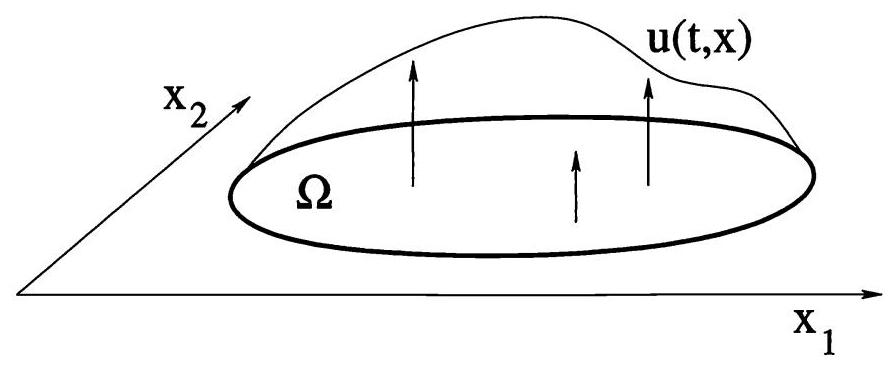
\includegraphics[width=0.8\textwidth]{images/bo_d6ik6nn7aajc739ct1l0_221_293_235_892_366_0.jpg}
\caption{一张弹性膜，沿区域$\Omega$的边界被夹紧，其各点在竖直方向振动.}
\label{fig:linpde-9-3-1}
\end{figure}


\begin{instance}\label{ins:linpde-9-24}
设 $\Omega  \doteq  ( 0,\pi )  \subset  \mathbb{R}$ 与 ${Lu} =  - {u}_{xx}$ .给定 $f \in  {H}_{0}^{1}\left( \Omega \right)$ 与 $g \in  {L}^{2}\left( {( 0,\pi ) }\right)$ ，考虑双曲型初边值问题
\[
\begin{cases} {u}_{tt}  = {u}_{xx}, & t > 0,0 < x < \pi , \\  u\left( {0,x}\right) = f\left( x\right) ,{u}_{t}\left( {0,x}\right)  = g\left( x\right) , & 0 < x < \pi , \\  u\left( {t,0}\right) = u\left( {t,\pi }\right)  = 0. & \end{cases}
\]

在此特殊情形下，公式\eqref{eq:linpde-9-77}以傅里叶正弦级数形式给出解:
{\begin{align}
    u\left( {t,x}\right)  &= \sum_{{k = 1}}^{\infty }\frac{2}{\pi }\left(  {\cos {kt}\left( {{\int }_{0}^{\pi }f\left( y\right) \sin {kydy}}\right) }\right.\\
    &\left. {+\frac{\sin {kt}}{k}\left( {{\int }_{0}^{\pi }g\left( y\right) \sin {kydy}}\right) }\right)  \sin {kx}
\end{align}}
\end{instance}

\section{习题}

\begin{rbhw}[index=1]
设 $\Omega  \doteq  \left\{  {\left( {x,y}\right) ;{x}^{2} + {y}^{2} < 1}\right\}$ 为 ${\mathbb{R}}^{2}$ 中的开单位圆盘.证明:对任意有界可测函数 $f = f\left( {x,y}\right)$ ，问题
\[
\begin{cases}{u}_{xx} + x{u}_{xy} + {u}_{yy} = f,& (x,y)\in \Omega , \\  u = 0, & (x,y)\in \partial \Omega  \end{cases}
\]

存在唯一的弱解.
\end{rbhw}

\begin{rbhw}
设 $\Omega  \doteq  \left\{  {\left( {x,y}\right) ;{x}^{2} + {y}^{2} < 1}\right\}$ 为 ${\mathbb{R}}^{2}$ 中的单位圆盘.在空间 $X = {H}_{0}^{1}\left( \Omega \right)$ 上，考虑内积
\[
\langle u,v{\rangle }_{\diamond } = {\int }_{\Omega }\left(  {{u}_{x}{v}_{x} + 2{u}_{y}{v}_{y} + y\left( {{u}_{x}{v}_{y} + {u}_{y}{v}_{x}}\right) }\right)  {\d xdy}.
\]
\begin{enumerate}[(i)]
    \item 证明 $\langle  \cdot  , \cdot  {\rangle }_{\diamond }$ 确实是 $X$ 上的内积，且使 $X$ 成为Hilbert空间.
    \item 给定 $f \in  {L}^{2}\left( \Omega \right)$ ，证明存在唯一的 $u \in  X$ ，使得
\[
\langle u,v{\rangle }_{\diamond } = {\int }_{\Omega }{fv\d x}\;\forall\,v \in  X = {H}_{0}^{1}\left( \Omega \right) .
\]
$u$ 满足哪个椭圆型方程？
\end{enumerate}
\end{rbhw}

\begin{rbhw}
考虑定义在 ${\mathbb{R}}^{2}$ 上的微分算子
\[
{Lu} =  - {\left( x{u}_{x}\right) }_{x} - {\left( y{u}_{y}\right) }_{y} + 2{u}_{xy} + 3\left( {{u}_{x} + {u}_{y}}\right)  - {6u}.
\]

确定:对哪些有界开集 $\Omega  \subset  {\mathbb{R}}^{2}$ ，算子 $L$ 在 $\Omega$ 上是一致椭圆的.
\end{rbhw}

\begin{rbhw}
设 $\Omega  \subset  {\mathbb{R}}^{n}$ 为有界开集.令 $\beta  > 0$ 为Poincaré不等式中的最佳常数，即
\[
\beta  \doteq  \sup \left\{  {\| u{\| }_{{L}^{2}\left( \Omega \right) };u \in  {H}_{0}^{1}\left( \Omega \right) ,\| \nabla u{\| }_{{L}^{2}\left( \Omega \right) } \leq  1}\right\}  .
\]
\begin{enumerate}[(i)]
    \item 建立算子 ${Lu} =  - {\Delta u}$ 的特征值的下界.更准确地说，若 $\phi  \in  {H}_{0}^{1}\left( \Omega \right)$ 为
\[
\left\{  \begin{aligned}  - {\Delta \phi } &  = {\mu \phi }, & & x \in  \Omega , \\  \phi &  = 0, & & x \in  \partial \Omega , \end{aligned}\right.
\]
提供非平凡弱解，则证明 $\mu  \geq  1/{\beta }^{2}$ .
    \item 证明抛物型初边值问题
\[
\left\{  \begin{aligned} {u}_{t} &  = {\Delta u}, & & t > 0,x \in  \Omega , \\  u\left( {t,x}\right) &  = 0, & & t > 0,x \in  \partial \Omega , \\  u\left( {0,x}\right) &  = g\left( x\right) , & & x \in  \Omega , \end{aligned}\right.
\]
的解当 $t \rightarrow  \infty$ 时衰减至零.事实上，对每个 $t \geq  0$ ，均有 $\| u\left( t\right) {\| }_{{L}^{2}} \leq  {e}^{-t/{\beta }^{2}}\| g{\| }_{{L}^{2}}$.
\end{enumerate}
\end{rbhw}

\begin{rbhw}
设 $\Omega  \subseteq  \widetilde{\Omega } \subset  {\mathbb{R}}^{n}$ 为有界开集.令 $0 < {\mu }_{1} \leq  {\mu }_{2} \leq  \cdots$ 为算子 $- \Delta$ 在 ${H}_{0}^{1}\Omega$ 上的特征值， $0 < {\widetilde{\mu }}_{1} \leq  {\widetilde{\mu }}_{2} \leq  \cdots$ 为算子 $- \Delta$ 在 ${H}_{0}^{1}\left( \widetilde{\Omega }\right)$ 上的特征值.证明 ${\widetilde{\mu }}_{1} \leq  {\mu }_{1}$ .
\end{rbhw}

\begin{rbhw}
在区间 $\left(  {0,T}\right)$ 上，考虑斯特姆-刘维尔特征值问题
\begin{equation}\tag{9.85}\label{eq:linpde-9-85}
\begin{cases} {\left( p\left( t\right) {u}^{\prime }\right) }^{\prime } + q\left( t\right) u &  = {\mu u},\;0 < t < T, \\  u\left( 0\right)  = u\left( T\right) &  = 0. \end{cases}
\end{equation}

假设
\[
p \in  {\mathcal{C}}^{1}\left( {( 0,T) }\right) ,\;q \in  {\mathcal{C}}^{0}\left( \left(  {0,T}\right)  \right) ,\;p\left( t\right)  \geq  \theta  > 0\;\forall\,t.
\]

证明空间 ${L}^{2}\left( \left(  {0,T}\right)  \right)$ 存在一组标准正交基 $\left\{  {{\phi }_{k};k \geq  1}\right\}$ ，其中每个 ${\phi }_{k}$ 均满足\eqref{eq:linpde-9-85}，对应某个适当的特征值 ${\mu }_{k}$ .此外，当 $k \rightarrow  \infty$ 时， ${\mu }_{k} \rightarrow   - \infty$ .

\end{rbhw}

\begin{rbhw}
在定理\ref{thm:linpde-9-9}中，取 ${Lu} =  - {\Delta u}$ .设 $\left\{  {{\phi }_{k};k \geq  1}\right\}$ 是 ${L}^{2}\left( \Omega \right)$ 的一组由 ${L}^{-1}$ 的特征函数构成的标准正交基.证明在此特殊情形下，特征函数 ${\phi }_{k}$ 关于 ${H}^{1}$ 中的内积也两两正交，即当 $j \neq  k$ 时，有 ${\left( {\phi }_{j},{\phi }_{k}\right) }_{{H}^{1}} = 0$ .

\end{rbhw}

\begin{rbhw}
考虑开矩形 $Q \doteq  \{ \left( {x,y}\right) ;0 < x < a,0 < y < b\}$ .定义函数
\[
{\phi }_{m,n}\left( {x,y}\right)  \doteq  \sqrt{\frac{2}{ab}}\sin \frac{m\pi x}{a}\sin \frac{n\pi y}{b},\;m,n \geq  1.
\]
\begin{enumerate}[(i)]
    \item 验证 ${\phi }_{m,n} \in  {H}_{0}^{1}\left( Q\right)$ .此外，证明可数函数集 $\left\{  {{\phi }_{m,n};m,n \geq  1}\right\}$ 构成 ${L}^{2}\left( Q\right)$ 的一组标准正交基，且均由椭圆算子 ${Lu} =  - {\Delta u}$ 的特征函数组成.计算相应的特征值 ${\mu }_{m,n}$ .
    \item 若 $\Omega  \subset  {\mathbb{R}}^{2}$ 是包含于边长为 $a,b$ 的矩形 $Q$ 内部的开区域，则证明
\[
\| u{\| }_{{L}^{2}\left( \Omega \right) } \leq  \frac{ab}{\pi \sqrt{{a}^{2} + {b}^{2}}}\| \nabla u{\| }_{{L}^{2}\left( \Omega \right) }\;\forall\,u \in  {H}_{0}^{1}\left( \Omega \right) .
\]
\end{enumerate}
\end{rbhw}

\begin{rbhw}
在定理\ref{thm:linpde-9-16}的设定下，假设对每个 $f \in  {L}^{2}\left( \Omega \right)$ ，椭圆边值问题\eqref{eq:linpde-9-2}存在唯一解.证明解映射 $f \mapsto  u$ 是从 ${L}^{2}\left( \Omega \right)$ 到其自身的紧算子.

\end{rbhw}

\begin{rbhw}
(Galerkin逼近)设 $\Omega  \subset  {\mathbb{R}}^{n}$ 为有界开集.设 $\left\{  {{\varphi }_{k};k \geq  1}\right\}  ,{\varphi }_{k} \in  {H}_{0}^{1}\left( \Omega \right)$ 是 ${L}^{2}\left( \Omega \right)$ 的一组由拉普拉斯算子 $\Delta$ 的特征函数构成的标准正交基.

设\eqref{eq:linpde-9-1}中的算子 $L$ 一致椭圆，并假设\eqref{eq:linpde-9-11}中对应的双线性型 $B\left(  {\cdot , \cdot  }\right)$ 严格正定.
对给定的 $f \in  {L}^{2}\left( \Omega \right)$ ，按如下方式构造边值问题\eqref{eq:linpde-9-2}的一列近似解 ${u}_{m}$ .
\begin{enumerate}[(i)]
    \item 对固定的 $m \geq  1$ ，定义
\begin{equation}\tag{9.86}\label{eq:linpde-9-86}
{u}_{m}\left( x\right)  = \sum_{{k = 1}}^{m}{\mathrm{c}}_{k}{\varphi }_{k}\left( x\right)
\end{equation}

选取系数 ${\mathrm{c}}_{1},\ldots ,{\mathrm{c}}_{m}$ ，使得
\begin{equation}\tag{9.87}\label{eq:linpde-9-87}
B\left(  {{u}_{m},{\varphi }_{j}}\right)   = {\left( f,{\varphi }_{j}\right) }_{{L}^{2}},\;j = 1,\ldots ,m.
\end{equation}

证明\eqref{eq:linpde-9-87}给出关于 $m$ 个变量 ${\mathrm{c}}_{1},\ldots ,{\mathrm{c}}_{m}$ 的 $m$ 个线性代数方程组成的方程组.证明该方程组存在唯一解.
    \item 令 $m \rightarrow  \infty$ ，证明序列 ${u}_{m}$ 在 ${H}_{0}^{1}\left( \Omega \right)$ 中一致有界，故存在弱收敛子列，记为 ${u}_{{m}_{j}} \rightharpoonup  u$ .证明 $u$ 是方程\eqref{eq:linpde-9-2}的弱解.由唯一性可知，整个序列收敛:当 $m \rightarrow  \infty$ 时， ${u}_{m} \rightharpoonup  u$ .
\end{enumerate}

\end{rbhw}

\begin{rbhw}
在开区间 $\Omega  = ( 0,3)$ 上，考虑边值问题
\begin{equation}\tag{9.88}\label{eq:linpde-9-88}
\begin{cases}  - {u}_{xx} &  = 1,\;0 < x < 3, \\  u\left( 0\right) &  = u\left( 3\right)  = 0. \end{cases}
\end{equation}

考虑两个线性无关函数 ${\varphi }_{1},{\varphi }_{2} \in  {H}_{0}^{1}\left( {( 0,3) }\right)$ ，其定义为
\[
{\varphi }_{1}\left( x\right)  = \begin{cases} x, &x \in  \left(  {0,1}\right)  , \\  2 - x, &x \in  \left(  {1,2}\right)  , \\  0, &x \in  \left(  {2,3}\right)  , \end{cases} \quad {\varphi }_{2}\left( x\right)  = \begin{cases} 0, &x \in  \left(  {0,1}\right)  , \\  x - 1, &x \in  \left(  {1,2}\right)  , \\  3 - x, &x \in  \left(  {2,3}\right)  . \end{cases}
\]

显式计算满足如下条件的Galerkin逼近 $U\left( x\right)  = {\mathrm{c}}_{1}{\varphi }_{1}\left( x\right)  + {\mathrm{c}}_{2}{\varphi }_{2}\left( x\right)$ :
\[
B\left(  {U,{\varphi }_{i}}\right)   = {\int }_{0}^{3}{U}_{x} \cdot  {\varphi }_{i,x}{\d x} = {\int }_{0}^{3}1 \cdot  {\varphi }_{i}{\d x} = {\left( 1,{\varphi }_{i}\right) }_{{L}^{2}},\;i = 1,2.
\]

将 $U$ 与方程\eqref{eq:linpde-9-88}的精确解进行比较.

\end{rbhw}

\begin{rbhw}
设 $\Omega  = \left\{  {\left( {x,y}\right) ;{x}^{2} + {y}^{2} < 1}\right\}$ 为 ${\mathbb{R}}^{2}$ 中的单位开圆盘，且设 $u$ 是如下方程的光滑解:
\begin{equation}\tag{9.89}\label{eq:linpde-9-89}
    \begin{gathered}
        {u}_{tt} = 2{u}_{xx} + y{u}_{xy} + 3{u}_{yy} + \frac{1}{2}{u}_{x},\;(x,y,t)\in\Omega  \times  \left(  {0,T}\right) \\
        u = 0,\;(x,y,t)\in\partial \Omega  \times  \left(  {0,T}\right).
    \end{gathered}
\end{equation}
\begin{enumerate}[(i)]
    \item 将方程\eqref{eq:linpde-9-89}写成形式 ${u}_{tt} + {Lu} = 0$ ，并证明算子 $L$ 在区域 $\Omega$ 上是一致椭圆的.
    \item 定义适当的能量 $e\left( t\right)  =$ [动能] + [弹性势能]，并验证其关于时间恒定.
\end{enumerate}
\end{rbhw}

\begin{rbhw}
考虑\eqref{eq:linpde-9-20}中的齐次线性椭圆算子 $L$ ，假设\eqref{eq:linpde-9-4}成立，且满足 ${a}^{ij} = {a}^{ji} \in  {L}^{\infty }\left( \Omega \right)$ .将引理\ref{lem:linpde-9-7}中的论证加以推广，给出定理\ref{thm:linpde-9-8}的如下替代证明.
\begin{enumerate}[(i)]
    \item 证明\eqref{eq:linpde-9-22}中的双线性泛函 $B$ 是 ${H}_{0}^{1}\left( \Omega \right)$ 上的一个内积.相应的范数
\[
\| u{\| }_{\diamond } \doteq  {\left( \sum_{{i,j = 1}}^{n}{a}^{ij}\left( x\right) {u}_{{x}_{i}}{u}_{{x}_{j}}\right) }^{1/2}
\]
等价于 ${H}^{1}$ 范数，即
\[
\frac{1}{C} \cdot  \| u{\| }_{{H}^{1}} \leq  \| u{\| }_{\diamond } \leq  C\| u{\| }_{{H}^{1}}\;\forall\,u \in  {H}_{0}^{1}\left( \Omega \right) .
\]
    \item 记 ${H}_{\diamond }$ 为赋予该等价范数的Hilbert空间 ${H}_{0}^{1}$ .仿照引理\ref{lem:linpde-9-7}的证明，利用下图构造\eqref{eq:linpde-9-19}的解 $u = {\iota }^{ * }f$ :
    \begin{gather*}
        {H}_{\diamond }\left( \Omega \right) \overset{\iota }{ \rightarrow  }{L}^{2}\left( \Omega \right)\\
        {H}_{\diamond }\left( \Omega \right)  = {\left(  {H}_{\diamond }\left( \Omega \right) \right)  }^{ * }\overset{{\iota }^{ * }}{ \leftarrow  }{\left(  {L}^{2}\left( \Omega \right) \right)  }^{ * } = {L}^{2}\left( \Omega \right) .
    \end{gather*}
其中 $\iota$ 是 ${H}_{\diamond }$ 到 ${L}^{2}$ 的典范嵌入，而 ${\iota }^{ * }$ 是其伴随算子.
\end{enumerate}
\end{rbhw}

\begin{rbhw}
设 $\Omega  \subset  {\mathbb{R}}^{N}$ 是一个有界开集.在引理\ref{lem:linpde-9-19}的同一设定下，证明映射 $t \mapsto  u\left( t\right)$从$(0,T)$ 到 ${L}^{2}\left( \Omega \right)$是${\mathcal{C}}^{\infty }$的.
\end{rbhw}

\begin{rbhw}
(Neumann问题)设 $\Omega$ 是一个具有光滑边界 $\partial \Omega$ 的有界连通开集.依定义，函数 $u \in  {H}^{1}\left( \Omega \right)$ 是Neumann问题\footnote{此处及后续， $\frac{\partial u}{\partial \nu }$ 表示 $u$ 沿 $\Omega$ 边界外法向的方向导数.}的弱解:
\begin{equation}\tag{9.90}\label{eq:linpde-9-90}
\begin{cases}  - {\Delta u}  = f, & x \in  \Omega , \\  \frac{\partial u}{\partial \nu }  = 0, & x \in  \partial \Omega , \end{cases}
\end{equation}
若
\begin{equation}\tag{9.91}\label{eq:linpde-9-91}
{\int }_{\Omega }\nabla u \cdot  \nabla {v\d x} = {\int }_{\Omega }{fv\d x}\;\forall\,v \in  {H}^{1}\left( \Omega \right) .
\end{equation}

给定 $f \in  {L}^{2}\left( \Omega \right)$ ，证明诺伊曼问题\eqref{eq:linpde-9-90}存在弱解当且仅当
\[
{\int }_{\Omega }{f\d x} = 0.
\]
{\textcolor{gray}{提示:首先证明，对 $\gamma  > 0$ ，双线性型
\[
{B}_{\gamma }\left(  {u,v}\right)   \doteq  {\int }_{\Omega }\left( {\nabla u \cdot  \nabla v + {\gamma uv}}\right) {\d x}
\]
在 ${H}^{1}\left( \Omega \right)$ 上严格正定.将\eqref{eq:linpde-9-90}的弱解用逆算子 ${L}_{\gamma }^{-1}$ 表示，其中 ${L}_{\gamma }u =  - {\Delta u} + {\gamma u}$ .}}


\end{rbhw}

\begin{rbhw}
(双调和方程)设 $\Omega  \subset  {\mathbb{R}}^{n}$ 为具有光滑边界的有界开集.函数 $u \in  {H}_{0}^{2}\left( \Omega \right)$ 是双调和方程的弱解，若
\begin{equation}\tag{9.92}\label{eq:linpde-9-92}
\begin{cases} {\Delta }^{2}u = f, & x \in  \Omega , \\  u = \frac{\partial u}{\partial \nu } = 0, & x \in  \partial \Omega , \end{cases}
\end{equation}

若
\begin{equation}\tag{9.93}\label{eq:linpde-9-93}
{\int }_{\Omega }{\Delta u\Delta v\d x} = {\int }_{\Omega }{fv\d x}\;\forall\,v \in  {H}_{0}^{2}\left( \Omega \right) .
\end{equation}
给定 $f \in  {L}^{2}\left( \Omega \right)$ ，证明边值问题\eqref{eq:linpde-9-92}存在唯一弱解.

{\textcolor{gray}{提示:证明由\eqref{eq:linpde-9-93}左端定义的、定义在 ${H}_{0}^{2}\left( \Omega \right)$ 上的双线性型 $B\left(  {u,v}\right)$ 在 ${H}_{0}^{2}\left( \Omega \right)$ 上严格正定.}}

\end{rbhw}

\appendix
\chapter{背景知识}

\section{偏序集}

集合 $S$ 若配备二元关系 $\preccurlyeq$ 而成为偏序集，则对任意 $a,b,c \in  S$ ，均有

(i) $a \preccurlyeq  a$ ,

(ii) $a \preccurlyeq  b$ 且 $b \preccurlyeq  a$ 蕴含 $a = b$ ，

(iii) $a \preccurlyeq  b$ 且 $b \preccurlyeq  c$ 蕴含 $a \preccurlyeq  c$ .

偏序集 $S$ 的子集 ${S}^{\prime } \subseteq  S$ 称为全序的，若对任意 $a,b \in  {S}^{\prime }$ ，总有 $a \preccurlyeq  b$ 或 $b \preccurlyeq  a$ 成立.若 ${S}^{\prime }$ 不被任何其他全序集真包含，则称该子集 ${S}^{\prime }$ 为极大(关于全序性而言).

利用Zorn引理或选择公理，可证得

\begin{theorem}[Hausdorff极大性原理]\label{thm:app-A-1}
若 $S$ 为任意偏序集，则其任一全序子集 ${S}^{\prime } \subseteq  S$ 均包含于某个极大全序子集中.
\end{theorem}

\section{度量空间与拓扑空间}

集合 $X$ 上的距离是指满足以下三条性质的映射 $d : X \times  X \mapsto  {\mathbb{R}}_{ + }$ :

(1) 正定性: $d\left( {x,y}\right)  \geq  0,d\left( {x,y}\right)  = 0$ 当且仅当 $x = y$ ，

(2) 对称性: $d\left( {x,y}\right)  = d\left( {y,x}\right)$ ，

(3) 三角不等式: $d\left( {x,z}\right)  \leq  d\left( {x,y}\right)  + d\left( {y,z}\right)$ .

配备距离函数 $d\left( {\cdot , \cdot  }\right)$ 的集合 $X$ 称为度量空间.

以点 $x$ 为中心、半径为 $r > 0$ 的开球是如下集合

\[
B\left( {x,r}\right)  \doteq  \{ y \in  X;d\left( {y,x}\right)  < r\} .
\]

反过来，度量 $d\left( {\cdot , \cdot  }\right)$ 在 $X$ 上确定一个拓扑.

子集 $A \subseteq  X$ 是开集，若对每个 $x \in  A$ ，均存在半径 $r > 0$ ，使得 $B\left( {x,r}\right)  \subseteq  A$ .

子集 $C \subseteq  X$ 是闭集，若其补集 $X \setminus  C = \{ x \in  X;x \notin  C\}$ 是开集.

若 $B\left( {x,r}\right)  \subseteq  A$ 对某个 $r > 0$ 成立，则称 $A$ 是点 $x$ 的邻域，或等价地称 $x$ 是 $A$ 的内点.

— 任意一族开集的并集是开集；有限个开集的交集是开集.

— 任意一族闭集的交集是闭集；有限个闭集的并集是闭集.

全空间 $X$ 和空集 $\varnothing$ 恒既开又闭.若不存在其他同时既开又闭的子集 $S \subset  X$ ，则称空间 $X$ 是连通的.

序列 ${\left( {x}_{n}\right) }_{n \geq  1}$ 收敛于点 $x \in  X$ ，若
\[
\mathop{\lim }\limits_{{n \rightarrow  \infty }}d\left( {{x}_{n},x}\right)  = 0.
\]

此时记作 $\mathop{\lim }\limits_{{n \rightarrow  \infty }}{x}_{n} = x$ ，或简记为 ${x}_{n} \rightarrow  x$ .

集合 $A$ 的闭包记为 $\bar{A}$ ，是包含 $A$ 的最小闭集；它由所有包含 $A$ 的闭集之交给出.点 $x$ 属于集合 $A$ 的闭包，当且仅当存在一列点 ${x}_{n} \in  A$ 收敛于 $x$ .

子集 $S \subseteq  X$ 在 $X$ 中稠密，若 $\bar{S} = X$ .这等价于: $S$ 与 $X$ 的每个非空开子集均相交.若空间 $X$ 含有可数稠密子集，则称其为可分的.

序列 ${\left( {x}_{n}\right) }_{n \geq  1}$ 是Cauchy序列，如果对任意 $\varepsilon  > 0$ ，存在足够大的整数 $N$ ，使得
\[
d\left( {{x}_{m},{x}_{n}}\right)  \leq  \varepsilon \;\text{当}\; m,n \geq  N.
\]

度量空间 $X$ 是完备的，如果每个Cauchy序列都收敛于某个极限点 $x \in  X$ .

若 $X,Y$ 是两个度量空间，则映射 $f : X \mapsto  Y$ 连续，当且仅当对每个开集 $A \subseteq  Y$，其原像 ${f}^{-1}\left( A\right)  \doteq  \{ x \in  X;f\left( x\right)  \in  A\}$ 是 $X$ 中的开子集.

映射 $f : X \mapsto  Y$ 连续当且仅当，对每个 ${x}_{0} \in  X$ 和 $\varepsilon  > 0$ ，存在 $\delta  > 0$ ，使得
\[
d\left( {x,{x}_{0}}\right)  < \delta \;\implies \;d\left( {f\left( x\right) ,f\left( {x}_{0}\right) }\right)  < \varepsilon .
\]

我们称函数 $f : X \mapsto  Y$ 是Lipschitz连续的，如果存在常数 $C \geq  0$ ，使得
\[
d\left( {f\left( x\right) ,f\left( {x}^{\prime }\right) }\right)  \leq  C \cdot  d\left( {x,{x}^{\prime }}\right) \;\forall\,x,{x}^{\prime } \in  X.
\]

更一般地，我们称 $f : X \mapsto  Y$ 是指数为 $0 < \alpha  \leq  1$ 的Hölder连续函数，如果存在常数 $C$ ，使得
\[
d\left( {f\left( x\right) ,f\left( {x}^{\prime }\right) }\right)  \leq  C \cdot  {\left(  d\left( x,{x}^{\prime }\right) \right)  }^{\alpha }\;\forall\,x,{x}^{\prime } \in  X.
\]

一族满足 $K \subseteq  \mathop{\bigcup }\limits_{{i \in  \mathcal{I}}}{A}_{i}$ 的开集 $\left\{  {{A}_{i};i \in  \mathcal{I}}\right\}$ 称为集合 $K$ 的一个开覆盖.此处指标集 $\mathcal{I}$ 可以是无限的.集合 $K \subseteq  X$ 是紧的，如果对 $K$ 的任意开覆盖，均可提取出一个有限子覆盖.

集合 $S$ 是相对紧的，如果其闭包 $\bar{S}$ 是紧的.

集合 $S$ 是预紧的，如果对任意 $\varepsilon  > 0$ ，它可被有限个半径为 $\varepsilon$ 的球所覆盖.

\begin{theorem}[${\mathbb{R}}^{n}$ 中的紧子集]\label{thm:app-A-2}
子集 $S \subset  {\mathbb{R}}^{n}$ 是紧的当且仅当它既闭又有界.
\end{theorem}

\begin{theorem}[紧性的等价刻画]\label{thm:app-A-3}
设 $S$ 是一个度量空间.以下命题等价:

(i) $S$ 是紧的.

(ii) $S$ 是预紧的且完备的.

(iii) 对 $S$ 中任意点列 ${\left( {x}_{k}\right) }_{k \geq  1}$ ，均可提取出一个收敛于某极限点 $x \in  S$ 的子列.
\end{theorem}

\subsection{压缩映射的不动点}
设 $\phi  : X \mapsto  X$是从完备度量空间 $X$ 到其自身的映射.满足$\phi \left( {x}^{ * }\right)  = {x}^{ * }$ 的点 ${x}^{ * }$ 称为 $\phi$ 的不动点.对严格压缩映射，该不动点唯一，且可通过简单的迭代程序得到.

\begin{theorem}[压缩映射定理]\label{thm:app-A-4}
设 $X$ 是一个完备度量空间， $\phi  : X \mapsto  X$ 是一个连续映射，且对某个 $\kappa  < 1$ ，有
\begin{equation}\tag{A.1}\label{eq:app-A-1}
d\left( {\phi \left( x\right) ,\phi \left( y\right) }\right)  \leq  {\kappa d}\left( {x,y}\right) \;\forall\,x,y \in  X.
\end{equation}

此时存在唯一一点 ${x}^{ * } \in  X$ ，使得
\begin{equation}\tag{A.2}\label{eq:app-A-2}
{x}^{ * } = \phi \left( {x}^{ * }\right) .
\end{equation}

此外，对任意 $y \in  X$ ，均有
\begin{equation}\tag{A.3}\label{eq:app-A-3}
d\left( {y,{x}^{ * }}\right)  \leq  \frac{1}{1 - \kappa }d\left( {y,\phi \left( y\right) }\right) .
\end{equation}
\end{theorem}

\begin{proof}
任取一点 $y \in  X$ ，并考虑序列
\[
{y}_{0} = y,\;{y}_{1} = \phi \left( {y}_{0}\right) ,\;\ldots ,\;{y}_{n + 1} = \phi \left( {y}_{n}\right) ,\;\ldots
\]

由归纳法可得
{\setjot[-2]\begin{gather*}
    d\left( {{y}_{2},{y}_{1}}\right)  \leq  {\kappa d}\left( {{y}_{1},{y}_{0}}\right)\\
    d\left( {{y}_{3},{y}_{2}}\right)  \leq  {\kappa d}\left( {{y}_{2},{y}_{1}}\right)  \leq  {\kappa }^{2}d\left( {{y}_{1},{y}_{0}}\right)\\
    \cdots \\
d\left( {{y}_{n + 1},{y}_{n}}\right)  \leq  {\kappa d}\left( {{y}_{n},{y}_{n - 1}}\right)  \leq  {\kappa }^{n}d\left( {{y}_{1},{y}_{0}}\right)  = {\kappa }^{n}d\left( {\phi \left( y\right) ,y}\right) .
\end{gather*}}

在$m < n$ 处有
\begin{equation}\tag{A.4}\label{eq:app-A-4}
d\left( {{y}_{n},{y}_{m}}\right)  \leq  \sum_{{j = m}}^{{n - 1}}d\left( {{y}_{j + 1},{y}_{j}}\right)  \leq  \sum_{{j = m}}^{{n - 1}}{\kappa }^{j}d\left( {y,\phi \left( y\right) }\right)  \leq  \frac{{\kappa }^{m}}{1 - \kappa }d\left( {y,\phi \left( y\right) }\right) .
\end{equation}

由于 $\kappa  < 1$ ，\eqref{eq:app-A-4}式右端当 $m \rightarrow  \infty$ 时趋于零，故序列 ${\left( {y}_{n}\right) }_{n \geq  1}$ 为Cauchy列.又因 $X$ 完备，该序列收敛于某极限点 ${x}^{ * }$ .由 $\phi$ 的连续性可得
\[
{x}^{ * } = \mathop{\lim }\limits_{{n \rightarrow  \infty }}{y}_{n} = \mathop{\lim }\limits_{{n \rightarrow  \infty }}\phi \left( {y}_{n - 1}\right)  = \phi \left( {\mathop{\lim }\limits_{{n \rightarrow  \infty }}{y}_{n - 1}}\right)  = \phi \left( {x}^{ * }\right)
\]

因而\eqref{eq:app-A-2}成立.不动点 ${x}^{ * }$ 的唯一性证明如下:若
\[
{x}_{1} = \phi \left( {x}_{1}\right) ,\;{x}_{2} = \phi \left( {x}_{2}\right) ,
\]

则由\eqref{eq:app-A-1}可得
\[
d\left( {{x}_{1},{x}_{2}}\right)  = d\left( {\phi \left( {x}_{1}\right) ,\phi \left( {x}_{2}\right) }\right)  \leq  {\kappa d}\left( {{x}_{1},{x}_{2}}\right) .
\]

$\kappa  < 1$ 的假设从而推出 $d\left( {{x}_{1},{x}_{2}}\right)  = 0$ ，进而推出 ${x}_{1} = {x}_{2}$ .

最后，在\eqref{eq:app-A-4}中取 $m = 0$ ，对任意 $n \geq  1$ 可得
\[
d\left( {{y}_{n},y}\right)  \leq  \frac{1}{1 - \kappa }d\left( {y,\phi \left( y\right) }\right) .
\]

令 $n \rightarrow  \infty$ ，即得\eqref{eq:app-A-3}.
\end{proof}

\subsection{Baire纲定理}设 $X$ 为度量空间.在 $X$ 的所有子集中，我们希望定义一族“大集”与一族“小集”，使其满足如下自然性质:

(i) 集合 $S \subseteq  X$ 为大集当且仅当其补集 $X \setminus  S$ 为小集.

(ii) 可数个大集的交集仍为大集.

(iii) 大集非空.

若给定 $\mu$ 在 $X$ 上的概率测度，则可将概率为一的集合称为“大集合”，将概率为零的集合称为“小集合”.按此定义，所有性质 (i)-(iii) 显然成立.

若度量空间 $X$ 完备，则可借助Baire纲理论，仅依据其拓扑结构引入“大集”与“小集”的概念.具体而言，称集合 $S \subseteq  X$ 为第二纲集(即“拓扑意义下大集”)，若 $S$ 是可数个开稠密集的交集；而称集合 $S \subseteq  X$ 为第一纲集(即等价地称为“贫集”，亦即“拓扑意义下小集”)，若 $S$ 是可数个无内点闭集的并集.由定义可知，此类拓扑意义下的大集或小集显然满足上述性质(i)与(ii).性质(iii)亦成立，则是如下定理的重要推论.

\begin{theorem}[Baire]\label{thm:app-A-5}
设 ${\left( {V}_{k}\right) }_{k \geq  1}$ 为完备度量空间 $X$ 中一列开稠密子集，则其交集 $V \doteq  \mathop{\bigcap }\limits_{{k = 1}}^{\infty }{V}_{k}$ 是 $X$ 中一个非空稠密子集.
\end{theorem}

\begin{proof}
设 $\Omega  \subset  X$ 为任意开集，需证 $\left( {\mathop{\bigcap }\limits_{{k = 1}}^{\infty }{V}_{k}}\right)  \cap  \Omega$ 非空.

选取一点 ${x}_{0}$ 及半径 ${r}_{0} < 1$ ，使得 $B\left( {{x}_{0},3{r}_{0}}\right)  \subset  \Omega$ .

由归纳法，对每个 $k \geq  1$ ，我们选取一点 ${x}_{k}$ 和半径 ${r}_{k}$ ，使得 $B\left( {{x}_{k},3{r}_{k}}\right)  \subset  {V}_{k} \cap  B\left( {{x}_{k - 1},{r}_{k - 1}}\right)$ .这可行，因为 ${V}_{k}$ 既开又稠密.对每个 $k \geq  1$ ，上述选取意味着
\[
{r}_{k + 1} \leq  \frac{{r}_{k}}{3},\;d\left( {{x}_{k + 1},{x}_{k}}\right)  \leq  {r}_{k} \leq  \frac{1}{{3}^{k}}.
\]

因此，序列 ${\left( {x}_{k}\right) }_{k \geq  1}$ 是Cauchy列.由于 $X$ 完备，该序列收敛:存在某 ${x}^{ * } \in  X$ ，使得 ${x}_{k} \rightarrow  {x}^{ * }$ .
\[
d\left( {{x}^{ * },{x}_{k}}\right)  \leq  \sum_{{j = k}}^{\infty }d\left( {{x}_{j + 1},{x}_{j}}\right)  \leq  \sum_{{j = k}}^{\infty }{r}_{j} \leq  \sum_{{j = k}}^{\infty }{3}^{k - j}{r}_{k} = \frac{3}{2}{r}_{k}.
\]

故对每个 $k \geq  1$ ，有
\[
{x}^{ * } \in  B\left( {{x}_{k},3{r}_{k}}\right)  \subset  {V}_{k}.
\]

当 $k = 0$ 时，同一论证得出 ${x}^{ * } \in  B\left( {{x}_{0},3{r}_{0}}\right)  \subset  \Omega$ .因此 ${x}^{ * } \in  \left( {\mathop{\bigcap }\limits_{{k = 1}}^{\infty }{V}_{k}}\right)  \cap  \Omega$.
\end{proof}

\section{Lebesgue测度理论回顾}

\subsection{可测集}
集合 ${\mathbb{R}}^{n}$ 的子集族 $\mathcal{F}$ 称为 $\sigma$ -代数，若满足

(i) $\varnothing  \in  \mathcal{F}$ 且 ${\mathbb{R}}^{n} \in  \mathcal{F}$ ；

(ii) 若 $A \in  \mathcal{F}$ ，则 ${\mathbb{R}}^{n} \setminus  A \in  \mathcal{F}$ ；

(iii) 若对每个 $k \geq  1$ 均有 ${A}_{k} \in  \mathcal{F}$ ，则 $\mathop{\bigcup }\limits_{{k = 1}}^{\infty }{A}_{k} \in  \mathcal{F}$ 且 $\mathop{\bigcap }\limits_{{k = 1}}^{\infty }{A}_{k} \in  \mathcal{F}$ .

\begin{theorem}[${\mathbb{R}}^{n}$ 上Lebesgue测度的存在性]\label{thm:app-A-6}
存在 ${\mathbb{R}}^{n}$ 的一个 $\sigma$ -代数 $\mathcal{F}$ ，以及一个映射 $A \mapsto  {m}_{n}\left( A\right)$ : $\mathcal{F}$ → $\left(  {0, + \infty }\right)$ ，具有如下性质.
\begin{enumerate}[(i)]
    \item $\mathcal{F}$ 包含 ${\mathbb{R}}^{n}$ 的所有开子集，从而也包含 ${\mathbb{R}}^{n}$ 的所有闭子集.
    \item 若 $B$ 是 ${\mathbb{R}}^{n}$ 中的一个球，则 ${m}_{n}\left( B\right)$ 等于 $B$ 的 $n$ -维体积.
    \item 若对每个 $k \geq  1$ 有 ${A}_{k} \in  \mathcal{F}$ ，且集合 ${A}_{k}$ 两两不交，则
\[
{m}_{n}\left( \mathop{\bigcup }\limits_{{k = 1}}^{\infty }\right)  = \sum_{{k = 1}}^{\infty }{m}_{n}\left( {A}_{k}\right)
\]
    \item 若 $A \subseteq  B$ 与 $B \in  \mathcal{F}$ 和 ${m}_{n}\left( B\right)  = 0$ 成立，则 $A \in  \mathcal{F}$ 与 ${m}_{n}\left( A\right)  = 0.$ 亦成立.
\end{enumerate}
\end{theorem}

包含在 $\sigma$ -代数 $\mathcal{F}$ 中的集合称为Lebesgue可测集，而 ${m}_{n}\left( A\right)$ 是集合 $A \in  \mathcal{F}$ 的 $n$ 维Lebesgue测度.

若性质 $P\left( x\right)$ 对所有点 $x \in  {\mathbb{R}}^{n}$ 均成立，仅在某个可测集 $\mathcal{N}$ (满足 ${m}_{n}\left( \mathcal{N}\right)  = 0$ )上的点除外，则称该性质 $P$ 几乎处处(a.e.)成立.

函数 $f : {\mathbb{R}}^{n} \mapsto  \mathbb{R}$ 可测，当且仅当
\[
{f}^{-1}\left( U\right)  \doteq  \left\{  {x \in  {\mathbb{R}}^{n};f\left( x\right)  \in  U}\right\}   \in  \mathcal{F}
\]

对每个开集 $U \subseteq  \mathbb{R}$ 成立.

每个连续函数均可测.若 $f,g$ 可测，则 $f + g$ 与 $f \cdot  g$ 也可测.对任一一致有界的可测函数列 ${\left( {f}_{k}\right) }_{k \geq  1}$ ，如下定义的函数
\[
{f}^{ * }\left( x\right)  \doteq  \limsup_{{k \rightarrow  \infty }}{f}_{k}\left( x\right) ,\;{f}_{ * }\left( x\right)  \doteq  \mathop{\liminf }\limits_{{k \rightarrow  \infty }}{f}_{k}\left( x\right)
\]

均为可测函数.可测函数 $f$ 的本性上确界定义为
\[
\mathrm{ess}\sup f \doteq  \inf \left\{  {\alpha  \in  \mathbb{R};f\left( x\right)  < \alpha \text{ a.e. }x \in  {\mathbb{R}}^{n}}\right\}  \text{ . }
\]

\begin{theorem}[Egoroff]\label{thm:app-A-7}
设 ${\left( {f}_{k}\right) }_{k \geq  1}$ 为一可测函数列，且点态收敛
\[
{f}_{k}\left( x\right)  \rightarrow  f\left( x\right) \;\text{a.e. }x \in  A,
\]

于某个可测函数 $f$ 及某个满足 ${m}_{n}\left( A\right)  < \; \infty$ 的可测集 $A \subset  {\mathbb{R}}^{n}$ 上.则对每个 $\varepsilon  > 0$ ，存在子集 $E \subseteq  A$ ，使得

(i) ${m}_{n}\left( {A \setminus  E}\right)  \leq  \varepsilon$ ,

(ii) ${f}_{k} \rightarrow  f$ 在 $E$ 上一致收敛.
\end{theorem}

\subsection{Lebesgue积分}
为定义Lebesgue积分，需从一类特殊函数出发.集合 $A$ 的特征函数为
\[
{\chi }_{A}\left( x\right)  = \begin{cases} 1, &x \in  A, \\  0 , &x \notin  A. \end{cases}
\]

仅取有限个值的函数，即形如
\begin{equation}\tag{A.5}\label{eq:app-A-5}
g\left( x\right)  = \sum_{{i = 1}}^{N}{c}_{i}{\chi }_{{A}_{i}}\left( x\right)
\end{equation}
的函数(其中 ${A}_{1},\ldots ,{A}_{N} \subset  {\mathbb{R}}^{n}$ 为互不相交的可测集， ${c}_{1},\ldots ,{c}_{N} \in \; \mathbb{R}$ 为常数)，称为简单函数.若 \eqref{eq:app-A-5} 中的函数 $g$ 非负，则其Lebesgue积分定义为
\[
{\int }_{{\mathbb{R}}^{n}}{g\d x} \doteq  \sum_{{i = 1}}^{N}{\mathrm{c}}_{i}{m}_{n}\left( {A}_{i}\right)
\]

同前， ${m}_{n}\left( {A}_{i}\right)$ 表示集合 ${A}_{i}$ 的 $n$ 维Lebesgue测度.更一般地，若 $f : {\mathbb{R}}^{n} \mapsto  \mathbb{R}$ 为非负可测函数，则其Lebesgue积分定义为
\[
{\int }_{{\mathbb{R}}^{n}}{f\d x} \doteq  \sup \left\{  {{\int }_{{\mathbb{R}}^{n}}{g\d x};g\text{ is simple, }g \leq  f}\right\}  .
\]

对任意可测函数 $f : {\mathbb{R}}^{n} \mapsto  \mathbb{R}$ ，其正部与负部分别记为
\[
{f}_{ + } \doteq  \max \{ f,0\} ,\;{f}_{ - } \doteq  \max \{  - f,0\} .
\]

于是定义 $f$ 的Lebesgue积分为
\begin{equation}\tag{A.6}\label{eq:app-A-6}
{\int }_{{\mathbb{R}}^{n}}{f\d x} \doteq  {\int }_{{\mathbb{R}}^{n}}{f}_{ + }{\d x} - {\int }_{{\mathbb{R}}^{n}}{f}_{ - }{\d x}
\end{equation}
前提是右侧至少有一项为有限值.此时称 $f$ 可积.注意，\eqref{eq:app-A-6}式中的积分可能为 $+ \infty$ 或 $- \infty$ .

若可测函数 $f : {\mathbb{R}}^{n} \mapsto  \mathbb{R}$ 满足
\[
{\int }_{{\mathbb{R}}^{n}}\left| f\right| {\d x} < \infty
\]

若对每个紧集 $K \subset  {\mathbb{R}}^{n}$ ，乘积 $f \cdot  {\chi }_{K}$ 均可求和，则称 $f$ 为局部可求和的.

Lebesgue积分具有良好的收敛性质.

\begin{theorem}[Fatou引理]\label{thm:app-A-8}
设 ${\left( {f}_{k}\right) }_{k \geq  1}$ 为一列非负且可求和的函数，则
\[
{\int }_{{\mathbb{R}}^{n}}\left( {\mathop{\liminf }\limits_{{k \rightarrow  \infty }}{f}_{k}}\right) {\d x} \leq  \mathop{\liminf }\limits_{{k \rightarrow  \infty }}{\int }_{{\mathbb{R}}^{n}}{f}_{k}{\d x}.
\]
\end{theorem}

\begin{theorem}[单调收敛定理]\label{thm:app-A-9}
设 ${\left( {f}_{k}\right) }_{k \geq  1}$ 为一列可测函数，使得 ${f}_{1}$ 可求和且 ${f}_{1} \leq  {f}_{2} \leq  \cdots  \leq  {f}_{k} \leq \; {f}_{k + 1} \leq  \cdots$ ，则
\[
{\int }_{{\mathbb{R}}^{n}}\left( {\mathop{\lim }\limits_{{k \rightarrow  \infty }}{f}_{k}}\right) {\d x} = \mathop{\lim }\limits_{{k \rightarrow  \infty }}{\int }_{{\mathbb{R}}^{n}}{f}_{k}{\d x}.
\]
\end{theorem}

\begin{theorem}[Lebesgue控制收敛定理]\label{thm:app-A-10}
设 ${\left( {f}_{k}\right) }_{k \geq  1}$ 为一列可测函数，满足
\[
{f}_{k}\left( x\right)  \rightarrow  f\left( x\right) \;\text{ a.e. }x \in  {\mathbb{R}}^{n}.
\]

此外，假设存在一个可求和函数 $g$ ，使得
\[
\left| {{f}_{k}\left( x\right) }\right|  \leq  g\left( x\right),\;\forall\,k \geq  1\text{ 且 a.e. }x \in  {\mathbb{R}}^{n}.
\]

则
\[
\mathop{\lim }\limits_{{k \rightarrow  \infty }}{\int }_{{\mathbb{R}}^{n}}{f}_{k}{\d x} = {\int }_{{\mathbb{R}}^{n}}{f\d x}.
\]
\end{theorem}

给定Lebesgue可测集 $U \subset  {\mathbb{R}}^{n}$ ，可测函数 $f : U \mapsto  \mathbb{R}$ 关于Lebesgue测度 $c$ 的积分可定义为
\[
{\int }_{U}{f\d x} \doteq  {\int }_{{\mathbb{R}}^{n}}\widetilde{f}{\d x},\;\text{ 其中 }\;\widetilde{f}\left( x\right)  \doteq  \begin{cases} f\left( x\right), & x\in  U, \\  0, & x \notin  U. \end{cases}
\]

其中 $1 \leq  p < \infty ,{L}^{p}\left( U\right)$ 表示所有Lebesgue可测函数 $f : U \mapsto  \mathbb{R}$ 构成的空间，且满足
\begin{equation}\tag{A.7}\label{eq:app-A-7}
\| f{\| }_{{L}^{p}\left( U\right) } \doteq  {\left( {\int }_{U}{\left| f\right| }^{p}\d x\right) }^{1/p} < \infty .
\end{equation}

此外， ${L}^{\infty }\left( U\right)$ 记为所有本质有界即可测函数 $f : U \mapsto  \mathbb{R}$ 构成的空间，即满足
\begin{equation}\tag{A.8}\label{eq:app-A-8}
\| f{\| }_{{L}^{\infty }\left( U\right) } \doteq  \text{ess}\mathop{\sup}\limits_{{x \in  U}}\left| {f\left( x\right) }\right|  < \infty .
\end{equation}

在零测集之外取值相同的两个函数，被视为 ${L}^{p}$ 或 ${L}^{\infty }$ 中的同一元素.

给定开集 $\Omega  \subseteq  {\mathbb{R}}^{n}$ 及 $1 \leq  p \leq  \infty$ ，用 ${L}_{\text{ loc }}^{p}\left( \Omega \right)$ 表示所有满足如下条件的可测函数 $f : \Omega  \mapsto  \mathbb{R}$ 构成的空间:对每个闭包含于 $\Omega$ 内的有界开集 $U$ ，均有 $f \in  {L}^{p}\left( U\right)$ .若 $0 < {m}_{n}\left( \Omega \right)  < \infty$ ，则 $f$ 在集合 $\Omega$ 上的平均值定义为
\[
{\oint }_{\Omega }{f\d x} \doteq  \frac{1}{{m}_{n}\left( \Omega \right) }{\int }_{\Omega }{f\d x}.
\]

注意到，函数 $f$ 在点 ${x}_{0}$ 处连续当且仅当
\begin{equation}\tag{A.9}\label{eq:app-A-9}
\mathop{\lim }\limits_{{r \rightarrow  0 + }}\mathop{\sup }\limits_{{x \in  B\left( {{x}_{0},r}\right) }}\left| {f\left( x\right)  - f\left( {x}_{0}\right) }\right|  = 0.
\end{equation}

将上确界替换为平均值，称 $f$ 在点 ${x}_{0}$ 处拟连续，若
\begin{equation}\tag{A.10}\label{eq:app-A-10}
\mathop{\lim }\limits_{{r \rightarrow  0 + }}{\oint }_{B\left( {{x}_{0},r}\right) }\left| {f\left( x\right)  - f\left( {x}_{0}\right) }\right| {\d x} = 0.
\end{equation}

\begin{theorem}[Lebesgue]\label{thm:app-A-11}
设 $f : {\mathbb{R}}^{n} \mapsto  \mathbb{R}$ 局部可积，则 $f$ 在几乎处处点 ${x}_{0} \in  {\mathbb{R}}^{n}$ 处拟连续.
\end{theorem}

满足 \eqref{eq:app-A-10} 的点 ${x}_{0}$ 称为 $f$ 的Lebesgue点.

给定区间 $\left(  {a,b}\right)   \subset  \mathbb{R}$ ，函数 $F : \left(  {a,b}\right)   \mapsto  \mathbb{R}$ 绝对连续是指:对任意 $\varepsilon  > 0$ ，存在 $\delta  > 0$ ，使得对任意有限族含于 $\left(  {a,b}\right)$ 的互不相交区间 $\left(  {{a}_{1},{b}_{1}}\right)  ,\ldots ,\left(  {{a}_{n},{b}_{n}}\right)$ ，均有

\[
\sum_{{i = 1}}^{n}\left( {{b}_{i} - {a}_{i}}\right)  < \delta \implies\sum_{{i = 1}}^{n}\left| {F\left( {b}_{i}\right)  - F\left( {a}_{i}\right) }\right|  < \varepsilon .
\]

\begin{theorem}[绝对连续函数]\label{thm:app-A-12}
以下条件等价.

(i) $F : \left(  {a,b}\right)   \mapsto  \mathbb{R}$ 绝对连续.

(ii) 存在函数 $f \in  {L}^{1}\left( \left(  {a,b}\right)  \right)$ ，使得
\[
F\left( x\right)  = F\left( a\right)  + {\int }_{\left(  a,x\right)  }f\left( x\right) {\d x},\;\forall\,x \in  \left(  {a,b}\right)  .
\]

若 (i) 与 (ii) 成立，则 $F$ 几乎处处可微，且其导数为 ${F}^{\prime }\left( x\right)  = f\left( x\right)$ ，对几乎处处的 $x \in  \left(  {a,b}\right)$ 成立.
\end{theorem}

接下来考虑两个可测子集 $X \subseteq  {\mathbb{R}}^{m}$ 和 $Y \subseteq  {\mathbb{R}}^{n}$ ，使得笛卡尔积
\[
X \times  Y \doteq  \{ \left( {x,y}\right) ;x \in  X,y \in  Y\}
\]

是 ${\mathbb{R}}^{m + n}$ 的一个可测子集.对二元函数 $f$ : $X \times  Y \mapsto  \mathbb{R}$ ，对每个固定的 $x$ ，我们考虑仅关于变量 $y$ 的函数 $y \mapsto  {f}^{x}\left( y\right)  \doteq  f\left( {x,y}\right)$ ；类似地，对每个固定的 $y$ ，我们考虑仅关于变量 $x$ 的函数 $x \mapsto  {f}^{y}\left( x\right)  \doteq  f\left( {x,y}\right)$ .

\begin{theorem}[Fubini]\label{thm:app-A-13}
设 $X \subseteq  {\mathbb{R}}^{m},Y \subseteq  {\mathbb{R}}^{n}$ 为可测集，且假设 $f \in  {L}^{1}\left( {X \times  Y}\right)$ .则

\begin{itemize}\relax
\item\relax 对几乎处处的 $y \in  Y$ ， ${f}^{y} \in  {L}^{1}\left( X\right)$ ；
\end{itemize}

\begin{itemize}\relax
\item\relax 对几乎处处的 $x \in  X$ ， ${f}^{x} \in  {L}^{1}\left( Y\right)$ ；
\end{itemize}

\begin{itemize}\relax
\item\relax 积分函数 $F\left( y\right)  \doteq  {\int }_{X}{f}^{y}\left( x\right) {\d x}$ 属于 ${L}^{1}\left( Y\right)$ ；
\end{itemize}

\begin{itemize}\relax
\item\relax 积分函数 $G\left( x\right)  \doteq  {\int }_{Y}{f}^{x}\left( y\right) {dy}$ 属于 ${L}^{1}\left( X\right)$ .
\end{itemize}

此外，有如下恒等式
\[
{\iint }_{X \times  Y}f\left( {x,y}\right) {\d xdy} = {\int }_{Y}\left(  {{\int }_{X}{f}^{y}\left( x\right) {\d x}}\right)  {dy} = {\int }_{X}\left(  {{\int }_{Y}{f}^{x}\left( y\right) {dy}}\right)  {\d x}.
\]
\end{theorem}

上述所有定理的详细证明参见 $\left(  \bm{F}\right)$ .

\section{取值于Banach空间的函数的积分}

设 $X$ 是一个具有范数 $\|  \cdot  \|$ 的Banach空间， ${X}^{ * }$ 为其对偶空间.每个 ${x}^{ * } \in  {X}^{ * }$ 从而确定了一个从 $X$ 到 $\mathbb{R}$ 的线性连续映射 $x \mapsto  \left\langle  {{x}^{ * },x}\right\rangle$ .本节将说明如何构造函数 $f : \left(  {0,T}\right)   \mapsto  X$ 的积分.

若函数 $g : \left(  {0,T}\right)   \mapsto  X$ 具有如下形式，则称其为简单函数:
\begin{equation}\tag{A.11}\label{eq:app-A-11}
g\left( t\right)  = \sum_{{i = 1}}^{N}{u}_{i}{\chi }_{{A}_{i}}\left( t\right) ,\;t \in  \left(  {0,T}\right)
\end{equation}

其中，对每个 $i = 1,\ldots ,N,{u}_{i} \in  X$ ， ${A}_{i} \subseteq  \left(  {0,T}\right)$ 是一个可测集.

函数 $f : \left(  {0,T}\right)   \mapsto  X$ 是强可测的，如果存在一个简单函数序列 ${g}_{k} : \left(  {0,T}\right)   \mapsto  X$ ，使得
\[
{g}_{k}\left( t\right)  \rightarrow  f\left( t\right) \;\text{ a.e. }t \in  \left(  {0,T}\right)  .
\]

则称函数 $f$ 是可求和的；若存在一列简单函数 ${g}_{k}$ ，使得
\begin{equation}\tag{A.12}\label{eq:app-A-12}
{\int }_{0}^{T}\norm{{g}_{k}\left( t\right)  - f\left( t\right) }{dt} \rightarrow  0.
\end{equation}

若对每个 ${x}^{ * } \in  {X}^{ * }$ ，标量函数 $t \mapsto  \left\langle  {{x}^{ * },f\left( t\right) }\right\rangle$ 均可测，则称函数 $f : \left(  {0,T}\right)   \mapsto  X$ 是弱可测的.

若存在一个零测子集 $\mathcal{N} \subset  \left(  {0,T}\right)$ ，使得像集 $\{ f\left( t\right) ;t \in \; \left(  {0,T}\right)   \setminus  \mathcal{N}\}$ 是可分的(即存在一个可数稠密子集)，则称函数 $f : \left(  {0,T}\right)   \mapsto  X$ 是几乎可分取值的.

\begin{theorem}[Pettis]\label{thm:app-A-14}
映射 $f : \left(  {0,T}\right)   \mapsto  X$ 强可测当且仅当 $f$ 弱可测且几乎可分取值.
\end{theorem}

取值于Banach空间的函数 $f$ 的积分分为两步定义.

若 $g$ 是 \eqref{eq:app-A-11} 中的简单函数，则定义
\[
{\int }_{0}^{T}{gdt} \doteq  \sum_{{i = 1}}^{N}{u}_{i}{m}_{1}\left( {A}_{i}\right)
\]

此处 ${m}_{1}$ 是区间 $\left(  {0,T}\right)$ 上的一维Lebesgue测度.

若 $f$ 是可求和的，则定义
\[
{\int }_{0}^{T}{fdt} \doteq  \mathop{\lim }\limits_{{k \rightarrow  \infty }}{\int }_{0}^{T}{g}_{k}\left( t\right) {dt}
\]

其中 ${\left( {g}_{k}\right) }_{k \geq  1}$ 是满足 \eqref{eq:app-A-12} 的任意一列简单函数.

\begin{theorem}[Bochner]\label{thm:app-A-15}
强可测函数 $f : \left(  {0,T}\right)   \mapsto  X$ 可求和当且仅当标量函数 $t \mapsto  \| f\left( t\right) \|$ 可求和.在此情形下，有
\[
\norm{{\int }_{0}^{T}f\left( t\right) {dt}} \leq  {\int }_{0}^{T}\| f\left( t\right) \| {dt}
\]

此外，对于每个 ${x}^{ * } \in  {X}^{ * }$ ，
\[
\left\langle  {{x}^{ * },{\int }_{0}^{T}f\left( t\right) {dt}}\right\rangle   = {\int }_{0}^{T}\left\langle  {{x}^{ * },f\left( t\right) }\right\rangle  {dt}.
\]
\end{theorem}

上述定理的证明见于 $\left(  \bm{Y}\right)$ .

\section{磨光函数}

在Soblev空间的分析中，一种重要技巧是用光滑函数逼近一般函数，这可通过磨光实现.

标准磨光核在 ${\mathbb{R}}^{n}$ 上定义为
\begin{equation}\tag{A.13}\label{eq:app-A-13}
J\left( x\right)  \doteq  \left\{  \begin{matrix} {C}_{n}\exp \left\{  \frac{1}{{\left| x\right| }^{2} - 1}\right\}  & \text{ if }\left| x\right|  < 1, \\  0 & \text{ if }\left| x\right|  \geq  1, \end{matrix}\right.
\end{equation}

其中常数 ${C}_{n}$ 取为使 ${\int }_{{\mathbb{R}}^{n}}J\left( x\right) {\d x} = 1$ 成立.对每个 $\varepsilon  > 0$ ，我们还定义缩放后的函数
\begin{equation}\tag{A.14}\label{eq:app-A-14}
{J}_{\varepsilon }\left( x\right)  \doteq  \frac{1}{{\varepsilon }^{n}}J\left( \frac{x}{\varepsilon }\right) .
\end{equation}

注意 ${J}_{\varepsilon } \in  {\mathcal{C}}_{c}^{\infty }\left( {\mathbb{R}}^{n}\right)$ ，且有
\[
{\int }_{{\mathbb{R}}^{n}}{J}_{\varepsilon } = 1,\;\operatorname{Supp}\left( {J}_{\varepsilon }\right)  = \{ \left| x\right|  \leq  \varepsilon \} .
\]

\begin{figure}[htbp]
\centering
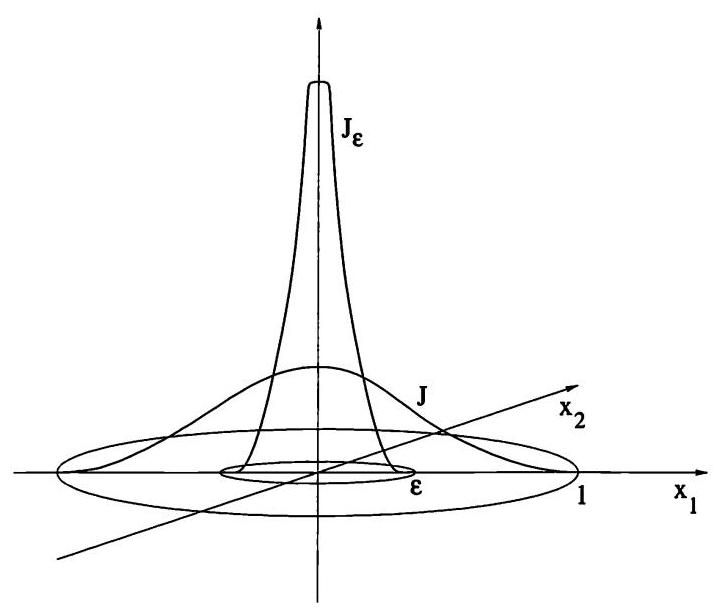
\includegraphics[width=0.6\textwidth]{images/bo_d6ik6nn7aajc739ct1l0_240_398_1533_718_612_0.jpg}
\caption{标准磨光核 $J$ 及其缩放 ${J}_{\varepsilon }$.}
\label{fig:app-A-5-1}
\end{figure}

设 $\Omega  \subseteq  {\mathbb{R}}^{n}$ 为开集， $f \in  {L}_{\text{ loc }}^{1}\left( \Omega \right)$ 为局部可积函数.我们通过卷积定义 $f$ 的磨光:
\[
{f}_{\varepsilon } \doteq  {J}_{\varepsilon } * f
\]

由于 $f$ 定义在 $\Omega$ 上，而 ${J}_{\varepsilon }$ 的支集包含于以原点为中心、半径为 $\varepsilon$ 的球内，该卷积在子集
\[
{\Omega }_{\varepsilon } \doteq  \left\{  {x \in  \Omega ;\overline{B\left( {x,\varepsilon }\right) } \subseteq  \Omega }\right\}  .
\]
中所有点处均有定义.事实上
\[
{f}_{\varepsilon }\left( x\right)  \doteq  {\int }_{B\left( {x,\varepsilon }\right) }{J}_{\varepsilon }\left( {x - y}\right) f\left( y\right) {dy} = {\int }_{B\left( {0,\varepsilon }\right) }{J}_{\varepsilon }\left( z\right) f\left( {x - z}\right) {dz}.
\]

\begin{theorem}[磨光核的性质]\label{thm:app-A-16}
设 $\Omega  \subseteq  {\mathbb{R}}^{n}$ 为开集， $f \in  {L}_{\text{ loc }}^{1}\left( \Omega \right)$ .则:

(i) 对每个 $\varepsilon  > 0$ ，有 ${f}_{\varepsilon } \in  {\mathcal{C}}^{\infty }\left( {\Omega }_{\varepsilon }\right)$ .

(ii) 当 $\varepsilon  \rightarrow  0$ 时，有逐点收敛 ${f}_{\varepsilon }\left( x\right)  \rightarrow  f\left( x\right)$ ，对几乎处处 $x \in  \Omega$ 成立.

(iii) 若 $f$ 连续，则 ${f}_{\varepsilon } \rightarrow  f$ 在 $\Omega$ 的每个紧子集上一致收敛.

(iv) 若 $1 \leq  p < \infty$ 且 $f \in  {L}_{\text{ loc }}^{p}\left( \Omega \right)$ ，则 ${f}_{\varepsilon } \rightarrow  f$ 在 ${L}_{\text{ loc }}^{p}\left( \Omega \right)$ 中成立.
\end{theorem}

\begin{proof}
1. 注意每个 ${\Omega }_{\varepsilon }$ 均为开集.事实上，若闭球 $\overline{B\left( {{x}_{0},\varepsilon }\right) }$ 完全包含于开集 $\Omega$ 中，则当 $\left| {x - {x}_{0}}\right|$ 充分小时，球 $\overline{B\left( {x,\varepsilon }\right) }$ 亦完全包含于 $\Omega$ 中.

设 $\left\{  {{e}_{1},\ldots ,{e}_{n}}\right\}$ 为 ${\mathbb{R}}^{n}$ 的标准标准正交基.固定一点 $x \in  {\Omega }_{\varepsilon }$ 和 $i \in  \{ 1,\ldots ,n\}$ .若 $h$ 足够小，使得 $x + h{e}_{i} \in  {\Omega }_{\varepsilon }$ ，则差商计算为
\begin{align}\tag{A.15}\label{eq:app-A-15}
    &\frac{{f}_{\varepsilon }\left( {x + h{e}_{i}}\right)  - {f}_{\varepsilon }\left( x\right) }{h}\\
    &= \frac{1}{{\varepsilon }^{n}}{\int }_{B\left( {x,\varepsilon }\right) }\frac{1}{h}\left(  {J\left( \frac{x + h{e}_{i} - y}{\varepsilon }\right)  - J\left( \frac{x - y}{\varepsilon }\right) }\right)  f\left( y\right) {dy}.
\end{align}

由于闭球 $\overline{B\left( {x,\varepsilon }\right) }$ 完全包含于 $\Omega$ 中，故有 $f \in \; {L}^{1}\left( {B\left( {x,\varepsilon }\right) }\right)$ .此外，由于 $J \in  {\mathcal{C}}^{\infty }$，我们得到一致收敛
\[
\mathop{\lim }\limits_{{h \rightarrow  0}}\frac{1}{h}\left(  {J\left( \frac{x + h{e}_{i} - y}{\varepsilon }\right)  - J\left( \frac{x - y}{\varepsilon }\right) }\right)   = \frac{1}{\varepsilon }\frac{\partial }{\partial {x}_{i}}J\left( \frac{x - y}{\varepsilon }\right) .
\]

在 \eqref{eq:app-A-15} 式中令 $h \rightarrow  0$ ，可得偏导数的存在性
\[
\frac{\partial }{\partial {x}_{i}}{f}_{\varepsilon }\left( x\right)  = {\int }_{B\left( {x,\varepsilon }\right) }\frac{\partial }{\partial {x}_{i}}{J}_{\varepsilon }\left( {x - y}\right) f\left( y\right) {dy}.
\]

类似论证表明，对任一多重指标 $\alpha$ ，导数 ${D}^{\alpha }{f}_{\varepsilon }$ 存在且
\[
{D}^{\alpha }{f}_{\varepsilon }\left( x\right)  = {\int }_{B\left( {x,\varepsilon }\right) }{D}^{\alpha }{J}_{\varepsilon }\left( {x - y}\right) f\left( y\right) {dy}.
\]

这证明了 (i).

\noindent 2. 由Lebesgue微分定理，对几乎处处的 $x \in  \Omega$ ，有
\begin{equation}\tag{A.16}\label{eq:app-A-16}
\mathop{\lim }\limits_{{r \rightarrow  0}}{f}_{B\left( {x,r}\right) }\left| {f\left( y\right)  - f\left( x\right) }\right| {dy} = 0.
\end{equation}

若 $x$ 是满足 \eqref{eq:app-A-16} 式的点，则
{\begin{align}
    \left| {{f}_{\varepsilon }\left( x\right)  - f\left( x\right) }\right|  &= \left| {{\int }_{B\left( {x,\varepsilon }\right) }{J}_{\varepsilon }\left( {x - y}\right) \left(  {f\left( y\right)  - f\left( x\right) }\right)  {\d y}}\right|\\
    &\leq  \frac{1}{{\varepsilon }^{n}}{\int }_{B\left( {x,\varepsilon }\right) }J\left( \frac{x - y}{\varepsilon }\right) \left| {f\left( y\right)  - f\left( x\right) }\right| {\d y}\\
    &\leq  C{f}_{B\left( {x,\varepsilon }\right) }\left| {f\left( y\right)  - f\left( x\right) }\right| {\d y}.
\end{align}}

当 $\varepsilon  \rightarrow  0$ 时，右端因 \eqref{eq:app-A-16} 而趋于零.这证明了 (ii).

\begin{figure}[htbp]
\centering
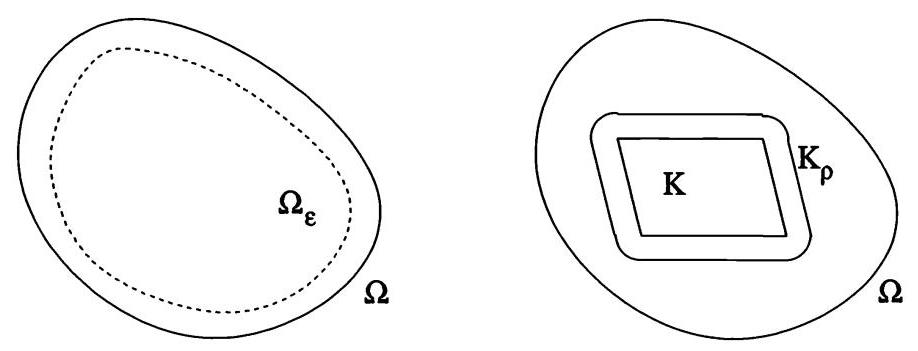
\includegraphics[width=0.8\textwidth]{images/bo_d6ik6nn7aajc739ct1l0_242_301_1360_918_351_0.jpg}
\caption{集合 ${\Omega }_{\varepsilon } \subset  \Omega$ 及紧集 $K \subset   \subset \; {K}_{\rho } \subset   \subset  \Omega$ ，用于磨光子分析.}
\label{fig:app-A-5-2}
\end{figure}

\noindent 3. 假设 $f$ 连续，设 $K \subset  \Omega$ 为一紧子集.则可选取足够小的 $\delta  > 0$ ，使得紧邻域
\begin{equation}\tag{A.17}\label{eq:app-A-17}
{K}_{\rho } \doteq  \left\{  {x \in  {\mathbb{R}}^{n};d\left( {x,K}\right)  \leq  \rho }\right\}
\end{equation}

仍包含于 $\Omega$ 内.由于 $f$ 在紧集 ${K}_{\rho }$ 上一致连续，前述计算表明 ${f}_{\varepsilon }\left( x\right)  \rightarrow  f\left( x\right)$ 对 $x \in  K$ 一致成立.这证明了 (iii).

\noindent 4. 为证明 (iv)，假设 $1 \leq  p < \infty$ 且 $f \in  {L}_{\text{ loc }}^{p}\left( \Omega \right)$ .设 $K \subset  \Omega$ 为一紧子集，并选取 $\rho  > 0$ ，使得 \eqref{eq:app-A-17} 中的紧邻域 ${K}_{\rho }$ 仍包含于 $\Omega$ 内.我们声称:对任意 $0 < \varepsilon  < \rho$ ，有
\begin{equation}\tag{A.18}\label{eq:app-A-18}
{\norm{f}_{\varepsilon }}_{{L}^{p}\left( K\right) } \leq  \| f{\| }_{{L}^{p}\left( {K}_{\rho }\right) }.
\end{equation}

事实上，对 $x \in  K$ ，应用 Hölder 不等式(指数为 $q = \frac{p}{p - 1}$ )可得
{\setjot[-2]\begin{align*}
    \left| {{f}_{\varepsilon }\left( x\right) }\right|  &= \left| {{\int }_{B\left( {x,\varepsilon }\right) }{J}_{\varepsilon }\left( {x - y}\right) f\left( y\right) {\d y}}\right|\\
    &\leq  {\int }_{B\left( {x,\varepsilon }\right) }{\left( {J}_{\varepsilon }\left( x - y\right) \right) }^{\frac{p - 1}{p}}{\left( {J}_{\varepsilon }\left( x - y\right) \right) }^{\frac{1}{p}}\left| {f\left( y\right) }\right| {\d y}\\
    &\leq  {\left( {\int }_{B\left( {x,\varepsilon }\right) }{J}_{\varepsilon }\left( x - y\right) dy\right) }^{\frac{p - 1}{p}}{\left( {\int }_{B\left( {x,\varepsilon }\right) }{J}_{\varepsilon }\left( x - y\right) {\left| f\left( y\right) \right| }^{p}dy\right) }^{\frac{1}{p}}.
\end{align*}}


回顾 ${\int }_{B\left( {x,\varepsilon }\right) }{J}_{\varepsilon }\left( {x - y}\right) {dy} = 1$ ，对 $0 < \varepsilon  < \rho$ ，上述不等式给出
{\setjot[-2]\begin{align*}
    {\int }_{K}{\left| {f}_{\varepsilon }\left( x\right) \right| }^{p}{\d x} &\leq  {\int }_{K}\left( {{\int }_{B\left( {x,\varepsilon }\right) }{J}_{\varepsilon }\left( {x - y}\right) {\left| f\left( y\right) \right| }^{p}{dy}}\right) {\d x}\\
    &\leq  {\int }_{{K}_{\rho }}{\left| f\left( y\right) \right| }^{p}\left( {{\int }_{B\left( {y,\varepsilon }\right) }{J}_{\varepsilon }\left( {x - y}\right) {\d x}}\right) {\d y} = {\int }_{{K}_{\rho }}{\left| f\left( y\right) \right| }^{p}{\d y}.
\end{align*}}

这就证明了 \eqref{eq:app-A-18}.

接下来，对任意 $\delta  > 0$ ，我们选取 $g \in  \mathcal{C}\left( {K}_{\rho }\right)$ 使得
\[
\| f - g{\| }_{{L}^{p}\left( {K}_{\rho }\right) } < \delta
\]

结合\eqref{eq:app-A-18}，可得
{\setjot[-2]\begin{align*}
    {\norm{f_{\varepsilon } - f}}_{{L}^{p}\left( K\right) } &\leq  {\norm{f}_{\varepsilon } - {g}_{\varepsilon }}_{{L}^{p}\left( K\right) } + {\norm{g}_{\varepsilon } - g}_{{L}^{p}\left( K\right) } + \| g - f{\| }_{{L}^{p}\left( K\right) }\\
    &\leq  \| f - g{\| }_{{L}^{p}\left( {K}_{\rho }\right) } + {\norm{g}_{\varepsilon } - g}_{{L}^{p}\left( K\right) } + \| g - f{\| }_{{L}^{p}\left( K\right) }\\
    &\leq  \delta  + {\norm{g}_{\varepsilon } - g}_{{L}^{p}\left( K\right) } + \delta .
\end{align*}}


由于 $g$ 连续，由(ii)可知 $\left| {{g}_{\varepsilon } - g}\right|  \rightarrow  0$ 在紧集 ${K}_{\rho }$ 上一致成立.因此 $\limsup_{{\varepsilon  \rightarrow  0}}{\norm{f_{\varepsilon } - f}}_{{L}^{p}\left( K\right) } \leq  {2\delta }$ .由于 $\delta  > 0$ 是任意的，这便证明了(iv).
\end{proof}

\begin{corollary}\label{cor:app-A-17}
设 $f \in  {L}_{\text{ loc }}^{1}\left( \Omega \right)$ ，并假设
\[
{\int }_{\Omega }{f\phi \d x} = 0,\;\forall\,\phi  \in  {\mathcal{C}}_{\mathrm{c}}^{\infty }\left( \Omega \right) .
\]

则对几乎处处的 $x \in  \Omega$ ，有 $f\left( x\right)  = 0$ .
\end{corollary}

\begin{proof}
事实上，设 $x \in  \Omega$ 为 $f$ 的一个Lebesgue点， ${J}_{\varepsilon }$ 为标准磨光核.取 $\phi \left( y\right)  = {J}_{\varepsilon }\left( {x - y}\right)$，并令 $\varepsilon  \rightarrow  0$，可得
\[
0 = {\int }_{\Omega }{J}_{\varepsilon }\left( {x - y}\right) f\left( y\right) {dy} = {\int }_{B\left( {x,\varepsilon }\right) }J\left( {x - y}\right) f\left( y\right) {dy} \rightarrow  f\left( x\right) .
\]

故对几乎处处的 $x \in  \Omega$ ，有 $f\left( x\right)  = 0$ .
\end{proof}

\subsection{单位分解}
设 $S \subseteq  {\mathbb{R}}^{n}$ ， ${V}_{1},{V}_{2},\ldots$ 为覆盖 $S$ 的一族开集，即
\[
S \subseteq  \mathop{\bigcup }\limits_{{k \geq  1}}{V}_{k}
\]

若一族函数 $\left\{  {{\phi }_{k};k \geq  1}\right\}$ 满足下列条件，则称其为关于集合 ${V}_{k}$ 的光滑单位分解.

(i) 对每个 $k \geq  1,{\phi }_{k} : {\mathbb{R}}^{n} \mapsto  \left(  {0,1}\right)$ ， ${\mathcal{C}}^{\infty }$ 是支撑集包含于开集 ${V}_{k}$ 内的 ${\mathcal{C}}^{\infty }$ 函数.

(ii) 每一点 $x \in  S$ 均存在一个邻域，该邻域仅与有限个函数 ${\phi }_{k}$ 的支撑集相交.此外
\begin{equation}\tag{A.19}\label{eq:app-A-19}
\sum_{k}{\phi }_{k}\left( x\right)  = 1\;\forall\,x \in  S.
\end{equation}

注意，由假设(ii)，在每一点 $x \in  S$ 处，\eqref{eq:app-A-19}式中的求和仅含有限个非零项.

\begin{figure}[htbp]
\centering
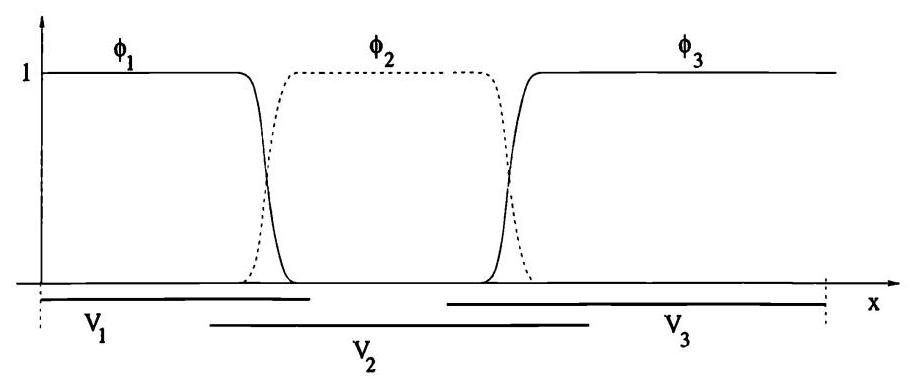
\includegraphics[width=0.8\textwidth]{images/bo_d6ik6nn7aajc739ct1l0_244_301_1743_909_382_0.jpg}
\caption{关于集合 ${V}_{1},{V}_{2},{V}_{3}$ 的单位分解.}
\label{fig:app-A-5-3}
\end{figure}

\begin{theorem}[光滑单位分解的存在性]\label{thm:app-A-18}
设 $S \subseteq \; {\mathbb{R}}^{n}$ ， $\left\{  {{V}_{k};k \geq  1}\right\}$ 为覆盖 $S$ 的一族开集，则存在关于集合 ${V}_{k}$ 的光滑单位分解.
\end{theorem}

\section{不等式}

\subsection{凸集与凸函数}
集合 $\Omega  \subseteq  {\mathbb{R}}^{n}$ 称为凸集，若
\[
x,y \in  \Omega ,\theta  \in  \left(  {0,1}\right)  \implies {\theta x} + \left( {1 - \theta }\right) y \in  \Omega .
\]

换言之，若 $\Omega$ 包含两点 $x,y$ ，则它也包含连接 $x$ 与 $y$ 的整个线段.

设 $\Omega  \subset  {\mathbb{R}}^{n}$ 为一个凸集.若函数 $f : \Omega  \mapsto  \mathbb{R}$ 满足
\begin{equation}\tag{A.20}\label{eq:app-A-20}
f\left( {{\theta x} + \left( {1 - \theta }\right) y}\right)  \leq  {\theta f}\left( x\right)  + \left( {1 - \theta }\right) f\left( y\right)
\end{equation}

对任意 $x,y \in  \Omega$ 和 $\theta  \in  \left(  {0,1}\right)$ 成立，则称其为凸函数.注意，\eqref{eq:app-A-20} 式成立当且仅当 $f$ 的上图(即集合
\[
\{ \left( {x,z}\right)  \in  \Omega  \times  \mathbb{R};z \geq  f\left( x\right) \}
\]
是 ${\mathbb{R}}^{n} \times  \mathbb{R}$ 的一个凸子集.

若二阶可微函数 $f : {\mathbb{R}}^{n} \mapsto  \mathbb{R}$ 的黑塞矩阵(二阶导数矩阵)一致正定，则称其为一致凸函数.这意味着:存在某个常数 $\kappa  > 0$ ，使得
\[
\sum_{{i,j = 1}}^{n}{f}_{{x}_{i}{x}_{j}}\left( x\right) {\xi }_{i}{\xi }_{j} \geq  \kappa \sum_{{i = 1}}^{n}{\xi }_{i}^{2}\;\forall\,x,\xi  \in  {\mathbb{R}}^{n}.
\]

\begin{figure}[htbp]
\centering
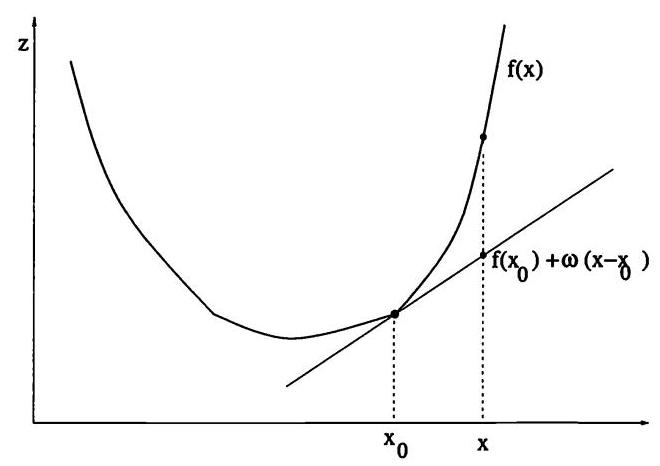
\includegraphics[width=0.6\textwidth]{images/bo_d6ik6nn7aajc739ct1l0_245_426_1636_660_466_0.jpg}
\caption{凸函数 $f$ 及其上图；点 ${x}_{0}$ 处的一个支撑超平面.}
\label{fig:app-A-6-1}
\end{figure}

\begin{theorem}[支撑超平面]\label{thm:app-A-19}
设 $f : {\mathbb{R}}^{n} \mapsto  {\mathbb{R}}^{n}$ 为凸函数，则对每个 ${x}_{0} \in  {\mathbb{R}}^{n}$ ，均存在一个(次梯度)向量 $\omega$ ，使得
\[
f\left( x\right)  \geq  f\left( {x}_{0}\right)  + \left\langle  {\omega ,x - {x}_{0}}\right\rangle  \;\forall\,x \in  {\mathbb{R}}^{n}.
\]

超平面 $\left\{  {\left( {x,z}\right) ;z = \left\langle  {\omega ,x - {x}_{0}}\right\rangle  }\right\}   \subset  {\mathbb{R}}^{n + 1}$ 在点 ${x}_{0}$ 处与 $f$ 的图像相切，且对所有 $x \in  {\mathbb{R}}^{n}$ 均位于该图像下方.因此称其为 $f$ 在 ${x}_{0}$ 处的一个支撑超平面.
\end{theorem}

\begin{theorem}[詹森不等式]\label{thm:app-A-20}
设 $f : \mathbb{R} \mapsto  \mathbb{R}$ 为凸函数， $\Omega  \subset  {\mathbb{R}}^{n}$ 为有界开集.若 $u \in  {L}^{1}\left( \Omega \right)$ 是任一可积函数，则
\begin{equation}\tag{A.21}\label{eq:app-A-21}
f\left( {{\int }_{\Omega }{u\d x}}\right)  \leq  {\oint }_{\Omega }f\left( u\right) {\d x}
\end{equation}
此处 ${f}_{\Omega }{u\d x} \doteq  \frac{1}{\operatorname{meas}\left( \Omega \right) }{\int }_{\Omega }{u\d x}$ 表示 $u$ 在集合 $\Omega$ 上的平均值，而 ${f}_{\Omega }f\left( u\right) {\d x} \doteq  \frac{1}{\operatorname{meas}\left( \Omega \right) }{\int }_{\Omega }f\left( u\right) {\d x}$ 表示 $f\left( u\right)$ 的平均值.注意:我们并不要求集合 $\Omega$ 是凸的.
\end{theorem}

\begin{proof}
令 ${u}_{0} \doteq  {f}_{\Omega }u\left( y\right) {dy}$ .则在点 ${u}_{0}$ 处， $f$ 的图像存在一个支撑超平面，记为 $f\left( u\right)  \geq  f\left( {u}_{0}\right)  + \left\langle  {\omega ,u - {u}_{0}}\right\rangle$ ，其中 $\omega  \in  \mathbb{R}$ 为某常数，且对所有 $u \in  \mathbb{R}$ 成立.故有
\[
f\left( {u\left( x\right) }\right)  \geq  f\left( {{\oint }_{\Omega }u\left( y\right) {dy}}\right) {\d x} + \left\langle  {\omega ,u\left( x\right)  - {\oint }_{\Omega }u\left( y\right) {dy}}\right\rangle  .
\]

对集合 $\Omega$ 上等式两边取平均值，即得 \eqref{eq:app-A-21} 式.
\end{proof}

\subsection{基本不等式.}

\subsubsection{1. Cauchy不等式.}

\begin{equation}\tag{A.22}\label{eq:app-A-22}
{ab} \leq  \frac{{a}^{2} + {b}^{2}}{2}\;\forall\,a,b \in  \mathbb{R}.
\end{equation}

事实上， $0 \leq  {\left( a - b\right) }^{2} = {a}^{2} + {b}^{2} - {2ab}$ .

对任意 $\varepsilon  > 0$ ，在 \eqref{eq:app-A-22} 中将 $a$ 替换为 $\sqrt{2\varepsilon }a$ 、 $b$ 替换为 $b/\sqrt{2\varepsilon }$ ，可得如下稍一般的不等式
\begin{equation}\tag{A.23}\label{eq:app-A-23}
{ab} \leq  \varepsilon {a}^{2} + \frac{{b}^{2}}{4\varepsilon }\;\left( {a,b \in  \mathbb{R},\varepsilon  > 0}\right) .
\end{equation}

\subsubsection*{2. Young不等式.}
\begin{equation}\tag{A.24}\label{eq:app-A-24}
{ab} \leq  \frac{{a}^{p}}{p} + \frac{{b}^{q}}{q}\;\left( {a,b > 0,1 < p < q < \infty ,\frac{1}{p} + \frac{1}{q} = 1}\right) \text{ . }
\end{equation}

事实上，由于映射 $f\left( u\right)  = {e}^{u}$ 是凸的，故有 $\exp \left\{  {\frac{u}{p} + \frac{v}{q}}\right\}   \leq  \frac{{e}^{u}}{p} + \; \frac{{e}^{v}}{q}$ .因此
\[
{ab} = {e}^{\ln a + \ln b} = \exp \left\{  {\frac{1}{p}\ln {a}^{p} + \frac{1}{q}\ln {b}^{q}}\right\}   \leq  \frac{1}{p}{e}^{\ln {a}^{p}} + \frac{1}{q}{e}^{\ln {b}^{q}} = \frac{{a}^{p}}{p} + \frac{{b}^{q}}{q}.
\]

\subsubsection*{3. Hölder不等式.}若 $f \in  {L}^{p}\left( \Omega \right) ,g \in  {L}^{q}\left( \Omega \right)$ ，且 $1 \leq  p,q \leq  \infty$ 、 $\frac{1}{p} + \frac{1}{q} = 1$ ，则
\begin{equation}\tag{A.25}\label{eq:app-A-25}
{\int }_{\Omega }\left| {fg}\right| {\d x} \leq  \| f{\| }_{{L}^{p}\left( \Omega \right) }\| g{\| }_{{L}^{q}\left( \Omega \right) }.
\end{equation}

事实上，在 $\| f{\| }_{{L}^{p}\left( \Omega \right) } = \| g{\| }_{{L}^{q}\left( \Omega \right) } = 1$ 的特殊情形下，杨不等式给出
\[
{\int }_{\Omega }\left| {fg}\right| {\d x} \leq  \frac{1}{p}{\int }_{\Omega }{\left| f\right| }^{p}{\d x} + \frac{1}{q}{\int }_{\Omega }{\left| g\right| }^{q}{\d x} = \frac{1}{p} + \frac{1}{q} = 1 = \| f{\| }_{{L}^{p}}\| g{\| }_{{L}^{q}}.
\]

为涵盖一般情形，我们只需将函数 $f,g$ 分别替换为 $\widetilde{f} = \; f/\| f{\| }_{{L}^{p}}$ 和 $\widetilde{g} = g/\| g{\| }_{{L}^{q}}$ .

通过归纳法，可建立Hölder不等式的如下更一般形式:设 $1 \leq  {p}_{1},\ldots ,{p}_{m} \leq  \infty$ ，且 $\frac{1}{{p}_{1}} + \cdots  + \frac{1}{{p}_{m}} = 1$ ；假设对所有 $k = 1,\ldots ,m$ 均有 ${f}_{k} \in  {L}^{{p}_{k}}\left( \Omega \right)$ ，则
\begin{equation}\tag{A.26}\label{eq:app-A-26}
{\int }_{\Omega }\left| {{f}_{1}{f}_{2}\cdots {f}_{m}}\right| {\d x} \leq  \mathop{\prod }\limits_{{k = 1}}^{m}{\norm{f}_{k}}_{{L}^{{p}_{k}}\left( \Omega \right) }.
\end{equation}

\subsubsection*{4. Minkowski不等式.}对任意 $1 \leq  p \leq  \infty$ 和 $f,g \in  {L}^{p}\left( \Omega \right)$ ，有
\begin{equation}\tag{A.27}\label{eq:app-A-27}
\| f + g{\| }_{{L}^{p}\left( \Omega \right) } \leq  \| f{\| }_{{L}^{p}\left( \Omega \right) } + \| g{\| }_{{L}^{p}\left( \Omega \right) }.
\end{equation}

事实上，当 $p = 1$ 时，结论显然成立；若 $p > 1$ ，将指数分别为 $p$ 和 $q = \frac{p}{p - 1}$ 的Hölder不等式应用于该情形，可得
{\begin{align*}
    {\| f + g\| }_{{L}^{p}\left( \Omega \right) }^{p} &= {\int }_{\Omega }{\left| f + g\right| }^{p}{\d x} = {\int }_{\Omega }{\left| f + g\right| }^{p - 1}\left( {\left| f\right|  + \left| g\right| }\right) {\d x}\\
    &\leq  {\left( {\int }_{\Omega }{\left| f + g\right| }^{\left( {p - 1}\right)  \cdot  \frac{p}{p - 1}}\d x\right) }^{\frac{p - 1}{p}}\left(  {{\left( {\int }_{\Omega }{\left| f\right| }^{p}\d x\right) }^{\frac{1}{p}} + {\left( {\int }_{\Omega }{\left| g\right| }^{p}\d x\right) }^{\frac{1}{p}}}\right) \\
    &= \| f + g{\| }_{{L}^{p}\left( \Omega \right) }^{p - 1}\left( {\| f{\| }_{{L}^{p}\left( \Omega \right) } + \| g{\| }_{{L}^{p}\left( \Omega \right) }}\right) .
\end{align*}}


两边同除以 $\| f + g{\| }_{{L}^{p}\left( \Omega \right) }^{p - 1}$ ，即得\eqref{eq:app-A-27}.

\subsubsection*{5. 插值不等式.}设 $1 \leq  p \leq  r \leq  q \leq  \infty$ ，且满足
\[
\frac{1}{r} = \frac{\theta }{p} + \frac{1 - \theta }{q}\;\text{ 对某个 }\theta  \in  \left(  {0,1}\right)  .
\]

若 $f \in  {L}^{p}\left( \Omega \right)  \cap  {L}^{q}\left( \Omega \right)$ ，则还有 $f \in  {L}^{r}\left( \Omega \right)$ ，且
\begin{equation}\tag{A.28}\label{eq:app-A-28}
\| f{\| }_{{L}^{r}\left( \Omega \right) }\; \leq  \;\| f{\| }_{{L}^{p}\left( \Omega \right) }^{\theta }\| f{\| }_{{L}^{q}\left( \Omega \right) }^{1 - \theta }.
\end{equation}

事实上，注意到 $\frac{\theta r}{p} + \frac{\left( {1 - \theta }\right) r}{q} = 1$ ，由Hölder不等式可得
\begin{align*}
    {\int }_{\Omega }{\left| f\right| }^{r}{\d x} &= {\int }_{\Omega }{\left| f\right| }^{\theta r}{\left| f\right| }^{\left( {1 - \theta }\right) r}{\d x}\\
    &\leq  {\left( {\int }_{\Omega }{\left| f\right| }^{{\theta r} \cdot  \tfrac{p}{{\theta }_{r}}}\d x\right) }^{\tfrac{{\theta }_{r}}{p}}{\left( {\int }_{\Omega }{\left| f\right| }^{\left( {1 - \theta }\right) r \cdot  \tfrac{q}{\left( {1 - \theta }\right) r}}\d x\right) }^{\tfrac{\left( {1 - \theta }\right) r}{q}}
\end{align*}


\subsubsection*{6. 离散型Hölder与Minkowski不等式.}不等式\eqref{eq:app-A-25}与\eqref{eq:app-A-27}更一般地在 $\Omega$ 为任意测度空间时仍成立.特别地，可取 $\Omega  = \{ 1,\ldots ,n\}$ 并赋予计数测度.对任意数组 ${a}_{1},\ldots ,{a}_{n}$ 与 ${b}_{1},\ldots ,{b}_{n}$ ，以及满足 $\frac{1}{p} + \frac{1}{q} = 1$ 的 $1 \leq  p,q < \infty$ ，有离散型Hölder不等式
\begin{equation}\tag{A.29}\label{eq:app-A-29}
\sum_{{k = 1}}^{n}\left| {{a}_{k}{b}_{k}}\right|  \leq  {\left( \sum_{{k = 1}}^{n}{\left| {a}_{k}\right| }^{p}\right) }^{\frac{1}{p}}{\left( \sum_{{k = 1}}^{n}{\left| {b}_{k}\right| }^{q}\right) }^{\frac{1}{q}}
\end{equation}
及离散型Minkowski不等式
\begin{equation}\tag{A.30}\label{eq:app-A-30}
{\left( \sum_{{k = 1}}^{n}{\left| {a}_{k} + {b}_{k}\right| }^{p}\right) }^{\frac{1}{p}} \leq  {\left( \sum_{{k = 1}}^{n}{\left| {a}_{k}\right| }^{p}\right) }^{\frac{1}{p}} + {\left( \sum_{{k = 1}}^{n}{\left| {b}_{k}\right| }^{p}\right) }^{\frac{1}{p}}
\end{equation}

给定两个向量 $x = \left( {{x}_{1},\ldots ,{x}_{n}}\right)$ 和 $y = \left( {{y}_{1},\ldots ,{y}_{n}}\right)$ ，在 $p = q = 2$ 下应用离散 Hölder 不等式\eqref{eq:app-A-29}，可得定义在 ${\mathbb{R}}^{n}$ 上的内积的 Cauchy-Schwarz 不等式:
\begin{equation}\tag{A.31}\label{eq:app-A-31}
\left| {\langle x,y\rangle }\right|  \leq  \left| x\right| \left| y\right| .
\end{equation}

事实上，
\[
\left| {\langle x,y\rangle }\right|  = \left| {\sum_{{k = 1}}^{n}{x}_{k}{y}_{k}}\right|  \leq  \sum_{{k = 1}}^{n}\left| {{x}_{k}{y}_{k}}\right|  \leq  {\left( \sum_{{k = 1}}^{n}{\left| {x}_{k}\right| }^{2}\right) }^{\frac{1}{2}}{\left( \sum_{{k = 1}}^{n}{\left| {y}_{k}\right| }^{2}\right) }^{\frac{1}{2}} = \left| x\right| \left| y\right| .
\]

\subsection{一个微分不等式.}

\begin{theorem}[Gronwall 不等式]\label{thm:app-A-21}
设 $t \mapsto  z\left( t\right)$ 是定义在 $t \in  \left(  {0,T}\right)$ 上的非负绝对连续函数.假设其时间导数 ${z}^{\prime } = \frac{\d}{\d t}z$ 满足
\[
{z}^{\prime }\left( t\right)  \leq  \phi \left( t\right) z\left( t\right)  + \psi \left( t\right) \;\text{ for a.e. }t \in  \left(  {0,T}\right)  ,
\]

其中 $\phi ,\psi  \in  {L}^{1}\left( \left(  {0,T}\right)  \right)$ 为非负函数.则有\eqref{eq:app-A-32}
\begin{equation}\tag{A.32}\label{eq:app-A-32}
z\left( t\right) \; \leq  \;{e}^{{\int }_{0}^{t}\phi \left( s\right) \;{ds}}z\left( 0\right) \; + \;{\int }_{0}^{t}{e}^{{\int }_{s}^{t}\phi \left( \sigma \right) \;{d\sigma }}\psi \left( s\right){\d s}\;\forall\,\;t \in  \left(  {0,T}\right)  .
\end{equation}
\end{theorem}

\begin{proof}
注意，\eqref{eq:app-A-32} 右端恰好是初值问题
\[
{Z}^{\prime }\left( t\right)  = \phi \left( t\right) Z\left( t\right)  + \psi \left( t\right) ,\;Z\left( 0\right)  = z\left( 0\right) .
\]

为证明 \eqref{eq:app-A-32}，我们写出
\[
\frac{\d}{\d s}\left( {{e}^{-{\int }_{0}^{s}\phi \left( \sigma \right) \;{d\sigma }}z\left( s\right) }\right) \; = \;{e}^{-{\int }_{0}^{s}\phi \left( \sigma \right) \;{d\sigma }}\left( {{z}^{\prime }\left( s\right)  - \phi \left( s\right) z\left( s\right) }\right) \; \leq  \;{e}^{-{\int }_{0}^{s}\phi \left( \sigma \right) \;{d\sigma }}\psi \left( s\right) .
\]

在区间 $\left(  {0,t}\right)$ 上积分，得
\[
{e}^{-{\int }_{0}^{t}\phi \left( \sigma \right) {d\sigma }}z\left( t\right)  - z\left( 0\right)  \leq  {\int }_{0}^{t}{e}^{-{\int }_{0}^{s}\phi \left( \sigma \right) {d\sigma }}\psi \left( s\right) {\d s}.
\]

两边同乘 ${e}^{{\int }_{0}^{t}\phi \left( \sigma \right) {\d \sigma }}$ ，即得 \eqref{eq:app-A-32}.
\end{proof}

\section{习题}

\begin{rbhw}[index=1]
设 $\left\{  {{A}_{i};i \in  \mathcal{I}}\right\}$ 是紧致度量空间 $K$ 的一个开覆盖.证明存在 $\rho  > 0$ ，使得对任意 $x \in  K$ ，球 $B\left( {x,\rho }\right)$ 完全包含于某个集合 ${A}_{i}$ 中.
\end{rbhw}

\begin{rbhw}
    设 ${\left( {x}_{n}\right) }_{n \geq  1}$ 是度量空间 $E$ 中的一列点.证明下列命题.
    \begin{enumerate}[(i)]
        \item 该序列收敛于某点 $\bar{x}$ 当且仅当从任意子列 ${\left( {x}_{{n}_{j}}\right) }_{j \geq  1}$ 中均可再选出一个收敛于 $\bar{x}$ 的子列.
        \item 若对所有 $m \neq  n$ 均有 $d\left( {{x}_{m},{x}_{n}}\right)  \geq  \delta  > 0$ ，则不存在收敛子列.
        \item 设 $E$ 是完备的，且假设对任意 $\varepsilon  > 0$ ，从任一序列中均可再选出一个子列 ${\left( {x}_{{n}_{j}}\right) }_{j \geq  1}$，使得
\[
\limsup_{{j,k \rightarrow  \infty }}d\left( {{x}_{{n}_{j}},{x}_{{n}_{k}}}\right)  < \varepsilon
\]
则该序列存在收敛子列.
    \end{enumerate}
\end{rbhw}


\begin{rbhw}
考虑函数
\[
f\left( x\right)  = \left\{  \begin{matrix} \frac{1}{x{\left( \ln x\right) }^{2}} & \text{ if }0 < x < \frac{1}{2}, \\  0 & \text{ otherwise. } \end{matrix}\right.
\]

设 ${f}_{\varepsilon } \doteq  {J}_{\varepsilon } * f$ 为其对应的磨光函数，并令
\[
F\left( x\right)  \doteq  \mathop{\sup }\limits_{{0 < \varepsilon  < 1}}{f}_{\varepsilon }\left( x\right)
\]

证明 $f \in  {L}^{1}\left( \mathbb{R}\right)$ 成立，但 $F \notin  {L}^{1}\left( \mathbb{R}\right)$ 不成立.因此，尽管 ${f}_{\varepsilon } \rightarrow  f$ 逐点成立，却无法利用Lebesgue控制收敛定理证明 ${\norm{f}_{\varepsilon } - f}_{{L}^{1}\left( \mathbb{R}\right) } \rightarrow  0$ .
\end{rbhw}

\begin{rbhw}
设 ${f}_{n} : \mathbb{R} \mapsto  \mathbb{R},n \geq  1$ 为一列绝对连续函数，满足
\begin{enumerate}[(i)]
    \item 在点 $x = 0$ 处，序列 ${f}_{n}\left( 0\right)$ 有界；
    \item 存在函数 $g \in  {L}^{1}\left( \mathbb{R}\right)$ ，使得其导数 ${f}_{n}^{\prime }$ 对每个 $n \geq  1$ 及几乎处处 $x \in  \mathbb{R}.$ 满足 $\left| {{f}_{n}^{\prime }\left( x\right) }\right|  \leq  g\left( x\right)$ .
\end{enumerate}
证明:存在子列 ${\left( {f}_{{n}_{j}}\right) }_{j \geq  1}$ ，在全体实轴上一致收敛.
\end{rbhw}

\begin{rbhw}
考虑一列函数 ${f}_{n} \in  {L}^{1}\left( \mathbb{R}\right)$ ，满足对每个 $n \geq  1$ 均有 ${\norm{f}_{n}}_{{L}^{1}} \leq  C$ .定义
\[
f\left( x\right)  \doteq  \left\{  \begin{matrix} \mathop{\lim }\limits_{{n \rightarrow  \infty }}{f}_{n}\left( x\right) & \text{ if the limit exists, } \\  0 & \text{ otherwise. } \end{matrix}\right.
\]

证明: $f$ 是Lebesgue可测的，且 $\| f{\| }_{{L}^{1}} \leq  C$ .
\end{rbhw}

\begin{rbhw}
设 $f : \mathbb{R} \rightarrow  \mathbb{R}$ 为绝对连续函数.证明: $f$ 将Lebesgue测度为零的集合映为Lebesgue测度为零的集合.
\end{rbhw}

\begin{rbhw}
(i) 若 ${\left( {f}_{n}\right) }_{n \geq  1}$ 是 ${L}^{1}\left( \left(  {0,1}\right)  \right)$ 中的一列函数，且满足 ${\norm{f}_{n}}_{{L}^{1}} \rightarrow  0$ ，则证明存在一子列在几乎处处 $x \in  \left(  {0,1}\right)$ 点态收敛.


(ii) 构造一列可测函数 ${f}_{n} : \left(  {0,1}\right)   \mapsto  \left(  {0,1}\right)$ ，使得 ${\norm{f}_{n}}_{{L}^{1}} \rightarrow  0$ 成立，但对每个 $x \in  \left(  {0,1}\right)$，序列 ${f}_{n}\left( x\right)$ 均无极限.
\end{rbhw}

\begin{rbhw}
对任意(非空)开集 $\Omega  \subseteq  {\mathbb{R}}^{n}$ 及 $1 \leq  p \leq  \infty$ ，证明空间 ${L}^{p}\left( \Omega \right)$ 是无限维的.构造一列函数 ${\left( {f}_{j}\right) }_{j \geq  1}$ ，使得
\[
{\norm{f}_{j}}_{{L}^{p}} = 1,\;{\norm{f}_{i} - {f}_{j}}_{{L}^{p}} \geq  1\;\forall\,i,j \geq  1,i \neq  j.
\]
\end{rbhw}

\begin{rbhw}
考虑集合 ${\mathbb{R}}^{2}$ ，其上赋予偏序关系
\[
x \preccurlyeq  y \iff {x}_{1} \leq  {y}_{1}\text{ and }{x}_{2} \leq  {y}_{2}.
\]

设 $f : \mathbb{R} \mapsto  \mathbb{R}$ 为连续、非减函数.证明集合
\[
S \doteq  \operatorname{Graph}\left( f\right)  = \{ \left( {t,f\left( t\right) }\right) ;t \in  \mathbb{R}\}
\]

是 ${\mathbb{R}}^{2}$ 的一个极大全序子集.是否每个极大全序子集均可由此方式得到？
\end{rbhw}

\begin{rbhw}
给出广义Hölder不等式\eqref{eq:app-A-26}的证明.
\end{rbhw}

\chapter{符号说明汇总}

$\mathbb{R}$ ，实数域.

$\mathbb{C}$ ，复数域.

$\mathbb{K}$ ，一个数域，为 $\mathbb{R}$ 或 $\mathbb{C}$ .

Re $z$ 和 $\operatorname{Im}z$ ，复数 $z$ 的实部与虚部.

$\bar{z} = a - {ib}$ ，数 $z = a + {ib} \in  \mathbb{C}$ 的复共轭.

$\left(  {a,b}\right)$ ，闭区间； $( a,b\left(  \text{ , an open interval; }\right)  a,b( ,) a,b)$ 为半开区间.

${\mathbb{R}}^{n}$ ， $n$ 维欧几里得空间.

$\langle  \cdot  , \cdot  \rangle$ ，欧几里得空间 ${\mathbb{R}}^{n}$ 上的标量积.

$\left| v\right|  \doteq  \sqrt{\langle v,v\rangle }$ ，向量 $v \in  {\mathbb{R}}^{n}$ 的欧几里得长度.

$A \setminus  B \doteq  \{ x \in  A,x \notin  B\}$ ，集合的差集.

$\bar{A}$ ，集合 $A$ 的闭包.

$\partial A$ ，集合 $A$ 的边界.

${\Omega }^{\prime } \subset   \subset  \Omega$ ， ${\Omega }^{\prime }$ 的闭包是 $\Omega$ 的紧子集.

${\chi }_{A}$ ，集合 $A.{\chi }_{A}\left( x\right)  = \left\{  \begin{array}{ll} 1 & \text{ if }x \in  A, \\  0 & \text{ if }x \notin  A. \end{array}\right.$ 的示性函数.

$f : A \mapsto  B$ ，从集合 $A$ 到集合 $B$ 的映射.

$a \mapsto  b = f\left( a\right)$ ，函数 $f$ 将元素 $a \in  A$ 映为元素 $b \in  B$ .

$\doteq$ ，定义相等.

$\Leftrightarrow$ ，当且仅当.

$\mathcal{C}\left( E\right)  = \mathcal{C}\left( {E,\mathbb{R}}\right)$ ，度量空间 $E$ 上所有连续实值函数构成的向量空间.

$\mathcal{C}\left( {E,\mathbb{C}}\right)$ ，度量空间 $E$ 上所有连续复值函数构成的向量空间.

$\mathcal{B}C\left( E\right)$ ， $f : E \mapsto \; \mathbb{R}$ 上所有有界连续实值函数构成的空间，其范数为 $\| f\|  = \mathop{\sup }\limits_{{x \in  E}}\left| {f\left( x\right) }\right|$ .

${\ell }^{1},{\ell }^{p},{\ell }^{\infty }$ ，实数(或复数)序列空间.

${L}^{1}\left( \Omega \right) ,{L}^{p}\left( \Omega \right) ,{L}^{\infty }\left( \Omega \right)$ ，Lebesgue空间.

${W}^{k,p}\left( \Omega \right)$ ，Soblev空间，即定义在某个开集 $\Omega  \subseteq  {\mathbb{R}}^{n}$ 上的函数空间，其阶数不超过 $k$ 的弱偏导数属于 ${L}^{p}\left( \Omega \right)$ .
\[
{H}^{k}\left( \Omega \right)  = {W}^{k,2}\left( \Omega \right) \text{ , Hilbert-Soblev 空间. }
\]

${\mathcal{C}}^{k,\gamma }\left( \Omega \right)$ ，Hölder空间，即函数 $u : \Omega  \mapsto  \mathbb{R}$ 构成的空间，其阶数不超过 $k$ 的导数具有指数为 $\gamma  \in  (0,1)$ 的Hölder连续性.

$\|  \cdot  \|  = \|  \cdot  {\| }_{X}$ ，向量空间 $X$ 上的范数.

$\left( {\cdot , \cdot  }\right)  = {\left( \cdot , \cdot  \right) }_{H}$ ，Hilbert空间 $H$ 上的内积.

${X}^{ * }$ ， $X$ 的对偶空间，即所有连续线性泛函 ${x}^{ * } : X \mapsto  \mathbb{K}$ 构成的空间.

$\left\langle  {{x}^{ * },x}\right\rangle   = {x}^{ * }\left( x\right)$ ， ${x}^{ * } \in  {X}^{ * }$ 与 $x \in  X$ 之间的对偶积.

${x}_{n} \rightarrow  x$ ，按范数强收敛；即 $\norm{{x}_{n} - x} \rightarrow  0$ .

${x}_{n} \rightharpoonup  x$ ，弱收敛.

${\varphi }_{n}\overset{ * }{ \rightharpoonup  }\varphi$ ，弱*收敛.

$f * g$ ，两个函数 $f,g : {\mathbb{R}}^{n} \mapsto  \mathbb{R}$ 的卷积.

$\nabla u = \left( {{u}_{{x}_{1}},{u}_{{x}_{2}},\ldots ,{u}_{{x}_{n}}}\right)$ ，函数 $u : {\mathbb{R}}^{n} \mapsto  \mathbb{R}$ 的梯度.

${D}^{\alpha } = {\left( \frac{\partial }{\partial {x}_{1}}\right) }^{{\alpha }_{1}}{\left( \frac{\partial }{\partial {x}_{2}}\right) }^{{\alpha }_{2}}\cdots {\left( \frac{\partial }{\partial {x}_{n}}\right) }^{{\alpha }_{n}} = {\partial }_{{x}_{1}}^{{\alpha }_{1}}{\partial }_{{x}_{2}}^{{\alpha }_{2}}\cdots {\partial }_{{x}_{n}}^{{\alpha }_{n}}$ ，一个阶数为 $\left| \alpha \right|  \doteq  {\alpha }_{1} + {\alpha }_{2} + \cdots  + {\alpha }_{n}$ 的偏微分算子.

meas $\left( \Omega \right)$ ，集合 $\Omega  \subset  {\mathbb{R}}^{n}$ 的Lebesgue测度.

${f}_{\Omega }{f\d x} = \frac{1}{\operatorname{meas}\left( \Omega \right) }{\int }_{\Omega }{f\d x}$ ， $f$ 在集合 $\Omega$ 上的平均值.


\end{document}